\documentclass[twoside]{book}

% Packages required by doxygen
\usepackage{fixltx2e}
\usepackage{calc}
\usepackage{doxygen}
\usepackage[export]{adjustbox} % also loads graphicx
\usepackage{graphicx}
\usepackage[utf8]{inputenc}
\usepackage{makeidx}
\usepackage{multicol}
\usepackage{multirow}
\PassOptionsToPackage{warn}{textcomp}
\usepackage{textcomp}
\usepackage[nointegrals]{wasysym}
\usepackage[table]{xcolor}

% Font selection
\usepackage[T1]{fontenc}
\usepackage[scaled=.90]{helvet}
\usepackage{courier}
\usepackage{amssymb}
\usepackage{sectsty}
\renewcommand{\familydefault}{\sfdefault}
\allsectionsfont{%
  \fontseries{bc}\selectfont%
  \color{darkgray}%
}
\renewcommand{\DoxyLabelFont}{%
  \fontseries{bc}\selectfont%
  \color{darkgray}%
}
\newcommand{\+}{\discretionary{\mbox{\scriptsize$\hookleftarrow$}}{}{}}

% Page & text layout
\usepackage{geometry}
\geometry{%
  a4paper,%
  top=2.5cm,%
  bottom=2.5cm,%
  left=2.5cm,%
  right=2.5cm%
}
\tolerance=750
\hfuzz=15pt
\hbadness=750
\setlength{\emergencystretch}{15pt}
\setlength{\parindent}{0cm}
\setlength{\parskip}{3ex plus 2ex minus 2ex}
\makeatletter
\renewcommand{\paragraph}{%
  \@startsection{paragraph}{4}{0ex}{-1.0ex}{1.0ex}{%
    \normalfont\normalsize\bfseries\SS@parafont%
  }%
}
\renewcommand{\subparagraph}{%
  \@startsection{subparagraph}{5}{0ex}{-1.0ex}{1.0ex}{%
    \normalfont\normalsize\bfseries\SS@subparafont%
  }%
}
\makeatother

% Headers & footers
\usepackage{fancyhdr}
\pagestyle{fancyplain}
\fancyhead[LE]{\fancyplain{}{\bfseries\thepage}}
\fancyhead[CE]{\fancyplain{}{}}
\fancyhead[RE]{\fancyplain{}{\bfseries\leftmark}}
\fancyhead[LO]{\fancyplain{}{\bfseries\rightmark}}
\fancyhead[CO]{\fancyplain{}{}}
\fancyhead[RO]{\fancyplain{}{\bfseries\thepage}}
\fancyfoot[LE]{\fancyplain{}{}}
\fancyfoot[CE]{\fancyplain{}{}}
\fancyfoot[RE]{\fancyplain{}{\bfseries\scriptsize Generated by Doxygen }}
\fancyfoot[LO]{\fancyplain{}{\bfseries\scriptsize Generated by Doxygen }}
\fancyfoot[CO]{\fancyplain{}{}}
\fancyfoot[RO]{\fancyplain{}{}}
\renewcommand{\footrulewidth}{0.4pt}
\renewcommand{\chaptermark}[1]{%
  \markboth{#1}{}%
}
\renewcommand{\sectionmark}[1]{%
  \markright{\thesection\ #1}%
}

% Indices & bibliography
\usepackage{natbib}
\usepackage[titles]{tocloft}
\setcounter{tocdepth}{3}
\setcounter{secnumdepth}{5}
\makeindex

% Hyperlinks (required, but should be loaded last)
\usepackage{ifpdf}
\ifpdf
  \usepackage[pdftex,pagebackref=true]{hyperref}
\else
  \usepackage[ps2pdf,pagebackref=true]{hyperref}
\fi
\hypersetup{%
  colorlinks=true,%
  linkcolor=blue,%
  citecolor=blue,%
  unicode%
}

% Custom commands
\newcommand{\clearemptydoublepage}{%
  \newpage{\pagestyle{empty}\cleardoublepage}%
}

\usepackage{caption}
\captionsetup{labelsep=space,justification=centering,font={bf},singlelinecheck=off,skip=4pt,position=top}

%===== C O N T E N T S =====

\begin{document}

% Titlepage & ToC
\hypersetup{pageanchor=false,
             bookmarksnumbered=true,
             pdfencoding=unicode
            }
\pagenumbering{roman}
\begin{titlepage}
\vspace*{7cm}
\begin{center}%
{\Large My Project }\\
\vspace*{1cm}
{\large Generated by Doxygen 1.8.11}\\
\end{center}
\end{titlepage}
\clearemptydoublepage
\tableofcontents
\clearemptydoublepage
\pagenumbering{arabic}
\hypersetup{pageanchor=true}

%--- Begin generated contents ---
\chapter{Projet int�grateur de deuxi�me ann�e -\/-\/ I\+N\+F2990}
\label{index}\hypertarget{index}{}\input{index}
\chapter{Module Index}
\section{Modules}
Here is a list of all modules\+:\begin{DoxyCompactList}
\item \contentsline{section}{I\+N\+F2990}{\pageref{group__inf2990}}{}
\end{DoxyCompactList}

\chapter{Namespace Index}
\section{Namespace List}
Here is a list of all documented namespaces with brief descriptions\+:\begin{DoxyCompactList}
\item\contentsline{section}{\hyperlink{namespace_interface_graphique}{Interface\+Graphique} }{\pageref{namespace_interface_graphique}}{}
\item\contentsline{section}{\hyperlink{namespace_interface_graphique_1_1_properties}{Interface\+Graphique.\+Properties} }{\pageref{namespace_interface_graphique_1_1_properties}}{}
\item\contentsline{section}{\hyperlink{namespacemodele}{modele} \\*D�clarations avanc�es pour contenir un pointeur vers un mod�le3D et son storage }{\pageref{namespacemodele}}{}
\end{DoxyCompactList}

\chapter{Hierarchical Index}
\section{Class Hierarchy}
This inheritance list is sorted roughly, but not completely, alphabetically\+:\begin{DoxyCompactList}
\item \contentsline{section}{Etat\+Abstrait}{\pageref{class_etat_abstrait}}{}
\begin{DoxyCompactList}
\item \contentsline{section}{Etat\+Creation\+Ligne}{\pageref{class_etat_creation_ligne}}{}
\item \contentsline{section}{Etat\+Creation\+Mur}{\pageref{class_etat_creation_mur}}{}
\item \contentsline{section}{Etat\+Creation\+Poteau}{\pageref{class_etat_creation_poteau}}{}
\item \contentsline{section}{Etat\+Deplacement}{\pageref{class_etat_deplacement}}{}
\item \contentsline{section}{Etat\+Duplication}{\pageref{class_etat_duplication}}{}
\item \contentsline{section}{Etat\+Loupe}{\pageref{class_etat_loupe}}{}
\item \contentsline{section}{Etat\+Mise\+A\+Echelle}{\pageref{class_etat_mise_a_echelle}}{}
\item \contentsline{section}{Etat\+Rotation}{\pageref{class_etat_rotation}}{}
\item \contentsline{section}{Etat\+Selection}{\pageref{class_etat_selection}}{}
\end{DoxyCompactList}
\item \contentsline{section}{Facade\+Modele}{\pageref{class_facade_modele}}{}
\item Form\begin{DoxyCompactList}
\item \contentsline{section}{Interface\+Graphique.\+Explorateur\+Ouverture}{\pageref{class_interface_graphique_1_1_explorateur_ouverture}}{}
\item \contentsline{section}{Interface\+Graphique.\+Explorateur\+Sauvegarde}{\pageref{class_interface_graphique_1_1_explorateur_sauvegarde}}{}
\item \contentsline{section}{Interface\+Graphique.\+Nouveau\+Fichier}{\pageref{class_interface_graphique_1_1_nouveau_fichier}}{}
\item \contentsline{section}{Interface\+Graphique.\+Pop\+Out\+Interface}{\pageref{class_interface_graphique_1_1_pop_out_interface}}{}
\item \contentsline{section}{Interface\+Graphique.\+Window}{\pageref{class_interface_graphique_1_1_window}}{}
\end{DoxyCompactList}
\item I\+Message\+Filter\begin{DoxyCompactList}
\item \contentsline{section}{Interface\+Graphique.\+Window}{\pageref{class_interface_graphique_1_1_window}}{}
\end{DoxyCompactList}
\item \contentsline{section}{Interface\+Graphique.\+Menu\+Edition\+Nouveau}{\pageref{class_interface_graphique_1_1_menu_edition_nouveau}}{}
\item \contentsline{section}{Interface\+Graphique.\+Fonctions\+Natives.\+Message}{\pageref{struct_interface_graphique_1_1_fonctions_natives_1_1_message}}{}
\item \contentsline{section}{Mode\+Abstrait}{\pageref{class_mode_abstrait}}{}
\begin{DoxyCompactList}
\item \contentsline{section}{Mode\+Configure}{\pageref{class_mode_configure}}{}
\item \contentsline{section}{Mode\+Edition}{\pageref{class_mode_edition}}{}
\item \contentsline{section}{Mode\+Menu\+Principal}{\pageref{class_mode_menu_principal}}{}
\item \contentsline{section}{Mode\+Simulation}{\pageref{class_mode_simulation}}{}
\item \contentsline{section}{Mode\+Test}{\pageref{class_mode_test}}{}
\end{DoxyCompactList}
\item \contentsline{section}{Noeud\+Abstrait}{\pageref{class_noeud_abstrait}}{}
\begin{DoxyCompactList}
\item \contentsline{section}{Noeud\+Composite}{\pageref{class_noeud_composite}}{}
\begin{DoxyCompactList}
\item \contentsline{section}{Arbre\+Rendu}{\pageref{class_arbre_rendu}}{}
\begin{DoxyCompactList}
\item \contentsline{section}{Arbre\+Rendu\+I\+N\+F2990}{\pageref{class_arbre_rendu_i_n_f2990}}{}
\end{DoxyCompactList}
\item \contentsline{section}{Noeud\+Duplication}{\pageref{class_noeud_duplication}}{}
\item \contentsline{section}{Noeud\+Ligne}{\pageref{class_noeud_ligne}}{}
\item \contentsline{section}{Noeud\+Robot}{\pageref{class_noeud_robot}}{}
\item \contentsline{section}{Noeud\+Table}{\pageref{class_noeud_table}}{}
\end{DoxyCompactList}
\item \contentsline{section}{Noeud\+Depart}{\pageref{class_noeud_depart}}{}
\item \contentsline{section}{Noeud\+Jonction}{\pageref{class_noeud_jonction}}{}
\item \contentsline{section}{Noeud\+Mur}{\pageref{class_noeud_mur}}{}
\item \contentsline{section}{Noeud\+Poteau}{\pageref{class_noeud_poteau}}{}
\item \contentsline{section}{Noeud\+Segment}{\pageref{class_noeud_segment}}{}
\end{DoxyCompactList}
\item Singleton\begin{DoxyCompactList}
\item \contentsline{section}{Banc\+Tests}{\pageref{class_banc_tests}}{}
\item \contentsline{section}{Config\+Scene}{\pageref{class_config_scene}}{}
\end{DoxyCompactList}
\item Test\+Fixture\begin{DoxyCompactList}
\item \contentsline{section}{Config\+Scene\+Test}{\pageref{class_config_scene_test}}{}
\item \contentsline{section}{Noeud\+Abstrait\+Test}{\pageref{class_noeud_abstrait_test}}{}
\end{DoxyCompactList}
\item \contentsline{section}{Usine\+Abstraite}{\pageref{class_usine_abstraite}}{}
\begin{DoxyCompactList}
\item \contentsline{section}{Usine\+Noeud$<$ Noeud $>$}{\pageref{class_usine_noeud}}{}
\end{DoxyCompactList}
\item \contentsline{section}{Visiteur\+Abstrait}{\pageref{class_visiteur_abstrait}}{}
\begin{DoxyCompactList}
\item \contentsline{section}{Visiteur\+Creation\+Ligne}{\pageref{class_visiteur_creation_ligne}}{}
\item \contentsline{section}{Visiteur\+Creation\+Mur}{\pageref{class_visiteur_creation_mur}}{}
\item \contentsline{section}{Visiteur\+Creation\+Poteau}{\pageref{class_visiteur_creation_poteau}}{}
\item \contentsline{section}{Visiteur\+Deplacement}{\pageref{class_visiteur_deplacement}}{}
\item \contentsline{section}{Visiteur\+Duplication}{\pageref{class_visiteur_duplication}}{}
\item \contentsline{section}{Visiteur\+Mise\+A\+Echelle}{\pageref{class_visiteur_mise_a_echelle}}{}
\item \contentsline{section}{Visiteur\+Mise\+A\+Jour\+Quad}{\pageref{class_visiteur_mise_a_jour_quad}}{}
\item \contentsline{section}{Visiteur\+Rotation}{\pageref{class_visiteur_rotation}}{}
\item \contentsline{section}{Visiteur\+Sauvegarde}{\pageref{class_visiteur_sauvegarde}}{}
\item \contentsline{section}{Visiteur\+Selection}{\pageref{class_visiteur_selection}}{}
\item \contentsline{section}{Visiteur\+Suppression}{\pageref{class_visiteur_suppression}}{}
\item \contentsline{section}{Visiteur\+Verification\+Quad}{\pageref{class_visiteur_verification_quad}}{}
\end{DoxyCompactList}
\end{DoxyCompactList}

\chapter{Class Index}
\section{Class List}
Here are the classes, structs, unions and interfaces with brief descriptions\+:\begin{DoxyCompactList}
\item\contentsline{section}{\hyperlink{class_arbre_rendu}{Arbre\+Rendu} \\*Classe d\textquotesingle{}arbre de rendu qui contient la racine de l\textquotesingle{}arbre de rendu avec les usines qui permettent d\textquotesingle{}ajouter des noeuds � cet arbre }{\pageref{class_arbre_rendu}}{}
\item\contentsline{section}{\hyperlink{class_arbre_rendu_i_n_f2990}{Arbre\+Rendu\+I\+N\+F2990} \\*Classe qui repr�sente l\textquotesingle{}arbre de rendu sp�cifique au projet de I\+N\+F2990 }{\pageref{class_arbre_rendu_i_n_f2990}}{}
\item\contentsline{section}{\hyperlink{class_banc_tests}{Banc\+Tests} \\*Banc de tests qui permet d\textquotesingle{}ex�cuter tous les tests unitaires. C\textquotesingle{}est une classe singleton }{\pageref{class_banc_tests}}{}
\item\contentsline{section}{\hyperlink{class_config_scene}{Config\+Scene} \\*Les variables de configuration de la classe C\+Scene. C\textquotesingle{}est une classe singleton }{\pageref{class_config_scene}}{}
\item\contentsline{section}{\hyperlink{class_config_scene_test}{Config\+Scene\+Test} \\*Classe de test cppunit pour tester le bon fonctionnement des m�thodes de la classe \hyperlink{class_config_scene}{Config\+Scene} }{\pageref{class_config_scene_test}}{}
\item\contentsline{section}{\hyperlink{class_etat_abstrait}{Etat\+Abstrait} \\*Classe de base pour chaque �tat }{\pageref{class_etat_abstrait}}{}
\item\contentsline{section}{\hyperlink{class_etat_creation_ligne}{Etat\+Creation\+Ligne} \\*�tat repr�sentant la creation d\textquotesingle{}une ligne }{\pageref{class_etat_creation_ligne}}{}
\item\contentsline{section}{\hyperlink{class_etat_creation_mur}{Etat\+Creation\+Mur} \\*�tat repr�sentant la creation d\textquotesingle{}un mur }{\pageref{class_etat_creation_mur}}{}
\item\contentsline{section}{\hyperlink{class_etat_creation_poteau}{Etat\+Creation\+Poteau} \\*�tat repr�sentant la creation d\textquotesingle{}un poteau }{\pageref{class_etat_creation_poteau}}{}
\item\contentsline{section}{\hyperlink{class_etat_deplacement}{Etat\+Deplacement} \\*�tat repr�sentant le d�placement d\textquotesingle{}un objet }{\pageref{class_etat_deplacement}}{}
\item\contentsline{section}{\hyperlink{class_etat_duplication}{Etat\+Duplication} \\*�tat repr�sentant la duplication d\textquotesingle{}un objet }{\pageref{class_etat_duplication}}{}
\item\contentsline{section}{\hyperlink{class_etat_loupe}{Etat\+Loupe} \\*�tat repr�sentant le zoom sur une partie de l\textquotesingle{}�cran }{\pageref{class_etat_loupe}}{}
\item\contentsline{section}{\hyperlink{class_etat_mise_a_echelle}{Etat\+Mise\+A\+Echelle} \\*�tat repr�sentant la mise � �chelle d\textquotesingle{}un objet }{\pageref{class_etat_mise_a_echelle}}{}
\item\contentsline{section}{\hyperlink{class_etat_rotation}{Etat\+Rotation} \\*�tat repr�sentant la rotation d\textquotesingle{}un objet }{\pageref{class_etat_rotation}}{}
\item\contentsline{section}{\hyperlink{class_etat_selection}{Etat\+Selection} \\*�tat repr�sentant la s�lection d\textquotesingle{}un objet }{\pageref{class_etat_selection}}{}
\item\contentsline{section}{\hyperlink{class_interface_graphique_1_1_explorateur_ouverture}{Interface\+Graphique.\+Explorateur\+Ouverture} }{\pageref{class_interface_graphique_1_1_explorateur_ouverture}}{}
\item\contentsline{section}{\hyperlink{class_interface_graphique_1_1_explorateur_sauvegarde}{Interface\+Graphique.\+Explorateur\+Sauvegarde} \\*Formulaire permettant à l\textquotesingle{}utilisateur de choisir ou créer dans quel fichier sauvegarder la zone qu\textquotesingle{}il a créée }{\pageref{class_interface_graphique_1_1_explorateur_sauvegarde}}{}
\item\contentsline{section}{\hyperlink{class_facade_modele}{Facade\+Modele} \\*Classe qui constitue une interface (une fa�ade) sur l\textquotesingle{}ensemble du mod�le et des classes qui le composent }{\pageref{class_facade_modele}}{}
\item\contentsline{section}{\hyperlink{class_interface_graphique_1_1_menu_edition_nouveau}{Interface\+Graphique.\+Menu\+Edition\+Nouveau} }{\pageref{class_interface_graphique_1_1_menu_edition_nouveau}}{}
\item\contentsline{section}{\hyperlink{struct_interface_graphique_1_1_fonctions_natives_1_1_message}{Interface\+Graphique.\+Fonctions\+Natives.\+Message} }{\pageref{struct_interface_graphique_1_1_fonctions_natives_1_1_message}}{}
\item\contentsline{section}{\hyperlink{class_mode_abstrait}{Mode\+Abstrait} \\*Classe qui repr�sente le mode abstrait de notre machine � modes }{\pageref{class_mode_abstrait}}{}
\item\contentsline{section}{\hyperlink{class_mode_configure}{Mode\+Configure} \\*Classe qui repr�sente le mode configure de notre machine � modes }{\pageref{class_mode_configure}}{}
\item\contentsline{section}{\hyperlink{class_mode_edition}{Mode\+Edition} \\*Classe qui repr�sente le mode edition de notre machine � modes }{\pageref{class_mode_edition}}{}
\item\contentsline{section}{\hyperlink{class_mode_menu_principal}{Mode\+Menu\+Principal} \\*Classe qui repr�sente le mode menu principal de notre machine � modes }{\pageref{class_mode_menu_principal}}{}
\item\contentsline{section}{\hyperlink{class_mode_simulation}{Mode\+Simulation} \\*Classe qui repr�sente le mode simulation de notre machine � modes }{\pageref{class_mode_simulation}}{}
\item\contentsline{section}{\hyperlink{class_mode_test}{Mode\+Test} \\*Classe qui repr�sente le mode test de notre machine � modes }{\pageref{class_mode_test}}{}
\item\contentsline{section}{\hyperlink{class_noeud_abstrait}{Noeud\+Abstrait} \\*Classe de base du patron composite utilis�e pour cr�er l\textquotesingle{}arbre de rendu }{\pageref{class_noeud_abstrait}}{}
\item\contentsline{section}{\hyperlink{class_noeud_abstrait_test}{Noeud\+Abstrait\+Test} \\*Classe de test cppunit pour tester le bon fonctionnement des m�thodes de la classe \hyperlink{class_noeud_abstrait}{Noeud\+Abstrait} }{\pageref{class_noeud_abstrait_test}}{}
\item\contentsline{section}{\hyperlink{class_noeud_composite}{Noeud\+Composite} \\*Implantation d\textquotesingle{}un noeud du patron composite qui peut poss�der des enfants }{\pageref{class_noeud_composite}}{}
\item\contentsline{section}{\hyperlink{class_noeud_depart}{Noeud\+Depart} \\*Classe qui repr�sente le point d�part du robot lors de la simulation }{\pageref{class_noeud_depart}}{}
\item\contentsline{section}{\hyperlink{class_noeud_duplication}{Noeud\+Duplication} \\*Noeud qui repr�sente une duplication lors de l\textquotesingle{}utilisation de l\textquotesingle{}outil duplication }{\pageref{class_noeud_duplication}}{}
\item\contentsline{section}{\hyperlink{class_noeud_jonction}{Noeud\+Jonction} \\*Noeud de l\textquotesingle{}objet rendu servant � la liaison de segments de la ligne noire }{\pageref{class_noeud_jonction}}{}
\item\contentsline{section}{\hyperlink{class_noeud_ligne}{Noeud\+Ligne} \\*Noeud de l\textquotesingle{}objet englobant tous les segments et jonctions d\textquotesingle{}une ligne noire }{\pageref{class_noeud_ligne}}{}
\item\contentsline{section}{\hyperlink{class_noeud_mur}{Noeud\+Mur} }{\pageref{class_noeud_mur}}{}
\item\contentsline{section}{\hyperlink{class_noeud_poteau}{Noeud\+Poteau} \\*Noeud des obstacles au robot sous forme de poteaux }{\pageref{class_noeud_poteau}}{}
\item\contentsline{section}{\hyperlink{class_noeud_robot}{Noeud\+Robot} \\*Classe qui repr�sente le robot du premier projet int�grateur }{\pageref{class_noeud_robot}}{}
\item\contentsline{section}{\hyperlink{class_noeud_segment}{Noeud\+Segment} \\*Chaque noeud de ce type repr�sente un des segments qui composent une ligne noire. Celles-\/ci se situent habituellement sous un objet de type \hyperlink{class_noeud_ligne}{Noeud\+Ligne} }{\pageref{class_noeud_segment}}{}
\item\contentsline{section}{\hyperlink{class_noeud_table}{Noeud\+Table} \\*Noeud repr�sentant la table, c\textquotesingle{}est � dire la zone de simulation }{\pageref{class_noeud_table}}{}
\item\contentsline{section}{\hyperlink{class_interface_graphique_1_1_nouveau_fichier}{Interface\+Graphique.\+Nouveau\+Fichier} }{\pageref{class_interface_graphique_1_1_nouveau_fichier}}{}
\item\contentsline{section}{\hyperlink{class_interface_graphique_1_1_pop_out_interface}{Interface\+Graphique.\+Pop\+Out\+Interface} }{\pageref{class_interface_graphique_1_1_pop_out_interface}}{}
\item\contentsline{section}{\hyperlink{class_usine_abstraite}{Usine\+Abstraite} \\*Classe de base abstraite des usines qui seront utilis�es pour cr�er les diff�rents noeuds de l\textquotesingle{}arbre de rendu }{\pageref{class_usine_abstraite}}{}
\item\contentsline{section}{\hyperlink{class_usine_noeud}{Usine\+Noeud$<$ Noeud $>$} \\*Class template permettant de cr�er un type de noeud concret pour l\textquotesingle{}arbre de rendu }{\pageref{class_usine_noeud}}{}
\item\contentsline{section}{\hyperlink{class_visiteur_abstrait}{Visiteur\+Abstrait} \\*Classe de base du patron visiteur utilis�e pour effectuer des manipulations sur l\textquotesingle{}arbre de rendu }{\pageref{class_visiteur_abstrait}}{}
\item\contentsline{section}{\hyperlink{class_visiteur_creation_ligne}{Visiteur\+Creation\+Ligne} \\*Visiteur permettant d\textquotesingle{}initialiser la cr�ation d\textquotesingle{}une ligne }{\pageref{class_visiteur_creation_ligne}}{}
\item\contentsline{section}{\hyperlink{class_visiteur_creation_mur}{Visiteur\+Creation\+Mur} \\*Visiteur permettant d\textquotesingle{}initialiser la cr�ation d\textquotesingle{}un mur }{\pageref{class_visiteur_creation_mur}}{}
\item\contentsline{section}{\hyperlink{class_visiteur_creation_poteau}{Visiteur\+Creation\+Poteau} \\*Visiteur permettant d\textquotesingle{}initialiser la cr�ation d\textquotesingle{}un poteau }{\pageref{class_visiteur_creation_poteau}}{}
\item\contentsline{section}{\hyperlink{class_visiteur_deplacement}{Visiteur\+Deplacement} \\*Visiteur permettant d\textquotesingle{}effectuer le d�placement d\textquotesingle{}un objet }{\pageref{class_visiteur_deplacement}}{}
\item\contentsline{section}{\hyperlink{class_visiteur_duplication}{Visiteur\+Duplication} \\*Visiteur permettant d\textquotesingle{}effectuer une duplication d\textquotesingle{}un objet }{\pageref{class_visiteur_duplication}}{}
\item\contentsline{section}{\hyperlink{class_visiteur_mise_a_echelle}{Visiteur\+Mise\+A\+Echelle} \\*Visiteur permettant d\textquotesingle{}effectuer une mise � �chelle d\textquotesingle{}un objet }{\pageref{class_visiteur_mise_a_echelle}}{}
\item\contentsline{section}{\hyperlink{class_visiteur_mise_a_jour_quad}{Visiteur\+Mise\+A\+Jour\+Quad} \\*Visiteur permettant de mettre � jour la boite englobante d\textquotesingle{}un objet }{\pageref{class_visiteur_mise_a_jour_quad}}{}
\item\contentsline{section}{\hyperlink{class_visiteur_rotation}{Visiteur\+Rotation} \\*Visiteur permettant d\textquotesingle{}effectuer la rotation d\textquotesingle{}un objet }{\pageref{class_visiteur_rotation}}{}
\item\contentsline{section}{\hyperlink{class_visiteur_sauvegarde}{Visiteur\+Sauvegarde} \\*Cette classe s\textquotesingle{}occupe de visiter chaque noeuds de l\textquotesingle{}arbre de rendu pour �crire leurs attributs dans un fichier Json et ainsi, permettre de les charger plus tard }{\pageref{class_visiteur_sauvegarde}}{}
\item\contentsline{section}{\hyperlink{class_visiteur_selection}{Visiteur\+Selection} \\*Visiteur permettant d\textquotesingle{}effectuer la s�lection d\textquotesingle{}un objet }{\pageref{class_visiteur_selection}}{}
\item\contentsline{section}{\hyperlink{class_visiteur_suppression}{Visiteur\+Suppression} \\*Visiteur permettant d\textquotesingle{}effectuer la supression d\textquotesingle{}un objet }{\pageref{class_visiteur_suppression}}{}
\item\contentsline{section}{\hyperlink{class_visiteur_verification_quad}{Visiteur\+Verification\+Quad} }{\pageref{class_visiteur_verification_quad}}{}
\item\contentsline{section}{\hyperlink{class_interface_graphique_1_1_window}{Interface\+Graphique.\+Window} }{\pageref{class_interface_graphique_1_1_window}}{}
\end{DoxyCompactList}

\chapter{File Index}
\section{File List}
Here is a list of all documented files with brief descriptions\+:\begin{DoxyCompactList}
\item\contentsline{section}{Sources/\+D\+L\+L/\+Application/\hyperlink{_facade_modele_8cpp}{Facade\+Modele.\+cpp} }{\pageref{_facade_modele_8cpp}}{}
\item\contentsline{section}{Sources/\+D\+L\+L/\+Application/\hyperlink{_facade_modele_8h}{Facade\+Modele.\+h} }{\pageref{_facade_modele_8h}}{}
\item\contentsline{section}{Sources/\+D\+L\+L/\+Arbre/\hyperlink{_arbre_rendu_8cpp}{Arbre\+Rendu.\+cpp} }{\pageref{_arbre_rendu_8cpp}}{}
\item\contentsline{section}{Sources/\+D\+L\+L/\+Arbre/\hyperlink{_arbre_rendu_8h}{Arbre\+Rendu.\+h} }{\pageref{_arbre_rendu_8h}}{}
\item\contentsline{section}{Sources/\+D\+L\+L/\+Arbre/\hyperlink{_arbre_rendu_i_n_f2990_8cpp}{Arbre\+Rendu\+I\+N\+F2990.\+cpp} }{\pageref{_arbre_rendu_i_n_f2990_8cpp}}{}
\item\contentsline{section}{Sources/\+D\+L\+L/\+Arbre/\hyperlink{_arbre_rendu_i_n_f2990_8h}{Arbre\+Rendu\+I\+N\+F2990.\+h} }{\pageref{_arbre_rendu_i_n_f2990_8h}}{}
\item\contentsline{section}{Sources/\+D\+L\+L/\+Arbre/\+Noeuds/\hyperlink{_noeud_abstrait_8cpp}{Noeud\+Abstrait.\+cpp} }{\pageref{_noeud_abstrait_8cpp}}{}
\item\contentsline{section}{Sources/\+D\+L\+L/\+Arbre/\+Noeuds/\hyperlink{_noeud_abstrait_8h}{Noeud\+Abstrait.\+h} }{\pageref{_noeud_abstrait_8h}}{}
\item\contentsline{section}{Sources/\+D\+L\+L/\+Arbre/\+Noeuds/\hyperlink{_noeud_composite_8cpp}{Noeud\+Composite.\+cpp} }{\pageref{_noeud_composite_8cpp}}{}
\item\contentsline{section}{Sources/\+D\+L\+L/\+Arbre/\+Noeuds/\hyperlink{_noeud_composite_8h}{Noeud\+Composite.\+h} }{\pageref{_noeud_composite_8h}}{}
\item\contentsline{section}{Sources/\+D\+L\+L/\+Arbre/\+Noeuds/\hyperlink{_noeud_depart_8cpp}{Noeud\+Depart.\+cpp} }{\pageref{_noeud_depart_8cpp}}{}
\item\contentsline{section}{Sources/\+D\+L\+L/\+Arbre/\+Noeuds/\hyperlink{_noeud_depart_8h}{Noeud\+Depart.\+h} }{\pageref{_noeud_depart_8h}}{}
\item\contentsline{section}{Sources/\+D\+L\+L/\+Arbre/\+Noeuds/\hyperlink{_noeud_duplication_8cpp}{Noeud\+Duplication.\+cpp} }{\pageref{_noeud_duplication_8cpp}}{}
\item\contentsline{section}{Sources/\+D\+L\+L/\+Arbre/\+Noeuds/\hyperlink{_noeud_duplication_8h}{Noeud\+Duplication.\+h} }{\pageref{_noeud_duplication_8h}}{}
\item\contentsline{section}{Sources/\+D\+L\+L/\+Arbre/\+Noeuds/\hyperlink{_noeud_jonction_8h}{Noeud\+Jonction.\+h} }{\pageref{_noeud_jonction_8h}}{}
\item\contentsline{section}{Sources/\+D\+L\+L/\+Arbre/\+Noeuds/\hyperlink{_noeud_ligne_8cpp}{Noeud\+Ligne.\+cpp} }{\pageref{_noeud_ligne_8cpp}}{}
\item\contentsline{section}{Sources/\+D\+L\+L/\+Arbre/\+Noeuds/\hyperlink{_noeud_ligne_8h}{Noeud\+Ligne.\+h} }{\pageref{_noeud_ligne_8h}}{}
\item\contentsline{section}{Sources/\+D\+L\+L/\+Arbre/\+Noeuds/\hyperlink{_noeud_mur_8cpp}{Noeud\+Mur.\+cpp} }{\pageref{_noeud_mur_8cpp}}{}
\item\contentsline{section}{Sources/\+D\+L\+L/\+Arbre/\+Noeuds/\hyperlink{_noeud_mur_8h}{Noeud\+Mur.\+h} }{\pageref{_noeud_mur_8h}}{}
\item\contentsline{section}{Sources/\+D\+L\+L/\+Arbre/\+Noeuds/\hyperlink{_noeud_poteau_8cpp}{Noeud\+Poteau.\+cpp} }{\pageref{_noeud_poteau_8cpp}}{}
\item\contentsline{section}{Sources/\+D\+L\+L/\+Arbre/\+Noeuds/\hyperlink{_noeud_poteau_8h}{Noeud\+Poteau.\+h} }{\pageref{_noeud_poteau_8h}}{}
\item\contentsline{section}{Sources/\+D\+L\+L/\+Arbre/\+Noeuds/\hyperlink{_noeud_robot_8cpp}{Noeud\+Robot.\+cpp} }{\pageref{_noeud_robot_8cpp}}{}
\item\contentsline{section}{Sources/\+D\+L\+L/\+Arbre/\+Noeuds/\hyperlink{_noeud_robot_8h}{Noeud\+Robot.\+h} }{\pageref{_noeud_robot_8h}}{}
\item\contentsline{section}{Sources/\+D\+L\+L/\+Arbre/\+Noeuds/\hyperlink{_noeud_segment_8cpp}{Noeud\+Segment.\+cpp} }{\pageref{_noeud_segment_8cpp}}{}
\item\contentsline{section}{Sources/\+D\+L\+L/\+Arbre/\+Noeuds/{\bfseries Noeud\+Segment.\+h} }{\pageref{_noeud_segment_8h}}{}
\item\contentsline{section}{Sources/\+D\+L\+L/\+Arbre/\+Noeuds/\hyperlink{_noeud_table_8cpp}{Noeud\+Table.\+cpp} }{\pageref{_noeud_table_8cpp}}{}
\item\contentsline{section}{Sources/\+D\+L\+L/\+Arbre/\+Noeuds/\hyperlink{_noeud_table_8h}{Noeud\+Table.\+h} }{\pageref{_noeud_table_8h}}{}
\item\contentsline{section}{Sources/\+D\+L\+L/\+Arbre/\+Noeuds/\hyperlink{_noeud_types_8h}{Noeud\+Types.\+h} }{\pageref{_noeud_types_8h}}{}
\item\contentsline{section}{Sources/\+D\+L\+L/\+Arbre/\+Usines/\hyperlink{_usine_noeud_8h}{Usine\+Noeud.\+h} }{\pageref{_usine_noeud_8h}}{}
\item\contentsline{section}{Sources/\+D\+L\+L/\+Configuration/\hyperlink{_config_scene_8cpp}{Config\+Scene.\+cpp} }{\pageref{_config_scene_8cpp}}{}
\item\contentsline{section}{Sources/\+D\+L\+L/\+Configuration/\hyperlink{_config_scene_8h}{Config\+Scene.\+h} }{\pageref{_config_scene_8h}}{}
\item\contentsline{section}{Sources/\+D\+L\+L/\+Interface/\hyperlink{_facade_interface_native_8cpp}{Facade\+Interface\+Native.\+cpp} }{\pageref{_facade_interface_native_8cpp}}{}
\item\contentsline{section}{Sources/\+D\+L\+L/\+Interface/\hyperlink{_facade_interface_native_8h}{Facade\+Interface\+Native.\+h} }{\pageref{_facade_interface_native_8h}}{}
\item\contentsline{section}{Sources/\+D\+L\+L/\+Machine\+A\+Etats/\hyperlink{_etat_abstrait_8cpp}{Etat\+Abstrait.\+cpp} }{\pageref{_etat_abstrait_8cpp}}{}
\item\contentsline{section}{Sources/\+D\+L\+L/\+Machine\+A\+Etats/\hyperlink{_etat_abstrait_8h}{Etat\+Abstrait.\+h} }{\pageref{_etat_abstrait_8h}}{}
\item\contentsline{section}{Sources/\+D\+L\+L/\+Machine\+A\+Etats/\hyperlink{_etat_creation_ligne_8h}{Etat\+Creation\+Ligne.\+h} }{\pageref{_etat_creation_ligne_8h}}{}
\item\contentsline{section}{Sources/\+D\+L\+L/\+Machine\+A\+Etats/\hyperlink{_etat_creation_mur_8cpp}{Etat\+Creation\+Mur.\+cpp} }{\pageref{_etat_creation_mur_8cpp}}{}
\item\contentsline{section}{Sources/\+D\+L\+L/\+Machine\+A\+Etats/\hyperlink{_etat_creation_mur_8h}{Etat\+Creation\+Mur.\+h} }{\pageref{_etat_creation_mur_8h}}{}
\item\contentsline{section}{Sources/\+D\+L\+L/\+Machine\+A\+Etats/\hyperlink{_etat_creation_poteau_8cpp}{Etat\+Creation\+Poteau.\+cpp} }{\pageref{_etat_creation_poteau_8cpp}}{}
\item\contentsline{section}{Sources/\+D\+L\+L/\+Machine\+A\+Etats/\hyperlink{_etat_creation_poteau_8h}{Etat\+Creation\+Poteau.\+h} }{\pageref{_etat_creation_poteau_8h}}{}
\item\contentsline{section}{Sources/\+D\+L\+L/\+Machine\+A\+Etats/\hyperlink{_etat_deplacement_8cpp}{Etat\+Deplacement.\+cpp} }{\pageref{_etat_deplacement_8cpp}}{}
\item\contentsline{section}{Sources/\+D\+L\+L/\+Machine\+A\+Etats/\hyperlink{_etat_deplacement_8h}{Etat\+Deplacement.\+h} }{\pageref{_etat_deplacement_8h}}{}
\item\contentsline{section}{Sources/\+D\+L\+L/\+Machine\+A\+Etats/\hyperlink{_etat_duplication_8cpp}{Etat\+Duplication.\+cpp} }{\pageref{_etat_duplication_8cpp}}{}
\item\contentsline{section}{Sources/\+D\+L\+L/\+Machine\+A\+Etats/\hyperlink{_etat_duplication_8h}{Etat\+Duplication.\+h} }{\pageref{_etat_duplication_8h}}{}
\item\contentsline{section}{Sources/\+D\+L\+L/\+Machine\+A\+Etats/\hyperlink{_etat_loupe_8cpp}{Etat\+Loupe.\+cpp} }{\pageref{_etat_loupe_8cpp}}{}
\item\contentsline{section}{Sources/\+D\+L\+L/\+Machine\+A\+Etats/\hyperlink{_etat_loupe_8h}{Etat\+Loupe.\+h} }{\pageref{_etat_loupe_8h}}{}
\item\contentsline{section}{Sources/\+D\+L\+L/\+Machine\+A\+Etats/\hyperlink{_etat_mise_a_echelle_8cpp}{Etat\+Mise\+A\+Echelle.\+cpp} }{\pageref{_etat_mise_a_echelle_8cpp}}{}
\item\contentsline{section}{Sources/\+D\+L\+L/\+Machine\+A\+Etats/\hyperlink{_etat_mise_a_echelle_8h}{Etat\+Mise\+A\+Echelle.\+h} }{\pageref{_etat_mise_a_echelle_8h}}{}
\item\contentsline{section}{Sources/\+D\+L\+L/\+Machine\+A\+Etats/\hyperlink{_etat_rotation_8cpp}{Etat\+Rotation.\+cpp} }{\pageref{_etat_rotation_8cpp}}{}
\item\contentsline{section}{Sources/\+D\+L\+L/\+Machine\+A\+Etats/\hyperlink{_etat_rotation_8h}{Etat\+Rotation.\+h} }{\pageref{_etat_rotation_8h}}{}
\item\contentsline{section}{Sources/\+D\+L\+L/\+Machine\+A\+Etats/\hyperlink{_etat_selection_8cpp}{Etat\+Selection.\+cpp} }{\pageref{_etat_selection_8cpp}}{}
\item\contentsline{section}{Sources/\+D\+L\+L/\+Machine\+A\+Etats/\hyperlink{_etat_selection_8h}{Etat\+Selection.\+h} }{\pageref{_etat_selection_8h}}{}
\item\contentsline{section}{Sources/\+D\+L\+L/\+Machine\+A\+Etats/\hyperlink{_etat_types_8h}{Etat\+Types.\+h} }{\pageref{_etat_types_8h}}{}
\item\contentsline{section}{Sources/\+D\+L\+L/\+Machine\+A\+Modes/\hyperlink{_mode_abstrait_8cpp}{Mode\+Abstrait.\+cpp} }{\pageref{_mode_abstrait_8cpp}}{}
\item\contentsline{section}{Sources/\+D\+L\+L/\+Machine\+A\+Modes/\hyperlink{_mode_abstrait_8h}{Mode\+Abstrait.\+h} }{\pageref{_mode_abstrait_8h}}{}
\item\contentsline{section}{Sources/\+D\+L\+L/\+Machine\+A\+Modes/\hyperlink{_mode_configure_8cpp}{Mode\+Configure.\+cpp} }{\pageref{_mode_configure_8cpp}}{}
\item\contentsline{section}{Sources/\+D\+L\+L/\+Machine\+A\+Modes/\hyperlink{_mode_configure_8h}{Mode\+Configure.\+h} }{\pageref{_mode_configure_8h}}{}
\item\contentsline{section}{Sources/\+D\+L\+L/\+Machine\+A\+Modes/\hyperlink{_mode_edition_8cpp}{Mode\+Edition.\+cpp} }{\pageref{_mode_edition_8cpp}}{}
\item\contentsline{section}{Sources/\+D\+L\+L/\+Machine\+A\+Modes/\hyperlink{_mode_edition_8h}{Mode\+Edition.\+h} }{\pageref{_mode_edition_8h}}{}
\item\contentsline{section}{Sources/\+D\+L\+L/\+Machine\+A\+Modes/\hyperlink{_mode_menu_principal_8cpp}{Mode\+Menu\+Principal.\+cpp} }{\pageref{_mode_menu_principal_8cpp}}{}
\item\contentsline{section}{Sources/\+D\+L\+L/\+Machine\+A\+Modes/\hyperlink{_mode_menu_principal_8h}{Mode\+Menu\+Principal.\+h} }{\pageref{_mode_menu_principal_8h}}{}
\item\contentsline{section}{Sources/\+D\+L\+L/\+Machine\+A\+Modes/\hyperlink{_mode_simulation_8cpp}{Mode\+Simulation.\+cpp} }{\pageref{_mode_simulation_8cpp}}{}
\item\contentsline{section}{Sources/\+D\+L\+L/\+Machine\+A\+Modes/\hyperlink{_mode_simulation_8h}{Mode\+Simulation.\+h} }{\pageref{_mode_simulation_8h}}{}
\item\contentsline{section}{Sources/\+D\+L\+L/\+Machine\+A\+Modes/\hyperlink{_mode_test_8cpp}{Mode\+Test.\+cpp} }{\pageref{_mode_test_8cpp}}{}
\item\contentsline{section}{Sources/\+D\+L\+L/\+Machine\+A\+Modes/\hyperlink{_mode_test_8h}{Mode\+Test.\+h} }{\pageref{_mode_test_8h}}{}
\item\contentsline{section}{Sources/\+D\+L\+L/\+Machine\+A\+Modes/\hyperlink{_mode_types_8h}{Mode\+Types.\+h} }{\pageref{_mode_types_8h}}{}
\item\contentsline{section}{Sources/\+D\+L\+L/\+Tests/\hyperlink{_banc_tests_8cpp}{Banc\+Tests.\+cpp} }{\pageref{_banc_tests_8cpp}}{}
\item\contentsline{section}{Sources/\+D\+L\+L/\+Tests/\hyperlink{_banc_tests_8h}{Banc\+Tests.\+h} }{\pageref{_banc_tests_8h}}{}
\item\contentsline{section}{Sources/\+D\+L\+L/\+Tests/\hyperlink{_config_scene_test_8cpp}{Config\+Scene\+Test.\+cpp} }{\pageref{_config_scene_test_8cpp}}{}
\item\contentsline{section}{Sources/\+D\+L\+L/\+Tests/\hyperlink{_config_scene_test_8h}{Config\+Scene\+Test.\+h} }{\pageref{_config_scene_test_8h}}{}
\item\contentsline{section}{Sources/\+D\+L\+L/\+Tests/\hyperlink{_noeud_abstrait_test_8cpp}{Noeud\+Abstrait\+Test.\+cpp} }{\pageref{_noeud_abstrait_test_8cpp}}{}
\item\contentsline{section}{Sources/\+D\+L\+L/\+Tests/\hyperlink{_noeud_abstrait_test_8h}{Noeud\+Abstrait\+Test.\+h} }{\pageref{_noeud_abstrait_test_8h}}{}
\item\contentsline{section}{Sources/\+D\+L\+L/\+Visiteur/\hyperlink{_visiteur_abstrait_8h}{Visiteur\+Abstrait.\+h} }{\pageref{_visiteur_abstrait_8h}}{}
\item\contentsline{section}{Sources/\+D\+L\+L/\+Visiteur/\hyperlink{_visiteur_creation_ligne_8cpp}{Visiteur\+Creation\+Ligne.\+cpp} }{\pageref{_visiteur_creation_ligne_8cpp}}{}
\item\contentsline{section}{Sources/\+D\+L\+L/\+Visiteur/\hyperlink{_visiteur_creation_ligne_8h}{Visiteur\+Creation\+Ligne.\+h} }{\pageref{_visiteur_creation_ligne_8h}}{}
\item\contentsline{section}{Sources/\+D\+L\+L/\+Visiteur/\hyperlink{_visiteur_creation_mur_8cpp}{Visiteur\+Creation\+Mur.\+cpp} }{\pageref{_visiteur_creation_mur_8cpp}}{}
\item\contentsline{section}{Sources/\+D\+L\+L/\+Visiteur/\hyperlink{_visiteur_creation_mur_8h}{Visiteur\+Creation\+Mur.\+h} }{\pageref{_visiteur_creation_mur_8h}}{}
\item\contentsline{section}{Sources/\+D\+L\+L/\+Visiteur/\hyperlink{_visiteur_creation_poteau_8cpp}{Visiteur\+Creation\+Poteau.\+cpp} }{\pageref{_visiteur_creation_poteau_8cpp}}{}
\item\contentsline{section}{Sources/\+D\+L\+L/\+Visiteur/\hyperlink{_visiteur_creation_poteau_8h}{Visiteur\+Creation\+Poteau.\+h} }{\pageref{_visiteur_creation_poteau_8h}}{}
\item\contentsline{section}{Sources/\+D\+L\+L/\+Visiteur/\hyperlink{_visiteur_deplacement_8cpp}{Visiteur\+Deplacement.\+cpp} }{\pageref{_visiteur_deplacement_8cpp}}{}
\item\contentsline{section}{Sources/\+D\+L\+L/\+Visiteur/\hyperlink{_visiteur_deplacement_8h}{Visiteur\+Deplacement.\+h} }{\pageref{_visiteur_deplacement_8h}}{}
\item\contentsline{section}{Sources/\+D\+L\+L/\+Visiteur/\hyperlink{_visiteur_duplication_8cpp}{Visiteur\+Duplication.\+cpp} }{\pageref{_visiteur_duplication_8cpp}}{}
\item\contentsline{section}{Sources/\+D\+L\+L/\+Visiteur/\hyperlink{_visiteur_duplication_8h}{Visiteur\+Duplication.\+h} }{\pageref{_visiteur_duplication_8h}}{}
\item\contentsline{section}{Sources/\+D\+L\+L/\+Visiteur/\hyperlink{_visiteur_mise_a_echelle_8cpp}{Visiteur\+Mise\+A\+Echelle.\+cpp} }{\pageref{_visiteur_mise_a_echelle_8cpp}}{}
\item\contentsline{section}{Sources/\+D\+L\+L/\+Visiteur/\hyperlink{_visiteur_mise_a_echelle_8h}{Visiteur\+Mise\+A\+Echelle.\+h} }{\pageref{_visiteur_mise_a_echelle_8h}}{}
\item\contentsline{section}{Sources/\+D\+L\+L/\+Visiteur/\hyperlink{_visiteur_mise_a_jour_quad_8cpp}{Visiteur\+Mise\+A\+Jour\+Quad.\+cpp} }{\pageref{_visiteur_mise_a_jour_quad_8cpp}}{}
\item\contentsline{section}{Sources/\+D\+L\+L/\+Visiteur/\hyperlink{_visiteur_mise_a_jour_quad_8h}{Visiteur\+Mise\+A\+Jour\+Quad.\+h} }{\pageref{_visiteur_mise_a_jour_quad_8h}}{}
\item\contentsline{section}{Sources/\+D\+L\+L/\+Visiteur/\hyperlink{_visiteur_rotation_8cpp}{Visiteur\+Rotation.\+cpp} }{\pageref{_visiteur_rotation_8cpp}}{}
\item\contentsline{section}{Sources/\+D\+L\+L/\+Visiteur/\hyperlink{_visiteur_rotation_8h}{Visiteur\+Rotation.\+h} }{\pageref{_visiteur_rotation_8h}}{}
\item\contentsline{section}{Sources/\+D\+L\+L/\+Visiteur/\hyperlink{_visiteur_sauvegarde_8cpp}{Visiteur\+Sauvegarde.\+cpp} }{\pageref{_visiteur_sauvegarde_8cpp}}{}
\item\contentsline{section}{Sources/\+D\+L\+L/\+Visiteur/\hyperlink{_visiteur_sauvegarde_8h}{Visiteur\+Sauvegarde.\+h} }{\pageref{_visiteur_sauvegarde_8h}}{}
\item\contentsline{section}{Sources/\+D\+L\+L/\+Visiteur/\hyperlink{_visiteur_selection_8cpp}{Visiteur\+Selection.\+cpp} }{\pageref{_visiteur_selection_8cpp}}{}
\item\contentsline{section}{Sources/\+D\+L\+L/\+Visiteur/\hyperlink{_visiteur_selection_8h}{Visiteur\+Selection.\+h} }{\pageref{_visiteur_selection_8h}}{}
\item\contentsline{section}{Sources/\+D\+L\+L/\+Visiteur/\hyperlink{_visiteur_suppression_8cpp}{Visiteur\+Suppression.\+cpp} }{\pageref{_visiteur_suppression_8cpp}}{}
\item\contentsline{section}{Sources/\+D\+L\+L/\+Visiteur/\hyperlink{_visiteur_suppression_8h}{Visiteur\+Suppression.\+h} }{\pageref{_visiteur_suppression_8h}}{}
\item\contentsline{section}{Sources/\+D\+L\+L/\+Visiteur/\hyperlink{_visiteur_types_8h}{Visiteur\+Types.\+h} }{\pageref{_visiteur_types_8h}}{}
\item\contentsline{section}{Sources/\+D\+L\+L/\+Visiteur/\hyperlink{_visiteur_verification_quad_8cpp}{Visiteur\+Verification\+Quad.\+cpp} }{\pageref{_visiteur_verification_quad_8cpp}}{}
\item\contentsline{section}{Sources/\+D\+L\+L/\+Visiteur/\hyperlink{_visiteur_verification_quad_8h}{Visiteur\+Verification\+Quad.\+h} }{\pageref{_visiteur_verification_quad_8h}}{}
\item\contentsline{section}{Sources/\+Interface\+Graphique/\hyperlink{_pop_out_interface_8cs}{Pop\+Out\+Interface.\+cs} }{\pageref{_pop_out_interface_8cs}}{}
\item\contentsline{section}{Sources/\+Interface\+Graphique/\hyperlink{_window_8cs}{Window.\+cs} }{\pageref{_window_8cs}}{}
\item\contentsline{section}{Sources/\+Interface\+Graphique/\+Formulaires\+Sys\+Fichiers/\hyperlink{_explorateur_sauvegarde_8cs}{Explorateur\+Sauvegarde.\+cs} }{\pageref{_explorateur_sauvegarde_8cs}}{}
\item\contentsline{section}{Sources/\+Interface\+Graphique/\+Formulaires\+Sys\+Fichiers/\hyperlink{_nouveau_fichier_8cs}{Nouveau\+Fichier.\+cs} }{\pageref{_nouveau_fichier_8cs}}{}
\end{DoxyCompactList}

\chapter{Module Documentation}
\hypertarget{group__inf2990}{}\section{I\+N\+F2990}
\label{group__inf2990}\index{I\+N\+F2990@{I\+N\+F2990}}
\subsection*{Namespaces}
\begin{DoxyCompactItemize}
\item 
 \hyperlink{namespacemodele}{modele}
\begin{DoxyCompactList}\small\item\em D�clarations avanc�es pour contenir un pointeur vers un mod�le3D et son storage. \end{DoxyCompactList}\end{DoxyCompactItemize}
\subsection*{Classes}
\begin{DoxyCompactItemize}
\item 
class \hyperlink{class_facade_modele}{Facade\+Modele}
\begin{DoxyCompactList}\small\item\em Classe qui constitue une interface (une fa�ade) sur l\textquotesingle{}ensemble du mod�le et des classes qui le composent. \end{DoxyCompactList}\item 
class \hyperlink{class_arbre_rendu}{Arbre\+Rendu}
\begin{DoxyCompactList}\small\item\em Classe d\textquotesingle{}arbre de rendu qui contient la racine de l\textquotesingle{}arbre de rendu avec les usines qui permettent d\textquotesingle{}ajouter des noeuds � cet arbre. \end{DoxyCompactList}\item 
class \hyperlink{class_arbre_rendu_i_n_f2990}{Arbre\+Rendu\+I\+N\+F2990}
\begin{DoxyCompactList}\small\item\em Classe qui repr�sente l\textquotesingle{}arbre de rendu sp�cifique au projet de I\+N\+F2990. \end{DoxyCompactList}\item 
class \hyperlink{class_noeud_abstrait}{Noeud\+Abstrait}
\begin{DoxyCompactList}\small\item\em Classe de base du patron composite utilis�e pour cr�er l\textquotesingle{}arbre de rendu. \end{DoxyCompactList}\item 
class \hyperlink{class_noeud_composite}{Noeud\+Composite}
\begin{DoxyCompactList}\small\item\em Implantation d\textquotesingle{}un noeud du patron composite qui peut poss�der des enfants. \end{DoxyCompactList}\item 
class \hyperlink{class_noeud_depart}{Noeud\+Depart}
\begin{DoxyCompactList}\small\item\em Classe qui repr�sente le point d�part du robot lors de la simulation. \end{DoxyCompactList}\item 
class \hyperlink{class_noeud_duplication}{Noeud\+Duplication}
\begin{DoxyCompactList}\small\item\em Noeud qui repr�sente une duplication lors de l\textquotesingle{}utilisation de l\textquotesingle{}outil duplication. \end{DoxyCompactList}\item 
class \hyperlink{class_noeud_jonction}{Noeud\+Jonction}
\begin{DoxyCompactList}\small\item\em Noeud de l\textquotesingle{}objet rendu servant � la liaison de segments de la ligne noire. \end{DoxyCompactList}\item 
class \hyperlink{class_noeud_ligne}{Noeud\+Ligne}
\begin{DoxyCompactList}\small\item\em Noeud de l\textquotesingle{}objet englobant tous les segments et jonctions d\textquotesingle{}une ligne noire. \end{DoxyCompactList}\item 
class \hyperlink{class_noeud_mur}{Noeud\+Mur}
\item 
class \hyperlink{class_noeud_poteau}{Noeud\+Poteau}
\begin{DoxyCompactList}\small\item\em Noeud des obstacles au robot sous forme de poteaux. \end{DoxyCompactList}\item 
class \hyperlink{class_noeud_robot}{Noeud\+Robot}
\begin{DoxyCompactList}\small\item\em Classe qui repr�sente le robot du premier projet int�grateur. \end{DoxyCompactList}\item 
class \hyperlink{class_noeud_segment}{Noeud\+Segment}
\begin{DoxyCompactList}\small\item\em Chaque noeud de ce type repr�sente un des segments qui composent une ligne noire. Celles-\/ci se situent habituellement sous un objet de type \hyperlink{class_noeud_ligne}{Noeud\+Ligne}. \end{DoxyCompactList}\item 
class \hyperlink{class_noeud_table}{Noeud\+Table}
\begin{DoxyCompactList}\small\item\em Noeud repr�sentant la table, c\textquotesingle{}est � dire la zone de simulation. \end{DoxyCompactList}\item 
class \hyperlink{class_usine_abstraite}{Usine\+Abstraite}
\begin{DoxyCompactList}\small\item\em Classe de base abstraite des usines qui seront utilis�es pour cr�er les diff�rents noeuds de l\textquotesingle{}arbre de rendu. \end{DoxyCompactList}\item 
class \hyperlink{class_usine_noeud}{Usine\+Noeud$<$ Noeud $>$}
\begin{DoxyCompactList}\small\item\em Class template permettant de cr�er un type de noeud concret pour l\textquotesingle{}arbre de rendu. \end{DoxyCompactList}\item 
class \hyperlink{class_config_scene}{Config\+Scene}
\begin{DoxyCompactList}\small\item\em Les variables de configuration de la classe C\+Scene. C\textquotesingle{}est une classe singleton. \end{DoxyCompactList}\item 
class \hyperlink{class_etat_abstrait}{Etat\+Abstrait}
\begin{DoxyCompactList}\small\item\em Classe de base pour chaque �tat. \end{DoxyCompactList}\item 
class \hyperlink{class_etat_creation_ligne}{Etat\+Creation\+Ligne}
\begin{DoxyCompactList}\small\item\em �tat repr�sentant la creation d\textquotesingle{}une ligne. \end{DoxyCompactList}\item 
class \hyperlink{class_etat_creation_mur}{Etat\+Creation\+Mur}
\begin{DoxyCompactList}\small\item\em �tat repr�sentant la creation d\textquotesingle{}un mur. \end{DoxyCompactList}\item 
class \hyperlink{class_etat_creation_poteau}{Etat\+Creation\+Poteau}
\begin{DoxyCompactList}\small\item\em �tat repr�sentant la creation d\textquotesingle{}un poteau. \end{DoxyCompactList}\item 
class \hyperlink{class_etat_deplacement}{Etat\+Deplacement}
\begin{DoxyCompactList}\small\item\em �tat repr�sentant le d�placement d\textquotesingle{}un objet. \end{DoxyCompactList}\item 
class \hyperlink{class_etat_duplication}{Etat\+Duplication}
\begin{DoxyCompactList}\small\item\em �tat repr�sentant la duplication d\textquotesingle{}un objet. \end{DoxyCompactList}\item 
class \hyperlink{class_etat_loupe}{Etat\+Loupe}
\begin{DoxyCompactList}\small\item\em �tat repr�sentant le zoom sur une partie de l\textquotesingle{}�cran. \end{DoxyCompactList}\item 
class \hyperlink{class_etat_mise_a_echelle}{Etat\+Mise\+A\+Echelle}
\begin{DoxyCompactList}\small\item\em �tat repr�sentant la mise � �chelle d\textquotesingle{}un objet. \end{DoxyCompactList}\item 
class \hyperlink{class_etat_rotation}{Etat\+Rotation}
\begin{DoxyCompactList}\small\item\em �tat repr�sentant la rotation d\textquotesingle{}un objet. \end{DoxyCompactList}\item 
class \hyperlink{class_etat_selection}{Etat\+Selection}
\begin{DoxyCompactList}\small\item\em �tat repr�sentant la s�lection d\textquotesingle{}un objet. \end{DoxyCompactList}\item 
class \hyperlink{class_mode_abstrait}{Mode\+Abstrait}
\begin{DoxyCompactList}\small\item\em Classe qui repr�sente le mode abstrait de notre machine � modes. \end{DoxyCompactList}\item 
class \hyperlink{class_mode_configure}{Mode\+Configure}
\begin{DoxyCompactList}\small\item\em Classe qui repr�sente le mode configure de notre machine � modes. \end{DoxyCompactList}\item 
class \hyperlink{class_mode_edition}{Mode\+Edition}
\begin{DoxyCompactList}\small\item\em Classe qui repr�sente le mode edition de notre machine � modes. \end{DoxyCompactList}\item 
class \hyperlink{class_mode_menu_principal}{Mode\+Menu\+Principal}
\begin{DoxyCompactList}\small\item\em Classe qui repr�sente le mode menu principal de notre machine � modes. \end{DoxyCompactList}\item 
class \hyperlink{class_mode_simulation}{Mode\+Simulation}
\begin{DoxyCompactList}\small\item\em Classe qui repr�sente le mode simulation de notre machine � modes. \end{DoxyCompactList}\item 
class \hyperlink{class_mode_test}{Mode\+Test}
\begin{DoxyCompactList}\small\item\em Classe qui repr�sente le mode test de notre machine � modes. \end{DoxyCompactList}\item 
class \hyperlink{class_banc_tests}{Banc\+Tests}
\begin{DoxyCompactList}\small\item\em Banc de tests qui permet d\textquotesingle{}ex�cuter tous les tests unitaires. C\textquotesingle{}est une classe singleton. \end{DoxyCompactList}\item 
class \hyperlink{class_config_scene_test}{Config\+Scene\+Test}
\begin{DoxyCompactList}\small\item\em Classe de test cppunit pour tester le bon fonctionnement des m�thodes de la classe \hyperlink{class_config_scene}{Config\+Scene}. \end{DoxyCompactList}\item 
class \hyperlink{class_noeud_abstrait_test}{Noeud\+Abstrait\+Test}
\begin{DoxyCompactList}\small\item\em Classe de test cppunit pour tester le bon fonctionnement des m�thodes de la classe \hyperlink{class_noeud_abstrait}{Noeud\+Abstrait}. \end{DoxyCompactList}\item 
class \hyperlink{class_visiteur_abstrait}{Visiteur\+Abstrait}
\begin{DoxyCompactList}\small\item\em Classe de base du patron visiteur utilis�e pour effectuer des manipulations sur l\textquotesingle{}arbre de rendu. \end{DoxyCompactList}\item 
class \hyperlink{class_visiteur_creation_ligne}{Visiteur\+Creation\+Ligne}
\begin{DoxyCompactList}\small\item\em Visiteur permettant d\textquotesingle{}initialiser la cr�ation d\textquotesingle{}une ligne. \end{DoxyCompactList}\item 
class \hyperlink{class_visiteur_creation_mur}{Visiteur\+Creation\+Mur}
\begin{DoxyCompactList}\small\item\em Visiteur permettant d\textquotesingle{}initialiser la cr�ation d\textquotesingle{}un mur. \end{DoxyCompactList}\item 
class \hyperlink{class_visiteur_creation_poteau}{Visiteur\+Creation\+Poteau}
\begin{DoxyCompactList}\small\item\em Visiteur permettant d\textquotesingle{}initialiser la cr�ation d\textquotesingle{}un poteau. \end{DoxyCompactList}\item 
class \hyperlink{class_visiteur_deplacement}{Visiteur\+Deplacement}
\begin{DoxyCompactList}\small\item\em Visiteur permettant d\textquotesingle{}effectuer le d�placement d\textquotesingle{}un objet. \end{DoxyCompactList}\item 
class \hyperlink{class_visiteur_duplication}{Visiteur\+Duplication}
\begin{DoxyCompactList}\small\item\em Visiteur permettant d\textquotesingle{}effectuer une duplication d\textquotesingle{}un objet. \end{DoxyCompactList}\item 
class \hyperlink{class_visiteur_mise_a_echelle}{Visiteur\+Mise\+A\+Echelle}
\begin{DoxyCompactList}\small\item\em Visiteur permettant d\textquotesingle{}effectuer une mise � �chelle d\textquotesingle{}un objet. \end{DoxyCompactList}\item 
class \hyperlink{class_visiteur_mise_a_jour_quad}{Visiteur\+Mise\+A\+Jour\+Quad}
\begin{DoxyCompactList}\small\item\em Visiteur permettant de mettre � jour la boite englobante d\textquotesingle{}un objet. \end{DoxyCompactList}\item 
class \hyperlink{class_visiteur_rotation}{Visiteur\+Rotation}
\begin{DoxyCompactList}\small\item\em Visiteur permettant d\textquotesingle{}effectuer la rotation d\textquotesingle{}un objet. \end{DoxyCompactList}\item 
class \hyperlink{class_visiteur_sauvegarde}{Visiteur\+Sauvegarde}
\begin{DoxyCompactList}\small\item\em Cette classe s\textquotesingle{}occupe de visiter chaque noeuds de l\textquotesingle{}arbre de rendu pour �crire leurs attributs dans un fichier Json et ainsi, permettre de les charger plus tard. \end{DoxyCompactList}\item 
class \hyperlink{class_visiteur_selection}{Visiteur\+Selection}
\begin{DoxyCompactList}\small\item\em Visiteur permettant d\textquotesingle{}effectuer la s�lection d\textquotesingle{}un objet. \end{DoxyCompactList}\item 
class \hyperlink{class_visiteur_suppression}{Visiteur\+Suppression}
\begin{DoxyCompactList}\small\item\em Visiteur permettant d\textquotesingle{}effectuer la supression d\textquotesingle{}un objet. \end{DoxyCompactList}\item 
class \hyperlink{class_visiteur_verification_quad}{Visiteur\+Verification\+Quad}
\item 
class \hyperlink{class_interface_graphique_1_1_pop_out_interface}{Interface\+Graphique.\+Pop\+Out\+Interface}
\item 
class \hyperlink{class_interface_graphique_1_1_window}{Interface\+Graphique.\+Window}
\item 
class {\bfseries Interface\+Graphique.\+Fonctions\+Natives}
\end{DoxyCompactItemize}
\subsection*{Enumerations}
\begin{DoxyCompactItemize}
\item 
enum {\bfseries Etat} \{ \\*
{\bfseries S\+E\+L\+E\+C\+T\+I\+ON}, 
{\bfseries D\+E\+P\+L\+A\+C\+E\+M\+E\+NT}, 
{\bfseries R\+O\+T\+A\+T\+I\+ON}, 
{\bfseries M\+I\+S\+E\+\_\+\+A\+\_\+\+E\+C\+H\+E\+L\+LE}, 
\\*
{\bfseries D\+U\+P\+L\+I\+C\+A\+T\+I\+ON}, 
{\bfseries C\+R\+E\+A\+T\+I\+O\+N\+\_\+\+P\+O\+T\+E\+AU}, 
{\bfseries C\+R\+E\+A\+T\+I\+O\+N\+\_\+\+M\+UR}, 
{\bfseries C\+R\+E\+A\+T\+I\+O\+N\+\_\+\+L\+I\+G\+N\+E\+\_\+\+N\+O\+I\+RE}, 
\\*
{\bfseries Z\+O\+OM}
 \}\hypertarget{group__inf2990_ga767b7a63d7677f92d697621b4166af1b}{}\label{group__inf2990_ga767b7a63d7677f92d697621b4166af1b}

\item 
enum {\bfseries Mode} \{ \\*
{\bfseries M\+E\+N\+U\+\_\+\+P\+R\+I\+N\+C\+I\+P\+AL}, 
{\bfseries S\+I\+M\+U\+L\+A\+T\+I\+ON}, 
{\bfseries E\+D\+I\+T\+I\+ON}, 
{\bfseries C\+O\+N\+F\+I\+G\+U\+RE}, 
\\*
{\bfseries T\+E\+ST}
 \}\hypertarget{group__inf2990_ga46c8a310cf4c094f8c80e1cb8dc1f911}{}\label{group__inf2990_ga46c8a310cf4c094f8c80e1cb8dc1f911}

\item 
enum {\bfseries Etat} \{ \\*
{\bfseries S\+E\+L\+E\+C\+T\+I\+ON}, 
{\bfseries D\+E\+P\+L\+A\+C\+E\+M\+E\+NT}, 
{\bfseries R\+O\+T\+A\+T\+I\+ON}, 
{\bfseries M\+I\+S\+E\+\_\+\+A\+\_\+\+E\+C\+H\+E\+L\+LE}, 
\\*
{\bfseries D\+U\+P\+L\+I\+C\+A\+T\+I\+ON}, 
{\bfseries C\+R\+E\+A\+T\+I\+O\+N\+\_\+\+P\+O\+T\+E\+AU}, 
{\bfseries C\+R\+E\+A\+T\+I\+O\+N\+\_\+\+M\+UR}, 
{\bfseries C\+R\+E\+A\+T\+I\+O\+N\+\_\+\+L\+I\+G\+N\+E\+\_\+\+N\+O\+I\+RE}, 
\\*
{\bfseries Z\+O\+OM}
 \}\hypertarget{group__inf2990_gaab0c109433ab7bd78ff6d8f6503bd0f5}{}\label{group__inf2990_gaab0c109433ab7bd78ff6d8f6503bd0f5}

\item 
enum {\bfseries Mode} \{ \\*
{\bfseries M\+E\+N\+U\+\_\+\+P\+R\+I\+N\+C\+I\+P\+AL}, 
{\bfseries S\+I\+M\+U\+L\+A\+T\+I\+ON}, 
{\bfseries E\+D\+I\+T\+I\+ON}, 
{\bfseries C\+O\+N\+F\+I\+G\+U\+RE}, 
\\*
{\bfseries T\+E\+ST}
 \}\hypertarget{group__inf2990_ga8c2570a65bc0f1d1b51cc7e233eb5f3e}{}\label{group__inf2990_ga8c2570a65bc0f1d1b51cc7e233eb5f3e}

\end{DoxyCompactItemize}
\subsection*{Functions}
\begin{DoxyCompactItemize}
\item 
{\bfseries S\+I\+N\+G\+L\+E\+T\+O\+N\+\_\+\+D\+E\+C\+L\+A\+R\+A\+T\+I\+O\+N\+\_\+\+C\+PP} (\hyperlink{class_config_scene}{Config\+Scene})\hypertarget{group__inf2990_ga20fe9d4d1e6e509d0718eeb7e75a4e7e}{}\label{group__inf2990_ga20fe9d4d1e6e509d0718eeb7e75a4e7e}

\item 
\hyperlink{group__inf2990_gab7f5f39b522334aa53af43ba21a16719}{\+\_\+\+\_\+declspec} (dllexport) void \+\_\+\+\_\+cdecl initialiser\+Open\+GL(int $\ast$handle)
\item 
{\bfseries if} (autoriser\+Input)\hypertarget{group__inf2990_ga83cd385e6b668f615e27609ae96f3cc4}{}\label{group__inf2990_ga83cd385e6b668f615e27609ae96f3cc4}

\item 
{\bfseries if} (\hyperlink{group__inf2990_gaf52e6d65d1a911d3e1699fc30af97d38}{Facade\+Modele\+::obtenir\+Instance}() -\/$>$obtenir\+Autorisation\+Input\+Souris())\hypertarget{group__inf2990_ga539cb8aba4e1eb0c3fab1a0a613da89a}{}\label{group__inf2990_ga539cb8aba4e1eb0c3fab1a0a613da89a}

\item 
{\bfseries S\+I\+N\+G\+L\+E\+T\+O\+N\+\_\+\+D\+E\+C\+L\+A\+R\+A\+T\+I\+O\+N\+\_\+\+C\+PP} (\hyperlink{class_banc_tests}{Banc\+Tests})\hypertarget{group__inf2990_ga86f207a06d2ee0fe3776546d90b834aa}{}\label{group__inf2990_ga86f207a06d2ee0fe3776546d90b834aa}

\item 
{\bfseries C\+P\+P\+U\+N\+I\+T\+\_\+\+T\+E\+S\+T\+\_\+\+S\+U\+I\+T\+E\+\_\+\+R\+E\+G\+I\+S\+T\+R\+A\+T\+I\+ON} (\hyperlink{class_config_scene_test}{Config\+Scene\+Test})\hypertarget{group__inf2990_gaba2288f4fc1f1092a717cfa6dff12f6b}{}\label{group__inf2990_gaba2288f4fc1f1092a717cfa6dff12f6b}

\item 
{\bfseries C\+P\+P\+U\+N\+I\+T\+\_\+\+T\+E\+S\+T\+\_\+\+S\+U\+I\+T\+E\+\_\+\+R\+E\+G\+I\+S\+T\+R\+A\+T\+I\+ON} (\hyperlink{class_noeud_abstrait_test}{Noeud\+Abstrait\+Test})\hypertarget{group__inf2990_ga39adf4f7daa992efca96297681c4d6db}{}\label{group__inf2990_ga39adf4f7daa992efca96297681c4d6db}

\item 
\hyperlink{group__inf2990_gaef377ac8e5964cc5d2dfcdde8a130c99}{Interface\+Graphique.\+Pop\+Out\+Interface.\+Pop\+Out\+Interface} ()
\item 
void {\bfseries Interface\+Graphique.\+Window.\+arreter\+Tout\+Message} ()\hypertarget{group__inf2990_ga11418b260c0d42f730de24e78562e394}{}\label{group__inf2990_ga11418b260c0d42f730de24e78562e394}

\item 
bool {\bfseries Interface\+Graphique.\+Window.\+Pre\+Filter\+Message} (ref Message m)\hypertarget{group__inf2990_ga6d7c885bf7ac6d7b9b21fa3f2af37a49}{}\label{group__inf2990_ga6d7c885bf7ac6d7b9b21fa3f2af37a49}

\item 
\hyperlink{group__inf2990_ga7e30ec49435f3c0fba10654f5d4c80f0}{Interface\+Graphique.\+Window.\+Window} ()
\item 
void \hyperlink{group__inf2990_ga3a7a6e48395a43de034017fd06ab0b15}{Interface\+Graphique.\+Window.\+Initialiser\+Animation} ()
\item 
void \hyperlink{group__inf2990_ga59ab317065d928c64d22120800595079}{Interface\+Graphique.\+Window.\+Mettre\+A\+Jour} (double temps\+Inter\+Affichage)
\item 
static void {\bfseries Interface\+Graphique.\+Fonctions\+Natives.\+initialiser\+Open\+GL} (Int\+Ptr handle)\hypertarget{group__inf2990_ga2acc1200bc041b1c1de4563e32f157ce}{}\label{group__inf2990_ga2acc1200bc041b1c1de4563e32f157ce}

\item 
static void {\bfseries Interface\+Graphique.\+Fonctions\+Natives.\+liberer\+Open\+GL} ()\hypertarget{group__inf2990_gaa4b7ef9a52f297e7bfa0b5199eb81f43}{}\label{group__inf2990_gaa4b7ef9a52f297e7bfa0b5199eb81f43}

\item 
static void {\bfseries Interface\+Graphique.\+Fonctions\+Natives.\+dessiner\+Open\+GL} ()\hypertarget{group__inf2990_gaa2b4e2f2ef92f95ef0613137d3ac4fb9}{}\label{group__inf2990_gaa2b4e2f2ef92f95ef0613137d3ac4fb9}

\item 
static void {\bfseries Interface\+Graphique.\+Fonctions\+Natives.\+animer} (double temps)\hypertarget{group__inf2990_gad2cb25f005d74e454d9461666bf68e1e}{}\label{group__inf2990_gad2cb25f005d74e454d9461666bf68e1e}

\item 
static void {\bfseries Interface\+Graphique.\+Fonctions\+Natives.\+assigner\+Etat} (Etat etat)\hypertarget{group__inf2990_ga6ad61d27a42418fd0c64ebedc6055a58}{}\label{group__inf2990_ga6ad61d27a42418fd0c64ebedc6055a58}

\item 
static int {\bfseries Interface\+Graphique.\+Fonctions\+Natives.\+obtenir\+Etat} ()\hypertarget{group__inf2990_ga1c70472a8087606c2f0346e745e73499}{}\label{group__inf2990_ga1c70472a8087606c2f0346e745e73499}

\item 
static void {\bfseries Interface\+Graphique.\+Fonctions\+Natives.\+assigner\+Mode} (Mode mode)\hypertarget{group__inf2990_ga85fd4bdf33096631944605314b08f961}{}\label{group__inf2990_ga85fd4bdf33096631944605314b08f961}

\item 
static int {\bfseries Interface\+Graphique.\+Fonctions\+Natives.\+obtenir\+Mode} ()\hypertarget{group__inf2990_ga42370ce0327422a5374c7b4d22f75644}{}\label{group__inf2990_ga42370ce0327422a5374c7b4d22f75644}

\item 
static void {\bfseries Interface\+Graphique.\+Fonctions\+Natives.\+redimensionner\+Fenetre} (int largeur, int hauteur)\hypertarget{group__inf2990_ga334446bcec5717fc4bdce1ae1b3cb2fc}{}\label{group__inf2990_ga334446bcec5717fc4bdce1ae1b3cb2fc}

\item 
static void {\bfseries Interface\+Graphique.\+Fonctions\+Natives.\+zoom\+In} ()\hypertarget{group__inf2990_gad902df8bad48604c2554bd5ce9fbf213}{}\label{group__inf2990_gad902df8bad48604c2554bd5ce9fbf213}

\item 
static void {\bfseries Interface\+Graphique.\+Fonctions\+Natives.\+zoom\+Out} ()\hypertarget{group__inf2990_ga65ddf104a5dd558e4eab015f82acfb62}{}\label{group__inf2990_ga65ddf104a5dd558e4eab015f82acfb62}

\item 
static int {\bfseries Interface\+Graphique.\+Fonctions\+Natives.\+obtenir\+Affichages\+Par\+Seconde} ()\hypertarget{group__inf2990_ga4676c7ee8b1bdb7954ab9e2acb64a991}{}\label{group__inf2990_ga4676c7ee8b1bdb7954ab9e2acb64a991}

\item 
static void {\bfseries Interface\+Graphique.\+Fonctions\+Natives.\+repartir\+Message} (int msg, Int\+Ptr w\+Param, Int\+Ptr l\+Param)\hypertarget{group__inf2990_ga66060234c067a98ec24df25bcbbcc088}{}\label{group__inf2990_ga66060234c067a98ec24df25bcbbcc088}

\item 
static double {\bfseries Interface\+Graphique.\+Fonctions\+Natives.\+obtenir\+Angle\+Rotation} ()\hypertarget{group__inf2990_ga3f657976f55d07f12902623cdbee94d1}{}\label{group__inf2990_ga3f657976f55d07f12902623cdbee94d1}

\item 
static double {\bfseries Interface\+Graphique.\+Fonctions\+Natives.\+obtenir\+Facteur\+Grandeur} ()\hypertarget{group__inf2990_ga1bef041771a55f91da9f672f97e6879f}{}\label{group__inf2990_ga1bef041771a55f91da9f672f97e6879f}

\item 
static double {\bfseries Interface\+Graphique.\+Fonctions\+Natives.\+obtenir\+Position\+RelativeX} ()\hypertarget{group__inf2990_ga5fb156bb417d497346ec4cc2efd1c517}{}\label{group__inf2990_ga5fb156bb417d497346ec4cc2efd1c517}

\item 
static double {\bfseries Interface\+Graphique.\+Fonctions\+Natives.\+obtenir\+Position\+RelativeY} ()\hypertarget{group__inf2990_ga3fdf55e9463b678825e615fc96ab6d39}{}\label{group__inf2990_ga3fdf55e9463b678825e615fc96ab6d39}

\item 
static void {\bfseries Interface\+Graphique.\+Fonctions\+Natives.\+assigner\+Angle\+Rotation} (double angle)\hypertarget{group__inf2990_ga7ef658d24fbd838ea7fd09f4d2c8c3b2}{}\label{group__inf2990_ga7ef658d24fbd838ea7fd09f4d2c8c3b2}

\item 
static void {\bfseries Interface\+Graphique.\+Fonctions\+Natives.\+assigner\+Facteur\+Grandeur} (double facteur\+Mise\+A\+Echelle)\hypertarget{group__inf2990_ga824a402549eba47632e1a1d3333aec63}{}\label{group__inf2990_ga824a402549eba47632e1a1d3333aec63}

\item 
static void {\bfseries Interface\+Graphique.\+Fonctions\+Natives.\+assigner\+Position\+RelativeX} (double position\+RelativeX)\hypertarget{group__inf2990_ga16ee9994090ddc72b0fe1466ab5f1bfb}{}\label{group__inf2990_ga16ee9994090ddc72b0fe1466ab5f1bfb}

\item 
static void {\bfseries Interface\+Graphique.\+Fonctions\+Natives.\+assigner\+Position\+RelativeY} (double position\+RelativeY)\hypertarget{group__inf2990_gaa9a51271fd75be78be4ab9f19a6ec53d}{}\label{group__inf2990_gaa9a51271fd75be78be4ab9f19a6ec53d}

\item 
static void {\bfseries Interface\+Graphique.\+Fonctions\+Natives.\+sauvegarder} ()\hypertarget{group__inf2990_ga548dd45fc0ac48613c2999ff251bcc9b}{}\label{group__inf2990_ga548dd45fc0ac48613c2999ff251bcc9b}

\item 
static void {\bfseries Interface\+Graphique.\+Fonctions\+Natives.\+charger} ()\hypertarget{group__inf2990_gaacc32af520f0a5f73df5b6b4ffc78df1}{}\label{group__inf2990_gaacc32af520f0a5f73df5b6b4ffc78df1}

\item 
static void {\bfseries Interface\+Graphique.\+Fonctions\+Natives.\+suppression} ()\hypertarget{group__inf2990_ga468a4d6be9bb8240cdd1d917da92cb92}{}\label{group__inf2990_ga468a4d6be9bb8240cdd1d917da92cb92}

\item 
static int {\bfseries Interface\+Graphique.\+Fonctions\+Natives.\+obtenir\+Nombre\+Selection} ()\hypertarget{group__inf2990_ga220124bce0df3f3d184df8144bd67cdf}{}\label{group__inf2990_ga220124bce0df3f3d184df8144bd67cdf}

\item 
static void {\bfseries Interface\+Graphique.\+Fonctions\+Natives.\+nouvelle\+Table} ()\hypertarget{group__inf2990_ga84ff6b332c9aa7481199401453180481}{}\label{group__inf2990_ga84ff6b332c9aa7481199401453180481}

\item 
static void {\bfseries Interface\+Graphique.\+Fonctions\+Natives.\+assigner\+Chemin\+Fichier\+Zone} (string chemin)\hypertarget{group__inf2990_ga40021efe6f67b50fae0a14561b233df7}{}\label{group__inf2990_ga40021efe6f67b50fae0a14561b233df7}

\item 
static void {\bfseries Interface\+Graphique.\+Fonctions\+Natives.\+assigner\+Autorisation\+Input\+Clavier} (bool autorisation)\hypertarget{group__inf2990_gaccf1e9761caca8c529a19ca782b65044}{}\label{group__inf2990_gaccf1e9761caca8c529a19ca782b65044}

\item 
static bool {\bfseries Interface\+Graphique.\+Fonctions\+Natives.\+obtenir\+Autorisation\+Input\+Clavier} ()\hypertarget{group__inf2990_gae7c7afbfb6344260ae5c2567c642902b}{}\label{group__inf2990_gae7c7afbfb6344260ae5c2567c642902b}

\item 
static void {\bfseries Interface\+Graphique.\+Fonctions\+Natives.\+assigner\+Autorisation\+Input\+Souris} (bool autorisation)\hypertarget{group__inf2990_ga2d992086a339b414d1a15ede898553c9}{}\label{group__inf2990_ga2d992086a339b414d1a15ede898553c9}

\item 
static bool {\bfseries Interface\+Graphique.\+Fonctions\+Natives.\+obtenir\+Autorisation\+Input\+Souris} ()\hypertarget{group__inf2990_ga76c63c0617ca075e472bcf56f823f1c5}{}\label{group__inf2990_ga76c63c0617ca075e472bcf56f823f1c5}

\item 
static string {\bfseries Interface\+Graphique.\+Fonctions\+Natives.\+obtenir\+Chemin\+Fichier\+Zone\+Defaut} ()\hypertarget{group__inf2990_ga3669c13b900bb4d542ca071465c2d4c9}{}\label{group__inf2990_ga3669c13b900bb4d542ca071465c2d4c9}

\item 
static \hyperlink{class_facade_modele}{Facade\+Modele} $\ast$ \hyperlink{group__inf2990_gaf52e6d65d1a911d3e1699fc30af97d38}{Facade\+Modele\+::obtenir\+Instance} ()
\begin{DoxyCompactList}\small\item\em Obtient l\textquotesingle{}instance unique de la classe. \end{DoxyCompactList}\item 
static void \hyperlink{group__inf2990_gacbf0495fda26f5be37089470dc5f4372}{Facade\+Modele\+::liberer\+Instance} ()
\begin{DoxyCompactList}\small\item\em Lib�re l\textquotesingle{}instance unique de la classe. \end{DoxyCompactList}\item 
\hyperlink{group__inf2990_gad27e80f0e1f2bcbd11abe36cf50497cb}{Facade\+Modele\+::$\sim$\+Facade\+Modele} ()
\begin{DoxyCompactList}\small\item\em Destructeur. \end{DoxyCompactList}\item 
void \hyperlink{group__inf2990_gabf12ccafbabf1049cb8327cf78699a1b}{Facade\+Modele\+::initialiser\+Open\+GL} (H\+W\+ND h\+Wnd)
\begin{DoxyCompactList}\small\item\em Cr�e un contexte Open\+GL et initialise celui-\/ci. \end{DoxyCompactList}\item 
void \hyperlink{group__inf2990_ga4967547e0683bfdca700118df1c18bca}{Facade\+Modele\+::charger\+Configuration} () const 
\begin{DoxyCompactList}\small\item\em Charge la configuration � partir d\textquotesingle{}un fichier X\+ML. \end{DoxyCompactList}\item 
void \hyperlink{group__inf2990_ga277d8d9cea21e20fb366a0d48525f2c9}{Facade\+Modele\+::enregistrer\+Configuration} () const 
\begin{DoxyCompactList}\small\item\em Enregistre la configuration courante dans un fichier X\+ML. \end{DoxyCompactList}\item 
void \hyperlink{group__inf2990_gac7b831ce13626514e9637c4533d7c15d}{Facade\+Modele\+::liberer\+Open\+GL} ()
\begin{DoxyCompactList}\small\item\em Lib�re le contexte Open\+GL. \end{DoxyCompactList}\item 
void \hyperlink{group__inf2990_gac884e818dab5fe049a37b3f6f1c5d8c6}{Facade\+Modele\+::afficher} () const 
\begin{DoxyCompactList}\small\item\em Affiche le contenu du mod�le. \end{DoxyCompactList}\item 
void \hyperlink{group__inf2990_ga23bed5e3b226e446cfee30084150f7f7}{Facade\+Modele\+::afficher\+Base} () const 
\begin{DoxyCompactList}\small\item\em Affiche la base du contenu du mod�le. \end{DoxyCompactList}\item 
void \hyperlink{group__inf2990_ga4c2a991fe2297e44eeee0de111fb08d2}{Facade\+Modele\+::reinitialiser} ()
\begin{DoxyCompactList}\small\item\em R�initialise la sc�ne. \end{DoxyCompactList}\item 
void \hyperlink{group__inf2990_ga24dcb4e32cf104797158b398bafbfbb7}{Facade\+Modele\+::animer} (float temps)
\begin{DoxyCompactList}\small\item\em Anime la sc�ne. \end{DoxyCompactList}\item 
void \hyperlink{group__inf2990_gac57fa53751a72f6e7bb6103ac6aef13e}{Facade\+Modele\+::assigner\+Etat} (Etat etat)\hypertarget{group__inf2990_gac57fa53751a72f6e7bb6103ac6aef13e}{}\label{group__inf2990_gac57fa53751a72f6e7bb6103ac6aef13e}

\begin{DoxyCompactList}\small\item\em Modifie l\textquotesingle{}etat courant. \end{DoxyCompactList}\item 
void \hyperlink{group__inf2990_ga37b2fefcf895431ff7b6ce60763cd595}{Facade\+Modele\+::assigner\+Mode} (Mode mode)
\begin{DoxyCompactList}\small\item\em Modifie l\textquotesingle{}etat courant. \end{DoxyCompactList}\item 
int \hyperlink{group__inf2990_gac57319a76756a4c2bf7da299f20bf12f}{Facade\+Modele\+::obtenir\+Nombre\+Selection} ()
\item 
double \hyperlink{group__inf2990_gad60c637fcf21d9278a78cb53afdf857b}{Facade\+Modele\+::obtenir\+Angle\+Rotation} ()
\item 
double {\bfseries Facade\+Modele\+::obtenir\+Facteur\+Mise\+A\+Echelle} ()\hypertarget{group__inf2990_ga4823d34f2af5e1426742dbb555835da3}{}\label{group__inf2990_ga4823d34f2af5e1426742dbb555835da3}

\item 
double \hyperlink{group__inf2990_ga7a89072370661808c54006961f45c072}{Facade\+Modele\+::obtenir\+Position\+RelativeX} ()
\item 
double \hyperlink{group__inf2990_ga43e3b89e1a16eacd03570d4cb2fb9dd0}{Facade\+Modele\+::obtenir\+Position\+RelativeY} ()
\item 
void \hyperlink{group__inf2990_ga3ee17405ead2f60ff80c440d9b2d36c7}{Facade\+Modele\+::assigner\+Angle\+Rotation} (const double \&angle)
\item 
void {\bfseries Facade\+Modele\+::assigner\+Facteur\+Mise\+A\+Echelle} (const double \&facteur\+Mise\+A\+Echelle)\hypertarget{group__inf2990_ga1942b173634d91659a63c176bbad12a2}{}\label{group__inf2990_ga1942b173634d91659a63c176bbad12a2}

\item 
void \hyperlink{group__inf2990_ga9142fed411fc847584017b419bc9576a}{Facade\+Modele\+::assigner\+Position\+RelativeX} (const double \&position\+RelativeX)
\item 
void \hyperlink{group__inf2990_ga490588ee2934050306a526f81c09db50}{Facade\+Modele\+::assigner\+Position\+RelativeY} (const double \&position\+RelativeY)
\item 
void \hyperlink{group__inf2990_gac82abe61c32c702d94b5efbaed4dc7f0}{Facade\+Modele\+::continuer\+Affichage} ()
\item 
void \hyperlink{group__inf2990_ga54d4ccc521ad8744009999b7b07f36db}{Facade\+Modele\+::stop\+Affichage} ()
\item 
\hyperlink{class_etat_abstrait}{Etat\+Abstrait} $\ast$ \hyperlink{group__inf2990_gaba4491fee6dc3a741e70ba5d38c4150a}{Facade\+Modele\+::obtenir\+Etat} ()
\item 
\hyperlink{class_mode_abstrait}{Mode\+Abstrait} $\ast$ \hyperlink{group__inf2990_gabd08d6e066c4e82d721976c5b8983801}{Facade\+Modele\+::obtenir\+Mode} ()
\item 
vue\+::\+Vue $\ast$ \hyperlink{group__inf2990_gaa56cf96b7e381e0f14e2c9a55be913bf}{Facade\+Modele\+::obtenir\+Vue} ()
\begin{DoxyCompactList}\small\item\em Retourne la vue courante. \end{DoxyCompactList}\item 
\hyperlink{class_arbre_rendu_i_n_f2990}{Arbre\+Rendu\+I\+N\+F2990} $\ast$ \hyperlink{group__inf2990_gab3577b8dc7cbd9eb04af75a5a5620fab}{Facade\+Modele\+::obtenir\+Arbre\+Rendu\+I\+N\+F2990} () const 
\begin{DoxyCompactList}\small\item\em Retourne l\textquotesingle{}arbre de rendu. \end{DoxyCompactList}\item 
\hyperlink{class_arbre_rendu_i_n_f2990}{Arbre\+Rendu\+I\+N\+F2990} $\ast$ \hyperlink{group__inf2990_ga12d5594db6a9507b24c7e1ffcd6751af}{Facade\+Modele\+::obtenir\+Arbre\+Rendu\+I\+N\+F2990} ()
\begin{DoxyCompactList}\small\item\em Retourne l\textquotesingle{}arbre de rendu. \end{DoxyCompactList}\item 
bool {\bfseries Facade\+Modele\+::obtenir\+Autorisation\+Input\+Clavier} () const \hypertarget{group__inf2990_ga1e4f017e5e8e294e44e11b220ded7c74}{}\label{group__inf2990_ga1e4f017e5e8e294e44e11b220ded7c74}

\item 
void {\bfseries Facade\+Modele\+::assigner\+Autorisation\+Input\+Clavier} (const bool \&autorisation)\hypertarget{group__inf2990_ga1bdbb72d2455d6485839bf84992889d3}{}\label{group__inf2990_ga1bdbb72d2455d6485839bf84992889d3}

\item 
bool {\bfseries Facade\+Modele\+::obtenir\+Autorisation\+Input\+Souris} () const \hypertarget{group__inf2990_ga80e66873ef68ed6f354b30d6bbaea442}{}\label{group__inf2990_ga80e66873ef68ed6f354b30d6bbaea442}

\item 
void {\bfseries Facade\+Modele\+::assigner\+Autorisation\+Input\+Souris} (const bool \&autorisation)\hypertarget{group__inf2990_ga76abb37d52ec98003d10db911cc9e5bb}{}\label{group__inf2990_ga76abb37d52ec98003d10db911cc9e5bb}

\item 
\hyperlink{group__inf2990_gaef1e98a66c4f1d3b468c786edee45ae6}{Arbre\+Rendu\+::\+Arbre\+Rendu} ()
\begin{DoxyCompactList}\small\item\em Constructeur par d�faut. \end{DoxyCompactList}\item 
virtual \hyperlink{group__inf2990_gadb462923759da0ff632dad097b7bfdab}{Arbre\+Rendu\+::$\sim$\+Arbre\+Rendu} ()
\begin{DoxyCompactList}\small\item\em Destructeur. \end{DoxyCompactList}\item 
std\+::shared\+\_\+ptr$<$ \hyperlink{class_noeud_abstrait}{Noeud\+Abstrait} $>$ \hyperlink{group__inf2990_ga554972eadae0ba78b0ca5507bb1bde79}{Arbre\+Rendu\+::creer\+Noeud} (const std\+::string \&type\+Nouveau\+Noeud) const 
\begin{DoxyCompactList}\small\item\em Cr�e un nouveau noeud. \end{DoxyCompactList}\item 
std\+::shared\+\_\+ptr$<$ \hyperlink{class_noeud_abstrait}{Noeud\+Abstrait} $>$ \hyperlink{group__inf2990_gabc51bdf3355cfa019d7319a484d99c9f}{Arbre\+Rendu\+::ajouter\+Nouveau\+Noeud} (const std\+::string \&nom\+Parent, const std\+::string \&type\+Nouveau\+Noeud)
\begin{DoxyCompactList}\small\item\em Cr�e et ajoute un nouveau noeud � l\textquotesingle{}arbre. \end{DoxyCompactList}\item 
static unsigned int \hyperlink{group__inf2990_gacf0e53d52040b07cd6550fda79867bd5}{Arbre\+Rendu\+::calculer\+Profondeur\+Maximale} ()
\begin{DoxyCompactList}\small\item\em Calcule la profondeur maximale possible pour l\textquotesingle{}arbre de rendu. \end{DoxyCompactList}\item 
void \hyperlink{group__inf2990_ga3a48da8aedbe9ea5f4c183a07e51cbdc}{Arbre\+Rendu\+::accepter\+Visiteur} (\hyperlink{class_visiteur_abstrait}{Visiteur\+Abstrait} $\ast$visiteur)
\begin{DoxyCompactList}\small\item\em Accepter un visiteur. \end{DoxyCompactList}\item 
void \hyperlink{group__inf2990_ga35250fdfe013915a44bd17b5e5ed7c93}{Arbre\+Rendu\+::assigner\+Chemin\+Fichier\+Zone} (std\+::string chemin)
\begin{DoxyCompactList}\small\item\em Assigne le chemin du fichier s�lectionn� par l\textquotesingle{}utilisateur. \end{DoxyCompactList}\item 
F\+I\+LE $\ast$ \hyperlink{group__inf2990_gadd7c49de3ccb9d5c93d98a524f5a0ca4}{Arbre\+Rendu\+::obtenir\+Fichier\+Zone} (std\+::string mode)
\begin{DoxyCompactList}\small\item\em Retourne un pointeur vers le fichier s�lectionn� par l\textquotesingle{}utilisateur. \end{DoxyCompactList}\item 
F\+I\+LE $\ast$ \hyperlink{group__inf2990_ga3a833324a1b1498d54018dd6b45fba8f}{Arbre\+Rendu\+::obtenir\+Fichier\+Zone\+Defaut} (std\+::string mode)
\begin{DoxyCompactList}\small\item\em Retourne un pointeur vers le fichier de structure de base. \end{DoxyCompactList}\item 
std\+::string \hyperlink{group__inf2990_ga4aa0f8040fa05c5ecdfed670e1bf908b}{Arbre\+Rendu\+::obtenir\+Chemin\+Fichier\+Zone\+Defaut} ()
\begin{DoxyCompactList}\small\item\em Retourne le chemin vers le fichier de zone de base. \end{DoxyCompactList}\item 
void \hyperlink{group__inf2990_ga9d6dd6caf1139ae20e998b9bc12e4f88}{Arbre\+Rendu\+::ajouter\+Usine} (const std\+::string \&type, std\+::unique\+\_\+ptr$<$ const \hyperlink{class_usine_abstraite}{Usine\+Abstraite} $>$ usine)
\begin{DoxyCompactList}\small\item\em Ajoute une usine associ�e � un type de noeud. \end{DoxyCompactList}\item 
\hyperlink{group__inf2990_ga67528b7fa54e8ef8f96ef2e0bad06d2d}{Arbre\+Rendu\+I\+N\+F2990\+::\+Arbre\+Rendu\+I\+N\+F2990} ()
\begin{DoxyCompactList}\small\item\em Constructeur par d�faut. \end{DoxyCompactList}\item 
virtual \hyperlink{group__inf2990_gaa67526b2fd719f6bcef7a4547bd25c7b}{Arbre\+Rendu\+I\+N\+F2990\+::$\sim$\+Arbre\+Rendu\+I\+N\+F2990} ()
\begin{DoxyCompactList}\small\item\em Destructeur. \end{DoxyCompactList}\item 
void \hyperlink{group__inf2990_ga678d89e1f12ae16ee7dcf6de3db637a3}{Arbre\+Rendu\+I\+N\+F2990\+::initialiser} ()
\begin{DoxyCompactList}\small\item\em Initialise l\textquotesingle{}arbre de rendu � son �tat initial. \end{DoxyCompactList}\item 
void \hyperlink{group__inf2990_ga9024ef9d92907f74c5068d60734f0296}{Arbre\+Rendu\+I\+N\+F2990\+::charger\+Zone} ()
\begin{DoxyCompactList}\small\item\em Charge le fichier de sauvegarde pr�sentement assign� � l\textquotesingle{}arbre de rendu. \end{DoxyCompactList}\item 
\hyperlink{group__inf2990_ga1d1340ee36824e0c6013e65a1306d8f3}{Noeud\+Abstrait\+::\+Noeud\+Abstrait} (const std\+::string \&type=std\+::string\{\char`\"{}\char`\"{}\})
\begin{DoxyCompactList}\small\item\em Constructeur. \end{DoxyCompactList}\item 
virtual \hyperlink{group__inf2990_ga0ab3f7ab838e8349113da5074abcdc3a}{Noeud\+Abstrait\+::$\sim$\+Noeud\+Abstrait} ()
\begin{DoxyCompactList}\small\item\em Destructeur. \end{DoxyCompactList}\item 
virtual unsigned int \hyperlink{group__inf2990_gad854800087fd6c13f1a63589caefb41d}{Noeud\+Abstrait\+::calculer\+Profondeur} () const 
\begin{DoxyCompactList}\small\item\em Calcule la profondeur de l\textquotesingle{}arbre sous le noeud courant. \end{DoxyCompactList}\item 
virtual void \hyperlink{group__inf2990_ga55435ee83860c6a2101334ba67bbd9b6}{Noeud\+Abstrait\+::vider} ()
\begin{DoxyCompactList}\small\item\em Vide le noeud de ses enfants. \end{DoxyCompactList}\item 
virtual void \hyperlink{group__inf2990_ga2ab3dc520026d1ad77aa848981688bfd}{Noeud\+Abstrait\+::effacer} (const \hyperlink{class_noeud_abstrait}{Noeud\+Abstrait} $\ast$noeud)
\begin{DoxyCompactList}\small\item\em Efface le noeud pass� en param�tre. \end{DoxyCompactList}\item 
virtual const \hyperlink{class_noeud_abstrait}{Noeud\+Abstrait} $\ast$ \hyperlink{group__inf2990_gaeda0df98faf404765d985fcde60fb924}{Noeud\+Abstrait\+::chercher} (const std\+::string \&type\+Noeud) const 
\begin{DoxyCompactList}\small\item\em Cherche un noeud par le type (sur un noeud constant). \end{DoxyCompactList}\item 
virtual \hyperlink{class_noeud_abstrait}{Noeud\+Abstrait} $\ast$ \hyperlink{group__inf2990_ga0868ae108165b071f6c8a68a7265c770}{Noeud\+Abstrait\+::chercher} (const std\+::string \&type\+Noeud)
\begin{DoxyCompactList}\small\item\em Cherche un noeud par le type. \end{DoxyCompactList}\item 
virtual const \hyperlink{class_noeud_abstrait}{Noeud\+Abstrait} $\ast$ \hyperlink{group__inf2990_gac334b078c318e39a065b85572778bf13}{Noeud\+Abstrait\+::chercher} (unsigned int indice) const 
\begin{DoxyCompactList}\small\item\em Cherche un noeud enfant selon l\textquotesingle{}indice (sur un noeud constant). \end{DoxyCompactList}\item 
virtual \hyperlink{class_noeud_abstrait}{Noeud\+Abstrait} $\ast$ \hyperlink{group__inf2990_ga13f7e9a637f7439b1a0cec0c49f6fa88}{Noeud\+Abstrait\+::chercher} (unsigned int indice)
\begin{DoxyCompactList}\small\item\em Cherche un noeud enfant selon l\textquotesingle{}indice. \end{DoxyCompactList}\item 
virtual bool \hyperlink{group__inf2990_ga5a6f29be9794a5db96e112727b63d131}{Noeud\+Abstrait\+::ajouter} (std\+::shared\+\_\+ptr$<$ \hyperlink{class_noeud_abstrait}{Noeud\+Abstrait} $>$ enfant)
\begin{DoxyCompactList}\small\item\em Ajoute un noeud enfant. \end{DoxyCompactList}\item 
virtual unsigned int \hyperlink{group__inf2990_gad5a99959e905fc2d9f0fef16a02546a2}{Noeud\+Abstrait\+::obtenir\+Nombre\+Enfants} () const 
\begin{DoxyCompactList}\small\item\em Obtient le nombre d\textquotesingle{}enfants du noeud. \end{DoxyCompactList}\item 
virtual void \hyperlink{group__inf2990_ga2516eef94f98d4951baff6fd45020725}{Noeud\+Abstrait\+::inverser\+Selection} ()
\begin{DoxyCompactList}\small\item\em Changer la s�lection du noeud. \end{DoxyCompactList}\item 
virtual void \hyperlink{group__inf2990_gaf6440c1b4ab6861f0ace6ba410c1fc84}{Noeud\+Abstrait\+::effacer\+Selection} ()
\begin{DoxyCompactList}\small\item\em Efface les enfants s�lectionn�s. \end{DoxyCompactList}\item 
virtual void \hyperlink{group__inf2990_gaa9b1fa06dad2695ea6870411c62652b3}{Noeud\+Abstrait\+::selectionner\+Tout} ()
\begin{DoxyCompactList}\small\item\em S�lectionne tous les enfants de m�me que le noeud. \end{DoxyCompactList}\item 
virtual void \hyperlink{group__inf2990_ga4f942bd122fc3402537ecac737c5248a}{Noeud\+Abstrait\+::deselectionner\+Tout} ()
\begin{DoxyCompactList}\small\item\em D�s�lectionne tous les enfants de m�me que le noeud. \end{DoxyCompactList}\item 
virtual bool \hyperlink{group__inf2990_gae7c702b865babd20ddd30dd776adc82b}{Noeud\+Abstrait\+::selection\+Existe} () const 
\begin{DoxyCompactList}\small\item\em V�rifier si le noeud ou un de ses enfants est s�lectionn�. \end{DoxyCompactList}\item 
virtual void \hyperlink{group__inf2990_ga13a97383c2081b405fc2e0d97cff80df}{Noeud\+Abstrait\+::changer\+Mode\+Polygones} (bool est\+Force)
\begin{DoxyCompactList}\small\item\em Change le mode d\textquotesingle{}affichage des polygones. \end{DoxyCompactList}\item 
virtual void \hyperlink{group__inf2990_ga726d9d0a524939f405aeeac3fbd06666}{Noeud\+Abstrait\+::assigner\+Mode\+Polygones} (G\+Lenum mode\+Polygones)
\begin{DoxyCompactList}\small\item\em Assigne le mode d\textquotesingle{}affichage des polygones. \end{DoxyCompactList}\item 
virtual void \hyperlink{group__inf2990_gae789271ea41032d717b8e4300be05de0}{Noeud\+Abstrait\+::afficher} () const 
\begin{DoxyCompactList}\small\item\em Affiche le noeud. \end{DoxyCompactList}\item 
virtual void \hyperlink{group__inf2990_ga330df455c8b08440d3c8e64d0a480391}{Noeud\+Abstrait\+::afficher\+Concret} () const 
\begin{DoxyCompactList}\small\item\em Affiche le noeud de mani�re concr�te. \end{DoxyCompactList}\item 
virtual void \hyperlink{group__inf2990_gadc6ebe69894dbb682fdd0ecb1b6c11e9}{Noeud\+Abstrait\+::animer} (float dt)
\begin{DoxyCompactList}\small\item\em Anime le noeud. \end{DoxyCompactList}\item 
virtual modele\+::\+Modele3D const $\ast$ \hyperlink{group__inf2990_ga076097137f68af7d3f86cb459c90b5aa}{Noeud\+Abstrait\+::get\+Modele} ()
\begin{DoxyCompactList}\small\item\em Retourne le mod�le. \end{DoxyCompactList}\item 
void \hyperlink{group__inf2990_gaff4f70778d8f22370ca7ea7cf7d9cd0c}{Noeud\+Abstrait\+::to\+Json} (rapidjson\+::\+Writer$<$ rapidjson\+::\+File\+Write\+Stream $>$ \&writer)
\begin{DoxyCompactList}\small\item\em convertit un noeud en J\+S\+ON \end{DoxyCompactList}\item 
void \hyperlink{group__inf2990_ga92953ceac94de8b9d33d5b5132d2c269}{Noeud\+Abstrait\+::from\+Json} (rapidjson\+::\+Value\+::\+Const\+Value\+Iterator noeud\+J\+S\+ON)
\begin{DoxyCompactList}\small\item\em assigne les attributs d\textquotesingle{}un noeud � partir d\textquotesingle{}un J\+S\+ON \end{DoxyCompactList}\item 
void \hyperlink{group__inf2990_ga1f533acce98fbad7fa82758ccaea55ff}{Noeud\+Abstrait\+::assigner\+Objet\+Rendu} (modele\+::\+Modele3D const $\ast$modele, opengl\+::\+V\+BO const $\ast$liste)
\begin{DoxyCompactList}\small\item\em Assigne le mod�le3D et la liste d\textquotesingle{}affichage du noeud courant. \end{DoxyCompactList}\item 
\hyperlink{class_noeud_abstrait}{Noeud\+Abstrait} $\ast$ \hyperlink{group__inf2990_gaa2ac8c4cd02d88c312b92c65e07ed6d9}{Noeud\+Abstrait\+::obtenir\+Parent} ()
\begin{DoxyCompactList}\small\item\em Obtient le parent de ce noeud. \end{DoxyCompactList}\item 
const \hyperlink{class_noeud_abstrait}{Noeud\+Abstrait} $\ast$ \hyperlink{group__inf2990_gaf063d208bc4764b1fd2c4e76ec0469b9}{Noeud\+Abstrait\+::obtenir\+Parent} () const 
\begin{DoxyCompactList}\small\item\em Obtient le parent de ce noeud (version constante). \end{DoxyCompactList}\item 
void \hyperlink{group__inf2990_ga7787ab59ecc1e6119287459a7154f307}{Noeud\+Abstrait\+::assigner\+Parent} (\hyperlink{class_noeud_abstrait}{Noeud\+Abstrait} $\ast$parent)
\begin{DoxyCompactList}\small\item\em Assigne le parent de ce noeud. \end{DoxyCompactList}\item 
const glm\+::dvec3 \& \hyperlink{group__inf2990_ga62d73f67c3b33e2cb106630bd1736a58}{Noeud\+Abstrait\+::obtenir\+Position\+Relative} () const 
\begin{DoxyCompactList}\small\item\em Obtient la position relative du noeud. \end{DoxyCompactList}\item 
void \hyperlink{group__inf2990_ga11e12e42b05a5327c92cd7fd1b7e5a24}{Noeud\+Abstrait\+::assigner\+Position\+Relative} (const glm\+::dvec3 \&position\+Relative)
\begin{DoxyCompactList}\small\item\em Assigne la position relative du noeud. \end{DoxyCompactList}\item 
double \hyperlink{group__inf2990_gadde64226b78ccb9bd801ff7b04ee5545}{Noeud\+Abstrait\+::obtenir\+Angle\+Rotation} () const \hypertarget{group__inf2990_gadde64226b78ccb9bd801ff7b04ee5545}{}\label{group__inf2990_gadde64226b78ccb9bd801ff7b04ee5545}

\begin{DoxyCompactList}\small\item\em Obtient l\textquotesingle{}angle de rotation du noeud. \end{DoxyCompactList}\item 
void \hyperlink{group__inf2990_ga356d70c0535b1a9aed118d1f5139d953}{Noeud\+Abstrait\+::assigner\+Angle\+Rotation} (const double \&angle\+Rotation)
\begin{DoxyCompactList}\small\item\em Assigne l\textquotesingle{}angle de rotation du noeud par rapport au plan xy. \end{DoxyCompactList}\item 
double \hyperlink{group__inf2990_gaa2ef40d71626411739cc9ab6343c9ce2}{Noeud\+Abstrait\+::obtenir\+Facteur\+Mise\+A\+Echelle} () const 
\begin{DoxyCompactList}\small\item\em Obtient le facteur de dimension du noeud. \end{DoxyCompactList}\item 
void \hyperlink{group__inf2990_ga47d44227a5e154a2548121477ad266b3}{Noeud\+Abstrait\+::assigner\+Facteur\+Mise\+A\+Echelle} (const double \&facteur\+Dimension)
\begin{DoxyCompactList}\small\item\em Assigne le facteur de dimension. \end{DoxyCompactList}\item 
utilitaire\+::\+Quad\+Englobant \hyperlink{group__inf2990_gaa40880839d94bd0032e31689aa368b61}{Noeud\+Abstrait\+::obtenir\+Quad\+Englobant\+Courant} () const 
\begin{DoxyCompactList}\small\item\em Obtient le quadrilat�re englobant du noeud. \end{DoxyCompactList}\item 
void \hyperlink{group__inf2990_ga11b542cc1a969669a2a30375add3f840}{Noeud\+Abstrait\+::assigner\+Quad\+Englobant\+Courant} (const utilitaire\+::\+Quad\+Englobant \&quad)
\begin{DoxyCompactList}\small\item\em Assigne le quadrilat�re englobant du noeud. \end{DoxyCompactList}\item 
utilitaire\+::\+Quad\+Englobant \hyperlink{group__inf2990_ga6d28c0d37a18b37c85a5096dea955fb2}{Noeud\+Abstrait\+::obtenir\+Quad\+Englobant\+Modele} () const 
\begin{DoxyCompactList}\small\item\em Obtenir la boite englobante du mod�le. \end{DoxyCompactList}\item 
const std\+::string \& \hyperlink{group__inf2990_ga2df7c53ab456cc88bce73f7eb913e3e6}{Noeud\+Abstrait\+::obtenir\+Type} () const 
\begin{DoxyCompactList}\small\item\em Obtient le type du noeud. \end{DoxyCompactList}\item 
void \hyperlink{group__inf2990_gad5205d1e1b63fb66175a8580261d5eea}{Noeud\+Abstrait\+::assigner\+Affiche} (bool affiche)
\begin{DoxyCompactList}\small\item\em �crit l\textquotesingle{}�tat de l\textquotesingle{}affichage du du noeud. \end{DoxyCompactList}\item 
bool \hyperlink{group__inf2990_ga07fc02e86d59ccd2680f9e5f5b8e373d}{Noeud\+Abstrait\+::est\+Affiche} () const 
\begin{DoxyCompactList}\small\item\em V�rifie si le noeud se fait afficher. \end{DoxyCompactList}\item 
void \hyperlink{group__inf2990_ga0f39647390d357d8662a870f0c76242c}{Noeud\+Abstrait\+::assigner\+Selection} (bool selectionne)
\begin{DoxyCompactList}\small\item\em �crit l\textquotesingle{}�tat de la s�lection du noeud. \end{DoxyCompactList}\item 
bool \hyperlink{group__inf2990_ga8fb7a3313ce4d361ef7ec8e45ba8add5}{Noeud\+Abstrait\+::est\+Selectionne} () const 
\begin{DoxyCompactList}\small\item\em V�rifie si le noeud est s�lectionn�. \end{DoxyCompactList}\item 
void \hyperlink{group__inf2990_ga397add0bac7ec3b842598a2085990b7d}{Noeud\+Abstrait\+::assigner\+Est\+Selectionnable} (bool selectionnable)
\begin{DoxyCompactList}\small\item\em �crit si le noeud peut �tre s�lectionn� ou non. \end{DoxyCompactList}\item 
bool \hyperlink{group__inf2990_gaa3f3a34571af62de0da5db2d8f54f690}{Noeud\+Abstrait\+::est\+Selectionnable} () const 
\begin{DoxyCompactList}\small\item\em V�rifie si le noeud est s�lectionnable. \end{DoxyCompactList}\item 
void \hyperlink{group__inf2990_gabb7f3756a4094dc588690126ec0703d3}{Noeud\+Abstrait\+::assigner\+Est\+Enregistrable} (bool enregistrable)
\begin{DoxyCompactList}\small\item\em �crit si le noeud peut �tre enregistr� ou non. \end{DoxyCompactList}\item 
bool \hyperlink{group__inf2990_ga6a6af3639f1b4e3e33a126703376dcec}{Noeud\+Abstrait\+::est\+Enregistrable} () const 
\begin{DoxyCompactList}\small\item\em V�rifie si le noeud est enregistrable. \end{DoxyCompactList}\item 
bool \hyperlink{group__inf2990_ga5b13edb47520befa3e17eb3097506791}{Noeud\+Abstrait\+::assigner\+Est\+Duplicable} (bool est\+Duplicable)
\begin{DoxyCompactList}\small\item\em �crit si le noeud peut �tre enregistr� ou non. \end{DoxyCompactList}\item 
bool \hyperlink{group__inf2990_ga4122c4ce180a62e68edb8e55b54c30f1}{Noeud\+Abstrait\+::est\+Duplicable} () const 
\begin{DoxyCompactList}\small\item\em V�rifie si l\textquotesingle{}objet peut �tre dupliqu�. \end{DoxyCompactList}\item 
\hyperlink{group__inf2990_ga49b3813ab1805b4b9e688ba0c4eaf56c}{Noeud\+Composite\+::\+Noeud\+Composite} (const std\+::string \&type=std\+::string\{\char`\"{}\char`\"{}\})
\begin{DoxyCompactList}\small\item\em Constructeur. \end{DoxyCompactList}\item 
virtual \hyperlink{group__inf2990_gaada4bd846bd950f2ac186b09f35aa9c6}{Noeud\+Composite\+::$\sim$\+Noeud\+Composite} ()
\begin{DoxyCompactList}\small\item\em Destructeur. \end{DoxyCompactList}\item 
virtual unsigned int \hyperlink{group__inf2990_gac2725a10b80438f67bb51076f13a78e1}{Noeud\+Composite\+::calculer\+Profondeur} () const 
\begin{DoxyCompactList}\small\item\em Calcule la profondeur de l\textquotesingle{}arbre sous le noeud courant. \end{DoxyCompactList}\item 
virtual void \hyperlink{group__inf2990_ga5e1564f2f07f5cd84cef7078ae88e3c6}{Noeud\+Composite\+::vider} ()
\begin{DoxyCompactList}\small\item\em Vide le noeud de ses enfants. \end{DoxyCompactList}\item 
virtual void \hyperlink{group__inf2990_gabdc10574cb2b5c4825bc10b610fa9b5d}{Noeud\+Composite\+::effacer} (const \hyperlink{class_noeud_abstrait}{Noeud\+Abstrait} $\ast$noeud)
\begin{DoxyCompactList}\small\item\em Efface le noeud pass� en param�tre. \end{DoxyCompactList}\item 
virtual const \hyperlink{class_noeud_abstrait}{Noeud\+Abstrait} $\ast$ \hyperlink{group__inf2990_ga3bc273d5a3b1aed9e697bd2fa540403d}{Noeud\+Composite\+::chercher} (const std\+::string \&type\+Noeud) const 
\begin{DoxyCompactList}\small\item\em Cherche un noeud par le type (sur un noeud constant). \end{DoxyCompactList}\item 
virtual \hyperlink{class_noeud_abstrait}{Noeud\+Abstrait} $\ast$ \hyperlink{group__inf2990_ga622dcce31cdfb05afeedb7602e007f25}{Noeud\+Composite\+::chercher} (const std\+::string \&type\+Noeud)
\begin{DoxyCompactList}\small\item\em Cherche un noeud par le type. \end{DoxyCompactList}\item 
virtual const \hyperlink{class_noeud_abstrait}{Noeud\+Abstrait} $\ast$ \hyperlink{group__inf2990_gacf157b0fc2a929cc8e711dba2e201660}{Noeud\+Composite\+::chercher} (unsigned int indice) const 
\begin{DoxyCompactList}\small\item\em Cherche un noeud enfant selon l\textquotesingle{}indice (sur un noeud constant). \end{DoxyCompactList}\item 
virtual \hyperlink{class_noeud_abstrait}{Noeud\+Abstrait} $\ast$ \hyperlink{group__inf2990_ga67f24432c3a667154adf005f2c6c4396}{Noeud\+Composite\+::chercher} (unsigned int indice)
\begin{DoxyCompactList}\small\item\em Cherche un noeud enfant selon l\textquotesingle{}indice. \end{DoxyCompactList}\item 
virtual bool \hyperlink{group__inf2990_gaa9223c6e75378880678c8f6f5bc614ef}{Noeud\+Composite\+::ajouter} (std\+::shared\+\_\+ptr$<$ \hyperlink{class_noeud_abstrait}{Noeud\+Abstrait} $>$ enfant)
\begin{DoxyCompactList}\small\item\em Ajoute un noeud enfant. \end{DoxyCompactList}\item 
virtual unsigned int \hyperlink{group__inf2990_ga87b0010b4dc77c69c6114a70f3de73bd}{Noeud\+Composite\+::obtenir\+Nombre\+Enfants} () const 
\begin{DoxyCompactList}\small\item\em Obtient le nombre d\textquotesingle{}enfants du noeud. \end{DoxyCompactList}\item 
virtual void \hyperlink{group__inf2990_ga64bcef79a467ea669275d885dbe31c8d}{Noeud\+Composite\+::effacer\+Selection} ()
\begin{DoxyCompactList}\small\item\em Efface les enfants s�lectionn�s. \end{DoxyCompactList}\item 
virtual void \hyperlink{group__inf2990_ga6c0620784aa50cb5c19664124e884cdd}{Noeud\+Composite\+::selectionner\+Tout} ()
\begin{DoxyCompactList}\small\item\em S�lectionne tous les enfants de m�me que le noeud. \end{DoxyCompactList}\item 
virtual void \hyperlink{group__inf2990_ga0a838e8f0a086e71856e3a116508bcf2}{Noeud\+Composite\+::deselectionner\+Tout} ()
\begin{DoxyCompactList}\small\item\em D�s�lectionne tous les enfants de m�me que le noeud. \end{DoxyCompactList}\item 
virtual bool \hyperlink{group__inf2990_ga38f910a0d19bb3d091daa285ad91cd8a}{Noeud\+Composite\+::selection\+Existe} () const 
\begin{DoxyCompactList}\small\item\em V�rifier si le noeud ou un de ses enfants est s�lectionn�. \end{DoxyCompactList}\item 
virtual void \hyperlink{group__inf2990_gafcbaa01f832fc2dad13b363253963d0b}{Noeud\+Composite\+::changer\+Mode\+Polygones} (bool est\+Force)
\begin{DoxyCompactList}\small\item\em Change le mode d\textquotesingle{}affichage des polygones. \end{DoxyCompactList}\item 
virtual void \hyperlink{group__inf2990_gaeeeca055ef6aef0435b9956eb467ff7f}{Noeud\+Composite\+::assigner\+Mode\+Polygones} (G\+Lenum mode\+Polygones)
\begin{DoxyCompactList}\small\item\em Assigne le mode d\textquotesingle{}affichage des polygones. \end{DoxyCompactList}\item 
virtual void \hyperlink{group__inf2990_gad440d00734a92e1bd99cdee2ac62bb68}{Noeud\+Composite\+::afficher\+Concret} () const 
\begin{DoxyCompactList}\small\item\em Affiche le noeud de mani�re concr�te. \end{DoxyCompactList}\item 
virtual void \hyperlink{group__inf2990_ga57f31e1a0fd79628d04651001014fd41}{Noeud\+Composite\+::animer} (float dt)
\begin{DoxyCompactList}\small\item\em Anime le noeud. \end{DoxyCompactList}\item 
std\+::shared\+\_\+ptr$<$ const \hyperlink{class_noeud_abstrait}{Noeud\+Abstrait} $>$ \hyperlink{group__inf2990_gab5bab976c7d2ff3ba8a9b6cb5aaab337}{Noeud\+Composite\+::get\+Enfant} (int indice) const 
\item 
std\+::vector$<$ std\+::shared\+\_\+ptr$<$ \hyperlink{class_noeud_abstrait}{Noeud\+Abstrait} $>$ $>$ \& \hyperlink{group__inf2990_gad43a84360f8bcb25e65dcd6ad7c617f6}{Noeud\+Composite\+::get\+Enfants} ()
\item 
\hyperlink{group__inf2990_ga003d2fbed3f4e142a9187a8152a4663d}{Noeud\+Depart\+::\+Noeud\+Depart} (const std\+::string \&type\+Noeud)
\begin{DoxyCompactList}\small\item\em Constructeur � partir du type du noeud. \end{DoxyCompactList}\item 
\hyperlink{group__inf2990_gab892d451fa06fb1de23da2884dcff8c4}{Noeud\+Depart\+::$\sim$\+Noeud\+Depart} ()
\begin{DoxyCompactList}\small\item\em Destructeur. \end{DoxyCompactList}\item 
virtual void \hyperlink{group__inf2990_ga2486360c54ec059d6a594d9dd9f691b4}{Noeud\+Depart\+::afficher\+Concret} () const 
\begin{DoxyCompactList}\small\item\em Affiche la table. \end{DoxyCompactList}\item 
virtual void \hyperlink{group__inf2990_gaa171386bd2c4687d59ea48a3321b5209}{Noeud\+Depart\+::accepter\+Visiteur} (\hyperlink{class_visiteur_abstrait}{Visiteur\+Abstrait} $\ast$visiteur)
\item 
\hyperlink{group__inf2990_gafe5471984f6f9805abc4e39c64b494fe}{Noeud\+Duplication\+::\+Noeud\+Duplication} (const std\+::string \&type\+Noeud)
\begin{DoxyCompactList}\small\item\em Constructeur. \end{DoxyCompactList}\item 
\hyperlink{group__inf2990_gab52b2f978fac8e9654fd4812f97aa76d}{Noeud\+Duplication\+::$\sim$\+Noeud\+Duplication} ()
\begin{DoxyCompactList}\small\item\em Destructeur. \end{DoxyCompactList}\item 
virtual void \hyperlink{group__inf2990_gabfd08f04600651e5fd4a5bd9bda80564}{Noeud\+Duplication\+::afficher\+Concret} () const \hypertarget{group__inf2990_gabfd08f04600651e5fd4a5bd9bda80564}{}\label{group__inf2990_gabfd08f04600651e5fd4a5bd9bda80564}

\begin{DoxyCompactList}\small\item\em Affiche la table. \end{DoxyCompactList}\item 
virtual void \hyperlink{group__inf2990_gaa3bf13e56a52b28b5c21aa5a0d028589}{Noeud\+Duplication\+::accepter\+Visiteur} (\hyperlink{class_visiteur_abstrait}{Visiteur\+Abstrait} $\ast$visiteur)
\item 
std\+::shared\+\_\+ptr$<$ \hyperlink{class_noeud_abstrait}{Noeud\+Abstrait} $>$ \hyperlink{group__inf2990_ga031650073b688ab1baa3098c9a9356ef}{Noeud\+Duplication\+::obtenir\+Duplication} (const int \&indice)\hypertarget{group__inf2990_ga031650073b688ab1baa3098c9a9356ef}{}\label{group__inf2990_ga031650073b688ab1baa3098c9a9356ef}

\begin{DoxyCompactList}\small\item\em Obtenir le pointeur intelligent d\textquotesingle{}un noeud dans le but de faire un transfert de possession. \end{DoxyCompactList}\item 
\hyperlink{group__inf2990_ga6c9d4922b38056bd9f6dfc4404c76932}{Noeud\+Poteau\+::\+Noeud\+Poteau} (const std\+::string \&type\+Noeud)
\begin{DoxyCompactList}\small\item\em Constructeur. \end{DoxyCompactList}\item 
\hyperlink{group__inf2990_ga5b516af4920b0a32f19d39bd3784cf18}{Noeud\+Jonction\+::\+Noeud\+Jonction} (const std\+::string \&type\+Noeud)\hypertarget{group__inf2990_ga5b516af4920b0a32f19d39bd3784cf18}{}\label{group__inf2990_ga5b516af4920b0a32f19d39bd3784cf18}

\begin{DoxyCompactList}\small\item\em Constructeur. \end{DoxyCompactList}\item 
\hyperlink{group__inf2990_ga19737d5053bd375435d9f3c55482a695}{Noeud\+Poteau\+::$\sim$\+Noeud\+Poteau} ()
\begin{DoxyCompactList}\small\item\em Destructeur. \end{DoxyCompactList}\item 
\hyperlink{group__inf2990_ga6d18cdb62fd0daf6321715451bf7ca8e}{Noeud\+Jonction\+::$\sim$\+Noeud\+Jonction} ()\hypertarget{group__inf2990_ga6d18cdb62fd0daf6321715451bf7ca8e}{}\label{group__inf2990_ga6d18cdb62fd0daf6321715451bf7ca8e}

\begin{DoxyCompactList}\small\item\em Destructeur. \end{DoxyCompactList}\item 
virtual void \hyperlink{group__inf2990_gaa637c540c30272bbe3404625d00bb4e8}{Noeud\+Poteau\+::afficher\+Concret} () const 
\begin{DoxyCompactList}\small\item\em Affiche la table. \end{DoxyCompactList}\item 
virtual void \hyperlink{group__inf2990_gac33360e21e68b6774cc9de0fd71506ed}{Noeud\+Jonction\+::afficher\+Concret} () const \hypertarget{group__inf2990_gac33360e21e68b6774cc9de0fd71506ed}{}\label{group__inf2990_gac33360e21e68b6774cc9de0fd71506ed}

\begin{DoxyCompactList}\small\item\em Affiche la table. \end{DoxyCompactList}\item 
virtual void \hyperlink{group__inf2990_ga46f3e689e30090973acbe592c34fb8d4}{Noeud\+Jonction\+::accepter\+Visiteur} (\hyperlink{class_visiteur_abstrait}{Visiteur\+Abstrait} $\ast$visiteur)
\item 
\hyperlink{group__inf2990_gae8bead463f4616abc90d29923226a92f}{Noeud\+Ligne\+::\+Noeud\+Ligne} (const std\+::string \&type\+Noeud)
\begin{DoxyCompactList}\small\item\em Constructeur. \end{DoxyCompactList}\item 
\hyperlink{group__inf2990_ga5bbf8d24a63e0370aa8666f401f36599}{Noeud\+Ligne\+::$\sim$\+Noeud\+Ligne} ()
\begin{DoxyCompactList}\small\item\em Destructeur. \end{DoxyCompactList}\item 
virtual void \hyperlink{group__inf2990_ga727a134065eeb6b101ad020a15a92a19}{Noeud\+Ligne\+::afficher\+Concret} () const 
\begin{DoxyCompactList}\small\item\em Affiche la table. \end{DoxyCompactList}\item 
virtual void \hyperlink{group__inf2990_ga16d9aaa3cd21305ec6f91ad5442132f0}{Noeud\+Ligne\+::accepter\+Visiteur} (\hyperlink{class_visiteur_abstrait}{Visiteur\+Abstrait} $\ast$visiteur)
\item 
\hyperlink{group__inf2990_gaeab2deec90548c0bdca5eb86beb629cf}{Noeud\+Mur\+::\+Noeud\+Mur} (const std\+::string \&type\+Noeud)
\begin{DoxyCompactList}\small\item\em Constructeur. \end{DoxyCompactList}\item 
\hyperlink{group__inf2990_ga169060e04a6423e7f025d475afd7d9ea}{Noeud\+Mur\+::$\sim$\+Noeud\+Mur} ()
\begin{DoxyCompactList}\small\item\em Destructeur. \end{DoxyCompactList}\item 
virtual void \hyperlink{group__inf2990_ga521a3062875ea6ed1645485412a70c7b}{Noeud\+Mur\+::afficher\+Concret} () const 
\begin{DoxyCompactList}\small\item\em Affiche la table. \end{DoxyCompactList}\item 
virtual void \hyperlink{group__inf2990_ga91ea1a5930052142e26a359fd5bf9828}{Noeud\+Mur\+::accepter\+Visiteur} (\hyperlink{class_visiteur_abstrait}{Visiteur\+Abstrait} $\ast$visiteur)
\item 
virtual void \hyperlink{group__inf2990_ga7b28ff37ea5f58733652ab2f2ec55669}{Noeud\+Poteau\+::accepter\+Visiteur} (\hyperlink{class_visiteur_abstrait}{Visiteur\+Abstrait} $\ast$visiteur)
\item 
\hyperlink{group__inf2990_ga147453ac7f72970d7d9bfe336998ad94}{Noeud\+Robot\+::\+Noeud\+Robot} (const std\+::string \&type\+Noeud)
\begin{DoxyCompactList}\small\item\em Constructeur � partir du type du noeud. \end{DoxyCompactList}\item 
\hyperlink{group__inf2990_ga5649710d151f0548d8a7a279aad4c655}{Noeud\+Robot\+::$\sim$\+Noeud\+Robot} ()
\begin{DoxyCompactList}\small\item\em Destructeur. \end{DoxyCompactList}\item 
virtual void \hyperlink{group__inf2990_gad63a8e09cc5ca8cc349f35e0901474e2}{Noeud\+Robot\+::afficher\+Concret} () const 
\begin{DoxyCompactList}\small\item\em Affiche le robot. \end{DoxyCompactList}\item 
virtual void \hyperlink{group__inf2990_ga6205113fc8bea6f9f43d39a1586e0dad}{Noeud\+Robot\+::accepter\+Visiteur} (\hyperlink{class_visiteur_abstrait}{Visiteur\+Abstrait} $\ast$visiteur)
\item 
\hyperlink{group__inf2990_ga10b40095ce1eec28d4ab46e01b2967f3}{Noeud\+Segment\+::\+Noeud\+Segment} (const std\+::string \&type\+Noeud)
\begin{DoxyCompactList}\small\item\em Constructeur. \end{DoxyCompactList}\item 
\hyperlink{group__inf2990_gad077426a22b964bb175e52a4090a13ac}{Noeud\+Segment\+::$\sim$\+Noeud\+Segment} ()
\begin{DoxyCompactList}\small\item\em Destructeur. \end{DoxyCompactList}\item 
virtual void \hyperlink{group__inf2990_gadd01859fabe7b402a37563f5593c27b6}{Noeud\+Segment\+::accepter\+Visiteur} (\hyperlink{class_visiteur_abstrait}{Visiteur\+Abstrait} $\ast$visiteur)
\item 
virtual void \hyperlink{group__inf2990_ga0ba0aafc1352a0681bc9a90859795a20}{Noeud\+Segment\+::afficher\+Concret} () const 
\begin{DoxyCompactList}\small\item\em Affiche le segment. \end{DoxyCompactList}\item 
\hyperlink{group__inf2990_ga40983870720b331d17daeeb306e12ef5}{Noeud\+Table\+::\+Noeud\+Table} (const std\+::string \&type\+Noeud)
\begin{DoxyCompactList}\small\item\em Constructeur. \end{DoxyCompactList}\item 
\hyperlink{group__inf2990_ga6171c2df59de6f454f0d8c7915403ce7}{Noeud\+Table\+::$\sim$\+Noeud\+Table} ()
\begin{DoxyCompactList}\small\item\em Destructeur. \end{DoxyCompactList}\item 
virtual void \hyperlink{group__inf2990_gaa2876d070dd6fe57b0b90077fcd5036d}{Noeud\+Table\+::afficher\+Concret} () const 
\begin{DoxyCompactList}\small\item\em Affiche la table. \end{DoxyCompactList}\item 
virtual void \hyperlink{group__inf2990_ga8fb25743b67de6b2186a687b5f2b4ffc}{Noeud\+Table\+::accepter\+Visiteur} (\hyperlink{class_visiteur_abstrait}{Visiteur\+Abstrait} $\ast$visiteur)
\begin{DoxyCompactList}\small\item\em Accepter un visiteur. \end{DoxyCompactList}\item 
const std\+::string \& \hyperlink{group__inf2990_gad39877ea31a37efc3e58708193155c3c}{Usine\+Abstraite\+::obtenir\+Nom} () const \hypertarget{group__inf2990_gad39877ea31a37efc3e58708193155c3c}{}\label{group__inf2990_gad39877ea31a37efc3e58708193155c3c}

\begin{DoxyCompactList}\small\item\em Retourne le nom associ� � l\textquotesingle{}usine. \end{DoxyCompactList}\item 
virtual std\+::shared\+\_\+ptr$<$ \hyperlink{class_noeud_abstrait}{Noeud\+Abstrait} $>$ \hyperlink{group__inf2990_ga4f07b0dc2254e418808b783f4555e693}{Usine\+Noeud$<$ Noeud $>$\+::creer\+Noeud} () const  override
\begin{DoxyCompactList}\small\item\em Fonction � surcharger pour la cr�ation d\textquotesingle{}un noeud. \end{DoxyCompactList}\item 
void \hyperlink{group__inf2990_ga3d0152df0c8c134ecd1a1741302db839}{Config\+Scene\+::creer\+D\+OM} (tinyxml2\+::\+X\+M\+L\+Document \&document) const 
\begin{DoxyCompactList}\small\item\em Cr�er le D\+OM avec les valeurs. \end{DoxyCompactList}\item 
void \hyperlink{group__inf2990_gaeacd60be947ce76a1302f6bbb40c90b1}{Config\+Scene\+::lire\+D\+OM} (tinyxml2\+::\+X\+M\+L\+Document const \&document)
\begin{DoxyCompactList}\small\item\em Lire les valeurs du D\+OM. \end{DoxyCompactList}\item 
\hyperlink{group__inf2990_ga9b914f9ecb2481c29747a201fc1a301f}{Etat\+Abstrait\+::\+Etat\+Abstrait} ()
\item 
virtual \hyperlink{group__inf2990_ga1a6172ddf1481cdf211fc00807573a80}{Etat\+Abstrait\+::$\sim$\+Etat\+Abstrait} ()
\item 
virtual void \hyperlink{group__inf2990_gab3212ce5e85e1421840bd7815ad56559}{Etat\+Abstrait\+::gerer\+Clic\+Droit\+Enfonce} (const int \&x, const int \&y)
\item 
virtual void \hyperlink{group__inf2990_ga82bc3942ed2150f7a6205b1c5f3b23d7}{Etat\+Abstrait\+::gerer\+Clic\+Droit\+Relache} (const int \&x, const int \&y)
\item 
virtual void \hyperlink{group__inf2990_ga2fa7ef97df853038f1dbadb87ef5ecb4}{Etat\+Abstrait\+::gerer\+Clic\+Gauche\+Enfonce} (const int \&x, const int \&y)
\item 
virtual void \hyperlink{group__inf2990_gaece56739690f25b0a8684c40314b925f}{Etat\+Abstrait\+::gerer\+Clic\+Gauche\+Relache} (const int \&x, const int \&y)
\item 
virtual void \hyperlink{group__inf2990_ga07323010436eb82aaea4aa97dc78d22c}{Etat\+Abstrait\+::gerer\+Mouvement\+Souris} (const int \&x, const int \&y)
\item 
bool \hyperlink{group__inf2990_gac6f990ae9a92441a55a6bc7aca012f10}{Etat\+Abstrait\+::est\+Click\+Drag} ()
\item 
virtual void \hyperlink{group__inf2990_ga3dbbaf5f5bbfe9fd95fb04c8ed9a9f66}{Etat\+Abstrait\+::gerer\+Touche\+Echappe} ()
\item 
virtual void \hyperlink{group__inf2990_ga931f88a2e4c5f47fb11c0bdff049650c}{Etat\+Abstrait\+::gerer\+Touche\+Control\+Enfoncee} ()
\item 
virtual void \hyperlink{group__inf2990_gae316f64de34504e032ac9006c5332223}{Etat\+Abstrait\+::gerer\+Touche\+Control\+Relachee} ()
\item 
virtual void \hyperlink{group__inf2990_ga92b224c1193d057ecf888fee27e5b134}{Etat\+Abstrait\+::gerer\+Touche\+Alt\+Enfoncee} ()
\item 
virtual void \hyperlink{group__inf2990_gae24d38b60e87095107acd01656529ec6}{Etat\+Abstrait\+::gerer\+Touche\+Alt\+Relachee} ()
\item 
virtual void \hyperlink{group__inf2990_gac724890a4e60b4ccc2b797f46f5630cf}{Etat\+Abstrait\+::gerer\+Touche\+Plus} ()
\item 
virtual void \hyperlink{group__inf2990_ga19f4bf73de9b1d4d5367cf3c4a530344}{Etat\+Abstrait\+::gerer\+Touche\+Moins} ()
\item 
virtual void \hyperlink{group__inf2990_ga3346dc7c47453f4967163b28ca567582}{Etat\+Abstrait\+::gerer\+Molette\+Souris} (const int \&delta)
\item 
void \hyperlink{group__inf2990_gaed414187683d41354b1375e1b66aeab1}{Etat\+Abstrait\+::gerer\+Position\+Curseur} (const glm\+::dvec3 \&position)
\item 
virtual void \hyperlink{group__inf2990_gafa83c3ee948b289db3aebb9e9f39b89e}{Etat\+Abstrait\+::gerer\+Position\+Curseur\+Concret} (const bool \&pointeur\+Est\+Sur\+Table)
\item 
virtual void \hyperlink{group__inf2990_gae89d06bf5f515c84d614d04544f4251c}{Etat\+Abstrait\+::assigner\+Symbole\+Curseur} ()
\item 
virtual void {\bfseries Etat\+Abstrait\+::reinitialiser} ()\hypertarget{group__inf2990_ga5380866076a5a6367e8b66577215ab75}{}\label{group__inf2990_ga5380866076a5a6367e8b66577215ab75}

\item 
Etat {\bfseries Etat\+Abstrait\+::obtenir\+Type\+Etat} () const \hypertarget{group__inf2990_ga57c486dd0b8cd1ffe2d0227bc8512af7}{}\label{group__inf2990_ga57c486dd0b8cd1ffe2d0227bc8512af7}

\item 
\hyperlink{group__inf2990_gab3c55db445d0ad305a035f37fcb1e238}{Etat\+Creation\+Ligne\+::\+Etat\+Creation\+Ligne} ()
\item 
virtual \hyperlink{group__inf2990_ga2b979ae468ab0f6bbc3788fd8ec15bba}{Etat\+Creation\+Ligne\+::$\sim$\+Etat\+Creation\+Ligne} ()
\item 
virtual void \hyperlink{group__inf2990_ga938704e5f01951d5812adffd54a07bcf}{Etat\+Creation\+Ligne\+::gerer\+Clic\+Gauche\+Relache} (const int \&x, const int \&y)
\item 
virtual void \hyperlink{group__inf2990_gad01249c2266b7fecb33e768b91626a48}{Etat\+Creation\+Ligne\+::gerer\+Touche\+Echappe} ()
\item 
virtual void \hyperlink{group__inf2990_ga3d54cbd509238bea295eee94c0715c37}{Etat\+Creation\+Ligne\+::gerer\+Mouvement\+Souris} (const int \&x, const int \&y)
\item 
virtual void \hyperlink{group__inf2990_ga574018b4c6c81ed1c633c11b45a81411}{Etat\+Creation\+Ligne\+::gerer\+Touche\+Control\+Enfoncee} ()
\item 
virtual void \hyperlink{group__inf2990_ga9d4a6b853d1f1923c9d506588fc327c1}{Etat\+Creation\+Ligne\+::gerer\+Touche\+Control\+Relachee} ()
\item 
virtual void \hyperlink{group__inf2990_ga91825dfb9a438125b8fcc81ff9185162}{Etat\+Creation\+Mur\+::gerer\+Position\+Curseur\+Concret} (const bool \&position\+Est\+Sur\+Table)
\item 
virtual void \hyperlink{group__inf2990_gaa19958bd12211a17ea700c7df295c9e7}{Etat\+Creation\+Ligne\+::gerer\+Position\+Curseur\+Concret} (const bool \&position\+Est\+Sur\+Table)
\item 
virtual void \hyperlink{group__inf2990_gaaa63d053209eb19baaa1a4cbb9562839}{Etat\+Creation\+Ligne\+::assigner\+Symbole\+Curseur} ()
\item 
\hyperlink{group__inf2990_gabd3123f45a2edd410a49a2daaabbc9d4}{Etat\+Creation\+Mur\+::\+Etat\+Creation\+Mur} ()
\item 
virtual \hyperlink{group__inf2990_ga6d014bfd2831a0847225238c8c331c8d}{Etat\+Creation\+Mur\+::$\sim$\+Etat\+Creation\+Mur} ()
\item 
virtual void \hyperlink{group__inf2990_gafb0ca3075883b0a8d39676637934589a}{Etat\+Creation\+Mur\+::gerer\+Clic\+Gauche\+Enfonce} (const int \&x, const int \&y)
\item 
virtual void \hyperlink{group__inf2990_gacd606793098ff701c4754f190069852f}{Etat\+Creation\+Mur\+::gerer\+Clic\+Gauche\+Relache} (const int \&x, const int \&y)
\item 
virtual void \hyperlink{group__inf2990_gab7f11482b50c9dd389647205c3430740}{Etat\+Creation\+Mur\+::gerer\+Touche\+Echappe} ()
\item 
virtual void \hyperlink{group__inf2990_ga830e74297eddb366cf88a7594dfd3ee0}{Etat\+Creation\+Mur\+::gerer\+Mouvement\+Souris} (const int \&x, const int \&y)
\item 
virtual void \hyperlink{group__inf2990_ga3fbfd263a90dacab392e07b39f24228f}{Etat\+Creation\+Mur\+::assigner\+Symbole\+Curseur} ()
\item 
\hyperlink{group__inf2990_ga82c24f7345c525c9ddd96cf9b2e6c024}{Etat\+Creation\+Poteau\+::\+Etat\+Creation\+Poteau} ()
\item 
virtual \hyperlink{group__inf2990_gab29874672c8fa38dd6a7a05362ef2ec6}{Etat\+Creation\+Poteau\+::$\sim$\+Etat\+Creation\+Poteau} ()
\item 
virtual void \hyperlink{group__inf2990_ga6b14f236fddc09008ec4791d53042321}{Etat\+Creation\+Poteau\+::gerer\+Clic\+Gauche\+Enfonce} (const int \&x, const int \&y)
\item 
virtual void \hyperlink{group__inf2990_ga1253c75e62f62c885aefa826ec98efd7}{Etat\+Creation\+Poteau\+::gerer\+Clic\+Gauche\+Relache} (const int \&x, const int \&y)
\item 
virtual void \hyperlink{group__inf2990_ga13a7df6614cf35ea625670243d4102a5}{Etat\+Creation\+Poteau\+::gerer\+Mouvement\+Souris} (const int \&x, const int \&y)
\item 
virtual void \hyperlink{group__inf2990_ga60cb490eeeb2398d75b78eed1c6f9e6a}{Etat\+Creation\+Poteau\+::gerer\+Position\+Curseur\+Concret} (const bool \&position\+Est\+Sur\+Table)
\item 
virtual void \hyperlink{group__inf2990_ga95b5b867cb109b48afd62276a5f1ba6c}{Etat\+Creation\+Poteau\+::assigner\+Symbole\+Curseur} ()
\item 
\hyperlink{group__inf2990_ga42137b0ce81632c647fb74ffe4abcf38}{Etat\+Deplacement\+::\+Etat\+Deplacement} ()
\item 
virtual \hyperlink{group__inf2990_ga6f0bd3c6c3f3808eae0e3c91d6e996a2}{Etat\+Deplacement\+::$\sim$\+Etat\+Deplacement} ()
\item 
virtual void \hyperlink{group__inf2990_ga51649f5f8b4792a6ca038c79299036ab}{Etat\+Deplacement\+::gerer\+Clic\+Gauche\+Enfonce} (const int \&x, const int \&y)
\item 
virtual void \hyperlink{group__inf2990_gaac738629579c317a0cee4db91199f2a3}{Etat\+Deplacement\+::gerer\+Clic\+Gauche\+Relache} (const int \&x, const int \&y)
\item 
virtual void \hyperlink{group__inf2990_ga84924f29c6b9b75902406401c6ad7f6e}{Etat\+Deplacement\+::gerer\+Mouvement\+Souris} (const int \&x, const int \&y)
\item 
virtual void \hyperlink{group__inf2990_ga86e5267d6d43b28f57ae2c300a0eaacc}{Etat\+Deplacement\+::reinitialiser} ()
\item 
\hyperlink{group__inf2990_ga13ff95bc4765de8d1b7844d8f766fd05}{Etat\+Duplication\+::\+Etat\+Duplication} ()
\item 
virtual \hyperlink{group__inf2990_ga9fc6f05cae995818d8381c29afaf4099}{Etat\+Duplication\+::$\sim$\+Etat\+Duplication} ()
\item 
virtual void \hyperlink{group__inf2990_ga20dd45a66c7be792451a25254d579606}{Etat\+Duplication\+::gerer\+Position\+Curseur\+Concret} (const bool \&position\+Est\+Sur\+Table)
\item 
virtual void \hyperlink{group__inf2990_gaa29ad7493895057a3059b03c554b0b0c}{Etat\+Duplication\+::gerer\+Clic\+Gauche\+Relache} (const int \&x, const int \&y)
\item 
virtual void \hyperlink{group__inf2990_ga80ba97694a8407056ed1fd4d542d2379}{Etat\+Duplication\+::gerer\+Mouvement\+Souris} (const int \&x, const int \&y)
\item 
virtual void \hyperlink{group__inf2990_gad1bc9bf34d56885243ff95c4f693e252}{Etat\+Duplication\+::assigner\+Symbole\+Curseur} ()
\item 
virtual void \hyperlink{group__inf2990_ga171970f0f17de6a4ed3f3536d39da6a2}{Etat\+Loupe\+::gerer\+Clic\+Gauche\+Relache} (const int \&x, const int \&y)
\item 
virtual void \hyperlink{group__inf2990_ga28ab9727d76976b5b88d68ae333a95be}{Etat\+Loupe\+::gerer\+Mouvement\+Souris} (const int \&x, const int \&y)
\item 
\hyperlink{group__inf2990_gabc84ca2d04b82d7278bbfb3c3d1eaafd}{Etat\+Mise\+A\+Echelle\+::\+Etat\+Mise\+A\+Echelle} ()
\item 
virtual \hyperlink{group__inf2990_ga29e4617a46653dd23f17e0a2cf64db81}{Etat\+Mise\+A\+Echelle\+::$\sim$\+Etat\+Mise\+A\+Echelle} ()
\item 
virtual void \hyperlink{group__inf2990_ga80fcd307ff76b42edd932be77bc95529}{Etat\+Mise\+A\+Echelle\+::gerer\+Clic\+Gauche\+Enfonce} (const int \&x, const int \&y)
\item 
virtual void \hyperlink{group__inf2990_gaa39d323946ed5aacbe90db80d627e3e3}{Etat\+Mise\+A\+Echelle\+::gerer\+Clic\+Gauche\+Relache} (const int \&x, const int \&y)
\item 
virtual void \hyperlink{group__inf2990_ga142bb4d0433a916980c73dbc710ea788}{Etat\+Mise\+A\+Echelle\+::gerer\+Mouvement\+Souris} (const int \&x, const int \&y)
\item 
virtual void \hyperlink{group__inf2990_gaf188dfff04fd38ec6b17f0037e720298}{Etat\+Mise\+A\+Echelle\+::reinitialiser} ()
\item 
\hyperlink{group__inf2990_gaff6832dd5b77550c48abb138a9dbfe6f}{Etat\+Rotation\+::\+Etat\+Rotation} ()
\item 
virtual \hyperlink{group__inf2990_ga9da28acc5db46206b400e0ba798b61cc}{Etat\+Rotation\+::$\sim$\+Etat\+Rotation} ()
\item 
virtual void \hyperlink{group__inf2990_ga2b04b7caf55c1424fc973a3cf3872ffe}{Etat\+Rotation\+::gerer\+Clic\+Gauche\+Enfonce} (const int \&x, const int \&y)
\item 
virtual void \hyperlink{group__inf2990_gabd2d95ace041559fc353dbded505e33e}{Etat\+Rotation\+::gerer\+Clic\+Gauche\+Relache} (const int \&x, const int \&y)
\item 
virtual void \hyperlink{group__inf2990_ga0a6e0be7f3ba4925fba6b2348acaf199}{Etat\+Rotation\+::gerer\+Mouvement\+Souris} (const int \&x, const int \&y)
\item 
virtual void \hyperlink{group__inf2990_ga0aa3235b22a953fdaf95baa3f130fbe3}{Etat\+Rotation\+::reinitialiser} ()
\item 
\hyperlink{group__inf2990_ga543a303b01da80e3ba9f1cb417612707}{Etat\+Selection\+::\+Etat\+Selection} ()
\item 
virtual \hyperlink{group__inf2990_ga0dfa3ac52fdbd9188ee7e348252ad167}{Etat\+Selection\+::$\sim$\+Etat\+Selection} ()
\item 
virtual void \hyperlink{group__inf2990_ga717efe7a2fa937660862e6313badc87e}{Etat\+Selection\+::gerer\+Clic\+Gauche\+Relache} (const int \&x, const int \&y)
\item 
virtual void \hyperlink{group__inf2990_ga9ff44503ef87f27631bf5aeb65d17c97}{Etat\+Selection\+::gerer\+Mouvement\+Souris} (const int \&x, const int \&y)
\item 
void \hyperlink{group__inf2990_ga614bed8e02139fd0fe1138290bb32797}{Etat\+Selection\+::gerer\+Clic\+Gauche} (const int \&x, const int \&y)
\item 
void \hyperlink{group__inf2990_ga2a4d20fd1ee954878b6d6b0c8e108234}{Etat\+Selection\+::gerer\+Drag\+Gauche} (const int \&x\+Avant, const int \&y\+Avant, const int \&x\+Apres, const int \&y\+Apres)
\item 
void \hyperlink{group__inf2990_ga99d11e4113dacc57355e8997c88510c8}{Etat\+Selection\+::gerer\+Touche\+Control\+Enfoncee} ()
\item 
void \hyperlink{group__inf2990_ga9844b3554b04ccb94e4578a40da6c3e4}{Etat\+Selection\+::gerer\+Touche\+Control\+Relachee} ()
\item 
\hyperlink{group__inf2990_gabad253bb2da30a5c01334977350227bf}{Mode\+Abstrait\+::\+Mode\+Abstrait} ()
\item 
virtual \hyperlink{group__inf2990_ga2756d0b2d692a1bd4c3022a54fc8ce7e}{Mode\+Abstrait\+::$\sim$\+Mode\+Abstrait} ()
\item 
virtual void \hyperlink{group__inf2990_gab8875030f948360faf5107bc14b9eaad}{Mode\+Abstrait\+::gerer\+Touche\+Plus} ()
\item 
virtual void \hyperlink{group__inf2990_ga2e6da80aa0fff94c0e86882e34c0243c}{Mode\+Abstrait\+::gerer\+Touche\+Moins} ()
\item 
virtual void \hyperlink{group__inf2990_ga117f1c540d2e4fc84cba6c5a8ae24282}{Mode\+Abstrait\+::gerer\+Touche\+Echappe} ()
\item 
virtual void \hyperlink{group__inf2990_ga00ffd8fe79674db29904dc220980f9ac}{Mode\+Abstrait\+::gerer\+ToucheB} ()
\item 
virtual void \hyperlink{group__inf2990_ga04335a9fa5643227372e5eba3f526d8c}{Mode\+Abstrait\+::gerer\+ToucheC} ()
\item 
virtual void \hyperlink{group__inf2990_ga10b4fac21ab4f841821d56777a478605}{Mode\+Abstrait\+::gerer\+ToucheD} ()
\item 
virtual void \hyperlink{group__inf2990_gaeb5e4436a3cf8e3b2183ad0fcea47ff0}{Mode\+Abstrait\+::gerer\+ToucheE} ()
\item 
virtual void \hyperlink{group__inf2990_gad857df051fef2556d98511b1e187115b}{Mode\+Abstrait\+::gerer\+ToucheJ} ()
\item 
virtual void \hyperlink{group__inf2990_gacd85c3fdde471e69c53f48e004eea5c9}{Mode\+Abstrait\+::gerer\+ToucheK} ()
\item 
virtual void \hyperlink{group__inf2990_ga7ded1b826180aa17ba44b77e34b1378d}{Mode\+Abstrait\+::gerer\+ToucheL} ()
\item 
virtual void \hyperlink{group__inf2990_gab3ffe986a6473abefcb6dd89ee97dad6}{Mode\+Abstrait\+::gerer\+ToucheR} ()
\item 
virtual void \hyperlink{group__inf2990_gac2f9d2afbdd6a0884f29294448654109}{Mode\+Abstrait\+::gerer\+ToucheS} ()
\item 
virtual void \hyperlink{group__inf2990_ga14779bbf49377203a1be23a6ab9a4e1c}{Mode\+Abstrait\+::gerer\+ToucheT} ()
\item 
virtual void \hyperlink{group__inf2990_ga0487016a9f44515dedc5aca95a63521b}{Mode\+Abstrait\+::gerer\+ToucheZ} ()
\item 
virtual void \hyperlink{group__inf2990_ga19af4f447726c43f7deffbeda449b37c}{Mode\+Abstrait\+::gerer\+Touche\+C\+T\+R\+LavecS} ()
\item 
virtual void \hyperlink{group__inf2990_gaf8b8b6480e870db52c8d7f2eca1c46e3}{Mode\+Abstrait\+::gerer\+Touche\+C\+T\+R\+LavecN} ()
\item 
virtual void \hyperlink{group__inf2990_ga8d744898a2fd768b38d54fb5d156b4ce}{Mode\+Abstrait\+::gerer\+Touche\+C\+T\+R\+LavecO} ()
\item 
virtual void \hyperlink{group__inf2990_gab6ee3a82d4d72732eaee52bc94ae7788}{Mode\+Abstrait\+::gerer\+Touche1} ()
\item 
virtual void \hyperlink{group__inf2990_gaaf53f50c4ee84710c90e6c23a846cb0d}{Mode\+Abstrait\+::gerer\+Touche2} ()
\item 
virtual void \hyperlink{group__inf2990_ga051a12b7f5651bc563892fa0a9d8f43b}{Mode\+Abstrait\+::gerer\+Touche3} ()
\item 
virtual void \hyperlink{group__inf2990_ga6105f049dc154822017bb351c5155d18}{Mode\+Abstrait\+::gerer\+Fleche\+Gauche} ()
\item 
virtual void \hyperlink{group__inf2990_ga55aaba6ce98e1d06716343faf5c5d276}{Mode\+Abstrait\+::gerer\+Fleche\+Bas} ()
\item 
virtual void \hyperlink{group__inf2990_ga584774d3533b185fe77cad0c03686ab7}{Mode\+Abstrait\+::gerer\+Fleche\+Haut} ()
\item 
virtual void \hyperlink{group__inf2990_ga9a3b727787ee97e8b90ea76295954f2b}{Mode\+Abstrait\+::gerer\+Fleche\+Droit} ()
\item 
virtual void \hyperlink{group__inf2990_gae1b7e992530f7b02fdca9a802045eb1c}{Mode\+Abstrait\+::gerer\+Barre\+Despacement} ()
\item 
virtual void \hyperlink{group__inf2990_gaa53296cda85d7e3c2f71915a2bbbb5c5}{Mode\+Abstrait\+::gerer\+Touche\+Arriere} ()
\item 
virtual void \hyperlink{group__inf2990_gad343a9e6224ea86ba3aed3f10e018b6f}{Mode\+Abstrait\+::gerer\+Touche\+Control\+Enfoncee} ()
\item 
virtual void \hyperlink{group__inf2990_ga7c83c75556b4b87d0c1478b10095db4e}{Mode\+Abstrait\+::gerer\+Touche\+Control\+Relachee} ()
\item 
virtual void \hyperlink{group__inf2990_ga8e3435fa3ebceb99920d56c72553cd25}{Mode\+Abstrait\+::sauvegarder} ()
\item 
virtual void \hyperlink{group__inf2990_ga4a3c7cb5f7c7b04ffd27bbec9c46598d}{Mode\+Abstrait\+::charger} ()
\item 
virtual void \hyperlink{group__inf2990_ga043a247f2dd09340031b6c8d0f70022d}{Mode\+Abstrait\+::gerer\+Touche\+Supprimer} ()
\item 
virtual void \hyperlink{group__inf2990_ga159f4492058ec4567c27aff250fb8bd2}{Mode\+Abstrait\+::gerer\+Clic\+Droit\+Enfonce} (const int \&x, const int \&y)
\item 
virtual void \hyperlink{group__inf2990_ga35cccb4de15f88d993df9323b9e0f69b}{Mode\+Abstrait\+::gerer\+Clic\+Droit\+Relache} (const int \&x, const int \&y)
\item 
virtual void \hyperlink{group__inf2990_ga9162c07771f10b41c826f24f205e1837}{Mode\+Abstrait\+::gerer\+Clic\+Gauche\+Enfonce} (const int \&x, const int \&y)
\item 
virtual void \hyperlink{group__inf2990_ga8759a938db650d28bd01c95406857bf0}{Mode\+Abstrait\+::gerer\+Clic\+Gauche\+Relache} (const int \&x, const int \&y)
\item 
virtual void \hyperlink{group__inf2990_gaa7d8f602067ce5521dbe81a495432d03}{Mode\+Abstrait\+::gerer\+Mouvement\+Souris} (const int \&x, const int \&y)
\item 
virtual void \hyperlink{group__inf2990_ga641affa53d236daeaae109d472b32f92}{Mode\+Abstrait\+::gerer\+Molette\+Souris} (const int \&delta)
\item 
int \hyperlink{group__inf2990_ga729cb1e21af5c283e252647a7a413a21}{Mode\+Abstrait\+::obtenir\+Type\+Mode} ()
\item 
\hyperlink{group__inf2990_gabbf5cdcec1e0b0d4639f606684bb0a40}{Mode\+Configure\+::\+Mode\+Configure} ()
\item 
virtual \hyperlink{group__inf2990_gab39845bb67a2c8c4ed42c996d826052a}{Mode\+Configure\+::$\sim$\+Mode\+Configure} ()
\item 
\hyperlink{group__inf2990_ga268c053a2916d15b9b786d32178de102}{Mode\+Edition\+::\+Mode\+Edition} ()
\item 
virtual \hyperlink{group__inf2990_gae3468af0e1eea13d063a084401c34a05}{Mode\+Edition\+::$\sim$\+Mode\+Edition} ()
\item 
virtual void \hyperlink{group__inf2990_ga94151a179e28165043604700379c4b84}{Mode\+Edition\+::gerer\+Touche\+Plus} ()
\item 
virtual void \hyperlink{group__inf2990_gac0c1355eb798570bf72f623758e5e902}{Mode\+Edition\+::gerer\+Touche\+Moins} ()
\item 
virtual void \hyperlink{group__inf2990_gac39246bc68c969257a222055ecb05d8f}{Mode\+Edition\+::gerer\+Touche\+Echappe} ()
\item 
virtual void \hyperlink{group__inf2990_ga83f56849596c18ef90973f003167387b}{Mode\+Edition\+::gerer\+ToucheC} ()
\item 
virtual void \hyperlink{group__inf2990_gab96daf92f058e3e17ca4e05d042255fd}{Mode\+Edition\+::gerer\+ToucheD} ()
\item 
virtual void \hyperlink{group__inf2990_gaf7f67f0346f3b4b9232e32b2921b8858}{Mode\+Edition\+::gerer\+ToucheE} ()
\item 
virtual void \hyperlink{group__inf2990_gadb0c721d1e46be5c937de5ac9f2d2dd0}{Mode\+Edition\+::gerer\+ToucheR} ()
\item 
virtual void \hyperlink{group__inf2990_gab0551432df7752b9dbfdaf31b9f4c0e2}{Mode\+Edition\+::gerer\+ToucheS} ()
\item 
virtual void \hyperlink{group__inf2990_ga7b37a9c3df9362d84d9e5d5a87261e1c}{Mode\+Edition\+::gerer\+ToucheT} ()
\item 
virtual void \hyperlink{group__inf2990_ga5ddfbdf09b476985c9a7dec86402322d}{Mode\+Edition\+::gerer\+ToucheZ} ()
\item 
virtual void \hyperlink{group__inf2990_gaa39347b336958ada753dcd8eacc0a4fd}{Mode\+Edition\+::gerer\+Touche\+C\+T\+R\+LavecS} ()
\item 
virtual void \hyperlink{group__inf2990_ga3645c71a7ba328892020eccae334d8b8}{Mode\+Edition\+::gerer\+Touche\+C\+T\+R\+LavecN} ()
\item 
virtual void \hyperlink{group__inf2990_gab78b5d728912c2f05b6bb438906a335b}{Mode\+Edition\+::gerer\+Touche\+C\+T\+R\+LavecO} ()
\item 
virtual void \hyperlink{group__inf2990_ga49ed034a0dc18b1f5e003c3720a781e8}{Mode\+Edition\+::gerer\+Touche1} ()
\item 
virtual void \hyperlink{group__inf2990_ga5c78880c6893dd2b08411dab0efce427}{Mode\+Edition\+::gerer\+Touche2} ()
\item 
virtual void \hyperlink{group__inf2990_ga58287cda8cda127bc9dac8587101130a}{Mode\+Edition\+::gerer\+Fleche\+Gauche} ()
\item 
virtual void \hyperlink{group__inf2990_ga7fb472a3830195719024b2be32078d38}{Mode\+Edition\+::gerer\+Fleche\+Bas} ()
\item 
virtual void \hyperlink{group__inf2990_gaeaa66ffadc44aebc5133151d47e6c89c}{Mode\+Edition\+::gerer\+Fleche\+Haut} ()
\item 
virtual void \hyperlink{group__inf2990_ga29fc411065f2455a5f5d957519658dd8}{Mode\+Edition\+::gerer\+Fleche\+Droit} ()
\item 
virtual void \hyperlink{group__inf2990_ga5d20e0d87f8612bf221ef4e04a01d032}{Mode\+Edition\+::gerer\+Touche\+Control\+Enfoncee} ()
\item 
virtual void \hyperlink{group__inf2990_gaa077418f30d52be402fa5a4343805cbf}{Mode\+Edition\+::gerer\+Touche\+Control\+Relachee} ()
\item 
virtual void \hyperlink{group__inf2990_ga2d41ac8efcf339dba4b5d1426d3400b7}{Mode\+Edition\+::sauvegarder} ()
\item 
virtual void \hyperlink{group__inf2990_ga9af77303c3e86a19f1fe004e79fcfc32}{Mode\+Edition\+::charger} ()
\item 
virtual void \hyperlink{group__inf2990_ga1f2627982c6c534705c3f7a1b08a8517}{Mode\+Edition\+::gerer\+Touche\+Supprimer} ()
\item 
virtual void \hyperlink{group__inf2990_ga47fcfe249f809739b16a4b77d5d0a51b}{Mode\+Edition\+::gerer\+Touche\+Alt\+Enfoncee} ()
\item 
virtual void \hyperlink{group__inf2990_ga3f72484a942b226c7a3abfe1bf1e47c7}{Mode\+Edition\+::gerer\+Touche\+Alt\+Relachee} ()
\item 
virtual void \hyperlink{group__inf2990_gaa9c3d2d3afdb3918f855e9b826bac4e5}{Mode\+Edition\+::gerer\+Clic\+Droit\+Enfonce} (const int \&x, const int \&y)
\item 
virtual void \hyperlink{group__inf2990_gaabdb85a8e87a58c4d8f5af92702c6b67}{Mode\+Edition\+::gerer\+Clic\+Droit\+Relache} (const int \&x, const int \&y)
\item 
virtual void \hyperlink{group__inf2990_ga5cec4050215dc46982f6b85a763dd6aa}{Mode\+Edition\+::gerer\+Clic\+Gauche\+Enfonce} (const int \&x, const int \&y)
\item 
virtual void \hyperlink{group__inf2990_gafd316b4efa2e5aa77d9f834797d1b168}{Mode\+Edition\+::gerer\+Clic\+Gauche\+Relache} (const int \&x, const int \&y)
\item 
virtual void \hyperlink{group__inf2990_gaea2093aede7e9ff847ffbff7f239e676}{Mode\+Edition\+::gerer\+Mouvement\+Souris} (const int \&x, const int \&y)
\item 
virtual void \hyperlink{group__inf2990_ga4564a7cafcfb91e2737e9be2d507cd37}{Mode\+Edition\+::gerer\+Molette\+Souris} (const int \&delta)
\item 
\hyperlink{group__inf2990_gafe4d63e2701449fc1acfa16da10cab3e}{Mode\+Menu\+Principal\+::\+Mode\+Menu\+Principal} ()
\item 
virtual \hyperlink{group__inf2990_ga7ac40f3869bdbf8714200623af012fd9}{Mode\+Menu\+Principal\+::$\sim$\+Mode\+Menu\+Principal} ()
\item 
\hyperlink{group__inf2990_ga9f9172ddaa09010a6f0c2a3abe94c96e}{Mode\+Simulation\+::\+Mode\+Simulation} ()
\item 
virtual \hyperlink{group__inf2990_ga92208c0b9cdb59bd0c95f78f91b5c515}{Mode\+Simulation\+::$\sim$\+Mode\+Simulation} ()
\item 
\hyperlink{group__inf2990_ga8835d51c0957eb6d104e112309bf44f9}{Mode\+Test\+::\+Mode\+Test} ()
\item 
virtual \hyperlink{group__inf2990_ga11f99d8a7a9a8bb928506ed416f6f280}{Mode\+Test\+::$\sim$\+Mode\+Test} ()
\item 
bool \hyperlink{group__inf2990_gab5d7fbfe7e3fbe00aa187caa10b1c506}{Banc\+Tests\+::executer} ()
\begin{DoxyCompactList}\small\item\em Ex�cuter tous les tests unitaires. \end{DoxyCompactList}\item 
void \hyperlink{group__inf2990_ga707d7400843047e67b736ab79bafb5a0}{Config\+Scene\+Test\+::set\+Up} ()
\begin{DoxyCompactList}\small\item\em Traitement � effectuer pour initialiser cette suite de tests. \end{DoxyCompactList}\item 
void \hyperlink{group__inf2990_ga889ed3891c3e55280cabb982953906d9}{Config\+Scene\+Test\+::tear\+Down} ()
\begin{DoxyCompactList}\small\item\em Traitement � effectuer pour \textquotesingle{}finaliser\textquotesingle{} cette suite de tests. \end{DoxyCompactList}\item 
void \hyperlink{group__inf2990_ga0f09d52bc30d87f18b0341e1052efb74}{Config\+Scene\+Test\+::test\+Sauvegarde\+Chargement} ()
\begin{DoxyCompactList}\small\item\em Cas de test\+: sauvegarde et chargement X\+ML de la configuration. \end{DoxyCompactList}\item 
void \hyperlink{group__inf2990_ga4d2fe388f550ba374823d09b5c8ebe77}{Noeud\+Abstrait\+Test\+::set\+Up} ()
\begin{DoxyCompactList}\small\item\em Traitement � effectuer pour initialiser cette suite de tests. \end{DoxyCompactList}\item 
void \hyperlink{group__inf2990_ga2c5c558ff7e40386c724a55b670af417}{Noeud\+Abstrait\+Test\+::tear\+Down} ()
\begin{DoxyCompactList}\small\item\em Traitement � effectuer pour \textquotesingle{}finaliser\textquotesingle{} cette suite de tests. \end{DoxyCompactList}\item 
void \hyperlink{group__inf2990_gaed7a5423d2a3a7518aef743f17d32ccd}{Noeud\+Abstrait\+Test\+::test\+Position\+Relative} ()
\begin{DoxyCompactList}\small\item\em Cas de test\+: �criture/lecture de la position relative. \end{DoxyCompactList}\item 
void \hyperlink{group__inf2990_gadf554a62266cc21c7c48f6a27ad7c752}{Noeud\+Abstrait\+Test\+::test\+Type} ()
\begin{DoxyCompactList}\small\item\em Cas de test\+: type de noeud. \end{DoxyCompactList}\item 
void \hyperlink{group__inf2990_gac044744b04574c86418a57b39e3238ff}{Noeud\+Abstrait\+Test\+::test\+Selection} ()
\begin{DoxyCompactList}\small\item\em Cas de test\+: d�finition/obtention des �tats de s�lection du noeud. \end{DoxyCompactList}\item 
void \hyperlink{group__inf2990_ga0e65b00620e79646a9efd8a93c4fc650}{Noeud\+Abstrait\+Test\+::test\+Enfants} ()
\begin{DoxyCompactList}\small\item\em Cas de test\+: s\textquotesingle{}assurer que le noeud abstrait n\textquotesingle{}a pas d\textquotesingle{}enfant. \end{DoxyCompactList}\item 
void \hyperlink{group__inf2990_ga865f6a23e40671d242c4b1be08e5b64a}{Visiteur\+Abstrait\+::assigner\+Position\+Relative} (glm\+::dvec3 position\+Relative)
\item 
void \hyperlink{group__inf2990_ga502ec76a196806a076cfb94922880361}{Visiteur\+Abstrait\+::assigner\+Position\+Relative\+Avant} (glm\+::dvec3 position\+Relative\+Avant)
\item 
void \hyperlink{group__inf2990_ga584c5fd6e43fa50348f915645aa7106f}{Visiteur\+Abstrait\+::assigner\+Position\+Relative\+Apres} (glm\+::dvec3 position\+Relative\+Apres)
\item 
void \hyperlink{group__inf2990_ga3036c649ed93909baf0060a3055e3d83}{Visiteur\+Abstrait\+::assigner\+Angle\+Rotation} (double angle\+Rotation)
\item 
void \hyperlink{group__inf2990_gaeb5a06db4d8895f86b8d6563974461c4}{Visiteur\+Abstrait\+::assigner\+Facteur\+Mise\+A\+Echelle} (double facteur\+Dimension)
\item 
\hyperlink{class_noeud_abstrait}{Noeud\+Abstrait} $\ast$ \hyperlink{group__inf2990_gaeb7b5cd0cad75b1ab4caa2f8a65d5fba}{Visiteur\+Abstrait\+::obtenir\+Reference\+Noeud} ()
\item 
void \hyperlink{group__inf2990_gac9697e56d1de349151d72e6030db45b9}{Visiteur\+Abstrait\+::assigner\+Est\+Affiche} (const bool \&est\+Affiche)
\item 
void \hyperlink{group__inf2990_ga5a9d4c82f2fe5ae47f13754cd2587c4d}{Visiteur\+Abstrait\+::assigner\+Est\+Drag} (const bool \&est\+Drag)
\item 
bool \hyperlink{group__inf2990_gad841f0b531514e5ffa98b591dc19004a}{Visiteur\+Abstrait\+::obtenir\+Est\+Drag} ()
\item 
\hyperlink{group__inf2990_ga0ba68a03489b929c1505fab9144024de}{Visiteur\+Creation\+Ligne\+::\+Visiteur\+Creation\+Ligne} ()
\begin{DoxyCompactList}\small\item\em Constructeur par d�faut. \end{DoxyCompactList}\item 
virtual \hyperlink{group__inf2990_ga3c519a1b589bace4bbf43128111415f0}{Visiteur\+Creation\+Ligne\+::$\sim$\+Visiteur\+Creation\+Ligne} ()
\begin{DoxyCompactList}\small\item\em Destructeur. \end{DoxyCompactList}\item 
virtual void \hyperlink{group__inf2990_gaf291427ae3c4bf5cf03eac2a3be1a4f4}{Visiteur\+Creation\+Ligne\+::visiter} (\hyperlink{class_arbre_rendu}{Arbre\+Rendu} $\ast$noeud)
\begin{DoxyCompactList}\small\item\em Creation de poteau sur l\textquotesingle{}arbre de rendu. \end{DoxyCompactList}\item 
virtual void \hyperlink{group__inf2990_ga6e9da333f12cc44e62acabc896754b39}{Visiteur\+Creation\+Ligne\+::visiter} (\hyperlink{class_noeud_table}{Noeud\+Table} $\ast$noeud)
\begin{DoxyCompactList}\small\item\em Creation de poteau sur la table. \end{DoxyCompactList}\item 
\hyperlink{group__inf2990_ga35478ac71c635e34f309a8a3cf3e0d4d}{Visiteur\+Creation\+Mur\+::\+Visiteur\+Creation\+Mur} ()
\begin{DoxyCompactList}\small\item\em Constructeur par d�faut. \end{DoxyCompactList}\item 
virtual \hyperlink{group__inf2990_ga1bf64b5cd1a6ecdefa83699cde287969}{Visiteur\+Creation\+Mur\+::$\sim$\+Visiteur\+Creation\+Mur} ()
\begin{DoxyCompactList}\small\item\em Destructeur. \end{DoxyCompactList}\item 
virtual void \hyperlink{group__inf2990_ga37d32718c10ffe24225627001ea6ad6f}{Visiteur\+Creation\+Mur\+::visiter} (\hyperlink{class_arbre_rendu}{Arbre\+Rendu} $\ast$noeud)\hypertarget{group__inf2990_ga37d32718c10ffe24225627001ea6ad6f}{}\label{group__inf2990_ga37d32718c10ffe24225627001ea6ad6f}

\begin{DoxyCompactList}\small\item\em Creation de poteau sur l\textquotesingle{}arbre de rendu. \end{DoxyCompactList}\item 
virtual void \hyperlink{group__inf2990_ga833ec993cf27bff664cb6ac938c73bec}{Visiteur\+Creation\+Mur\+::visiter} (\hyperlink{class_noeud_table}{Noeud\+Table} $\ast$noeud)\hypertarget{group__inf2990_ga833ec993cf27bff664cb6ac938c73bec}{}\label{group__inf2990_ga833ec993cf27bff664cb6ac938c73bec}

\begin{DoxyCompactList}\small\item\em Creation de poteau sur la table. \end{DoxyCompactList}\item 
\hyperlink{group__inf2990_gaa1ee1f935b8aa91df1ac2a140056f61a}{Visiteur\+Creation\+Poteau\+::\+Visiteur\+Creation\+Poteau} ()
\begin{DoxyCompactList}\small\item\em Constructeur par d�faut. \end{DoxyCompactList}\item 
virtual \hyperlink{group__inf2990_ga7384d51cae9e14fffc2a89d893373b42}{Visiteur\+Creation\+Poteau\+::$\sim$\+Visiteur\+Creation\+Poteau} ()
\begin{DoxyCompactList}\small\item\em Destructeur. \end{DoxyCompactList}\item 
virtual void \hyperlink{group__inf2990_gaf0279741c32ebef02a30d3c293f83301}{Visiteur\+Creation\+Poteau\+::visiter} (\hyperlink{class_arbre_rendu}{Arbre\+Rendu} $\ast$noeud)
\begin{DoxyCompactList}\small\item\em Creation de poteau sur l\textquotesingle{}arbre de rendu. \end{DoxyCompactList}\item 
virtual void \hyperlink{group__inf2990_gaac0e9943fddd99dce301f16fc54696aa}{Visiteur\+Creation\+Poteau\+::visiter} (\hyperlink{class_noeud_table}{Noeud\+Table} $\ast$noeud)
\begin{DoxyCompactList}\small\item\em Creation de poteau sur la table. \end{DoxyCompactList}\item 
\hyperlink{group__inf2990_ga96164e1d4e72549c09424358e8f01e78}{Visiteur\+Deplacement\+::\+Visiteur\+Deplacement} ()
\begin{DoxyCompactList}\small\item\em Constructeur par d�faut. \end{DoxyCompactList}\item 
virtual \hyperlink{group__inf2990_ga0f03274d6afe77a7a57f3b7f20417ec8}{Visiteur\+Deplacement\+::$\sim$\+Visiteur\+Deplacement} ()
\begin{DoxyCompactList}\small\item\em Destructeur. \end{DoxyCompactList}\item 
virtual void \hyperlink{group__inf2990_gaf2e0cafbcb1bb7f2adca184c8ace5f51}{Visiteur\+Deplacement\+::visiter} (\hyperlink{class_arbre_rendu}{Arbre\+Rendu} $\ast$noeud)
\item 
virtual void \hyperlink{group__inf2990_ga9599fc0f1de752c95febe9315eefc808}{Visiteur\+Deplacement\+::visiter} (\hyperlink{class_noeud_table}{Noeud\+Table} $\ast$noeud)
\item 
\hyperlink{group__inf2990_gacc8fff54253eb394c7ade415f59d57e0}{Visiteur\+Duplication\+::\+Visiteur\+Duplication} ()
\begin{DoxyCompactList}\small\item\em Constructeur par d�faut. \end{DoxyCompactList}\item 
virtual \hyperlink{group__inf2990_gab48c0bd69fe4738d85ec48bfe1ae51ea}{Visiteur\+Duplication\+::$\sim$\+Visiteur\+Duplication} ()
\begin{DoxyCompactList}\small\item\em Destructeur. \end{DoxyCompactList}\item 
virtual void \hyperlink{group__inf2990_gae460a39753df69d448068ead63b3ea44}{Visiteur\+Duplication\+::visiter} (\hyperlink{class_arbre_rendu}{Arbre\+Rendu} $\ast$noeud)
\item 
virtual void \hyperlink{group__inf2990_ga95037fcce77b99689656f00ad2b7c20d}{Visiteur\+Duplication\+::visiter} (\hyperlink{class_noeud_table}{Noeud\+Table} $\ast$noeud)
\item 
virtual void \hyperlink{group__inf2990_gaab2dc8ae6ddb353e051ce495f367c6ec}{Visiteur\+Duplication\+::visiter} (\hyperlink{class_noeud_poteau}{Noeud\+Poteau} $\ast$noeud)
\item 
virtual void \hyperlink{group__inf2990_ga6d17b582e1986d8531c63dc32abeffb0}{Visiteur\+Duplication\+::visiter} (\hyperlink{class_noeud_mur}{Noeud\+Mur} $\ast$noeud)
\item 
virtual void \hyperlink{group__inf2990_ga239887cb08496e941b67840092d1b98f}{Visiteur\+Duplication\+::visiter} (\hyperlink{class_noeud_ligne}{Noeud\+Ligne} $\ast$noeud)
\item 
virtual void \hyperlink{group__inf2990_gaf586c532b6ce0762b5bd93bb525f01e1}{Visiteur\+Duplication\+::visiter} (\hyperlink{class_noeud_duplication}{Noeud\+Duplication} $\ast$noeud)
\item 
virtual void \hyperlink{group__inf2990_ga41ef8cc862220019224bd00acb63445f}{Visiteur\+Duplication\+::visiter} (\hyperlink{class_noeud_segment}{Noeud\+Segment} $\ast$noeud)
\item 
virtual void \hyperlink{group__inf2990_ga15bf782d0d5ee9387259d89527fa0049}{Visiteur\+Duplication\+::visiter} (\hyperlink{class_noeud_jonction}{Noeud\+Jonction} $\ast$noeud)
\item 
void \hyperlink{group__inf2990_gaf2bb1548264e776bc02db31de45c2600}{Visiteur\+Duplication\+::assigner\+En\+Duplication} (bool en\+Duplication)
\item 
\hyperlink{class_noeud_abstrait}{Noeud\+Abstrait} $\ast$ \hyperlink{group__inf2990_ga4ed636aaf669cf58fb79388882d8aeb4}{Visiteur\+Duplication\+::obtenir\+Duplication} ()
\item 
\hyperlink{group__inf2990_ga252454ee6cfebb8eccc7d03368dc3975}{Visiteur\+Mise\+A\+Echelle\+::\+Visiteur\+Mise\+A\+Echelle} ()
\begin{DoxyCompactList}\small\item\em Constructeur par d�faut. \end{DoxyCompactList}\item 
virtual \hyperlink{group__inf2990_gae0e9751c85dffadd24a92525a72ca8cf}{Visiteur\+Mise\+A\+Echelle\+::$\sim$\+Visiteur\+Mise\+A\+Echelle} ()
\begin{DoxyCompactList}\small\item\em Destructeur. \end{DoxyCompactList}\item 
void \hyperlink{group__inf2990_ga10bd3598073b82cb9cac5b1ec275f555}{Visiteur\+Mise\+A\+Echelle\+::initialiser} (\hyperlink{class_arbre_rendu}{Arbre\+Rendu} $\ast$arbre)
\item 
void \hyperlink{group__inf2990_ga29fa62f8ff04624a6b6d5626a683511c}{Visiteur\+Mise\+A\+Echelle\+::reinitialiser} (\hyperlink{class_arbre_rendu}{Arbre\+Rendu} $\ast$arbre)
\item 
virtual void \hyperlink{group__inf2990_ga983f4e5850c07931015fd022946896ea}{Visiteur\+Mise\+A\+Echelle\+::visiter} (\hyperlink{class_arbre_rendu}{Arbre\+Rendu} $\ast$noeud)
\item 
virtual void \hyperlink{group__inf2990_ga81064ba6106c20ab9a554b017525b264}{Visiteur\+Mise\+A\+Echelle\+::visiter} (\hyperlink{class_noeud_table}{Noeud\+Table} $\ast$noeud)
\item 
virtual void \hyperlink{group__inf2990_gae56df11d127d8cd13e2a4d805d419c45}{Visiteur\+Mise\+A\+Echelle\+::visiter} (\hyperlink{class_noeud_poteau}{Noeud\+Poteau} $\ast$noeud)
\item 
virtual void \hyperlink{group__inf2990_ga2a7721dd07512c79d156534beddead02}{Visiteur\+Mise\+A\+Echelle\+::visiter} (\hyperlink{class_noeud_mur}{Noeud\+Mur} $\ast$noeud)
\item 
\hyperlink{group__inf2990_ga4e6fbccc3cca89891a4192a780266c60}{Visiteur\+Mise\+A\+Jour\+Quad\+::\+Visiteur\+Mise\+A\+Jour\+Quad} ()
\begin{DoxyCompactList}\small\item\em Constructeur par d�faut. \end{DoxyCompactList}\item 
virtual \hyperlink{group__inf2990_ga2f3e46969aba554699ff8e474761184f}{Visiteur\+Mise\+A\+Jour\+Quad\+::$\sim$\+Visiteur\+Mise\+A\+Jour\+Quad} ()
\begin{DoxyCompactList}\small\item\em Destructeur. \end{DoxyCompactList}\item 
virtual void \hyperlink{group__inf2990_gaa33f291b5fb2dee78f68a222633c2220}{Visiteur\+Mise\+A\+Jour\+Quad\+::visiter} (\hyperlink{class_arbre_rendu}{Arbre\+Rendu} $\ast$noeud)
\item 
virtual void \hyperlink{group__inf2990_gaa71304c2e874eee868130420c1fcaa6f}{Visiteur\+Mise\+A\+Jour\+Quad\+::visiter} (\hyperlink{class_noeud_table}{Noeud\+Table} $\ast$noeud)
\item 
virtual void \hyperlink{group__inf2990_ga3cc76514874afd553dbb6ed626038caf}{Visiteur\+Mise\+A\+Jour\+Quad\+::visiter} (\hyperlink{class_noeud_duplication}{Noeud\+Duplication} $\ast$noeud)
\item 
virtual void \hyperlink{group__inf2990_ga663ab356b2b226fb93a7900adcb46c60}{Visiteur\+Mise\+A\+Jour\+Quad\+::visiter} (\hyperlink{class_noeud_poteau}{Noeud\+Poteau} $\ast$noeud)
\item 
virtual void \hyperlink{group__inf2990_ga9a57770ec6f44c74b7b954eaeecd08ae}{Visiteur\+Mise\+A\+Jour\+Quad\+::visiter} (\hyperlink{class_noeud_mur}{Noeud\+Mur} $\ast$noeud)
\item 
virtual void \hyperlink{group__inf2990_ga3680f862903b47ab2f439e3349dc572c}{Visiteur\+Mise\+A\+Jour\+Quad\+::visiter} (\hyperlink{class_noeud_ligne}{Noeud\+Ligne} $\ast$noeud)
\item 
virtual void \hyperlink{group__inf2990_ga5f314c75992acc786066db96437c24ef}{Visiteur\+Mise\+A\+Jour\+Quad\+::visiter} (\hyperlink{class_noeud_segment}{Noeud\+Segment} $\ast$noeud)
\item 
virtual void \hyperlink{group__inf2990_gaa43c9f7c5081cf4074efc461ab551758}{Visiteur\+Mise\+A\+Jour\+Quad\+::visiter} (\hyperlink{class_noeud_jonction}{Noeud\+Jonction} $\ast$noeud)
\item 
virtual void \hyperlink{group__inf2990_ga363a896d920695850d6b85cef919117f}{Visiteur\+Mise\+A\+Jour\+Quad\+::visiter} (\hyperlink{class_noeud_depart}{Noeud\+Depart} $\ast$noeud)
\item 
\hyperlink{group__inf2990_ga3914046b79fcaa48a135c3026ad12f79}{Visiteur\+Rotation\+::\+Visiteur\+Rotation} ()
\begin{DoxyCompactList}\small\item\em Constructeur par d�faut. \end{DoxyCompactList}\item 
virtual \hyperlink{group__inf2990_ga6a17793fa0206b9edaa7c1e7c9bd092c}{Visiteur\+Rotation\+::$\sim$\+Visiteur\+Rotation} ()
\begin{DoxyCompactList}\small\item\em Destructeur. \end{DoxyCompactList}\item 
virtual void \hyperlink{group__inf2990_ga90cbfb630e4d15d5a2a5dc868e1c1433}{Visiteur\+Rotation\+::visiter} (\hyperlink{class_arbre_rendu}{Arbre\+Rendu} $\ast$noeud)
\item 
virtual void \hyperlink{group__inf2990_gae1865615073c00327902b12b1be14332}{Visiteur\+Rotation\+::visiter} (\hyperlink{class_noeud_table}{Noeud\+Table} $\ast$noeud)
\item 
virtual void \hyperlink{group__inf2990_gabdde6ab23c3353265aaec1ab31767133}{Visiteur\+Rotation\+::visiter} (\hyperlink{class_noeud_poteau}{Noeud\+Poteau} $\ast$noeud)
\item 
virtual void \hyperlink{group__inf2990_ga2c203c78a7dc3b9af33f348561767807}{Visiteur\+Rotation\+::visiter} (\hyperlink{class_noeud_mur}{Noeud\+Mur} $\ast$noeud)
\item 
virtual void \hyperlink{group__inf2990_gaa7b15594f39047e7e42bfa682b331225}{Visiteur\+Rotation\+::visiter} (\hyperlink{class_noeud_depart}{Noeud\+Depart} $\ast$noeud)
\item 
virtual void \hyperlink{group__inf2990_ga33b2abf6fe078042706be105a5d01ef1}{Visiteur\+Rotation\+::visiter} (\hyperlink{class_noeud_ligne}{Noeud\+Ligne} $\ast$noeud)
\item 
\hyperlink{group__inf2990_gab768849b68a2f0e884980110e2c082b5}{Visiteur\+Sauvegarde\+::\+Visiteur\+Sauvegarde} ()
\begin{DoxyCompactList}\small\item\em Constructeur par d�faut. \end{DoxyCompactList}\item 
virtual \hyperlink{group__inf2990_ga8409dcc47c120f1b8511f400057e60fb}{Visiteur\+Sauvegarde\+::$\sim$\+Visiteur\+Sauvegarde} ()
\begin{DoxyCompactList}\small\item\em Destructeur. \end{DoxyCompactList}\item 
virtual void \hyperlink{group__inf2990_ga0f66a9aee0e4281850944e05271f33f5}{Visiteur\+Sauvegarde\+::visiter} (\hyperlink{class_arbre_rendu}{Arbre\+Rendu} $\ast$noeud)
\begin{DoxyCompactList}\small\item\em Sauvegarde en J\+S\+ON de l\textquotesingle{}arbre de rendu. \end{DoxyCompactList}\item 
virtual void \hyperlink{group__inf2990_ga12cad0534fe54c55688c66444e35a9f0}{Visiteur\+Sauvegarde\+::visiter} (\hyperlink{class_noeud_table}{Noeud\+Table} $\ast$noeud)
\begin{DoxyCompactList}\small\item\em Sauvegarde en J\+S\+ON d\textquotesingle{}un \hyperlink{class_noeud_table}{Noeud\+Table}. \end{DoxyCompactList}\item 
virtual void \hyperlink{group__inf2990_gac9603c7347bdf47b429a3daed7a4194d}{Visiteur\+Sauvegarde\+::visiter} (\hyperlink{class_noeud_poteau}{Noeud\+Poteau} $\ast$noeud)
\begin{DoxyCompactList}\small\item\em Sauvegarde en J\+S\+ON d\textquotesingle{}un \hyperlink{class_noeud_poteau}{Noeud\+Poteau}. \end{DoxyCompactList}\item 
virtual void \hyperlink{group__inf2990_gadda6793b1da142f5bbe9263430ea3f43}{Visiteur\+Sauvegarde\+::visiter} (\hyperlink{class_noeud_mur}{Noeud\+Mur} $\ast$noeud)
\begin{DoxyCompactList}\small\item\em Sauvegarde en J\+S\+ON d\textquotesingle{}un \hyperlink{class_noeud_mur}{Noeud\+Mur}. \end{DoxyCompactList}\item 
virtual void \hyperlink{group__inf2990_gad95f454ed5389c28a91e4f387ca25bfe}{Visiteur\+Sauvegarde\+::visiter} (\hyperlink{class_noeud_ligne}{Noeud\+Ligne} $\ast$noeud)
\begin{DoxyCompactList}\small\item\em Sauvegarde en J\+S\+ON d\textquotesingle{}un \hyperlink{class_noeud_ligne}{Noeud\+Ligne}. \end{DoxyCompactList}\item 
virtual void \hyperlink{group__inf2990_gafb15ac94acb1b0297ac8fdb9af8530f1}{Visiteur\+Sauvegarde\+::visiter} (\hyperlink{class_noeud_segment}{Noeud\+Segment} $\ast$noeud)
\begin{DoxyCompactList}\small\item\em Sauvegarde en J\+S\+ON d\textquotesingle{}un \hyperlink{class_noeud_segment}{Noeud\+Segment}. \end{DoxyCompactList}\item 
virtual void \hyperlink{group__inf2990_ga969ffe67b3d96d9367a5b98211f80666}{Visiteur\+Sauvegarde\+::visiter} (\hyperlink{class_noeud_depart}{Noeud\+Depart} $\ast$noeud)
\begin{DoxyCompactList}\small\item\em Sauvegarde en J\+S\+ON d\textquotesingle{}un \hyperlink{class_noeud_duplication}{Noeud\+Duplication}. \end{DoxyCompactList}\item 
virtual void \hyperlink{group__inf2990_ga20678afc2d407ecbe56fe54b8af6062c}{Visiteur\+Sauvegarde\+::visiter} (\hyperlink{class_noeud_jonction}{Noeud\+Jonction} $\ast$noeud)
\begin{DoxyCompactList}\small\item\em Sauvegarde en J\+S\+ON d\textquotesingle{}un \hyperlink{class_noeud_duplication}{Noeud\+Duplication}. \end{DoxyCompactList}\item 
\hyperlink{group__inf2990_ga6ff39909ddbd73aa075741e617f5aa4b}{Visiteur\+Selection\+::\+Visiteur\+Selection} ()
\begin{DoxyCompactList}\small\item\em Constructeur par d�faut. \end{DoxyCompactList}\item 
virtual \hyperlink{group__inf2990_gaf74044cdf22e6bdc2a4cd8c5afafdc60}{Visiteur\+Selection\+::$\sim$\+Visiteur\+Selection} ()
\begin{DoxyCompactList}\small\item\em Destructeur. \end{DoxyCompactList}\item 
virtual void \hyperlink{group__inf2990_gabe06709bdd2c2b3c0d5536cb5622ad34}{Visiteur\+Selection\+::visiter} (\hyperlink{class_arbre_rendu}{Arbre\+Rendu} $\ast$noeud)
\begin{DoxyCompactList}\small\item\em Parcours du noeud\+Table. \end{DoxyCompactList}\item 
virtual void \hyperlink{group__inf2990_ga12c860fc1d534fe9ceb5b259a9db8e7c}{Visiteur\+Selection\+::visiter} (\hyperlink{class_noeud_table}{Noeud\+Table} $\ast$noeud)
\item 
void {\bfseries Visiteur\+Selection\+::assigner\+Control} (bool ctrl\+Appuye)\hypertarget{group__inf2990_gaa8a6635069ae188eeb4a2c0a0c18bbbf}{}\label{group__inf2990_gaa8a6635069ae188eeb4a2c0a0c18bbbf}

\item 
void \hyperlink{group__inf2990_ga6f788cbce7f82a1fa7c65ae7f76b3b42}{Visiteur\+Selection\+::assigner\+Position\+Rect\+Elast} (const glm\+::dvec3 \&position\+Premier\+Clic, const glm\+::dvec3 \&position\+Deuxieme\+Clic)
\item 
virtual void \hyperlink{group__inf2990_gacfa8636c164f0e4c6dcf04b527243de0}{Visiteur\+Selection\+::visiter} (\hyperlink{class_noeud_poteau}{Noeud\+Poteau} $\ast$noeud)
\item 
virtual void \hyperlink{group__inf2990_gaa5876b720f74393bf5828cee9c91b832}{Visiteur\+Selection\+::visiter} (\hyperlink{class_noeud_mur}{Noeud\+Mur} $\ast$noeud)
\item 
virtual void \hyperlink{group__inf2990_gafb6006277c5a24cc3481eefb85a98391}{Visiteur\+Selection\+::visiter} (\hyperlink{class_noeud_ligne}{Noeud\+Ligne} $\ast$noeud)
\item 
virtual void \hyperlink{group__inf2990_gafbc33dde6502a220782020f275896b51}{Visiteur\+Selection\+::visiter} (\hyperlink{class_noeud_depart}{Noeud\+Depart} $\ast$noeud)
\item 
virtual void \hyperlink{group__inf2990_gaa0de6fd60803e1db2987d7dc67023839}{Visiteur\+Selection\+::visiter} (\hyperlink{class_noeud_segment}{Noeud\+Segment} $\ast$noeud)
\item 
virtual void \hyperlink{group__inf2990_ga138fe6791d0659568518b71b4365fdd7}{Visiteur\+Selection\+::visiter} (\hyperlink{class_noeud_jonction}{Noeud\+Jonction} $\ast$noeud)
\item 
bool \hyperlink{group__inf2990_ga9653fe2c6211dc14b71b8523a198c599}{Visiteur\+Selection\+::quad\+Est\+Dans\+Rectangle\+Elastique} (const utilitaire\+::\+Quad\+Englobant \&quad)
\item 
\hyperlink{group__inf2990_ga77790339ddd453ed30dffccef8934373}{Visiteur\+Suppression\+::\+Visiteur\+Suppression} ()
\begin{DoxyCompactList}\small\item\em Constructeur par d�faut. \end{DoxyCompactList}\item 
virtual \hyperlink{group__inf2990_ga609bdf7e42165bdfa8d4c4d816c2b71d}{Visiteur\+Suppression\+::$\sim$\+Visiteur\+Suppression} ()
\begin{DoxyCompactList}\small\item\em Destructeur. \end{DoxyCompactList}\item 
virtual void \hyperlink{group__inf2990_ga438d6fdc9938649f8721cc14aa87a493}{Visiteur\+Suppression\+::visiter} (\hyperlink{class_noeud_table}{Noeud\+Table} $\ast$noeud)
\begin{DoxyCompactList}\small\item\em Parcours du noeud\+Table. \end{DoxyCompactList}\item 
\hyperlink{group__inf2990_gae4e975989da86add7de2ab4f5a19d33e}{Visiteur\+Verification\+Quad\+::\+Visiteur\+Verification\+Quad} ()
\begin{DoxyCompactList}\small\item\em Constructeur par d�faut. \end{DoxyCompactList}\item 
virtual \hyperlink{group__inf2990_gaddb978d8bbcc58899663d38616b69725}{Visiteur\+Verification\+Quad\+::$\sim$\+Visiteur\+Verification\+Quad} ()
\begin{DoxyCompactList}\small\item\em Destructeur. \end{DoxyCompactList}\item 
virtual void \hyperlink{group__inf2990_gabfdcd912f4c5672e438693f4d20434b9}{Visiteur\+Verification\+Quad\+::visiter} (\hyperlink{class_arbre_rendu}{Arbre\+Rendu} $\ast$noeud)
\item 
virtual void \hyperlink{group__inf2990_gae637fbd5e45449a4ce6d4876bbfdb74f}{Visiteur\+Verification\+Quad\+::visiter} (\hyperlink{class_noeud_table}{Noeud\+Table} $\ast$noeud)
\item 
virtual void \hyperlink{group__inf2990_ga17938068787349d67e96fe4d00d71628}{Visiteur\+Verification\+Quad\+::visiter} (\hyperlink{class_noeud_duplication}{Noeud\+Duplication} $\ast$noeud)
\item 
virtual void \hyperlink{group__inf2990_ga5e845f06929aa64326b3bc329aa6f7c3}{Visiteur\+Verification\+Quad\+::visiter} (\hyperlink{class_noeud_poteau}{Noeud\+Poteau} $\ast$noeud)
\item 
virtual void \hyperlink{group__inf2990_ga886106fc8f410bac3b634f8ad39d8ec4}{Visiteur\+Verification\+Quad\+::visiter} (\hyperlink{class_noeud_mur}{Noeud\+Mur} $\ast$noeud)
\item 
virtual void \hyperlink{group__inf2990_ga90979a23d5385ade3e69ee362c7978db}{Visiteur\+Verification\+Quad\+::visiter} (\hyperlink{class_noeud_depart}{Noeud\+Depart} $\ast$noeud)
\item 
virtual void \hyperlink{group__inf2990_gac7da1544a08feb3f5e00bacf35006e01}{Visiteur\+Verification\+Quad\+::visiter} (\hyperlink{class_noeud_ligne}{Noeud\+Ligne} $\ast$noeud)
\item 
virtual void \hyperlink{group__inf2990_ga098e9c8c89a86d24a609a89abac5ee11}{Visiteur\+Verification\+Quad\+::visiter} (\hyperlink{class_noeud_segment}{Noeud\+Segment} $\ast$noeud)
\item 
bool \hyperlink{group__inf2990_ga84aa941d923dcea87a9b7d16c2f97fea}{Visiteur\+Verification\+Quad\+::objets\+Dans\+Zone\+Simulation} ()
\begin{DoxyCompactList}\small\item\em Obtenir si tous les objets sont dans la zone de simulation. \end{DoxyCompactList}\item 
\hyperlink{group__inf2990_gab30d8c699bab1b4538f79e5750468d2d}{Visiteur\+Abstrait\+::\+Visiteur\+Abstrait} ()
\begin{DoxyCompactList}\small\item\em Constructeur par d�faut. \end{DoxyCompactList}\item 
virtual \hyperlink{group__inf2990_ga49b82dbd9c247719aece829132013f45}{Visiteur\+Abstrait\+::$\sim$\+Visiteur\+Abstrait} ()
\begin{DoxyCompactList}\small\item\em Destructeur. \end{DoxyCompactList}\item 
virtual void \hyperlink{group__inf2990_gace1e0b18f5e6a01d16c7ed2d55fffbe3}{Visiteur\+Abstrait\+::visiter} (\hyperlink{class_arbre_rendu}{Arbre\+Rendu} $\ast$noeud)
\item 
virtual void \hyperlink{group__inf2990_ga06d7edfabeb6e0bcc7451128bed6edba}{Visiteur\+Abstrait\+::visiter} (\hyperlink{class_noeud_table}{Noeud\+Table} $\ast$noeud)
\item 
virtual void \hyperlink{group__inf2990_ga46caa33e562f0f200c247562606ca63a}{Visiteur\+Abstrait\+::visiter} (\hyperlink{class_noeud_poteau}{Noeud\+Poteau} $\ast$noeud)
\item 
virtual void \hyperlink{group__inf2990_gaca7d5269422bb4564b03f6a73a381b8e}{Visiteur\+Abstrait\+::visiter} (\hyperlink{class_noeud_mur}{Noeud\+Mur} $\ast$noeud)
\item 
virtual void \hyperlink{group__inf2990_ga3bc8e290c245c5c2e6df6b0669d9e72d}{Visiteur\+Abstrait\+::visiter} (\hyperlink{class_noeud_ligne}{Noeud\+Ligne} $\ast$noeud)
\item 
virtual void \hyperlink{group__inf2990_gafcb35663383811eaca17cf5155c0b03d}{Visiteur\+Abstrait\+::visiter} (\hyperlink{class_noeud_duplication}{Noeud\+Duplication} $\ast$noeud)
\item 
virtual void \hyperlink{group__inf2990_ga73238504ddd7c749f407899c1660ea1d}{Visiteur\+Abstrait\+::visiter} (\hyperlink{class_noeud_segment}{Noeud\+Segment} $\ast$noeud)
\item 
virtual void \hyperlink{group__inf2990_ga17b03f5673cb67859cb6ba724fef9190}{Visiteur\+Abstrait\+::visiter} (\hyperlink{class_noeud_depart}{Noeud\+Depart} $\ast$noeud)
\item 
virtual void \hyperlink{group__inf2990_gadada2d404915273990ff60d03e5857b0}{Visiteur\+Abstrait\+::visiter} (\hyperlink{class_noeud_jonction}{Noeud\+Jonction} $\ast$noeud)
\item 
virtual void {\bfseries Visiteur\+Abstrait\+::visiter} (\hyperlink{class_noeud_robot}{Noeud\+Robot} $\ast$noeud)\hypertarget{group__inf2990_ga69fc212d23c67d75836a064edee4cc57}{}\label{group__inf2990_ga69fc212d23c67d75836a064edee4cc57}

\end{DoxyCompactItemize}
\subsection*{Variables}
\begin{DoxyCompactItemize}
\item 
const int {\bfseries V\+K\+\_\+\+K\+E\+Y\+\_\+D} = 0x44\hypertarget{group__inf2990_ga4eafd6e3e3bbd9230e9e89fd4a3ac8a4}{}\label{group__inf2990_ga4eafd6e3e3bbd9230e9e89fd4a3ac8a4}

\item 
const int {\bfseries V\+K\+\_\+\+K\+E\+Y\+\_\+S} = 0x53\hypertarget{group__inf2990_gaa54c2c5854920508af36a2bb6a5d4f3c}{}\label{group__inf2990_gaa54c2c5854920508af36a2bb6a5d4f3c}

\item 
const int {\bfseries V\+K\+\_\+\+K\+E\+Y\+\_\+R} = 0x52\hypertarget{group__inf2990_gaa56820bc3b1dcabe6d150a77d7c2bbb3}{}\label{group__inf2990_gaa56820bc3b1dcabe6d150a77d7c2bbb3}

\item 
const int {\bfseries V\+K\+\_\+\+K\+E\+Y\+\_\+E} = 0x45\hypertarget{group__inf2990_gaf30c44d05eb0be3c173a0f528ebe66c7}{}\label{group__inf2990_gaf30c44d05eb0be3c173a0f528ebe66c7}

\item 
const int {\bfseries V\+K\+\_\+\+K\+E\+Y\+\_\+C} = 0x43\hypertarget{group__inf2990_gabb4768f72694bfbfc95fb01428a6a20f}{}\label{group__inf2990_gabb4768f72694bfbfc95fb01428a6a20f}

\item 
const int {\bfseries V\+K\+\_\+\+K\+E\+Y\+\_\+Z} = 0x5A\hypertarget{group__inf2990_ga6d8537c06106e699c2931e99b09e2dc3}{}\label{group__inf2990_ga6d8537c06106e699c2931e99b09e2dc3}

\item 
const int {\bfseries V\+K\+\_\+\+K\+E\+Y\+\_\+T} = 0x54\hypertarget{group__inf2990_ga9e61ce37f7fa31894fef9ee13b3779a8}{}\label{group__inf2990_ga9e61ce37f7fa31894fef9ee13b3779a8}

\item 
int {\bfseries hauteur}
\item 
int {\bfseries longueur}
\item 
W\+P\+A\+R\+AM {\bfseries w\+Param}\hypertarget{group__inf2990_ga2c28a497a9b541541d5b8713a639a31b}{}\label{group__inf2990_ga2c28a497a9b541541d5b8713a639a31b}

\item 
W\+P\+A\+R\+AM L\+P\+A\+R\+AM {\bfseries l\+Param}
\item 
bool {\bfseries autoriser\+Input} = \hyperlink{group__inf2990_gaf52e6d65d1a911d3e1699fc30af97d38}{Facade\+Modele\+::obtenir\+Instance}()-\/$>$obtenir\+Autorisation\+Input\+Clavier()\hypertarget{group__inf2990_ga0da2292a45b5f806f65618603d9c1430}{}\label{group__inf2990_ga0da2292a45b5f806f65618603d9c1430}

\item 
int {\bfseries hauteur}\hypertarget{group__inf2990_ga5e94a2f98c16e8b6860f95c99da1c0d3}{}\label{group__inf2990_ga5e94a2f98c16e8b6860f95c99da1c0d3}

\item 
int {\bfseries longueur}\hypertarget{group__inf2990_ga99c1a2326077453a39e283a1dd9ca73e}{}\label{group__inf2990_ga99c1a2326077453a39e283a1dd9ca73e}

\item 
W\+P\+A\+R\+AM {\bfseries w\+Param}\hypertarget{group__inf2990_ga2c28a497a9b541541d5b8713a639a31b}{}\label{group__inf2990_ga2c28a497a9b541541d5b8713a639a31b}

\item 
W\+P\+A\+R\+AM L\+P\+A\+R\+AM {\bfseries l\+Param}\hypertarget{group__inf2990_ga4ea489a82053250350bdaec3a4586dcd}{}\label{group__inf2990_ga4ea489a82053250350bdaec3a4586dcd}

\item 
static const std\+::string \hyperlink{group__inf2990_ga9a6799aa8903b858929bf675e4468aac}{Arbre\+Rendu\+I\+N\+F2990\+::\+N\+O\+M\+\_\+\+R\+O\+B\+OT} \{ \char`\"{}robot\char`\"{} \}\hypertarget{group__inf2990_ga9a6799aa8903b858929bf675e4468aac}{}\label{group__inf2990_ga9a6799aa8903b858929bf675e4468aac}

\begin{DoxyCompactList}\small\item\em La cha�ne repr�sentant le type du robot. \end{DoxyCompactList}\item 
static const std\+::string \hyperlink{group__inf2990_ga89e651c1a28481ce70f473bd15555114}{Arbre\+Rendu\+I\+N\+F2990\+::\+N\+O\+M\+\_\+\+T\+A\+B\+LE} \{ \char`\"{}table\char`\"{} \}\hypertarget{group__inf2990_ga89e651c1a28481ce70f473bd15555114}{}\label{group__inf2990_ga89e651c1a28481ce70f473bd15555114}

\begin{DoxyCompactList}\small\item\em La cha�ne repr�sentant le type de la table. \end{DoxyCompactList}\item 
static const std\+::string \hyperlink{group__inf2990_ga96342d03aed79f57435be49458b49442}{Arbre\+Rendu\+I\+N\+F2990\+::\+N\+O\+M\+\_\+\+P\+O\+T\+E\+AU} \{ \char`\"{}poteau\char`\"{} \}
\begin{DoxyCompactList}\small\item\em La cha�ne repr�sentant le type des poteaux. \end{DoxyCompactList}\item 
static const std\+::string \hyperlink{group__inf2990_ga4d9c8c9bfa165dde522834dec2882039}{Arbre\+Rendu\+I\+N\+F2990\+::\+N\+O\+M\+\_\+\+M\+UR} \{ \char`\"{}mur\char`\"{} \}\hypertarget{group__inf2990_ga4d9c8c9bfa165dde522834dec2882039}{}\label{group__inf2990_ga4d9c8c9bfa165dde522834dec2882039}

\begin{DoxyCompactList}\small\item\em La cha�ne repr�sentant le type des murs. \end{DoxyCompactList}\item 
static const std\+::string \hyperlink{group__inf2990_ga7abec330d5b3d29b2ced7bc0c9b85945}{Arbre\+Rendu\+I\+N\+F2990\+::\+N\+O\+M\+\_\+\+L\+I\+G\+N\+E\+N\+O\+I\+RE} \{ \char`\"{}ligne\+Noire\char`\"{} \}\hypertarget{group__inf2990_ga7abec330d5b3d29b2ced7bc0c9b85945}{}\label{group__inf2990_ga7abec330d5b3d29b2ced7bc0c9b85945}

\begin{DoxyCompactList}\small\item\em La cha�ne repr�sentant le type des lignes. \end{DoxyCompactList}\item 
static const std\+::string \hyperlink{group__inf2990_gaffe953e9369343040aa5d1b72510d810}{Arbre\+Rendu\+I\+N\+F2990\+::\+N\+O\+M\+\_\+\+S\+E\+G\+M\+E\+NT} \{ \char`\"{}segment\char`\"{} \}\hypertarget{group__inf2990_gaffe953e9369343040aa5d1b72510d810}{}\label{group__inf2990_gaffe953e9369343040aa5d1b72510d810}

\begin{DoxyCompactList}\small\item\em La cha�ne repr�sentant le type des segments. \end{DoxyCompactList}\item 
static const std\+::string \hyperlink{group__inf2990_ga11612ee8437b54d7d63eb178bbac63dc}{Arbre\+Rendu\+I\+N\+F2990\+::\+N\+O\+M\+\_\+\+D\+U\+P\+L\+I\+C\+A\+T\+I\+ON} \{ \char`\"{}duplication\char`\"{} \}\hypertarget{group__inf2990_ga11612ee8437b54d7d63eb178bbac63dc}{}\label{group__inf2990_ga11612ee8437b54d7d63eb178bbac63dc}

\begin{DoxyCompactList}\small\item\em La cha�ne repr�sentant le type des duplications. \end{DoxyCompactList}\item 
static const std\+::string \hyperlink{group__inf2990_ga9905d5dc120cd553b2a1e231456986d6}{Arbre\+Rendu\+I\+N\+F2990\+::\+N\+O\+M\+\_\+\+J\+O\+N\+C\+T\+I\+ON} \{ \char`\"{}jonction\char`\"{} \}\hypertarget{group__inf2990_ga9905d5dc120cd553b2a1e231456986d6}{}\label{group__inf2990_ga9905d5dc120cd553b2a1e231456986d6}

\begin{DoxyCompactList}\small\item\em La cha�ne repr�sentant le type du point de d�part. \end{DoxyCompactList}\item 
static int \hyperlink{group__inf2990_gadb487b450a0314a5d1f75cf31ce502eb}{Config\+Scene\+::\+C\+A\+L\+C\+U\+L\+S\+\_\+\+P\+A\+R\+\_\+\+I\+M\+A\+GE} \{ 50 \}\hypertarget{group__inf2990_gadb487b450a0314a5d1f75cf31ce502eb}{}\label{group__inf2990_gadb487b450a0314a5d1f75cf31ce502eb}

\begin{DoxyCompactList}\small\item\em Nombre de calculs par image. \end{DoxyCompactList}\item 
static glm\+::ivec2 {\bfseries Etat\+Abstrait\+::current\+Position\+\_\+} = \{ 0.\+0, 0.\+0 \}\hypertarget{group__inf2990_ga34349bfa6e84a4a016ccf72c24f605e4}{}\label{group__inf2990_ga34349bfa6e84a4a016ccf72c24f605e4}

\end{DoxyCompactItemize}


\subsection{Detailed Description}


\subsection{Function Documentation}
\index{I\+N\+F2990@{I\+N\+F2990}!\+\_\+\+\_\+declspec@{\+\_\+\+\_\+declspec}}
\index{\+\_\+\+\_\+declspec@{\+\_\+\+\_\+declspec}!I\+N\+F2990@{I\+N\+F2990}}
\subsubsection[{\texorpdfstring{\+\_\+\+\_\+declspec(dllexport) void \+\_\+\+\_\+cdecl initialiser\+Open\+G\+L(int $\ast$handle)}{__declspec(dllexport) void __cdecl initialiserOpenGL(int *handle)}}]{\setlength{\rightskip}{0pt plus 5cm}\+\_\+\+\_\+declspec (
\begin{DoxyParamCaption}
\item[{dllexport}]{}
\end{DoxyParamCaption}
)}\hypertarget{group__inf2990_gab7f5f39b522334aa53af43ba21a16719}{}\label{group__inf2990_gab7f5f39b522334aa53af43ba21a16719}
\hyperlink{group__inf2990_gab7f5f39b522334aa53af43ba21a16719}{\+\_\+\+\_\+declspec(dllexport)} void \+\_\+\+\_\+cdecl initialiser\+Open\+G\+L(int$\ast$ handle)

Cette fonction initialise un contexte Open\+GL dans la fen�tre identifi�e par le handle pass� en param�tre. Cette fonction doit �tre la premi�re � �tre appel�e, car la cr�ation de l\textquotesingle{}objet du mod�le C++ s\textquotesingle{}attend � avoir un contexte Open\+GL valide.


\begin{DoxyParams}[1]{Parameters}
\mbox{\tt in}  & {\em handle} & \+: Le handle.\\
\hline
\end{DoxyParams}
\begin{DoxyReturn}{Returns}
Aucune.
\end{DoxyReturn}
\hyperlink{group__inf2990_gab7f5f39b522334aa53af43ba21a16719}{\+\_\+\+\_\+declspec(dllexport)} void \+\_\+\+\_\+cdecl redimensionner\+Fenetre(int largeur, int hauteur)

Cette fonction doit �tre appel�e lorsque la fen�tre est redimensionn�e afin d\textquotesingle{}ajuster les param�tres de la machine � �tats d\textquotesingle{}Open\+GL pour correspondre aux nouvelles dimensions de la fen�tre.


\begin{DoxyParams}[1]{Parameters}
\mbox{\tt in}  & {\em largeur} & \+: La nouvelle largeur de la fen�tre. \\
\hline
\mbox{\tt in}  & {\em hauteur} & \+: La nouvelle hauteur de la fen�tre.\\
\hline
\end{DoxyParams}
\begin{DoxyReturn}{Returns}
Aucune.
\end{DoxyReturn}
Cette fonction lib�re le contexte Open\+GL. Cette fonction doit �tre la derni�re � �tre appel�e, car elle lib�re �galement l\textquotesingle{}objet du mod�le C++.

\begin{DoxyReturn}{Returns}
Aucune.
\end{DoxyReturn}
Cette fonction affiche la sc�ne.

\begin{DoxyReturn}{Returns}
Aucune.
\end{DoxyReturn}
Cette fonction effectue les diff�rents calculs d\textquotesingle{}animations n�cessaires pour le mode jeu, tel que les diff�rents calculs de physique du jeu.


\begin{DoxyParams}[1]{Parameters}
\mbox{\tt in}  & {\em temps} & \+: Intervalle de temps sur lequel effectuer le calcul.\\
\hline
\end{DoxyParams}
\begin{DoxyReturn}{Returns}
Aucune.
\end{DoxyReturn}
Cette fonction �crit la structure de l\textquotesingle{}arbre de rendu dans un fichier qui a �t� charger au pr�alable.

\begin{DoxyReturn}{Returns}
Aucune.
\end{DoxyReturn}
Cette fonction charge un fichier s�lectionn� par l\textquotesingle{}utilisateur.

\begin{DoxyReturn}{Returns}
Aucune.
\end{DoxyReturn}
Cette fonction assigne le chemin vers le fichier s�lectionn� par l\textquotesingle{}utilisateur.


\begin{DoxyParams}[1]{Parameters}
\mbox{\tt in}  & {\em chemin} & \+: chemin vers le fichier de zone\\
\hline
\end{DoxyParams}
\begin{DoxyReturn}{Returns}
Aucune.
\end{DoxyReturn}
Cette fonction permet d\textquotesingle{}obtenir le chemin vers le fichier de zone par d�faut.


\begin{DoxyParams}[1]{Parameters}
\mbox{\tt in}  & {\em chemin} & \+: contenur pour la string repr�sentant le chemin versle fichier de zone par d�faut \\
\hline
\mbox{\tt in}  & {\em longueur} & \+: taille du conteneur\\
\hline
\end{DoxyParams}
\begin{DoxyReturn}{Returns}
Aucune.
\end{DoxyReturn}
Cette fonction applique un zoom avant sur le pr�sent volume de vision.

\begin{DoxyReturn}{Returns}
Aucune.
\end{DoxyReturn}
Cette fonction applique un zoom arri�re sur le pr�sent volume de vision.

\begin{DoxyReturn}{Returns}
Aucune.
\end{DoxyReturn}
Cette fonction permet d\textquotesingle{}obtenir le nombre d\textquotesingle{}affichages par seconde.

\begin{DoxyReturn}{Returns}
Le nombre d\textquotesingle{}affichage par seconde.
\end{DoxyReturn}
Cette fonction permet d\textquotesingle{}ex�cuter l\textquotesingle{}ensemble des tests unitaires

\begin{DoxyReturn}{Returns}
0 si tous les tests ont r�ussi, 1 si au moins un test a �chou�
\end{DoxyReturn}
Cette fonction permet d\textquotesingle{}assigner un Etat


\begin{DoxyParams}{Parameters}
{\em int} & etat \+: Le numero de l\textquotesingle{}�tat selectionn�\\
\hline
\end{DoxyParams}
Cette fonction permet d\textquotesingle{}obtenir un Etat

\begin{DoxyReturn}{Returns}
int etat \+: Le numero du mode s�lectionn�
\end{DoxyReturn}
Cette fonction permet d\textquotesingle{}assigner un Mode


\begin{DoxyParams}{Parameters}
{\em int} & mode \+: Le numero du mode s�lectionn�\\
\hline
\end{DoxyParams}
Cette fonction permet d\textquotesingle{}obtenir un Mode

\begin{DoxyReturn}{Returns}
int mode \+: Le numero du mode s�lectionn�
\end{DoxyReturn}
Cette fonction permet d\textquotesingle{}obtenir l\textquotesingle{}angle de rotation d\textquotesingle{}un objet

\begin{DoxyReturn}{Returns}
doublee \+: l\textquotesingle{}angle de rotation de l\textquotesingle{}objet
\end{DoxyReturn}
Cette fonction permet d\textquotesingle{}obtenir le facteur de grandissement d\textquotesingle{}un objet

\begin{DoxyReturn}{Returns}
doublee \+: le facteur de grandissement d\textquotesingle{}un objet
\end{DoxyReturn}
Cette fonction permet d\textquotesingle{}obtenir la position relative en X

\begin{DoxyReturn}{Returns}
doublee \+: la position relative en X
\end{DoxyReturn}
Cette fonction permet d\textquotesingle{}obtenir la position relative en Y

\begin{DoxyReturn}{Returns}
doublee \+: la position relative en Y
\end{DoxyReturn}
Cette fonction permet de supprimer tous les objets de la table

Cette fonction permet de supprimer un objet selectionn�

Cette fonction retourne le nombre d\textquotesingle{}objet selectionn�


\begin{DoxyParams}{Parameters}
{\em int} & \+: le nombre d\textquotesingle{}objet selectionn�\\
\hline
\end{DoxyParams}
Cette fonction retourne l\textquotesingle{}autorisation des inputs claviers

\begin{DoxyReturn}{Returns}
bool \+: l\textquotesingle{}autorisation des inputs claviers
\end{DoxyReturn}
Cette fonction assigne l\textquotesingle{}autorisation des inputs claviers


\begin{DoxyParams}{Parameters}
{\em bool} & \+: l\textquotesingle{}autorisation des inputs claviers\\
\hline
\end{DoxyParams}
Cette fonction retourne l\textquotesingle{}autorisation des inputs souris

\begin{DoxyReturn}{Returns}
bool \+: l\textquotesingle{}autorisation des inputs souris
\end{DoxyReturn}
Cette fonction assigne l\textquotesingle{}autorisation des inputs souris


\begin{DoxyParams}{Parameters}
{\em bool} & \+: l\textquotesingle{}autorisation des inputs souris\\
\hline
\end{DoxyParams}
Cette fonction permet d\textquotesingle{}assigner l\textquotesingle{}angle de rotation


\begin{DoxyParams}{Parameters}
{\em double} & \+: l\textquotesingle{}angle de rotation.\\
\hline
\end{DoxyParams}
Cette fonction permet d\textquotesingle{}assigner le facteur de mise � �chelle.


\begin{DoxyParams}{Parameters}
{\em double} & \+: l\textquotesingle{}angle de rotation.\\
\hline
\end{DoxyParams}
Cette fonction permmet d\textquotesingle{}assigner une position relative en X.


\begin{DoxyParams}{Parameters}
{\em position\+RelativeX} & \+: la position relative en X.\\
\hline
\end{DoxyParams}
Cette fonction permet d\textquotesingle{}assigner une position relative en Y.


\begin{DoxyParams}{Parameters}
{\em position\+RelativeX} & \+: la position relative en Y.\\
\hline
\end{DoxyParams}
Cette fonction permet de repartir le traitement de certains messages provenant de l\textquotesingle{}interface utilisateur, principalement les messages concerant les entr�es avec la souris et le clavier. Voir \href{https://msdn.microsoft.com/en-us/library/windows/desktop/dd375731(v=vs.85).aspx/}{\tt https\+://msdn.\+microsoft.\+com/en-\/us/library/windows/desktop/dd375731(v=vs.\+85).\+aspx/} pour la documentation sur la signification des codes virtuels.


\begin{DoxyParams}{Parameters}
{\em U\+I\+NT} & msg \+: L\textquotesingle{}identificateur du message.\\
\hline
{\em W\+P\+A\+R\+AM} & w\+Param \+: Information additionnelle du message.\\
\hline
{\em L\+P\+A\+R\+AM} & l\+Param \+: Information additionnelle du message. \\
\hline
\end{DoxyParams}
\index{I\+N\+F2990@{I\+N\+F2990}!accepter\+Visiteur@{accepter\+Visiteur}}
\index{accepter\+Visiteur@{accepter\+Visiteur}!I\+N\+F2990@{I\+N\+F2990}}
\subsubsection[{\texorpdfstring{accepter\+Visiteur(\+Visiteur\+Abstrait $\ast$visiteur)}{accepterVisiteur(VisiteurAbstrait *visiteur)}}]{\setlength{\rightskip}{0pt plus 5cm}void Noeud\+Depart\+::accepter\+Visiteur (
\begin{DoxyParamCaption}
\item[{{\bf Visiteur\+Abstrait} $\ast$}]{visiteur}
\end{DoxyParamCaption}
)\hspace{0.3cm}{\ttfamily [virtual]}}\hypertarget{group__inf2990_gaa171386bd2c4687d59ea48a3321b5209}{}\label{group__inf2990_gaa171386bd2c4687d59ea48a3321b5209}
Cette fonction prend le pointeur de ce noeud et le passe au visiteur pour que ce dernier puisse d�l�guer sa t�che � la m�thode qui se charge de ce type de noeud.


\begin{DoxyParams}[1]{Parameters}
\mbox{\tt in}  & {\em visiteur} & le pointeur au visiteur abstrait. (pour d�l�guer au concret apr�s)\\
\hline
\end{DoxyParams}
\begin{DoxyReturn}{Returns}
Aucune. 
\end{DoxyReturn}


Implements \hyperlink{class_noeud_abstrait_a06a1465d51e83f31847bb9b19ec14f66}{Noeud\+Abstrait}.

\index{I\+N\+F2990@{I\+N\+F2990}!accepter\+Visiteur@{accepter\+Visiteur}}
\index{accepter\+Visiteur@{accepter\+Visiteur}!I\+N\+F2990@{I\+N\+F2990}}
\subsubsection[{\texorpdfstring{accepter\+Visiteur(\+Visiteur\+Abstrait $\ast$visiteur)}{accepterVisiteur(VisiteurAbstrait *visiteur)}}]{\setlength{\rightskip}{0pt plus 5cm}void Noeud\+Jonction\+::accepter\+Visiteur (
\begin{DoxyParamCaption}
\item[{{\bf Visiteur\+Abstrait} $\ast$}]{visiteur}
\end{DoxyParamCaption}
)\hspace{0.3cm}{\ttfamily [virtual]}}\hypertarget{group__inf2990_ga46f3e689e30090973acbe592c34fb8d4}{}\label{group__inf2990_ga46f3e689e30090973acbe592c34fb8d4}
Cette fonction prend le pointeur de ce noeud et le passe au visiteur pour que ce dernier puisse d�l�guer sa t�che � la m�thode qui se charge de ce type de noeud.


\begin{DoxyParams}[1]{Parameters}
\mbox{\tt in}  & {\em visiteur} & le pointeur au visiteur abstrait. (pour d�l�guer au concret apr�s)\\
\hline
\end{DoxyParams}
\begin{DoxyReturn}{Returns}
Aucune. 
\end{DoxyReturn}


Implements \hyperlink{class_noeud_abstrait_a06a1465d51e83f31847bb9b19ec14f66}{Noeud\+Abstrait}.

\index{I\+N\+F2990@{I\+N\+F2990}!accepter\+Visiteur@{accepter\+Visiteur}}
\index{accepter\+Visiteur@{accepter\+Visiteur}!I\+N\+F2990@{I\+N\+F2990}}
\subsubsection[{\texorpdfstring{accepter\+Visiteur(\+Visiteur\+Abstrait $\ast$visiteur)}{accepterVisiteur(VisiteurAbstrait *visiteur)}}]{\setlength{\rightskip}{0pt plus 5cm}void Noeud\+Ligne\+::accepter\+Visiteur (
\begin{DoxyParamCaption}
\item[{{\bf Visiteur\+Abstrait} $\ast$}]{visiteur}
\end{DoxyParamCaption}
)\hspace{0.3cm}{\ttfamily [virtual]}}\hypertarget{group__inf2990_ga16d9aaa3cd21305ec6f91ad5442132f0}{}\label{group__inf2990_ga16d9aaa3cd21305ec6f91ad5442132f0}
Cette fonction prend le pointeur de ce noeud et le passe au visiteur pour que ce dernier puisse d�l�guer sa t�che � la m�thode qui se charge de ce type de noeud.


\begin{DoxyParams}[1]{Parameters}
\mbox{\tt in}  & {\em visiteur} & le pointeur au visiteur abstrait. (pour d�l�guer au concret apr�s)\\
\hline
\end{DoxyParams}
\begin{DoxyReturn}{Returns}
Aucune. 
\end{DoxyReturn}


Implements \hyperlink{class_noeud_abstrait_a06a1465d51e83f31847bb9b19ec14f66}{Noeud\+Abstrait}.

\index{I\+N\+F2990@{I\+N\+F2990}!accepter\+Visiteur@{accepter\+Visiteur}}
\index{accepter\+Visiteur@{accepter\+Visiteur}!I\+N\+F2990@{I\+N\+F2990}}
\subsubsection[{\texorpdfstring{accepter\+Visiteur(\+Visiteur\+Abstrait $\ast$visiteur)}{accepterVisiteur(VisiteurAbstrait *visiteur)}}]{\setlength{\rightskip}{0pt plus 5cm}void Noeud\+Robot\+::accepter\+Visiteur (
\begin{DoxyParamCaption}
\item[{{\bf Visiteur\+Abstrait} $\ast$}]{visiteur}
\end{DoxyParamCaption}
)\hspace{0.3cm}{\ttfamily [virtual]}}\hypertarget{group__inf2990_ga6205113fc8bea6f9f43d39a1586e0dad}{}\label{group__inf2990_ga6205113fc8bea6f9f43d39a1586e0dad}
Cette fonction prend le pointeur de ce noeud et le passe au visiteur pour que ce dernier puisse d�l�guer sa t�che � la m�thode qui se charge de ce type de noeud.


\begin{DoxyParams}[1]{Parameters}
\mbox{\tt in}  & {\em visiteur} & le pointeur au visiteur abstrait. (pour d�l�guer au concret apr�s)\\
\hline
\end{DoxyParams}
\begin{DoxyReturn}{Returns}
Aucune. 
\end{DoxyReturn}


Implements \hyperlink{class_noeud_abstrait_a06a1465d51e83f31847bb9b19ec14f66}{Noeud\+Abstrait}.

\index{I\+N\+F2990@{I\+N\+F2990}!accepter\+Visiteur@{accepter\+Visiteur}}
\index{accepter\+Visiteur@{accepter\+Visiteur}!I\+N\+F2990@{I\+N\+F2990}}
\subsubsection[{\texorpdfstring{accepter\+Visiteur(\+Visiteur\+Abstrait $\ast$visiteur)}{accepterVisiteur(VisiteurAbstrait *visiteur)}}]{\setlength{\rightskip}{0pt plus 5cm}void Noeud\+Mur\+::accepter\+Visiteur (
\begin{DoxyParamCaption}
\item[{{\bf Visiteur\+Abstrait} $\ast$}]{visiteur}
\end{DoxyParamCaption}
)\hspace{0.3cm}{\ttfamily [virtual]}}\hypertarget{group__inf2990_ga91ea1a5930052142e26a359fd5bf9828}{}\label{group__inf2990_ga91ea1a5930052142e26a359fd5bf9828}
Cette fonction prend le pointeur de ce noeud et le passe au visiteur pour que ce dernier puisse d�l�guer sa t�che � la m�thode qui se charge de ce type de noeud.


\begin{DoxyParams}[1]{Parameters}
\mbox{\tt in}  & {\em visiteur} & le pointeur au visiteur abstrait. (pour d�l�guer au concret apr�s)\\
\hline
\end{DoxyParams}
\begin{DoxyReturn}{Returns}
Aucune. 
\end{DoxyReturn}


Implements \hyperlink{class_noeud_abstrait_a06a1465d51e83f31847bb9b19ec14f66}{Noeud\+Abstrait}.

\index{I\+N\+F2990@{I\+N\+F2990}!accepter\+Visiteur@{accepter\+Visiteur}}
\index{accepter\+Visiteur@{accepter\+Visiteur}!I\+N\+F2990@{I\+N\+F2990}}
\subsubsection[{\texorpdfstring{accepter\+Visiteur(\+Visiteur\+Abstrait $\ast$visiteur)}{accepterVisiteur(VisiteurAbstrait *visiteur)}}]{\setlength{\rightskip}{0pt plus 5cm}void Noeud\+Poteau\+::accepter\+Visiteur (
\begin{DoxyParamCaption}
\item[{{\bf Visiteur\+Abstrait} $\ast$}]{visiteur}
\end{DoxyParamCaption}
)\hspace{0.3cm}{\ttfamily [virtual]}}\hypertarget{group__inf2990_ga7b28ff37ea5f58733652ab2f2ec55669}{}\label{group__inf2990_ga7b28ff37ea5f58733652ab2f2ec55669}
Cette fonction prend le pointeur de ce noeud et le passe au visiteur pour que ce dernier puisse d�l�guer sa t�che � la m�thode qui se charge de ce type de noeud.


\begin{DoxyParams}[1]{Parameters}
\mbox{\tt in}  & {\em visiteur} & le pointeur au visiteur abstrait. (pour d�l�guer au concret apr�s)\\
\hline
\end{DoxyParams}
\begin{DoxyReturn}{Returns}
Aucune. 
\end{DoxyReturn}


Implements \hyperlink{class_noeud_abstrait_a06a1465d51e83f31847bb9b19ec14f66}{Noeud\+Abstrait}.

\index{I\+N\+F2990@{I\+N\+F2990}!accepter\+Visiteur@{accepter\+Visiteur}}
\index{accepter\+Visiteur@{accepter\+Visiteur}!I\+N\+F2990@{I\+N\+F2990}}
\subsubsection[{\texorpdfstring{accepter\+Visiteur(\+Visiteur\+Abstrait $\ast$visiteur)}{accepterVisiteur(VisiteurAbstrait *visiteur)}}]{\setlength{\rightskip}{0pt plus 5cm}void Noeud\+Segment\+::accepter\+Visiteur (
\begin{DoxyParamCaption}
\item[{{\bf Visiteur\+Abstrait} $\ast$}]{visiteur}
\end{DoxyParamCaption}
)\hspace{0.3cm}{\ttfamily [virtual]}}\hypertarget{group__inf2990_gadd01859fabe7b402a37563f5593c27b6}{}\label{group__inf2990_gadd01859fabe7b402a37563f5593c27b6}
Cette fonction prend le pointeur de ce noeud et le passe au visiteur pour que ce dernier puisse d�l�guer sa t�che � la m�thode qui se charge de ce type de noeud.


\begin{DoxyParams}[1]{Parameters}
\mbox{\tt in}  & {\em visiteur} & le pointeur au visiteur abstrait. (pour d�l�guer au concret apr�s)\\
\hline
\end{DoxyParams}
\begin{DoxyReturn}{Returns}
Aucune. 
\end{DoxyReturn}


Implements \hyperlink{class_noeud_abstrait_a06a1465d51e83f31847bb9b19ec14f66}{Noeud\+Abstrait}.

\index{I\+N\+F2990@{I\+N\+F2990}!accepter\+Visiteur@{accepter\+Visiteur}}
\index{accepter\+Visiteur@{accepter\+Visiteur}!I\+N\+F2990@{I\+N\+F2990}}
\subsubsection[{\texorpdfstring{accepter\+Visiteur(\+Visiteur\+Abstrait $\ast$visiteur)}{accepterVisiteur(VisiteurAbstrait *visiteur)}}]{\setlength{\rightskip}{0pt plus 5cm}void Noeud\+Table\+::accepter\+Visiteur (
\begin{DoxyParamCaption}
\item[{{\bf Visiteur\+Abstrait} $\ast$}]{visiteur}
\end{DoxyParamCaption}
)\hspace{0.3cm}{\ttfamily [virtual]}}\hypertarget{group__inf2990_ga8fb25743b67de6b2186a687b5f2b4ffc}{}\label{group__inf2990_ga8fb25743b67de6b2186a687b5f2b4ffc}


Accepter un visiteur. 

Cette fonction prend le pointeur de ce noeud et le passe au visiteur pour que ce dernier puisse d�l�guer sa t�che � la m�thode qui se charge de ce type de noeud.


\begin{DoxyParams}[1]{Parameters}
\mbox{\tt in}  & {\em visiteur} & le pointeur au visiteur abstrait. (pour d�l�guer au concret apr�s)\\
\hline
\end{DoxyParams}
\begin{DoxyReturn}{Returns}
Aucune. 
\end{DoxyReturn}


Implements \hyperlink{class_noeud_abstrait_a06a1465d51e83f31847bb9b19ec14f66}{Noeud\+Abstrait}.

\index{I\+N\+F2990@{I\+N\+F2990}!accepter\+Visiteur@{accepter\+Visiteur}}
\index{accepter\+Visiteur@{accepter\+Visiteur}!I\+N\+F2990@{I\+N\+F2990}}
\subsubsection[{\texorpdfstring{accepter\+Visiteur(\+Visiteur\+Abstrait $\ast$visiteur)}{accepterVisiteur(VisiteurAbstrait *visiteur)}}]{\setlength{\rightskip}{0pt plus 5cm}void Noeud\+Duplication\+::accepter\+Visiteur (
\begin{DoxyParamCaption}
\item[{{\bf Visiteur\+Abstrait} $\ast$}]{visiteur}
\end{DoxyParamCaption}
)\hspace{0.3cm}{\ttfamily [virtual]}}\hypertarget{group__inf2990_gaa3bf13e56a52b28b5c21aa5a0d028589}{}\label{group__inf2990_gaa3bf13e56a52b28b5c21aa5a0d028589}
Cette fonction prend le pointeur de ce noeud et le passe au visiteur pour que ce dernier puisse d�l�guer sa t�che � la m�thode qui se charge de ce type de noeud.


\begin{DoxyParams}[1]{Parameters}
\mbox{\tt in}  & {\em visiteur} & le pointeur au visiteur abstrait. (pour d�l�guer au concret apr�s)\\
\hline
\end{DoxyParams}
\begin{DoxyReturn}{Returns}
Aucune. 
\end{DoxyReturn}


Implements \hyperlink{class_noeud_abstrait_a06a1465d51e83f31847bb9b19ec14f66}{Noeud\+Abstrait}.

\index{I\+N\+F2990@{I\+N\+F2990}!accepter\+Visiteur@{accepter\+Visiteur}}
\index{accepter\+Visiteur@{accepter\+Visiteur}!I\+N\+F2990@{I\+N\+F2990}}
\subsubsection[{\texorpdfstring{accepter\+Visiteur(\+Visiteur\+Abstrait $\ast$visiteur)}{accepterVisiteur(VisiteurAbstrait *visiteur)}}]{\setlength{\rightskip}{0pt plus 5cm}void Arbre\+Rendu\+::accepter\+Visiteur (
\begin{DoxyParamCaption}
\item[{{\bf Visiteur\+Abstrait} $\ast$}]{visiteur}
\end{DoxyParamCaption}
)\hspace{0.3cm}{\ttfamily [virtual]}}\hypertarget{group__inf2990_ga3a48da8aedbe9ea5f4c183a07e51cbdc}{}\label{group__inf2990_ga3a48da8aedbe9ea5f4c183a07e51cbdc}


Accepter un visiteur. 

Fonction faisant partie du patron visiteur. Celle-\/ci permet � un noeud d\textquotesingle{}accepter un visiteur en appelant la fonction visiter de celui-\/ci.


\begin{DoxyParams}[1]{Parameters}
\mbox{\tt in}  & {\em visiteur} & \+: Pointeur vers le visiteur qui doit �tre accept� par le noeud.\\
\hline
\end{DoxyParams}
\begin{DoxyReturn}{Returns}
Aucune. 
\end{DoxyReturn}


Implements \hyperlink{class_noeud_abstrait_a06a1465d51e83f31847bb9b19ec14f66}{Noeud\+Abstrait}.

\index{I\+N\+F2990@{I\+N\+F2990}!afficher@{afficher}}
\index{afficher@{afficher}!I\+N\+F2990@{I\+N\+F2990}}
\subsubsection[{\texorpdfstring{afficher() const }{afficher() const }}]{\setlength{\rightskip}{0pt plus 5cm}void Facade\+Modele\+::afficher (
\begin{DoxyParamCaption}
{}
\end{DoxyParamCaption}
) const}\hypertarget{group__inf2990_gac884e818dab5fe049a37b3f6f1c5d8c6}{}\label{group__inf2990_gac884e818dab5fe049a37b3f6f1c5d8c6}


Affiche le contenu du mod�le. 

Cette fonction affiche le contenu de la sc�ne.

\begin{DoxyReturn}{Returns}
Aucune. 
\end{DoxyReturn}
\index{I\+N\+F2990@{I\+N\+F2990}!afficher@{afficher}}
\index{afficher@{afficher}!I\+N\+F2990@{I\+N\+F2990}}
\subsubsection[{\texorpdfstring{afficher() const }{afficher() const }}]{\setlength{\rightskip}{0pt plus 5cm}void Noeud\+Abstrait\+::afficher (
\begin{DoxyParamCaption}
{}
\end{DoxyParamCaption}
) const\hspace{0.3cm}{\ttfamily [virtual]}}\hypertarget{group__inf2990_gae789271ea41032d717b8e4300be05de0}{}\label{group__inf2990_gae789271ea41032d717b8e4300be05de0}


Affiche le noeud. 

Cette fonction affiche le noeud comme tel.

Elle consiste en une template method (dans le sens du patron de conception, et non les template C++) qui effectue ce qui est g�n�ralement � faire pour l\textquotesingle{}affichage, c\textquotesingle{}est-\/�-\/dire\+:
\begin{DoxyItemize}
\item Mise en pile de la matrice de transformation
\item Translation du noeud pour qu\textquotesingle{}il soit � sa position relative
\item Utilisation du mode d\textquotesingle{}affichage des polygones
\item ...
\item Restauration de l\textquotesingle{}�tat.
\end{DoxyItemize}

L\textquotesingle{}affichage comme tel est confi� � la fonction \hyperlink{group__inf2990_ga330df455c8b08440d3c8e64d0a480391}{afficher\+Concret()}, appel�e par la fonction \hyperlink{group__inf2990_gae789271ea41032d717b8e4300be05de0}{afficher()}.

\begin{DoxyReturn}{Returns}
Aucune. 
\end{DoxyReturn}
\index{I\+N\+F2990@{I\+N\+F2990}!afficher\+Base@{afficher\+Base}}
\index{afficher\+Base@{afficher\+Base}!I\+N\+F2990@{I\+N\+F2990}}
\subsubsection[{\texorpdfstring{afficher\+Base() const }{afficherBase() const }}]{\setlength{\rightskip}{0pt plus 5cm}void Facade\+Modele\+::afficher\+Base (
\begin{DoxyParamCaption}
{}
\end{DoxyParamCaption}
) const}\hypertarget{group__inf2990_ga23bed5e3b226e446cfee30084150f7f7}{}\label{group__inf2990_ga23bed5e3b226e446cfee30084150f7f7}


Affiche la base du contenu du mod�le. 

Cette fonction affiche la base du contenu de la sc�ne, c\textquotesingle{}est-\/�-\/dire qu\textquotesingle{}elle met en place l\textquotesingle{}�clairage et affiche les objets.

\begin{DoxyReturn}{Returns}
Aucune. 
\end{DoxyReturn}
\index{I\+N\+F2990@{I\+N\+F2990}!afficher\+Concret@{afficher\+Concret}}
\index{afficher\+Concret@{afficher\+Concret}!I\+N\+F2990@{I\+N\+F2990}}
\subsubsection[{\texorpdfstring{afficher\+Concret() const }{afficherConcret() const }}]{\setlength{\rightskip}{0pt plus 5cm}void Noeud\+Depart\+::afficher\+Concret (
\begin{DoxyParamCaption}
{}
\end{DoxyParamCaption}
) const\hspace{0.3cm}{\ttfamily [virtual]}}\hypertarget{group__inf2990_ga2486360c54ec059d6a594d9dd9f691b4}{}\label{group__inf2990_ga2486360c54ec059d6a594d9dd9f691b4}


Affiche la table. 

Cette fonction effectue le v�ritable rendu de l\textquotesingle{}objet.

\begin{DoxyReturn}{Returns}
Aucune.
\end{DoxyReturn}
Cette fonction appelle l\textquotesingle{}affichage des �l�ments � dupliquer

\begin{DoxyReturn}{Returns}
Aucune. 
\end{DoxyReturn}


Reimplemented from \hyperlink{group__inf2990_ga330df455c8b08440d3c8e64d0a480391}{Noeud\+Abstrait}.

\index{I\+N\+F2990@{I\+N\+F2990}!afficher\+Concret@{afficher\+Concret}}
\index{afficher\+Concret@{afficher\+Concret}!I\+N\+F2990@{I\+N\+F2990}}
\subsubsection[{\texorpdfstring{afficher\+Concret() const }{afficherConcret() const }}]{\setlength{\rightskip}{0pt plus 5cm}void Noeud\+Ligne\+::afficher\+Concret (
\begin{DoxyParamCaption}
{}
\end{DoxyParamCaption}
) const\hspace{0.3cm}{\ttfamily [virtual]}}\hypertarget{group__inf2990_ga727a134065eeb6b101ad020a15a92a19}{}\label{group__inf2990_ga727a134065eeb6b101ad020a15a92a19}


Affiche la table. 

Cette fonction effectue le v�ritable rendu de l\textquotesingle{}objet.

\begin{DoxyReturn}{Returns}
Aucune. 
\end{DoxyReturn}


Reimplemented from \hyperlink{group__inf2990_gad440d00734a92e1bd99cdee2ac62bb68}{Noeud\+Composite}.

\index{I\+N\+F2990@{I\+N\+F2990}!afficher\+Concret@{afficher\+Concret}}
\index{afficher\+Concret@{afficher\+Concret}!I\+N\+F2990@{I\+N\+F2990}}
\subsubsection[{\texorpdfstring{afficher\+Concret() const }{afficherConcret() const }}]{\setlength{\rightskip}{0pt plus 5cm}void Noeud\+Robot\+::afficher\+Concret (
\begin{DoxyParamCaption}
{}
\end{DoxyParamCaption}
) const\hspace{0.3cm}{\ttfamily [virtual]}}\hypertarget{group__inf2990_gad63a8e09cc5ca8cc349f35e0901474e2}{}\label{group__inf2990_gad63a8e09cc5ca8cc349f35e0901474e2}


Affiche le robot. 

Cette fonction effectue le v�ritable rendu de l\textquotesingle{}objet.

\begin{DoxyReturn}{Returns}
Aucune. 
\end{DoxyReturn}


Reimplemented from \hyperlink{group__inf2990_gad440d00734a92e1bd99cdee2ac62bb68}{Noeud\+Composite}.

\index{I\+N\+F2990@{I\+N\+F2990}!afficher\+Concret@{afficher\+Concret}}
\index{afficher\+Concret@{afficher\+Concret}!I\+N\+F2990@{I\+N\+F2990}}
\subsubsection[{\texorpdfstring{afficher\+Concret() const }{afficherConcret() const }}]{\setlength{\rightskip}{0pt plus 5cm}void Noeud\+Poteau\+::afficher\+Concret (
\begin{DoxyParamCaption}
{}
\end{DoxyParamCaption}
) const\hspace{0.3cm}{\ttfamily [virtual]}}\hypertarget{group__inf2990_gaa637c540c30272bbe3404625d00bb4e8}{}\label{group__inf2990_gaa637c540c30272bbe3404625d00bb4e8}


Affiche la table. 

Cette fonction effectue le v�ritable rendu de l\textquotesingle{}objet.

\begin{DoxyReturn}{Returns}
Aucune. 
\end{DoxyReturn}


Reimplemented from \hyperlink{group__inf2990_ga330df455c8b08440d3c8e64d0a480391}{Noeud\+Abstrait}.

\index{I\+N\+F2990@{I\+N\+F2990}!afficher\+Concret@{afficher\+Concret}}
\index{afficher\+Concret@{afficher\+Concret}!I\+N\+F2990@{I\+N\+F2990}}
\subsubsection[{\texorpdfstring{afficher\+Concret() const }{afficherConcret() const }}]{\setlength{\rightskip}{0pt plus 5cm}void Noeud\+Mur\+::afficher\+Concret (
\begin{DoxyParamCaption}
{}
\end{DoxyParamCaption}
) const\hspace{0.3cm}{\ttfamily [virtual]}}\hypertarget{group__inf2990_ga521a3062875ea6ed1645485412a70c7b}{}\label{group__inf2990_ga521a3062875ea6ed1645485412a70c7b}


Affiche la table. 

Cette fonction effectue le v�ritable rendu de l\textquotesingle{}objet.

\begin{DoxyReturn}{Returns}
Aucune. 
\end{DoxyReturn}


Reimplemented from \hyperlink{group__inf2990_ga330df455c8b08440d3c8e64d0a480391}{Noeud\+Abstrait}.

\index{I\+N\+F2990@{I\+N\+F2990}!afficher\+Concret@{afficher\+Concret}}
\index{afficher\+Concret@{afficher\+Concret}!I\+N\+F2990@{I\+N\+F2990}}
\subsubsection[{\texorpdfstring{afficher\+Concret() const }{afficherConcret() const }}]{\setlength{\rightskip}{0pt plus 5cm}void Noeud\+Segment\+::afficher\+Concret (
\begin{DoxyParamCaption}
{}
\end{DoxyParamCaption}
) const\hspace{0.3cm}{\ttfamily [virtual]}}\hypertarget{group__inf2990_ga0ba0aafc1352a0681bc9a90859795a20}{}\label{group__inf2990_ga0ba0aafc1352a0681bc9a90859795a20}


Affiche le segment. 

Cette fonction effectue le v�ritable rendu de l\textquotesingle{}objet.

\begin{DoxyReturn}{Returns}
Aucune. 
\end{DoxyReturn}


Reimplemented from \hyperlink{group__inf2990_ga330df455c8b08440d3c8e64d0a480391}{Noeud\+Abstrait}.

\index{I\+N\+F2990@{I\+N\+F2990}!afficher\+Concret@{afficher\+Concret}}
\index{afficher\+Concret@{afficher\+Concret}!I\+N\+F2990@{I\+N\+F2990}}
\subsubsection[{\texorpdfstring{afficher\+Concret() const }{afficherConcret() const }}]{\setlength{\rightskip}{0pt plus 5cm}void Noeud\+Table\+::afficher\+Concret (
\begin{DoxyParamCaption}
{}
\end{DoxyParamCaption}
) const\hspace{0.3cm}{\ttfamily [virtual]}}\hypertarget{group__inf2990_gaa2876d070dd6fe57b0b90077fcd5036d}{}\label{group__inf2990_gaa2876d070dd6fe57b0b90077fcd5036d}


Affiche la table. 

Cette fonction effectue le v�ritable rendu de l\textquotesingle{}objet.

\begin{DoxyReturn}{Returns}
Aucune. 
\end{DoxyReturn}


Reimplemented from \hyperlink{group__inf2990_gad440d00734a92e1bd99cdee2ac62bb68}{Noeud\+Composite}.

\index{I\+N\+F2990@{I\+N\+F2990}!afficher\+Concret@{afficher\+Concret}}
\index{afficher\+Concret@{afficher\+Concret}!I\+N\+F2990@{I\+N\+F2990}}
\subsubsection[{\texorpdfstring{afficher\+Concret() const }{afficherConcret() const }}]{\setlength{\rightskip}{0pt plus 5cm}void Noeud\+Composite\+::afficher\+Concret (
\begin{DoxyParamCaption}
{}
\end{DoxyParamCaption}
) const\hspace{0.3cm}{\ttfamily [virtual]}}\hypertarget{group__inf2990_gad440d00734a92e1bd99cdee2ac62bb68}{}\label{group__inf2990_gad440d00734a92e1bd99cdee2ac62bb68}


Affiche le noeud de mani�re concr�te. 

Cette fonction effectue le v�ritable rendu de l\textquotesingle{}objet. Elle est appel�e par la template method (dans le sens du patron de conception, et non des template C++) \hyperlink{group__inf2990_gae789271ea41032d717b8e4300be05de0}{afficher()} de la classe de base.

Pour cette classe, elle affiche chacun des enfants du noeud.

\begin{DoxyReturn}{Returns}
Aucune. 
\end{DoxyReturn}


Reimplemented from \hyperlink{group__inf2990_ga330df455c8b08440d3c8e64d0a480391}{Noeud\+Abstrait}.



Reimplemented in \hyperlink{group__inf2990_gaa2876d070dd6fe57b0b90077fcd5036d}{Noeud\+Table}, \hyperlink{group__inf2990_gabfd08f04600651e5fd4a5bd9bda80564}{Noeud\+Duplication}, \hyperlink{group__inf2990_ga727a134065eeb6b101ad020a15a92a19}{Noeud\+Ligne}, and \hyperlink{group__inf2990_gad63a8e09cc5ca8cc349f35e0901474e2}{Noeud\+Robot}.

\index{I\+N\+F2990@{I\+N\+F2990}!afficher\+Concret@{afficher\+Concret}}
\index{afficher\+Concret@{afficher\+Concret}!I\+N\+F2990@{I\+N\+F2990}}
\subsubsection[{\texorpdfstring{afficher\+Concret() const }{afficherConcret() const }}]{\setlength{\rightskip}{0pt plus 5cm}void Noeud\+Abstrait\+::afficher\+Concret (
\begin{DoxyParamCaption}
{}
\end{DoxyParamCaption}
) const\hspace{0.3cm}{\ttfamily [virtual]}}\hypertarget{group__inf2990_ga330df455c8b08440d3c8e64d0a480391}{}\label{group__inf2990_ga330df455c8b08440d3c8e64d0a480391}


Affiche le noeud de mani�re concr�te. 

Cette fonction effectue le v�ritable rendu de l\textquotesingle{}objet. Elle est appel�e par la template method (dans le sens du patron de conception, et non des template C++) \hyperlink{group__inf2990_gae789271ea41032d717b8e4300be05de0}{afficher()} de la classe de base.

\begin{DoxyReturn}{Returns}
Aucune. 
\end{DoxyReturn}


Reimplemented in \hyperlink{group__inf2990_gad440d00734a92e1bd99cdee2ac62bb68}{Noeud\+Composite}, \hyperlink{group__inf2990_gaa2876d070dd6fe57b0b90077fcd5036d}{Noeud\+Table}, \hyperlink{group__inf2990_gabfd08f04600651e5fd4a5bd9bda80564}{Noeud\+Duplication}, \hyperlink{group__inf2990_ga0ba0aafc1352a0681bc9a90859795a20}{Noeud\+Segment}, \hyperlink{group__inf2990_ga521a3062875ea6ed1645485412a70c7b}{Noeud\+Mur}, \hyperlink{group__inf2990_gaa637c540c30272bbe3404625d00bb4e8}{Noeud\+Poteau}, \hyperlink{group__inf2990_ga2486360c54ec059d6a594d9dd9f691b4}{Noeud\+Depart}, \hyperlink{group__inf2990_gac33360e21e68b6774cc9de0fd71506ed}{Noeud\+Jonction}, \hyperlink{group__inf2990_ga727a134065eeb6b101ad020a15a92a19}{Noeud\+Ligne}, and \hyperlink{group__inf2990_gad63a8e09cc5ca8cc349f35e0901474e2}{Noeud\+Robot}.

\index{I\+N\+F2990@{I\+N\+F2990}!ajouter@{ajouter}}
\index{ajouter@{ajouter}!I\+N\+F2990@{I\+N\+F2990}}
\subsubsection[{\texorpdfstring{ajouter(std\+::shared\+\_\+ptr$<$ Noeud\+Abstrait $>$ enfant)}{ajouter(std::shared_ptr< NoeudAbstrait > enfant)}}]{\setlength{\rightskip}{0pt plus 5cm}bool Noeud\+Composite\+::ajouter (
\begin{DoxyParamCaption}
\item[{std\+::shared\+\_\+ptr$<$ {\bf Noeud\+Abstrait} $>$}]{enfant}
\end{DoxyParamCaption}
)\hspace{0.3cm}{\ttfamily [virtual]}}\hypertarget{group__inf2990_gaa9223c6e75378880678c8f6f5bc614ef}{}\label{group__inf2990_gaa9223c6e75378880678c8f6f5bc614ef}


Ajoute un noeud enfant. 

Ajoute un noeud enfant au noeud courant.


\begin{DoxyParams}[1]{Parameters}
\mbox{\tt in}  & {\em enfant} & Noeud � ajouter.\\
\hline
\end{DoxyParams}
\begin{DoxyReturn}{Returns}
Vrai si l\textquotesingle{}ajout a r�ussi, donc en tout temps pour cette classe. 
\end{DoxyReturn}


Reimplemented from \hyperlink{group__inf2990_ga5a6f29be9794a5db96e112727b63d131}{Noeud\+Abstrait}.

\index{I\+N\+F2990@{I\+N\+F2990}!ajouter@{ajouter}}
\index{ajouter@{ajouter}!I\+N\+F2990@{I\+N\+F2990}}
\subsubsection[{\texorpdfstring{ajouter(std\+::shared\+\_\+ptr$<$ Noeud\+Abstrait $>$ enfant)}{ajouter(std::shared_ptr< NoeudAbstrait > enfant)}}]{\setlength{\rightskip}{0pt plus 5cm}bool Noeud\+Abstrait\+::ajouter (
\begin{DoxyParamCaption}
\item[{std\+::shared\+\_\+ptr$<$ {\bf Noeud\+Abstrait} $>$}]{enfant}
\end{DoxyParamCaption}
)\hspace{0.3cm}{\ttfamily [virtual]}}\hypertarget{group__inf2990_ga5a6f29be9794a5db96e112727b63d131}{}\label{group__inf2990_ga5a6f29be9794a5db96e112727b63d131}


Ajoute un noeud enfant. 

Cette fonction ajoute un enfant � ce noeud.

Elle retourne toujours faux et ne fait rien, car ce type de noeud abstrait ne peut pas avoir d\textquotesingle{}enfant.


\begin{DoxyParams}[1]{Parameters}
\mbox{\tt in}  & {\em enfant} & Le noeud � ajouter.\\
\hline
\end{DoxyParams}
\begin{DoxyReturn}{Returns}
Vrai si l\textquotesingle{}ajout a bien �t� effectu�, faux autrement. 
\end{DoxyReturn}


Reimplemented in \hyperlink{group__inf2990_gaa9223c6e75378880678c8f6f5bc614ef}{Noeud\+Composite}.

\index{I\+N\+F2990@{I\+N\+F2990}!ajouter\+Nouveau\+Noeud@{ajouter\+Nouveau\+Noeud}}
\index{ajouter\+Nouveau\+Noeud@{ajouter\+Nouveau\+Noeud}!I\+N\+F2990@{I\+N\+F2990}}
\subsubsection[{\texorpdfstring{ajouter\+Nouveau\+Noeud(const std\+::string \&nom\+Parent, const std\+::string \&type\+Nouveau\+Noeud)}{ajouterNouveauNoeud(const std::string &nomParent, const std::string &typeNouveauNoeud)}}]{\setlength{\rightskip}{0pt plus 5cm}std\+::shared\+\_\+ptr$<$ {\bf Noeud\+Abstrait} $>$ Arbre\+Rendu\+::ajouter\+Nouveau\+Noeud (
\begin{DoxyParamCaption}
\item[{const std\+::string \&}]{type\+Parent, }
\item[{const std\+::string \&}]{type\+Nouveau\+Noeud}
\end{DoxyParamCaption}
)}\hypertarget{group__inf2990_gabc51bdf3355cfa019d7319a484d99c9f}{}\label{group__inf2990_gabc51bdf3355cfa019d7319a484d99c9f}


Cr�e et ajoute un nouveau noeud � l\textquotesingle{}arbre. 

Cette fonction permet d\textquotesingle{}ajouter un nouveau noeud dans l\textquotesingle{}arbre de rendu.


\begin{DoxyParams}[1]{Parameters}
\mbox{\tt in}  & {\em type\+Parent} & \+: Le type du parent du nouveau noeud. \\
\hline
\mbox{\tt in}  & {\em type\+Nouveau\+Noeud} & \+: Le type du nouveau noeud.\\
\hline
\end{DoxyParams}
\begin{DoxyReturn}{Returns}
Le noeud nouvellement cr��. 
\end{DoxyReturn}
\index{I\+N\+F2990@{I\+N\+F2990}!ajouter\+Usine@{ajouter\+Usine}}
\index{ajouter\+Usine@{ajouter\+Usine}!I\+N\+F2990@{I\+N\+F2990}}
\subsubsection[{\texorpdfstring{ajouter\+Usine(const std\+::string \&type, std\+::unique\+\_\+ptr$<$ const Usine\+Abstraite $>$ usine)}{ajouterUsine(const std::string &type, std::unique_ptr< const UsineAbstraite > usine)}}]{\setlength{\rightskip}{0pt plus 5cm}void Arbre\+Rendu\+::ajouter\+Usine (
\begin{DoxyParamCaption}
\item[{const std\+::string \&}]{type, }
\item[{std\+::unique\+\_\+ptr$<$ const {\bf Usine\+Abstraite} $>$}]{usine}
\end{DoxyParamCaption}
)\hspace{0.3cm}{\ttfamily [inline]}}\hypertarget{group__inf2990_ga9d6dd6caf1139ae20e998b9bc12e4f88}{}\label{group__inf2990_ga9d6dd6caf1139ae20e998b9bc12e4f88}


Ajoute une usine associ�e � un type de noeud. 

Cette fonction permet d\textquotesingle{}ajouter une usine qui sera ensuite utilis�e pour cr�er de nouveaux noeuds.


\begin{DoxyParams}[1]{Parameters}
\mbox{\tt in}  & {\em type} & \+: La cha�ne qui identifie le type de noeuds � cr�er avec cette usine. \\
\hline
\mbox{\tt in}  & {\em usine} & \+: L\textquotesingle{}usine ajout�e.\\
\hline
\end{DoxyParams}
\begin{DoxyReturn}{Returns}
Aucune. 
\end{DoxyReturn}
\index{I\+N\+F2990@{I\+N\+F2990}!animer@{animer}}
\index{animer@{animer}!I\+N\+F2990@{I\+N\+F2990}}
\subsubsection[{\texorpdfstring{animer(float dt)}{animer(float dt)}}]{\setlength{\rightskip}{0pt plus 5cm}void Noeud\+Composite\+::animer (
\begin{DoxyParamCaption}
\item[{float}]{dt}
\end{DoxyParamCaption}
)\hspace{0.3cm}{\ttfamily [virtual]}}\hypertarget{group__inf2990_ga57f31e1a0fd79628d04651001014fd41}{}\label{group__inf2990_ga57f31e1a0fd79628d04651001014fd41}


Anime le noeud. 

Anime tous les enfants de ce noeud.


\begin{DoxyParams}[1]{Parameters}
\mbox{\tt in}  & {\em dt} & \+: Intervalle de temps sur lequel faire l\textquotesingle{}animation.\\
\hline
\end{DoxyParams}
\begin{DoxyReturn}{Returns}
Aucune 
\end{DoxyReturn}


Reimplemented from \hyperlink{group__inf2990_gadc6ebe69894dbb682fdd0ecb1b6c11e9}{Noeud\+Abstrait}.

\index{I\+N\+F2990@{I\+N\+F2990}!animer@{animer}}
\index{animer@{animer}!I\+N\+F2990@{I\+N\+F2990}}
\subsubsection[{\texorpdfstring{animer(float temps)}{animer(float temps)}}]{\setlength{\rightskip}{0pt plus 5cm}void Facade\+Modele\+::animer (
\begin{DoxyParamCaption}
\item[{float}]{temps}
\end{DoxyParamCaption}
)}\hypertarget{group__inf2990_ga24dcb4e32cf104797158b398bafbfbb7}{}\label{group__inf2990_ga24dcb4e32cf104797158b398bafbfbb7}


Anime la sc�ne. 

Cette fonction effectue les diff�rents calculs d\textquotesingle{}animations n�cessaires pour le mode jeu, tel que les diff�rents calculs de physique du jeu.


\begin{DoxyParams}[1]{Parameters}
\mbox{\tt in}  & {\em temps} & \+: Intervalle de temps sur lequel effectuer le calcul.\\
\hline
\end{DoxyParams}
\begin{DoxyReturn}{Returns}
Aucune. 
\end{DoxyReturn}
\index{I\+N\+F2990@{I\+N\+F2990}!animer@{animer}}
\index{animer@{animer}!I\+N\+F2990@{I\+N\+F2990}}
\subsubsection[{\texorpdfstring{animer(float dt)}{animer(float dt)}}]{\setlength{\rightskip}{0pt plus 5cm}void Noeud\+Abstrait\+::animer (
\begin{DoxyParamCaption}
\item[{float}]{dt}
\end{DoxyParamCaption}
)\hspace{0.3cm}{\ttfamily [virtual]}}\hypertarget{group__inf2990_gadc6ebe69894dbb682fdd0ecb1b6c11e9}{}\label{group__inf2990_gadc6ebe69894dbb682fdd0ecb1b6c11e9}


Anime le noeud. 

Cette fonction effectue l\textquotesingle{}animation du noeud pour un certain intervalle de temps.

Elle ne fait rien pour cette classe et vise � �tre surcharger par les classes d�riv�es.


\begin{DoxyParams}[1]{Parameters}
\mbox{\tt in}  & {\em dt} & \+: Intervalle de temps sur lequel faire l\textquotesingle{}animation.\\
\hline
\end{DoxyParams}
\begin{DoxyReturn}{Returns}
Aucune. 
\end{DoxyReturn}


Reimplemented in \hyperlink{group__inf2990_ga57f31e1a0fd79628d04651001014fd41}{Noeud\+Composite}.

\index{I\+N\+F2990@{I\+N\+F2990}!Arbre\+Rendu@{Arbre\+Rendu}}
\index{Arbre\+Rendu@{Arbre\+Rendu}!I\+N\+F2990@{I\+N\+F2990}}
\subsubsection[{\texorpdfstring{Arbre\+Rendu()}{ArbreRendu()}}]{\setlength{\rightskip}{0pt plus 5cm}Arbre\+Rendu\+::\+Arbre\+Rendu (
\begin{DoxyParamCaption}
{}
\end{DoxyParamCaption}
)}\hypertarget{group__inf2990_gaef1e98a66c4f1d3b468c786edee45ae6}{}\label{group__inf2990_gaef1e98a66c4f1d3b468c786edee45ae6}


Constructeur par d�faut. 

Ne fait qu\textquotesingle{}assigner que ce noeud n\textquotesingle{}est pas s�lectionnable.

\begin{DoxyReturn}{Returns}
Aucune (constructeur). 
\end{DoxyReturn}
\index{I\+N\+F2990@{I\+N\+F2990}!Arbre\+Rendu\+I\+N\+F2990@{Arbre\+Rendu\+I\+N\+F2990}}
\index{Arbre\+Rendu\+I\+N\+F2990@{Arbre\+Rendu\+I\+N\+F2990}!I\+N\+F2990@{I\+N\+F2990}}
\subsubsection[{\texorpdfstring{Arbre\+Rendu\+I\+N\+F2990()}{ArbreRenduINF2990()}}]{\setlength{\rightskip}{0pt plus 5cm}Arbre\+Rendu\+I\+N\+F2990\+::\+Arbre\+Rendu\+I\+N\+F2990 (
\begin{DoxyParamCaption}
{}
\end{DoxyParamCaption}
)}\hypertarget{group__inf2990_ga67528b7fa54e8ef8f96ef2e0bad06d2d}{}\label{group__inf2990_ga67528b7fa54e8ef8f96ef2e0bad06d2d}


Constructeur par d�faut. 

Ce constructeur cr�e toutes les usines qui seront utilis�es par le projet de I\+N\+F2990et les enregistre aupr�s de la classe de base. Il cr�e �galement la structure de base de l\textquotesingle{}arbre de rendu, c\textquotesingle{}est-\/�-\/dire avec les noeuds structurants.

\begin{DoxyReturn}{Returns}
Aucune (constructeur). 
\end{DoxyReturn}
\index{I\+N\+F2990@{I\+N\+F2990}!assigner\+Affiche@{assigner\+Affiche}}
\index{assigner\+Affiche@{assigner\+Affiche}!I\+N\+F2990@{I\+N\+F2990}}
\subsubsection[{\texorpdfstring{assigner\+Affiche(bool affiche)}{assignerAffiche(bool affiche)}}]{\setlength{\rightskip}{0pt plus 5cm}void Noeud\+Abstrait\+::assigner\+Affiche (
\begin{DoxyParamCaption}
\item[{bool}]{affiche}
\end{DoxyParamCaption}
)\hspace{0.3cm}{\ttfamily [inline]}}\hypertarget{group__inf2990_gad5205d1e1b63fb66175a8580261d5eea}{}\label{group__inf2990_gad5205d1e1b63fb66175a8580261d5eea}


�crit l\textquotesingle{}�tat de l\textquotesingle{}affichage du du noeud. 

Cette fonction permet d\textquotesingle{}assigner si le noeud se fait afficher ou non lorsque l\textquotesingle{}arbre de rendu se fait afficher. Elle permet donc de temporairement suspendre ou activer l\textquotesingle{}affichage d\textquotesingle{}un noeud.


\begin{DoxyParams}{Parameters}
{\em affiche} & \+: L\textquotesingle{}�tat affich� ou non.\\
\hline
\end{DoxyParams}
\begin{DoxyReturn}{Returns}
Aucune 
\end{DoxyReturn}
\index{I\+N\+F2990@{I\+N\+F2990}!assigner\+Angle\+Rotation@{assigner\+Angle\+Rotation}}
\index{assigner\+Angle\+Rotation@{assigner\+Angle\+Rotation}!I\+N\+F2990@{I\+N\+F2990}}
\subsubsection[{\texorpdfstring{assigner\+Angle\+Rotation(double angle\+Rotation)}{assignerAngleRotation(double angleRotation)}}]{\setlength{\rightskip}{0pt plus 5cm}void Visiteur\+Abstrait\+::assigner\+Angle\+Rotation (
\begin{DoxyParamCaption}
\item[{double}]{angle\+Rotation}
\end{DoxyParamCaption}
)\hspace{0.3cm}{\ttfamily [inline]}}\hypertarget{group__inf2990_ga3036c649ed93909baf0060a3055e3d83}{}\label{group__inf2990_ga3036c649ed93909baf0060a3055e3d83}
Fonction qui assigne l\textquotesingle{}angle de rotation


\begin{DoxyParams}[1]{Parameters}
\mbox{\tt in}  & {\em angle\+Rotation} & \+: angle de rotation\\
\hline
\end{DoxyParams}
\begin{DoxyReturn}{Returns}
Aucune. 
\end{DoxyReturn}
\index{I\+N\+F2990@{I\+N\+F2990}!assigner\+Angle\+Rotation@{assigner\+Angle\+Rotation}}
\index{assigner\+Angle\+Rotation@{assigner\+Angle\+Rotation}!I\+N\+F2990@{I\+N\+F2990}}
\subsubsection[{\texorpdfstring{assigner\+Angle\+Rotation(const double \&angle\+Rotation)}{assignerAngleRotation(const double &angleRotation)}}]{\setlength{\rightskip}{0pt plus 5cm}void Noeud\+Abstrait\+::assigner\+Angle\+Rotation (
\begin{DoxyParamCaption}
\item[{const double \&}]{angle\+Rotation}
\end{DoxyParamCaption}
)\hspace{0.3cm}{\ttfamily [inline]}}\hypertarget{group__inf2990_ga356d70c0535b1a9aed118d1f5139d953}{}\label{group__inf2990_ga356d70c0535b1a9aed118d1f5139d953}


Assigne l\textquotesingle{}angle de rotation du noeud par rapport au plan xy. 

Cette fonction permet d\textquotesingle{}assigner un angle de rotation en sens horaire au noeud par rapport � son centre.


\begin{DoxyParams}{Parameters}
{\em angle\+Rotation} & \+: Le nouvel angle de rotation de l\textquotesingle{}objet.\\
\hline
\end{DoxyParams}
\begin{DoxyReturn}{Returns}
Aucune 
\end{DoxyReturn}
\index{I\+N\+F2990@{I\+N\+F2990}!assigner\+Angle\+Rotation@{assigner\+Angle\+Rotation}}
\index{assigner\+Angle\+Rotation@{assigner\+Angle\+Rotation}!I\+N\+F2990@{I\+N\+F2990}}
\subsubsection[{\texorpdfstring{assigner\+Angle\+Rotation(const double \&angle)}{assignerAngleRotation(const double &angle)}}]{\setlength{\rightskip}{0pt plus 5cm}void Facade\+Modele\+::assigner\+Angle\+Rotation (
\begin{DoxyParamCaption}
\item[{const double \&}]{angle}
\end{DoxyParamCaption}
)}\hypertarget{group__inf2990_ga3ee17405ead2f60ff80c440d9b2d36c7}{}\label{group__inf2990_ga3ee17405ead2f60ff80c440d9b2d36c7}
Cette fonction assigne un angle de rotation � un noeud seulement s\textquotesingle{}il est encore sur la table


\begin{DoxyParams}{Parameters}
{\em double} & angle\+: l\textquotesingle{}angle a assigner a l\textquotesingle{}objet \\
\hline
\end{DoxyParams}
\index{I\+N\+F2990@{I\+N\+F2990}!assigner\+Chemin\+Fichier\+Zone@{assigner\+Chemin\+Fichier\+Zone}}
\index{assigner\+Chemin\+Fichier\+Zone@{assigner\+Chemin\+Fichier\+Zone}!I\+N\+F2990@{I\+N\+F2990}}
\subsubsection[{\texorpdfstring{assigner\+Chemin\+Fichier\+Zone(std\+::string chemin)}{assignerCheminFichierZone(std::string chemin)}}]{\setlength{\rightskip}{0pt plus 5cm}void Arbre\+Rendu\+::assigner\+Chemin\+Fichier\+Zone (
\begin{DoxyParamCaption}
\item[{std\+::string}]{chemin}
\end{DoxyParamCaption}
)}\hypertarget{group__inf2990_ga35250fdfe013915a44bd17b5e5ed7c93}{}\label{group__inf2990_ga35250fdfe013915a44bd17b5e5ed7c93}


Assigne le chemin du fichier s�lectionn� par l\textquotesingle{}utilisateur. 

Fonction servant � assigner le chemin d\textquotesingle{}un fichier de zone s�lectionn� par un utilisateur � la variable chemin\+Fichier\+Zone.


\begin{DoxyParams}[1]{Parameters}
\mbox{\tt in}  & {\em chemin} & \+: Chemin vers le fichier.\\
\hline
\end{DoxyParams}
\begin{DoxyReturn}{Returns}
Aucune 
\end{DoxyReturn}
\index{I\+N\+F2990@{I\+N\+F2990}!assigner\+En\+Duplication@{assigner\+En\+Duplication}}
\index{assigner\+En\+Duplication@{assigner\+En\+Duplication}!I\+N\+F2990@{I\+N\+F2990}}
\subsubsection[{\texorpdfstring{assigner\+En\+Duplication(bool en\+Duplication)}{assignerEnDuplication(bool enDuplication)}}]{\setlength{\rightskip}{0pt plus 5cm}void Visiteur\+Duplication\+::assigner\+En\+Duplication (
\begin{DoxyParamCaption}
\item[{bool}]{en\+Duplication}
\end{DoxyParamCaption}
)\hspace{0.3cm}{\ttfamily [inline]}}\hypertarget{group__inf2990_gaf2bb1548264e776bc02db31de45c2600}{}\label{group__inf2990_gaf2bb1548264e776bc02db31de45c2600}
Assigne l\textquotesingle{}attribut en\+Duplication qui indique si une duplication est en cours


\begin{DoxyParams}[1]{Parameters}
\mbox{\tt in}  & {\em en\+Duplication} & \+: valeur que l\textquotesingle{}on veut affigner � l\textquotesingle{}attribut.\\
\hline
\end{DoxyParams}
\begin{DoxyReturn}{Returns}
Aucune. 
\end{DoxyReturn}
\index{I\+N\+F2990@{I\+N\+F2990}!assigner\+Est\+Affiche@{assigner\+Est\+Affiche}}
\index{assigner\+Est\+Affiche@{assigner\+Est\+Affiche}!I\+N\+F2990@{I\+N\+F2990}}
\subsubsection[{\texorpdfstring{assigner\+Est\+Affiche(const bool \&est\+Affiche)}{assignerEstAffiche(const bool &estAffiche)}}]{\setlength{\rightskip}{0pt plus 5cm}void Visiteur\+Abstrait\+::assigner\+Est\+Affiche (
\begin{DoxyParamCaption}
\item[{const bool \&}]{est\+Affiche}
\end{DoxyParamCaption}
)\hspace{0.3cm}{\ttfamily [inline]}}\hypertarget{group__inf2990_gac9697e56d1de349151d72e6030db45b9}{}\label{group__inf2990_gac9697e56d1de349151d72e6030db45b9}
Fonction qui assigne le bool�en est\+Affiche selon si ... est affich� ou non.


\begin{DoxyParams}[1]{Parameters}
\mbox{\tt in}  & {\em const} & bool\& est\+Affiche \+: bool�en qui indique si ... est affich� ou non.\\
\hline
\end{DoxyParams}
\begin{DoxyReturn}{Returns}
Aucune. 
\end{DoxyReturn}
\index{I\+N\+F2990@{I\+N\+F2990}!assigner\+Est\+Drag@{assigner\+Est\+Drag}}
\index{assigner\+Est\+Drag@{assigner\+Est\+Drag}!I\+N\+F2990@{I\+N\+F2990}}
\subsubsection[{\texorpdfstring{assigner\+Est\+Drag(const bool \&est\+Drag)}{assignerEstDrag(const bool &estDrag)}}]{\setlength{\rightskip}{0pt plus 5cm}void Visiteur\+Abstrait\+::assigner\+Est\+Drag (
\begin{DoxyParamCaption}
\item[{const bool \&}]{est\+Drag}
\end{DoxyParamCaption}
)\hspace{0.3cm}{\ttfamily [inline]}}\hypertarget{group__inf2990_ga5a9d4c82f2fe5ae47f13754cd2587c4d}{}\label{group__inf2990_ga5a9d4c82f2fe5ae47f13754cd2587c4d}
Fonction qui assigne le bool�en est\+Drag selon s\textquotesingle{}il s\textquotesingle{}agit d\textquotesingle{}un drag ou d\textquotesingle{}un simple clic.


\begin{DoxyParams}[1]{Parameters}
\mbox{\tt in}  & {\em const} & bool\& est\+Drag \+: bool�en qui indique s\textquotesingle{}il s\textquotesingle{}agit d\textquotesingle{}un drag ou d\textquotesingle{}un simple clic.\\
\hline
\end{DoxyParams}
\begin{DoxyReturn}{Returns}
Aucune. 
\end{DoxyReturn}
\index{I\+N\+F2990@{I\+N\+F2990}!assigner\+Est\+Duplicable@{assigner\+Est\+Duplicable}}
\index{assigner\+Est\+Duplicable@{assigner\+Est\+Duplicable}!I\+N\+F2990@{I\+N\+F2990}}
\subsubsection[{\texorpdfstring{assigner\+Est\+Duplicable(bool est\+Duplicable)}{assignerEstDuplicable(bool estDuplicable)}}]{\setlength{\rightskip}{0pt plus 5cm}bool Noeud\+Abstrait\+::assigner\+Est\+Duplicable (
\begin{DoxyParamCaption}
\item[{bool}]{est\+Duplicable}
\end{DoxyParamCaption}
)\hspace{0.3cm}{\ttfamily [inline]}}\hypertarget{group__inf2990_ga5b13edb47520befa3e17eb3097506791}{}\label{group__inf2990_ga5b13edb47520befa3e17eb3097506791}


�crit si le noeud peut �tre enregistr� ou non. 

Cette m�thode permet d\textquotesingle{}assigner l\textquotesingle{}�tat d\textquotesingle{}�tre duplicable ou non du noeud.

\begin{DoxyReturn}{Returns}
L\textquotesingle{}�tat enregistrable ou non. 
\end{DoxyReturn}
\index{I\+N\+F2990@{I\+N\+F2990}!assigner\+Est\+Enregistrable@{assigner\+Est\+Enregistrable}}
\index{assigner\+Est\+Enregistrable@{assigner\+Est\+Enregistrable}!I\+N\+F2990@{I\+N\+F2990}}
\subsubsection[{\texorpdfstring{assigner\+Est\+Enregistrable(bool enregistrable)}{assignerEstEnregistrable(bool enregistrable)}}]{\setlength{\rightskip}{0pt plus 5cm}void Noeud\+Abstrait\+::assigner\+Est\+Enregistrable (
\begin{DoxyParamCaption}
\item[{bool}]{enregistrable}
\end{DoxyParamCaption}
)\hspace{0.3cm}{\ttfamily [inline]}}\hypertarget{group__inf2990_gabb7f3756a4094dc588690126ec0703d3}{}\label{group__inf2990_gabb7f3756a4094dc588690126ec0703d3}


�crit si le noeud peut �tre enregistr� ou non. 

Cette fonction permet d\textquotesingle{}assigner l\textquotesingle{}�tat d\textquotesingle{}�tre entregistrable ou non du noeud.


\begin{DoxyParams}{Parameters}
{\em enregistrable} & \+: L\textquotesingle{}�tat enregistrable ou non.\\
\hline
\end{DoxyParams}
\begin{DoxyReturn}{Returns}
Aucune 
\end{DoxyReturn}
\index{I\+N\+F2990@{I\+N\+F2990}!assigner\+Est\+Selectionnable@{assigner\+Est\+Selectionnable}}
\index{assigner\+Est\+Selectionnable@{assigner\+Est\+Selectionnable}!I\+N\+F2990@{I\+N\+F2990}}
\subsubsection[{\texorpdfstring{assigner\+Est\+Selectionnable(bool selectionnable)}{assignerEstSelectionnable(bool selectionnable)}}]{\setlength{\rightskip}{0pt plus 5cm}void Noeud\+Abstrait\+::assigner\+Est\+Selectionnable (
\begin{DoxyParamCaption}
\item[{bool}]{selectionnable}
\end{DoxyParamCaption}
)\hspace{0.3cm}{\ttfamily [inline]}}\hypertarget{group__inf2990_ga397add0bac7ec3b842598a2085990b7d}{}\label{group__inf2990_ga397add0bac7ec3b842598a2085990b7d}


�crit si le noeud peut �tre s�lectionn� ou non. 

Cette fonction permet d\textquotesingle{}assigner l\textquotesingle{}�tat d\textquotesingle{}�tre s�lectionnable ou non du noeud.


\begin{DoxyParams}{Parameters}
{\em selectionnable} & \+: L\textquotesingle{}�tat s�lectionnable ou non.\\
\hline
\end{DoxyParams}
\begin{DoxyReturn}{Returns}
Aucune 
\end{DoxyReturn}
\index{I\+N\+F2990@{I\+N\+F2990}!assigner\+Facteur\+Mise\+A\+Echelle@{assigner\+Facteur\+Mise\+A\+Echelle}}
\index{assigner\+Facteur\+Mise\+A\+Echelle@{assigner\+Facteur\+Mise\+A\+Echelle}!I\+N\+F2990@{I\+N\+F2990}}
\subsubsection[{\texorpdfstring{assigner\+Facteur\+Mise\+A\+Echelle(double facteur\+Dimension)}{assignerFacteurMiseAEchelle(double facteurDimension)}}]{\setlength{\rightskip}{0pt plus 5cm}void Visiteur\+Abstrait\+::assigner\+Facteur\+Mise\+A\+Echelle (
\begin{DoxyParamCaption}
\item[{double}]{facteur\+Dimension}
\end{DoxyParamCaption}
)\hspace{0.3cm}{\ttfamily [inline]}}\hypertarget{group__inf2990_gaeb5a06db4d8895f86b8d6563974461c4}{}\label{group__inf2990_gaeb5a06db4d8895f86b8d6563974461c4}
Fonction qui assigne le facteur de mise � �chelle


\begin{DoxyParams}[1]{Parameters}
\mbox{\tt in}  & {\em facteur\+Dimension} & \+: facteur de mise � �chelle.\\
\hline
\end{DoxyParams}
\begin{DoxyReturn}{Returns}
Aucune. 
\end{DoxyReturn}
\index{I\+N\+F2990@{I\+N\+F2990}!assigner\+Facteur\+Mise\+A\+Echelle@{assigner\+Facteur\+Mise\+A\+Echelle}}
\index{assigner\+Facteur\+Mise\+A\+Echelle@{assigner\+Facteur\+Mise\+A\+Echelle}!I\+N\+F2990@{I\+N\+F2990}}
\subsubsection[{\texorpdfstring{assigner\+Facteur\+Mise\+A\+Echelle(const double \&facteur\+Dimension)}{assignerFacteurMiseAEchelle(const double &facteurDimension)}}]{\setlength{\rightskip}{0pt plus 5cm}void Noeud\+Abstrait\+::assigner\+Facteur\+Mise\+A\+Echelle (
\begin{DoxyParamCaption}
\item[{const double \&}]{facteur\+Dimension}
\end{DoxyParamCaption}
)\hspace{0.3cm}{\ttfamily [inline]}}\hypertarget{group__inf2990_ga47d44227a5e154a2548121477ad266b3}{}\label{group__inf2990_ga47d44227a5e154a2548121477ad266b3}


Assigne le facteur de dimension. 

Cette fonction permet d\textquotesingle{}assigner une nouvelle �chelle d\textquotesingle{}agrandissement au Noeud.


\begin{DoxyParams}[1]{Parameters}
\mbox{\tt in}  & {\em facteur\+Dimension} & \+: Le facteur de redimentionnement de l\textquotesingle{}objet.\\
\hline
\end{DoxyParams}
\begin{DoxyReturn}{Returns}
Aucune 
\end{DoxyReturn}
\index{I\+N\+F2990@{I\+N\+F2990}!assigner\+Mode@{assigner\+Mode}}
\index{assigner\+Mode@{assigner\+Mode}!I\+N\+F2990@{I\+N\+F2990}}
\subsubsection[{\texorpdfstring{assigner\+Mode(\+Mode mode)}{assignerMode(Mode mode)}}]{\setlength{\rightskip}{0pt plus 5cm}void Facade\+Modele\+::assigner\+Mode (
\begin{DoxyParamCaption}
\item[{Mode}]{mode}
\end{DoxyParamCaption}
)}\hypertarget{group__inf2990_ga37b2fefcf895431ff7b6ce60763cd595}{}\label{group__inf2990_ga37b2fefcf895431ff7b6ce60763cd595}


Modifie l\textquotesingle{}etat courant. 

Cette fonction change l\textquotesingle{}attribut mode\+\_\+ pour la valeur du mode en param�tre.


\begin{DoxyParams}[1]{Parameters}
\mbox{\tt in}  & {\em etat} & \+: Nouveau mode � traiter. \\
\hline
\end{DoxyParams}
\index{I\+N\+F2990@{I\+N\+F2990}!assigner\+Mode\+Polygones@{assigner\+Mode\+Polygones}}
\index{assigner\+Mode\+Polygones@{assigner\+Mode\+Polygones}!I\+N\+F2990@{I\+N\+F2990}}
\subsubsection[{\texorpdfstring{assigner\+Mode\+Polygones(\+G\+Lenum mode\+Polygones)}{assignerModePolygones(GLenum modePolygones)}}]{\setlength{\rightskip}{0pt plus 5cm}void Noeud\+Composite\+::assigner\+Mode\+Polygones (
\begin{DoxyParamCaption}
\item[{G\+Lenum}]{mode\+Polygones}
\end{DoxyParamCaption}
)\hspace{0.3cm}{\ttfamily [virtual]}}\hypertarget{group__inf2990_gaeeeca055ef6aef0435b9956eb467ff7f}{}\label{group__inf2990_gaeeeca055ef6aef0435b9956eb467ff7f}


Assigne le mode d\textquotesingle{}affichage des polygones. 

Cette fonction assigne le mode de rendu des polygones du noeud et de ses enfants.

\begin{DoxyReturn}{Returns}
Aucune. 
\end{DoxyReturn}


Reimplemented from \hyperlink{group__inf2990_ga726d9d0a524939f405aeeac3fbd06666}{Noeud\+Abstrait}.

\index{I\+N\+F2990@{I\+N\+F2990}!assigner\+Mode\+Polygones@{assigner\+Mode\+Polygones}}
\index{assigner\+Mode\+Polygones@{assigner\+Mode\+Polygones}!I\+N\+F2990@{I\+N\+F2990}}
\subsubsection[{\texorpdfstring{assigner\+Mode\+Polygones(\+G\+Lenum mode\+Polygones)}{assignerModePolygones(GLenum modePolygones)}}]{\setlength{\rightskip}{0pt plus 5cm}void Noeud\+Abstrait\+::assigner\+Mode\+Polygones (
\begin{DoxyParamCaption}
\item[{G\+Lenum}]{mode\+Polygones}
\end{DoxyParamCaption}
)\hspace{0.3cm}{\ttfamily [virtual]}}\hypertarget{group__inf2990_ga726d9d0a524939f405aeeac3fbd06666}{}\label{group__inf2990_ga726d9d0a524939f405aeeac3fbd06666}


Assigne le mode d\textquotesingle{}affichage des polygones. 

Cette fonction assigne le mode de rendu des polygones du noeud.

\begin{DoxyReturn}{Returns}
Aucune. 
\end{DoxyReturn}


Reimplemented in \hyperlink{group__inf2990_gaeeeca055ef6aef0435b9956eb467ff7f}{Noeud\+Composite}.

\index{I\+N\+F2990@{I\+N\+F2990}!assigner\+Objet\+Rendu@{assigner\+Objet\+Rendu}}
\index{assigner\+Objet\+Rendu@{assigner\+Objet\+Rendu}!I\+N\+F2990@{I\+N\+F2990}}
\subsubsection[{\texorpdfstring{assigner\+Objet\+Rendu(modele\+::\+Modele3\+D const $\ast$modele, opengl\+::\+V\+B\+O const $\ast$liste)}{assignerObjetRendu(modele::Modele3D const *modele, opengl::VBO const *liste)}}]{\setlength{\rightskip}{0pt plus 5cm}void Noeud\+Abstrait\+::assigner\+Objet\+Rendu (
\begin{DoxyParamCaption}
\item[{modele\+::\+Modele3D const $\ast$}]{modele, }
\item[{opengl\+::\+V\+BO const $\ast$}]{liste}
\end{DoxyParamCaption}
)\hspace{0.3cm}{\ttfamily [inline]}}\hypertarget{group__inf2990_ga1f533acce98fbad7fa82758ccaea55ff}{}\label{group__inf2990_ga1f533acce98fbad7fa82758ccaea55ff}


Assigne le mod�le3D et la liste d\textquotesingle{}affichage du noeud courant. 

Cette fonction assigne l\textquotesingle{}objet de rendu au mod�le, c\textquotesingle{}est-\/�-\/dire son mod�le 3D et sa liste d\textquotesingle{}affichage


\begin{DoxyParams}{Parameters}
{\em modele} & \+: le mod�le 3D \\
\hline
{\em liste} & \+: la liste d\textquotesingle{}affichage Open\+GL \\
\hline
\end{DoxyParams}
\index{I\+N\+F2990@{I\+N\+F2990}!assigner\+Parent@{assigner\+Parent}}
\index{assigner\+Parent@{assigner\+Parent}!I\+N\+F2990@{I\+N\+F2990}}
\subsubsection[{\texorpdfstring{assigner\+Parent(\+Noeud\+Abstrait $\ast$parent)}{assignerParent(NoeudAbstrait *parent)}}]{\setlength{\rightskip}{0pt plus 5cm}void Noeud\+Abstrait\+::assigner\+Parent (
\begin{DoxyParamCaption}
\item[{{\bf Noeud\+Abstrait} $\ast$}]{parent}
\end{DoxyParamCaption}
)\hspace{0.3cm}{\ttfamily [inline]}}\hypertarget{group__inf2990_ga7787ab59ecc1e6119287459a7154f307}{}\label{group__inf2990_ga7787ab59ecc1e6119287459a7154f307}


Assigne le parent de ce noeud. 

Cette fonction assigne le parent du noeud afin qu\textquotesingle{}il soit possible de remonter dans l\textquotesingle{}arbre.


\begin{DoxyParams}[1]{Parameters}
\mbox{\tt in}  & {\em parent} & \+: Le parent du noeud.\\
\hline
\end{DoxyParams}
\begin{DoxyReturn}{Returns}
Aucune 
\end{DoxyReturn}
\index{I\+N\+F2990@{I\+N\+F2990}!assigner\+Position\+Rect\+Elast@{assigner\+Position\+Rect\+Elast}}
\index{assigner\+Position\+Rect\+Elast@{assigner\+Position\+Rect\+Elast}!I\+N\+F2990@{I\+N\+F2990}}
\subsubsection[{\texorpdfstring{assigner\+Position\+Rect\+Elast(const glm\+::dvec3 \&position\+Premier\+Clic, const glm\+::dvec3 \&position\+Deuxieme\+Clic)}{assignerPositionRectElast(const glm::dvec3 &positionPremierClic, const glm::dvec3 &positionDeuxiemeClic)}}]{\setlength{\rightskip}{0pt plus 5cm}void Visiteur\+Selection\+::assigner\+Position\+Rect\+Elast (
\begin{DoxyParamCaption}
\item[{const glm\+::dvec3 \&}]{position\+Premier\+Clic, }
\item[{const glm\+::dvec3 \&}]{position\+Deuxieme\+Clic}
\end{DoxyParamCaption}
)}\hypertarget{group__inf2990_ga6f788cbce7f82a1fa7c65ae7f76b3b42}{}\label{group__inf2990_ga6f788cbce7f82a1fa7c65ae7f76b3b42}
Fonction qui assigne les attributs correspondants aux coins du rectangle �lastique.


\begin{DoxyParams}[1]{Parameters}
\mbox{\tt in}  & {\em position\+Premier\+Clic} & \+: position virtuelle du premier clic du rectangle position\+Deuxieme\+Clic\+: position virtuelle du deuxi�me clic du rectangle\\
\hline
\end{DoxyParams}
\begin{DoxyReturn}{Returns}
Aucune. 
\end{DoxyReturn}
\index{I\+N\+F2990@{I\+N\+F2990}!assigner\+Position\+Relative@{assigner\+Position\+Relative}}
\index{assigner\+Position\+Relative@{assigner\+Position\+Relative}!I\+N\+F2990@{I\+N\+F2990}}
\subsubsection[{\texorpdfstring{assigner\+Position\+Relative(glm\+::dvec3 position\+Relative)}{assignerPositionRelative(glm::dvec3 positionRelative)}}]{\setlength{\rightskip}{0pt plus 5cm}void Visiteur\+Abstrait\+::assigner\+Position\+Relative (
\begin{DoxyParamCaption}
\item[{glm\+::dvec3}]{position\+Relative}
\end{DoxyParamCaption}
)\hspace{0.3cm}{\ttfamily [inline]}}\hypertarget{group__inf2990_ga865f6a23e40671d242c4b1be08e5b64a}{}\label{group__inf2990_ga865f6a23e40671d242c4b1be08e5b64a}
Fonction qui assigne la position\+Relative d\textquotesingle{}un clic


\begin{DoxyParams}[1]{Parameters}
\mbox{\tt in}  & {\em position\+Relative} & \+: position du clic\\
\hline
\end{DoxyParams}
\begin{DoxyReturn}{Returns}
Aucune. 
\end{DoxyReturn}
\index{I\+N\+F2990@{I\+N\+F2990}!assigner\+Position\+Relative@{assigner\+Position\+Relative}}
\index{assigner\+Position\+Relative@{assigner\+Position\+Relative}!I\+N\+F2990@{I\+N\+F2990}}
\subsubsection[{\texorpdfstring{assigner\+Position\+Relative(const glm\+::dvec3 \&position\+Relative)}{assignerPositionRelative(const glm::dvec3 &positionRelative)}}]{\setlength{\rightskip}{0pt plus 5cm}void Noeud\+Abstrait\+::assigner\+Position\+Relative (
\begin{DoxyParamCaption}
\item[{const glm\+::dvec3 \&}]{position\+Relative}
\end{DoxyParamCaption}
)\hspace{0.3cm}{\ttfamily [inline]}}\hypertarget{group__inf2990_ga11e12e42b05a5327c92cd7fd1b7e5a24}{}\label{group__inf2990_ga11e12e42b05a5327c92cd7fd1b7e5a24}


Assigne la position relative du noeud. 

Cette fonction permet d\textquotesingle{}assigner la position relative du noeud par rapport � son parent.


\begin{DoxyParams}{Parameters}
{\em position\+Relative} & \+: La position relative.\\
\hline
\end{DoxyParams}
\begin{DoxyReturn}{Returns}
Aucune
\end{DoxyReturn}
Cette fonction permet d\textquotesingle{}obtenir l\textquotesingle{}angle de rotation affectant pr�sentement ce noeud.

\begin{DoxyReturn}{Returns}
l\textquotesingle{}angle de rotation en degrees du noeud 
\end{DoxyReturn}
\index{I\+N\+F2990@{I\+N\+F2990}!assigner\+Position\+Relative\+Apres@{assigner\+Position\+Relative\+Apres}}
\index{assigner\+Position\+Relative\+Apres@{assigner\+Position\+Relative\+Apres}!I\+N\+F2990@{I\+N\+F2990}}
\subsubsection[{\texorpdfstring{assigner\+Position\+Relative\+Apres(glm\+::dvec3 position\+Relative\+Apres)}{assignerPositionRelativeApres(glm::dvec3 positionRelativeApres)}}]{\setlength{\rightskip}{0pt plus 5cm}void Visiteur\+Abstrait\+::assigner\+Position\+Relative\+Apres (
\begin{DoxyParamCaption}
\item[{glm\+::dvec3}]{position\+Relative\+Apres}
\end{DoxyParamCaption}
)\hspace{0.3cm}{\ttfamily [inline]}}\hypertarget{group__inf2990_ga584c5fd6e43fa50348f915645aa7106f}{}\label{group__inf2990_ga584c5fd6e43fa50348f915645aa7106f}
Fonction qui assigne la position\+Relative o� le clic est relach�.


\begin{DoxyParams}[1]{Parameters}
\mbox{\tt in}  & {\em position\+Relative\+Apres} & \+: position o� le clic est relach�.\\
\hline
\end{DoxyParams}
\begin{DoxyReturn}{Returns}
Aucune. 
\end{DoxyReturn}
\index{I\+N\+F2990@{I\+N\+F2990}!assigner\+Position\+Relative\+Avant@{assigner\+Position\+Relative\+Avant}}
\index{assigner\+Position\+Relative\+Avant@{assigner\+Position\+Relative\+Avant}!I\+N\+F2990@{I\+N\+F2990}}
\subsubsection[{\texorpdfstring{assigner\+Position\+Relative\+Avant(glm\+::dvec3 position\+Relative\+Avant)}{assignerPositionRelativeAvant(glm::dvec3 positionRelativeAvant)}}]{\setlength{\rightskip}{0pt plus 5cm}void Visiteur\+Abstrait\+::assigner\+Position\+Relative\+Avant (
\begin{DoxyParamCaption}
\item[{glm\+::dvec3}]{position\+Relative\+Avant}
\end{DoxyParamCaption}
)\hspace{0.3cm}{\ttfamily [inline]}}\hypertarget{group__inf2990_ga502ec76a196806a076cfb94922880361}{}\label{group__inf2990_ga502ec76a196806a076cfb94922880361}
Fonction qui assigne la position\+Relative d\textquotesingle{}un clic (lors d\textquotesingle{}un drag)


\begin{DoxyParams}[1]{Parameters}
\mbox{\tt in}  & {\em position\+Relative\+Avant} & \+: position du clic\\
\hline
\end{DoxyParams}
\begin{DoxyReturn}{Returns}
Aucune. 
\end{DoxyReturn}
\index{I\+N\+F2990@{I\+N\+F2990}!assigner\+Position\+RelativeX@{assigner\+Position\+RelativeX}}
\index{assigner\+Position\+RelativeX@{assigner\+Position\+RelativeX}!I\+N\+F2990@{I\+N\+F2990}}
\subsubsection[{\texorpdfstring{assigner\+Position\+Relative\+X(const double \&position\+Relative\+X)}{assignerPositionRelativeX(const double &positionRelativeX)}}]{\setlength{\rightskip}{0pt plus 5cm}void Facade\+Modele\+::assigner\+Position\+RelativeX (
\begin{DoxyParamCaption}
\item[{const double \&}]{position\+RelativeX}
\end{DoxyParamCaption}
)}\hypertarget{group__inf2990_ga9142fed411fc847584017b419bc9576a}{}\label{group__inf2990_ga9142fed411fc847584017b419bc9576a}
Cette fonction assigne une position en X � un noeud seulement s\textquotesingle{}il est encore sur la table


\begin{DoxyParams}{Parameters}
{\em double} & angle\+: position en X de l\textquotesingle{}objet \\
\hline
\end{DoxyParams}
\index{I\+N\+F2990@{I\+N\+F2990}!assigner\+Position\+RelativeY@{assigner\+Position\+RelativeY}}
\index{assigner\+Position\+RelativeY@{assigner\+Position\+RelativeY}!I\+N\+F2990@{I\+N\+F2990}}
\subsubsection[{\texorpdfstring{assigner\+Position\+Relative\+Y(const double \&position\+Relative\+Y)}{assignerPositionRelativeY(const double &positionRelativeY)}}]{\setlength{\rightskip}{0pt plus 5cm}void Facade\+Modele\+::assigner\+Position\+RelativeY (
\begin{DoxyParamCaption}
\item[{const double \&}]{position\+RelativeY}
\end{DoxyParamCaption}
)}\hypertarget{group__inf2990_ga490588ee2934050306a526f81c09db50}{}\label{group__inf2990_ga490588ee2934050306a526f81c09db50}
Cette fonction assigne une position en Y � un noeud seulement s\textquotesingle{}il est encore sur la table


\begin{DoxyParams}{Parameters}
{\em double} & angle\+: position en Y de l\textquotesingle{}objet \\
\hline
\end{DoxyParams}
\index{I\+N\+F2990@{I\+N\+F2990}!assigner\+Quad\+Englobant\+Courant@{assigner\+Quad\+Englobant\+Courant}}
\index{assigner\+Quad\+Englobant\+Courant@{assigner\+Quad\+Englobant\+Courant}!I\+N\+F2990@{I\+N\+F2990}}
\subsubsection[{\texorpdfstring{assigner\+Quad\+Englobant\+Courant(const utilitaire\+::\+Quad\+Englobant \&quad)}{assignerQuadEnglobantCourant(const utilitaire::QuadEnglobant &quad)}}]{\setlength{\rightskip}{0pt plus 5cm}void Noeud\+Abstrait\+::assigner\+Quad\+Englobant\+Courant (
\begin{DoxyParamCaption}
\item[{const utilitaire\+::\+Quad\+Englobant \&}]{quad\+Englobant}
\end{DoxyParamCaption}
)\hspace{0.3cm}{\ttfamily [inline]}}\hypertarget{group__inf2990_ga11b542cc1a969669a2a30375add3f840}{}\label{group__inf2990_ga11b542cc1a969669a2a30375add3f840}


Assigne le quadrilat�re englobant du noeud. 

Cette fonction permet d\textquotesingle{}assigner le nouveau quad englobant au noeud.


\begin{DoxyParams}[1]{Parameters}
\mbox{\tt in}  & {\em quad\+Englobant} & \+: Le nouveau plan des bornes pour la s�lection\\
\hline
\end{DoxyParams}
\begin{DoxyReturn}{Returns}
Aucune. 
\end{DoxyReturn}
\index{I\+N\+F2990@{I\+N\+F2990}!assigner\+Selection@{assigner\+Selection}}
\index{assigner\+Selection@{assigner\+Selection}!I\+N\+F2990@{I\+N\+F2990}}
\subsubsection[{\texorpdfstring{assigner\+Selection(bool selectionne)}{assignerSelection(bool selectionne)}}]{\setlength{\rightskip}{0pt plus 5cm}void Noeud\+Abstrait\+::assigner\+Selection (
\begin{DoxyParamCaption}
\item[{bool}]{selectionne}
\end{DoxyParamCaption}
)\hspace{0.3cm}{\ttfamily [inline]}}\hypertarget{group__inf2990_ga0f39647390d357d8662a870f0c76242c}{}\label{group__inf2990_ga0f39647390d357d8662a870f0c76242c}


�crit l\textquotesingle{}�tat de la s�lection du noeud. 

Cette fonction permet d\textquotesingle{}assigner l\textquotesingle{}�tat d\textquotesingle{}�tre s�lectionn� ou non du noeud.


\begin{DoxyParams}{Parameters}
{\em selectionne} & \+: L\textquotesingle{}�tat s�lectionn� ou non.\\
\hline
\end{DoxyParams}
\begin{DoxyReturn}{Returns}
Aucune 
\end{DoxyReturn}
\index{I\+N\+F2990@{I\+N\+F2990}!assigner\+Symbole\+Curseur@{assigner\+Symbole\+Curseur}}
\index{assigner\+Symbole\+Curseur@{assigner\+Symbole\+Curseur}!I\+N\+F2990@{I\+N\+F2990}}
\subsubsection[{\texorpdfstring{assigner\+Symbole\+Curseur()}{assignerSymboleCurseur()}}]{\setlength{\rightskip}{0pt plus 5cm}void Etat\+Duplication\+::assigner\+Symbole\+Curseur (
\begin{DoxyParamCaption}
{}
\end{DoxyParamCaption}
)\hspace{0.3cm}{\ttfamily [virtual]}}\hypertarget{group__inf2990_gad1bc9bf34d56885243ff95c4f693e252}{}\label{group__inf2990_gad1bc9bf34d56885243ff95c4f693e252}
Cette fonction assigne le symbole interdit au curseur si celui-\/ci ne se trouve pas sur la table. 

Reimplemented from \hyperlink{group__inf2990_gae89d06bf5f515c84d614d04544f4251c}{Etat\+Abstrait}.

\index{I\+N\+F2990@{I\+N\+F2990}!assigner\+Symbole\+Curseur@{assigner\+Symbole\+Curseur}}
\index{assigner\+Symbole\+Curseur@{assigner\+Symbole\+Curseur}!I\+N\+F2990@{I\+N\+F2990}}
\subsubsection[{\texorpdfstring{assigner\+Symbole\+Curseur()}{assignerSymboleCurseur()}}]{\setlength{\rightskip}{0pt plus 5cm}void Etat\+Creation\+Poteau\+::assigner\+Symbole\+Curseur (
\begin{DoxyParamCaption}
{}
\end{DoxyParamCaption}
)\hspace{0.3cm}{\ttfamily [virtual]}}\hypertarget{group__inf2990_ga95b5b867cb109b48afd62276a5f1ba6c}{}\label{group__inf2990_ga95b5b867cb109b48afd62276a5f1ba6c}
Cette fonction assigne le symbole interdit au curseur si celui-\/ci ne se trouve pas sur la table. 

Reimplemented from \hyperlink{group__inf2990_gae89d06bf5f515c84d614d04544f4251c}{Etat\+Abstrait}.

\index{I\+N\+F2990@{I\+N\+F2990}!assigner\+Symbole\+Curseur@{assigner\+Symbole\+Curseur}}
\index{assigner\+Symbole\+Curseur@{assigner\+Symbole\+Curseur}!I\+N\+F2990@{I\+N\+F2990}}
\subsubsection[{\texorpdfstring{assigner\+Symbole\+Curseur()}{assignerSymboleCurseur()}}]{\setlength{\rightskip}{0pt plus 5cm}void Etat\+Creation\+Mur\+::assigner\+Symbole\+Curseur (
\begin{DoxyParamCaption}
{}
\end{DoxyParamCaption}
)\hspace{0.3cm}{\ttfamily [virtual]}}\hypertarget{group__inf2990_ga3fbfd263a90dacab392e07b39f24228f}{}\label{group__inf2990_ga3fbfd263a90dacab392e07b39f24228f}
Cette fonction assigne le symbole interdit au curseur si celui-\/ci ne se trouve pas sur la table. 

Reimplemented from \hyperlink{group__inf2990_gae89d06bf5f515c84d614d04544f4251c}{Etat\+Abstrait}.

\index{I\+N\+F2990@{I\+N\+F2990}!assigner\+Symbole\+Curseur@{assigner\+Symbole\+Curseur}}
\index{assigner\+Symbole\+Curseur@{assigner\+Symbole\+Curseur}!I\+N\+F2990@{I\+N\+F2990}}
\subsubsection[{\texorpdfstring{assigner\+Symbole\+Curseur()}{assignerSymboleCurseur()}}]{\setlength{\rightskip}{0pt plus 5cm}void Etat\+Creation\+Ligne\+::assigner\+Symbole\+Curseur (
\begin{DoxyParamCaption}
{}
\end{DoxyParamCaption}
)\hspace{0.3cm}{\ttfamily [virtual]}}\hypertarget{group__inf2990_gaaa63d053209eb19baaa1a4cbb9562839}{}\label{group__inf2990_gaaa63d053209eb19baaa1a4cbb9562839}
Cette fonction assigne le symbole interdit au curseur si celui-\/ci ne se trouve pas sur la table. 

Reimplemented from \hyperlink{group__inf2990_gae89d06bf5f515c84d614d04544f4251c}{Etat\+Abstrait}.

\index{I\+N\+F2990@{I\+N\+F2990}!assigner\+Symbole\+Curseur@{assigner\+Symbole\+Curseur}}
\index{assigner\+Symbole\+Curseur@{assigner\+Symbole\+Curseur}!I\+N\+F2990@{I\+N\+F2990}}
\subsubsection[{\texorpdfstring{assigner\+Symbole\+Curseur()}{assignerSymboleCurseur()}}]{\setlength{\rightskip}{0pt plus 5cm}void Etat\+Abstrait\+::assigner\+Symbole\+Curseur (
\begin{DoxyParamCaption}
{}
\end{DoxyParamCaption}
)\hspace{0.3cm}{\ttfamily [virtual]}}\hypertarget{group__inf2990_gae89d06bf5f515c84d614d04544f4251c}{}\label{group__inf2990_gae89d06bf5f515c84d614d04544f4251c}
Cette fonction assigne le symbole interdit au curseur si celui-\/ci ne se trouve pas sur la table. 

Reimplemented in \hyperlink{group__inf2990_gaaa63d053209eb19baaa1a4cbb9562839}{Etat\+Creation\+Ligne}, \hyperlink{group__inf2990_ga3fbfd263a90dacab392e07b39f24228f}{Etat\+Creation\+Mur}, \hyperlink{group__inf2990_ga95b5b867cb109b48afd62276a5f1ba6c}{Etat\+Creation\+Poteau}, and \hyperlink{group__inf2990_gad1bc9bf34d56885243ff95c4f693e252}{Etat\+Duplication}.

\index{I\+N\+F2990@{I\+N\+F2990}!calculer\+Profondeur@{calculer\+Profondeur}}
\index{calculer\+Profondeur@{calculer\+Profondeur}!I\+N\+F2990@{I\+N\+F2990}}
\subsubsection[{\texorpdfstring{calculer\+Profondeur() const }{calculerProfondeur() const }}]{\setlength{\rightskip}{0pt plus 5cm}unsigned int Noeud\+Composite\+::calculer\+Profondeur (
\begin{DoxyParamCaption}
{}
\end{DoxyParamCaption}
) const\hspace{0.3cm}{\ttfamily [virtual]}}\hypertarget{group__inf2990_gac2725a10b80438f67bb51076f13a78e1}{}\label{group__inf2990_gac2725a10b80438f67bb51076f13a78e1}


Calcule la profondeur de l\textquotesingle{}arbre sous le noeud courant. 

Cette fonction calcule la profondeur de l\textquotesingle{}arbre incluant le noeud courant ainsi que tous ses enfants.

Cette fonction retourne toujours 1 de plus que la profondeur de son enfants le plus profond.

\begin{DoxyReturn}{Returns}
La profondeur de l\textquotesingle{}arbre sous ce noeud. 
\end{DoxyReturn}


Reimplemented from \hyperlink{group__inf2990_gad854800087fd6c13f1a63589caefb41d}{Noeud\+Abstrait}.

\index{I\+N\+F2990@{I\+N\+F2990}!calculer\+Profondeur@{calculer\+Profondeur}}
\index{calculer\+Profondeur@{calculer\+Profondeur}!I\+N\+F2990@{I\+N\+F2990}}
\subsubsection[{\texorpdfstring{calculer\+Profondeur() const }{calculerProfondeur() const }}]{\setlength{\rightskip}{0pt plus 5cm}unsigned int Noeud\+Abstrait\+::calculer\+Profondeur (
\begin{DoxyParamCaption}
{}
\end{DoxyParamCaption}
) const\hspace{0.3cm}{\ttfamily [virtual]}}\hypertarget{group__inf2990_gad854800087fd6c13f1a63589caefb41d}{}\label{group__inf2990_gad854800087fd6c13f1a63589caefb41d}


Calcule la profondeur de l\textquotesingle{}arbre sous le noeud courant. 

Cette fonction calcule la profondeur de l\textquotesingle{}arbre incluant le noeud courant ainsi que tous ses enfants.

Cette fonction retourne toujours 1 pour un noeud sans enfant.

\begin{DoxyReturn}{Returns}
La profondeur de l\textquotesingle{}arbre sous ce noeud, donc toujours 1. 
\end{DoxyReturn}


Reimplemented in \hyperlink{group__inf2990_gac2725a10b80438f67bb51076f13a78e1}{Noeud\+Composite}.

\index{I\+N\+F2990@{I\+N\+F2990}!calculer\+Profondeur\+Maximale@{calculer\+Profondeur\+Maximale}}
\index{calculer\+Profondeur\+Maximale@{calculer\+Profondeur\+Maximale}!I\+N\+F2990@{I\+N\+F2990}}
\subsubsection[{\texorpdfstring{calculer\+Profondeur\+Maximale()}{calculerProfondeurMaximale()}}]{\setlength{\rightskip}{0pt plus 5cm}unsigned int Arbre\+Rendu\+::calculer\+Profondeur\+Maximale (
\begin{DoxyParamCaption}
{}
\end{DoxyParamCaption}
)\hspace{0.3cm}{\ttfamily [static]}}\hypertarget{group__inf2990_gacf0e53d52040b07cd6550fda79867bd5}{}\label{group__inf2990_gacf0e53d52040b07cd6550fda79867bd5}


Calcule la profondeur maximale possible pour l\textquotesingle{}arbre de rendu. 

Cette fonction retourne la profondeur maximale possible de l\textquotesingle{}arbre. Comme lors du rendu, on effectue un gl\+Push\+Matrix() pour sauvegarder les transformations, ainsi qu\textquotesingle{}un gl\+Push\+Name() pour ajouter un nom sur la pile des noms pour la s�lection, la profondeur maximale de l\textquotesingle{}arbre est limit�e par la taille de la pile des matrices ainsi que par celle de la pile des noms pour la s�lection.

Cette fonction v�rifie donc ces deux valeurs et retourne la plus petite, c\textquotesingle{}est-\/�-\/dire celle qui limite la profondeur de l\textquotesingle{}arbre.

\begin{DoxyReturn}{Returns}
La profondeur maximale possible de l\textquotesingle{}arbre de rendu. 
\end{DoxyReturn}
\index{I\+N\+F2990@{I\+N\+F2990}!changer\+Mode\+Polygones@{changer\+Mode\+Polygones}}
\index{changer\+Mode\+Polygones@{changer\+Mode\+Polygones}!I\+N\+F2990@{I\+N\+F2990}}
\subsubsection[{\texorpdfstring{changer\+Mode\+Polygones(bool est\+Force)}{changerModePolygones(bool estForce)}}]{\setlength{\rightskip}{0pt plus 5cm}void Noeud\+Composite\+::changer\+Mode\+Polygones (
\begin{DoxyParamCaption}
\item[{bool}]{est\+Force}
\end{DoxyParamCaption}
)\hspace{0.3cm}{\ttfamily [virtual]}}\hypertarget{group__inf2990_gafcbaa01f832fc2dad13b363253963d0b}{}\label{group__inf2990_gafcbaa01f832fc2dad13b363253963d0b}


Change le mode d\textquotesingle{}affichage des polygones. 

Change le mode d\textquotesingle{}affichage des polygones pour ce noeud et ses enfants.


\begin{DoxyParams}[1]{Parameters}
\mbox{\tt in}  & {\em est\+Force} & \+: Si vrai, le mode est chang� pour ce noeud et tous ses descendants. Sinon, seuls les noeuds s�lectionn�s verront leur mode changer.\\
\hline
\end{DoxyParams}
\begin{DoxyReturn}{Returns}
Aucune 
\end{DoxyReturn}


Reimplemented from \hyperlink{group__inf2990_ga13a97383c2081b405fc2e0d97cff80df}{Noeud\+Abstrait}.

\index{I\+N\+F2990@{I\+N\+F2990}!changer\+Mode\+Polygones@{changer\+Mode\+Polygones}}
\index{changer\+Mode\+Polygones@{changer\+Mode\+Polygones}!I\+N\+F2990@{I\+N\+F2990}}
\subsubsection[{\texorpdfstring{changer\+Mode\+Polygones(bool est\+Force)}{changerModePolygones(bool estForce)}}]{\setlength{\rightskip}{0pt plus 5cm}void Noeud\+Abstrait\+::changer\+Mode\+Polygones (
\begin{DoxyParamCaption}
\item[{bool}]{est\+Force}
\end{DoxyParamCaption}
)\hspace{0.3cm}{\ttfamily [virtual]}}\hypertarget{group__inf2990_ga13a97383c2081b405fc2e0d97cff80df}{}\label{group__inf2990_ga13a97383c2081b405fc2e0d97cff80df}


Change le mode d\textquotesingle{}affichage des polygones. 

Cette fonction change le mode de rendu des polygones du noeud s\textquotesingle{}il est s�lectionn� ou si on le force.


\begin{DoxyParams}[1]{Parameters}
\mbox{\tt in}  & {\em est\+Force} & Vrai si on veut changer le mode m�me si le noeud n\textquotesingle{}est pas s�lectionn�.\\
\hline
\end{DoxyParams}
\begin{DoxyReturn}{Returns}
Aucune. 
\end{DoxyReturn}


Reimplemented in \hyperlink{group__inf2990_gafcbaa01f832fc2dad13b363253963d0b}{Noeud\+Composite}.

\index{I\+N\+F2990@{I\+N\+F2990}!charger@{charger}}
\index{charger@{charger}!I\+N\+F2990@{I\+N\+F2990}}
\subsubsection[{\texorpdfstring{charger()}{charger()}}]{\setlength{\rightskip}{0pt plus 5cm}void Mode\+Abstrait\+::charger (
\begin{DoxyParamCaption}
{}
\end{DoxyParamCaption}
)\hspace{0.3cm}{\ttfamily [virtual]}}\hypertarget{group__inf2990_ga4a3c7cb5f7c7b04ffd27bbec9c46598d}{}\label{group__inf2990_ga4a3c7cb5f7c7b04ffd27bbec9c46598d}
Cette fonction permet de g�rer le chargement selon le mode dans lequel nous sommes.

Il n\textquotesingle{}y a pas d\textquotesingle{}implantantion dans cette classe de base. 

Reimplemented in \hyperlink{group__inf2990_ga9af77303c3e86a19f1fe004e79fcfc32}{Mode\+Edition}.

\index{I\+N\+F2990@{I\+N\+F2990}!charger@{charger}}
\index{charger@{charger}!I\+N\+F2990@{I\+N\+F2990}}
\subsubsection[{\texorpdfstring{charger()}{charger()}}]{\setlength{\rightskip}{0pt plus 5cm}void Mode\+Edition\+::charger (
\begin{DoxyParamCaption}
{}
\end{DoxyParamCaption}
)\hspace{0.3cm}{\ttfamily [virtual]}}\hypertarget{group__inf2990_ga9af77303c3e86a19f1fe004e79fcfc32}{}\label{group__inf2990_ga9af77303c3e86a19f1fe004e79fcfc32}
Cette fonction permet de g�rer le chargement selon le mode dans lequel nous sommes.

Il n\textquotesingle{}y a pas d\textquotesingle{}implantantion dans cette classe de base. 

Reimplemented from \hyperlink{group__inf2990_ga4a3c7cb5f7c7b04ffd27bbec9c46598d}{Mode\+Abstrait}.

\index{I\+N\+F2990@{I\+N\+F2990}!charger\+Configuration@{charger\+Configuration}}
\index{charger\+Configuration@{charger\+Configuration}!I\+N\+F2990@{I\+N\+F2990}}
\subsubsection[{\texorpdfstring{charger\+Configuration() const }{chargerConfiguration() const }}]{\setlength{\rightskip}{0pt plus 5cm}void Facade\+Modele\+::charger\+Configuration (
\begin{DoxyParamCaption}
{}
\end{DoxyParamCaption}
) const}\hypertarget{group__inf2990_ga4967547e0683bfdca700118df1c18bca}{}\label{group__inf2990_ga4967547e0683bfdca700118df1c18bca}


Charge la configuration � partir d\textquotesingle{}un fichier X\+ML. 

Cette fonction charge la configuration � partir d\textquotesingle{}un fichier X\+ML si ce dernier existe. Sinon, le fichier de configuration est g�n�r� � partir de valeurs par d�faut directement dans le code.

\begin{DoxyReturn}{Returns}
Aucune. 
\end{DoxyReturn}
\index{I\+N\+F2990@{I\+N\+F2990}!charger\+Zone@{charger\+Zone}}
\index{charger\+Zone@{charger\+Zone}!I\+N\+F2990@{I\+N\+F2990}}
\subsubsection[{\texorpdfstring{charger\+Zone()}{chargerZone()}}]{\setlength{\rightskip}{0pt plus 5cm}void Arbre\+Rendu\+I\+N\+F2990\+::charger\+Zone (
\begin{DoxyParamCaption}
{}
\end{DoxyParamCaption}
)}\hypertarget{group__inf2990_ga9024ef9d92907f74c5068d60734f0296}{}\label{group__inf2990_ga9024ef9d92907f74c5068d60734f0296}


Charge le fichier de sauvegarde pr�sentement assign� � l\textquotesingle{}arbre de rendu. 

Cette fonction s\textquotesingle{}occupe de r�cup�rer le fichier json contenant une configuration quelconque de l\textquotesingle{}arbre de rendu sauvegard� par un utilisateur.

\begin{DoxyReturn}{Returns}
Aucune. 
\end{DoxyReturn}
\index{I\+N\+F2990@{I\+N\+F2990}!chercher@{chercher}}
\index{chercher@{chercher}!I\+N\+F2990@{I\+N\+F2990}}
\subsubsection[{\texorpdfstring{chercher(const std\+::string \&type\+Noeud) const }{chercher(const std::string &typeNoeud) const }}]{\setlength{\rightskip}{0pt plus 5cm}const {\bf Noeud\+Abstrait} $\ast$ Noeud\+Composite\+::chercher (
\begin{DoxyParamCaption}
\item[{const std\+::string \&}]{type\+Noeud}
\end{DoxyParamCaption}
) const\hspace{0.3cm}{\ttfamily [virtual]}}\hypertarget{group__inf2990_ga3bc273d5a3b1aed9e697bd2fa540403d}{}\label{group__inf2990_ga3bc273d5a3b1aed9e697bd2fa540403d}


Cherche un noeud par le type (sur un noeud constant). 

Recherche un noeud d\textquotesingle{}un type donn� parmi le noeud courant et ses enfants. Version constante de la fonction.


\begin{DoxyParams}[1]{Parameters}
\mbox{\tt in}  & {\em type\+Noeud} & \+: Le type du noeud cherch�.\\
\hline
\end{DoxyParams}
\begin{DoxyReturn}{Returns}
Noeud recherch� ou 0 si le noeud n\textquotesingle{}est pas trouv�. 
\end{DoxyReturn}


Reimplemented from \hyperlink{group__inf2990_gaeda0df98faf404765d985fcde60fb924}{Noeud\+Abstrait}.

\index{I\+N\+F2990@{I\+N\+F2990}!chercher@{chercher}}
\index{chercher@{chercher}!I\+N\+F2990@{I\+N\+F2990}}
\subsubsection[{\texorpdfstring{chercher(const std\+::string \&type\+Noeud)}{chercher(const std::string &typeNoeud)}}]{\setlength{\rightskip}{0pt plus 5cm}{\bf Noeud\+Abstrait} $\ast$ Noeud\+Composite\+::chercher (
\begin{DoxyParamCaption}
\item[{const std\+::string \&}]{type\+Noeud}
\end{DoxyParamCaption}
)\hspace{0.3cm}{\ttfamily [virtual]}}\hypertarget{group__inf2990_ga622dcce31cdfb05afeedb7602e007f25}{}\label{group__inf2990_ga622dcce31cdfb05afeedb7602e007f25}


Cherche un noeud par le type. 

Recherche un noeud d\textquotesingle{}un type donn� parmi le noeud courant et ses enfants.


\begin{DoxyParams}[1]{Parameters}
\mbox{\tt in}  & {\em type\+Noeud} & \+: Le type du noeud cherch�.\\
\hline
\end{DoxyParams}
\begin{DoxyReturn}{Returns}
Noeud recherch� ou 0 si le noeud n\textquotesingle{}est pas trouv�. 
\end{DoxyReturn}


Reimplemented from \hyperlink{group__inf2990_ga0868ae108165b071f6c8a68a7265c770}{Noeud\+Abstrait}.

\index{I\+N\+F2990@{I\+N\+F2990}!chercher@{chercher}}
\index{chercher@{chercher}!I\+N\+F2990@{I\+N\+F2990}}
\subsubsection[{\texorpdfstring{chercher(unsigned int indice) const }{chercher(unsigned int indice) const }}]{\setlength{\rightskip}{0pt plus 5cm}const {\bf Noeud\+Abstrait} $\ast$ Noeud\+Composite\+::chercher (
\begin{DoxyParamCaption}
\item[{unsigned int}]{indice}
\end{DoxyParamCaption}
) const\hspace{0.3cm}{\ttfamily [virtual]}}\hypertarget{group__inf2990_gacf157b0fc2a929cc8e711dba2e201660}{}\label{group__inf2990_gacf157b0fc2a929cc8e711dba2e201660}


Cherche un noeud enfant selon l\textquotesingle{}indice (sur un noeud constant). 

Retourne le i-\/�me enfant, o� i est l\textquotesingle{}indice pass� � la fonction. Version constante de la fonction.


\begin{DoxyParams}[1]{Parameters}
\mbox{\tt in}  & {\em indice} & \+: L\textquotesingle{}indice de l\textquotesingle{}enfant cherch�.\\
\hline
\end{DoxyParams}
\begin{DoxyReturn}{Returns}
Noeud recherch� ou 0 si le noeud n\textquotesingle{}est pas trouv�. 
\end{DoxyReturn}


Reimplemented from \hyperlink{group__inf2990_gac334b078c318e39a065b85572778bf13}{Noeud\+Abstrait}.

\index{I\+N\+F2990@{I\+N\+F2990}!chercher@{chercher}}
\index{chercher@{chercher}!I\+N\+F2990@{I\+N\+F2990}}
\subsubsection[{\texorpdfstring{chercher(unsigned int indice)}{chercher(unsigned int indice)}}]{\setlength{\rightskip}{0pt plus 5cm}{\bf Noeud\+Abstrait} $\ast$ Noeud\+Composite\+::chercher (
\begin{DoxyParamCaption}
\item[{unsigned int}]{indice}
\end{DoxyParamCaption}
)\hspace{0.3cm}{\ttfamily [virtual]}}\hypertarget{group__inf2990_ga67f24432c3a667154adf005f2c6c4396}{}\label{group__inf2990_ga67f24432c3a667154adf005f2c6c4396}


Cherche un noeud enfant selon l\textquotesingle{}indice. 

Retourne le i-\/�me enfant, o� i est l\textquotesingle{}indice pass� � la fonction.


\begin{DoxyParams}[1]{Parameters}
\mbox{\tt in}  & {\em indice} & \+: L\textquotesingle{}indice de l\textquotesingle{}enfant cherch�.\\
\hline
\end{DoxyParams}
\begin{DoxyReturn}{Returns}
Noeud recherch� ou 0 si le noeud n\textquotesingle{}est pas trouv�. 
\end{DoxyReturn}


Reimplemented from \hyperlink{group__inf2990_ga13f7e9a637f7439b1a0cec0c49f6fa88}{Noeud\+Abstrait}.

\index{I\+N\+F2990@{I\+N\+F2990}!chercher@{chercher}}
\index{chercher@{chercher}!I\+N\+F2990@{I\+N\+F2990}}
\subsubsection[{\texorpdfstring{chercher(const std\+::string \&type\+Noeud) const }{chercher(const std::string &typeNoeud) const }}]{\setlength{\rightskip}{0pt plus 5cm}const {\bf Noeud\+Abstrait} $\ast$ Noeud\+Abstrait\+::chercher (
\begin{DoxyParamCaption}
\item[{const std\+::string \&}]{type\+Noeud}
\end{DoxyParamCaption}
) const\hspace{0.3cm}{\ttfamily [virtual]}}\hypertarget{group__inf2990_gaeda0df98faf404765d985fcde60fb924}{}\label{group__inf2990_gaeda0df98faf404765d985fcde60fb924}


Cherche un noeud par le type (sur un noeud constant). 

Cette fonction cherche un noeud d\textquotesingle{}un type donn� parmi le noeud lui-\/m�me et ses enfants.

Elle retourne donc le noeud lui-\/m�me si son type est celui pass� en param�tre, ou 0 sinon.


\begin{DoxyParams}[1]{Parameters}
\mbox{\tt in}  & {\em type\+Noeud} & \+: Le type du noeud � trouver.\\
\hline
\end{DoxyParams}
\begin{DoxyReturn}{Returns}
Le pointeur vers le noeud s\textquotesingle{}il est trouv�. 
\end{DoxyReturn}


Reimplemented in \hyperlink{group__inf2990_ga3bc273d5a3b1aed9e697bd2fa540403d}{Noeud\+Composite}.

\index{I\+N\+F2990@{I\+N\+F2990}!chercher@{chercher}}
\index{chercher@{chercher}!I\+N\+F2990@{I\+N\+F2990}}
\subsubsection[{\texorpdfstring{chercher(const std\+::string \&type\+Noeud)}{chercher(const std::string &typeNoeud)}}]{\setlength{\rightskip}{0pt plus 5cm}{\bf Noeud\+Abstrait} $\ast$ Noeud\+Abstrait\+::chercher (
\begin{DoxyParamCaption}
\item[{const std\+::string \&}]{type\+Noeud}
\end{DoxyParamCaption}
)\hspace{0.3cm}{\ttfamily [virtual]}}\hypertarget{group__inf2990_ga0868ae108165b071f6c8a68a7265c770}{}\label{group__inf2990_ga0868ae108165b071f6c8a68a7265c770}


Cherche un noeud par le type. 

Cette fonction cherche un noeud d\textquotesingle{}un type donn� parmi le noeud lui-\/m�me et ses enfants.

Elle retourne donc le noeud lui-\/m�me si son type est celui pass� en param�tre, ou 0 sinon.


\begin{DoxyParams}[1]{Parameters}
\mbox{\tt in}  & {\em type\+Noeud} & \+: Le type du noeud � trouver.\\
\hline
\end{DoxyParams}
\begin{DoxyReturn}{Returns}
Le pointeur vers le noeud s\textquotesingle{}il est trouv�. 
\end{DoxyReturn}


Reimplemented in \hyperlink{group__inf2990_ga622dcce31cdfb05afeedb7602e007f25}{Noeud\+Composite}.

\index{I\+N\+F2990@{I\+N\+F2990}!chercher@{chercher}}
\index{chercher@{chercher}!I\+N\+F2990@{I\+N\+F2990}}
\subsubsection[{\texorpdfstring{chercher(unsigned int indice) const }{chercher(unsigned int indice) const }}]{\setlength{\rightskip}{0pt plus 5cm}const {\bf Noeud\+Abstrait} $\ast$ Noeud\+Abstrait\+::chercher (
\begin{DoxyParamCaption}
\item[{unsigned int}]{indice}
\end{DoxyParamCaption}
) const\hspace{0.3cm}{\ttfamily [virtual]}}\hypertarget{group__inf2990_gac334b078c318e39a065b85572778bf13}{}\label{group__inf2990_gac334b078c318e39a065b85572778bf13}


Cherche un noeud enfant selon l\textquotesingle{}indice (sur un noeud constant). 

Cette fonction cherche le i-\/�me enfant d\textquotesingle{}un noeud.

Elle retourne toujours 0 pour la classe de base, car cette derni�re ne poss�de pas d\textquotesingle{}enfant.


\begin{DoxyParams}[1]{Parameters}
\mbox{\tt in}  & {\em indice} & \+: L\textquotesingle{}indice du noeud � trouver.\\
\hline
\end{DoxyParams}
\begin{DoxyReturn}{Returns}
Le pointeur vers le noeud s\textquotesingle{}il est trouv�. 
\end{DoxyReturn}


Reimplemented in \hyperlink{group__inf2990_gacf157b0fc2a929cc8e711dba2e201660}{Noeud\+Composite}.

\index{I\+N\+F2990@{I\+N\+F2990}!chercher@{chercher}}
\index{chercher@{chercher}!I\+N\+F2990@{I\+N\+F2990}}
\subsubsection[{\texorpdfstring{chercher(unsigned int indice)}{chercher(unsigned int indice)}}]{\setlength{\rightskip}{0pt plus 5cm}{\bf Noeud\+Abstrait} $\ast$ Noeud\+Abstrait\+::chercher (
\begin{DoxyParamCaption}
\item[{unsigned int}]{indice}
\end{DoxyParamCaption}
)\hspace{0.3cm}{\ttfamily [virtual]}}\hypertarget{group__inf2990_ga13f7e9a637f7439b1a0cec0c49f6fa88}{}\label{group__inf2990_ga13f7e9a637f7439b1a0cec0c49f6fa88}


Cherche un noeud enfant selon l\textquotesingle{}indice. 

Cette fonction cherche le i-\/�me enfant d\textquotesingle{}un noeud.

Elle retourne toujours 0 pour la classe de base, car cette derni�re ne poss�de pas d\textquotesingle{}enfant.


\begin{DoxyParams}[1]{Parameters}
\mbox{\tt in}  & {\em indice} & \+: L\textquotesingle{}indice du noeud � trouver.\\
\hline
\end{DoxyParams}
\begin{DoxyReturn}{Returns}
Le pointeur vers le noeud s\textquotesingle{}il est trouv�. 
\end{DoxyReturn}


Reimplemented in \hyperlink{group__inf2990_ga67f24432c3a667154adf005f2c6c4396}{Noeud\+Composite}.

\index{I\+N\+F2990@{I\+N\+F2990}!continuer\+Affichage@{continuer\+Affichage}}
\index{continuer\+Affichage@{continuer\+Affichage}!I\+N\+F2990@{I\+N\+F2990}}
\subsubsection[{\texorpdfstring{continuer\+Affichage()}{continuerAffichage()}}]{\setlength{\rightskip}{0pt plus 5cm}void Facade\+Modele\+::continuer\+Affichage (
\begin{DoxyParamCaption}
{}
\end{DoxyParamCaption}
)}\hypertarget{group__inf2990_gac82abe61c32c702d94b5efbaed4dc7f0}{}\label{group__inf2990_gac82abe61c32c702d94b5efbaed4dc7f0}
Cette fonction assigne la valeur d\textquotesingle{}un bool�an � vrai si l\textquotesingle{}on veut continuer a afficher l\textquotesingle{}animation \index{I\+N\+F2990@{I\+N\+F2990}!creer\+D\+OM@{creer\+D\+OM}}
\index{creer\+D\+OM@{creer\+D\+OM}!I\+N\+F2990@{I\+N\+F2990}}
\subsubsection[{\texorpdfstring{creer\+D\+O\+M(tinyxml2\+::\+X\+M\+L\+Document \&document) const }{creerDOM(tinyxml2::XMLDocument &document) const }}]{\setlength{\rightskip}{0pt plus 5cm}void Config\+Scene\+::creer\+D\+OM (
\begin{DoxyParamCaption}
\item[{tinyxml2\+::\+X\+M\+L\+Document \&}]{document}
\end{DoxyParamCaption}
) const}\hypertarget{group__inf2990_ga3d0152df0c8c134ecd1a1741302db839}{}\label{group__inf2990_ga3d0152df0c8c134ecd1a1741302db839}


Cr�er le D\+OM avec les valeurs. 

Cette fonction �crit les valeurs de la configuration dans un �l�ment X\+ML.

\begin{DoxyReturn}{Returns}
Aucune. 
\end{DoxyReturn}
\index{I\+N\+F2990@{I\+N\+F2990}!creer\+Noeud@{creer\+Noeud}}
\index{creer\+Noeud@{creer\+Noeud}!I\+N\+F2990@{I\+N\+F2990}}
\subsubsection[{\texorpdfstring{creer\+Noeud(const std\+::string \&type\+Nouveau\+Noeud) const }{creerNoeud(const std::string &typeNouveauNoeud) const }}]{\setlength{\rightskip}{0pt plus 5cm}std\+::shared\+\_\+ptr$<$ {\bf Noeud\+Abstrait} $>$ Arbre\+Rendu\+::creer\+Noeud (
\begin{DoxyParamCaption}
\item[{const std\+::string \&}]{type\+Nouveau\+Noeud}
\end{DoxyParamCaption}
) const}\hypertarget{group__inf2990_ga554972eadae0ba78b0ca5507bb1bde79}{}\label{group__inf2990_ga554972eadae0ba78b0ca5507bb1bde79}


Cr�e un nouveau noeud. 

Cette fonction permet de cr�er un nouveau noeud, sans l\textquotesingle{}ajouter directement � l\textquotesingle{}arbre de rendu.


\begin{DoxyParams}[1]{Parameters}
\mbox{\tt in}  & {\em type\+Nouveau\+Noeud} & \+: Le type du nouveau noeud.\\
\hline
\end{DoxyParams}
\begin{DoxyReturn}{Returns}
Le noeud nouvellement cr��. 
\end{DoxyReturn}
\index{I\+N\+F2990@{I\+N\+F2990}!creer\+Noeud@{creer\+Noeud}}
\index{creer\+Noeud@{creer\+Noeud}!I\+N\+F2990@{I\+N\+F2990}}
\subsubsection[{\texorpdfstring{creer\+Noeud() const  override}{creerNoeud() const  override}}]{\setlength{\rightskip}{0pt plus 5cm}template$<$typename Noeud $>$ std\+::shared\+\_\+ptr$<$ {\bf Noeud\+Abstrait} $>$ {\bf Usine\+Noeud}$<$ Noeud $>$\+::creer\+Noeud (
\begin{DoxyParamCaption}
{}
\end{DoxyParamCaption}
) const\hspace{0.3cm}{\ttfamily [override]}, {\ttfamily [virtual]}}\hypertarget{group__inf2990_ga4f07b0dc2254e418808b783f4555e693}{}\label{group__inf2990_ga4f07b0dc2254e418808b783f4555e693}


Fonction � surcharger pour la cr�ation d\textquotesingle{}un noeud. 

Cette fonction retourne un noeud nouvellement cr�� du type produit par cette usine.

\begin{DoxyReturn}{Returns}
Le noeud nouvellement cr��. 
\end{DoxyReturn}


Implements \hyperlink{class_usine_abstraite}{Usine\+Abstraite}.

\index{I\+N\+F2990@{I\+N\+F2990}!deselectionner\+Tout@{deselectionner\+Tout}}
\index{deselectionner\+Tout@{deselectionner\+Tout}!I\+N\+F2990@{I\+N\+F2990}}
\subsubsection[{\texorpdfstring{deselectionner\+Tout()}{deselectionnerTout()}}]{\setlength{\rightskip}{0pt plus 5cm}void Noeud\+Composite\+::deselectionner\+Tout (
\begin{DoxyParamCaption}
{}
\end{DoxyParamCaption}
)\hspace{0.3cm}{\ttfamily [virtual]}}\hypertarget{group__inf2990_ga0a838e8f0a086e71856e3a116508bcf2}{}\label{group__inf2990_ga0a838e8f0a086e71856e3a116508bcf2}


D�s�lectionne tous les enfants de m�me que le noeud. 

D�s�lectionne tous les noeuds qui sont s�lectionn�s parmis les les descendants de ce noeud, lui-\/m�me �tant inclus.

\begin{DoxyReturn}{Returns}
Aucune 
\end{DoxyReturn}


Reimplemented from \hyperlink{group__inf2990_ga4f942bd122fc3402537ecac737c5248a}{Noeud\+Abstrait}.

\index{I\+N\+F2990@{I\+N\+F2990}!deselectionner\+Tout@{deselectionner\+Tout}}
\index{deselectionner\+Tout@{deselectionner\+Tout}!I\+N\+F2990@{I\+N\+F2990}}
\subsubsection[{\texorpdfstring{deselectionner\+Tout()}{deselectionnerTout()}}]{\setlength{\rightskip}{0pt plus 5cm}void Noeud\+Abstrait\+::deselectionner\+Tout (
\begin{DoxyParamCaption}
{}
\end{DoxyParamCaption}
)\hspace{0.3cm}{\ttfamily [virtual]}}\hypertarget{group__inf2990_ga4f942bd122fc3402537ecac737c5248a}{}\label{group__inf2990_ga4f942bd122fc3402537ecac737c5248a}


D�s�lectionne tous les enfants de m�me que le noeud. 

Cette fonction d�s�lectionne le noeud et ses enfants.

Elle ne fait que d�s�lectionner le noeud pour cette classe, car ce type de noeud abstrait ne peut pas avoir d\textquotesingle{}enfants.

\begin{DoxyReturn}{Returns}
Aucune. 
\end{DoxyReturn}


Reimplemented in \hyperlink{group__inf2990_ga0a838e8f0a086e71856e3a116508bcf2}{Noeud\+Composite}.

\index{I\+N\+F2990@{I\+N\+F2990}!effacer@{effacer}}
\index{effacer@{effacer}!I\+N\+F2990@{I\+N\+F2990}}
\subsubsection[{\texorpdfstring{effacer(const Noeud\+Abstrait $\ast$noeud)}{effacer(const NoeudAbstrait *noeud)}}]{\setlength{\rightskip}{0pt plus 5cm}void Noeud\+Composite\+::effacer (
\begin{DoxyParamCaption}
\item[{const {\bf Noeud\+Abstrait} $\ast$}]{noeud}
\end{DoxyParamCaption}
)\hspace{0.3cm}{\ttfamily [virtual]}}\hypertarget{group__inf2990_gabdc10574cb2b5c4825bc10b610fa9b5d}{}\label{group__inf2990_gabdc10574cb2b5c4825bc10b610fa9b5d}


Efface le noeud pass� en param�tre. 

Efface un noeud qui est un enfant ou qui est contenu dans un des enfants.


\begin{DoxyParams}[1]{Parameters}
\mbox{\tt in}  & {\em noeud} & \+: Le noeud � effacer.\\
\hline
\end{DoxyParams}
\begin{DoxyReturn}{Returns}
Aucune 
\end{DoxyReturn}


Reimplemented from \hyperlink{group__inf2990_ga2ab3dc520026d1ad77aa848981688bfd}{Noeud\+Abstrait}.

\index{I\+N\+F2990@{I\+N\+F2990}!effacer@{effacer}}
\index{effacer@{effacer}!I\+N\+F2990@{I\+N\+F2990}}
\subsubsection[{\texorpdfstring{effacer(const Noeud\+Abstrait $\ast$noeud)}{effacer(const NoeudAbstrait *noeud)}}]{\setlength{\rightskip}{0pt plus 5cm}void Noeud\+Abstrait\+::effacer (
\begin{DoxyParamCaption}
\item[{const {\bf Noeud\+Abstrait} $\ast$}]{noeud}
\end{DoxyParamCaption}
)\hspace{0.3cm}{\ttfamily [virtual]}}\hypertarget{group__inf2990_ga2ab3dc520026d1ad77aa848981688bfd}{}\label{group__inf2990_ga2ab3dc520026d1ad77aa848981688bfd}


Efface le noeud pass� en param�tre. 

Cette fonction efface le noeud s\textquotesingle{}il fait partie des enfants de ce noeud.

Cette fonction ne fait rien pour un noeud sans enfant, elle ne fait donc rien dans cette implantation par d�faut de la classe de base.


\begin{DoxyParams}[1]{Parameters}
\mbox{\tt in}  & {\em noeud} & \+: Le noeud � effacer.\\
\hline
\end{DoxyParams}
\begin{DoxyReturn}{Returns}
Aucune. 
\end{DoxyReturn}


Reimplemented in \hyperlink{group__inf2990_gabdc10574cb2b5c4825bc10b610fa9b5d}{Noeud\+Composite}.

\index{I\+N\+F2990@{I\+N\+F2990}!effacer\+Selection@{effacer\+Selection}}
\index{effacer\+Selection@{effacer\+Selection}!I\+N\+F2990@{I\+N\+F2990}}
\subsubsection[{\texorpdfstring{effacer\+Selection()}{effacerSelection()}}]{\setlength{\rightskip}{0pt plus 5cm}void Noeud\+Composite\+::effacer\+Selection (
\begin{DoxyParamCaption}
{}
\end{DoxyParamCaption}
)\hspace{0.3cm}{\ttfamily [virtual]}}\hypertarget{group__inf2990_ga64bcef79a467ea669275d885dbe31c8d}{}\label{group__inf2990_ga64bcef79a467ea669275d885dbe31c8d}


Efface les enfants s�lectionn�s. 

Efface tous les noeuds s�lectionn�s situ�s sous ce noeud. Elle s\textquotesingle{}appelle donc r�cursivement sur tous les enfants, avant de retirer les enfants s�lectionn�s.

\begin{DoxyReturn}{Returns}
Aucune 
\end{DoxyReturn}


Reimplemented from \hyperlink{group__inf2990_gaf6440c1b4ab6861f0ace6ba410c1fc84}{Noeud\+Abstrait}.

\index{I\+N\+F2990@{I\+N\+F2990}!effacer\+Selection@{effacer\+Selection}}
\index{effacer\+Selection@{effacer\+Selection}!I\+N\+F2990@{I\+N\+F2990}}
\subsubsection[{\texorpdfstring{effacer\+Selection()}{effacerSelection()}}]{\setlength{\rightskip}{0pt plus 5cm}void Noeud\+Abstrait\+::effacer\+Selection (
\begin{DoxyParamCaption}
{}
\end{DoxyParamCaption}
)\hspace{0.3cm}{\ttfamily [virtual]}}\hypertarget{group__inf2990_gaf6440c1b4ab6861f0ace6ba410c1fc84}{}\label{group__inf2990_gaf6440c1b4ab6861f0ace6ba410c1fc84}


Efface les enfants s�lectionn�s. 

Cette fonction efface les noeuds qui sont s�lectionn�s parmi les enfants de ce noeud.

Elle ne fait rien, car ce type de noeud abstrait ne peut pas avoir d\textquotesingle{}enfant.

\begin{DoxyReturn}{Returns}
Aucune. 
\end{DoxyReturn}


Reimplemented in \hyperlink{group__inf2990_ga64bcef79a467ea669275d885dbe31c8d}{Noeud\+Composite}.

\index{I\+N\+F2990@{I\+N\+F2990}!enregistrer\+Configuration@{enregistrer\+Configuration}}
\index{enregistrer\+Configuration@{enregistrer\+Configuration}!I\+N\+F2990@{I\+N\+F2990}}
\subsubsection[{\texorpdfstring{enregistrer\+Configuration() const }{enregistrerConfiguration() const }}]{\setlength{\rightskip}{0pt plus 5cm}void Facade\+Modele\+::enregistrer\+Configuration (
\begin{DoxyParamCaption}
{}
\end{DoxyParamCaption}
) const}\hypertarget{group__inf2990_ga277d8d9cea21e20fb366a0d48525f2c9}{}\label{group__inf2990_ga277d8d9cea21e20fb366a0d48525f2c9}


Enregistre la configuration courante dans un fichier X\+ML. 

Cette fonction g�n�re un fichier X\+ML de configuration � partir de valeurs par d�faut directement dans le code.

\begin{DoxyReturn}{Returns}
Aucune. 
\end{DoxyReturn}
\index{I\+N\+F2990@{I\+N\+F2990}!est\+Affiche@{est\+Affiche}}
\index{est\+Affiche@{est\+Affiche}!I\+N\+F2990@{I\+N\+F2990}}
\subsubsection[{\texorpdfstring{est\+Affiche() const }{estAffiche() const }}]{\setlength{\rightskip}{0pt plus 5cm}bool Noeud\+Abstrait\+::est\+Affiche (
\begin{DoxyParamCaption}
{}
\end{DoxyParamCaption}
) const\hspace{0.3cm}{\ttfamily [inline]}}\hypertarget{group__inf2990_ga07fc02e86d59ccd2680f9e5f5b8e373d}{}\label{group__inf2990_ga07fc02e86d59ccd2680f9e5f5b8e373d}


V�rifie si le noeud se fait afficher. 

Cette fonction retourne l\textquotesingle{}�tat que le noeud se fait afficher ou non.

\begin{DoxyReturn}{Returns}
L\textquotesingle{}�tat affich� ou non. 
\end{DoxyReturn}
\index{I\+N\+F2990@{I\+N\+F2990}!est\+Click\+Drag@{est\+Click\+Drag}}
\index{est\+Click\+Drag@{est\+Click\+Drag}!I\+N\+F2990@{I\+N\+F2990}}
\subsubsection[{\texorpdfstring{est\+Click\+Drag()}{estClickDrag()}}]{\setlength{\rightskip}{0pt plus 5cm}bool Etat\+Abstrait\+::est\+Click\+Drag (
\begin{DoxyParamCaption}
{}
\end{DoxyParamCaption}
)\hspace{0.3cm}{\ttfamily [protected]}}\hypertarget{group__inf2990_gac6f990ae9a92441a55a6bc7aca012f10}{}\label{group__inf2990_gac6f990ae9a92441a55a6bc7aca012f10}
Cette fonction v�rifie si le point d\textquotesingle{}origine et le point final d\textquotesingle{}un clique est � plus de trois pixels \index{I\+N\+F2990@{I\+N\+F2990}!est\+Duplicable@{est\+Duplicable}}
\index{est\+Duplicable@{est\+Duplicable}!I\+N\+F2990@{I\+N\+F2990}}
\subsubsection[{\texorpdfstring{est\+Duplicable() const }{estDuplicable() const }}]{\setlength{\rightskip}{0pt plus 5cm}bool Noeud\+Abstrait\+::est\+Duplicable (
\begin{DoxyParamCaption}
{}
\end{DoxyParamCaption}
) const\hspace{0.3cm}{\ttfamily [inline]}}\hypertarget{group__inf2990_ga4122c4ce180a62e68edb8e55b54c30f1}{}\label{group__inf2990_ga4122c4ce180a62e68edb8e55b54c30f1}


V�rifie si l\textquotesingle{}objet peut �tre dupliqu�. 

Cette m�thode retourne si oui ou non le Noeud est duplicable.

\begin{DoxyReturn}{Returns}
L\textquotesingle{}�tat enregistrable ou non. 
\end{DoxyReturn}
\index{I\+N\+F2990@{I\+N\+F2990}!est\+Enregistrable@{est\+Enregistrable}}
\index{est\+Enregistrable@{est\+Enregistrable}!I\+N\+F2990@{I\+N\+F2990}}
\subsubsection[{\texorpdfstring{est\+Enregistrable() const }{estEnregistrable() const }}]{\setlength{\rightskip}{0pt plus 5cm}bool Noeud\+Abstrait\+::est\+Enregistrable (
\begin{DoxyParamCaption}
{}
\end{DoxyParamCaption}
) const\hspace{0.3cm}{\ttfamily [inline]}}\hypertarget{group__inf2990_ga6a6af3639f1b4e3e33a126703376dcec}{}\label{group__inf2990_ga6a6af3639f1b4e3e33a126703376dcec}


V�rifie si le noeud est enregistrable. 

Cette fonction retourne l\textquotesingle{}�tat d\textquotesingle{}�tre enregistrable en X\+ML ou non du noeud.

\begin{DoxyReturn}{Returns}
L\textquotesingle{}�tat enregistrable ou non. 
\end{DoxyReturn}
\index{I\+N\+F2990@{I\+N\+F2990}!est\+Selectionnable@{est\+Selectionnable}}
\index{est\+Selectionnable@{est\+Selectionnable}!I\+N\+F2990@{I\+N\+F2990}}
\subsubsection[{\texorpdfstring{est\+Selectionnable() const }{estSelectionnable() const }}]{\setlength{\rightskip}{0pt plus 5cm}bool Noeud\+Abstrait\+::est\+Selectionnable (
\begin{DoxyParamCaption}
{}
\end{DoxyParamCaption}
) const\hspace{0.3cm}{\ttfamily [inline]}}\hypertarget{group__inf2990_gaa3f3a34571af62de0da5db2d8f54f690}{}\label{group__inf2990_gaa3f3a34571af62de0da5db2d8f54f690}


V�rifie si le noeud est s�lectionnable. 

Cette fonction retourne l\textquotesingle{}�tat d\textquotesingle{}�tre s�lectionnable ou non du noeud.

\begin{DoxyReturn}{Returns}
L\textquotesingle{}�tat s�lectionnable ou non. 
\end{DoxyReturn}
\index{I\+N\+F2990@{I\+N\+F2990}!est\+Selectionne@{est\+Selectionne}}
\index{est\+Selectionne@{est\+Selectionne}!I\+N\+F2990@{I\+N\+F2990}}
\subsubsection[{\texorpdfstring{est\+Selectionne() const }{estSelectionne() const }}]{\setlength{\rightskip}{0pt plus 5cm}bool Noeud\+Abstrait\+::est\+Selectionne (
\begin{DoxyParamCaption}
{}
\end{DoxyParamCaption}
) const\hspace{0.3cm}{\ttfamily [inline]}}\hypertarget{group__inf2990_ga8fb7a3313ce4d361ef7ec8e45ba8add5}{}\label{group__inf2990_ga8fb7a3313ce4d361ef7ec8e45ba8add5}


V�rifie si le noeud est s�lectionn�. 

Cette fonction retourne l\textquotesingle{}�tat d\textquotesingle{}�tre s�lectionn� ou non du noeud.

\begin{DoxyReturn}{Returns}
L\textquotesingle{}�tat s�lectionn� ou non. 
\end{DoxyReturn}
\index{I\+N\+F2990@{I\+N\+F2990}!Etat\+Abstrait@{Etat\+Abstrait}}
\index{Etat\+Abstrait@{Etat\+Abstrait}!I\+N\+F2990@{I\+N\+F2990}}
\subsubsection[{\texorpdfstring{Etat\+Abstrait()}{EtatAbstrait()}}]{\setlength{\rightskip}{0pt plus 5cm}Etat\+Abstrait\+::\+Etat\+Abstrait (
\begin{DoxyParamCaption}
{}
\end{DoxyParamCaption}
)}\hypertarget{group__inf2990_ga9b914f9ecb2481c29747a201fc1a301f}{}\label{group__inf2990_ga9b914f9ecb2481c29747a201fc1a301f}
Constructeur par d�fault. Assigne arbre\+\_\+ � arbre courant \index{I\+N\+F2990@{I\+N\+F2990}!Etat\+Creation\+Ligne@{Etat\+Creation\+Ligne}}
\index{Etat\+Creation\+Ligne@{Etat\+Creation\+Ligne}!I\+N\+F2990@{I\+N\+F2990}}
\subsubsection[{\texorpdfstring{Etat\+Creation\+Ligne()}{EtatCreationLigne()}}]{\setlength{\rightskip}{0pt plus 5cm}Etat\+Creation\+Ligne\+::\+Etat\+Creation\+Ligne (
\begin{DoxyParamCaption}
{}
\end{DoxyParamCaption}
)}\hypertarget{group__inf2990_gab3c55db445d0ad305a035f37fcb1e238}{}\label{group__inf2990_gab3c55db445d0ad305a035f37fcb1e238}
Constructeur par d�fault \index{I\+N\+F2990@{I\+N\+F2990}!Etat\+Creation\+Mur@{Etat\+Creation\+Mur}}
\index{Etat\+Creation\+Mur@{Etat\+Creation\+Mur}!I\+N\+F2990@{I\+N\+F2990}}
\subsubsection[{\texorpdfstring{Etat\+Creation\+Mur()}{EtatCreationMur()}}]{\setlength{\rightskip}{0pt plus 5cm}Etat\+Creation\+Mur\+::\+Etat\+Creation\+Mur (
\begin{DoxyParamCaption}
{}
\end{DoxyParamCaption}
)}\hypertarget{group__inf2990_gabd3123f45a2edd410a49a2daaabbc9d4}{}\label{group__inf2990_gabd3123f45a2edd410a49a2daaabbc9d4}
Constructeur par d�fault \index{I\+N\+F2990@{I\+N\+F2990}!Etat\+Creation\+Poteau@{Etat\+Creation\+Poteau}}
\index{Etat\+Creation\+Poteau@{Etat\+Creation\+Poteau}!I\+N\+F2990@{I\+N\+F2990}}
\subsubsection[{\texorpdfstring{Etat\+Creation\+Poteau()}{EtatCreationPoteau()}}]{\setlength{\rightskip}{0pt plus 5cm}Etat\+Creation\+Poteau\+::\+Etat\+Creation\+Poteau (
\begin{DoxyParamCaption}
{}
\end{DoxyParamCaption}
)}\hypertarget{group__inf2990_ga82c24f7345c525c9ddd96cf9b2e6c024}{}\label{group__inf2990_ga82c24f7345c525c9ddd96cf9b2e6c024}
Constructeur par d�fault \index{I\+N\+F2990@{I\+N\+F2990}!Etat\+Deplacement@{Etat\+Deplacement}}
\index{Etat\+Deplacement@{Etat\+Deplacement}!I\+N\+F2990@{I\+N\+F2990}}
\subsubsection[{\texorpdfstring{Etat\+Deplacement()}{EtatDeplacement()}}]{\setlength{\rightskip}{0pt plus 5cm}Etat\+Deplacement\+::\+Etat\+Deplacement (
\begin{DoxyParamCaption}
{}
\end{DoxyParamCaption}
)}\hypertarget{group__inf2990_ga42137b0ce81632c647fb74ffe4abcf38}{}\label{group__inf2990_ga42137b0ce81632c647fb74ffe4abcf38}
Constructeur par d�fault \index{I\+N\+F2990@{I\+N\+F2990}!Etat\+Duplication@{Etat\+Duplication}}
\index{Etat\+Duplication@{Etat\+Duplication}!I\+N\+F2990@{I\+N\+F2990}}
\subsubsection[{\texorpdfstring{Etat\+Duplication()}{EtatDuplication()}}]{\setlength{\rightskip}{0pt plus 5cm}Etat\+Duplication\+::\+Etat\+Duplication (
\begin{DoxyParamCaption}
{}
\end{DoxyParamCaption}
)}\hypertarget{group__inf2990_ga13ff95bc4765de8d1b7844d8f766fd05}{}\label{group__inf2990_ga13ff95bc4765de8d1b7844d8f766fd05}
Constructeur par d�fault \index{I\+N\+F2990@{I\+N\+F2990}!Etat\+Mise\+A\+Echelle@{Etat\+Mise\+A\+Echelle}}
\index{Etat\+Mise\+A\+Echelle@{Etat\+Mise\+A\+Echelle}!I\+N\+F2990@{I\+N\+F2990}}
\subsubsection[{\texorpdfstring{Etat\+Mise\+A\+Echelle()}{EtatMiseAEchelle()}}]{\setlength{\rightskip}{0pt plus 5cm}Etat\+Mise\+A\+Echelle\+::\+Etat\+Mise\+A\+Echelle (
\begin{DoxyParamCaption}
{}
\end{DoxyParamCaption}
)}\hypertarget{group__inf2990_gabc84ca2d04b82d7278bbfb3c3d1eaafd}{}\label{group__inf2990_gabc84ca2d04b82d7278bbfb3c3d1eaafd}
Constructeur par d�fault \index{I\+N\+F2990@{I\+N\+F2990}!Etat\+Rotation@{Etat\+Rotation}}
\index{Etat\+Rotation@{Etat\+Rotation}!I\+N\+F2990@{I\+N\+F2990}}
\subsubsection[{\texorpdfstring{Etat\+Rotation()}{EtatRotation()}}]{\setlength{\rightskip}{0pt plus 5cm}Etat\+Rotation\+::\+Etat\+Rotation (
\begin{DoxyParamCaption}
{}
\end{DoxyParamCaption}
)}\hypertarget{group__inf2990_gaff6832dd5b77550c48abb138a9dbfe6f}{}\label{group__inf2990_gaff6832dd5b77550c48abb138a9dbfe6f}
Constructeur par d�fault \index{I\+N\+F2990@{I\+N\+F2990}!Etat\+Selection@{Etat\+Selection}}
\index{Etat\+Selection@{Etat\+Selection}!I\+N\+F2990@{I\+N\+F2990}}
\subsubsection[{\texorpdfstring{Etat\+Selection()}{EtatSelection()}}]{\setlength{\rightskip}{0pt plus 5cm}Etat\+Selection\+::\+Etat\+Selection (
\begin{DoxyParamCaption}
{}
\end{DoxyParamCaption}
)}\hypertarget{group__inf2990_ga543a303b01da80e3ba9f1cb417612707}{}\label{group__inf2990_ga543a303b01da80e3ba9f1cb417612707}
Constructeur par d�fault. Assigne arbre\+\_\+ � arbre courant \index{I\+N\+F2990@{I\+N\+F2990}!executer@{executer}}
\index{executer@{executer}!I\+N\+F2990@{I\+N\+F2990}}
\subsubsection[{\texorpdfstring{executer()}{executer()}}]{\setlength{\rightskip}{0pt plus 5cm}bool Banc\+Tests\+::executer (
\begin{DoxyParamCaption}
{}
\end{DoxyParamCaption}
)}\hypertarget{group__inf2990_gab5d7fbfe7e3fbe00aa187caa10b1c506}{}\label{group__inf2990_gab5d7fbfe7e3fbe00aa187caa10b1c506}


Ex�cuter tous les tests unitaires. 

Cette fonction ex�cute l\textquotesingle{}ensemble des tests unitaires d�finis. La sortie de l\textquotesingle{}ex�cution des tests se fait dans la console standard d\textquotesingle{}erreurs \textquotesingle{}cerr\textquotesingle{}. Cette fonction ajuste �galement le format de sortie pour correspondre � celui de Visual Studio afin d\textquotesingle{}int�grer l\textquotesingle{}ex�cution des tests au processus de compilation (\char`\"{}\+Post Build Event\char`\"{}).

\begin{DoxyReturn}{Returns}
true si l\textquotesingle{}ex�cution de tous les tests a r�ussi, sinon false. 
\end{DoxyReturn}
\index{I\+N\+F2990@{I\+N\+F2990}!from\+Json@{from\+Json}}
\index{from\+Json@{from\+Json}!I\+N\+F2990@{I\+N\+F2990}}
\subsubsection[{\texorpdfstring{from\+Json(rapidjson\+::\+Value\+::\+Const\+Value\+Iterator noeud\+J\+S\+O\+N)}{fromJson(rapidjson::Value::ConstValueIterator noeudJSON)}}]{\setlength{\rightskip}{0pt plus 5cm}void Noeud\+Abstrait\+::from\+Json (
\begin{DoxyParamCaption}
\item[{rapidjson\+::\+Value\+::\+Const\+Value\+Iterator}]{noeud\+J\+S\+ON}
\end{DoxyParamCaption}
)}\hypertarget{group__inf2990_ga92953ceac94de8b9d33d5b5132d2c269}{}\label{group__inf2990_ga92953ceac94de8b9d33d5b5132d2c269}


assigne les attributs d\textquotesingle{}un noeud � partir d\textquotesingle{}un J\+S\+ON 

Cette fonction assigne les valeurs n�cessaires au chargement du noeud � partir du fichier J\+S\+On de sauvegarde.


\begin{DoxyParams}[1]{Parameters}
\mbox{\tt in}  & {\em noeud\+J\+S\+ON} & \+: Le noeud du fichier J\+S\+ON contenant les informations de chargement.\\
\hline
\end{DoxyParams}
\begin{DoxyReturn}{Returns}
Aucune. 
\end{DoxyReturn}
\index{I\+N\+F2990@{I\+N\+F2990}!gerer\+Barre\+Despacement@{gerer\+Barre\+Despacement}}
\index{gerer\+Barre\+Despacement@{gerer\+Barre\+Despacement}!I\+N\+F2990@{I\+N\+F2990}}
\subsubsection[{\texorpdfstring{gerer\+Barre\+Despacement()}{gererBarreDespacement()}}]{\setlength{\rightskip}{0pt plus 5cm}void Mode\+Abstrait\+::gerer\+Barre\+Despacement (
\begin{DoxyParamCaption}
{}
\end{DoxyParamCaption}
)\hspace{0.3cm}{\ttfamily [virtual]}}\hypertarget{group__inf2990_gae1b7e992530f7b02fdca9a802045eb1c}{}\label{group__inf2990_gae1b7e992530f7b02fdca9a802045eb1c}
Cette fonction permet de g�rer la barre d\textquotesingle{}espacement selon le mode dans lequel nous sommes.

Il n\textquotesingle{}y a pas d\textquotesingle{}implantantion dans cette classe de base. \index{I\+N\+F2990@{I\+N\+F2990}!gerer\+Clic\+Droit\+Enfonce@{gerer\+Clic\+Droit\+Enfonce}}
\index{gerer\+Clic\+Droit\+Enfonce@{gerer\+Clic\+Droit\+Enfonce}!I\+N\+F2990@{I\+N\+F2990}}
\subsubsection[{\texorpdfstring{gerer\+Clic\+Droit\+Enfonce(const int \&x, const int \&y)}{gererClicDroitEnfonce(const int &x, const int &y)}}]{\setlength{\rightskip}{0pt plus 5cm}void Etat\+Abstrait\+::gerer\+Clic\+Droit\+Enfonce (
\begin{DoxyParamCaption}
\item[{const int \&}]{x, }
\item[{const int \&}]{y}
\end{DoxyParamCaption}
)\hspace{0.3cm}{\ttfamily [virtual]}}\hypertarget{group__inf2990_gab3212ce5e85e1421840bd7815ad56559}{}\label{group__inf2990_gab3212ce5e85e1421840bd7815ad56559}
Cette fonction assigne un bool�an � true si le bouton droit de la souris est appuy�.


\begin{DoxyParams}{Parameters}
{\em const} & int\& x\+: position en x du cursor \\
\hline
{\em const} & int\& y\+: position en y du cursor \\
\hline
\end{DoxyParams}
\index{I\+N\+F2990@{I\+N\+F2990}!gerer\+Clic\+Droit\+Enfonce@{gerer\+Clic\+Droit\+Enfonce}}
\index{gerer\+Clic\+Droit\+Enfonce@{gerer\+Clic\+Droit\+Enfonce}!I\+N\+F2990@{I\+N\+F2990}}
\subsubsection[{\texorpdfstring{gerer\+Clic\+Droit\+Enfonce(const int \&x, const int \&y)}{gererClicDroitEnfonce(const int &x, const int &y)}}]{\setlength{\rightskip}{0pt plus 5cm}void Mode\+Edition\+::gerer\+Clic\+Droit\+Enfonce (
\begin{DoxyParamCaption}
\item[{const int \&}]{x, }
\item[{const int \&}]{y}
\end{DoxyParamCaption}
)\hspace{0.3cm}{\ttfamily [virtual]}}\hypertarget{group__inf2990_gaa9c3d2d3afdb3918f855e9b826bac4e5}{}\label{group__inf2990_gaa9c3d2d3afdb3918f855e9b826bac4e5}
Cette fonction permet de g�rer le clic droit enfonce dans le mode\+Edition. Elle appelle la fonction gerer\+Clic\+Droit\+Enfonce selon l\textquotesingle{}�tat obtenu.


\begin{DoxyParams}[1]{Parameters}
\mbox{\tt in}  & {\em x} & \+: La position en x du curseur de la souris lors d\textquotesingle{}un clic droit. \\
\hline
\mbox{\tt in}  & {\em y} & \+: La position en y du curseur de la souris lors d\textquotesingle{}un clic droit. \\
\hline
\end{DoxyParams}


Reimplemented from \hyperlink{group__inf2990_ga159f4492058ec4567c27aff250fb8bd2}{Mode\+Abstrait}.

\index{I\+N\+F2990@{I\+N\+F2990}!gerer\+Clic\+Droit\+Enfonce@{gerer\+Clic\+Droit\+Enfonce}}
\index{gerer\+Clic\+Droit\+Enfonce@{gerer\+Clic\+Droit\+Enfonce}!I\+N\+F2990@{I\+N\+F2990}}
\subsubsection[{\texorpdfstring{gerer\+Clic\+Droit\+Enfonce(const int \&x, const int \&y)}{gererClicDroitEnfonce(const int &x, const int &y)}}]{\setlength{\rightskip}{0pt plus 5cm}void Mode\+Abstrait\+::gerer\+Clic\+Droit\+Enfonce (
\begin{DoxyParamCaption}
\item[{const int \&}]{x, }
\item[{const int \&}]{y}
\end{DoxyParamCaption}
)\hspace{0.3cm}{\ttfamily [virtual]}}\hypertarget{group__inf2990_ga159f4492058ec4567c27aff250fb8bd2}{}\label{group__inf2990_ga159f4492058ec4567c27aff250fb8bd2}
Cette fonction permet de g�rer le clic droit enfonce selon le mode dans lequel nous sommes.

Il n\textquotesingle{}y a pas d\textquotesingle{}implantantion dans cette classe de base.


\begin{DoxyParams}[1]{Parameters}
\mbox{\tt in}  & {\em x} & \+: La position en x du curseur de la souris lors d\textquotesingle{}un clic droit. \\
\hline
\mbox{\tt in}  & {\em y} & \+: La position en y du curseur de la souris lors d\textquotesingle{}un clic droit. \\
\hline
\end{DoxyParams}


Reimplemented in \hyperlink{group__inf2990_gaa9c3d2d3afdb3918f855e9b826bac4e5}{Mode\+Edition}.

\index{I\+N\+F2990@{I\+N\+F2990}!gerer\+Clic\+Droit\+Relache@{gerer\+Clic\+Droit\+Relache}}
\index{gerer\+Clic\+Droit\+Relache@{gerer\+Clic\+Droit\+Relache}!I\+N\+F2990@{I\+N\+F2990}}
\subsubsection[{\texorpdfstring{gerer\+Clic\+Droit\+Relache(const int \&x, const int \&y)}{gererClicDroitRelache(const int &x, const int &y)}}]{\setlength{\rightskip}{0pt plus 5cm}void Etat\+Abstrait\+::gerer\+Clic\+Droit\+Relache (
\begin{DoxyParamCaption}
\item[{const int \&}]{x, }
\item[{const int \&}]{y}
\end{DoxyParamCaption}
)\hspace{0.3cm}{\ttfamily [virtual]}}\hypertarget{group__inf2990_ga82bc3942ed2150f7a6205b1c5f3b23d7}{}\label{group__inf2990_ga82bc3942ed2150f7a6205b1c5f3b23d7}
Cette fonction assigne un bool�an � false si le bouton droit de la souris est rel�ch�.


\begin{DoxyParams}{Parameters}
{\em const} & int\& x\+: position en x du cursor \\
\hline
{\em const} & int\& y\+: position en y du cursor \\
\hline
\end{DoxyParams}
\index{I\+N\+F2990@{I\+N\+F2990}!gerer\+Clic\+Droit\+Relache@{gerer\+Clic\+Droit\+Relache}}
\index{gerer\+Clic\+Droit\+Relache@{gerer\+Clic\+Droit\+Relache}!I\+N\+F2990@{I\+N\+F2990}}
\subsubsection[{\texorpdfstring{gerer\+Clic\+Droit\+Relache(const int \&x, const int \&y)}{gererClicDroitRelache(const int &x, const int &y)}}]{\setlength{\rightskip}{0pt plus 5cm}void Mode\+Edition\+::gerer\+Clic\+Droit\+Relache (
\begin{DoxyParamCaption}
\item[{const int \&}]{x, }
\item[{const int \&}]{y}
\end{DoxyParamCaption}
)\hspace{0.3cm}{\ttfamily [virtual]}}\hypertarget{group__inf2990_gaabdb85a8e87a58c4d8f5af92702c6b67}{}\label{group__inf2990_gaabdb85a8e87a58c4d8f5af92702c6b67}
Cette fonction permet de g�rer le clic droit relache dans le mode\+Edition. Elle appelle la fonction gerer\+Clic\+Droit\+Relache selon l\textquotesingle{}�tat obtenu.


\begin{DoxyParams}[1]{Parameters}
\mbox{\tt in}  & {\em x} & \+: La position en x du curseur de la souris lors d\textquotesingle{}un clic droit. \\
\hline
\mbox{\tt in}  & {\em y} & \+: La position en y du curseur de la souris lors d\textquotesingle{}un clic droit. \\
\hline
\end{DoxyParams}


Reimplemented from \hyperlink{group__inf2990_ga35cccb4de15f88d993df9323b9e0f69b}{Mode\+Abstrait}.

\index{I\+N\+F2990@{I\+N\+F2990}!gerer\+Clic\+Droit\+Relache@{gerer\+Clic\+Droit\+Relache}}
\index{gerer\+Clic\+Droit\+Relache@{gerer\+Clic\+Droit\+Relache}!I\+N\+F2990@{I\+N\+F2990}}
\subsubsection[{\texorpdfstring{gerer\+Clic\+Droit\+Relache(const int \&x, const int \&y)}{gererClicDroitRelache(const int &x, const int &y)}}]{\setlength{\rightskip}{0pt plus 5cm}void Mode\+Abstrait\+::gerer\+Clic\+Droit\+Relache (
\begin{DoxyParamCaption}
\item[{const int \&}]{x, }
\item[{const int \&}]{y}
\end{DoxyParamCaption}
)\hspace{0.3cm}{\ttfamily [virtual]}}\hypertarget{group__inf2990_ga35cccb4de15f88d993df9323b9e0f69b}{}\label{group__inf2990_ga35cccb4de15f88d993df9323b9e0f69b}
Cette fonction permet de g�rer le clic droit relache selon le mode dans lequel nous sommes.

Il n\textquotesingle{}y a pas d\textquotesingle{}implantantion dans cette classe de base.


\begin{DoxyParams}[1]{Parameters}
\mbox{\tt in}  & {\em x} & \+: La position en x du curseur de la souris lors d\textquotesingle{}un clic droit. \\
\hline
\mbox{\tt in}  & {\em y} & \+: La position en y du curseur de la souris lors d\textquotesingle{}un clic droit. \\
\hline
\end{DoxyParams}


Reimplemented in \hyperlink{group__inf2990_gaabdb85a8e87a58c4d8f5af92702c6b67}{Mode\+Edition}.

\index{I\+N\+F2990@{I\+N\+F2990}!gerer\+Clic\+Gauche@{gerer\+Clic\+Gauche}}
\index{gerer\+Clic\+Gauche@{gerer\+Clic\+Gauche}!I\+N\+F2990@{I\+N\+F2990}}
\subsubsection[{\texorpdfstring{gerer\+Clic\+Gauche(const int \&x, const int \&y)}{gererClicGauche(const int &x, const int &y)}}]{\setlength{\rightskip}{0pt plus 5cm}void Etat\+Selection\+::gerer\+Clic\+Gauche (
\begin{DoxyParamCaption}
\item[{const int \&}]{x, }
\item[{const int \&}]{y}
\end{DoxyParamCaption}
)}\hypertarget{group__inf2990_ga614bed8e02139fd0fe1138290bb32797}{}\label{group__inf2990_ga614bed8e02139fd0fe1138290bb32797}
Cette fonction s�lectionne un objet selon la position de la souris.


\begin{DoxyParams}{Parameters}
{\em const} & int\& x\+: position en x du cursor \\
\hline
{\em const} & int\& y\+: position en y du cursor \\
\hline
\end{DoxyParams}
\index{I\+N\+F2990@{I\+N\+F2990}!gerer\+Clic\+Gauche\+Enfonce@{gerer\+Clic\+Gauche\+Enfonce}}
\index{gerer\+Clic\+Gauche\+Enfonce@{gerer\+Clic\+Gauche\+Enfonce}!I\+N\+F2990@{I\+N\+F2990}}
\subsubsection[{\texorpdfstring{gerer\+Clic\+Gauche\+Enfonce(const int \&x, const int \&y)}{gererClicGaucheEnfonce(const int &x, const int &y)}}]{\setlength{\rightskip}{0pt plus 5cm}void Etat\+Deplacement\+::gerer\+Clic\+Gauche\+Enfonce (
\begin{DoxyParamCaption}
\item[{const int \&}]{x, }
\item[{const int \&}]{y}
\end{DoxyParamCaption}
)\hspace{0.3cm}{\ttfamily [virtual]}}\hypertarget{group__inf2990_ga51649f5f8b4792a6ca038c79299036ab}{}\label{group__inf2990_ga51649f5f8b4792a6ca038c79299036ab}
Cette fonction d�place un objet s\textquotesingle{}il est s�lectionn� tant que le clique gauche est enfonc�


\begin{DoxyParams}{Parameters}
{\em const} & int\& x\+: position en x du cursor \\
\hline
{\em const} & int\& y\+: position en y du cursor \\
\hline
\end{DoxyParams}


Reimplemented from \hyperlink{group__inf2990_ga2fa7ef97df853038f1dbadb87ef5ecb4}{Etat\+Abstrait}.

\index{I\+N\+F2990@{I\+N\+F2990}!gerer\+Clic\+Gauche\+Enfonce@{gerer\+Clic\+Gauche\+Enfonce}}
\index{gerer\+Clic\+Gauche\+Enfonce@{gerer\+Clic\+Gauche\+Enfonce}!I\+N\+F2990@{I\+N\+F2990}}
\subsubsection[{\texorpdfstring{gerer\+Clic\+Gauche\+Enfonce(const int \&x, const int \&y)}{gererClicGaucheEnfonce(const int &x, const int &y)}}]{\setlength{\rightskip}{0pt plus 5cm}void Etat\+Rotation\+::gerer\+Clic\+Gauche\+Enfonce (
\begin{DoxyParamCaption}
\item[{const int \&}]{x, }
\item[{const int \&}]{y}
\end{DoxyParamCaption}
)\hspace{0.3cm}{\ttfamily [virtual]}}\hypertarget{group__inf2990_ga2b04b7caf55c1424fc973a3cf3872ffe}{}\label{group__inf2990_ga2b04b7caf55c1424fc973a3cf3872ffe}
Cette fonction assigne un bool�an � true si le bouton gauche de la souris est appuy� et sauvegarde la position courante.


\begin{DoxyParams}{Parameters}
{\em const} & int\& x\+: position en x du cursor \\
\hline
{\em const} & int\& y\+: position en y du cursor \\
\hline
\end{DoxyParams}


Reimplemented from \hyperlink{group__inf2990_ga2fa7ef97df853038f1dbadb87ef5ecb4}{Etat\+Abstrait}.

\index{I\+N\+F2990@{I\+N\+F2990}!gerer\+Clic\+Gauche\+Enfonce@{gerer\+Clic\+Gauche\+Enfonce}}
\index{gerer\+Clic\+Gauche\+Enfonce@{gerer\+Clic\+Gauche\+Enfonce}!I\+N\+F2990@{I\+N\+F2990}}
\subsubsection[{\texorpdfstring{gerer\+Clic\+Gauche\+Enfonce(const int \&x, const int \&y)}{gererClicGaucheEnfonce(const int &x, const int &y)}}]{\setlength{\rightskip}{0pt plus 5cm}void Etat\+Creation\+Mur\+::gerer\+Clic\+Gauche\+Enfonce (
\begin{DoxyParamCaption}
\item[{const int \&}]{x, }
\item[{const int \&}]{y}
\end{DoxyParamCaption}
)\hspace{0.3cm}{\ttfamily [virtual]}}\hypertarget{group__inf2990_gafb0ca3075883b0a8d39676637934589a}{}\label{group__inf2990_gafb0ca3075883b0a8d39676637934589a}
Cette fonction assigne un bool�an � true si le bouton gauche de la souris est appuy� et sauvegarde la position courante.


\begin{DoxyParams}{Parameters}
{\em const} & int\& x\+: position en x du cursor \\
\hline
{\em const} & int\& y\+: position en y du cursor \\
\hline
\end{DoxyParams}


Reimplemented from \hyperlink{group__inf2990_ga2fa7ef97df853038f1dbadb87ef5ecb4}{Etat\+Abstrait}.

\index{I\+N\+F2990@{I\+N\+F2990}!gerer\+Clic\+Gauche\+Enfonce@{gerer\+Clic\+Gauche\+Enfonce}}
\index{gerer\+Clic\+Gauche\+Enfonce@{gerer\+Clic\+Gauche\+Enfonce}!I\+N\+F2990@{I\+N\+F2990}}
\subsubsection[{\texorpdfstring{gerer\+Clic\+Gauche\+Enfonce(const int \&x, const int \&y)}{gererClicGaucheEnfonce(const int &x, const int &y)}}]{\setlength{\rightskip}{0pt plus 5cm}void Etat\+Creation\+Poteau\+::gerer\+Clic\+Gauche\+Enfonce (
\begin{DoxyParamCaption}
\item[{const int \&}]{x, }
\item[{const int \&}]{y}
\end{DoxyParamCaption}
)\hspace{0.3cm}{\ttfamily [virtual]}}\hypertarget{group__inf2990_ga6b14f236fddc09008ec4791d53042321}{}\label{group__inf2990_ga6b14f236fddc09008ec4791d53042321}
Cette fonction assigne un bool�an � true si le bouton gauche de la souris est appuy� et sauvegarde la position courante.


\begin{DoxyParams}{Parameters}
{\em const} & int\& x\+: position en x du cursor \\
\hline
{\em const} & int\& y\+: position en y du cursor \\
\hline
\end{DoxyParams}


Reimplemented from \hyperlink{group__inf2990_ga2fa7ef97df853038f1dbadb87ef5ecb4}{Etat\+Abstrait}.

\index{I\+N\+F2990@{I\+N\+F2990}!gerer\+Clic\+Gauche\+Enfonce@{gerer\+Clic\+Gauche\+Enfonce}}
\index{gerer\+Clic\+Gauche\+Enfonce@{gerer\+Clic\+Gauche\+Enfonce}!I\+N\+F2990@{I\+N\+F2990}}
\subsubsection[{\texorpdfstring{gerer\+Clic\+Gauche\+Enfonce(const int \&x, const int \&y)}{gererClicGaucheEnfonce(const int &x, const int &y)}}]{\setlength{\rightskip}{0pt plus 5cm}void Etat\+Mise\+A\+Echelle\+::gerer\+Clic\+Gauche\+Enfonce (
\begin{DoxyParamCaption}
\item[{const int \&}]{x, }
\item[{const int \&}]{y}
\end{DoxyParamCaption}
)\hspace{0.3cm}{\ttfamily [virtual]}}\hypertarget{group__inf2990_ga80fcd307ff76b42edd932be77bc95529}{}\label{group__inf2990_ga80fcd307ff76b42edd932be77bc95529}
Cette fonction sauvegarde l\textquotesingle{}emplacement du clique


\begin{DoxyParams}{Parameters}
{\em const} & int\& x\+: position en x du cursor \\
\hline
{\em const} & int\& y\+: position en y du cursor \\
\hline
\end{DoxyParams}


Reimplemented from \hyperlink{group__inf2990_ga2fa7ef97df853038f1dbadb87ef5ecb4}{Etat\+Abstrait}.

\index{I\+N\+F2990@{I\+N\+F2990}!gerer\+Clic\+Gauche\+Enfonce@{gerer\+Clic\+Gauche\+Enfonce}}
\index{gerer\+Clic\+Gauche\+Enfonce@{gerer\+Clic\+Gauche\+Enfonce}!I\+N\+F2990@{I\+N\+F2990}}
\subsubsection[{\texorpdfstring{gerer\+Clic\+Gauche\+Enfonce(const int \&x, const int \&y)}{gererClicGaucheEnfonce(const int &x, const int &y)}}]{\setlength{\rightskip}{0pt plus 5cm}void Etat\+Abstrait\+::gerer\+Clic\+Gauche\+Enfonce (
\begin{DoxyParamCaption}
\item[{const int \&}]{x, }
\item[{const int \&}]{y}
\end{DoxyParamCaption}
)\hspace{0.3cm}{\ttfamily [virtual]}}\hypertarget{group__inf2990_ga2fa7ef97df853038f1dbadb87ef5ecb4}{}\label{group__inf2990_ga2fa7ef97df853038f1dbadb87ef5ecb4}
Cette fonction assigne un bool�an � true si le bouton gauche de la souris est appuy� et sauvegarde la position courante.


\begin{DoxyParams}{Parameters}
{\em const} & int\& x\+: position en x du cursor \\
\hline
{\em const} & int\& y\+: position en y du cursor \\
\hline
\end{DoxyParams}


Reimplemented in \hyperlink{group__inf2990_gafb0ca3075883b0a8d39676637934589a}{Etat\+Creation\+Mur}, \hyperlink{group__inf2990_ga6b14f236fddc09008ec4791d53042321}{Etat\+Creation\+Poteau}, \hyperlink{group__inf2990_ga80fcd307ff76b42edd932be77bc95529}{Etat\+Mise\+A\+Echelle}, \hyperlink{group__inf2990_ga51649f5f8b4792a6ca038c79299036ab}{Etat\+Deplacement}, and \hyperlink{group__inf2990_ga2b04b7caf55c1424fc973a3cf3872ffe}{Etat\+Rotation}.

\index{I\+N\+F2990@{I\+N\+F2990}!gerer\+Clic\+Gauche\+Enfonce@{gerer\+Clic\+Gauche\+Enfonce}}
\index{gerer\+Clic\+Gauche\+Enfonce@{gerer\+Clic\+Gauche\+Enfonce}!I\+N\+F2990@{I\+N\+F2990}}
\subsubsection[{\texorpdfstring{gerer\+Clic\+Gauche\+Enfonce(const int \&x, const int \&y)}{gererClicGaucheEnfonce(const int &x, const int &y)}}]{\setlength{\rightskip}{0pt plus 5cm}void Mode\+Edition\+::gerer\+Clic\+Gauche\+Enfonce (
\begin{DoxyParamCaption}
\item[{const int \&}]{x, }
\item[{const int \&}]{y}
\end{DoxyParamCaption}
)\hspace{0.3cm}{\ttfamily [virtual]}}\hypertarget{group__inf2990_ga5cec4050215dc46982f6b85a763dd6aa}{}\label{group__inf2990_ga5cec4050215dc46982f6b85a763dd6aa}
Cette fonction permet de g�rer le clic gauche enfonce dans le mode\+Edition. Elle appelle la fonction gerer\+Clic\+Gauche\+Enfonce selon l\textquotesingle{}�tat obtenu.


\begin{DoxyParams}[1]{Parameters}
\mbox{\tt in}  & {\em x} & \+: La position en x du curseur de la souris lors d\textquotesingle{}un clic droit. \\
\hline
\mbox{\tt in}  & {\em y} & \+: La position en y du curseur de la souris lors d\textquotesingle{}un clic droit. \\
\hline
\end{DoxyParams}


Reimplemented from \hyperlink{group__inf2990_ga9162c07771f10b41c826f24f205e1837}{Mode\+Abstrait}.

\index{I\+N\+F2990@{I\+N\+F2990}!gerer\+Clic\+Gauche\+Enfonce@{gerer\+Clic\+Gauche\+Enfonce}}
\index{gerer\+Clic\+Gauche\+Enfonce@{gerer\+Clic\+Gauche\+Enfonce}!I\+N\+F2990@{I\+N\+F2990}}
\subsubsection[{\texorpdfstring{gerer\+Clic\+Gauche\+Enfonce(const int \&x, const int \&y)}{gererClicGaucheEnfonce(const int &x, const int &y)}}]{\setlength{\rightskip}{0pt plus 5cm}void Mode\+Abstrait\+::gerer\+Clic\+Gauche\+Enfonce (
\begin{DoxyParamCaption}
\item[{const int \&}]{x, }
\item[{const int \&}]{y}
\end{DoxyParamCaption}
)\hspace{0.3cm}{\ttfamily [virtual]}}\hypertarget{group__inf2990_ga9162c07771f10b41c826f24f205e1837}{}\label{group__inf2990_ga9162c07771f10b41c826f24f205e1837}
Cette fonction permet de g�rer le clic gauche enfonce selon le mode dans lequel nous sommes.

Il n\textquotesingle{}y a pas d\textquotesingle{}implantantion dans cette classe de base.


\begin{DoxyParams}[1]{Parameters}
\mbox{\tt in}  & {\em x} & \+: La position en x du curseur de la souris lors d\textquotesingle{}un clic gauche. \\
\hline
\mbox{\tt in}  & {\em y} & \+: La position en y du curseur de la souris lors d\textquotesingle{}un clic gauche. \\
\hline
\end{DoxyParams}


Reimplemented in \hyperlink{group__inf2990_ga5cec4050215dc46982f6b85a763dd6aa}{Mode\+Edition}.

\index{I\+N\+F2990@{I\+N\+F2990}!gerer\+Clic\+Gauche\+Relache@{gerer\+Clic\+Gauche\+Relache}}
\index{gerer\+Clic\+Gauche\+Relache@{gerer\+Clic\+Gauche\+Relache}!I\+N\+F2990@{I\+N\+F2990}}
\subsubsection[{\texorpdfstring{gerer\+Clic\+Gauche\+Relache(const int \&x, const int \&y)}{gererClicGaucheRelache(const int &x, const int &y)}}]{\setlength{\rightskip}{0pt plus 5cm}void Etat\+Loupe\+::gerer\+Clic\+Gauche\+Relache (
\begin{DoxyParamCaption}
\item[{const int \&}]{x, }
\item[{const int \&}]{y}
\end{DoxyParamCaption}
)\hspace{0.3cm}{\ttfamily [virtual]}}\hypertarget{group__inf2990_ga171970f0f17de6a4ed3f3536d39da6a2}{}\label{group__inf2990_ga171970f0f17de6a4ed3f3536d39da6a2}
Zoom sur la zone et unzoom de la zone si la touche alt est enfonc�e


\begin{DoxyParams}{Parameters}
{\em const} & int\& x\+: position en x du cursor \\
\hline
{\em const} & int\& y\+: position en y du cursor \\
\hline
\end{DoxyParams}


Reimplemented from \hyperlink{group__inf2990_gaece56739690f25b0a8684c40314b925f}{Etat\+Abstrait}.

\index{I\+N\+F2990@{I\+N\+F2990}!gerer\+Clic\+Gauche\+Relache@{gerer\+Clic\+Gauche\+Relache}}
\index{gerer\+Clic\+Gauche\+Relache@{gerer\+Clic\+Gauche\+Relache}!I\+N\+F2990@{I\+N\+F2990}}
\subsubsection[{\texorpdfstring{gerer\+Clic\+Gauche\+Relache(const int \&x, const int \&y)}{gererClicGaucheRelache(const int &x, const int &y)}}]{\setlength{\rightskip}{0pt plus 5cm}void Etat\+Deplacement\+::gerer\+Clic\+Gauche\+Relache (
\begin{DoxyParamCaption}
\item[{const int \&}]{x, }
\item[{const int \&}]{y}
\end{DoxyParamCaption}
)\hspace{0.3cm}{\ttfamily [virtual]}}\hypertarget{group__inf2990_gaac738629579c317a0cee4db91199f2a3}{}\label{group__inf2990_gaac738629579c317a0cee4db91199f2a3}
Cette fonction assigne la nouvelle position de l\textquotesingle{}objet s\textquotesingle{}il est sur la table. Sinon il est replac� � sa position originale.


\begin{DoxyParams}{Parameters}
{\em const} & int\& x\+: position en x du cursor \\
\hline
{\em const} & int\& y\+: position en y du cursor \\
\hline
\end{DoxyParams}


Reimplemented from \hyperlink{group__inf2990_gaece56739690f25b0a8684c40314b925f}{Etat\+Abstrait}.

\index{I\+N\+F2990@{I\+N\+F2990}!gerer\+Clic\+Gauche\+Relache@{gerer\+Clic\+Gauche\+Relache}}
\index{gerer\+Clic\+Gauche\+Relache@{gerer\+Clic\+Gauche\+Relache}!I\+N\+F2990@{I\+N\+F2990}}
\subsubsection[{\texorpdfstring{gerer\+Clic\+Gauche\+Relache(const int \&x, const int \&y)}{gererClicGaucheRelache(const int &x, const int &y)}}]{\setlength{\rightskip}{0pt plus 5cm}void Etat\+Duplication\+::gerer\+Clic\+Gauche\+Relache (
\begin{DoxyParamCaption}
\item[{const int \&}]{x, }
\item[{const int \&}]{y}
\end{DoxyParamCaption}
)\hspace{0.3cm}{\ttfamily [virtual]}}\hypertarget{group__inf2990_gaa29ad7493895057a3059b03c554b0b0c}{}\label{group__inf2990_gaa29ad7493895057a3059b03c554b0b0c}
Cette fonction duplique les objets s�lectionn�s. Si on objet est � l\textquotesingle{}ext�rieur on les remets � la position initiale. Si le curseur n\textquotesingle{}est pas sur la table on ne fait rien.


\begin{DoxyParams}{Parameters}
{\em const} & int\& x\+: position en x du cursor \\
\hline
{\em const} & int\& y\+: position en y du cursor \\
\hline
\end{DoxyParams}


Reimplemented from \hyperlink{group__inf2990_gaece56739690f25b0a8684c40314b925f}{Etat\+Abstrait}.

\index{I\+N\+F2990@{I\+N\+F2990}!gerer\+Clic\+Gauche\+Relache@{gerer\+Clic\+Gauche\+Relache}}
\index{gerer\+Clic\+Gauche\+Relache@{gerer\+Clic\+Gauche\+Relache}!I\+N\+F2990@{I\+N\+F2990}}
\subsubsection[{\texorpdfstring{gerer\+Clic\+Gauche\+Relache(const int \&x, const int \&y)}{gererClicGaucheRelache(const int &x, const int &y)}}]{\setlength{\rightskip}{0pt plus 5cm}void Etat\+Rotation\+::gerer\+Clic\+Gauche\+Relache (
\begin{DoxyParamCaption}
\item[{const int \&}]{x, }
\item[{const int \&}]{y}
\end{DoxyParamCaption}
)\hspace{0.3cm}{\ttfamily [virtual]}}\hypertarget{group__inf2990_gabd2d95ace041559fc353dbded505e33e}{}\label{group__inf2990_gabd2d95ace041559fc353dbded505e33e}
Cette fonction assigne un angle de rotation � l\textquotesingle{}objet s\textquotesingle{}il est toujours sur la table. Sinon il est remis � sa position initiale.


\begin{DoxyParams}{Parameters}
{\em const} & int\& x\+: position en x du cursor \\
\hline
{\em const} & int\& y\+: position en y du cursor \\
\hline
\end{DoxyParams}


Reimplemented from \hyperlink{group__inf2990_gaece56739690f25b0a8684c40314b925f}{Etat\+Abstrait}.

\index{I\+N\+F2990@{I\+N\+F2990}!gerer\+Clic\+Gauche\+Relache@{gerer\+Clic\+Gauche\+Relache}}
\index{gerer\+Clic\+Gauche\+Relache@{gerer\+Clic\+Gauche\+Relache}!I\+N\+F2990@{I\+N\+F2990}}
\subsubsection[{\texorpdfstring{gerer\+Clic\+Gauche\+Relache(const int \&x, const int \&y)}{gererClicGaucheRelache(const int &x, const int &y)}}]{\setlength{\rightskip}{0pt plus 5cm}void Etat\+Creation\+Ligne\+::gerer\+Clic\+Gauche\+Relache (
\begin{DoxyParamCaption}
\item[{const int \&}]{x, }
\item[{const int \&}]{y}
\end{DoxyParamCaption}
)\hspace{0.3cm}{\ttfamily [virtual]}}\hypertarget{group__inf2990_ga938704e5f01951d5812adffd54a07bcf}{}\label{group__inf2990_ga938704e5f01951d5812adffd54a07bcf}
Cette fonction cr�e une ligne si le curseur est sur la table et que le clique est � moins de trois pixels. Cr�e un segement de ligne si C\+T\+RL est enfonc� par la suite sinon derni�re ligne cr��.


\begin{DoxyParams}{Parameters}
{\em const} & int\& x\+: position en x du cursor \\
\hline
{\em const} & int\& y\+: position en y du cursor \\
\hline
\end{DoxyParams}


Reimplemented from \hyperlink{group__inf2990_gaece56739690f25b0a8684c40314b925f}{Etat\+Abstrait}.

\index{I\+N\+F2990@{I\+N\+F2990}!gerer\+Clic\+Gauche\+Relache@{gerer\+Clic\+Gauche\+Relache}}
\index{gerer\+Clic\+Gauche\+Relache@{gerer\+Clic\+Gauche\+Relache}!I\+N\+F2990@{I\+N\+F2990}}
\subsubsection[{\texorpdfstring{gerer\+Clic\+Gauche\+Relache(const int \&x, const int \&y)}{gererClicGaucheRelache(const int &x, const int &y)}}]{\setlength{\rightskip}{0pt plus 5cm}void Etat\+Creation\+Mur\+::gerer\+Clic\+Gauche\+Relache (
\begin{DoxyParamCaption}
\item[{const int \&}]{x, }
\item[{const int \&}]{y}
\end{DoxyParamCaption}
)\hspace{0.3cm}{\ttfamily [virtual]}}\hypertarget{group__inf2990_gacd606793098ff701c4754f190069852f}{}\label{group__inf2990_gacd606793098ff701c4754f190069852f}
Cette fonction cr�e un mur au premier clique puis assigne son facteur de mise � �chelle et angle de rotation en fonction du deuxi�me clique.


\begin{DoxyParams}{Parameters}
{\em const} & int\& x\+: position en x du cursor \\
\hline
{\em const} & int\& y\+: position en y du cursor \\
\hline
\end{DoxyParams}


Reimplemented from \hyperlink{group__inf2990_gaece56739690f25b0a8684c40314b925f}{Etat\+Abstrait}.

\index{I\+N\+F2990@{I\+N\+F2990}!gerer\+Clic\+Gauche\+Relache@{gerer\+Clic\+Gauche\+Relache}}
\index{gerer\+Clic\+Gauche\+Relache@{gerer\+Clic\+Gauche\+Relache}!I\+N\+F2990@{I\+N\+F2990}}
\subsubsection[{\texorpdfstring{gerer\+Clic\+Gauche\+Relache(const int \&x, const int \&y)}{gererClicGaucheRelache(const int &x, const int &y)}}]{\setlength{\rightskip}{0pt plus 5cm}void Etat\+Creation\+Poteau\+::gerer\+Clic\+Gauche\+Relache (
\begin{DoxyParamCaption}
\item[{const int \&}]{x, }
\item[{const int \&}]{y}
\end{DoxyParamCaption}
)\hspace{0.3cm}{\ttfamily [virtual]}}\hypertarget{group__inf2990_ga1253c75e62f62c885aefa826ec98efd7}{}\label{group__inf2990_ga1253c75e62f62c885aefa826ec98efd7}
Cette fonction assigne un bool�an � false si le bouton gauche de la souris est rel�ch� et cr�e un poteau sur la table


\begin{DoxyParams}{Parameters}
{\em const} & int\& x\+: position en x du cursor \\
\hline
{\em const} & int\& y\+: position en y du cursor \\
\hline
\end{DoxyParams}


Reimplemented from \hyperlink{group__inf2990_gaece56739690f25b0a8684c40314b925f}{Etat\+Abstrait}.

\index{I\+N\+F2990@{I\+N\+F2990}!gerer\+Clic\+Gauche\+Relache@{gerer\+Clic\+Gauche\+Relache}}
\index{gerer\+Clic\+Gauche\+Relache@{gerer\+Clic\+Gauche\+Relache}!I\+N\+F2990@{I\+N\+F2990}}
\subsubsection[{\texorpdfstring{gerer\+Clic\+Gauche\+Relache(const int \&x, const int \&y)}{gererClicGaucheRelache(const int &x, const int &y)}}]{\setlength{\rightskip}{0pt plus 5cm}void Etat\+Mise\+A\+Echelle\+::gerer\+Clic\+Gauche\+Relache (
\begin{DoxyParamCaption}
\item[{const int \&}]{x, }
\item[{const int \&}]{y}
\end{DoxyParamCaption}
)\hspace{0.3cm}{\ttfamily [virtual]}}\hypertarget{group__inf2990_gaa39d323946ed5aacbe90db80d627e3e3}{}\label{group__inf2990_gaa39d323946ed5aacbe90db80d627e3e3}
Cette fonction assigne le facteur mise � �chelle si l\textquotesingle{}objet est encore dans la zone de cr�ation.


\begin{DoxyParams}{Parameters}
{\em const} & int\& x\+: position en x du cursor \\
\hline
{\em const} & int\& y\+: position en y du cursor \\
\hline
\end{DoxyParams}


Reimplemented from \hyperlink{group__inf2990_gaece56739690f25b0a8684c40314b925f}{Etat\+Abstrait}.

\index{I\+N\+F2990@{I\+N\+F2990}!gerer\+Clic\+Gauche\+Relache@{gerer\+Clic\+Gauche\+Relache}}
\index{gerer\+Clic\+Gauche\+Relache@{gerer\+Clic\+Gauche\+Relache}!I\+N\+F2990@{I\+N\+F2990}}
\subsubsection[{\texorpdfstring{gerer\+Clic\+Gauche\+Relache(const int \&x, const int \&y)}{gererClicGaucheRelache(const int &x, const int &y)}}]{\setlength{\rightskip}{0pt plus 5cm}void Etat\+Selection\+::gerer\+Clic\+Gauche\+Relache (
\begin{DoxyParamCaption}
\item[{const int \&}]{x, }
\item[{const int \&}]{y}
\end{DoxyParamCaption}
)\hspace{0.3cm}{\ttfamily [virtual]}}\hypertarget{group__inf2990_ga717efe7a2fa937660862e6313badc87e}{}\label{group__inf2990_ga717efe7a2fa937660862e6313badc87e}
Cette fonction arr�te l\textquotesingle{}affichage du rectangle �lastique et g�n�re un clique gauche sur tous les objets dans le rectangle.


\begin{DoxyParams}{Parameters}
{\em const} & int\& x\+: position en x du cursor \\
\hline
{\em const} & int\& y\+: position en y du cursor \\
\hline
\end{DoxyParams}


Reimplemented from \hyperlink{group__inf2990_gaece56739690f25b0a8684c40314b925f}{Etat\+Abstrait}.

\index{I\+N\+F2990@{I\+N\+F2990}!gerer\+Clic\+Gauche\+Relache@{gerer\+Clic\+Gauche\+Relache}}
\index{gerer\+Clic\+Gauche\+Relache@{gerer\+Clic\+Gauche\+Relache}!I\+N\+F2990@{I\+N\+F2990}}
\subsubsection[{\texorpdfstring{gerer\+Clic\+Gauche\+Relache(const int \&x, const int \&y)}{gererClicGaucheRelache(const int &x, const int &y)}}]{\setlength{\rightskip}{0pt plus 5cm}void Etat\+Abstrait\+::gerer\+Clic\+Gauche\+Relache (
\begin{DoxyParamCaption}
\item[{const int \&}]{x, }
\item[{const int \&}]{y}
\end{DoxyParamCaption}
)\hspace{0.3cm}{\ttfamily [virtual]}}\hypertarget{group__inf2990_gaece56739690f25b0a8684c40314b925f}{}\label{group__inf2990_gaece56739690f25b0a8684c40314b925f}
Cette fonction assigne un bool�an � false si le bouton gauche de la souris est rel�ch�.


\begin{DoxyParams}{Parameters}
{\em const} & int\& x\+: position en x du cursor \\
\hline
{\em const} & int\& y\+: position en y du cursor \\
\hline
\end{DoxyParams}


Reimplemented in \hyperlink{group__inf2990_ga717efe7a2fa937660862e6313badc87e}{Etat\+Selection}, \hyperlink{group__inf2990_ga938704e5f01951d5812adffd54a07bcf}{Etat\+Creation\+Ligne}, \hyperlink{group__inf2990_gacd606793098ff701c4754f190069852f}{Etat\+Creation\+Mur}, \hyperlink{group__inf2990_ga1253c75e62f62c885aefa826ec98efd7}{Etat\+Creation\+Poteau}, \hyperlink{group__inf2990_gaa39d323946ed5aacbe90db80d627e3e3}{Etat\+Mise\+A\+Echelle}, \hyperlink{group__inf2990_gaac738629579c317a0cee4db91199f2a3}{Etat\+Deplacement}, \hyperlink{group__inf2990_gaa29ad7493895057a3059b03c554b0b0c}{Etat\+Duplication}, \hyperlink{group__inf2990_gabd2d95ace041559fc353dbded505e33e}{Etat\+Rotation}, and \hyperlink{group__inf2990_ga171970f0f17de6a4ed3f3536d39da6a2}{Etat\+Loupe}.

\index{I\+N\+F2990@{I\+N\+F2990}!gerer\+Clic\+Gauche\+Relache@{gerer\+Clic\+Gauche\+Relache}}
\index{gerer\+Clic\+Gauche\+Relache@{gerer\+Clic\+Gauche\+Relache}!I\+N\+F2990@{I\+N\+F2990}}
\subsubsection[{\texorpdfstring{gerer\+Clic\+Gauche\+Relache(const int \&x, const int \&y)}{gererClicGaucheRelache(const int &x, const int &y)}}]{\setlength{\rightskip}{0pt plus 5cm}void Mode\+Edition\+::gerer\+Clic\+Gauche\+Relache (
\begin{DoxyParamCaption}
\item[{const int \&}]{x, }
\item[{const int \&}]{y}
\end{DoxyParamCaption}
)\hspace{0.3cm}{\ttfamily [virtual]}}\hypertarget{group__inf2990_gafd316b4efa2e5aa77d9f834797d1b168}{}\label{group__inf2990_gafd316b4efa2e5aa77d9f834797d1b168}
Cette fonction permet de g�rer le clic gauche relache dans le mode\+Edition. Elle appelle la fonction gerer\+Clic\+Gauche\+Relache selon l\textquotesingle{}�tat obtenu.


\begin{DoxyParams}[1]{Parameters}
\mbox{\tt in}  & {\em x} & \+: La position en x du curseur de la souris lors d\textquotesingle{}un clic droit. \\
\hline
\mbox{\tt in}  & {\em y} & \+: La position en y du curseur de la souris lors d\textquotesingle{}un clic droit. \\
\hline
\end{DoxyParams}


Reimplemented from \hyperlink{group__inf2990_ga8759a938db650d28bd01c95406857bf0}{Mode\+Abstrait}.

\index{I\+N\+F2990@{I\+N\+F2990}!gerer\+Clic\+Gauche\+Relache@{gerer\+Clic\+Gauche\+Relache}}
\index{gerer\+Clic\+Gauche\+Relache@{gerer\+Clic\+Gauche\+Relache}!I\+N\+F2990@{I\+N\+F2990}}
\subsubsection[{\texorpdfstring{gerer\+Clic\+Gauche\+Relache(const int \&x, const int \&y)}{gererClicGaucheRelache(const int &x, const int &y)}}]{\setlength{\rightskip}{0pt plus 5cm}void Mode\+Abstrait\+::gerer\+Clic\+Gauche\+Relache (
\begin{DoxyParamCaption}
\item[{const int \&}]{x, }
\item[{const int \&}]{y}
\end{DoxyParamCaption}
)\hspace{0.3cm}{\ttfamily [virtual]}}\hypertarget{group__inf2990_ga8759a938db650d28bd01c95406857bf0}{}\label{group__inf2990_ga8759a938db650d28bd01c95406857bf0}
Cette fonction permet de g�rer le clic gauche relache selon le mode dans lequel nous sommes.

Il n\textquotesingle{}y a pas d\textquotesingle{}implantantion dans cette classe de base.


\begin{DoxyParams}[1]{Parameters}
\mbox{\tt in}  & {\em x} & \+: La position en x du curseur de la souris lors d\textquotesingle{}un clic gauche. \\
\hline
\mbox{\tt in}  & {\em y} & \+: La position en y du curseur de la souris lors d\textquotesingle{}un clic gauche. \\
\hline
\end{DoxyParams}


Reimplemented in \hyperlink{group__inf2990_gafd316b4efa2e5aa77d9f834797d1b168}{Mode\+Edition}.

\index{I\+N\+F2990@{I\+N\+F2990}!gerer\+Drag\+Gauche@{gerer\+Drag\+Gauche}}
\index{gerer\+Drag\+Gauche@{gerer\+Drag\+Gauche}!I\+N\+F2990@{I\+N\+F2990}}
\subsubsection[{\texorpdfstring{gerer\+Drag\+Gauche(const int \&x\+Avant, const int \&y\+Avant, const int \&x\+Apres, const int \&y\+Apres)}{gererDragGauche(const int &xAvant, const int &yAvant, const int &xApres, const int &yApres)}}]{\setlength{\rightskip}{0pt plus 5cm}void Etat\+Selection\+::gerer\+Drag\+Gauche (
\begin{DoxyParamCaption}
\item[{const int \&}]{x\+Avant, }
\item[{const int \&}]{y\+Avant, }
\item[{const int \&}]{x\+Apres, }
\item[{const int \&}]{y\+Apres}
\end{DoxyParamCaption}
)}\hypertarget{group__inf2990_ga2a4d20fd1ee954878b6d6b0c8e108234}{}\label{group__inf2990_ga2a4d20fd1ee954878b6d6b0c8e108234}
Cette fonction cr�e un rectangle �lastique selon la position x et y du d�but du drag et x et y a la fin.


\begin{DoxyParams}{Parameters}
{\em const} & int\& x\+Avant\+: Position initiale en x  int\& y\+Avant\+: Position initiale en y  int\& x\+Apres\+: Position finale en x  int\& y\+Apres\+: Position finale en y \\
\hline
\end{DoxyParams}
\index{I\+N\+F2990@{I\+N\+F2990}!gerer\+Fleche\+Bas@{gerer\+Fleche\+Bas}}
\index{gerer\+Fleche\+Bas@{gerer\+Fleche\+Bas}!I\+N\+F2990@{I\+N\+F2990}}
\subsubsection[{\texorpdfstring{gerer\+Fleche\+Bas()}{gererFlecheBas()}}]{\setlength{\rightskip}{0pt plus 5cm}void Mode\+Edition\+::gerer\+Fleche\+Bas (
\begin{DoxyParamCaption}
{}
\end{DoxyParamCaption}
)\hspace{0.3cm}{\ttfamily [virtual]}}\hypertarget{group__inf2990_ga7fb472a3830195719024b2be32078d38}{}\label{group__inf2990_ga7fb472a3830195719024b2be32078d38}
Cette fonction permet de g�rer la touche fl�che bas dans le mode\+Edition.

Fait un d�placement de 10 pixels selon l\textquotesingle{}axe des y. 

Reimplemented from \hyperlink{group__inf2990_ga55aaba6ce98e1d06716343faf5c5d276}{Mode\+Abstrait}.

\index{I\+N\+F2990@{I\+N\+F2990}!gerer\+Fleche\+Bas@{gerer\+Fleche\+Bas}}
\index{gerer\+Fleche\+Bas@{gerer\+Fleche\+Bas}!I\+N\+F2990@{I\+N\+F2990}}
\subsubsection[{\texorpdfstring{gerer\+Fleche\+Bas()}{gererFlecheBas()}}]{\setlength{\rightskip}{0pt plus 5cm}void Mode\+Abstrait\+::gerer\+Fleche\+Bas (
\begin{DoxyParamCaption}
{}
\end{DoxyParamCaption}
)\hspace{0.3cm}{\ttfamily [virtual]}}\hypertarget{group__inf2990_ga55aaba6ce98e1d06716343faf5c5d276}{}\label{group__inf2990_ga55aaba6ce98e1d06716343faf5c5d276}
Cette fonction permet de g�rer la touche fl�che bas selon le mode dans lequel nous sommes.

Il n\textquotesingle{}y a pas d\textquotesingle{}implantantion dans cette classe de base. 

Reimplemented in \hyperlink{group__inf2990_ga7fb472a3830195719024b2be32078d38}{Mode\+Edition}.

\index{I\+N\+F2990@{I\+N\+F2990}!gerer\+Fleche\+Droit@{gerer\+Fleche\+Droit}}
\index{gerer\+Fleche\+Droit@{gerer\+Fleche\+Droit}!I\+N\+F2990@{I\+N\+F2990}}
\subsubsection[{\texorpdfstring{gerer\+Fleche\+Droit()}{gererFlecheDroit()}}]{\setlength{\rightskip}{0pt plus 5cm}void Mode\+Edition\+::gerer\+Fleche\+Droit (
\begin{DoxyParamCaption}
{}
\end{DoxyParamCaption}
)\hspace{0.3cm}{\ttfamily [virtual]}}\hypertarget{group__inf2990_ga29fc411065f2455a5f5d957519658dd8}{}\label{group__inf2990_ga29fc411065f2455a5f5d957519658dd8}
Cette fonction permet de g�rer la touche fl�che droit dans le mode\+Edition.

Fait un d�placement de -\/10 pixels selon l\textquotesingle{}axe des x. 

Reimplemented from \hyperlink{group__inf2990_ga9a3b727787ee97e8b90ea76295954f2b}{Mode\+Abstrait}.

\index{I\+N\+F2990@{I\+N\+F2990}!gerer\+Fleche\+Droit@{gerer\+Fleche\+Droit}}
\index{gerer\+Fleche\+Droit@{gerer\+Fleche\+Droit}!I\+N\+F2990@{I\+N\+F2990}}
\subsubsection[{\texorpdfstring{gerer\+Fleche\+Droit()}{gererFlecheDroit()}}]{\setlength{\rightskip}{0pt plus 5cm}void Mode\+Abstrait\+::gerer\+Fleche\+Droit (
\begin{DoxyParamCaption}
{}
\end{DoxyParamCaption}
)\hspace{0.3cm}{\ttfamily [virtual]}}\hypertarget{group__inf2990_ga9a3b727787ee97e8b90ea76295954f2b}{}\label{group__inf2990_ga9a3b727787ee97e8b90ea76295954f2b}
Cette fonction permet de g�rer la touche fl�che droit selon le mode dans lequel nous sommes.

Il n\textquotesingle{}y a pas d\textquotesingle{}implantantion dans cette classe de base. 

Reimplemented in \hyperlink{group__inf2990_ga29fc411065f2455a5f5d957519658dd8}{Mode\+Edition}.

\index{I\+N\+F2990@{I\+N\+F2990}!gerer\+Fleche\+Gauche@{gerer\+Fleche\+Gauche}}
\index{gerer\+Fleche\+Gauche@{gerer\+Fleche\+Gauche}!I\+N\+F2990@{I\+N\+F2990}}
\subsubsection[{\texorpdfstring{gerer\+Fleche\+Gauche()}{gererFlecheGauche()}}]{\setlength{\rightskip}{0pt plus 5cm}void Mode\+Edition\+::gerer\+Fleche\+Gauche (
\begin{DoxyParamCaption}
{}
\end{DoxyParamCaption}
)\hspace{0.3cm}{\ttfamily [virtual]}}\hypertarget{group__inf2990_ga58287cda8cda127bc9dac8587101130a}{}\label{group__inf2990_ga58287cda8cda127bc9dac8587101130a}
Cette fonction permet de g�rer la touche fl�che gauche dans le mode\+Edition.

Fait un d�placement de 10 pixels selon l\textquotesingle{}axe des x. 

Reimplemented from \hyperlink{group__inf2990_ga6105f049dc154822017bb351c5155d18}{Mode\+Abstrait}.

\index{I\+N\+F2990@{I\+N\+F2990}!gerer\+Fleche\+Gauche@{gerer\+Fleche\+Gauche}}
\index{gerer\+Fleche\+Gauche@{gerer\+Fleche\+Gauche}!I\+N\+F2990@{I\+N\+F2990}}
\subsubsection[{\texorpdfstring{gerer\+Fleche\+Gauche()}{gererFlecheGauche()}}]{\setlength{\rightskip}{0pt plus 5cm}void Mode\+Abstrait\+::gerer\+Fleche\+Gauche (
\begin{DoxyParamCaption}
{}
\end{DoxyParamCaption}
)\hspace{0.3cm}{\ttfamily [virtual]}}\hypertarget{group__inf2990_ga6105f049dc154822017bb351c5155d18}{}\label{group__inf2990_ga6105f049dc154822017bb351c5155d18}
Cette fonction permet de g�rer la touche fl�che gauche selon le mode dans lequel nous sommes.

Il n\textquotesingle{}y a pas d\textquotesingle{}implantantion dans cette classe de base. 

Reimplemented in \hyperlink{group__inf2990_ga58287cda8cda127bc9dac8587101130a}{Mode\+Edition}.

\index{I\+N\+F2990@{I\+N\+F2990}!gerer\+Fleche\+Haut@{gerer\+Fleche\+Haut}}
\index{gerer\+Fleche\+Haut@{gerer\+Fleche\+Haut}!I\+N\+F2990@{I\+N\+F2990}}
\subsubsection[{\texorpdfstring{gerer\+Fleche\+Haut()}{gererFlecheHaut()}}]{\setlength{\rightskip}{0pt plus 5cm}void Mode\+Edition\+::gerer\+Fleche\+Haut (
\begin{DoxyParamCaption}
{}
\end{DoxyParamCaption}
)\hspace{0.3cm}{\ttfamily [virtual]}}\hypertarget{group__inf2990_gaeaa66ffadc44aebc5133151d47e6c89c}{}\label{group__inf2990_gaeaa66ffadc44aebc5133151d47e6c89c}
Cette fonction permet de g�rer la touche fl�che haut dans le mode\+Edition.

Fait un d�placement de -\/10 pixels selon l\textquotesingle{}axe des y. 

Reimplemented from \hyperlink{group__inf2990_ga584774d3533b185fe77cad0c03686ab7}{Mode\+Abstrait}.

\index{I\+N\+F2990@{I\+N\+F2990}!gerer\+Fleche\+Haut@{gerer\+Fleche\+Haut}}
\index{gerer\+Fleche\+Haut@{gerer\+Fleche\+Haut}!I\+N\+F2990@{I\+N\+F2990}}
\subsubsection[{\texorpdfstring{gerer\+Fleche\+Haut()}{gererFlecheHaut()}}]{\setlength{\rightskip}{0pt plus 5cm}void Mode\+Abstrait\+::gerer\+Fleche\+Haut (
\begin{DoxyParamCaption}
{}
\end{DoxyParamCaption}
)\hspace{0.3cm}{\ttfamily [virtual]}}\hypertarget{group__inf2990_ga584774d3533b185fe77cad0c03686ab7}{}\label{group__inf2990_ga584774d3533b185fe77cad0c03686ab7}
Cette fonction permet de g�rer la touche fl�che haut selon le mode dans lequel nous sommes.

Il n\textquotesingle{}y a pas d\textquotesingle{}implantantion dans cette classe de base. 

Reimplemented in \hyperlink{group__inf2990_gaeaa66ffadc44aebc5133151d47e6c89c}{Mode\+Edition}.

\index{I\+N\+F2990@{I\+N\+F2990}!gerer\+Molette\+Souris@{gerer\+Molette\+Souris}}
\index{gerer\+Molette\+Souris@{gerer\+Molette\+Souris}!I\+N\+F2990@{I\+N\+F2990}}
\subsubsection[{\texorpdfstring{gerer\+Molette\+Souris(const int \&delta)}{gererMoletteSouris(const int &delta)}}]{\setlength{\rightskip}{0pt plus 5cm}void Etat\+Abstrait\+::gerer\+Molette\+Souris (
\begin{DoxyParamCaption}
\item[{const int \&}]{delta}
\end{DoxyParamCaption}
)\hspace{0.3cm}{\ttfamily [virtual]}}\hypertarget{group__inf2990_ga3346dc7c47453f4967163b28ca567582}{}\label{group__inf2990_ga3346dc7c47453f4967163b28ca567582}
Cette fonction g�re la molette de la souris. Permet d\textquotesingle{}effecter un zoom avec la cam�ra


\begin{DoxyParams}{Parameters}
{\em const} & int \& delta\+: la valeur de la molette de la souris \\
\hline
\end{DoxyParams}
\index{I\+N\+F2990@{I\+N\+F2990}!gerer\+Molette\+Souris@{gerer\+Molette\+Souris}}
\index{gerer\+Molette\+Souris@{gerer\+Molette\+Souris}!I\+N\+F2990@{I\+N\+F2990}}
\subsubsection[{\texorpdfstring{gerer\+Molette\+Souris(const int \&delta)}{gererMoletteSouris(const int &delta)}}]{\setlength{\rightskip}{0pt plus 5cm}void Mode\+Edition\+::gerer\+Molette\+Souris (
\begin{DoxyParamCaption}
\item[{const int \&}]{delta}
\end{DoxyParamCaption}
)\hspace{0.3cm}{\ttfamily [virtual]}}\hypertarget{group__inf2990_ga4564a7cafcfb91e2737e9be2d507cd37}{}\label{group__inf2990_ga4564a7cafcfb91e2737e9be2d507cd37}
Cette fonction permet de g�rer la molette de le souris dans le mode\+Edition.

Selon le signe du delta, nous ferons un zoom in ou out.


\begin{DoxyParams}[1]{Parameters}
\mbox{\tt in}  & {\em delta} & \+: La diff�rence entre du mouvement de molette de la souris. \\
\hline
\end{DoxyParams}


Reimplemented from \hyperlink{group__inf2990_ga641affa53d236daeaae109d472b32f92}{Mode\+Abstrait}.

\index{I\+N\+F2990@{I\+N\+F2990}!gerer\+Molette\+Souris@{gerer\+Molette\+Souris}}
\index{gerer\+Molette\+Souris@{gerer\+Molette\+Souris}!I\+N\+F2990@{I\+N\+F2990}}
\subsubsection[{\texorpdfstring{gerer\+Molette\+Souris(const int \&delta)}{gererMoletteSouris(const int &delta)}}]{\setlength{\rightskip}{0pt plus 5cm}void Mode\+Abstrait\+::gerer\+Molette\+Souris (
\begin{DoxyParamCaption}
\item[{const int \&}]{delta}
\end{DoxyParamCaption}
)\hspace{0.3cm}{\ttfamily [virtual]}}\hypertarget{group__inf2990_ga641affa53d236daeaae109d472b32f92}{}\label{group__inf2990_ga641affa53d236daeaae109d472b32f92}
Cette fonction permet de g�rer la molette de le souris selon le mode dans lequel nous sommes.

Il n\textquotesingle{}y a pas d\textquotesingle{}implantantion dans cette classe de base.


\begin{DoxyParams}[1]{Parameters}
\mbox{\tt in}  & {\em delta} & \+: La diff�rence entre du mouvement de molette de la souris. \\
\hline
\end{DoxyParams}


Reimplemented in \hyperlink{group__inf2990_ga4564a7cafcfb91e2737e9be2d507cd37}{Mode\+Edition}.

\index{I\+N\+F2990@{I\+N\+F2990}!gerer\+Mouvement\+Souris@{gerer\+Mouvement\+Souris}}
\index{gerer\+Mouvement\+Souris@{gerer\+Mouvement\+Souris}!I\+N\+F2990@{I\+N\+F2990}}
\subsubsection[{\texorpdfstring{gerer\+Mouvement\+Souris(const int \&x, const int \&y)}{gererMouvementSouris(const int &x, const int &y)}}]{\setlength{\rightskip}{0pt plus 5cm}void Etat\+Loupe\+::gerer\+Mouvement\+Souris (
\begin{DoxyParamCaption}
\item[{const int \&}]{x, }
\item[{const int \&}]{y}
\end{DoxyParamCaption}
)\hspace{0.3cm}{\ttfamily [virtual]}}\hypertarget{group__inf2990_ga28ab9727d76976b5b88d68ae333a95be}{}\label{group__inf2990_ga28ab9727d76976b5b88d68ae333a95be}
Cr�e un rectangle �lastique si le bouton gauche est appuy� sinon rien


\begin{DoxyParams}{Parameters}
{\em const} & int\& x\+: position en x du cursor \\
\hline
{\em const} & int\& y\+: position en y du cursor \\
\hline
\end{DoxyParams}


Reimplemented from \hyperlink{group__inf2990_ga07323010436eb82aaea4aa97dc78d22c}{Etat\+Abstrait}.

\index{I\+N\+F2990@{I\+N\+F2990}!gerer\+Mouvement\+Souris@{gerer\+Mouvement\+Souris}}
\index{gerer\+Mouvement\+Souris@{gerer\+Mouvement\+Souris}!I\+N\+F2990@{I\+N\+F2990}}
\subsubsection[{\texorpdfstring{gerer\+Mouvement\+Souris(const int \&x, const int \&y)}{gererMouvementSouris(const int &x, const int &y)}}]{\setlength{\rightskip}{0pt plus 5cm}void Etat\+Deplacement\+::gerer\+Mouvement\+Souris (
\begin{DoxyParamCaption}
\item[{const int \&}]{x, }
\item[{const int \&}]{y}
\end{DoxyParamCaption}
)\hspace{0.3cm}{\ttfamily [virtual]}}\hypertarget{group__inf2990_ga84924f29c6b9b75902406401c6ad7f6e}{}\label{group__inf2990_ga84924f29c6b9b75902406401c6ad7f6e}
Cette fonction change les attributs de position X et Y d\textquotesingle{}un objet en fonction de la position du curseur


\begin{DoxyParams}{Parameters}
{\em const} & int\& x\+: position en x du cursor \\
\hline
{\em const} & int\& y\+: position en y du cursor \\
\hline
\end{DoxyParams}


Reimplemented from \hyperlink{group__inf2990_ga07323010436eb82aaea4aa97dc78d22c}{Etat\+Abstrait}.

\index{I\+N\+F2990@{I\+N\+F2990}!gerer\+Mouvement\+Souris@{gerer\+Mouvement\+Souris}}
\index{gerer\+Mouvement\+Souris@{gerer\+Mouvement\+Souris}!I\+N\+F2990@{I\+N\+F2990}}
\subsubsection[{\texorpdfstring{gerer\+Mouvement\+Souris(const int \&x, const int \&y)}{gererMouvementSouris(const int &x, const int &y)}}]{\setlength{\rightskip}{0pt plus 5cm}void Etat\+Duplication\+::gerer\+Mouvement\+Souris (
\begin{DoxyParamCaption}
\item[{const int \&}]{x, }
\item[{const int \&}]{y}
\end{DoxyParamCaption}
)\hspace{0.3cm}{\ttfamily [virtual]}}\hypertarget{group__inf2990_ga80ba97694a8407056ed1fd4d542d2379}{}\label{group__inf2990_ga80ba97694a8407056ed1fd4d542d2379}
Cette fonction assigne la position en x et y courante � la duplication.


\begin{DoxyParams}{Parameters}
{\em const} & int\& x\+: position en x du cursor \\
\hline
{\em const} & int\& y\+: position en y du cursor \\
\hline
\end{DoxyParams}


Reimplemented from \hyperlink{group__inf2990_ga07323010436eb82aaea4aa97dc78d22c}{Etat\+Abstrait}.

\index{I\+N\+F2990@{I\+N\+F2990}!gerer\+Mouvement\+Souris@{gerer\+Mouvement\+Souris}}
\index{gerer\+Mouvement\+Souris@{gerer\+Mouvement\+Souris}!I\+N\+F2990@{I\+N\+F2990}}
\subsubsection[{\texorpdfstring{gerer\+Mouvement\+Souris(const int \&x, const int \&y)}{gererMouvementSouris(const int &x, const int &y)}}]{\setlength{\rightskip}{0pt plus 5cm}void Etat\+Rotation\+::gerer\+Mouvement\+Souris (
\begin{DoxyParamCaption}
\item[{const int \&}]{x, }
\item[{const int \&}]{y}
\end{DoxyParamCaption}
)\hspace{0.3cm}{\ttfamily [virtual]}}\hypertarget{group__inf2990_ga0a6e0be7f3ba4925fba6b2348acaf199}{}\label{group__inf2990_ga0a6e0be7f3ba4925fba6b2348acaf199}
Cette fonction change l\textquotesingle{}attribut angle de rotation avec le position en y de la souris lorsque le clique gauche est appuy�.


\begin{DoxyParams}{Parameters}
{\em const} & int\& x\+: position en x du cursor \\
\hline
{\em const} & int\& y\+: position en y du cursor \\
\hline
\end{DoxyParams}


Reimplemented from \hyperlink{group__inf2990_ga07323010436eb82aaea4aa97dc78d22c}{Etat\+Abstrait}.

\index{I\+N\+F2990@{I\+N\+F2990}!gerer\+Mouvement\+Souris@{gerer\+Mouvement\+Souris}}
\index{gerer\+Mouvement\+Souris@{gerer\+Mouvement\+Souris}!I\+N\+F2990@{I\+N\+F2990}}
\subsubsection[{\texorpdfstring{gerer\+Mouvement\+Souris(const int \&x, const int \&y)}{gererMouvementSouris(const int &x, const int &y)}}]{\setlength{\rightskip}{0pt plus 5cm}void Etat\+Creation\+Ligne\+::gerer\+Mouvement\+Souris (
\begin{DoxyParamCaption}
\item[{const int \&}]{x, }
\item[{const int \&}]{y}
\end{DoxyParamCaption}
)\hspace{0.3cm}{\ttfamily [virtual]}}\hypertarget{group__inf2990_ga3d54cbd509238bea295eee94c0715c37}{}\label{group__inf2990_ga3d54cbd509238bea295eee94c0715c37}
Cette fonction assigne la longeur et l\textquotesingle{}angle d\textquotesingle{}une ligne lorsqu\textquotesingle{}elle est en cr�ation, sinon rien


\begin{DoxyParams}{Parameters}
{\em const} & int\& x\+: position en x du cursor \\
\hline
{\em const} & int\& y\+: position en y du cursor \\
\hline
\end{DoxyParams}


Reimplemented from \hyperlink{group__inf2990_ga07323010436eb82aaea4aa97dc78d22c}{Etat\+Abstrait}.

\index{I\+N\+F2990@{I\+N\+F2990}!gerer\+Mouvement\+Souris@{gerer\+Mouvement\+Souris}}
\index{gerer\+Mouvement\+Souris@{gerer\+Mouvement\+Souris}!I\+N\+F2990@{I\+N\+F2990}}
\subsubsection[{\texorpdfstring{gerer\+Mouvement\+Souris(const int \&x, const int \&y)}{gererMouvementSouris(const int &x, const int &y)}}]{\setlength{\rightskip}{0pt plus 5cm}void Etat\+Creation\+Mur\+::gerer\+Mouvement\+Souris (
\begin{DoxyParamCaption}
\item[{const int \&}]{x, }
\item[{const int \&}]{y}
\end{DoxyParamCaption}
)\hspace{0.3cm}{\ttfamily [virtual]}}\hypertarget{group__inf2990_ga830e74297eddb366cf88a7594dfd3ee0}{}\label{group__inf2990_ga830e74297eddb366cf88a7594dfd3ee0}
Cette fonction assigne un facteur de mise � �chelle et un angle de rotation � un mur s\textquotesingle{}il est en cr�ation.


\begin{DoxyParams}{Parameters}
{\em const} & int\& x\+: position en x du cursor \\
\hline
{\em const} & int\& y\+: position en y du cursor \\
\hline
\end{DoxyParams}


Reimplemented from \hyperlink{group__inf2990_ga07323010436eb82aaea4aa97dc78d22c}{Etat\+Abstrait}.

\index{I\+N\+F2990@{I\+N\+F2990}!gerer\+Mouvement\+Souris@{gerer\+Mouvement\+Souris}}
\index{gerer\+Mouvement\+Souris@{gerer\+Mouvement\+Souris}!I\+N\+F2990@{I\+N\+F2990}}
\subsubsection[{\texorpdfstring{gerer\+Mouvement\+Souris(const int \&x, const int \&y)}{gererMouvementSouris(const int &x, const int &y)}}]{\setlength{\rightskip}{0pt plus 5cm}void Etat\+Creation\+Poteau\+::gerer\+Mouvement\+Souris (
\begin{DoxyParamCaption}
\item[{const int \&}]{x, }
\item[{const int \&}]{y}
\end{DoxyParamCaption}
)\hspace{0.3cm}{\ttfamily [virtual]}}\hypertarget{group__inf2990_ga13a7df6614cf35ea625670243d4102a5}{}\label{group__inf2990_ga13a7df6614cf35ea625670243d4102a5}
Cette fonction g�re les mouvements de la souris. Si le clique droit est enfonc� on peux d�placer la cam�ra, sinon rien


\begin{DoxyParams}{Parameters}
{\em const} & int\& x\+: position en x du cursor \\
\hline
{\em const} & int\& y\+: position en y du cursor \\
\hline
\end{DoxyParams}


Reimplemented from \hyperlink{group__inf2990_ga07323010436eb82aaea4aa97dc78d22c}{Etat\+Abstrait}.

\index{I\+N\+F2990@{I\+N\+F2990}!gerer\+Mouvement\+Souris@{gerer\+Mouvement\+Souris}}
\index{gerer\+Mouvement\+Souris@{gerer\+Mouvement\+Souris}!I\+N\+F2990@{I\+N\+F2990}}
\subsubsection[{\texorpdfstring{gerer\+Mouvement\+Souris(const int \&x, const int \&y)}{gererMouvementSouris(const int &x, const int &y)}}]{\setlength{\rightskip}{0pt plus 5cm}void Etat\+Mise\+A\+Echelle\+::gerer\+Mouvement\+Souris (
\begin{DoxyParamCaption}
\item[{const int \&}]{x, }
\item[{const int \&}]{y}
\end{DoxyParamCaption}
)\hspace{0.3cm}{\ttfamily [virtual]}}\hypertarget{group__inf2990_ga142bb4d0433a916980c73dbc710ea788}{}\label{group__inf2990_ga142bb4d0433a916980c73dbc710ea788}
Cette fonction change le facteur de dimension en fonction de la position actuelle de la souris. Si le bouton gauche n\textquotesingle{}est pas appuy�, rien.


\begin{DoxyParams}{Parameters}
{\em const} & int\& x\+: position en x du cursor \\
\hline
{\em const} & int\& y\+: position en y du cursor \\
\hline
\end{DoxyParams}


Reimplemented from \hyperlink{group__inf2990_ga07323010436eb82aaea4aa97dc78d22c}{Etat\+Abstrait}.

\index{I\+N\+F2990@{I\+N\+F2990}!gerer\+Mouvement\+Souris@{gerer\+Mouvement\+Souris}}
\index{gerer\+Mouvement\+Souris@{gerer\+Mouvement\+Souris}!I\+N\+F2990@{I\+N\+F2990}}
\subsubsection[{\texorpdfstring{gerer\+Mouvement\+Souris(const int \&x, const int \&y)}{gererMouvementSouris(const int &x, const int &y)}}]{\setlength{\rightskip}{0pt plus 5cm}void Etat\+Selection\+::gerer\+Mouvement\+Souris (
\begin{DoxyParamCaption}
\item[{const int \&}]{x, }
\item[{const int \&}]{y}
\end{DoxyParamCaption}
)\hspace{0.3cm}{\ttfamily [virtual]}}\hypertarget{group__inf2990_ga9ff44503ef87f27631bf5aeb65d17c97}{}\label{group__inf2990_ga9ff44503ef87f27631bf5aeb65d17c97}
Cette fonction affiche un rectangle �lastique si le clique gauche est appuy�. Sinon elle ne fait rien.


\begin{DoxyParams}{Parameters}
{\em const} & int\& x\+: position en x du cursor \\
\hline
{\em const} & int\& y\+: position en y du cursor \\
\hline
\end{DoxyParams}


Reimplemented from \hyperlink{group__inf2990_ga07323010436eb82aaea4aa97dc78d22c}{Etat\+Abstrait}.

\index{I\+N\+F2990@{I\+N\+F2990}!gerer\+Mouvement\+Souris@{gerer\+Mouvement\+Souris}}
\index{gerer\+Mouvement\+Souris@{gerer\+Mouvement\+Souris}!I\+N\+F2990@{I\+N\+F2990}}
\subsubsection[{\texorpdfstring{gerer\+Mouvement\+Souris(const int \&x, const int \&y)}{gererMouvementSouris(const int &x, const int &y)}}]{\setlength{\rightskip}{0pt plus 5cm}void Etat\+Abstrait\+::gerer\+Mouvement\+Souris (
\begin{DoxyParamCaption}
\item[{const int \&}]{x, }
\item[{const int \&}]{y}
\end{DoxyParamCaption}
)\hspace{0.3cm}{\ttfamily [virtual]}}\hypertarget{group__inf2990_ga07323010436eb82aaea4aa97dc78d22c}{}\label{group__inf2990_ga07323010436eb82aaea4aa97dc78d22c}
Cette fonction g�re les mouvements de la souris. Si le clique droit est enfonc� on peux d�placer la cam�ra, sinon rien


\begin{DoxyParams}{Parameters}
{\em const} & int\& x\+: position en x du cursor \\
\hline
{\em const} & int\& y\+: position en y du cursor \\
\hline
\end{DoxyParams}


Reimplemented in \hyperlink{group__inf2990_ga9ff44503ef87f27631bf5aeb65d17c97}{Etat\+Selection}, \hyperlink{group__inf2990_ga3d54cbd509238bea295eee94c0715c37}{Etat\+Creation\+Ligne}, \hyperlink{group__inf2990_ga830e74297eddb366cf88a7594dfd3ee0}{Etat\+Creation\+Mur}, \hyperlink{group__inf2990_ga13a7df6614cf35ea625670243d4102a5}{Etat\+Creation\+Poteau}, \hyperlink{group__inf2990_ga142bb4d0433a916980c73dbc710ea788}{Etat\+Mise\+A\+Echelle}, \hyperlink{group__inf2990_ga84924f29c6b9b75902406401c6ad7f6e}{Etat\+Deplacement}, \hyperlink{group__inf2990_ga80ba97694a8407056ed1fd4d542d2379}{Etat\+Duplication}, \hyperlink{group__inf2990_ga0a6e0be7f3ba4925fba6b2348acaf199}{Etat\+Rotation}, and \hyperlink{group__inf2990_ga28ab9727d76976b5b88d68ae333a95be}{Etat\+Loupe}.

\index{I\+N\+F2990@{I\+N\+F2990}!gerer\+Mouvement\+Souris@{gerer\+Mouvement\+Souris}}
\index{gerer\+Mouvement\+Souris@{gerer\+Mouvement\+Souris}!I\+N\+F2990@{I\+N\+F2990}}
\subsubsection[{\texorpdfstring{gerer\+Mouvement\+Souris(const int \&x, const int \&y)}{gererMouvementSouris(const int &x, const int &y)}}]{\setlength{\rightskip}{0pt plus 5cm}void Mode\+Edition\+::gerer\+Mouvement\+Souris (
\begin{DoxyParamCaption}
\item[{const int \&}]{x, }
\item[{const int \&}]{y}
\end{DoxyParamCaption}
)\hspace{0.3cm}{\ttfamily [virtual]}}\hypertarget{group__inf2990_gaea2093aede7e9ff847ffbff7f239e676}{}\label{group__inf2990_gaea2093aede7e9ff847ffbff7f239e676}
Cette fonction permet de g�rer le mouvement de souris dans le mode\+Edition. Elle appelle la fonction gerer\+Mouvement\+Souris selon l\textquotesingle{}�tat obtenu.


\begin{DoxyParams}[1]{Parameters}
\mbox{\tt in}  & {\em x} & \+: La position en x du curseur de la souris lors d\textquotesingle{}un mouvement de souris. \\
\hline
\mbox{\tt in}  & {\em y} & \+: La position en y du curseur de la souris lors d\textquotesingle{}un mouvement de souris. \\
\hline
\end{DoxyParams}


Reimplemented from \hyperlink{group__inf2990_gaa7d8f602067ce5521dbe81a495432d03}{Mode\+Abstrait}.

\index{I\+N\+F2990@{I\+N\+F2990}!gerer\+Mouvement\+Souris@{gerer\+Mouvement\+Souris}}
\index{gerer\+Mouvement\+Souris@{gerer\+Mouvement\+Souris}!I\+N\+F2990@{I\+N\+F2990}}
\subsubsection[{\texorpdfstring{gerer\+Mouvement\+Souris(const int \&x, const int \&y)}{gererMouvementSouris(const int &x, const int &y)}}]{\setlength{\rightskip}{0pt plus 5cm}void Mode\+Abstrait\+::gerer\+Mouvement\+Souris (
\begin{DoxyParamCaption}
\item[{const int \&}]{x, }
\item[{const int \&}]{y}
\end{DoxyParamCaption}
)\hspace{0.3cm}{\ttfamily [virtual]}}\hypertarget{group__inf2990_gaa7d8f602067ce5521dbe81a495432d03}{}\label{group__inf2990_gaa7d8f602067ce5521dbe81a495432d03}
Cette fonction permet de g�rer le mouvement de la souris selon le mode dans lequel nous sommes.

Il n\textquotesingle{}y a pas d\textquotesingle{}implantantion dans cette classe de base.


\begin{DoxyParams}[1]{Parameters}
\mbox{\tt in}  & {\em x} & \+: La position en x du curseur de la souris lors d\textquotesingle{}un mouvement de souris. \\
\hline
\mbox{\tt in}  & {\em y} & \+: La position en y du curseur de la souris lors d\textquotesingle{}un mouvement de souris. \\
\hline
\end{DoxyParams}


Reimplemented in \hyperlink{group__inf2990_gaea2093aede7e9ff847ffbff7f239e676}{Mode\+Edition}.

\index{I\+N\+F2990@{I\+N\+F2990}!gerer\+Position\+Curseur@{gerer\+Position\+Curseur}}
\index{gerer\+Position\+Curseur@{gerer\+Position\+Curseur}!I\+N\+F2990@{I\+N\+F2990}}
\subsubsection[{\texorpdfstring{gerer\+Position\+Curseur(const glm\+::dvec3 \&position)}{gererPositionCurseur(const glm::dvec3 &position)}}]{\setlength{\rightskip}{0pt plus 5cm}void Etat\+Abstrait\+::gerer\+Position\+Curseur (
\begin{DoxyParamCaption}
\item[{const glm\+::dvec3 \&}]{position}
\end{DoxyParamCaption}
)}\hypertarget{group__inf2990_gaed414187683d41354b1375e1b66aeab1}{}\label{group__inf2990_gaed414187683d41354b1375e1b66aeab1}
Cette fonction v�rifie que le curseur est sur la table et appel la m�thode concr�te.


\begin{DoxyParams}{Parameters}
{\em const} & glm\+::dvec3\& position\+: position de la souris \\
\hline
\end{DoxyParams}
\index{I\+N\+F2990@{I\+N\+F2990}!gerer\+Position\+Curseur\+Concret@{gerer\+Position\+Curseur\+Concret}}
\index{gerer\+Position\+Curseur\+Concret@{gerer\+Position\+Curseur\+Concret}!I\+N\+F2990@{I\+N\+F2990}}
\subsubsection[{\texorpdfstring{gerer\+Position\+Curseur\+Concret(const bool \&position\+Est\+Sur\+Table)}{gererPositionCurseurConcret(const bool &positionEstSurTable)}}]{\setlength{\rightskip}{0pt plus 5cm}void Etat\+Duplication\+::gerer\+Position\+Curseur\+Concret (
\begin{DoxyParamCaption}
\item[{const bool \&}]{position\+Est\+Sur\+Table}
\end{DoxyParamCaption}
)\hspace{0.3cm}{\ttfamily [virtual]}}\hypertarget{group__inf2990_ga20dd45a66c7be792451a25254d579606}{}\label{group__inf2990_ga20dd45a66c7be792451a25254d579606}
Impl�mentation concr�te de la gestion de la position du curseur. Il s\textquotesingle{}agit d\textquotesingle{}une m�thode impl�ment�e par les classes d�riv�es.


\begin{DoxyParams}{Parameters}
{\em bool} & position\+Est\+Sur\+Table\+: True si la souris est sur la table sinon false \\
\hline
\end{DoxyParams}


Reimplemented from \hyperlink{group__inf2990_gafa83c3ee948b289db3aebb9e9f39b89e}{Etat\+Abstrait}.

\index{I\+N\+F2990@{I\+N\+F2990}!gerer\+Position\+Curseur\+Concret@{gerer\+Position\+Curseur\+Concret}}
\index{gerer\+Position\+Curseur\+Concret@{gerer\+Position\+Curseur\+Concret}!I\+N\+F2990@{I\+N\+F2990}}
\subsubsection[{\texorpdfstring{gerer\+Position\+Curseur\+Concret(const bool \&position\+Est\+Sur\+Table)}{gererPositionCurseurConcret(const bool &positionEstSurTable)}}]{\setlength{\rightskip}{0pt plus 5cm}void Etat\+Creation\+Poteau\+::gerer\+Position\+Curseur\+Concret (
\begin{DoxyParamCaption}
\item[{const bool \&}]{position\+Est\+Sur\+Table}
\end{DoxyParamCaption}
)\hspace{0.3cm}{\ttfamily [virtual]}}\hypertarget{group__inf2990_ga60cb490eeeb2398d75b78eed1c6f9e6a}{}\label{group__inf2990_ga60cb490eeeb2398d75b78eed1c6f9e6a}
Impl�mentation concr�te de la gestion de la position du curseur. Il s\textquotesingle{}agit d\textquotesingle{}une m�thode impl�ment�e par les classes d�riv�es.


\begin{DoxyParams}{Parameters}
{\em bool} & position\+Est\+Sur\+Table\+: True si la souris est sur la table sinon false \\
\hline
\end{DoxyParams}


Reimplemented from \hyperlink{group__inf2990_gafa83c3ee948b289db3aebb9e9f39b89e}{Etat\+Abstrait}.

\index{I\+N\+F2990@{I\+N\+F2990}!gerer\+Position\+Curseur\+Concret@{gerer\+Position\+Curseur\+Concret}}
\index{gerer\+Position\+Curseur\+Concret@{gerer\+Position\+Curseur\+Concret}!I\+N\+F2990@{I\+N\+F2990}}
\subsubsection[{\texorpdfstring{gerer\+Position\+Curseur\+Concret(const bool \&position\+Est\+Sur\+Table)}{gererPositionCurseurConcret(const bool &positionEstSurTable)}}]{\setlength{\rightskip}{0pt plus 5cm}void Etat\+Creation\+Mur\+::gerer\+Position\+Curseur\+Concret (
\begin{DoxyParamCaption}
\item[{const bool \&}]{position\+Est\+Sur\+Table}
\end{DoxyParamCaption}
)\hspace{0.3cm}{\ttfamily [virtual]}}\hypertarget{group__inf2990_ga91825dfb9a438125b8fcc81ff9185162}{}\label{group__inf2990_ga91825dfb9a438125b8fcc81ff9185162}
Cette fonction affiche l\textquotesingle{}objet si le curseur est sur la table et arr�te d\textquotesingle{}afficher l\textquotesingle{}objet si le curseur n\textquotesingle{}est pas sur la table.


\begin{DoxyParams}{Parameters}
{\em bool} & position\+Est\+Sur\+Table\+: True si curseur est sur la table, sinon false. \\
\hline
\end{DoxyParams}


Reimplemented from \hyperlink{group__inf2990_gafa83c3ee948b289db3aebb9e9f39b89e}{Etat\+Abstrait}.

\index{I\+N\+F2990@{I\+N\+F2990}!gerer\+Position\+Curseur\+Concret@{gerer\+Position\+Curseur\+Concret}}
\index{gerer\+Position\+Curseur\+Concret@{gerer\+Position\+Curseur\+Concret}!I\+N\+F2990@{I\+N\+F2990}}
\subsubsection[{\texorpdfstring{gerer\+Position\+Curseur\+Concret(const bool \&position\+Est\+Sur\+Table)}{gererPositionCurseurConcret(const bool &positionEstSurTable)}}]{\setlength{\rightskip}{0pt plus 5cm}void Etat\+Creation\+Ligne\+::gerer\+Position\+Curseur\+Concret (
\begin{DoxyParamCaption}
\item[{const bool \&}]{position\+Est\+Sur\+Table}
\end{DoxyParamCaption}
)\hspace{0.3cm}{\ttfamily [virtual]}}\hypertarget{group__inf2990_gaa19958bd12211a17ea700c7df295c9e7}{}\label{group__inf2990_gaa19958bd12211a17ea700c7df295c9e7}
Impl�mentation concr�te de la gestion de la position du curseur. Il s\textquotesingle{}agit d\textquotesingle{}une m�thode impl�ment�e par les classes d�riv�es.


\begin{DoxyParams}{Parameters}
{\em bool} & position\+Est\+Sur\+Table\+: True si la souris est sur la table sinon false \\
\hline
\end{DoxyParams}


Reimplemented from \hyperlink{group__inf2990_gafa83c3ee948b289db3aebb9e9f39b89e}{Etat\+Abstrait}.

\index{I\+N\+F2990@{I\+N\+F2990}!gerer\+Position\+Curseur\+Concret@{gerer\+Position\+Curseur\+Concret}}
\index{gerer\+Position\+Curseur\+Concret@{gerer\+Position\+Curseur\+Concret}!I\+N\+F2990@{I\+N\+F2990}}
\subsubsection[{\texorpdfstring{gerer\+Position\+Curseur\+Concret(const bool \&pointeur\+Est\+Sur\+Table)}{gererPositionCurseurConcret(const bool &pointeurEstSurTable)}}]{\setlength{\rightskip}{0pt plus 5cm}void Etat\+Abstrait\+::gerer\+Position\+Curseur\+Concret (
\begin{DoxyParamCaption}
\item[{const bool \&}]{position\+Est\+Sur\+Table}
\end{DoxyParamCaption}
)\hspace{0.3cm}{\ttfamily [virtual]}}\hypertarget{group__inf2990_gafa83c3ee948b289db3aebb9e9f39b89e}{}\label{group__inf2990_gafa83c3ee948b289db3aebb9e9f39b89e}
Impl�mentation concr�te de la gestion de la position du curseur. Il s\textquotesingle{}agit d\textquotesingle{}une m�thode impl�ment�e par les classes d�riv�es.


\begin{DoxyParams}{Parameters}
{\em bool} & position\+Est\+Sur\+Table\+: True si la souris est sur la table sinon false \\
\hline
\end{DoxyParams}


Reimplemented in \hyperlink{group__inf2990_gaa19958bd12211a17ea700c7df295c9e7}{Etat\+Creation\+Ligne}, \hyperlink{group__inf2990_ga91825dfb9a438125b8fcc81ff9185162}{Etat\+Creation\+Mur}, \hyperlink{group__inf2990_ga60cb490eeeb2398d75b78eed1c6f9e6a}{Etat\+Creation\+Poteau}, and \hyperlink{group__inf2990_ga20dd45a66c7be792451a25254d579606}{Etat\+Duplication}.

\index{I\+N\+F2990@{I\+N\+F2990}!gerer\+Touche1@{gerer\+Touche1}}
\index{gerer\+Touche1@{gerer\+Touche1}!I\+N\+F2990@{I\+N\+F2990}}
\subsubsection[{\texorpdfstring{gerer\+Touche1()}{gererTouche1()}}]{\setlength{\rightskip}{0pt plus 5cm}void Mode\+Edition\+::gerer\+Touche1 (
\begin{DoxyParamCaption}
{}
\end{DoxyParamCaption}
)\hspace{0.3cm}{\ttfamily [virtual]}}\hypertarget{group__inf2990_ga49ed034a0dc18b1f5e003c3720a781e8}{}\label{group__inf2990_ga49ed034a0dc18b1f5e003c3720a781e8}
Cette fonction permet de g�rer la touche 1 dans le mode\+Edition.

Ne fait rien dans ce mode. 

Reimplemented from \hyperlink{group__inf2990_gab6ee3a82d4d72732eaee52bc94ae7788}{Mode\+Abstrait}.

\index{I\+N\+F2990@{I\+N\+F2990}!gerer\+Touche1@{gerer\+Touche1}}
\index{gerer\+Touche1@{gerer\+Touche1}!I\+N\+F2990@{I\+N\+F2990}}
\subsubsection[{\texorpdfstring{gerer\+Touche1()}{gererTouche1()}}]{\setlength{\rightskip}{0pt plus 5cm}void Mode\+Abstrait\+::gerer\+Touche1 (
\begin{DoxyParamCaption}
{}
\end{DoxyParamCaption}
)\hspace{0.3cm}{\ttfamily [virtual]}}\hypertarget{group__inf2990_gab6ee3a82d4d72732eaee52bc94ae7788}{}\label{group__inf2990_gab6ee3a82d4d72732eaee52bc94ae7788}
Cette fonction permet de g�rer la touche 1 selon le mode dans lequel nous sommes.

Il n\textquotesingle{}y a pas d\textquotesingle{}implantantion dans cette classe de base. 

Reimplemented in \hyperlink{group__inf2990_ga49ed034a0dc18b1f5e003c3720a781e8}{Mode\+Edition}.

\index{I\+N\+F2990@{I\+N\+F2990}!gerer\+Touche2@{gerer\+Touche2}}
\index{gerer\+Touche2@{gerer\+Touche2}!I\+N\+F2990@{I\+N\+F2990}}
\subsubsection[{\texorpdfstring{gerer\+Touche2()}{gererTouche2()}}]{\setlength{\rightskip}{0pt plus 5cm}void Mode\+Edition\+::gerer\+Touche2 (
\begin{DoxyParamCaption}
{}
\end{DoxyParamCaption}
)\hspace{0.3cm}{\ttfamily [virtual]}}\hypertarget{group__inf2990_ga5c78880c6893dd2b08411dab0efce427}{}\label{group__inf2990_ga5c78880c6893dd2b08411dab0efce427}
Cette fonction permet de g�rer la touche 2 dans le mode\+Edition.

Ne fait rien dans ce mode. 

Reimplemented from \hyperlink{group__inf2990_gaaf53f50c4ee84710c90e6c23a846cb0d}{Mode\+Abstrait}.

\index{I\+N\+F2990@{I\+N\+F2990}!gerer\+Touche2@{gerer\+Touche2}}
\index{gerer\+Touche2@{gerer\+Touche2}!I\+N\+F2990@{I\+N\+F2990}}
\subsubsection[{\texorpdfstring{gerer\+Touche2()}{gererTouche2()}}]{\setlength{\rightskip}{0pt plus 5cm}void Mode\+Abstrait\+::gerer\+Touche2 (
\begin{DoxyParamCaption}
{}
\end{DoxyParamCaption}
)\hspace{0.3cm}{\ttfamily [virtual]}}\hypertarget{group__inf2990_gaaf53f50c4ee84710c90e6c23a846cb0d}{}\label{group__inf2990_gaaf53f50c4ee84710c90e6c23a846cb0d}
Cette fonction permet de g�rer la touche 2 selon le mode dans lequel nous sommes.

Il n\textquotesingle{}y a pas d\textquotesingle{}implantantion dans cette classe de base. 

Reimplemented in \hyperlink{group__inf2990_ga5c78880c6893dd2b08411dab0efce427}{Mode\+Edition}.

\index{I\+N\+F2990@{I\+N\+F2990}!gerer\+Touche3@{gerer\+Touche3}}
\index{gerer\+Touche3@{gerer\+Touche3}!I\+N\+F2990@{I\+N\+F2990}}
\subsubsection[{\texorpdfstring{gerer\+Touche3()}{gererTouche3()}}]{\setlength{\rightskip}{0pt plus 5cm}void Mode\+Abstrait\+::gerer\+Touche3 (
\begin{DoxyParamCaption}
{}
\end{DoxyParamCaption}
)\hspace{0.3cm}{\ttfamily [virtual]}}\hypertarget{group__inf2990_ga051a12b7f5651bc563892fa0a9d8f43b}{}\label{group__inf2990_ga051a12b7f5651bc563892fa0a9d8f43b}
Cette fonction permet de g�rer la touche 3 selon le mode dans lequel nous sommes.

Il n\textquotesingle{}y a pas d\textquotesingle{}implantantion dans cette classe de base. \index{I\+N\+F2990@{I\+N\+F2990}!gerer\+Touche\+Alt\+Enfoncee@{gerer\+Touche\+Alt\+Enfoncee}}
\index{gerer\+Touche\+Alt\+Enfoncee@{gerer\+Touche\+Alt\+Enfoncee}!I\+N\+F2990@{I\+N\+F2990}}
\subsubsection[{\texorpdfstring{gerer\+Touche\+Alt\+Enfoncee()}{gererToucheAltEnfoncee()}}]{\setlength{\rightskip}{0pt plus 5cm}void Mode\+Edition\+::gerer\+Touche\+Alt\+Enfoncee (
\begin{DoxyParamCaption}
{}
\end{DoxyParamCaption}
)\hspace{0.3cm}{\ttfamily [virtual]}}\hypertarget{group__inf2990_ga47fcfe249f809739b16a4b77d5d0a51b}{}\label{group__inf2990_ga47fcfe249f809739b16a4b77d5d0a51b}
Cette fonction permet de g�rer la touche A\+LT enfoncee dans le mode\+Edition. Elle appelle la fonction gerer\+Touche\+Alt\+Enfoncee selon l\textquotesingle{}�tat obtenu. \index{I\+N\+F2990@{I\+N\+F2990}!gerer\+Touche\+Alt\+Enfoncee@{gerer\+Touche\+Alt\+Enfoncee}}
\index{gerer\+Touche\+Alt\+Enfoncee@{gerer\+Touche\+Alt\+Enfoncee}!I\+N\+F2990@{I\+N\+F2990}}
\subsubsection[{\texorpdfstring{gerer\+Touche\+Alt\+Enfoncee()}{gererToucheAltEnfoncee()}}]{\setlength{\rightskip}{0pt plus 5cm}void Etat\+Abstrait\+::gerer\+Touche\+Alt\+Enfoncee (
\begin{DoxyParamCaption}
{}
\end{DoxyParamCaption}
)\hspace{0.3cm}{\ttfamily [virtual]}}\hypertarget{group__inf2990_ga92b224c1193d057ecf888fee27e5b134}{}\label{group__inf2990_ga92b224c1193d057ecf888fee27e5b134}
Cette fonction g�re la touche Alt enfoncee \index{I\+N\+F2990@{I\+N\+F2990}!gerer\+Touche\+Alt\+Relachee@{gerer\+Touche\+Alt\+Relachee}}
\index{gerer\+Touche\+Alt\+Relachee@{gerer\+Touche\+Alt\+Relachee}!I\+N\+F2990@{I\+N\+F2990}}
\subsubsection[{\texorpdfstring{gerer\+Touche\+Alt\+Relachee()}{gererToucheAltRelachee()}}]{\setlength{\rightskip}{0pt plus 5cm}void Mode\+Edition\+::gerer\+Touche\+Alt\+Relachee (
\begin{DoxyParamCaption}
{}
\end{DoxyParamCaption}
)\hspace{0.3cm}{\ttfamily [virtual]}}\hypertarget{group__inf2990_ga3f72484a942b226c7a3abfe1bf1e47c7}{}\label{group__inf2990_ga3f72484a942b226c7a3abfe1bf1e47c7}
Cette fonction permet de g�rer la touche A\+LT relachee dans le mode\+Edition. Elle appelle la fonction gerer\+Touche\+Alt\+Relachee selon l\textquotesingle{}�tat obtenu. \index{I\+N\+F2990@{I\+N\+F2990}!gerer\+Touche\+Alt\+Relachee@{gerer\+Touche\+Alt\+Relachee}}
\index{gerer\+Touche\+Alt\+Relachee@{gerer\+Touche\+Alt\+Relachee}!I\+N\+F2990@{I\+N\+F2990}}
\subsubsection[{\texorpdfstring{gerer\+Touche\+Alt\+Relachee()}{gererToucheAltRelachee()}}]{\setlength{\rightskip}{0pt plus 5cm}void Etat\+Abstrait\+::gerer\+Touche\+Alt\+Relachee (
\begin{DoxyParamCaption}
{}
\end{DoxyParamCaption}
)\hspace{0.3cm}{\ttfamily [virtual]}}\hypertarget{group__inf2990_gae24d38b60e87095107acd01656529ec6}{}\label{group__inf2990_gae24d38b60e87095107acd01656529ec6}
Cette fonction g�re la touche Alt rel�ch�e \index{I\+N\+F2990@{I\+N\+F2990}!gerer\+Touche\+Arriere@{gerer\+Touche\+Arriere}}
\index{gerer\+Touche\+Arriere@{gerer\+Touche\+Arriere}!I\+N\+F2990@{I\+N\+F2990}}
\subsubsection[{\texorpdfstring{gerer\+Touche\+Arriere()}{gererToucheArriere()}}]{\setlength{\rightskip}{0pt plus 5cm}void Mode\+Abstrait\+::gerer\+Touche\+Arriere (
\begin{DoxyParamCaption}
{}
\end{DoxyParamCaption}
)\hspace{0.3cm}{\ttfamily [virtual]}}\hypertarget{group__inf2990_gaa53296cda85d7e3c2f71915a2bbbb5c5}{}\label{group__inf2990_gaa53296cda85d7e3c2f71915a2bbbb5c5}
Cette fonction permet de g�rer la touche arri�re selon le mode dans lequel nous sommes.

Il n\textquotesingle{}y a pas d\textquotesingle{}implantantion dans cette classe de base. \index{I\+N\+F2990@{I\+N\+F2990}!gerer\+ToucheB@{gerer\+ToucheB}}
\index{gerer\+ToucheB@{gerer\+ToucheB}!I\+N\+F2990@{I\+N\+F2990}}
\subsubsection[{\texorpdfstring{gerer\+Touche\+B()}{gererToucheB()}}]{\setlength{\rightskip}{0pt plus 5cm}void Mode\+Abstrait\+::gerer\+ToucheB (
\begin{DoxyParamCaption}
{}
\end{DoxyParamCaption}
)\hspace{0.3cm}{\ttfamily [virtual]}}\hypertarget{group__inf2990_ga00ffd8fe79674db29904dc220980f9ac}{}\label{group__inf2990_ga00ffd8fe79674db29904dc220980f9ac}
Cette fonction permet de g�rer la touche B selon le mode dans lequel nous sommes.

Il n\textquotesingle{}y a pas d\textquotesingle{}implantantion dans cette classe de base. \index{I\+N\+F2990@{I\+N\+F2990}!gerer\+ToucheC@{gerer\+ToucheC}}
\index{gerer\+ToucheC@{gerer\+ToucheC}!I\+N\+F2990@{I\+N\+F2990}}
\subsubsection[{\texorpdfstring{gerer\+Touche\+C()}{gererToucheC()}}]{\setlength{\rightskip}{0pt plus 5cm}void Mode\+Edition\+::gerer\+ToucheC (
\begin{DoxyParamCaption}
{}
\end{DoxyParamCaption}
)\hspace{0.3cm}{\ttfamily [virtual]}}\hypertarget{group__inf2990_ga83f56849596c18ef90973f003167387b}{}\label{group__inf2990_ga83f56849596c18ef90973f003167387b}
Cette fonction permet de g�rer la touche C dans le mode\+Edition.

Elle assigne l\textquotesingle{}�tat D\+U\+P\+L\+I\+C\+A\+T\+I\+ON � l\textquotesingle{}instance obtenue. 

Reimplemented from \hyperlink{group__inf2990_ga04335a9fa5643227372e5eba3f526d8c}{Mode\+Abstrait}.

\index{I\+N\+F2990@{I\+N\+F2990}!gerer\+ToucheC@{gerer\+ToucheC}}
\index{gerer\+ToucheC@{gerer\+ToucheC}!I\+N\+F2990@{I\+N\+F2990}}
\subsubsection[{\texorpdfstring{gerer\+Touche\+C()}{gererToucheC()}}]{\setlength{\rightskip}{0pt plus 5cm}void Mode\+Abstrait\+::gerer\+ToucheC (
\begin{DoxyParamCaption}
{}
\end{DoxyParamCaption}
)\hspace{0.3cm}{\ttfamily [virtual]}}\hypertarget{group__inf2990_ga04335a9fa5643227372e5eba3f526d8c}{}\label{group__inf2990_ga04335a9fa5643227372e5eba3f526d8c}
Cette fonction permet de g�rer la touche C selon le mode dans lequel nous sommes.

Il n\textquotesingle{}y a pas d\textquotesingle{}implantantion dans cette classe de base. 

Reimplemented in \hyperlink{group__inf2990_ga83f56849596c18ef90973f003167387b}{Mode\+Edition}.

\index{I\+N\+F2990@{I\+N\+F2990}!gerer\+Touche\+Control\+Enfoncee@{gerer\+Touche\+Control\+Enfoncee}}
\index{gerer\+Touche\+Control\+Enfoncee@{gerer\+Touche\+Control\+Enfoncee}!I\+N\+F2990@{I\+N\+F2990}}
\subsubsection[{\texorpdfstring{gerer\+Touche\+Control\+Enfoncee()}{gererToucheControlEnfoncee()}}]{\setlength{\rightskip}{0pt plus 5cm}void Etat\+Creation\+Ligne\+::gerer\+Touche\+Control\+Enfoncee (
\begin{DoxyParamCaption}
{}
\end{DoxyParamCaption}
)\hspace{0.3cm}{\ttfamily [virtual]}}\hypertarget{group__inf2990_ga574018b4c6c81ed1c633c11b45a81411}{}\label{group__inf2990_ga574018b4c6c81ed1c633c11b45a81411}
Cette fonction assigne la valeur True si la touche C\+T\+RL est enfonc�e 

Reimplemented from \hyperlink{group__inf2990_ga931f88a2e4c5f47fb11c0bdff049650c}{Etat\+Abstrait}.

\index{I\+N\+F2990@{I\+N\+F2990}!gerer\+Touche\+Control\+Enfoncee@{gerer\+Touche\+Control\+Enfoncee}}
\index{gerer\+Touche\+Control\+Enfoncee@{gerer\+Touche\+Control\+Enfoncee}!I\+N\+F2990@{I\+N\+F2990}}
\subsubsection[{\texorpdfstring{gerer\+Touche\+Control\+Enfoncee()}{gererToucheControlEnfoncee()}}]{\setlength{\rightskip}{0pt plus 5cm}void Etat\+Selection\+::gerer\+Touche\+Control\+Enfoncee (
\begin{DoxyParamCaption}
{}
\end{DoxyParamCaption}
)\hspace{0.3cm}{\ttfamily [virtual]}}\hypertarget{group__inf2990_ga99d11e4113dacc57355e8997c88510c8}{}\label{group__inf2990_ga99d11e4113dacc57355e8997c88510c8}
Cette fonction g�re la touche Control rel�ch�e 

Reimplemented from \hyperlink{group__inf2990_ga931f88a2e4c5f47fb11c0bdff049650c}{Etat\+Abstrait}.

\index{I\+N\+F2990@{I\+N\+F2990}!gerer\+Touche\+Control\+Enfoncee@{gerer\+Touche\+Control\+Enfoncee}}
\index{gerer\+Touche\+Control\+Enfoncee@{gerer\+Touche\+Control\+Enfoncee}!I\+N\+F2990@{I\+N\+F2990}}
\subsubsection[{\texorpdfstring{gerer\+Touche\+Control\+Enfoncee()}{gererToucheControlEnfoncee()}}]{\setlength{\rightskip}{0pt plus 5cm}void Mode\+Edition\+::gerer\+Touche\+Control\+Enfoncee (
\begin{DoxyParamCaption}
{}
\end{DoxyParamCaption}
)\hspace{0.3cm}{\ttfamily [virtual]}}\hypertarget{group__inf2990_ga5d20e0d87f8612bf221ef4e04a01d032}{}\label{group__inf2990_ga5d20e0d87f8612bf221ef4e04a01d032}
Cette fonction permet de g�rer la touche C\+T\+RL enfoncee dans le mode\+Edition.

Elle appelle la fonction gerer\+Touche\+Control\+Enfoncee selon l\textquotesingle{}�tat obtenu. 

Reimplemented from \hyperlink{group__inf2990_gad343a9e6224ea86ba3aed3f10e018b6f}{Mode\+Abstrait}.

\index{I\+N\+F2990@{I\+N\+F2990}!gerer\+Touche\+Control\+Enfoncee@{gerer\+Touche\+Control\+Enfoncee}}
\index{gerer\+Touche\+Control\+Enfoncee@{gerer\+Touche\+Control\+Enfoncee}!I\+N\+F2990@{I\+N\+F2990}}
\subsubsection[{\texorpdfstring{gerer\+Touche\+Control\+Enfoncee()}{gererToucheControlEnfoncee()}}]{\setlength{\rightskip}{0pt plus 5cm}void Etat\+Abstrait\+::gerer\+Touche\+Control\+Enfoncee (
\begin{DoxyParamCaption}
{}
\end{DoxyParamCaption}
)\hspace{0.3cm}{\ttfamily [virtual]}}\hypertarget{group__inf2990_ga931f88a2e4c5f47fb11c0bdff049650c}{}\label{group__inf2990_ga931f88a2e4c5f47fb11c0bdff049650c}
Cette fonction g�re la touche Control enfoncee 

Reimplemented in \hyperlink{group__inf2990_ga99d11e4113dacc57355e8997c88510c8}{Etat\+Selection}, and \hyperlink{group__inf2990_ga574018b4c6c81ed1c633c11b45a81411}{Etat\+Creation\+Ligne}.

\index{I\+N\+F2990@{I\+N\+F2990}!gerer\+Touche\+Control\+Enfoncee@{gerer\+Touche\+Control\+Enfoncee}}
\index{gerer\+Touche\+Control\+Enfoncee@{gerer\+Touche\+Control\+Enfoncee}!I\+N\+F2990@{I\+N\+F2990}}
\subsubsection[{\texorpdfstring{gerer\+Touche\+Control\+Enfoncee()}{gererToucheControlEnfoncee()}}]{\setlength{\rightskip}{0pt plus 5cm}void Mode\+Abstrait\+::gerer\+Touche\+Control\+Enfoncee (
\begin{DoxyParamCaption}
{}
\end{DoxyParamCaption}
)\hspace{0.3cm}{\ttfamily [virtual]}}\hypertarget{group__inf2990_gad343a9e6224ea86ba3aed3f10e018b6f}{}\label{group__inf2990_gad343a9e6224ea86ba3aed3f10e018b6f}
Cette fonction permet de g�rer la touche C\+T\+RL enfonc�e selon le mode dans lequel nous sommes.

Il n\textquotesingle{}y a pas d\textquotesingle{}implantantion dans cette classe de base. 

Reimplemented in \hyperlink{group__inf2990_ga5d20e0d87f8612bf221ef4e04a01d032}{Mode\+Edition}.

\index{I\+N\+F2990@{I\+N\+F2990}!gerer\+Touche\+Control\+Relachee@{gerer\+Touche\+Control\+Relachee}}
\index{gerer\+Touche\+Control\+Relachee@{gerer\+Touche\+Control\+Relachee}!I\+N\+F2990@{I\+N\+F2990}}
\subsubsection[{\texorpdfstring{gerer\+Touche\+Control\+Relachee()}{gererToucheControlRelachee()}}]{\setlength{\rightskip}{0pt plus 5cm}void Etat\+Creation\+Ligne\+::gerer\+Touche\+Control\+Relachee (
\begin{DoxyParamCaption}
{}
\end{DoxyParamCaption}
)\hspace{0.3cm}{\ttfamily [virtual]}}\hypertarget{group__inf2990_ga9d4a6b853d1f1923c9d506588fc327c1}{}\label{group__inf2990_ga9d4a6b853d1f1923c9d506588fc327c1}
Cette fonction assigne la valeur False si la touche C\+T\+RL est rel�ch�e 

Reimplemented from \hyperlink{group__inf2990_gae316f64de34504e032ac9006c5332223}{Etat\+Abstrait}.

\index{I\+N\+F2990@{I\+N\+F2990}!gerer\+Touche\+Control\+Relachee@{gerer\+Touche\+Control\+Relachee}}
\index{gerer\+Touche\+Control\+Relachee@{gerer\+Touche\+Control\+Relachee}!I\+N\+F2990@{I\+N\+F2990}}
\subsubsection[{\texorpdfstring{gerer\+Touche\+Control\+Relachee()}{gererToucheControlRelachee()}}]{\setlength{\rightskip}{0pt plus 5cm}void Etat\+Selection\+::gerer\+Touche\+Control\+Relachee (
\begin{DoxyParamCaption}
{}
\end{DoxyParamCaption}
)\hspace{0.3cm}{\ttfamily [virtual]}}\hypertarget{group__inf2990_ga9844b3554b04ccb94e4578a40da6c3e4}{}\label{group__inf2990_ga9844b3554b04ccb94e4578a40da6c3e4}
Cette fonction g�re la touche Control rel�ch�e 

Reimplemented from \hyperlink{group__inf2990_gae316f64de34504e032ac9006c5332223}{Etat\+Abstrait}.

\index{I\+N\+F2990@{I\+N\+F2990}!gerer\+Touche\+Control\+Relachee@{gerer\+Touche\+Control\+Relachee}}
\index{gerer\+Touche\+Control\+Relachee@{gerer\+Touche\+Control\+Relachee}!I\+N\+F2990@{I\+N\+F2990}}
\subsubsection[{\texorpdfstring{gerer\+Touche\+Control\+Relachee()}{gererToucheControlRelachee()}}]{\setlength{\rightskip}{0pt plus 5cm}void Mode\+Edition\+::gerer\+Touche\+Control\+Relachee (
\begin{DoxyParamCaption}
{}
\end{DoxyParamCaption}
)\hspace{0.3cm}{\ttfamily [virtual]}}\hypertarget{group__inf2990_gaa077418f30d52be402fa5a4343805cbf}{}\label{group__inf2990_gaa077418f30d52be402fa5a4343805cbf}
Cette fonction permet de g�rer la touche C\+T\+RL relachee dans le mode\+Edition.

Elle appelle la fonction gerer\+Touche\+Control\+Relachee selon l\textquotesingle{}�tat obtenu. 

Reimplemented from \hyperlink{group__inf2990_ga7c83c75556b4b87d0c1478b10095db4e}{Mode\+Abstrait}.

\index{I\+N\+F2990@{I\+N\+F2990}!gerer\+Touche\+Control\+Relachee@{gerer\+Touche\+Control\+Relachee}}
\index{gerer\+Touche\+Control\+Relachee@{gerer\+Touche\+Control\+Relachee}!I\+N\+F2990@{I\+N\+F2990}}
\subsubsection[{\texorpdfstring{gerer\+Touche\+Control\+Relachee()}{gererToucheControlRelachee()}}]{\setlength{\rightskip}{0pt plus 5cm}void Etat\+Abstrait\+::gerer\+Touche\+Control\+Relachee (
\begin{DoxyParamCaption}
{}
\end{DoxyParamCaption}
)\hspace{0.3cm}{\ttfamily [virtual]}}\hypertarget{group__inf2990_gae316f64de34504e032ac9006c5332223}{}\label{group__inf2990_gae316f64de34504e032ac9006c5332223}
Cette fonction g�re la touche Control rel�ch�e 

Reimplemented in \hyperlink{group__inf2990_ga9844b3554b04ccb94e4578a40da6c3e4}{Etat\+Selection}, and \hyperlink{group__inf2990_ga9d4a6b853d1f1923c9d506588fc327c1}{Etat\+Creation\+Ligne}.

\index{I\+N\+F2990@{I\+N\+F2990}!gerer\+Touche\+Control\+Relachee@{gerer\+Touche\+Control\+Relachee}}
\index{gerer\+Touche\+Control\+Relachee@{gerer\+Touche\+Control\+Relachee}!I\+N\+F2990@{I\+N\+F2990}}
\subsubsection[{\texorpdfstring{gerer\+Touche\+Control\+Relachee()}{gererToucheControlRelachee()}}]{\setlength{\rightskip}{0pt plus 5cm}void Mode\+Abstrait\+::gerer\+Touche\+Control\+Relachee (
\begin{DoxyParamCaption}
{}
\end{DoxyParamCaption}
)\hspace{0.3cm}{\ttfamily [virtual]}}\hypertarget{group__inf2990_ga7c83c75556b4b87d0c1478b10095db4e}{}\label{group__inf2990_ga7c83c75556b4b87d0c1478b10095db4e}
Cette fonction permet de g�rer la touche C\+T\+RL relach�e selon le mode dans lequel nous sommes.

Il n\textquotesingle{}y a pas d\textquotesingle{}implantantion dans cette classe de base. 

Reimplemented in \hyperlink{group__inf2990_gaa077418f30d52be402fa5a4343805cbf}{Mode\+Edition}.

\index{I\+N\+F2990@{I\+N\+F2990}!gerer\+Touche\+C\+T\+R\+LavecN@{gerer\+Touche\+C\+T\+R\+LavecN}}
\index{gerer\+Touche\+C\+T\+R\+LavecN@{gerer\+Touche\+C\+T\+R\+LavecN}!I\+N\+F2990@{I\+N\+F2990}}
\subsubsection[{\texorpdfstring{gerer\+Touche\+C\+T\+R\+Lavec\+N()}{gererToucheCTRLavecN()}}]{\setlength{\rightskip}{0pt plus 5cm}void Mode\+Edition\+::gerer\+Touche\+C\+T\+R\+LavecN (
\begin{DoxyParamCaption}
{}
\end{DoxyParamCaption}
)\hspace{0.3cm}{\ttfamily [virtual]}}\hypertarget{group__inf2990_ga3645c71a7ba328892020eccae334d8b8}{}\label{group__inf2990_ga3645c71a7ba328892020eccae334d8b8}
Cette fonction permet de g�rer la touche C\+T\+RL avec N dans le mode\+Edition.

Ne fait rien dans ce mode. 

Reimplemented from \hyperlink{group__inf2990_gaf8b8b6480e870db52c8d7f2eca1c46e3}{Mode\+Abstrait}.

\index{I\+N\+F2990@{I\+N\+F2990}!gerer\+Touche\+C\+T\+R\+LavecN@{gerer\+Touche\+C\+T\+R\+LavecN}}
\index{gerer\+Touche\+C\+T\+R\+LavecN@{gerer\+Touche\+C\+T\+R\+LavecN}!I\+N\+F2990@{I\+N\+F2990}}
\subsubsection[{\texorpdfstring{gerer\+Touche\+C\+T\+R\+Lavec\+N()}{gererToucheCTRLavecN()}}]{\setlength{\rightskip}{0pt plus 5cm}void Mode\+Abstrait\+::gerer\+Touche\+C\+T\+R\+LavecN (
\begin{DoxyParamCaption}
{}
\end{DoxyParamCaption}
)\hspace{0.3cm}{\ttfamily [virtual]}}\hypertarget{group__inf2990_gaf8b8b6480e870db52c8d7f2eca1c46e3}{}\label{group__inf2990_gaf8b8b6480e870db52c8d7f2eca1c46e3}
Cette fonction permet de g�rer la touche C\+T\+RL avec N selon le mode dans lequel nous sommes.

Il n\textquotesingle{}y a pas d\textquotesingle{}implantantion dans cette classe de base. 

Reimplemented in \hyperlink{group__inf2990_ga3645c71a7ba328892020eccae334d8b8}{Mode\+Edition}.

\index{I\+N\+F2990@{I\+N\+F2990}!gerer\+Touche\+C\+T\+R\+LavecO@{gerer\+Touche\+C\+T\+R\+LavecO}}
\index{gerer\+Touche\+C\+T\+R\+LavecO@{gerer\+Touche\+C\+T\+R\+LavecO}!I\+N\+F2990@{I\+N\+F2990}}
\subsubsection[{\texorpdfstring{gerer\+Touche\+C\+T\+R\+Lavec\+O()}{gererToucheCTRLavecO()}}]{\setlength{\rightskip}{0pt plus 5cm}void Mode\+Edition\+::gerer\+Touche\+C\+T\+R\+LavecO (
\begin{DoxyParamCaption}
{}
\end{DoxyParamCaption}
)\hspace{0.3cm}{\ttfamily [virtual]}}\hypertarget{group__inf2990_gab78b5d728912c2f05b6bb438906a335b}{}\label{group__inf2990_gab78b5d728912c2f05b6bb438906a335b}
Cette fonction permet de g�rer la touche O dans le mode\+Edition.

Ne fait rien dans ce mode. 

Reimplemented from \hyperlink{group__inf2990_ga8d744898a2fd768b38d54fb5d156b4ce}{Mode\+Abstrait}.

\index{I\+N\+F2990@{I\+N\+F2990}!gerer\+Touche\+C\+T\+R\+LavecO@{gerer\+Touche\+C\+T\+R\+LavecO}}
\index{gerer\+Touche\+C\+T\+R\+LavecO@{gerer\+Touche\+C\+T\+R\+LavecO}!I\+N\+F2990@{I\+N\+F2990}}
\subsubsection[{\texorpdfstring{gerer\+Touche\+C\+T\+R\+Lavec\+O()}{gererToucheCTRLavecO()}}]{\setlength{\rightskip}{0pt plus 5cm}void Mode\+Abstrait\+::gerer\+Touche\+C\+T\+R\+LavecO (
\begin{DoxyParamCaption}
{}
\end{DoxyParamCaption}
)\hspace{0.3cm}{\ttfamily [virtual]}}\hypertarget{group__inf2990_ga8d744898a2fd768b38d54fb5d156b4ce}{}\label{group__inf2990_ga8d744898a2fd768b38d54fb5d156b4ce}
Cette fonction permet de g�rer la touche C\+T\+RL avec O selon le mode dans lequel nous sommes.

Il n\textquotesingle{}y a pas d\textquotesingle{}implantantion dans cette classe de base. 

Reimplemented in \hyperlink{group__inf2990_gab78b5d728912c2f05b6bb438906a335b}{Mode\+Edition}.

\index{I\+N\+F2990@{I\+N\+F2990}!gerer\+Touche\+C\+T\+R\+LavecS@{gerer\+Touche\+C\+T\+R\+LavecS}}
\index{gerer\+Touche\+C\+T\+R\+LavecS@{gerer\+Touche\+C\+T\+R\+LavecS}!I\+N\+F2990@{I\+N\+F2990}}
\subsubsection[{\texorpdfstring{gerer\+Touche\+C\+T\+R\+Lavec\+S()}{gererToucheCTRLavecS()}}]{\setlength{\rightskip}{0pt plus 5cm}void Mode\+Edition\+::gerer\+Touche\+C\+T\+R\+LavecS (
\begin{DoxyParamCaption}
{}
\end{DoxyParamCaption}
)\hspace{0.3cm}{\ttfamily [virtual]}}\hypertarget{group__inf2990_gaa39347b336958ada753dcd8eacc0a4fd}{}\label{group__inf2990_gaa39347b336958ada753dcd8eacc0a4fd}
Cette fonction permet de g�rer la touche C\+T\+RL avec S dans le mode\+Edition.

Ne fait rien dans ce mode. 

Reimplemented from \hyperlink{group__inf2990_ga19af4f447726c43f7deffbeda449b37c}{Mode\+Abstrait}.

\index{I\+N\+F2990@{I\+N\+F2990}!gerer\+Touche\+C\+T\+R\+LavecS@{gerer\+Touche\+C\+T\+R\+LavecS}}
\index{gerer\+Touche\+C\+T\+R\+LavecS@{gerer\+Touche\+C\+T\+R\+LavecS}!I\+N\+F2990@{I\+N\+F2990}}
\subsubsection[{\texorpdfstring{gerer\+Touche\+C\+T\+R\+Lavec\+S()}{gererToucheCTRLavecS()}}]{\setlength{\rightskip}{0pt plus 5cm}void Mode\+Abstrait\+::gerer\+Touche\+C\+T\+R\+LavecS (
\begin{DoxyParamCaption}
{}
\end{DoxyParamCaption}
)\hspace{0.3cm}{\ttfamily [virtual]}}\hypertarget{group__inf2990_ga19af4f447726c43f7deffbeda449b37c}{}\label{group__inf2990_ga19af4f447726c43f7deffbeda449b37c}
Cette fonction permet de g�rer la touche C\+T\+RL avec S selon le mode dans lequel nous sommes.

Il n\textquotesingle{}y a pas d\textquotesingle{}implantantion dans cette classe de base. 

Reimplemented in \hyperlink{group__inf2990_gaa39347b336958ada753dcd8eacc0a4fd}{Mode\+Edition}.

\index{I\+N\+F2990@{I\+N\+F2990}!gerer\+ToucheD@{gerer\+ToucheD}}
\index{gerer\+ToucheD@{gerer\+ToucheD}!I\+N\+F2990@{I\+N\+F2990}}
\subsubsection[{\texorpdfstring{gerer\+Touche\+D()}{gererToucheD()}}]{\setlength{\rightskip}{0pt plus 5cm}void Mode\+Edition\+::gerer\+ToucheD (
\begin{DoxyParamCaption}
{}
\end{DoxyParamCaption}
)\hspace{0.3cm}{\ttfamily [virtual]}}\hypertarget{group__inf2990_gab96daf92f058e3e17ca4e05d042255fd}{}\label{group__inf2990_gab96daf92f058e3e17ca4e05d042255fd}
Cette fonction permet de g�rer la touche D dans le mode\+Edition.

Elle assigne l\textquotesingle{}�tat D\+E\+P\+L\+A\+C\+E\+M\+E\+NT � l\textquotesingle{}instance obtenue. 

Reimplemented from \hyperlink{group__inf2990_ga10b4fac21ab4f841821d56777a478605}{Mode\+Abstrait}.

\index{I\+N\+F2990@{I\+N\+F2990}!gerer\+ToucheD@{gerer\+ToucheD}}
\index{gerer\+ToucheD@{gerer\+ToucheD}!I\+N\+F2990@{I\+N\+F2990}}
\subsubsection[{\texorpdfstring{gerer\+Touche\+D()}{gererToucheD()}}]{\setlength{\rightskip}{0pt plus 5cm}void Mode\+Abstrait\+::gerer\+ToucheD (
\begin{DoxyParamCaption}
{}
\end{DoxyParamCaption}
)\hspace{0.3cm}{\ttfamily [virtual]}}\hypertarget{group__inf2990_ga10b4fac21ab4f841821d56777a478605}{}\label{group__inf2990_ga10b4fac21ab4f841821d56777a478605}
Cette fonction permet de g�rer la touche D selon le mode dans lequel nous sommes.

Il n\textquotesingle{}y a pas d\textquotesingle{}implantantion dans cette classe de base. 

Reimplemented in \hyperlink{group__inf2990_gab96daf92f058e3e17ca4e05d042255fd}{Mode\+Edition}.

\index{I\+N\+F2990@{I\+N\+F2990}!gerer\+ToucheE@{gerer\+ToucheE}}
\index{gerer\+ToucheE@{gerer\+ToucheE}!I\+N\+F2990@{I\+N\+F2990}}
\subsubsection[{\texorpdfstring{gerer\+Touche\+E()}{gererToucheE()}}]{\setlength{\rightskip}{0pt plus 5cm}void Mode\+Edition\+::gerer\+ToucheE (
\begin{DoxyParamCaption}
{}
\end{DoxyParamCaption}
)\hspace{0.3cm}{\ttfamily [virtual]}}\hypertarget{group__inf2990_gaf7f67f0346f3b4b9232e32b2921b8858}{}\label{group__inf2990_gaf7f67f0346f3b4b9232e32b2921b8858}
Cette fonction permet de g�rer la touche E dans le mode\+Edition.

Elle assigne l\textquotesingle{}�tat M\+I\+S\+E\+\_\+\+A\+\_\+\+E\+C\+H\+E\+L\+LE � l\textquotesingle{}instance obtenue. 

Reimplemented from \hyperlink{group__inf2990_gaeb5e4436a3cf8e3b2183ad0fcea47ff0}{Mode\+Abstrait}.

\index{I\+N\+F2990@{I\+N\+F2990}!gerer\+ToucheE@{gerer\+ToucheE}}
\index{gerer\+ToucheE@{gerer\+ToucheE}!I\+N\+F2990@{I\+N\+F2990}}
\subsubsection[{\texorpdfstring{gerer\+Touche\+E()}{gererToucheE()}}]{\setlength{\rightskip}{0pt plus 5cm}void Mode\+Abstrait\+::gerer\+ToucheE (
\begin{DoxyParamCaption}
{}
\end{DoxyParamCaption}
)\hspace{0.3cm}{\ttfamily [virtual]}}\hypertarget{group__inf2990_gaeb5e4436a3cf8e3b2183ad0fcea47ff0}{}\label{group__inf2990_gaeb5e4436a3cf8e3b2183ad0fcea47ff0}
Cette fonction permet de g�rer la touche E selon le mode dans lequel nous sommes.

Il n\textquotesingle{}y a pas d\textquotesingle{}implantantion dans cette classe de base. 

Reimplemented in \hyperlink{group__inf2990_gaf7f67f0346f3b4b9232e32b2921b8858}{Mode\+Edition}.

\index{I\+N\+F2990@{I\+N\+F2990}!gerer\+Touche\+Echappe@{gerer\+Touche\+Echappe}}
\index{gerer\+Touche\+Echappe@{gerer\+Touche\+Echappe}!I\+N\+F2990@{I\+N\+F2990}}
\subsubsection[{\texorpdfstring{gerer\+Touche\+Echappe()}{gererToucheEchappe()}}]{\setlength{\rightskip}{0pt plus 5cm}void Etat\+Creation\+Ligne\+::gerer\+Touche\+Echappe (
\begin{DoxyParamCaption}
{}
\end{DoxyParamCaption}
)\hspace{0.3cm}{\ttfamily [virtual]}}\hypertarget{group__inf2990_gad01249c2266b7fecb33e768b91626a48}{}\label{group__inf2990_gad01249c2266b7fecb33e768b91626a48}
Cette fonction supprime une ligne si elle est en cr�ation. Sinon rien 

Reimplemented from \hyperlink{group__inf2990_ga3dbbaf5f5bbfe9fd95fb04c8ed9a9f66}{Etat\+Abstrait}.

\index{I\+N\+F2990@{I\+N\+F2990}!gerer\+Touche\+Echappe@{gerer\+Touche\+Echappe}}
\index{gerer\+Touche\+Echappe@{gerer\+Touche\+Echappe}!I\+N\+F2990@{I\+N\+F2990}}
\subsubsection[{\texorpdfstring{gerer\+Touche\+Echappe()}{gererToucheEchappe()}}]{\setlength{\rightskip}{0pt plus 5cm}void Etat\+Creation\+Mur\+::gerer\+Touche\+Echappe (
\begin{DoxyParamCaption}
{}
\end{DoxyParamCaption}
)\hspace{0.3cm}{\ttfamily [virtual]}}\hypertarget{group__inf2990_gab7f11482b50c9dd389647205c3430740}{}\label{group__inf2990_gab7f11482b50c9dd389647205c3430740}
Cette fonction supprime le mur s\textquotesingle{}il est en cr�ation 

Reimplemented from \hyperlink{group__inf2990_ga3dbbaf5f5bbfe9fd95fb04c8ed9a9f66}{Etat\+Abstrait}.

\index{I\+N\+F2990@{I\+N\+F2990}!gerer\+Touche\+Echappe@{gerer\+Touche\+Echappe}}
\index{gerer\+Touche\+Echappe@{gerer\+Touche\+Echappe}!I\+N\+F2990@{I\+N\+F2990}}
\subsubsection[{\texorpdfstring{gerer\+Touche\+Echappe()}{gererToucheEchappe()}}]{\setlength{\rightskip}{0pt plus 5cm}void Mode\+Edition\+::gerer\+Touche\+Echappe (
\begin{DoxyParamCaption}
{}
\end{DoxyParamCaption}
)\hspace{0.3cm}{\ttfamily [virtual]}}\hypertarget{group__inf2990_gac39246bc68c969257a222055ecb05d8f}{}\label{group__inf2990_gac39246bc68c969257a222055ecb05d8f}
Cette fonction permet de g�rer la touche echappe selon le mode dans lequel nous sommes.

Il n\textquotesingle{}y a pas d\textquotesingle{}implantantion dans cette classe de base. 

Reimplemented from \hyperlink{group__inf2990_ga117f1c540d2e4fc84cba6c5a8ae24282}{Mode\+Abstrait}.

\index{I\+N\+F2990@{I\+N\+F2990}!gerer\+Touche\+Echappe@{gerer\+Touche\+Echappe}}
\index{gerer\+Touche\+Echappe@{gerer\+Touche\+Echappe}!I\+N\+F2990@{I\+N\+F2990}}
\subsubsection[{\texorpdfstring{gerer\+Touche\+Echappe()}{gererToucheEchappe()}}]{\setlength{\rightskip}{0pt plus 5cm}void Mode\+Abstrait\+::gerer\+Touche\+Echappe (
\begin{DoxyParamCaption}
{}
\end{DoxyParamCaption}
)\hspace{0.3cm}{\ttfamily [virtual]}}\hypertarget{group__inf2990_ga117f1c540d2e4fc84cba6c5a8ae24282}{}\label{group__inf2990_ga117f1c540d2e4fc84cba6c5a8ae24282}
Cette fonction permet de g�rer la touche echappe selon le mode dans lequel nous sommes.

Il n\textquotesingle{}y a pas d\textquotesingle{}implantantion dans cette classe de base. 

Reimplemented in \hyperlink{group__inf2990_gac39246bc68c969257a222055ecb05d8f}{Mode\+Edition}.

\index{I\+N\+F2990@{I\+N\+F2990}!gerer\+Touche\+Echappe@{gerer\+Touche\+Echappe}}
\index{gerer\+Touche\+Echappe@{gerer\+Touche\+Echappe}!I\+N\+F2990@{I\+N\+F2990}}
\subsubsection[{\texorpdfstring{gerer\+Touche\+Echappe()}{gererToucheEchappe()}}]{\setlength{\rightskip}{0pt plus 5cm}void Etat\+Abstrait\+::gerer\+Touche\+Echappe (
\begin{DoxyParamCaption}
{}
\end{DoxyParamCaption}
)\hspace{0.3cm}{\ttfamily [virtual]}}\hypertarget{group__inf2990_ga3dbbaf5f5bbfe9fd95fb04c8ed9a9f66}{}\label{group__inf2990_ga3dbbaf5f5bbfe9fd95fb04c8ed9a9f66}
Cette fonction g�re la touche Escape 

Reimplemented in \hyperlink{group__inf2990_gad01249c2266b7fecb33e768b91626a48}{Etat\+Creation\+Ligne}, and \hyperlink{group__inf2990_gab7f11482b50c9dd389647205c3430740}{Etat\+Creation\+Mur}.

\index{I\+N\+F2990@{I\+N\+F2990}!gerer\+ToucheJ@{gerer\+ToucheJ}}
\index{gerer\+ToucheJ@{gerer\+ToucheJ}!I\+N\+F2990@{I\+N\+F2990}}
\subsubsection[{\texorpdfstring{gerer\+Touche\+J()}{gererToucheJ()}}]{\setlength{\rightskip}{0pt plus 5cm}void Mode\+Abstrait\+::gerer\+ToucheJ (
\begin{DoxyParamCaption}
{}
\end{DoxyParamCaption}
)\hspace{0.3cm}{\ttfamily [virtual]}}\hypertarget{group__inf2990_gad857df051fef2556d98511b1e187115b}{}\label{group__inf2990_gad857df051fef2556d98511b1e187115b}
Cette fonction permet de g�rer la touche J selon le mode dans lequel nous sommes.

Il n\textquotesingle{}y a pas d\textquotesingle{}implantantion dans cette classe de base. \index{I\+N\+F2990@{I\+N\+F2990}!gerer\+ToucheK@{gerer\+ToucheK}}
\index{gerer\+ToucheK@{gerer\+ToucheK}!I\+N\+F2990@{I\+N\+F2990}}
\subsubsection[{\texorpdfstring{gerer\+Touche\+K()}{gererToucheK()}}]{\setlength{\rightskip}{0pt plus 5cm}void Mode\+Abstrait\+::gerer\+ToucheK (
\begin{DoxyParamCaption}
{}
\end{DoxyParamCaption}
)\hspace{0.3cm}{\ttfamily [virtual]}}\hypertarget{group__inf2990_gacd85c3fdde471e69c53f48e004eea5c9}{}\label{group__inf2990_gacd85c3fdde471e69c53f48e004eea5c9}
Cette fonction permet de g�rer la touche K selon le mode dans lequel nous sommes.

Il n\textquotesingle{}y a pas d\textquotesingle{}implantantion dans cette classe de base. \index{I\+N\+F2990@{I\+N\+F2990}!gerer\+ToucheL@{gerer\+ToucheL}}
\index{gerer\+ToucheL@{gerer\+ToucheL}!I\+N\+F2990@{I\+N\+F2990}}
\subsubsection[{\texorpdfstring{gerer\+Touche\+L()}{gererToucheL()}}]{\setlength{\rightskip}{0pt plus 5cm}void Mode\+Abstrait\+::gerer\+ToucheL (
\begin{DoxyParamCaption}
{}
\end{DoxyParamCaption}
)\hspace{0.3cm}{\ttfamily [virtual]}}\hypertarget{group__inf2990_ga7ded1b826180aa17ba44b77e34b1378d}{}\label{group__inf2990_ga7ded1b826180aa17ba44b77e34b1378d}
Cette fonction permet de g�rer la touche L selon le mode dans lequel nous sommes.

Il n\textquotesingle{}y a pas d\textquotesingle{}implantantion dans cette classe de base. \index{I\+N\+F2990@{I\+N\+F2990}!gerer\+Touche\+Moins@{gerer\+Touche\+Moins}}
\index{gerer\+Touche\+Moins@{gerer\+Touche\+Moins}!I\+N\+F2990@{I\+N\+F2990}}
\subsubsection[{\texorpdfstring{gerer\+Touche\+Moins()}{gererToucheMoins()}}]{\setlength{\rightskip}{0pt plus 5cm}void Mode\+Edition\+::gerer\+Touche\+Moins (
\begin{DoxyParamCaption}
{}
\end{DoxyParamCaption}
)\hspace{0.3cm}{\ttfamily [virtual]}}\hypertarget{group__inf2990_gac0c1355eb798570bf72f623758e5e902}{}\label{group__inf2990_gac0c1355eb798570bf72f623758e5e902}
Cette fonction permet de g�rer la touche -\/ dans le mode\+Edition.

Si nous ne sommes pas en perspective, la touche plus effectue un zoom out.

Cette fonction permet de g�rer la touche echappe dans le mode\+Edition.

Elle appelle la fonction gere\+Touche\+Echappe selon l\textquotesingle{}�tat obtenu. 

Reimplemented from \hyperlink{group__inf2990_ga2e6da80aa0fff94c0e86882e34c0243c}{Mode\+Abstrait}.

\index{I\+N\+F2990@{I\+N\+F2990}!gerer\+Touche\+Moins@{gerer\+Touche\+Moins}}
\index{gerer\+Touche\+Moins@{gerer\+Touche\+Moins}!I\+N\+F2990@{I\+N\+F2990}}
\subsubsection[{\texorpdfstring{gerer\+Touche\+Moins()}{gererToucheMoins()}}]{\setlength{\rightskip}{0pt plus 5cm}void Mode\+Abstrait\+::gerer\+Touche\+Moins (
\begin{DoxyParamCaption}
{}
\end{DoxyParamCaption}
)\hspace{0.3cm}{\ttfamily [virtual]}}\hypertarget{group__inf2990_ga2e6da80aa0fff94c0e86882e34c0243c}{}\label{group__inf2990_ga2e6da80aa0fff94c0e86882e34c0243c}
Cette fonction permet de g�rer la touche -\/ selon le mode dans lequel nous sommes.

Il n\textquotesingle{}y a pas d\textquotesingle{}implantantion dans cette classe de base. 

Reimplemented in \hyperlink{group__inf2990_gac0c1355eb798570bf72f623758e5e902}{Mode\+Edition}.

\index{I\+N\+F2990@{I\+N\+F2990}!gerer\+Touche\+Moins@{gerer\+Touche\+Moins}}
\index{gerer\+Touche\+Moins@{gerer\+Touche\+Moins}!I\+N\+F2990@{I\+N\+F2990}}
\subsubsection[{\texorpdfstring{gerer\+Touche\+Moins()}{gererToucheMoins()}}]{\setlength{\rightskip}{0pt plus 5cm}void Etat\+Abstrait\+::gerer\+Touche\+Moins (
\begin{DoxyParamCaption}
{}
\end{DoxyParamCaption}
)\hspace{0.3cm}{\ttfamily [virtual]}}\hypertarget{group__inf2990_ga19f4bf73de9b1d4d5367cf3c4a530344}{}\label{group__inf2990_ga19f4bf73de9b1d4d5367cf3c4a530344}
Cette fonction g�re la touche -\/=, permet de faire un zoom arri�re. \index{I\+N\+F2990@{I\+N\+F2990}!gerer\+Touche\+Plus@{gerer\+Touche\+Plus}}
\index{gerer\+Touche\+Plus@{gerer\+Touche\+Plus}!I\+N\+F2990@{I\+N\+F2990}}
\subsubsection[{\texorpdfstring{gerer\+Touche\+Plus()}{gererTouchePlus()}}]{\setlength{\rightskip}{0pt plus 5cm}void Mode\+Edition\+::gerer\+Touche\+Plus (
\begin{DoxyParamCaption}
{}
\end{DoxyParamCaption}
)\hspace{0.3cm}{\ttfamily [virtual]}}\hypertarget{group__inf2990_ga94151a179e28165043604700379c4b84}{}\label{group__inf2990_ga94151a179e28165043604700379c4b84}
Cette fonction permet de g�rer la touche + dans le mode\+Edition.

Si nous ne sommes pas en perspective, la touche plus effectue un zoom in. 

Reimplemented from \hyperlink{group__inf2990_gab8875030f948360faf5107bc14b9eaad}{Mode\+Abstrait}.

\index{I\+N\+F2990@{I\+N\+F2990}!gerer\+Touche\+Plus@{gerer\+Touche\+Plus}}
\index{gerer\+Touche\+Plus@{gerer\+Touche\+Plus}!I\+N\+F2990@{I\+N\+F2990}}
\subsubsection[{\texorpdfstring{gerer\+Touche\+Plus()}{gererTouchePlus()}}]{\setlength{\rightskip}{0pt plus 5cm}void Mode\+Abstrait\+::gerer\+Touche\+Plus (
\begin{DoxyParamCaption}
{}
\end{DoxyParamCaption}
)\hspace{0.3cm}{\ttfamily [virtual]}}\hypertarget{group__inf2990_gab8875030f948360faf5107bc14b9eaad}{}\label{group__inf2990_gab8875030f948360faf5107bc14b9eaad}
Cette fonction permet de g�rer la touche + selon le mode dans lequel nous sommes.

Il n\textquotesingle{}y a pas d\textquotesingle{}implantantion dans cette classe de base. 

Reimplemented in \hyperlink{group__inf2990_ga94151a179e28165043604700379c4b84}{Mode\+Edition}.

\index{I\+N\+F2990@{I\+N\+F2990}!gerer\+Touche\+Plus@{gerer\+Touche\+Plus}}
\index{gerer\+Touche\+Plus@{gerer\+Touche\+Plus}!I\+N\+F2990@{I\+N\+F2990}}
\subsubsection[{\texorpdfstring{gerer\+Touche\+Plus()}{gererTouchePlus()}}]{\setlength{\rightskip}{0pt plus 5cm}void Etat\+Abstrait\+::gerer\+Touche\+Plus (
\begin{DoxyParamCaption}
{}
\end{DoxyParamCaption}
)\hspace{0.3cm}{\ttfamily [virtual]}}\hypertarget{group__inf2990_gac724890a4e60b4ccc2b797f46f5630cf}{}\label{group__inf2990_gac724890a4e60b4ccc2b797f46f5630cf}
Cette fonction g�re la touche +=, permet de faire un zoom avant. \index{I\+N\+F2990@{I\+N\+F2990}!gerer\+ToucheR@{gerer\+ToucheR}}
\index{gerer\+ToucheR@{gerer\+ToucheR}!I\+N\+F2990@{I\+N\+F2990}}
\subsubsection[{\texorpdfstring{gerer\+Touche\+R()}{gererToucheR()}}]{\setlength{\rightskip}{0pt plus 5cm}void Mode\+Edition\+::gerer\+ToucheR (
\begin{DoxyParamCaption}
{}
\end{DoxyParamCaption}
)\hspace{0.3cm}{\ttfamily [virtual]}}\hypertarget{group__inf2990_gadb0c721d1e46be5c937de5ac9f2d2dd0}{}\label{group__inf2990_gadb0c721d1e46be5c937de5ac9f2d2dd0}
Cette fonction permet de g�rer la touche R dans le mode\+Edition.

Elle assigne l\textquotesingle{}�tat R\+O\+T\+A\+T\+I\+ON � l\textquotesingle{}instance obtenue. 

Reimplemented from \hyperlink{group__inf2990_gab3ffe986a6473abefcb6dd89ee97dad6}{Mode\+Abstrait}.

\index{I\+N\+F2990@{I\+N\+F2990}!gerer\+ToucheR@{gerer\+ToucheR}}
\index{gerer\+ToucheR@{gerer\+ToucheR}!I\+N\+F2990@{I\+N\+F2990}}
\subsubsection[{\texorpdfstring{gerer\+Touche\+R()}{gererToucheR()}}]{\setlength{\rightskip}{0pt plus 5cm}void Mode\+Abstrait\+::gerer\+ToucheR (
\begin{DoxyParamCaption}
{}
\end{DoxyParamCaption}
)\hspace{0.3cm}{\ttfamily [virtual]}}\hypertarget{group__inf2990_gab3ffe986a6473abefcb6dd89ee97dad6}{}\label{group__inf2990_gab3ffe986a6473abefcb6dd89ee97dad6}
Cette fonction permet de g�rer la touche R selon le mode dans lequel nous sommes.

Il n\textquotesingle{}y a pas d\textquotesingle{}implantantion dans cette classe de base. 

Reimplemented in \hyperlink{group__inf2990_gadb0c721d1e46be5c937de5ac9f2d2dd0}{Mode\+Edition}.

\index{I\+N\+F2990@{I\+N\+F2990}!gerer\+ToucheS@{gerer\+ToucheS}}
\index{gerer\+ToucheS@{gerer\+ToucheS}!I\+N\+F2990@{I\+N\+F2990}}
\subsubsection[{\texorpdfstring{gerer\+Touche\+S()}{gererToucheS()}}]{\setlength{\rightskip}{0pt plus 5cm}void Mode\+Edition\+::gerer\+ToucheS (
\begin{DoxyParamCaption}
{}
\end{DoxyParamCaption}
)\hspace{0.3cm}{\ttfamily [virtual]}}\hypertarget{group__inf2990_gab0551432df7752b9dbfdaf31b9f4c0e2}{}\label{group__inf2990_gab0551432df7752b9dbfdaf31b9f4c0e2}
Cette fonction permet de g�rer la touche S dans le mode\+Edition.

Elle assigne l\textquotesingle{}�tat S\+E\+L\+E\+C\+T\+I\+ON � l\textquotesingle{}instance obtenue. 

Reimplemented from \hyperlink{group__inf2990_gac2f9d2afbdd6a0884f29294448654109}{Mode\+Abstrait}.

\index{I\+N\+F2990@{I\+N\+F2990}!gerer\+ToucheS@{gerer\+ToucheS}}
\index{gerer\+ToucheS@{gerer\+ToucheS}!I\+N\+F2990@{I\+N\+F2990}}
\subsubsection[{\texorpdfstring{gerer\+Touche\+S()}{gererToucheS()}}]{\setlength{\rightskip}{0pt plus 5cm}void Mode\+Abstrait\+::gerer\+ToucheS (
\begin{DoxyParamCaption}
{}
\end{DoxyParamCaption}
)\hspace{0.3cm}{\ttfamily [virtual]}}\hypertarget{group__inf2990_gac2f9d2afbdd6a0884f29294448654109}{}\label{group__inf2990_gac2f9d2afbdd6a0884f29294448654109}
Cette fonction permet de g�rer la touche S selon le mode dans lequel nous sommes.

Il n\textquotesingle{}y a pas d\textquotesingle{}implantantion dans cette classe de base. 

Reimplemented in \hyperlink{group__inf2990_gab0551432df7752b9dbfdaf31b9f4c0e2}{Mode\+Edition}.

\index{I\+N\+F2990@{I\+N\+F2990}!gerer\+Touche\+Supprimer@{gerer\+Touche\+Supprimer}}
\index{gerer\+Touche\+Supprimer@{gerer\+Touche\+Supprimer}!I\+N\+F2990@{I\+N\+F2990}}
\subsubsection[{\texorpdfstring{gerer\+Touche\+Supprimer()}{gererToucheSupprimer()}}]{\setlength{\rightskip}{0pt plus 5cm}void Mode\+Edition\+::gerer\+Touche\+Supprimer (
\begin{DoxyParamCaption}
{}
\end{DoxyParamCaption}
)\hspace{0.3cm}{\ttfamily [virtual]}}\hypertarget{group__inf2990_ga1f2627982c6c534705c3f7a1b08a8517}{}\label{group__inf2990_ga1f2627982c6c534705c3f7a1b08a8517}
Cette fonction permet de g�rer la touche supprimer dans le mode\+Edition. 

Reimplemented from \hyperlink{group__inf2990_ga043a247f2dd09340031b6c8d0f70022d}{Mode\+Abstrait}.

\index{I\+N\+F2990@{I\+N\+F2990}!gerer\+Touche\+Supprimer@{gerer\+Touche\+Supprimer}}
\index{gerer\+Touche\+Supprimer@{gerer\+Touche\+Supprimer}!I\+N\+F2990@{I\+N\+F2990}}
\subsubsection[{\texorpdfstring{gerer\+Touche\+Supprimer()}{gererToucheSupprimer()}}]{\setlength{\rightskip}{0pt plus 5cm}void Mode\+Abstrait\+::gerer\+Touche\+Supprimer (
\begin{DoxyParamCaption}
{}
\end{DoxyParamCaption}
)\hspace{0.3cm}{\ttfamily [virtual]}}\hypertarget{group__inf2990_ga043a247f2dd09340031b6c8d0f70022d}{}\label{group__inf2990_ga043a247f2dd09340031b6c8d0f70022d}
Cette fonction permet de g�rer la touche supprimer selon le mode dans lequel nous sommes.

Il n\textquotesingle{}y a pas d\textquotesingle{}implantantion dans cette classe de base. 

Reimplemented in \hyperlink{group__inf2990_ga1f2627982c6c534705c3f7a1b08a8517}{Mode\+Edition}.

\index{I\+N\+F2990@{I\+N\+F2990}!gerer\+ToucheT@{gerer\+ToucheT}}
\index{gerer\+ToucheT@{gerer\+ToucheT}!I\+N\+F2990@{I\+N\+F2990}}
\subsubsection[{\texorpdfstring{gerer\+Touche\+T()}{gererToucheT()}}]{\setlength{\rightskip}{0pt plus 5cm}void Mode\+Edition\+::gerer\+ToucheT (
\begin{DoxyParamCaption}
{}
\end{DoxyParamCaption}
)\hspace{0.3cm}{\ttfamily [virtual]}}\hypertarget{group__inf2990_ga7b37a9c3df9362d84d9e5d5a87261e1c}{}\label{group__inf2990_ga7b37a9c3df9362d84d9e5d5a87261e1c}
Cette fonction permet de g�rer la touche T dans le mode\+Edition.

Elle assigne le mode T\+E\+ST � l\textquotesingle{}instance obtenue. 

Reimplemented from \hyperlink{group__inf2990_ga14779bbf49377203a1be23a6ab9a4e1c}{Mode\+Abstrait}.

\index{I\+N\+F2990@{I\+N\+F2990}!gerer\+ToucheT@{gerer\+ToucheT}}
\index{gerer\+ToucheT@{gerer\+ToucheT}!I\+N\+F2990@{I\+N\+F2990}}
\subsubsection[{\texorpdfstring{gerer\+Touche\+T()}{gererToucheT()}}]{\setlength{\rightskip}{0pt plus 5cm}void Mode\+Abstrait\+::gerer\+ToucheT (
\begin{DoxyParamCaption}
{}
\end{DoxyParamCaption}
)\hspace{0.3cm}{\ttfamily [virtual]}}\hypertarget{group__inf2990_ga14779bbf49377203a1be23a6ab9a4e1c}{}\label{group__inf2990_ga14779bbf49377203a1be23a6ab9a4e1c}
Cette fonction permet de g�rer la touche T selon le mode dans lequel nous sommes.

Il n\textquotesingle{}y a pas d\textquotesingle{}implantantion dans cette classe de base. 

Reimplemented in \hyperlink{group__inf2990_ga7b37a9c3df9362d84d9e5d5a87261e1c}{Mode\+Edition}.

\index{I\+N\+F2990@{I\+N\+F2990}!gerer\+ToucheZ@{gerer\+ToucheZ}}
\index{gerer\+ToucheZ@{gerer\+ToucheZ}!I\+N\+F2990@{I\+N\+F2990}}
\subsubsection[{\texorpdfstring{gerer\+Touche\+Z()}{gererToucheZ()}}]{\setlength{\rightskip}{0pt plus 5cm}void Mode\+Edition\+::gerer\+ToucheZ (
\begin{DoxyParamCaption}
{}
\end{DoxyParamCaption}
)\hspace{0.3cm}{\ttfamily [virtual]}}\hypertarget{group__inf2990_ga5ddfbdf09b476985c9a7dec86402322d}{}\label{group__inf2990_ga5ddfbdf09b476985c9a7dec86402322d}
Cette fonction permet de g�rer la touche Z dans le mode\+Edition.

Elle assigne l\textquotesingle{}�tat Z\+O\+OM � l\textquotesingle{}instance obtenue. 

Reimplemented from \hyperlink{group__inf2990_ga0487016a9f44515dedc5aca95a63521b}{Mode\+Abstrait}.

\index{I\+N\+F2990@{I\+N\+F2990}!gerer\+ToucheZ@{gerer\+ToucheZ}}
\index{gerer\+ToucheZ@{gerer\+ToucheZ}!I\+N\+F2990@{I\+N\+F2990}}
\subsubsection[{\texorpdfstring{gerer\+Touche\+Z()}{gererToucheZ()}}]{\setlength{\rightskip}{0pt plus 5cm}void Mode\+Abstrait\+::gerer\+ToucheZ (
\begin{DoxyParamCaption}
{}
\end{DoxyParamCaption}
)\hspace{0.3cm}{\ttfamily [virtual]}}\hypertarget{group__inf2990_ga0487016a9f44515dedc5aca95a63521b}{}\label{group__inf2990_ga0487016a9f44515dedc5aca95a63521b}
Cette fonction permet de g�rer la touche Z selon le mode dans lequel nous sommes.

Il n\textquotesingle{}y a pas d\textquotesingle{}implantantion dans cette classe de base. 

Reimplemented in \hyperlink{group__inf2990_ga5ddfbdf09b476985c9a7dec86402322d}{Mode\+Edition}.

\index{I\+N\+F2990@{I\+N\+F2990}!get\+Enfant@{get\+Enfant}}
\index{get\+Enfant@{get\+Enfant}!I\+N\+F2990@{I\+N\+F2990}}
\subsubsection[{\texorpdfstring{get\+Enfant(int indice) const }{getEnfant(int indice) const }}]{\setlength{\rightskip}{0pt plus 5cm}std\+::shared\+\_\+ptr$<$ const {\bf Noeud\+Abstrait} $>$ Noeud\+Composite\+::get\+Enfant (
\begin{DoxyParamCaption}
\item[{int}]{indice}
\end{DoxyParamCaption}
) const}\hypertarget{group__inf2990_gab5bab976c7d2ff3ba8a9b6cb5aaab337}{}\label{group__inf2990_gab5bab976c7d2ff3ba8a9b6cb5aaab337}
Retourne un std\+::shared\+\_\+ptr$<$const Noeud\+Abstrait$>$


\begin{DoxyParams}[1]{Parameters}
\mbox{\tt in}  & {\em int} & \+: Indice du noeud enfant.\\
\hline
\end{DoxyParams}
\begin{DoxyReturn}{Returns}
Le noeud a l\textquotesingle{}indice donne 
\end{DoxyReturn}
\index{I\+N\+F2990@{I\+N\+F2990}!get\+Enfants@{get\+Enfants}}
\index{get\+Enfants@{get\+Enfants}!I\+N\+F2990@{I\+N\+F2990}}
\subsubsection[{\texorpdfstring{get\+Enfants()}{getEnfants()}}]{\setlength{\rightskip}{0pt plus 5cm}{\bf Noeud\+Composite\+::conteneur\+\_\+enfants} \& Noeud\+Composite\+::get\+Enfants (
\begin{DoxyParamCaption}
{}
\end{DoxyParamCaption}
)}\hypertarget{group__inf2990_gad43a84360f8bcb25e65dcd6ad7c617f6}{}\label{group__inf2990_gad43a84360f8bcb25e65dcd6ad7c617f6}
Retourne le conteneur des enfants de ce noeud

\begin{DoxyReturn}{Returns}
conteneur\+\_\+enfants\+: Le conteneur d\textquotesingle{}enfants de ce Noeud. 
\end{DoxyReturn}
\index{I\+N\+F2990@{I\+N\+F2990}!get\+Modele@{get\+Modele}}
\index{get\+Modele@{get\+Modele}!I\+N\+F2990@{I\+N\+F2990}}
\subsubsection[{\texorpdfstring{get\+Modele()}{getModele()}}]{\setlength{\rightskip}{0pt plus 5cm}modele\+::\+Modele3D const $\ast$ Noeud\+Abstrait\+::get\+Modele (
\begin{DoxyParamCaption}
{}
\end{DoxyParamCaption}
)\hspace{0.3cm}{\ttfamily [virtual]}}\hypertarget{group__inf2990_ga076097137f68af7d3f86cb459c90b5aa}{}\label{group__inf2990_ga076097137f68af7d3f86cb459c90b5aa}


Retourne le mod�le. 

Cette fonction retourne le modele 3D utilis� pour repr�sent� l\textquotesingle{}instance concr�te du Noeud.

Elle ne fait rien pour cette classe et vise � �tre surcharger par les classes d�riv�es.

\begin{DoxyReturn}{Returns}
Le mod�le 3D du noeud, null si absent. 
\end{DoxyReturn}
\index{I\+N\+F2990@{I\+N\+F2990}!initialiser@{initialiser}}
\index{initialiser@{initialiser}!I\+N\+F2990@{I\+N\+F2990}}
\subsubsection[{\texorpdfstring{initialiser(\+Arbre\+Rendu $\ast$arbre)}{initialiser(ArbreRendu *arbre)}}]{\setlength{\rightskip}{0pt plus 5cm}void Visiteur\+Mise\+A\+Echelle\+::initialiser (
\begin{DoxyParamCaption}
\item[{{\bf Arbre\+Rendu} $\ast$}]{noeud}
\end{DoxyParamCaption}
)}\hypertarget{group__inf2990_ga10bd3598073b82cb9cac5b1ec275f555}{}\label{group__inf2990_ga10bd3598073b82cb9cac5b1ec275f555}
Fonction qui initialise les valeurs du vecteur facteurs\+Dimensions\+Initiaux\+\_\+ selon les facteurs de dimensions des enfants de la table.


\begin{DoxyParams}[1]{Parameters}
\mbox{\tt in}  & {\em noeud} & \+: l\textquotesingle{}arbre rendu contenant le noeud Table, entre autres.\\
\hline
\end{DoxyParams}
\begin{DoxyReturn}{Returns}
Aucune. 
\end{DoxyReturn}
\index{I\+N\+F2990@{I\+N\+F2990}!initialiser@{initialiser}}
\index{initialiser@{initialiser}!I\+N\+F2990@{I\+N\+F2990}}
\subsubsection[{\texorpdfstring{initialiser()}{initialiser()}}]{\setlength{\rightskip}{0pt plus 5cm}void Arbre\+Rendu\+I\+N\+F2990\+::initialiser (
\begin{DoxyParamCaption}
{}
\end{DoxyParamCaption}
)}\hypertarget{group__inf2990_ga678d89e1f12ae16ee7dcf6de3db637a3}{}\label{group__inf2990_ga678d89e1f12ae16ee7dcf6de3db637a3}


Initialise l\textquotesingle{}arbre de rendu � son �tat initial. 

Cette fonction appel charger\+Zone\+Defaut() pour cr�er la structure de base de l\textquotesingle{}arbre de rendu, c\textquotesingle{}est-\/�-\/dire avec les noeuds structurants (pour les objets, les murs, les billes, les parties statiques, etc.).

\begin{DoxyReturn}{Returns}
Aucune. 
\end{DoxyReturn}
\index{I\+N\+F2990@{I\+N\+F2990}!Initialiser\+Animation@{Initialiser\+Animation}}
\index{Initialiser\+Animation@{Initialiser\+Animation}!I\+N\+F2990@{I\+N\+F2990}}
\subsubsection[{\texorpdfstring{Initialiser\+Animation()}{InitialiserAnimation()}}]{\setlength{\rightskip}{0pt plus 5cm}public void Interface\+Graphique.\+Window.\+Initialiser\+Animation (
\begin{DoxyParamCaption}
{}
\end{DoxyParamCaption}
)\hspace{0.3cm}{\ttfamily [inline]}}\hypertarget{group__inf2990_ga3a7a6e48395a43de034017fd06ab0b15}{}\label{group__inf2990_ga3a7a6e48395a43de034017fd06ab0b15}
Cette fonction initialize les animations sur le view\+Port\+\_\+ panel \index{I\+N\+F2990@{I\+N\+F2990}!initialiser\+Open\+GL@{initialiser\+Open\+GL}}
\index{initialiser\+Open\+GL@{initialiser\+Open\+GL}!I\+N\+F2990@{I\+N\+F2990}}
\subsubsection[{\texorpdfstring{initialiser\+Open\+G\+L(\+H\+W\+N\+D h\+Wnd)}{initialiserOpenGL(HWND hWnd)}}]{\setlength{\rightskip}{0pt plus 5cm}void Facade\+Modele\+::initialiser\+Open\+GL (
\begin{DoxyParamCaption}
\item[{H\+W\+ND}]{h\+Wnd}
\end{DoxyParamCaption}
)}\hypertarget{group__inf2990_gabf12ccafbabf1049cb8327cf78699a1b}{}\label{group__inf2990_gabf12ccafbabf1049cb8327cf78699a1b}


Cr�e un contexte Open\+GL et initialise celui-\/ci. 

Cette fonction permet d\textquotesingle{}initialiser le contexte Open\+GL. Elle cr�e un contexte Open\+GL sur la fen�tre pass�e en param�tre, initialise Free\+Image (utilis�e par le chargeur de mod�les) et assigne des param�tres du contexte Open\+GL.


\begin{DoxyParams}[1]{Parameters}
\mbox{\tt in}  & {\em h\+Wnd} & \+: La poign�e (\char`\"{}handle\char`\"{}) vers la fen�tre � utiliser.\\
\hline
\end{DoxyParams}
\begin{DoxyReturn}{Returns}
Aucune. 
\end{DoxyReturn}
Pour normaliser les normales dans le cas d\textquotesingle{}utilisation de gl\+Scale\mbox{[}fd\mbox{]} \index{I\+N\+F2990@{I\+N\+F2990}!inverser\+Selection@{inverser\+Selection}}
\index{inverser\+Selection@{inverser\+Selection}!I\+N\+F2990@{I\+N\+F2990}}
\subsubsection[{\texorpdfstring{inverser\+Selection()}{inverserSelection()}}]{\setlength{\rightskip}{0pt plus 5cm}void Noeud\+Abstrait\+::inverser\+Selection (
\begin{DoxyParamCaption}
{}
\end{DoxyParamCaption}
)\hspace{0.3cm}{\ttfamily [virtual]}}\hypertarget{group__inf2990_ga2516eef94f98d4951baff6fd45020725}{}\label{group__inf2990_ga2516eef94f98d4951baff6fd45020725}


Changer la s�lection du noeud. 

Cette fonction inverse l\textquotesingle{}�tat de s�lection de ce noeud.

\begin{DoxyReturn}{Returns}
Aucune. 
\end{DoxyReturn}
\index{I\+N\+F2990@{I\+N\+F2990}!liberer\+Instance@{liberer\+Instance}}
\index{liberer\+Instance@{liberer\+Instance}!I\+N\+F2990@{I\+N\+F2990}}
\subsubsection[{\texorpdfstring{liberer\+Instance()}{libererInstance()}}]{\setlength{\rightskip}{0pt plus 5cm}void Facade\+Modele\+::liberer\+Instance (
\begin{DoxyParamCaption}
{}
\end{DoxyParamCaption}
)\hspace{0.3cm}{\ttfamily [static]}}\hypertarget{group__inf2990_gacbf0495fda26f5be37089470dc5f4372}{}\label{group__inf2990_gacbf0495fda26f5be37089470dc5f4372}


Lib�re l\textquotesingle{}instance unique de la classe. 

Cette fonction lib�re l\textquotesingle{}instance unique de cette classe.

\begin{DoxyReturn}{Returns}
Aucune. 
\end{DoxyReturn}
\index{I\+N\+F2990@{I\+N\+F2990}!liberer\+Open\+GL@{liberer\+Open\+GL}}
\index{liberer\+Open\+GL@{liberer\+Open\+GL}!I\+N\+F2990@{I\+N\+F2990}}
\subsubsection[{\texorpdfstring{liberer\+Open\+G\+L()}{libererOpenGL()}}]{\setlength{\rightskip}{0pt plus 5cm}void Facade\+Modele\+::liberer\+Open\+GL (
\begin{DoxyParamCaption}
{}
\end{DoxyParamCaption}
)}\hypertarget{group__inf2990_gac7b831ce13626514e9637c4533d7c15d}{}\label{group__inf2990_gac7b831ce13626514e9637c4533d7c15d}


Lib�re le contexte Open\+GL. 

Cette fonction lib�re le contexte Open\+GL et d�sinitialise Free\+Image.

\begin{DoxyReturn}{Returns}
Aucune. 
\end{DoxyReturn}
\index{I\+N\+F2990@{I\+N\+F2990}!lire\+D\+OM@{lire\+D\+OM}}
\index{lire\+D\+OM@{lire\+D\+OM}!I\+N\+F2990@{I\+N\+F2990}}
\subsubsection[{\texorpdfstring{lire\+D\+O\+M(tinyxml2\+::\+X\+M\+L\+Document const \&document)}{lireDOM(tinyxml2::XMLDocument const &document)}}]{\setlength{\rightskip}{0pt plus 5cm}void Config\+Scene\+::lire\+D\+OM (
\begin{DoxyParamCaption}
\item[{tinyxml2\+::\+X\+M\+L\+Document const \&}]{document}
\end{DoxyParamCaption}
)}\hypertarget{group__inf2990_gaeacd60be947ce76a1302f6bbb40c90b1}{}\label{group__inf2990_gaeacd60be947ce76a1302f6bbb40c90b1}


Lire les valeurs du D\+OM. 

Cette fonction lit les valeurs de la configuration � partir d\textquotesingle{}un �l�ment X\+ML.

\begin{DoxyReturn}{Returns}
Aucune. 
\end{DoxyReturn}
\index{I\+N\+F2990@{I\+N\+F2990}!Mettre\+A\+Jour@{Mettre\+A\+Jour}}
\index{Mettre\+A\+Jour@{Mettre\+A\+Jour}!I\+N\+F2990@{I\+N\+F2990}}
\subsubsection[{\texorpdfstring{Mettre\+A\+Jour(double temps\+Inter\+Affichage)}{MettreAJour(double tempsInterAffichage)}}]{\setlength{\rightskip}{0pt plus 5cm}public void Interface\+Graphique.\+Window.\+Mettre\+A\+Jour (
\begin{DoxyParamCaption}
\item[{double}]{temps\+Inter\+Affichage}
\end{DoxyParamCaption}
)\hspace{0.3cm}{\ttfamily [inline]}}\hypertarget{group__inf2990_ga59ab317065d928c64d22120800595079}{}\label{group__inf2990_ga59ab317065d928c64d22120800595079}
Cette fonction met a jour l\textquotesingle{}animation de view\+Port\+\_\+ panel


\begin{DoxyParams}{Parameters}
{\em double} & temps\+Inter\+Affichage\+: Temps entre chaque affichage \\
\hline
\end{DoxyParams}
\index{I\+N\+F2990@{I\+N\+F2990}!Mode\+Abstrait@{Mode\+Abstrait}}
\index{Mode\+Abstrait@{Mode\+Abstrait}!I\+N\+F2990@{I\+N\+F2990}}
\subsubsection[{\texorpdfstring{Mode\+Abstrait()}{ModeAbstrait()}}]{\setlength{\rightskip}{0pt plus 5cm}Mode\+Abstrait\+::\+Mode\+Abstrait (
\begin{DoxyParamCaption}
{}
\end{DoxyParamCaption}
)}\hypertarget{group__inf2990_gabad253bb2da30a5c01334977350227bf}{}\label{group__inf2990_gabad253bb2da30a5c01334977350227bf}
Contructeur (vide) par d�faut de \hyperlink{class_mode_abstrait}{Mode\+Abstrait} \index{I\+N\+F2990@{I\+N\+F2990}!Mode\+Configure@{Mode\+Configure}}
\index{Mode\+Configure@{Mode\+Configure}!I\+N\+F2990@{I\+N\+F2990}}
\subsubsection[{\texorpdfstring{Mode\+Configure()}{ModeConfigure()}}]{\setlength{\rightskip}{0pt plus 5cm}Mode\+Configure\+::\+Mode\+Configure (
\begin{DoxyParamCaption}
{}
\end{DoxyParamCaption}
)}\hypertarget{group__inf2990_gabbf5cdcec1e0b0d4639f606684bb0a40}{}\label{group__inf2990_gabbf5cdcec1e0b0d4639f606684bb0a40}
Constructeur par d�faut pour le mode configure \index{I\+N\+F2990@{I\+N\+F2990}!Mode\+Edition@{Mode\+Edition}}
\index{Mode\+Edition@{Mode\+Edition}!I\+N\+F2990@{I\+N\+F2990}}
\subsubsection[{\texorpdfstring{Mode\+Edition()}{ModeEdition()}}]{\setlength{\rightskip}{0pt plus 5cm}Mode\+Edition\+::\+Mode\+Edition (
\begin{DoxyParamCaption}
{}
\end{DoxyParamCaption}
)}\hypertarget{group__inf2990_ga268c053a2916d15b9b786d32178de102}{}\label{group__inf2990_ga268c053a2916d15b9b786d32178de102}
Ne fait qu\textquotesingle{}initialiser les variables membres de la classe.

\begin{DoxyReturn}{Returns}
Aucune (constructeur). 
\end{DoxyReturn}
\index{I\+N\+F2990@{I\+N\+F2990}!Mode\+Menu\+Principal@{Mode\+Menu\+Principal}}
\index{Mode\+Menu\+Principal@{Mode\+Menu\+Principal}!I\+N\+F2990@{I\+N\+F2990}}
\subsubsection[{\texorpdfstring{Mode\+Menu\+Principal()}{ModeMenuPrincipal()}}]{\setlength{\rightskip}{0pt plus 5cm}Mode\+Menu\+Principal\+::\+Mode\+Menu\+Principal (
\begin{DoxyParamCaption}
{}
\end{DoxyParamCaption}
)}\hypertarget{group__inf2990_gafe4d63e2701449fc1acfa16da10cab3e}{}\label{group__inf2990_gafe4d63e2701449fc1acfa16da10cab3e}
Constructeur par d�faut pour le mode du menu principal \index{I\+N\+F2990@{I\+N\+F2990}!Mode\+Simulation@{Mode\+Simulation}}
\index{Mode\+Simulation@{Mode\+Simulation}!I\+N\+F2990@{I\+N\+F2990}}
\subsubsection[{\texorpdfstring{Mode\+Simulation()}{ModeSimulation()}}]{\setlength{\rightskip}{0pt plus 5cm}Mode\+Simulation\+::\+Mode\+Simulation (
\begin{DoxyParamCaption}
{}
\end{DoxyParamCaption}
)}\hypertarget{group__inf2990_ga9f9172ddaa09010a6f0c2a3abe94c96e}{}\label{group__inf2990_ga9f9172ddaa09010a6f0c2a3abe94c96e}
Constructeur par d�faut pour le mode simulation \index{I\+N\+F2990@{I\+N\+F2990}!Mode\+Test@{Mode\+Test}}
\index{Mode\+Test@{Mode\+Test}!I\+N\+F2990@{I\+N\+F2990}}
\subsubsection[{\texorpdfstring{Mode\+Test()}{ModeTest()}}]{\setlength{\rightskip}{0pt plus 5cm}Mode\+Test\+::\+Mode\+Test (
\begin{DoxyParamCaption}
{}
\end{DoxyParamCaption}
)}\hypertarget{group__inf2990_ga8835d51c0957eb6d104e112309bf44f9}{}\label{group__inf2990_ga8835d51c0957eb6d104e112309bf44f9}
Constructeur par d�faut pour le mode test \index{I\+N\+F2990@{I\+N\+F2990}!Noeud\+Abstrait@{Noeud\+Abstrait}}
\index{Noeud\+Abstrait@{Noeud\+Abstrait}!I\+N\+F2990@{I\+N\+F2990}}
\subsubsection[{\texorpdfstring{Noeud\+Abstrait(const std\+::string \&type=std\+::string\lcurly{}""""\rcurly{})}{NoeudAbstrait(const std::string &type=std::string\{""\})}}]{\setlength{\rightskip}{0pt plus 5cm}Noeud\+Abstrait\+::\+Noeud\+Abstrait (
\begin{DoxyParamCaption}
\item[{const std\+::string \&}]{type = {\ttfamily std\+:\+:string\{~\char`\"{}\char`\"{}~\}}}
\end{DoxyParamCaption}
)}\hypertarget{group__inf2990_ga1d1340ee36824e0c6013e65a1306d8f3}{}\label{group__inf2990_ga1d1340ee36824e0c6013e65a1306d8f3}


Constructeur. 

Ne fait qu\textquotesingle{}initialiser les variables membres de la classe.


\begin{DoxyParams}[1]{Parameters}
\mbox{\tt in}  & {\em type} & \+: Le type du noeud.\\
\hline
\end{DoxyParams}
\begin{DoxyReturn}{Returns}
Aucune (constructeur). 
\end{DoxyReturn}
\index{I\+N\+F2990@{I\+N\+F2990}!Noeud\+Composite@{Noeud\+Composite}}
\index{Noeud\+Composite@{Noeud\+Composite}!I\+N\+F2990@{I\+N\+F2990}}
\subsubsection[{\texorpdfstring{Noeud\+Composite(const std\+::string \&type=std\+::string\lcurly{}""""\rcurly{})}{NoeudComposite(const std::string &type=std::string\{""\})}}]{\setlength{\rightskip}{0pt plus 5cm}Noeud\+Composite\+::\+Noeud\+Composite (
\begin{DoxyParamCaption}
\item[{const std\+::string \&}]{type = {\ttfamily std\+:\+:string\{~\char`\"{}\char`\"{}~\}}}
\end{DoxyParamCaption}
)}\hypertarget{group__inf2990_ga49b3813ab1805b4b9e688ba0c4eaf56c}{}\label{group__inf2990_ga49b3813ab1805b4b9e688ba0c4eaf56c}


Constructeur. 

Ne fait qu\textquotesingle{}appeler la version de la classe de base.


\begin{DoxyParams}[1]{Parameters}
\mbox{\tt in}  & {\em type} & \+: Le type du noeud.\\
\hline
\end{DoxyParams}
\begin{DoxyReturn}{Returns}
Aucune (constructeur). 
\end{DoxyReturn}
\index{I\+N\+F2990@{I\+N\+F2990}!Noeud\+Depart@{Noeud\+Depart}}
\index{Noeud\+Depart@{Noeud\+Depart}!I\+N\+F2990@{I\+N\+F2990}}
\subsubsection[{\texorpdfstring{Noeud\+Depart(const std\+::string \&type\+Noeud)}{NoeudDepart(const std::string &typeNoeud)}}]{\setlength{\rightskip}{0pt plus 5cm}Noeud\+Depart\+::\+Noeud\+Depart (
\begin{DoxyParamCaption}
\item[{const std\+::string \&}]{type\+Noeud}
\end{DoxyParamCaption}
)}\hypertarget{group__inf2990_ga003d2fbed3f4e142a9187a8152a4663d}{}\label{group__inf2990_ga003d2fbed3f4e142a9187a8152a4663d}


Constructeur � partir du type du noeud. 

Ce constructeur ne fait qu\textquotesingle{}appeler la version de la classe et base et donner des valeurs par d�faut aux variables membres.


\begin{DoxyParams}[1]{Parameters}
\mbox{\tt in}  & {\em type\+Noeud} & \+: Le type du noeud.\\
\hline
\end{DoxyParams}
\begin{DoxyReturn}{Returns}
Aucune (constructeur). 
\end{DoxyReturn}
\index{I\+N\+F2990@{I\+N\+F2990}!Noeud\+Duplication@{Noeud\+Duplication}}
\index{Noeud\+Duplication@{Noeud\+Duplication}!I\+N\+F2990@{I\+N\+F2990}}
\subsubsection[{\texorpdfstring{Noeud\+Duplication(const std\+::string \&type\+Noeud)}{NoeudDuplication(const std::string &typeNoeud)}}]{\setlength{\rightskip}{0pt plus 5cm}Noeud\+Duplication\+::\+Noeud\+Duplication (
\begin{DoxyParamCaption}
\item[{const std\+::string \&}]{type\+Noeud}
\end{DoxyParamCaption}
)}\hypertarget{group__inf2990_gafe5471984f6f9805abc4e39c64b494fe}{}\label{group__inf2990_gafe5471984f6f9805abc4e39c64b494fe}


Constructeur. 

Ce constructeur ne fait qu\textquotesingle{}appeler la version de la classe et base et donner des valeurs par d�faut aux variables membres.


\begin{DoxyParams}[1]{Parameters}
\mbox{\tt in}  & {\em type\+Noeud} & \+: Le type du noeud.\\
\hline
\end{DoxyParams}
\begin{DoxyReturn}{Returns}
Aucune (constructeur). 
\end{DoxyReturn}
\index{I\+N\+F2990@{I\+N\+F2990}!Noeud\+Ligne@{Noeud\+Ligne}}
\index{Noeud\+Ligne@{Noeud\+Ligne}!I\+N\+F2990@{I\+N\+F2990}}
\subsubsection[{\texorpdfstring{Noeud\+Ligne(const std\+::string \&type\+Noeud)}{NoeudLigne(const std::string &typeNoeud)}}]{\setlength{\rightskip}{0pt plus 5cm}Noeud\+Ligne\+::\+Noeud\+Ligne (
\begin{DoxyParamCaption}
\item[{const std\+::string \&}]{type\+Noeud}
\end{DoxyParamCaption}
)}\hypertarget{group__inf2990_gae8bead463f4616abc90d29923226a92f}{}\label{group__inf2990_gae8bead463f4616abc90d29923226a92f}


Constructeur. 

Ce constructeur ne fait qu\textquotesingle{}appeler la version de la classe et base et donner des valeurs par d�faut aux variables membres.


\begin{DoxyParams}[1]{Parameters}
\mbox{\tt in}  & {\em type\+Noeud} & \+: Le type du noeud.\\
\hline
\end{DoxyParams}
\begin{DoxyReturn}{Returns}
Aucune (constructeur). 
\end{DoxyReturn}
\index{I\+N\+F2990@{I\+N\+F2990}!Noeud\+Mur@{Noeud\+Mur}}
\index{Noeud\+Mur@{Noeud\+Mur}!I\+N\+F2990@{I\+N\+F2990}}
\subsubsection[{\texorpdfstring{Noeud\+Mur(const std\+::string \&type\+Noeud)}{NoeudMur(const std::string &typeNoeud)}}]{\setlength{\rightskip}{0pt plus 5cm}Noeud\+Mur\+::\+Noeud\+Mur (
\begin{DoxyParamCaption}
\item[{const std\+::string \&}]{type\+Noeud}
\end{DoxyParamCaption}
)}\hypertarget{group__inf2990_gaeab2deec90548c0bdca5eb86beb629cf}{}\label{group__inf2990_gaeab2deec90548c0bdca5eb86beb629cf}


Constructeur. 

Ce constructeur ne fait qu\textquotesingle{}appeler la version de la classe et base et donner des valeurs par d�faut aux variables membres.


\begin{DoxyParams}[1]{Parameters}
\mbox{\tt in}  & {\em type\+Noeud} & \+: Le type du noeud.\\
\hline
\end{DoxyParams}
\begin{DoxyReturn}{Returns}
Aucune (constructeur). 
\end{DoxyReturn}
\index{I\+N\+F2990@{I\+N\+F2990}!Noeud\+Poteau@{Noeud\+Poteau}}
\index{Noeud\+Poteau@{Noeud\+Poteau}!I\+N\+F2990@{I\+N\+F2990}}
\subsubsection[{\texorpdfstring{Noeud\+Poteau(const std\+::string \&type\+Noeud)}{NoeudPoteau(const std::string &typeNoeud)}}]{\setlength{\rightskip}{0pt plus 5cm}Noeud\+Poteau\+::\+Noeud\+Poteau (
\begin{DoxyParamCaption}
\item[{const std\+::string \&}]{type\+Noeud}
\end{DoxyParamCaption}
)}\hypertarget{group__inf2990_ga6c9d4922b38056bd9f6dfc4404c76932}{}\label{group__inf2990_ga6c9d4922b38056bd9f6dfc4404c76932}


Constructeur. 

Ce constructeur ne fait qu\textquotesingle{}appeler la version de la classe et base et donner des valeurs par d�faut aux variables membres.


\begin{DoxyParams}[1]{Parameters}
\mbox{\tt in}  & {\em type\+Noeud} & \+: Le type du noeud.\\
\hline
\end{DoxyParams}
\begin{DoxyReturn}{Returns}
Aucune (constructeur). 
\end{DoxyReturn}
\index{I\+N\+F2990@{I\+N\+F2990}!Noeud\+Robot@{Noeud\+Robot}}
\index{Noeud\+Robot@{Noeud\+Robot}!I\+N\+F2990@{I\+N\+F2990}}
\subsubsection[{\texorpdfstring{Noeud\+Robot(const std\+::string \&type\+Noeud)}{NoeudRobot(const std::string &typeNoeud)}}]{\setlength{\rightskip}{0pt plus 5cm}Noeud\+Robot\+::\+Noeud\+Robot (
\begin{DoxyParamCaption}
\item[{const std\+::string \&}]{type\+Noeud}
\end{DoxyParamCaption}
)}\hypertarget{group__inf2990_ga147453ac7f72970d7d9bfe336998ad94}{}\label{group__inf2990_ga147453ac7f72970d7d9bfe336998ad94}


Constructeur � partir du type du noeud. 

Ce constructeur ne fait qu\textquotesingle{}appeler la version de la classe et base et donner des valeurs par d�faut aux variables membres.


\begin{DoxyParams}[1]{Parameters}
\mbox{\tt in}  & {\em type\+Noeud} & \+: Le type du noeud.\\
\hline
\end{DoxyParams}
\begin{DoxyReturn}{Returns}
Aucune (constructeur). 
\end{DoxyReturn}
\index{I\+N\+F2990@{I\+N\+F2990}!Noeud\+Segment@{Noeud\+Segment}}
\index{Noeud\+Segment@{Noeud\+Segment}!I\+N\+F2990@{I\+N\+F2990}}
\subsubsection[{\texorpdfstring{Noeud\+Segment(const std\+::string \&type\+Noeud)}{NoeudSegment(const std::string &typeNoeud)}}]{\setlength{\rightskip}{0pt plus 5cm}Noeud\+Segment\+::\+Noeud\+Segment (
\begin{DoxyParamCaption}
\item[{const std\+::string \&}]{type\+Noeud}
\end{DoxyParamCaption}
)}\hypertarget{group__inf2990_ga10b40095ce1eec28d4ab46e01b2967f3}{}\label{group__inf2990_ga10b40095ce1eec28d4ab46e01b2967f3}


Constructeur. 

Ce constructeur ne fait qu\textquotesingle{}appeler la version de la classe et base et donner des valeurs par d�faut aux variables membres.


\begin{DoxyParams}[1]{Parameters}
\mbox{\tt in}  & {\em type\+Noeud} & \+: Le type du noeud.\\
\hline
\end{DoxyParams}
\begin{DoxyReturn}{Returns}
Aucune (constructeur). 
\end{DoxyReturn}
\index{I\+N\+F2990@{I\+N\+F2990}!Noeud\+Table@{Noeud\+Table}}
\index{Noeud\+Table@{Noeud\+Table}!I\+N\+F2990@{I\+N\+F2990}}
\subsubsection[{\texorpdfstring{Noeud\+Table(const std\+::string \&type\+Noeud)}{NoeudTable(const std::string &typeNoeud)}}]{\setlength{\rightskip}{0pt plus 5cm}Noeud\+Table\+::\+Noeud\+Table (
\begin{DoxyParamCaption}
\item[{const std\+::string \&}]{type\+Noeud}
\end{DoxyParamCaption}
)}\hypertarget{group__inf2990_ga40983870720b331d17daeeb306e12ef5}{}\label{group__inf2990_ga40983870720b331d17daeeb306e12ef5}


Constructeur. 

Ce constructeur ne fait qu\textquotesingle{}appeler la version de la classe et base et donner des valeurs par d�faut aux variables membres.


\begin{DoxyParams}[1]{Parameters}
\mbox{\tt in}  & {\em type\+Noeud} & \+: Le type du noeud.\\
\hline
\end{DoxyParams}
\begin{DoxyReturn}{Returns}
Aucune (constructeur). 
\end{DoxyReturn}
\index{I\+N\+F2990@{I\+N\+F2990}!objets\+Dans\+Zone\+Simulation@{objets\+Dans\+Zone\+Simulation}}
\index{objets\+Dans\+Zone\+Simulation@{objets\+Dans\+Zone\+Simulation}!I\+N\+F2990@{I\+N\+F2990}}
\subsubsection[{\texorpdfstring{objets\+Dans\+Zone\+Simulation()}{objetsDansZoneSimulation()}}]{\setlength{\rightskip}{0pt plus 5cm}bool Visiteur\+Verification\+Quad\+::objets\+Dans\+Zone\+Simulation (
\begin{DoxyParamCaption}
{}
\end{DoxyParamCaption}
)\hspace{0.3cm}{\ttfamily [inline]}}\hypertarget{group__inf2990_ga84aa941d923dcea87a9b7d16c2f97fea}{}\label{group__inf2990_ga84aa941d923dcea87a9b7d16c2f97fea}


Obtenir si tous les objets sont dans la zone de simulation. 

Retourne l\textquotesingle{}attribut objets\+Dans\+Zone\+Simulation\+\_\+ indiquant si les objets sont dans les limites de la table.


\begin{DoxyParams}[1]{Parameters}
\mbox{\tt in}  & {\em Aucun} & \\
\hline
\end{DoxyParams}
\begin{DoxyReturn}{Returns}
bool \+: Bool�en qui indique si les objets sont dans les limites de la table. 
\end{DoxyReturn}
\index{I\+N\+F2990@{I\+N\+F2990}!obtenir\+Angle\+Rotation@{obtenir\+Angle\+Rotation}}
\index{obtenir\+Angle\+Rotation@{obtenir\+Angle\+Rotation}!I\+N\+F2990@{I\+N\+F2990}}
\subsubsection[{\texorpdfstring{obtenir\+Angle\+Rotation()}{obtenirAngleRotation()}}]{\setlength{\rightskip}{0pt plus 5cm}double Facade\+Modele\+::obtenir\+Angle\+Rotation (
\begin{DoxyParamCaption}
{}
\end{DoxyParamCaption}
)}\hypertarget{group__inf2990_gad60c637fcf21d9278a78cb53afdf857b}{}\label{group__inf2990_gad60c637fcf21d9278a78cb53afdf857b}
Cette fonction permet d\textquotesingle{}obtenir l\textquotesingle{}angle de rotation d\textquotesingle{}un objet

\begin{DoxyReturn}{Returns}
doublee \+: l\textquotesingle{}angle de rotation de l\textquotesingle{}objet 
\end{DoxyReturn}
\index{I\+N\+F2990@{I\+N\+F2990}!obtenir\+Arbre\+Rendu\+I\+N\+F2990@{obtenir\+Arbre\+Rendu\+I\+N\+F2990}}
\index{obtenir\+Arbre\+Rendu\+I\+N\+F2990@{obtenir\+Arbre\+Rendu\+I\+N\+F2990}!I\+N\+F2990@{I\+N\+F2990}}
\subsubsection[{\texorpdfstring{obtenir\+Arbre\+Rendu\+I\+N\+F2990() const }{obtenirArbreRenduINF2990() const }}]{\setlength{\rightskip}{0pt plus 5cm}{\bf Arbre\+Rendu\+I\+N\+F2990} $\ast$ Facade\+Modele\+::obtenir\+Arbre\+Rendu\+I\+N\+F2990 (
\begin{DoxyParamCaption}
{}
\end{DoxyParamCaption}
) const\hspace{0.3cm}{\ttfamily [inline]}}\hypertarget{group__inf2990_gab3577b8dc7cbd9eb04af75a5a5620fab}{}\label{group__inf2990_gab3577b8dc7cbd9eb04af75a5a5620fab}


Retourne l\textquotesingle{}arbre de rendu. 

Cette fonction retourne l\textquotesingle{}arbre de rendu de la sc�ne (version constante de la fonction).

\begin{DoxyReturn}{Returns}
L\textquotesingle{}arbre de rendu de la sc�ne. 
\end{DoxyReturn}
\index{I\+N\+F2990@{I\+N\+F2990}!obtenir\+Arbre\+Rendu\+I\+N\+F2990@{obtenir\+Arbre\+Rendu\+I\+N\+F2990}}
\index{obtenir\+Arbre\+Rendu\+I\+N\+F2990@{obtenir\+Arbre\+Rendu\+I\+N\+F2990}!I\+N\+F2990@{I\+N\+F2990}}
\subsubsection[{\texorpdfstring{obtenir\+Arbre\+Rendu\+I\+N\+F2990()}{obtenirArbreRenduINF2990()}}]{\setlength{\rightskip}{0pt plus 5cm}{\bf Arbre\+Rendu\+I\+N\+F2990} $\ast$ Facade\+Modele\+::obtenir\+Arbre\+Rendu\+I\+N\+F2990 (
\begin{DoxyParamCaption}
{}
\end{DoxyParamCaption}
)\hspace{0.3cm}{\ttfamily [inline]}}\hypertarget{group__inf2990_ga12d5594db6a9507b24c7e1ffcd6751af}{}\label{group__inf2990_ga12d5594db6a9507b24c7e1ffcd6751af}


Retourne l\textquotesingle{}arbre de rendu. 

Cette fonction retourne l\textquotesingle{}arbre de rendu de la sc�ne (version non constante de la fonction).

\begin{DoxyReturn}{Returns}
L\textquotesingle{}arbre de rendu de la sc�ne. 
\end{DoxyReturn}
\index{I\+N\+F2990@{I\+N\+F2990}!obtenir\+Chemin\+Fichier\+Zone\+Defaut@{obtenir\+Chemin\+Fichier\+Zone\+Defaut}}
\index{obtenir\+Chemin\+Fichier\+Zone\+Defaut@{obtenir\+Chemin\+Fichier\+Zone\+Defaut}!I\+N\+F2990@{I\+N\+F2990}}
\subsubsection[{\texorpdfstring{obtenir\+Chemin\+Fichier\+Zone\+Defaut()}{obtenirCheminFichierZoneDefaut()}}]{\setlength{\rightskip}{0pt plus 5cm}std\+::string Arbre\+Rendu\+::obtenir\+Chemin\+Fichier\+Zone\+Defaut (
\begin{DoxyParamCaption}
{}
\end{DoxyParamCaption}
)}\hypertarget{group__inf2990_ga4aa0f8040fa05c5ecdfed670e1bf908b}{}\label{group__inf2990_ga4aa0f8040fa05c5ecdfed670e1bf908b}


Retourne le chemin vers le fichier de zone de base. 

Fonction permettant d\textquotesingle{}obtenir le chemin vers le fichier contenant la structure de base de l\textquotesingle{}arbre de rendu.

\begin{DoxyReturn}{Returns}
Pointeur vers le fichier 
\end{DoxyReturn}
\index{I\+N\+F2990@{I\+N\+F2990}!obtenir\+Duplication@{obtenir\+Duplication}}
\index{obtenir\+Duplication@{obtenir\+Duplication}!I\+N\+F2990@{I\+N\+F2990}}
\subsubsection[{\texorpdfstring{obtenir\+Duplication()}{obtenirDuplication()}}]{\setlength{\rightskip}{0pt plus 5cm}{\bf Noeud\+Abstrait} $\ast$ Visiteur\+Duplication\+::obtenir\+Duplication (
\begin{DoxyParamCaption}
{}
\end{DoxyParamCaption}
)\hspace{0.3cm}{\ttfamily [inline]}}\hypertarget{group__inf2990_ga4ed636aaf669cf58fb79388882d8aeb4}{}\label{group__inf2990_ga4ed636aaf669cf58fb79388882d8aeb4}
Retourne l\textquotesingle{}attribut duplication\+\_\+ qui repr�sente le noeud dupliqu�.


\begin{DoxyParams}[1]{Parameters}
\mbox{\tt in}  & {\em Aucun.} & \\
\hline
\end{DoxyParams}
\begin{DoxyReturn}{Returns}
Noeud\+Abstrait$\ast$ \+: noeud dupliqu�. 
\end{DoxyReturn}
\index{I\+N\+F2990@{I\+N\+F2990}!obtenir\+Est\+Drag@{obtenir\+Est\+Drag}}
\index{obtenir\+Est\+Drag@{obtenir\+Est\+Drag}!I\+N\+F2990@{I\+N\+F2990}}
\subsubsection[{\texorpdfstring{obtenir\+Est\+Drag()}{obtenirEstDrag()}}]{\setlength{\rightskip}{0pt plus 5cm}bool Visiteur\+Abstrait\+::obtenir\+Est\+Drag (
\begin{DoxyParamCaption}
{}
\end{DoxyParamCaption}
)\hspace{0.3cm}{\ttfamily [inline]}}\hypertarget{group__inf2990_gad841f0b531514e5ffa98b591dc19004a}{}\label{group__inf2990_gad841f0b531514e5ffa98b591dc19004a}
Fonction qui retrourne l\textquotesingle{}attribut est\+Drag qui indique s\textquotesingle{}il s\textquotesingle{}agit d\textquotesingle{}un drag ou d\textquotesingle{}un simple clic.


\begin{DoxyParams}[1]{Parameters}
\mbox{\tt in}  & {\em Aucun} & \\
\hline
\end{DoxyParams}
\begin{DoxyReturn}{Returns}
Aucune. 
\end{DoxyReturn}
\index{I\+N\+F2990@{I\+N\+F2990}!obtenir\+Etat@{obtenir\+Etat}}
\index{obtenir\+Etat@{obtenir\+Etat}!I\+N\+F2990@{I\+N\+F2990}}
\subsubsection[{\texorpdfstring{obtenir\+Etat()}{obtenirEtat()}}]{\setlength{\rightskip}{0pt plus 5cm}{\bf Etat\+Abstrait} $\ast$ Facade\+Modele\+::obtenir\+Etat (
\begin{DoxyParamCaption}
{}
\end{DoxyParamCaption}
)\hspace{0.3cm}{\ttfamily [inline]}}\hypertarget{group__inf2990_gaba4491fee6dc3a741e70ba5d38c4150a}{}\label{group__inf2990_gaba4491fee6dc3a741e70ba5d38c4150a}
Cette fonction retourne l\textquotesingle{}�tat dans lequel se trouve pr�sentement le mod�le.

\begin{DoxyReturn}{Returns}
L\textquotesingle{}�tat courant. 
\end{DoxyReturn}
\index{I\+N\+F2990@{I\+N\+F2990}!obtenir\+Facteur\+Mise\+A\+Echelle@{obtenir\+Facteur\+Mise\+A\+Echelle}}
\index{obtenir\+Facteur\+Mise\+A\+Echelle@{obtenir\+Facteur\+Mise\+A\+Echelle}!I\+N\+F2990@{I\+N\+F2990}}
\subsubsection[{\texorpdfstring{obtenir\+Facteur\+Mise\+A\+Echelle() const }{obtenirFacteurMiseAEchelle() const }}]{\setlength{\rightskip}{0pt plus 5cm}double Noeud\+Abstrait\+::obtenir\+Facteur\+Mise\+A\+Echelle (
\begin{DoxyParamCaption}
{}
\end{DoxyParamCaption}
) const\hspace{0.3cm}{\ttfamily [inline]}}\hypertarget{group__inf2990_gaa2ef40d71626411739cc9ab6343c9ce2}{}\label{group__inf2990_gaa2ef40d71626411739cc9ab6343c9ce2}


Obtient le facteur de dimension du noeud. 

Cette fonction permet d\textquotesingle{}obtenir l\textquotesingle{}�chelle d\textquotesingle{}agrandissement ou de rapetissement du noeud.

\begin{DoxyReturn}{Returns}
L\textquotesingle{}�chelle de l\textquotesingle{}objet. 1 �tant l\textquotesingle{}�chelle originale. 
\end{DoxyReturn}
\index{I\+N\+F2990@{I\+N\+F2990}!obtenir\+Fichier\+Zone@{obtenir\+Fichier\+Zone}}
\index{obtenir\+Fichier\+Zone@{obtenir\+Fichier\+Zone}!I\+N\+F2990@{I\+N\+F2990}}
\subsubsection[{\texorpdfstring{obtenir\+Fichier\+Zone(std\+::string mode)}{obtenirFichierZone(std::string mode)}}]{\setlength{\rightskip}{0pt plus 5cm}F\+I\+LE $\ast$ Arbre\+Rendu\+::obtenir\+Fichier\+Zone (
\begin{DoxyParamCaption}
\item[{std\+::string}]{mode}
\end{DoxyParamCaption}
)}\hypertarget{group__inf2990_gadd7c49de3ccb9d5c93d98a524f5a0ca4}{}\label{group__inf2990_gadd7c49de3ccb9d5c93d98a524f5a0ca4}


Retourne un pointeur vers le fichier s�lectionn� par l\textquotesingle{}utilisateur. 

Fonction permettant d\textquotesingle{}obtenir le fichier de zone s�lectionn� par l\textquotesingle{}utilisateur.


\begin{DoxyParams}[1]{Parameters}
\mbox{\tt in}  & {\em mode} & \+: Si on ouvre le fichier en lecture ou en �criture.\\
\hline
\end{DoxyParams}
\begin{DoxyReturn}{Returns}
Pointeur vers le fichier 
\end{DoxyReturn}
\index{I\+N\+F2990@{I\+N\+F2990}!obtenir\+Fichier\+Zone\+Defaut@{obtenir\+Fichier\+Zone\+Defaut}}
\index{obtenir\+Fichier\+Zone\+Defaut@{obtenir\+Fichier\+Zone\+Defaut}!I\+N\+F2990@{I\+N\+F2990}}
\subsubsection[{\texorpdfstring{obtenir\+Fichier\+Zone\+Defaut(std\+::string mode)}{obtenirFichierZoneDefaut(std::string mode)}}]{\setlength{\rightskip}{0pt plus 5cm}F\+I\+LE $\ast$ Arbre\+Rendu\+::obtenir\+Fichier\+Zone\+Defaut (
\begin{DoxyParamCaption}
\item[{std\+::string}]{mode}
\end{DoxyParamCaption}
)\hspace{0.3cm}{\ttfamily [protected]}}\hypertarget{group__inf2990_ga3a833324a1b1498d54018dd6b45fba8f}{}\label{group__inf2990_ga3a833324a1b1498d54018dd6b45fba8f}


Retourne un pointeur vers le fichier de structure de base. 

Fonction permettant d\textquotesingle{}obtenir le fichier de zone contenant la structure de base.


\begin{DoxyParams}[1]{Parameters}
\mbox{\tt in}  & {\em mode} & \+: Si on ouvre le fichier en lecture ou en �criture.\\
\hline
\end{DoxyParams}
\begin{DoxyReturn}{Returns}
Pointeur vers le fichier 
\end{DoxyReturn}
\index{I\+N\+F2990@{I\+N\+F2990}!obtenir\+Instance@{obtenir\+Instance}}
\index{obtenir\+Instance@{obtenir\+Instance}!I\+N\+F2990@{I\+N\+F2990}}
\subsubsection[{\texorpdfstring{obtenir\+Instance()}{obtenirInstance()}}]{\setlength{\rightskip}{0pt plus 5cm}{\bf Facade\+Modele} $\ast$ Facade\+Modele\+::obtenir\+Instance (
\begin{DoxyParamCaption}
{}
\end{DoxyParamCaption}
)\hspace{0.3cm}{\ttfamily [static]}}\hypertarget{group__inf2990_gaf52e6d65d1a911d3e1699fc30af97d38}{}\label{group__inf2990_gaf52e6d65d1a911d3e1699fc30af97d38}


Obtient l\textquotesingle{}instance unique de la classe. 

Cette fonction retourne un pointeur vers l\textquotesingle{}instance unique de la classe. Si cette instance n\textquotesingle{}a pas �t� cr��e, elle la cr�e. Cette cr�ation n\textquotesingle{}est toutefois pas n�cessairement \char`\"{}thread-\/safe\char`\"{}, car aucun verrou n\textquotesingle{}est pris entre le test pour savoir si l\textquotesingle{}instance existe et le moment de sa cr�ation.

\begin{DoxyReturn}{Returns}
Un pointeur vers l\textquotesingle{}instance unique de cette classe. 
\end{DoxyReturn}
\index{I\+N\+F2990@{I\+N\+F2990}!obtenir\+Mode@{obtenir\+Mode}}
\index{obtenir\+Mode@{obtenir\+Mode}!I\+N\+F2990@{I\+N\+F2990}}
\subsubsection[{\texorpdfstring{obtenir\+Mode()}{obtenirMode()}}]{\setlength{\rightskip}{0pt plus 5cm}{\bf Mode\+Abstrait} $\ast$ Facade\+Modele\+::obtenir\+Mode (
\begin{DoxyParamCaption}
{}
\end{DoxyParamCaption}
)\hspace{0.3cm}{\ttfamily [inline]}}\hypertarget{group__inf2990_gabd08d6e066c4e82d721976c5b8983801}{}\label{group__inf2990_gabd08d6e066c4e82d721976c5b8983801}
Cette fonction retourne le mode dans lequel se trouve pr�sentement le mod�le.

\begin{DoxyReturn}{Returns}
le mode courant. 
\end{DoxyReturn}
\index{I\+N\+F2990@{I\+N\+F2990}!obtenir\+Nombre\+Enfants@{obtenir\+Nombre\+Enfants}}
\index{obtenir\+Nombre\+Enfants@{obtenir\+Nombre\+Enfants}!I\+N\+F2990@{I\+N\+F2990}}
\subsubsection[{\texorpdfstring{obtenir\+Nombre\+Enfants() const }{obtenirNombreEnfants() const }}]{\setlength{\rightskip}{0pt plus 5cm}unsigned int Noeud\+Composite\+::obtenir\+Nombre\+Enfants (
\begin{DoxyParamCaption}
{}
\end{DoxyParamCaption}
) const\hspace{0.3cm}{\ttfamily [virtual]}}\hypertarget{group__inf2990_ga87b0010b4dc77c69c6114a70f3de73bd}{}\label{group__inf2990_ga87b0010b4dc77c69c6114a70f3de73bd}


Obtient le nombre d\textquotesingle{}enfants du noeud. 

Retourne le nombre d\textquotesingle{}enfants directement sous ce noeud. Elle ne donne pas le nombre total de descendants, mais bien le nombre de ceux qui sont directement sous ce noeud.

\begin{DoxyReturn}{Returns}
Le nombre d\textquotesingle{}enfants directement sous ce noeud. 
\end{DoxyReturn}


Reimplemented from \hyperlink{group__inf2990_gad5a99959e905fc2d9f0fef16a02546a2}{Noeud\+Abstrait}.

\index{I\+N\+F2990@{I\+N\+F2990}!obtenir\+Nombre\+Enfants@{obtenir\+Nombre\+Enfants}}
\index{obtenir\+Nombre\+Enfants@{obtenir\+Nombre\+Enfants}!I\+N\+F2990@{I\+N\+F2990}}
\subsubsection[{\texorpdfstring{obtenir\+Nombre\+Enfants() const }{obtenirNombreEnfants() const }}]{\setlength{\rightskip}{0pt plus 5cm}unsigned int Noeud\+Abstrait\+::obtenir\+Nombre\+Enfants (
\begin{DoxyParamCaption}
{}
\end{DoxyParamCaption}
) const\hspace{0.3cm}{\ttfamily [virtual]}}\hypertarget{group__inf2990_gad5a99959e905fc2d9f0fef16a02546a2}{}\label{group__inf2990_gad5a99959e905fc2d9f0fef16a02546a2}


Obtient le nombre d\textquotesingle{}enfants du noeud. 

Cette fonction retourne le nombre d\textquotesingle{}enfants de ce noeud.

Elle retourne toujours 0, car ce type de noeud abstrait ne peut pas avoir d\textquotesingle{}enfant.

\begin{DoxyReturn}{Returns}
Le nombre d\textquotesingle{}enfants que poss�de le noeud. 
\end{DoxyReturn}


Reimplemented in \hyperlink{group__inf2990_ga87b0010b4dc77c69c6114a70f3de73bd}{Noeud\+Composite}.

\index{I\+N\+F2990@{I\+N\+F2990}!obtenir\+Nombre\+Selection@{obtenir\+Nombre\+Selection}}
\index{obtenir\+Nombre\+Selection@{obtenir\+Nombre\+Selection}!I\+N\+F2990@{I\+N\+F2990}}
\subsubsection[{\texorpdfstring{obtenir\+Nombre\+Selection()}{obtenirNombreSelection()}}]{\setlength{\rightskip}{0pt plus 5cm}int Facade\+Modele\+::obtenir\+Nombre\+Selection (
\begin{DoxyParamCaption}
{}
\end{DoxyParamCaption}
)}\hypertarget{group__inf2990_gac57319a76756a4c2bf7da299f20bf12f}{}\label{group__inf2990_gac57319a76756a4c2bf7da299f20bf12f}
Cette fonction permet d\textquotesingle{}obtenir le nombre d\textquotesingle{}objet selectionn�

\begin{DoxyReturn}{Returns}
int \+: le nombre d\textquotesingle{}objet selectionn� 
\end{DoxyReturn}
\index{I\+N\+F2990@{I\+N\+F2990}!obtenir\+Parent@{obtenir\+Parent}}
\index{obtenir\+Parent@{obtenir\+Parent}!I\+N\+F2990@{I\+N\+F2990}}
\subsubsection[{\texorpdfstring{obtenir\+Parent()}{obtenirParent()}}]{\setlength{\rightskip}{0pt plus 5cm}{\bf Noeud\+Abstrait} $\ast$ Noeud\+Abstrait\+::obtenir\+Parent (
\begin{DoxyParamCaption}
{}
\end{DoxyParamCaption}
)\hspace{0.3cm}{\ttfamily [inline]}}\hypertarget{group__inf2990_gaa2ac8c4cd02d88c312b92c65e07ed6d9}{}\label{group__inf2990_gaa2ac8c4cd02d88c312b92c65e07ed6d9}


Obtient le parent de ce noeud. 

Cette fonction retourne le pointeur vers le parent de ce noeud.

\begin{DoxyReturn}{Returns}
Le pointeur vers le parent. 
\end{DoxyReturn}
\index{I\+N\+F2990@{I\+N\+F2990}!obtenir\+Parent@{obtenir\+Parent}}
\index{obtenir\+Parent@{obtenir\+Parent}!I\+N\+F2990@{I\+N\+F2990}}
\subsubsection[{\texorpdfstring{obtenir\+Parent() const }{obtenirParent() const }}]{\setlength{\rightskip}{0pt plus 5cm}const {\bf Noeud\+Abstrait} $\ast$ Noeud\+Abstrait\+::obtenir\+Parent (
\begin{DoxyParamCaption}
{}
\end{DoxyParamCaption}
) const\hspace{0.3cm}{\ttfamily [inline]}}\hypertarget{group__inf2990_gaf063d208bc4764b1fd2c4e76ec0469b9}{}\label{group__inf2990_gaf063d208bc4764b1fd2c4e76ec0469b9}


Obtient le parent de ce noeud (version constante). 

Cette fonction retourne le pointeur constant vers le parent de ce noeud.

\begin{DoxyReturn}{Returns}
Le pointeur constant vers le parent. 
\end{DoxyReturn}
\index{I\+N\+F2990@{I\+N\+F2990}!obtenir\+Position\+Relative@{obtenir\+Position\+Relative}}
\index{obtenir\+Position\+Relative@{obtenir\+Position\+Relative}!I\+N\+F2990@{I\+N\+F2990}}
\subsubsection[{\texorpdfstring{obtenir\+Position\+Relative() const }{obtenirPositionRelative() const }}]{\setlength{\rightskip}{0pt plus 5cm}const glm\+::dvec3 \& Noeud\+Abstrait\+::obtenir\+Position\+Relative (
\begin{DoxyParamCaption}
{}
\end{DoxyParamCaption}
) const\hspace{0.3cm}{\ttfamily [inline]}}\hypertarget{group__inf2990_ga62d73f67c3b33e2cb106630bd1736a58}{}\label{group__inf2990_ga62d73f67c3b33e2cb106630bd1736a58}


Obtient la position relative du noeud. 

Cette fonction retourne la position relative du noeud par rapport � son parent.

\begin{DoxyReturn}{Returns}
La position relative. 
\end{DoxyReturn}
\index{I\+N\+F2990@{I\+N\+F2990}!obtenir\+Position\+RelativeX@{obtenir\+Position\+RelativeX}}
\index{obtenir\+Position\+RelativeX@{obtenir\+Position\+RelativeX}!I\+N\+F2990@{I\+N\+F2990}}
\subsubsection[{\texorpdfstring{obtenir\+Position\+Relative\+X()}{obtenirPositionRelativeX()}}]{\setlength{\rightskip}{0pt plus 5cm}double Facade\+Modele\+::obtenir\+Position\+RelativeX (
\begin{DoxyParamCaption}
{}
\end{DoxyParamCaption}
)}\hypertarget{group__inf2990_ga7a89072370661808c54006961f45c072}{}\label{group__inf2990_ga7a89072370661808c54006961f45c072}
Cette fonction permet d\textquotesingle{}obtenir la position relative en X

\begin{DoxyReturn}{Returns}
doublee \+: la position relative en X 
\end{DoxyReturn}
\index{I\+N\+F2990@{I\+N\+F2990}!obtenir\+Position\+RelativeY@{obtenir\+Position\+RelativeY}}
\index{obtenir\+Position\+RelativeY@{obtenir\+Position\+RelativeY}!I\+N\+F2990@{I\+N\+F2990}}
\subsubsection[{\texorpdfstring{obtenir\+Position\+Relative\+Y()}{obtenirPositionRelativeY()}}]{\setlength{\rightskip}{0pt plus 5cm}double Facade\+Modele\+::obtenir\+Position\+RelativeY (
\begin{DoxyParamCaption}
{}
\end{DoxyParamCaption}
)}\hypertarget{group__inf2990_ga43e3b89e1a16eacd03570d4cb2fb9dd0}{}\label{group__inf2990_ga43e3b89e1a16eacd03570d4cb2fb9dd0}
Cette fonction permet d\textquotesingle{}obtenir la position relative en Y

\begin{DoxyReturn}{Returns}
doublee \+: la position relative en Y 
\end{DoxyReturn}
\index{I\+N\+F2990@{I\+N\+F2990}!obtenir\+Quad\+Englobant\+Courant@{obtenir\+Quad\+Englobant\+Courant}}
\index{obtenir\+Quad\+Englobant\+Courant@{obtenir\+Quad\+Englobant\+Courant}!I\+N\+F2990@{I\+N\+F2990}}
\subsubsection[{\texorpdfstring{obtenir\+Quad\+Englobant\+Courant() const }{obtenirQuadEnglobantCourant() const }}]{\setlength{\rightskip}{0pt plus 5cm}utilitaire\+::\+Quad\+Englobant Noeud\+Abstrait\+::obtenir\+Quad\+Englobant\+Courant (
\begin{DoxyParamCaption}
{}
\end{DoxyParamCaption}
) const\hspace{0.3cm}{\ttfamily [inline]}}\hypertarget{group__inf2990_gaa40880839d94bd0032e31689aa368b61}{}\label{group__inf2990_gaa40880839d94bd0032e31689aa368b61}


Obtient le quadrilat�re englobant du noeud. 

Cette fonction permet d\textquotesingle{}obtenir le quad d�finisant la zone de s�lection de l\textquotesingle{}objet.

\begin{DoxyReturn}{Returns}
Un plan orthogonal � Z repr�sentant les bornes de l\textquotesingle{}objet dans l\textquotesingle{}espace 3d. 
\end{DoxyReturn}
\index{I\+N\+F2990@{I\+N\+F2990}!obtenir\+Quad\+Englobant\+Modele@{obtenir\+Quad\+Englobant\+Modele}}
\index{obtenir\+Quad\+Englobant\+Modele@{obtenir\+Quad\+Englobant\+Modele}!I\+N\+F2990@{I\+N\+F2990}}
\subsubsection[{\texorpdfstring{obtenir\+Quad\+Englobant\+Modele() const }{obtenirQuadEnglobantModele() const }}]{\setlength{\rightskip}{0pt plus 5cm}utilitaire\+::\+Quad\+Englobant Noeud\+Abstrait\+::obtenir\+Quad\+Englobant\+Modele (
\begin{DoxyParamCaption}
{}
\end{DoxyParamCaption}
) const\hspace{0.3cm}{\ttfamily [inline]}}\hypertarget{group__inf2990_ga6d28c0d37a18b37c85a5096dea955fb2}{}\label{group__inf2990_ga6d28c0d37a18b37c85a5096dea955fb2}


Obtenir la boite englobante du mod�le. 

Cette fonction permet d\textquotesingle{}obtenir le quad d�finit en fonction du modele.

\begin{DoxyReturn}{Returns}
Un plan orthogonal � Z repr�sentant les bornes de l\textquotesingle{}objet dans l\textquotesingle{}espace 3d. 
\end{DoxyReturn}
\index{I\+N\+F2990@{I\+N\+F2990}!obtenir\+Reference\+Noeud@{obtenir\+Reference\+Noeud}}
\index{obtenir\+Reference\+Noeud@{obtenir\+Reference\+Noeud}!I\+N\+F2990@{I\+N\+F2990}}
\subsubsection[{\texorpdfstring{obtenir\+Reference\+Noeud()}{obtenirReferenceNoeud()}}]{\setlength{\rightskip}{0pt plus 5cm}{\bf Noeud\+Abstrait} $\ast$ Visiteur\+Abstrait\+::obtenir\+Reference\+Noeud (
\begin{DoxyParamCaption}
{}
\end{DoxyParamCaption}
)\hspace{0.3cm}{\ttfamily [inline]}}\hypertarget{group__inf2990_gaeb7b5cd0cad75b1ab4caa2f8a65d5fba}{}\label{group__inf2990_gaeb7b5cd0cad75b1ab4caa2f8a65d5fba}
Fonction qui retourne la r�f�rence d\textquotesingle{}un noeud


\begin{DoxyParams}[1]{Parameters}
\mbox{\tt in}  & {\em Aucun.} & \\
\hline
\end{DoxyParams}
\begin{DoxyReturn}{Returns}
Noeud\+Abstrait$\ast$ \+: le noeud dont on veut la r�f�rence. 
\end{DoxyReturn}
\index{I\+N\+F2990@{I\+N\+F2990}!obtenir\+Type@{obtenir\+Type}}
\index{obtenir\+Type@{obtenir\+Type}!I\+N\+F2990@{I\+N\+F2990}}
\subsubsection[{\texorpdfstring{obtenir\+Type() const }{obtenirType() const }}]{\setlength{\rightskip}{0pt plus 5cm}const std\+::string \& Noeud\+Abstrait\+::obtenir\+Type (
\begin{DoxyParamCaption}
{}
\end{DoxyParamCaption}
) const\hspace{0.3cm}{\ttfamily [inline]}}\hypertarget{group__inf2990_ga2df7c53ab456cc88bce73f7eb913e3e6}{}\label{group__inf2990_ga2df7c53ab456cc88bce73f7eb913e3e6}


Obtient le type du noeud. 

Cette fonction retourne une cha�ne repr�sentante le type du noeud.

\begin{DoxyReturn}{Returns}
Le type du noeud. 
\end{DoxyReturn}
\index{I\+N\+F2990@{I\+N\+F2990}!obtenir\+Type\+Mode@{obtenir\+Type\+Mode}}
\index{obtenir\+Type\+Mode@{obtenir\+Type\+Mode}!I\+N\+F2990@{I\+N\+F2990}}
\subsubsection[{\texorpdfstring{obtenir\+Type\+Mode()}{obtenirTypeMode()}}]{\setlength{\rightskip}{0pt plus 5cm}int Mode\+Abstrait\+::obtenir\+Type\+Mode (
\begin{DoxyParamCaption}
{}
\end{DoxyParamCaption}
)\hspace{0.3cm}{\ttfamily [inline]}}\hypertarget{group__inf2990_ga729cb1e21af5c283e252647a7a413a21}{}\label{group__inf2990_ga729cb1e21af5c283e252647a7a413a21}
Cette fonction retourne le type de mode de l\textquotesingle{}attribut type\+Mode\+\_\+.

\begin{DoxyReturn}{Returns}
int type\+Mode\+\_\+. 
\end{DoxyReturn}
\index{I\+N\+F2990@{I\+N\+F2990}!obtenir\+Vue@{obtenir\+Vue}}
\index{obtenir\+Vue@{obtenir\+Vue}!I\+N\+F2990@{I\+N\+F2990}}
\subsubsection[{\texorpdfstring{obtenir\+Vue()}{obtenirVue()}}]{\setlength{\rightskip}{0pt plus 5cm}vue\+::\+Vue $\ast$ Facade\+Modele\+::obtenir\+Vue (
\begin{DoxyParamCaption}
{}
\end{DoxyParamCaption}
)\hspace{0.3cm}{\ttfamily [inline]}}\hypertarget{group__inf2990_gaa56cf96b7e381e0f14e2c9a55be913bf}{}\label{group__inf2990_gaa56cf96b7e381e0f14e2c9a55be913bf}


Retourne la vue courante. 

Cette fonction retourne la vue qui est pr�sentement utilis�e pour voir la sc�ne.

\begin{DoxyReturn}{Returns}
La vue courante. 
\end{DoxyReturn}
\index{I\+N\+F2990@{I\+N\+F2990}!Pop\+Out\+Interface@{Pop\+Out\+Interface}}
\index{Pop\+Out\+Interface@{Pop\+Out\+Interface}!I\+N\+F2990@{I\+N\+F2990}}
\subsubsection[{\texorpdfstring{Pop\+Out\+Interface()}{PopOutInterface()}}]{\setlength{\rightskip}{0pt plus 5cm}public Interface\+Graphique.\+Pop\+Out\+Interface.\+Pop\+Out\+Interface (
\begin{DoxyParamCaption}
{}
\end{DoxyParamCaption}
)\hspace{0.3cm}{\ttfamily [inline]}}\hypertarget{group__inf2990_gaef377ac8e5964cc5d2dfcdde8a130c99}{}\label{group__inf2990_gaef377ac8e5964cc5d2dfcdde8a130c99}
Cette fonction initialize le popout et lui assigne un text sur son label \index{I\+N\+F2990@{I\+N\+F2990}!quad\+Est\+Dans\+Rectangle\+Elastique@{quad\+Est\+Dans\+Rectangle\+Elastique}}
\index{quad\+Est\+Dans\+Rectangle\+Elastique@{quad\+Est\+Dans\+Rectangle\+Elastique}!I\+N\+F2990@{I\+N\+F2990}}
\subsubsection[{\texorpdfstring{quad\+Est\+Dans\+Rectangle\+Elastique(const utilitaire\+::\+Quad\+Englobant \&quad)}{quadEstDansRectangleElastique(const utilitaire::QuadEnglobant &quad)}}]{\setlength{\rightskip}{0pt plus 5cm}bool Visiteur\+Selection\+::quad\+Est\+Dans\+Rectangle\+Elastique (
\begin{DoxyParamCaption}
\item[{const utilitaire\+::\+Quad\+Englobant \&}]{quad}
\end{DoxyParamCaption}
)}\hypertarget{group__inf2990_ga9653fe2c6211dc14b71b8523a198c599}{}\label{group__inf2990_ga9653fe2c6211dc14b71b8523a198c599}
Fonction qui s�lectionne les objets du noeud Table pass� en param�tre selon la position du curseur et selon l\textquotesingle{}�tat de la touche Ctrl.


\begin{DoxyParams}[1]{Parameters}
\mbox{\tt in}  & {\em quad} & \+: La bo�te englobante � laquelle on veut appliquer la s�lection.\\
\hline
\end{DoxyParams}
\begin{DoxyReturn}{Returns}
bool \+: Bool�en qui indique si le quadrilat�re se trouve dans le rectangle �lastique ou non. 
\end{DoxyReturn}
\index{I\+N\+F2990@{I\+N\+F2990}!reinitialiser@{reinitialiser}}
\index{reinitialiser@{reinitialiser}!I\+N\+F2990@{I\+N\+F2990}}
\subsubsection[{\texorpdfstring{reinitialiser()}{reinitialiser()}}]{\setlength{\rightskip}{0pt plus 5cm}void Etat\+Deplacement\+::reinitialiser (
\begin{DoxyParamCaption}
{}
\end{DoxyParamCaption}
)\hspace{0.3cm}{\ttfamily [protected]}, {\ttfamily [virtual]}}\hypertarget{group__inf2990_ga86e5267d6d43b28f57ae2c300a0eaacc}{}\label{group__inf2990_ga86e5267d6d43b28f57ae2c300a0eaacc}
Cette fonction remet les attributs initials � un objet 

Reimplemented from \hyperlink{class_etat_abstrait}{Etat\+Abstrait}.

\index{I\+N\+F2990@{I\+N\+F2990}!reinitialiser@{reinitialiser}}
\index{reinitialiser@{reinitialiser}!I\+N\+F2990@{I\+N\+F2990}}
\subsubsection[{\texorpdfstring{reinitialiser()}{reinitialiser()}}]{\setlength{\rightskip}{0pt plus 5cm}void Etat\+Rotation\+::reinitialiser (
\begin{DoxyParamCaption}
{}
\end{DoxyParamCaption}
)\hspace{0.3cm}{\ttfamily [protected]}, {\ttfamily [virtual]}}\hypertarget{group__inf2990_ga0aa3235b22a953fdaf95baa3f130fbe3}{}\label{group__inf2990_ga0aa3235b22a953fdaf95baa3f130fbe3}
Remet l\textquotesingle{}objet � sson angle original. 

Reimplemented from \hyperlink{class_etat_abstrait}{Etat\+Abstrait}.

\index{I\+N\+F2990@{I\+N\+F2990}!reinitialiser@{reinitialiser}}
\index{reinitialiser@{reinitialiser}!I\+N\+F2990@{I\+N\+F2990}}
\subsubsection[{\texorpdfstring{reinitialiser(\+Arbre\+Rendu $\ast$arbre)}{reinitialiser(ArbreRendu *arbre)}}]{\setlength{\rightskip}{0pt plus 5cm}void Visiteur\+Mise\+A\+Echelle\+::reinitialiser (
\begin{DoxyParamCaption}
\item[{{\bf Arbre\+Rendu} $\ast$}]{noeud}
\end{DoxyParamCaption}
)}\hypertarget{group__inf2990_ga29fa62f8ff04624a6b6d5626a683511c}{}\label{group__inf2990_ga29fa62f8ff04624a6b6d5626a683511c}
Fonction qui reinitialise les facteurs de dimensions des enfants de la table selon le vecteur facteurs\+Dimensions\+Initiaux\+\_\+.


\begin{DoxyParams}[1]{Parameters}
\mbox{\tt in}  & {\em noeud} & \+: l\textquotesingle{}arbre rendu contenant le noeud Table, entre autres.\\
\hline
\end{DoxyParams}
\begin{DoxyReturn}{Returns}
Aucune. 
\end{DoxyReturn}
\index{I\+N\+F2990@{I\+N\+F2990}!reinitialiser@{reinitialiser}}
\index{reinitialiser@{reinitialiser}!I\+N\+F2990@{I\+N\+F2990}}
\subsubsection[{\texorpdfstring{reinitialiser()}{reinitialiser()}}]{\setlength{\rightskip}{0pt plus 5cm}void Etat\+Mise\+A\+Echelle\+::reinitialiser (
\begin{DoxyParamCaption}
{}
\end{DoxyParamCaption}
)\hspace{0.3cm}{\ttfamily [protected]}, {\ttfamily [virtual]}}\hypertarget{group__inf2990_gaf188dfff04fd38ec6b17f0037e720298}{}\label{group__inf2990_gaf188dfff04fd38ec6b17f0037e720298}
Remet l\textquotesingle{}objet � sa dimension originale 

Reimplemented from \hyperlink{class_etat_abstrait}{Etat\+Abstrait}.

\index{I\+N\+F2990@{I\+N\+F2990}!reinitialiser@{reinitialiser}}
\index{reinitialiser@{reinitialiser}!I\+N\+F2990@{I\+N\+F2990}}
\subsubsection[{\texorpdfstring{reinitialiser()}{reinitialiser()}}]{\setlength{\rightskip}{0pt plus 5cm}void Facade\+Modele\+::reinitialiser (
\begin{DoxyParamCaption}
{}
\end{DoxyParamCaption}
)}\hypertarget{group__inf2990_ga4c2a991fe2297e44eeee0de111fb08d2}{}\label{group__inf2990_ga4c2a991fe2297e44eeee0de111fb08d2}


R�initialise la sc�ne. 

Cette fonction r�initialise la sc�ne � un �tat \char`\"{}vide\char`\"{}.

\begin{DoxyReturn}{Returns}
Aucune. 
\end{DoxyReturn}
\index{I\+N\+F2990@{I\+N\+F2990}!sauvegarder@{sauvegarder}}
\index{sauvegarder@{sauvegarder}!I\+N\+F2990@{I\+N\+F2990}}
\subsubsection[{\texorpdfstring{sauvegarder()}{sauvegarder()}}]{\setlength{\rightskip}{0pt plus 5cm}void Mode\+Abstrait\+::sauvegarder (
\begin{DoxyParamCaption}
{}
\end{DoxyParamCaption}
)\hspace{0.3cm}{\ttfamily [virtual]}}\hypertarget{group__inf2990_ga8e3435fa3ebceb99920d56c72553cd25}{}\label{group__inf2990_ga8e3435fa3ebceb99920d56c72553cd25}
Cette fonction permet de g�rer la sauvegarde selon le mode dans lequel nous sommes.

Il n\textquotesingle{}y a pas d\textquotesingle{}implantantion dans cette classe de base. 

Reimplemented in \hyperlink{group__inf2990_ga2d41ac8efcf339dba4b5d1426d3400b7}{Mode\+Edition}.

\index{I\+N\+F2990@{I\+N\+F2990}!sauvegarder@{sauvegarder}}
\index{sauvegarder@{sauvegarder}!I\+N\+F2990@{I\+N\+F2990}}
\subsubsection[{\texorpdfstring{sauvegarder()}{sauvegarder()}}]{\setlength{\rightskip}{0pt plus 5cm}void Mode\+Edition\+::sauvegarder (
\begin{DoxyParamCaption}
{}
\end{DoxyParamCaption}
)\hspace{0.3cm}{\ttfamily [virtual]}}\hypertarget{group__inf2990_ga2d41ac8efcf339dba4b5d1426d3400b7}{}\label{group__inf2990_ga2d41ac8efcf339dba4b5d1426d3400b7}
Cette fonction permet de g�rer la sauvegarde dans le mode\+Edition.

Cette fonction permet de g�rer le chargement dans le mode\+Edition. 

Reimplemented from \hyperlink{group__inf2990_ga8e3435fa3ebceb99920d56c72553cd25}{Mode\+Abstrait}.

\index{I\+N\+F2990@{I\+N\+F2990}!selection\+Existe@{selection\+Existe}}
\index{selection\+Existe@{selection\+Existe}!I\+N\+F2990@{I\+N\+F2990}}
\subsubsection[{\texorpdfstring{selection\+Existe() const }{selectionExiste() const }}]{\setlength{\rightskip}{0pt plus 5cm}bool Noeud\+Composite\+::selection\+Existe (
\begin{DoxyParamCaption}
{}
\end{DoxyParamCaption}
) const\hspace{0.3cm}{\ttfamily [virtual]}}\hypertarget{group__inf2990_ga38f910a0d19bb3d091daa285ad91cd8a}{}\label{group__inf2990_ga38f910a0d19bb3d091daa285ad91cd8a}


V�rifier si le noeud ou un de ses enfants est s�lectionn�. 

V�rifie si le noeud ou un de ses descendants est s�lectionn� en s\textquotesingle{}appelant de mani�re r�cursive sur les enfants du noeud.

\begin{DoxyReturn}{Returns}
Vrai s\textquotesingle{}il existe un noeud s�lectionn�, faux autrement. 
\end{DoxyReturn}


Reimplemented from \hyperlink{group__inf2990_gae7c702b865babd20ddd30dd776adc82b}{Noeud\+Abstrait}.

\index{I\+N\+F2990@{I\+N\+F2990}!selection\+Existe@{selection\+Existe}}
\index{selection\+Existe@{selection\+Existe}!I\+N\+F2990@{I\+N\+F2990}}
\subsubsection[{\texorpdfstring{selection\+Existe() const }{selectionExiste() const }}]{\setlength{\rightskip}{0pt plus 5cm}bool Noeud\+Abstrait\+::selection\+Existe (
\begin{DoxyParamCaption}
{}
\end{DoxyParamCaption}
) const\hspace{0.3cm}{\ttfamily [virtual]}}\hypertarget{group__inf2990_gae7c702b865babd20ddd30dd776adc82b}{}\label{group__inf2990_gae7c702b865babd20ddd30dd776adc82b}


V�rifier si le noeud ou un de ses enfants est s�lectionn�. 

Cette fonction v�rifie si le noeud ou un de ses enfants est s�lectionn�.

Elle ne fait que regarder si le noeud est s�lectionn�, car ce type de noeud abstrait ne peut pas avoir d\textquotesingle{}enfants.

\begin{DoxyReturn}{Returns}
Vrai s\textquotesingle{}il existe un noeud s�lectionn�, faux autrement. 
\end{DoxyReturn}


Reimplemented in \hyperlink{group__inf2990_ga38f910a0d19bb3d091daa285ad91cd8a}{Noeud\+Composite}.

\index{I\+N\+F2990@{I\+N\+F2990}!selectionner\+Tout@{selectionner\+Tout}}
\index{selectionner\+Tout@{selectionner\+Tout}!I\+N\+F2990@{I\+N\+F2990}}
\subsubsection[{\texorpdfstring{selectionner\+Tout()}{selectionnerTout()}}]{\setlength{\rightskip}{0pt plus 5cm}void Noeud\+Composite\+::selectionner\+Tout (
\begin{DoxyParamCaption}
{}
\end{DoxyParamCaption}
)\hspace{0.3cm}{\ttfamily [virtual]}}\hypertarget{group__inf2990_ga6c0620784aa50cb5c19664124e884cdd}{}\label{group__inf2990_ga6c0620784aa50cb5c19664124e884cdd}


S�lectionne tous les enfants de m�me que le noeud. 

S�lectionne tous les noeuds qui sont s�lectionn�s parmis les les descendants de ce noeud, lui-\/m�me �tant inclus.

\begin{DoxyReturn}{Returns}
Aucune 
\end{DoxyReturn}


Reimplemented from \hyperlink{group__inf2990_gaa9b1fa06dad2695ea6870411c62652b3}{Noeud\+Abstrait}.

\index{I\+N\+F2990@{I\+N\+F2990}!selectionner\+Tout@{selectionner\+Tout}}
\index{selectionner\+Tout@{selectionner\+Tout}!I\+N\+F2990@{I\+N\+F2990}}
\subsubsection[{\texorpdfstring{selectionner\+Tout()}{selectionnerTout()}}]{\setlength{\rightskip}{0pt plus 5cm}void Noeud\+Abstrait\+::selectionner\+Tout (
\begin{DoxyParamCaption}
{}
\end{DoxyParamCaption}
)\hspace{0.3cm}{\ttfamily [virtual]}}\hypertarget{group__inf2990_gaa9b1fa06dad2695ea6870411c62652b3}{}\label{group__inf2990_gaa9b1fa06dad2695ea6870411c62652b3}


S�lectionne tous les enfants de m�me que le noeud. 

Cette fonction s�lectionne le noeud et ses enfants.

Elle ne fait que s�lectionner le noeud pour cette classe, car ce type de noeud abstrait ne peut pas avoir d\textquotesingle{}enfants.

\begin{DoxyReturn}{Returns}
Aucune. 
\end{DoxyReturn}


Reimplemented in \hyperlink{group__inf2990_ga6c0620784aa50cb5c19664124e884cdd}{Noeud\+Composite}.

\index{I\+N\+F2990@{I\+N\+F2990}!set\+Up@{set\+Up}}
\index{set\+Up@{set\+Up}!I\+N\+F2990@{I\+N\+F2990}}
\subsubsection[{\texorpdfstring{set\+Up()}{setUp()}}]{\setlength{\rightskip}{0pt plus 5cm}void Config\+Scene\+Test\+::set\+Up (
\begin{DoxyParamCaption}
{}
\end{DoxyParamCaption}
)}\hypertarget{group__inf2990_ga707d7400843047e67b736ab79bafb5a0}{}\label{group__inf2990_ga707d7400843047e67b736ab79bafb5a0}


Traitement � effectuer pour initialiser cette suite de tests. 

Effectue l\textquotesingle{}initialisation pr�alable � l\textquotesingle{}ex�cution de l\textquotesingle{}ensemble des cas de tests de cette suite de tests (si n�cessaire).

Si certains objets doivent �tre construits, il est conseill� de le faire ici.

\begin{DoxyReturn}{Returns}
Aucune. 
\end{DoxyReturn}
\index{I\+N\+F2990@{I\+N\+F2990}!set\+Up@{set\+Up}}
\index{set\+Up@{set\+Up}!I\+N\+F2990@{I\+N\+F2990}}
\subsubsection[{\texorpdfstring{set\+Up()}{setUp()}}]{\setlength{\rightskip}{0pt plus 5cm}void Noeud\+Abstrait\+Test\+::set\+Up (
\begin{DoxyParamCaption}
{}
\end{DoxyParamCaption}
)}\hypertarget{group__inf2990_ga4d2fe388f550ba374823d09b5c8ebe77}{}\label{group__inf2990_ga4d2fe388f550ba374823d09b5c8ebe77}


Traitement � effectuer pour initialiser cette suite de tests. 

Effectue l\textquotesingle{}initialisation pr�alable � l\textquotesingle{}ex�cution de l\textquotesingle{}ensemble des cas de tests de cette suite de tests (si n�cessaire).

Si certains objets doivent �tre construits, il est conseill� de le faire ici.

\begin{DoxyReturn}{Returns}
Aucune. 
\end{DoxyReturn}
\index{I\+N\+F2990@{I\+N\+F2990}!stop\+Affichage@{stop\+Affichage}}
\index{stop\+Affichage@{stop\+Affichage}!I\+N\+F2990@{I\+N\+F2990}}
\subsubsection[{\texorpdfstring{stop\+Affichage()}{stopAffichage()}}]{\setlength{\rightskip}{0pt plus 5cm}void Facade\+Modele\+::stop\+Affichage (
\begin{DoxyParamCaption}
{}
\end{DoxyParamCaption}
)}\hypertarget{group__inf2990_ga54d4ccc521ad8744009999b7b07f36db}{}\label{group__inf2990_ga54d4ccc521ad8744009999b7b07f36db}
Cette fonction assigne la valeur d\textquotesingle{}un bool�an � false si l\textquotesingle{}on veut arr�ter d\textquotesingle{}afficher l\textquotesingle{}animation \index{I\+N\+F2990@{I\+N\+F2990}!tear\+Down@{tear\+Down}}
\index{tear\+Down@{tear\+Down}!I\+N\+F2990@{I\+N\+F2990}}
\subsubsection[{\texorpdfstring{tear\+Down()}{tearDown()}}]{\setlength{\rightskip}{0pt plus 5cm}void Config\+Scene\+Test\+::tear\+Down (
\begin{DoxyParamCaption}
{}
\end{DoxyParamCaption}
)}\hypertarget{group__inf2990_ga889ed3891c3e55280cabb982953906d9}{}\label{group__inf2990_ga889ed3891c3e55280cabb982953906d9}


Traitement � effectuer pour \textquotesingle{}finaliser\textquotesingle{} cette suite de tests. 

Effectue les op�rations de finalisation n�cessaires suite � l\textquotesingle{}ex�cution de l\textquotesingle{}ensemble des cas de tests de cette suite de tests (si n�cessaire).

Si certains objets ont �t� allou�s � l\textquotesingle{}initialisation, ils doivent �tre d�sallou�s, et il est conseill� de le faire ici.

\begin{DoxyReturn}{Returns}
Aucune. 
\end{DoxyReturn}
\index{I\+N\+F2990@{I\+N\+F2990}!tear\+Down@{tear\+Down}}
\index{tear\+Down@{tear\+Down}!I\+N\+F2990@{I\+N\+F2990}}
\subsubsection[{\texorpdfstring{tear\+Down()}{tearDown()}}]{\setlength{\rightskip}{0pt plus 5cm}void Noeud\+Abstrait\+Test\+::tear\+Down (
\begin{DoxyParamCaption}
{}
\end{DoxyParamCaption}
)}\hypertarget{group__inf2990_ga2c5c558ff7e40386c724a55b670af417}{}\label{group__inf2990_ga2c5c558ff7e40386c724a55b670af417}


Traitement � effectuer pour \textquotesingle{}finaliser\textquotesingle{} cette suite de tests. 

Effectue les op�rations de finalisation n�cessaires suite � l\textquotesingle{}ex�cution de l\textquotesingle{}ensemble des cas de tests de cette suite de tests (si n�cessaire).

Si certains objets ont �t� allou�s � l\textquotesingle{}initialisation, ils doivent �tre d�sallou�s, et il est conseill� de le faire ici.

\begin{DoxyReturn}{Returns}
Aucune. 
\end{DoxyReturn}
\index{I\+N\+F2990@{I\+N\+F2990}!test\+Enfants@{test\+Enfants}}
\index{test\+Enfants@{test\+Enfants}!I\+N\+F2990@{I\+N\+F2990}}
\subsubsection[{\texorpdfstring{test\+Enfants()}{testEnfants()}}]{\setlength{\rightskip}{0pt plus 5cm}void Noeud\+Abstrait\+Test\+::test\+Enfants (
\begin{DoxyParamCaption}
{}
\end{DoxyParamCaption}
)}\hypertarget{group__inf2990_ga0e65b00620e79646a9efd8a93c4fc650}{}\label{group__inf2990_ga0e65b00620e79646a9efd8a93c4fc650}


Cas de test\+: s\textquotesingle{}assurer que le noeud abstrait n\textquotesingle{}a pas d\textquotesingle{}enfant. 

Cas de test\+: s\textquotesingle{}assurer que le noeud abstrait n\textquotesingle{}a pas d\textquotesingle{}enfant

\begin{DoxyReturn}{Returns}
Aucune. 
\end{DoxyReturn}
\index{I\+N\+F2990@{I\+N\+F2990}!test\+Position\+Relative@{test\+Position\+Relative}}
\index{test\+Position\+Relative@{test\+Position\+Relative}!I\+N\+F2990@{I\+N\+F2990}}
\subsubsection[{\texorpdfstring{test\+Position\+Relative()}{testPositionRelative()}}]{\setlength{\rightskip}{0pt plus 5cm}void Noeud\+Abstrait\+Test\+::test\+Position\+Relative (
\begin{DoxyParamCaption}
{}
\end{DoxyParamCaption}
)}\hypertarget{group__inf2990_gaed7a5423d2a3a7518aef743f17d32ccd}{}\label{group__inf2990_gaed7a5423d2a3a7518aef743f17d32ccd}


Cas de test\+: �criture/lecture de la position relative. 

Cas de test\+: �criture/lecture de la position relative

\begin{DoxyReturn}{Returns}
Aucune. 
\end{DoxyReturn}
\index{I\+N\+F2990@{I\+N\+F2990}!test\+Sauvegarde\+Chargement@{test\+Sauvegarde\+Chargement}}
\index{test\+Sauvegarde\+Chargement@{test\+Sauvegarde\+Chargement}!I\+N\+F2990@{I\+N\+F2990}}
\subsubsection[{\texorpdfstring{test\+Sauvegarde\+Chargement()}{testSauvegardeChargement()}}]{\setlength{\rightskip}{0pt plus 5cm}void Config\+Scene\+Test\+::test\+Sauvegarde\+Chargement (
\begin{DoxyParamCaption}
{}
\end{DoxyParamCaption}
)}\hypertarget{group__inf2990_ga0f09d52bc30d87f18b0341e1052efb74}{}\label{group__inf2990_ga0f09d52bc30d87f18b0341e1052efb74}


Cas de test\+: sauvegarde et chargement X\+ML de la configuration. 

Cas de test\+: sauvegarde et chargement X\+ML de la configuration Modifier la valeur C\+A\+L\+C\+U\+L\+S\+\_\+\+P\+A\+R\+\_\+\+I\+M\+A\+GE, enregistrer la configuration, restaurer la valeur C\+A\+L\+C\+U\+L\+S\+\_\+\+P\+A\+R\+\_\+\+I\+M\+A\+GE, charger la configuration, s\textquotesingle{}assurer que la valeur sauvegard�e a bien �t� restaur�e du fichier X\+ML, restaurer la valeur par d�faut.

\begin{DoxyReturn}{Returns}
Aucune. 
\end{DoxyReturn}
\index{I\+N\+F2990@{I\+N\+F2990}!test\+Selection@{test\+Selection}}
\index{test\+Selection@{test\+Selection}!I\+N\+F2990@{I\+N\+F2990}}
\subsubsection[{\texorpdfstring{test\+Selection()}{testSelection()}}]{\setlength{\rightskip}{0pt plus 5cm}void Noeud\+Abstrait\+Test\+::test\+Selection (
\begin{DoxyParamCaption}
{}
\end{DoxyParamCaption}
)}\hypertarget{group__inf2990_gac044744b04574c86418a57b39e3238ff}{}\label{group__inf2990_gac044744b04574c86418a57b39e3238ff}


Cas de test\+: d�finition/obtention des �tats de s�lection du noeud. 

Cas de test\+: d�finition/obtention des �tats de s�lection du noeud

\begin{DoxyReturn}{Returns}
Aucune. 
\end{DoxyReturn}
\index{I\+N\+F2990@{I\+N\+F2990}!test\+Type@{test\+Type}}
\index{test\+Type@{test\+Type}!I\+N\+F2990@{I\+N\+F2990}}
\subsubsection[{\texorpdfstring{test\+Type()}{testType()}}]{\setlength{\rightskip}{0pt plus 5cm}void Noeud\+Abstrait\+Test\+::test\+Type (
\begin{DoxyParamCaption}
{}
\end{DoxyParamCaption}
)}\hypertarget{group__inf2990_gadf554a62266cc21c7c48f6a27ad7c752}{}\label{group__inf2990_gadf554a62266cc21c7c48f6a27ad7c752}


Cas de test\+: type de noeud. 

Cas de test\+: type de noeud

\begin{DoxyReturn}{Returns}
Aucune. 
\end{DoxyReturn}
\index{I\+N\+F2990@{I\+N\+F2990}!to\+Json@{to\+Json}}
\index{to\+Json@{to\+Json}!I\+N\+F2990@{I\+N\+F2990}}
\subsubsection[{\texorpdfstring{to\+Json(rapidjson\+::\+Writer$<$ rapidjson\+::\+File\+Write\+Stream $>$ \&writer)}{toJson(rapidjson::Writer< rapidjson::FileWriteStream > &writer)}}]{\setlength{\rightskip}{0pt plus 5cm}void Noeud\+Abstrait\+::to\+Json (
\begin{DoxyParamCaption}
\item[{rapidjson\+::\+Writer$<$ rapidjson\+::\+File\+Write\+Stream $>$ \&}]{writer}
\end{DoxyParamCaption}
)}\hypertarget{group__inf2990_gaff4f70778d8f22370ca7ea7cf7d9cd0c}{}\label{group__inf2990_gaff4f70778d8f22370ca7ea7cf7d9cd0c}


convertit un noeud en J\+S\+ON 

Cette fonction obtient les valeurs � sauvegarder pour le noeud en J\+S\+ON


\begin{DoxyParams}[1]{Parameters}
\mbox{\tt in}  & {\em writer} & \+: Le stream dans lequel le J\+S\+ON est �crit\\
\hline
\end{DoxyParams}
\begin{DoxyReturn}{Returns}
Aucune. 
\end{DoxyReturn}
\index{I\+N\+F2990@{I\+N\+F2990}!vider@{vider}}
\index{vider@{vider}!I\+N\+F2990@{I\+N\+F2990}}
\subsubsection[{\texorpdfstring{vider()}{vider()}}]{\setlength{\rightskip}{0pt plus 5cm}void Noeud\+Composite\+::vider (
\begin{DoxyParamCaption}
{}
\end{DoxyParamCaption}
)\hspace{0.3cm}{\ttfamily [virtual]}}\hypertarget{group__inf2990_ga5e1564f2f07f5cd84cef7078ae88e3c6}{}\label{group__inf2990_ga5e1564f2f07f5cd84cef7078ae88e3c6}


Vide le noeud de ses enfants. 

Cette fonction vide le noeud de tous ses enfants. Elle effectue une it�ration prudente sur les enfants afin d\textquotesingle{}�tre assez robuste pour supporter la possibilit� qu\textquotesingle{}un enfant en efface un autre dans son destructeur, par exemple si deux objets ne peuvent pas exister l\textquotesingle{}un sans l\textquotesingle{}autre. Elle peut toutefois entrer en boucle infinie si un enfant ajoute un nouveau noeud lorsqu\textquotesingle{}il se fait effacer.

\begin{DoxyReturn}{Returns}
Aucune. 
\end{DoxyReturn}


Reimplemented from \hyperlink{group__inf2990_ga55435ee83860c6a2101334ba67bbd9b6}{Noeud\+Abstrait}.

\index{I\+N\+F2990@{I\+N\+F2990}!vider@{vider}}
\index{vider@{vider}!I\+N\+F2990@{I\+N\+F2990}}
\subsubsection[{\texorpdfstring{vider()}{vider()}}]{\setlength{\rightskip}{0pt plus 5cm}void Noeud\+Abstrait\+::vider (
\begin{DoxyParamCaption}
{}
\end{DoxyParamCaption}
)\hspace{0.3cm}{\ttfamily [virtual]}}\hypertarget{group__inf2990_ga55435ee83860c6a2101334ba67bbd9b6}{}\label{group__inf2990_ga55435ee83860c6a2101334ba67bbd9b6}


Vide le noeud de ses enfants. 

Cette fonction vide le noeud de tous ses enfants.

Cette fonction ne fait rien pour un noeud sans enfant, elle ne fait donc rien dans cette implantation par d�faut de la classe de base.

\begin{DoxyReturn}{Returns}
Aucune. 
\end{DoxyReturn}


Reimplemented in \hyperlink{group__inf2990_ga5e1564f2f07f5cd84cef7078ae88e3c6}{Noeud\+Composite}.

\index{I\+N\+F2990@{I\+N\+F2990}!visiter@{visiter}}
\index{visiter@{visiter}!I\+N\+F2990@{I\+N\+F2990}}
\subsubsection[{\texorpdfstring{visiter(\+Arbre\+Rendu $\ast$noeud)}{visiter(ArbreRendu *noeud)}}]{\setlength{\rightskip}{0pt plus 5cm}void Visiteur\+Deplacement\+::visiter (
\begin{DoxyParamCaption}
\item[{{\bf Arbre\+Rendu} $\ast$}]{noeud}
\end{DoxyParamCaption}
)\hspace{0.3cm}{\ttfamily [virtual]}}\hypertarget{group__inf2990_gaf2e0cafbcb1bb7f2adca184c8ace5f51}{}\label{group__inf2990_gaf2e0cafbcb1bb7f2adca184c8ace5f51}
Fonction servant � donner l\textquotesingle{}acc�s au noeud Table.


\begin{DoxyParams}[1]{Parameters}
\mbox{\tt in}  & {\em noeud} & \+: l\textquotesingle{}arbre rendu contenant le noeud Table, entre autres.\\
\hline
\end{DoxyParams}
\begin{DoxyReturn}{Returns}
Aucune. 
\end{DoxyReturn}


Reimplemented from \hyperlink{group__inf2990_gace1e0b18f5e6a01d16c7ed2d55fffbe3}{Visiteur\+Abstrait}.

\index{I\+N\+F2990@{I\+N\+F2990}!visiter@{visiter}}
\index{visiter@{visiter}!I\+N\+F2990@{I\+N\+F2990}}
\subsubsection[{\texorpdfstring{visiter(\+Arbre\+Rendu $\ast$noeud)}{visiter(ArbreRendu *noeud)}}]{\setlength{\rightskip}{0pt plus 5cm}void Visiteur\+Rotation\+::visiter (
\begin{DoxyParamCaption}
\item[{{\bf Arbre\+Rendu} $\ast$}]{noeud}
\end{DoxyParamCaption}
)\hspace{0.3cm}{\ttfamily [virtual]}}\hypertarget{group__inf2990_ga90cbfb630e4d15d5a2a5dc868e1c1433}{}\label{group__inf2990_ga90cbfb630e4d15d5a2a5dc868e1c1433}
Fonction servant � donner l\textquotesingle{}acc�s au noeud Table.


\begin{DoxyParams}[1]{Parameters}
\mbox{\tt in}  & {\em noeud} & \+: l\textquotesingle{}arbre rendu contenant le noeud Table, entre autres.\\
\hline
\end{DoxyParams}
\begin{DoxyReturn}{Returns}
Aucune. 
\end{DoxyReturn}


Reimplemented from \hyperlink{group__inf2990_gace1e0b18f5e6a01d16c7ed2d55fffbe3}{Visiteur\+Abstrait}.

\index{I\+N\+F2990@{I\+N\+F2990}!visiter@{visiter}}
\index{visiter@{visiter}!I\+N\+F2990@{I\+N\+F2990}}
\subsubsection[{\texorpdfstring{visiter(\+Arbre\+Rendu $\ast$noeud)}{visiter(ArbreRendu *noeud)}}]{\setlength{\rightskip}{0pt plus 5cm}void Visiteur\+Creation\+Poteau\+::visiter (
\begin{DoxyParamCaption}
\item[{{\bf Arbre\+Rendu} $\ast$}]{noeud}
\end{DoxyParamCaption}
)\hspace{0.3cm}{\ttfamily [virtual]}}\hypertarget{group__inf2990_gaf0279741c32ebef02a30d3c293f83301}{}\label{group__inf2990_gaf0279741c32ebef02a30d3c293f83301}


Creation de poteau sur l\textquotesingle{}arbre de rendu. 

Fonction servant � donner l\textquotesingle{}acc�s au noeud Table.


\begin{DoxyParams}[1]{Parameters}
\mbox{\tt in}  & {\em noeud} & \+: l\textquotesingle{}arbre rendu contenant le noeud Table, entre autres.\\
\hline
\end{DoxyParams}
\begin{DoxyReturn}{Returns}
Aucune. 
\end{DoxyReturn}


Reimplemented from \hyperlink{group__inf2990_gace1e0b18f5e6a01d16c7ed2d55fffbe3}{Visiteur\+Abstrait}.

\index{I\+N\+F2990@{I\+N\+F2990}!visiter@{visiter}}
\index{visiter@{visiter}!I\+N\+F2990@{I\+N\+F2990}}
\subsubsection[{\texorpdfstring{visiter(\+Noeud\+Table $\ast$noeud)}{visiter(NoeudTable *noeud)}}]{\setlength{\rightskip}{0pt plus 5cm}void Visiteur\+Deplacement\+::visiter (
\begin{DoxyParamCaption}
\item[{{\bf Noeud\+Table} $\ast$}]{noeud}
\end{DoxyParamCaption}
)\hspace{0.3cm}{\ttfamily [virtual]}}\hypertarget{group__inf2990_ga9599fc0f1de752c95febe9315eefc808}{}\label{group__inf2990_ga9599fc0f1de752c95febe9315eefc808}
Fonction qui applique un d�placement aux noeuds enfants de la table pass�e en param�tre qui sont s�lectionn�s.


\begin{DoxyParams}[1]{Parameters}
\mbox{\tt in}  & {\em noeud} & \+: Le noeud Table contenant les noeuds auxquels on veut appliquer le d�placement.\\
\hline
\end{DoxyParams}
\begin{DoxyReturn}{Returns}
Aucune. 
\end{DoxyReturn}


Reimplemented from \hyperlink{group__inf2990_ga06d7edfabeb6e0bcc7451128bed6edba}{Visiteur\+Abstrait}.

\index{I\+N\+F2990@{I\+N\+F2990}!visiter@{visiter}}
\index{visiter@{visiter}!I\+N\+F2990@{I\+N\+F2990}}
\subsubsection[{\texorpdfstring{visiter(\+Arbre\+Rendu $\ast$noeud)}{visiter(ArbreRendu *noeud)}}]{\setlength{\rightskip}{0pt plus 5cm}void Visiteur\+Creation\+Ligne\+::visiter (
\begin{DoxyParamCaption}
\item[{{\bf Arbre\+Rendu} $\ast$}]{noeud}
\end{DoxyParamCaption}
)\hspace{0.3cm}{\ttfamily [virtual]}}\hypertarget{group__inf2990_gaf291427ae3c4bf5cf03eac2a3be1a4f4}{}\label{group__inf2990_gaf291427ae3c4bf5cf03eac2a3be1a4f4}


Creation de poteau sur l\textquotesingle{}arbre de rendu. 

Fonction servant � donner l\textquotesingle{}acc�s au noeud Table.


\begin{DoxyParams}[1]{Parameters}
\mbox{\tt in}  & {\em noeud} & \+: l\textquotesingle{}arbre rendu contenant le noeud Table, entre autres.\\
\hline
\end{DoxyParams}
\begin{DoxyReturn}{Returns}
Aucune. 
\end{DoxyReturn}


Reimplemented from \hyperlink{group__inf2990_gace1e0b18f5e6a01d16c7ed2d55fffbe3}{Visiteur\+Abstrait}.

\index{I\+N\+F2990@{I\+N\+F2990}!visiter@{visiter}}
\index{visiter@{visiter}!I\+N\+F2990@{I\+N\+F2990}}
\subsubsection[{\texorpdfstring{visiter(\+Noeud\+Table $\ast$noeud)}{visiter(NoeudTable *noeud)}}]{\setlength{\rightskip}{0pt plus 5cm}void Visiteur\+Rotation\+::visiter (
\begin{DoxyParamCaption}
\item[{{\bf Noeud\+Table} $\ast$}]{noeud}
\end{DoxyParamCaption}
)\hspace{0.3cm}{\ttfamily [virtual]}}\hypertarget{group__inf2990_gae1865615073c00327902b12b1be14332}{}\label{group__inf2990_gae1865615073c00327902b12b1be14332}
Fonction servant � donner l\textquotesingle{}acc�s aux noeuds enfants s�lectionn�s de la table pass�e en param�tre.


\begin{DoxyParams}[1]{Parameters}
\mbox{\tt in}  & {\em noeud} & \+: Les enfants de la table auxquels ont veut appliquer une rotation.\\
\hline
\end{DoxyParams}
\begin{DoxyReturn}{Returns}
Aucune. 
\end{DoxyReturn}


Reimplemented from \hyperlink{group__inf2990_ga06d7edfabeb6e0bcc7451128bed6edba}{Visiteur\+Abstrait}.

\index{I\+N\+F2990@{I\+N\+F2990}!visiter@{visiter}}
\index{visiter@{visiter}!I\+N\+F2990@{I\+N\+F2990}}
\subsubsection[{\texorpdfstring{visiter(\+Noeud\+Table $\ast$noeud)}{visiter(NoeudTable *noeud)}}]{\setlength{\rightskip}{0pt plus 5cm}void Visiteur\+Suppression\+::visiter (
\begin{DoxyParamCaption}
\item[{{\bf Noeud\+Table} $\ast$}]{noeud}
\end{DoxyParamCaption}
)\hspace{0.3cm}{\ttfamily [virtual]}}\hypertarget{group__inf2990_ga438d6fdc9938649f8721cc14aa87a493}{}\label{group__inf2990_ga438d6fdc9938649f8721cc14aa87a493}


Parcours du noeud\+Table. 

Fonction qui efface tous les enfants de la table pass�e en param�tre qui sont s�lectionn�s .


\begin{DoxyParams}[1]{Parameters}
\mbox{\tt in}  & {\em noeud} & \+: noued Table de laquelle on veut supprimer les enfants s�lectionn�s.\\
\hline
\end{DoxyParams}
\begin{DoxyReturn}{Returns}
Aucune. 
\end{DoxyReturn}


Reimplemented from \hyperlink{group__inf2990_ga06d7edfabeb6e0bcc7451128bed6edba}{Visiteur\+Abstrait}.

\index{I\+N\+F2990@{I\+N\+F2990}!visiter@{visiter}}
\index{visiter@{visiter}!I\+N\+F2990@{I\+N\+F2990}}
\subsubsection[{\texorpdfstring{visiter(\+Noeud\+Poteau $\ast$noeud)}{visiter(NoeudPoteau *noeud)}}]{\setlength{\rightskip}{0pt plus 5cm}void Visiteur\+Rotation\+::visiter (
\begin{DoxyParamCaption}
\item[{{\bf Noeud\+Poteau} $\ast$}]{noeud}
\end{DoxyParamCaption}
)\hspace{0.3cm}{\ttfamily [virtual]}}\hypertarget{group__inf2990_gabdde6ab23c3353265aaec1ab31767133}{}\label{group__inf2990_gabdde6ab23c3353265aaec1ab31767133}
Fonction qui modifie la position du noeud Poteau pass� en param�tre selon la rotation effectu�e.


\begin{DoxyParams}[1]{Parameters}
\mbox{\tt in}  & {\em noeud} & \+: Le noeud Poteau auquel ont veut appliquer une rotation.\\
\hline
\end{DoxyParams}
\begin{DoxyReturn}{Returns}
Aucune. 
\end{DoxyReturn}


Reimplemented from \hyperlink{group__inf2990_ga46caa33e562f0f200c247562606ca63a}{Visiteur\+Abstrait}.

\index{I\+N\+F2990@{I\+N\+F2990}!visiter@{visiter}}
\index{visiter@{visiter}!I\+N\+F2990@{I\+N\+F2990}}
\subsubsection[{\texorpdfstring{visiter(\+Arbre\+Rendu $\ast$noeud)}{visiter(ArbreRendu *noeud)}}]{\setlength{\rightskip}{0pt plus 5cm}void Visiteur\+Selection\+::visiter (
\begin{DoxyParamCaption}
\item[{{\bf Arbre\+Rendu} $\ast$}]{noeud}
\end{DoxyParamCaption}
)\hspace{0.3cm}{\ttfamily [virtual]}}\hypertarget{group__inf2990_gabe06709bdd2c2b3c0d5536cb5622ad34}{}\label{group__inf2990_gabe06709bdd2c2b3c0d5536cb5622ad34}


Parcours du noeud\+Table. 

Fonction servant � donner l\textquotesingle{}acc�s au noeud Table.


\begin{DoxyParams}[1]{Parameters}
\mbox{\tt in}  & {\em noeud} & \+: l\textquotesingle{}arbre rendu contenant le noeud Table, entre autres.\\
\hline
\end{DoxyParams}
\begin{DoxyReturn}{Returns}
Aucune. 
\end{DoxyReturn}


Reimplemented from \hyperlink{group__inf2990_gace1e0b18f5e6a01d16c7ed2d55fffbe3}{Visiteur\+Abstrait}.

\index{I\+N\+F2990@{I\+N\+F2990}!visiter@{visiter}}
\index{visiter@{visiter}!I\+N\+F2990@{I\+N\+F2990}}
\subsubsection[{\texorpdfstring{visiter(\+Arbre\+Rendu $\ast$noeud)}{visiter(ArbreRendu *noeud)}}]{\setlength{\rightskip}{0pt plus 5cm}void Visiteur\+Mise\+A\+Echelle\+::visiter (
\begin{DoxyParamCaption}
\item[{{\bf Arbre\+Rendu} $\ast$}]{noeud}
\end{DoxyParamCaption}
)\hspace{0.3cm}{\ttfamily [virtual]}}\hypertarget{group__inf2990_ga983f4e5850c07931015fd022946896ea}{}\label{group__inf2990_ga983f4e5850c07931015fd022946896ea}
Fonction servant � donner l\textquotesingle{}acc�s au noeud Table.


\begin{DoxyParams}[1]{Parameters}
\mbox{\tt in}  & {\em noeud} & \+: l\textquotesingle{}arbre rendu contenant le noeud Table, entre autres.\\
\hline
\end{DoxyParams}
\begin{DoxyReturn}{Returns}
Aucune. 
\end{DoxyReturn}


Reimplemented from \hyperlink{group__inf2990_gace1e0b18f5e6a01d16c7ed2d55fffbe3}{Visiteur\+Abstrait}.

\index{I\+N\+F2990@{I\+N\+F2990}!visiter@{visiter}}
\index{visiter@{visiter}!I\+N\+F2990@{I\+N\+F2990}}
\subsubsection[{\texorpdfstring{visiter(\+Noeud\+Table $\ast$noeud)}{visiter(NoeudTable *noeud)}}]{\setlength{\rightskip}{0pt plus 5cm}void Visiteur\+Creation\+Poteau\+::visiter (
\begin{DoxyParamCaption}
\item[{{\bf Noeud\+Table} $\ast$}]{noeud}
\end{DoxyParamCaption}
)\hspace{0.3cm}{\ttfamily [virtual]}}\hypertarget{group__inf2990_gaac0e9943fddd99dce301f16fc54696aa}{}\label{group__inf2990_gaac0e9943fddd99dce301f16fc54696aa}


Creation de poteau sur la table. 

Fonction qui cr�e et ajoute un noeud Poteau au noeud Table pass� en param�tre.


\begin{DoxyParams}[1]{Parameters}
\mbox{\tt in}  & {\em noeud} & \+: Le noeud Table auquel on veut ajouter le poteau.\\
\hline
\end{DoxyParams}
\begin{DoxyReturn}{Returns}
Aucune. 
\end{DoxyReturn}


Reimplemented from \hyperlink{group__inf2990_ga06d7edfabeb6e0bcc7451128bed6edba}{Visiteur\+Abstrait}.

\index{I\+N\+F2990@{I\+N\+F2990}!visiter@{visiter}}
\index{visiter@{visiter}!I\+N\+F2990@{I\+N\+F2990}}
\subsubsection[{\texorpdfstring{visiter(\+Noeud\+Table $\ast$noeud)}{visiter(NoeudTable *noeud)}}]{\setlength{\rightskip}{0pt plus 5cm}Visiteur\+Creation\+Ligne\+::visiter (
\begin{DoxyParamCaption}
\item[{{\bf Noeud\+Table} $\ast$}]{noeud}
\end{DoxyParamCaption}
)\hspace{0.3cm}{\ttfamily [virtual]}}\hypertarget{group__inf2990_ga6e9da333f12cc44e62acabc896754b39}{}\label{group__inf2990_ga6e9da333f12cc44e62acabc896754b39}


Creation de poteau sur la table. 

Fonction qui cr�e et ajoute un noeud Ligne au noeud Table pass� en param�tre.


\begin{DoxyParams}[1]{Parameters}
\mbox{\tt in}  & {\em noeud} & \+: Le noeud Table auquel on veut ajouter la ligne.\\
\hline
\end{DoxyParams}
\begin{DoxyReturn}{Returns}
Aucune.
\end{DoxyReturn}
Fonction qui cr�e et ajoute un noeud Mur au noeud Table pass� en param�tre.


\begin{DoxyParams}[1]{Parameters}
\mbox{\tt in}  & {\em noeud} & \+: Le noeud Table auquel on veut ajouter le mur.\\
\hline
\end{DoxyParams}
\begin{DoxyReturn}{Returns}
Aucune. 
\end{DoxyReturn}


Reimplemented from \hyperlink{group__inf2990_ga06d7edfabeb6e0bcc7451128bed6edba}{Visiteur\+Abstrait}.

\index{I\+N\+F2990@{I\+N\+F2990}!visiter@{visiter}}
\index{visiter@{visiter}!I\+N\+F2990@{I\+N\+F2990}}
\subsubsection[{\texorpdfstring{visiter(\+Arbre\+Rendu $\ast$noeud)}{visiter(ArbreRendu *noeud)}}]{\setlength{\rightskip}{0pt plus 5cm}void Visiteur\+Duplication\+::visiter (
\begin{DoxyParamCaption}
\item[{{\bf Arbre\+Rendu} $\ast$}]{noeud}
\end{DoxyParamCaption}
)\hspace{0.3cm}{\ttfamily [virtual]}}\hypertarget{group__inf2990_gae460a39753df69d448068ead63b3ea44}{}\label{group__inf2990_gae460a39753df69d448068ead63b3ea44}
Fonction servant � donner l\textquotesingle{}acc�s au noeud Table.


\begin{DoxyParams}[1]{Parameters}
\mbox{\tt in}  & {\em noeud} & \+: l\textquotesingle{}arbre rendu contenant le noeud Table, entre autres.\\
\hline
\end{DoxyParams}
\begin{DoxyReturn}{Returns}
Aucune. 
\end{DoxyReturn}


Reimplemented from \hyperlink{group__inf2990_gace1e0b18f5e6a01d16c7ed2d55fffbe3}{Visiteur\+Abstrait}.

\index{I\+N\+F2990@{I\+N\+F2990}!visiter@{visiter}}
\index{visiter@{visiter}!I\+N\+F2990@{I\+N\+F2990}}
\subsubsection[{\texorpdfstring{visiter(\+Noeud\+Mur $\ast$noeud)}{visiter(NoeudMur *noeud)}}]{\setlength{\rightskip}{0pt plus 5cm}void Visiteur\+Rotation\+::visiter (
\begin{DoxyParamCaption}
\item[{{\bf Noeud\+Mur} $\ast$}]{noeud}
\end{DoxyParamCaption}
)\hspace{0.3cm}{\ttfamily [virtual]}}\hypertarget{group__inf2990_ga2c203c78a7dc3b9af33f348561767807}{}\label{group__inf2990_ga2c203c78a7dc3b9af33f348561767807}
Fonction qui modifie la position et l\textquotesingle{}angle de rotation du noeud Mur pass� en param�tre selon la rotation effectu�e.


\begin{DoxyParams}[1]{Parameters}
\mbox{\tt in}  & {\em noeud} & \+: Le noeud Mur auquel ont veut appliquer une rotation.\\
\hline
\end{DoxyParams}
\begin{DoxyReturn}{Returns}
Aucune. 
\end{DoxyReturn}


Reimplemented from \hyperlink{group__inf2990_gaca7d5269422bb4564b03f6a73a381b8e}{Visiteur\+Abstrait}.

\index{I\+N\+F2990@{I\+N\+F2990}!visiter@{visiter}}
\index{visiter@{visiter}!I\+N\+F2990@{I\+N\+F2990}}
\subsubsection[{\texorpdfstring{visiter(\+Noeud\+Ligne $\ast$noeud)}{visiter(NoeudLigne *noeud)}}]{\setlength{\rightskip}{0pt plus 5cm}void Visiteur\+Rotation\+::visiter (
\begin{DoxyParamCaption}
\item[{{\bf Noeud\+Ligne} $\ast$}]{noeud}
\end{DoxyParamCaption}
)\hspace{0.3cm}{\ttfamily [virtual]}}\hypertarget{group__inf2990_ga33b2abf6fe078042706be105a5d01ef1}{}\label{group__inf2990_ga33b2abf6fe078042706be105a5d01ef1}
Fonction qui modifie la position et l\textquotesingle{}angle de rotation des enfants (segments) du noeud Ligne pass� en param�tre selon la rotation effectu�e.


\begin{DoxyParams}[1]{Parameters}
\mbox{\tt in}  & {\em noeud} & \+: Le noeud Ligne auquel ont veut appliquer une rotation.\\
\hline
\end{DoxyParams}
\begin{DoxyReturn}{Returns}
Aucune. 
\end{DoxyReturn}


Reimplemented from \hyperlink{group__inf2990_ga3bc8e290c245c5c2e6df6b0669d9e72d}{Visiteur\+Abstrait}.

\index{I\+N\+F2990@{I\+N\+F2990}!visiter@{visiter}}
\index{visiter@{visiter}!I\+N\+F2990@{I\+N\+F2990}}
\subsubsection[{\texorpdfstring{visiter(\+Noeud\+Table $\ast$noeud)}{visiter(NoeudTable *noeud)}}]{\setlength{\rightskip}{0pt plus 5cm}void Visiteur\+Duplication\+::visiter (
\begin{DoxyParamCaption}
\item[{{\bf Noeud\+Table} $\ast$}]{noeud}
\end{DoxyParamCaption}
)\hspace{0.3cm}{\ttfamily [virtual]}}\hypertarget{group__inf2990_ga95037fcce77b99689656f00ad2b7c20d}{}\label{group__inf2990_ga95037fcce77b99689656f00ad2b7c20d}
Fonction qui cr�e et ajoute un noeud Duplication au noeud Table pass� en param�tre selon la s�lection actuelle.


\begin{DoxyParams}[1]{Parameters}
\mbox{\tt in}  & {\em noeud} & \+: Le noeud Table auquel on veut ajouter la duplication.\\
\hline
\end{DoxyParams}
\begin{DoxyReturn}{Returns}
Aucune. 
\end{DoxyReturn}


Reimplemented from \hyperlink{group__inf2990_ga06d7edfabeb6e0bcc7451128bed6edba}{Visiteur\+Abstrait}.

\index{I\+N\+F2990@{I\+N\+F2990}!visiter@{visiter}}
\index{visiter@{visiter}!I\+N\+F2990@{I\+N\+F2990}}
\subsubsection[{\texorpdfstring{visiter(\+Noeud\+Table $\ast$noeud)}{visiter(NoeudTable *noeud)}}]{\setlength{\rightskip}{0pt plus 5cm}Visiteur\+Selection\+::visiter (
\begin{DoxyParamCaption}
\item[{{\bf Noeud\+Table} $\ast$}]{noeud}
\end{DoxyParamCaption}
)\hspace{0.3cm}{\ttfamily [virtual]}}\hypertarget{group__inf2990_ga12c860fc1d534fe9ceb5b259a9db8e7c}{}\label{group__inf2990_ga12c860fc1d534fe9ceb5b259a9db8e7c}
Fonction qui s�lectionne les objets du noeud Table pass� en param�tre selon la position du curseur et selon l\textquotesingle{}�tat de la touche Ctrl.


\begin{DoxyParams}[1]{Parameters}
\mbox{\tt in}  & {\em noeud} & \+: Le noeud Table auquel on veut appliquer la s�lection.\\
\hline
\end{DoxyParams}
\begin{DoxyReturn}{Returns}
Aucune.
\end{DoxyReturn}
Fonction qui s�lectionne le segment pass� en param�tre selon la position du curseur et selon l\textquotesingle{}�tat de la touche Ctrl.


\begin{DoxyParams}[1]{Parameters}
\mbox{\tt in}  & {\em noeud} & \+: Le noeud Table auquel on veut appliquer la s�lection.\\
\hline
\end{DoxyParams}
\begin{DoxyReturn}{Returns}
Aucune. 
\end{DoxyReturn}


Reimplemented from \hyperlink{group__inf2990_ga06d7edfabeb6e0bcc7451128bed6edba}{Visiteur\+Abstrait}.

\index{I\+N\+F2990@{I\+N\+F2990}!visiter@{visiter}}
\index{visiter@{visiter}!I\+N\+F2990@{I\+N\+F2990}}
\subsubsection[{\texorpdfstring{visiter(\+Noeud\+Table $\ast$noeud)}{visiter(NoeudTable *noeud)}}]{\setlength{\rightskip}{0pt plus 5cm}void Visiteur\+Mise\+A\+Echelle\+::visiter (
\begin{DoxyParamCaption}
\item[{{\bf Noeud\+Table} $\ast$}]{noeud}
\end{DoxyParamCaption}
)\hspace{0.3cm}{\ttfamily [virtual]}}\hypertarget{group__inf2990_ga81064ba6106c20ab9a554b017525b264}{}\label{group__inf2990_ga81064ba6106c20ab9a554b017525b264}
Fonction servant � donner l\textquotesingle{}acc�s aux enfants de la table.


\begin{DoxyParams}[1]{Parameters}
\mbox{\tt in}  & {\em noeud} & \+: Le noeud Table contenant les enfants desquels on veut modifier le facteur de dimension.\\
\hline
\end{DoxyParams}
\begin{DoxyReturn}{Returns}
Aucune. 
\end{DoxyReturn}


Reimplemented from \hyperlink{group__inf2990_ga06d7edfabeb6e0bcc7451128bed6edba}{Visiteur\+Abstrait}.

\index{I\+N\+F2990@{I\+N\+F2990}!visiter@{visiter}}
\index{visiter@{visiter}!I\+N\+F2990@{I\+N\+F2990}}
\subsubsection[{\texorpdfstring{visiter(\+Arbre\+Rendu $\ast$noeud)}{visiter(ArbreRendu *noeud)}}]{\setlength{\rightskip}{0pt plus 5cm}void Visiteur\+Mise\+A\+Jour\+Quad\+::visiter (
\begin{DoxyParamCaption}
\item[{{\bf Arbre\+Rendu} $\ast$}]{noeud}
\end{DoxyParamCaption}
)\hspace{0.3cm}{\ttfamily [virtual]}}\hypertarget{group__inf2990_gaa33f291b5fb2dee78f68a222633c2220}{}\label{group__inf2990_gaa33f291b5fb2dee78f68a222633c2220}
Fonction servant � donner l\textquotesingle{}acc�s au noeud Table.


\begin{DoxyParams}[1]{Parameters}
\mbox{\tt in}  & {\em noeud} & \+: l\textquotesingle{}arbre rendu contenant le noeud Table, entre autres.\\
\hline
\end{DoxyParams}
\begin{DoxyReturn}{Returns}
Aucune. 
\end{DoxyReturn}


Reimplemented from \hyperlink{group__inf2990_gace1e0b18f5e6a01d16c7ed2d55fffbe3}{Visiteur\+Abstrait}.

\index{I\+N\+F2990@{I\+N\+F2990}!visiter@{visiter}}
\index{visiter@{visiter}!I\+N\+F2990@{I\+N\+F2990}}
\subsubsection[{\texorpdfstring{visiter(\+Noeud\+Depart $\ast$noeud)}{visiter(NoeudDepart *noeud)}}]{\setlength{\rightskip}{0pt plus 5cm}void Visiteur\+Rotation\+::visiter (
\begin{DoxyParamCaption}
\item[{{\bf Noeud\+Depart} $\ast$}]{noeud}
\end{DoxyParamCaption}
)\hspace{0.3cm}{\ttfamily [virtual]}}\hypertarget{group__inf2990_gaa7b15594f39047e7e42bfa682b331225}{}\label{group__inf2990_gaa7b15594f39047e7e42bfa682b331225}
Fonction qui modifie la position et l\textquotesingle{}angle de rotation du noeud Depart pass� en param�tre selon la rotation effectu�e.


\begin{DoxyParams}[1]{Parameters}
\mbox{\tt in}  & {\em noeud} & \+: Le noeud Depart auquel ont veut appliquer une rotation.\\
\hline
\end{DoxyParams}
\begin{DoxyReturn}{Returns}
Aucune. 
\end{DoxyReturn}


Reimplemented from \hyperlink{group__inf2990_ga17b03f5673cb67859cb6ba724fef9190}{Visiteur\+Abstrait}.

\index{I\+N\+F2990@{I\+N\+F2990}!visiter@{visiter}}
\index{visiter@{visiter}!I\+N\+F2990@{I\+N\+F2990}}
\subsubsection[{\texorpdfstring{visiter(\+Noeud\+Poteau $\ast$noeud)}{visiter(NoeudPoteau *noeud)}}]{\setlength{\rightskip}{0pt plus 5cm}void Visiteur\+Duplication\+::visiter (
\begin{DoxyParamCaption}
\item[{{\bf Noeud\+Poteau} $\ast$}]{noeud}
\end{DoxyParamCaption}
)\hspace{0.3cm}{\ttfamily [virtual]}}\hypertarget{group__inf2990_gaab2dc8ae6ddb353e051ce495f367c6ec}{}\label{group__inf2990_gaab2dc8ae6ddb353e051ce495f367c6ec}
Fonction qui cr�e et ajoute un noeud Poteau au noeud Table pass� en param�tre.


\begin{DoxyParams}[1]{Parameters}
\mbox{\tt in}  & {\em noeud} & \+: Le noeud Poteau que l\textquotesingle{}on veut ajouter.\\
\hline
\end{DoxyParams}
\begin{DoxyReturn}{Returns}
Aucune. 
\end{DoxyReturn}


Reimplemented from \hyperlink{group__inf2990_ga46caa33e562f0f200c247562606ca63a}{Visiteur\+Abstrait}.

\index{I\+N\+F2990@{I\+N\+F2990}!visiter@{visiter}}
\index{visiter@{visiter}!I\+N\+F2990@{I\+N\+F2990}}
\subsubsection[{\texorpdfstring{visiter(\+Noeud\+Poteau $\ast$noeud)}{visiter(NoeudPoteau *noeud)}}]{\setlength{\rightskip}{0pt plus 5cm}void Visiteur\+Mise\+A\+Echelle\+::visiter (
\begin{DoxyParamCaption}
\item[{{\bf Noeud\+Poteau} $\ast$}]{noeud}
\end{DoxyParamCaption}
)\hspace{0.3cm}{\ttfamily [virtual]}}\hypertarget{group__inf2990_gae56df11d127d8cd13e2a4d805d419c45}{}\label{group__inf2990_gae56df11d127d8cd13e2a4d805d419c45}
Fonction modifiant le facteur de dimension du poteau pass� en param�tre.


\begin{DoxyParams}[1]{Parameters}
\mbox{\tt in}  & {\em noeud} & \+: Le noeud Poteau duquel on veut modifier le facteur de dimension.\\
\hline
\end{DoxyParams}
\begin{DoxyReturn}{Returns}
Aucune. 
\end{DoxyReturn}


Reimplemented from \hyperlink{group__inf2990_ga46caa33e562f0f200c247562606ca63a}{Visiteur\+Abstrait}.

\index{I\+N\+F2990@{I\+N\+F2990}!visiter@{visiter}}
\index{visiter@{visiter}!I\+N\+F2990@{I\+N\+F2990}}
\subsubsection[{\texorpdfstring{visiter(\+Noeud\+Poteau $\ast$noeud)}{visiter(NoeudPoteau *noeud)}}]{\setlength{\rightskip}{0pt plus 5cm}void Visiteur\+Selection\+::visiter (
\begin{DoxyParamCaption}
\item[{{\bf Noeud\+Poteau} $\ast$}]{noeud}
\end{DoxyParamCaption}
)\hspace{0.3cm}{\ttfamily [virtual]}}\hypertarget{group__inf2990_gacfa8636c164f0e4c6dcf04b527243de0}{}\label{group__inf2990_gacfa8636c164f0e4c6dcf04b527243de0}
Fonction qui s�lectionne le poteau pass� en param�tre selon la position du curseur et selon l\textquotesingle{}�tat de la touche Ctrl.


\begin{DoxyParams}[1]{Parameters}
\mbox{\tt in}  & {\em noeud} & \+: Le noeud Poteau auquel on veut appliquer la s�lection.\\
\hline
\end{DoxyParams}
\begin{DoxyReturn}{Returns}
Aucune. 
\end{DoxyReturn}


Reimplemented from \hyperlink{group__inf2990_ga46caa33e562f0f200c247562606ca63a}{Visiteur\+Abstrait}.

\index{I\+N\+F2990@{I\+N\+F2990}!visiter@{visiter}}
\index{visiter@{visiter}!I\+N\+F2990@{I\+N\+F2990}}
\subsubsection[{\texorpdfstring{visiter(\+Noeud\+Table $\ast$noeud)}{visiter(NoeudTable *noeud)}}]{\setlength{\rightskip}{0pt plus 5cm}void Visiteur\+Mise\+A\+Jour\+Quad\+::visiter (
\begin{DoxyParamCaption}
\item[{{\bf Noeud\+Table} $\ast$}]{noeud}
\end{DoxyParamCaption}
)\hspace{0.3cm}{\ttfamily [virtual]}}\hypertarget{group__inf2990_gaa71304c2e874eee868130420c1fcaa6f}{}\label{group__inf2990_gaa71304c2e874eee868130420c1fcaa6f}
Fonction servant � donner l\textquotesingle{}acc�s aux enfants du noeud Table.


\begin{DoxyParams}[1]{Parameters}
\mbox{\tt in}  & {\em noeud} & \+: Le noeud Table contenant les enfants auxquels on veut avoir acc�s.\\
\hline
\end{DoxyParams}
\begin{DoxyReturn}{Returns}
Aucune. 
\end{DoxyReturn}


Reimplemented from \hyperlink{group__inf2990_ga06d7edfabeb6e0bcc7451128bed6edba}{Visiteur\+Abstrait}.

\index{I\+N\+F2990@{I\+N\+F2990}!visiter@{visiter}}
\index{visiter@{visiter}!I\+N\+F2990@{I\+N\+F2990}}
\subsubsection[{\texorpdfstring{visiter(\+Noeud\+Mur $\ast$noeud)}{visiter(NoeudMur *noeud)}}]{\setlength{\rightskip}{0pt plus 5cm}void Visiteur\+Selection\+::visiter (
\begin{DoxyParamCaption}
\item[{{\bf Noeud\+Mur} $\ast$}]{noeud}
\end{DoxyParamCaption}
)\hspace{0.3cm}{\ttfamily [virtual]}}\hypertarget{group__inf2990_gaa5876b720f74393bf5828cee9c91b832}{}\label{group__inf2990_gaa5876b720f74393bf5828cee9c91b832}
Fonction qui s�lectionne le mur pass� en param�tre selon la position du curseur et selon l\textquotesingle{}�tat de la touche Ctrl.


\begin{DoxyParams}[1]{Parameters}
\mbox{\tt in}  & {\em noeud} & \+: Le noeud Mur auquel on veut appliquer la s�lection.\\
\hline
\end{DoxyParams}
\begin{DoxyReturn}{Returns}
Aucune. 
\end{DoxyReturn}


Reimplemented from \hyperlink{group__inf2990_gaca7d5269422bb4564b03f6a73a381b8e}{Visiteur\+Abstrait}.

\index{I\+N\+F2990@{I\+N\+F2990}!visiter@{visiter}}
\index{visiter@{visiter}!I\+N\+F2990@{I\+N\+F2990}}
\subsubsection[{\texorpdfstring{visiter(\+Arbre\+Rendu $\ast$noeud)}{visiter(ArbreRendu *noeud)}}]{\setlength{\rightskip}{0pt plus 5cm}void Visiteur\+Verification\+Quad\+::visiter (
\begin{DoxyParamCaption}
\item[{{\bf Arbre\+Rendu} $\ast$}]{noeud}
\end{DoxyParamCaption}
)\hspace{0.3cm}{\ttfamily [virtual]}}\hypertarget{group__inf2990_gabfdcd912f4c5672e438693f4d20434b9}{}\label{group__inf2990_gabfdcd912f4c5672e438693f4d20434b9}
Fonction servant � donner l\textquotesingle{}acc�s au noeud Table.


\begin{DoxyParams}[1]{Parameters}
\mbox{\tt in}  & {\em noeud} & \+: l\textquotesingle{}arbre rendu contenant le noeud Table, entre autres.\\
\hline
\end{DoxyParams}
\begin{DoxyReturn}{Returns}
Aucune. 
\end{DoxyReturn}


Reimplemented from \hyperlink{group__inf2990_gace1e0b18f5e6a01d16c7ed2d55fffbe3}{Visiteur\+Abstrait}.

\index{I\+N\+F2990@{I\+N\+F2990}!visiter@{visiter}}
\index{visiter@{visiter}!I\+N\+F2990@{I\+N\+F2990}}
\subsubsection[{\texorpdfstring{visiter(\+Noeud\+Duplication $\ast$noeud)}{visiter(NoeudDuplication *noeud)}}]{\setlength{\rightskip}{0pt plus 5cm}void Visiteur\+Mise\+A\+Jour\+Quad\+::visiter (
\begin{DoxyParamCaption}
\item[{{\bf Noeud\+Duplication} $\ast$}]{noeud}
\end{DoxyParamCaption}
)\hspace{0.3cm}{\ttfamily [virtual]}}\hypertarget{group__inf2990_ga3cc76514874afd553dbb6ed626038caf}{}\label{group__inf2990_ga3cc76514874afd553dbb6ed626038caf}
Fonction qui met � jour le quadrilat�re contenant les noeuds que l\textquotesingle{}on duplique.


\begin{DoxyParams}[1]{Parameters}
\mbox{\tt in}  & {\em noeud} & \+: Le noeud Duplication contenant les noeuds que l\textquotesingle{}on veut dupliquer.\\
\hline
\end{DoxyParams}
\begin{DoxyReturn}{Returns}
Aucune. 
\end{DoxyReturn}
Mettre � jour le quad de la duplication.

Mettre � jour le quad des enfants. 

Reimplemented from \hyperlink{group__inf2990_gafcb35663383811eaca17cf5155c0b03d}{Visiteur\+Abstrait}.

\index{I\+N\+F2990@{I\+N\+F2990}!visiter@{visiter}}
\index{visiter@{visiter}!I\+N\+F2990@{I\+N\+F2990}}
\subsubsection[{\texorpdfstring{visiter(\+Noeud\+Mur $\ast$noeud)}{visiter(NoeudMur *noeud)}}]{\setlength{\rightskip}{0pt plus 5cm}void Visiteur\+Duplication\+::visiter (
\begin{DoxyParamCaption}
\item[{{\bf Noeud\+Mur} $\ast$}]{noeud}
\end{DoxyParamCaption}
)\hspace{0.3cm}{\ttfamily [virtual]}}\hypertarget{group__inf2990_ga6d17b582e1986d8531c63dc32abeffb0}{}\label{group__inf2990_ga6d17b582e1986d8531c63dc32abeffb0}
Fonction qui cr�e et ajoute un noeud Mur au noeud Table pass� en param�tre.


\begin{DoxyParams}[1]{Parameters}
\mbox{\tt in}  & {\em noeud} & \+: Le noeud Mur que l\textquotesingle{}on veut ajouter.\\
\hline
\end{DoxyParams}
\begin{DoxyReturn}{Returns}
Aucune. 
\end{DoxyReturn}


Reimplemented from \hyperlink{group__inf2990_gaca7d5269422bb4564b03f6a73a381b8e}{Visiteur\+Abstrait}.

\index{I\+N\+F2990@{I\+N\+F2990}!visiter@{visiter}}
\index{visiter@{visiter}!I\+N\+F2990@{I\+N\+F2990}}
\subsubsection[{\texorpdfstring{visiter(\+Noeud\+Mur $\ast$noeud)}{visiter(NoeudMur *noeud)}}]{\setlength{\rightskip}{0pt plus 5cm}void Visiteur\+Mise\+A\+Echelle\+::visiter (
\begin{DoxyParamCaption}
\item[{{\bf Noeud\+Mur} $\ast$}]{noeud}
\end{DoxyParamCaption}
)\hspace{0.3cm}{\ttfamily [virtual]}}\hypertarget{group__inf2990_ga2a7721dd07512c79d156534beddead02}{}\label{group__inf2990_ga2a7721dd07512c79d156534beddead02}
Fonction modifiant le facteur de dimension du mur pass� en param�tre.


\begin{DoxyParams}[1]{Parameters}
\mbox{\tt in}  & {\em noeud} & \+: Le noeud Mur duquel on veut modifier le facteur de dimension.\\
\hline
\end{DoxyParams}
\begin{DoxyReturn}{Returns}
Aucune. 
\end{DoxyReturn}


Reimplemented from \hyperlink{group__inf2990_gaca7d5269422bb4564b03f6a73a381b8e}{Visiteur\+Abstrait}.

\index{I\+N\+F2990@{I\+N\+F2990}!visiter@{visiter}}
\index{visiter@{visiter}!I\+N\+F2990@{I\+N\+F2990}}
\subsubsection[{\texorpdfstring{visiter(\+Noeud\+Ligne $\ast$noeud)}{visiter(NoeudLigne *noeud)}}]{\setlength{\rightskip}{0pt plus 5cm}void Visiteur\+Selection\+::visiter (
\begin{DoxyParamCaption}
\item[{{\bf Noeud\+Ligne} $\ast$}]{noeud}
\end{DoxyParamCaption}
)\hspace{0.3cm}{\ttfamily [virtual]}}\hypertarget{group__inf2990_gafb6006277c5a24cc3481eefb85a98391}{}\label{group__inf2990_gafb6006277c5a24cc3481eefb85a98391}
Fonction qui s�lectionne la ligne pass�e en param�tre selon la position du curseur et selon l\textquotesingle{}�tat de la touche Ctrl.


\begin{DoxyParams}[1]{Parameters}
\mbox{\tt in}  & {\em noeud} & \+: Le noeud Ligne auquel on veut appliquer la s�lection.\\
\hline
\end{DoxyParams}
\begin{DoxyReturn}{Returns}
Aucune. 
\end{DoxyReturn}


Reimplemented from \hyperlink{group__inf2990_ga3bc8e290c245c5c2e6df6b0669d9e72d}{Visiteur\+Abstrait}.

\index{I\+N\+F2990@{I\+N\+F2990}!visiter@{visiter}}
\index{visiter@{visiter}!I\+N\+F2990@{I\+N\+F2990}}
\subsubsection[{\texorpdfstring{visiter(\+Noeud\+Ligne $\ast$noeud)}{visiter(NoeudLigne *noeud)}}]{\setlength{\rightskip}{0pt plus 5cm}void Visiteur\+Duplication\+::visiter (
\begin{DoxyParamCaption}
\item[{{\bf Noeud\+Ligne} $\ast$}]{noeud}
\end{DoxyParamCaption}
)\hspace{0.3cm}{\ttfamily [virtual]}}\hypertarget{group__inf2990_ga239887cb08496e941b67840092d1b98f}{}\label{group__inf2990_ga239887cb08496e941b67840092d1b98f}
Fonction qui cr�e et ajoute un noeud Ligne au noeud Table pass� en param�tre.


\begin{DoxyParams}[1]{Parameters}
\mbox{\tt in}  & {\em noeud} & \+: Le noeud Ligne que l\textquotesingle{}on veut ajouter.\\
\hline
\end{DoxyParams}
\begin{DoxyReturn}{Returns}
Aucune. 
\end{DoxyReturn}


Reimplemented from \hyperlink{group__inf2990_ga3bc8e290c245c5c2e6df6b0669d9e72d}{Visiteur\+Abstrait}.

\index{I\+N\+F2990@{I\+N\+F2990}!visiter@{visiter}}
\index{visiter@{visiter}!I\+N\+F2990@{I\+N\+F2990}}
\subsubsection[{\texorpdfstring{visiter(\+Noeud\+Poteau $\ast$noeud)}{visiter(NoeudPoteau *noeud)}}]{\setlength{\rightskip}{0pt plus 5cm}void Visiteur\+Mise\+A\+Jour\+Quad\+::visiter (
\begin{DoxyParamCaption}
\item[{{\bf Noeud\+Poteau} $\ast$}]{noeud}
\end{DoxyParamCaption}
)\hspace{0.3cm}{\ttfamily [virtual]}}\hypertarget{group__inf2990_ga663ab356b2b226fb93a7900adcb46c60}{}\label{group__inf2990_ga663ab356b2b226fb93a7900adcb46c60}
Fonction qui met � jour le quadrilat�re du poteau pass� en param�tre.


\begin{DoxyParams}[1]{Parameters}
\mbox{\tt in}  & {\em noeud} & \+: Le noeud Poteau que l\textquotesingle{}on veut mettre � jour.\\
\hline
\end{DoxyParams}
\begin{DoxyReturn}{Returns}
Aucune. 
\end{DoxyReturn}


Reimplemented from \hyperlink{group__inf2990_ga46caa33e562f0f200c247562606ca63a}{Visiteur\+Abstrait}.

\index{I\+N\+F2990@{I\+N\+F2990}!visiter@{visiter}}
\index{visiter@{visiter}!I\+N\+F2990@{I\+N\+F2990}}
\subsubsection[{\texorpdfstring{visiter(\+Noeud\+Table $\ast$noeud)}{visiter(NoeudTable *noeud)}}]{\setlength{\rightskip}{0pt plus 5cm}void Visiteur\+Verification\+Quad\+::visiter (
\begin{DoxyParamCaption}
\item[{{\bf Noeud\+Table} $\ast$}]{noeud}
\end{DoxyParamCaption}
)\hspace{0.3cm}{\ttfamily [virtual]}}\hypertarget{group__inf2990_gae637fbd5e45449a4ce6d4876bbfdb74f}{}\label{group__inf2990_gae637fbd5e45449a4ce6d4876bbfdb74f}
Fonction servant � donner l\textquotesingle{}acc�s aux enfants du noeud Table.


\begin{DoxyParams}[1]{Parameters}
\mbox{\tt in}  & {\em noeud} & \+: Le noeud Table contenant les enfants auxquels on veut avoir acc�s.\\
\hline
\end{DoxyParams}
\begin{DoxyReturn}{Returns}
Aucune. 
\end{DoxyReturn}


Reimplemented from \hyperlink{group__inf2990_ga06d7edfabeb6e0bcc7451128bed6edba}{Visiteur\+Abstrait}.

\index{I\+N\+F2990@{I\+N\+F2990}!visiter@{visiter}}
\index{visiter@{visiter}!I\+N\+F2990@{I\+N\+F2990}}
\subsubsection[{\texorpdfstring{visiter(\+Noeud\+Segment $\ast$noeud)}{visiter(NoeudSegment *noeud)}}]{\setlength{\rightskip}{0pt plus 5cm}void Visiteur\+Duplication\+::visiter (
\begin{DoxyParamCaption}
\item[{{\bf Noeud\+Segment} $\ast$}]{noeud}
\end{DoxyParamCaption}
)\hspace{0.3cm}{\ttfamily [virtual]}}\hypertarget{group__inf2990_ga41ef8cc862220019224bd00acb63445f}{}\label{group__inf2990_ga41ef8cc862220019224bd00acb63445f}
Fonction qui cr�e et ajoute un noeud Segment au noeud Table pass� en param�tre.


\begin{DoxyParams}[1]{Parameters}
\mbox{\tt in}  & {\em noeud} & \+: Le noeud Segment que l\textquotesingle{}on veut ajouter.\\
\hline
\end{DoxyParams}
\begin{DoxyReturn}{Returns}
Aucune. 
\end{DoxyReturn}


Reimplemented from \hyperlink{group__inf2990_ga73238504ddd7c749f407899c1660ea1d}{Visiteur\+Abstrait}.

\index{I\+N\+F2990@{I\+N\+F2990}!visiter@{visiter}}
\index{visiter@{visiter}!I\+N\+F2990@{I\+N\+F2990}}
\subsubsection[{\texorpdfstring{visiter(\+Noeud\+Duplication $\ast$noeud)}{visiter(NoeudDuplication *noeud)}}]{\setlength{\rightskip}{0pt plus 5cm}void Visiteur\+Verification\+Quad\+::visiter (
\begin{DoxyParamCaption}
\item[{{\bf Noeud\+Duplication} $\ast$}]{noeud}
\end{DoxyParamCaption}
)\hspace{0.3cm}{\ttfamily [virtual]}}\hypertarget{group__inf2990_ga17938068787349d67e96fe4d00d71628}{}\label{group__inf2990_ga17938068787349d67e96fe4d00d71628}
Fonction servant � donner l\textquotesingle{}acc�s au nouveau noeud cr��e lors de la duplication.


\begin{DoxyParams}[1]{Parameters}
\mbox{\tt in}  & {\em noeud} & \+: Le noeud Duplication contenant les enfants auxquels on veut avoir acc�s.\\
\hline
\end{DoxyParams}
\begin{DoxyReturn}{Returns}
Aucune. 
\end{DoxyReturn}


Reimplemented from \hyperlink{group__inf2990_gafcb35663383811eaca17cf5155c0b03d}{Visiteur\+Abstrait}.

\index{I\+N\+F2990@{I\+N\+F2990}!visiter@{visiter}}
\index{visiter@{visiter}!I\+N\+F2990@{I\+N\+F2990}}
\subsubsection[{\texorpdfstring{visiter(\+Noeud\+Mur $\ast$noeud)}{visiter(NoeudMur *noeud)}}]{\setlength{\rightskip}{0pt plus 5cm}void Visiteur\+Mise\+A\+Jour\+Quad\+::visiter (
\begin{DoxyParamCaption}
\item[{{\bf Noeud\+Mur} $\ast$}]{noeud}
\end{DoxyParamCaption}
)\hspace{0.3cm}{\ttfamily [virtual]}}\hypertarget{group__inf2990_ga9a57770ec6f44c74b7b954eaeecd08ae}{}\label{group__inf2990_ga9a57770ec6f44c74b7b954eaeecd08ae}
Fonction qui met � jour le quadrilat�re du mur pass� en param�tre.


\begin{DoxyParams}[1]{Parameters}
\mbox{\tt in}  & {\em noeud} & \+: Le noeud Mur que l\textquotesingle{}on veut mettre � jour.\\
\hline
\end{DoxyParams}
\begin{DoxyReturn}{Returns}
Aucune. 
\end{DoxyReturn}


Reimplemented from \hyperlink{group__inf2990_gaca7d5269422bb4564b03f6a73a381b8e}{Visiteur\+Abstrait}.

\index{I\+N\+F2990@{I\+N\+F2990}!visiter@{visiter}}
\index{visiter@{visiter}!I\+N\+F2990@{I\+N\+F2990}}
\subsubsection[{\texorpdfstring{visiter(\+Noeud\+Depart $\ast$noeud)}{visiter(NoeudDepart *noeud)}}]{\setlength{\rightskip}{0pt plus 5cm}void Visiteur\+Selection\+::visiter (
\begin{DoxyParamCaption}
\item[{{\bf Noeud\+Depart} $\ast$}]{noeud}
\end{DoxyParamCaption}
)\hspace{0.3cm}{\ttfamily [virtual]}}\hypertarget{group__inf2990_gafbc33dde6502a220782020f275896b51}{}\label{group__inf2990_gafbc33dde6502a220782020f275896b51}
Fonction qui s�lectionne la fl�che de d�part pass�e en param�tre selon la position du curseur et selon l\textquotesingle{}�tat de la touche Ctrl.


\begin{DoxyParams}[1]{Parameters}
\mbox{\tt in}  & {\em noeud} & \+: Le noeud Depart auquel on veut appliquer la s�lection.\\
\hline
\end{DoxyParams}
\begin{DoxyReturn}{Returns}
Aucune. 
\end{DoxyReturn}


Reimplemented from \hyperlink{group__inf2990_ga17b03f5673cb67859cb6ba724fef9190}{Visiteur\+Abstrait}.

\index{I\+N\+F2990@{I\+N\+F2990}!visiter@{visiter}}
\index{visiter@{visiter}!I\+N\+F2990@{I\+N\+F2990}}
\subsubsection[{\texorpdfstring{visiter(\+Noeud\+Jonction $\ast$noeud)}{visiter(NoeudJonction *noeud)}}]{\setlength{\rightskip}{0pt plus 5cm}void Visiteur\+Duplication\+::visiter (
\begin{DoxyParamCaption}
\item[{{\bf Noeud\+Jonction} $\ast$}]{noeud}
\end{DoxyParamCaption}
)\hspace{0.3cm}{\ttfamily [virtual]}}\hypertarget{group__inf2990_ga15bf782d0d5ee9387259d89527fa0049}{}\label{group__inf2990_ga15bf782d0d5ee9387259d89527fa0049}
Fonction qui cr�e et ajoute un noeud Jonction au noeud Table pass� en param�tre.


\begin{DoxyParams}[1]{Parameters}
\mbox{\tt in}  & {\em noeud} & \+: Le noeud Jonction que l\textquotesingle{}on veut ajouter.\\
\hline
\end{DoxyParams}
\begin{DoxyReturn}{Returns}
Aucune. 
\end{DoxyReturn}


Reimplemented from \hyperlink{group__inf2990_gadada2d404915273990ff60d03e5857b0}{Visiteur\+Abstrait}.

\index{I\+N\+F2990@{I\+N\+F2990}!visiter@{visiter}}
\index{visiter@{visiter}!I\+N\+F2990@{I\+N\+F2990}}
\subsubsection[{\texorpdfstring{visiter(\+Noeud\+Poteau $\ast$noeud)}{visiter(NoeudPoteau *noeud)}}]{\setlength{\rightskip}{0pt plus 5cm}void Visiteur\+Verification\+Quad\+::visiter (
\begin{DoxyParamCaption}
\item[{{\bf Noeud\+Poteau} $\ast$}]{noeud}
\end{DoxyParamCaption}
)\hspace{0.3cm}{\ttfamily [virtual]}}\hypertarget{group__inf2990_ga5e845f06929aa64326b3bc329aa6f7c3}{}\label{group__inf2990_ga5e845f06929aa64326b3bc329aa6f7c3}
Fonction qui v�rifie que le poteau pass� en param�tre se trouve dans les limites de la table.


\begin{DoxyParams}[1]{Parameters}
\mbox{\tt in}  & {\em noeud} & \+: Le noeud Poteau sur lequel on veut effectuer la v�rication.\\
\hline
\end{DoxyParams}
\begin{DoxyReturn}{Returns}
Aucune. 
\end{DoxyReturn}


Reimplemented from \hyperlink{group__inf2990_ga46caa33e562f0f200c247562606ca63a}{Visiteur\+Abstrait}.

\index{I\+N\+F2990@{I\+N\+F2990}!visiter@{visiter}}
\index{visiter@{visiter}!I\+N\+F2990@{I\+N\+F2990}}
\subsubsection[{\texorpdfstring{visiter(\+Noeud\+Ligne $\ast$noeud)}{visiter(NoeudLigne *noeud)}}]{\setlength{\rightskip}{0pt plus 5cm}void Visiteur\+Mise\+A\+Jour\+Quad\+::visiter (
\begin{DoxyParamCaption}
\item[{{\bf Noeud\+Ligne} $\ast$}]{noeud}
\end{DoxyParamCaption}
)\hspace{0.3cm}{\ttfamily [virtual]}}\hypertarget{group__inf2990_ga3680f862903b47ab2f439e3349dc572c}{}\label{group__inf2990_ga3680f862903b47ab2f439e3349dc572c}
Fonction qui met � jour le quadrilat�re de la ligne pass�e en param�tre.


\begin{DoxyParams}[1]{Parameters}
\mbox{\tt in}  & {\em noeud} & \+: Le noeud Ligne que l\textquotesingle{}on veut mettre � jour.\\
\hline
\end{DoxyParams}
\begin{DoxyReturn}{Returns}
Aucune. 
\end{DoxyReturn}
Mettre � jour le quad de la duplication.

Mettre � jour le quad des enfants. 

Reimplemented from \hyperlink{group__inf2990_ga3bc8e290c245c5c2e6df6b0669d9e72d}{Visiteur\+Abstrait}.

\index{I\+N\+F2990@{I\+N\+F2990}!visiter@{visiter}}
\index{visiter@{visiter}!I\+N\+F2990@{I\+N\+F2990}}
\subsubsection[{\texorpdfstring{visiter(\+Noeud\+Segment $\ast$noeud)}{visiter(NoeudSegment *noeud)}}]{\setlength{\rightskip}{0pt plus 5cm}void Visiteur\+Selection\+::visiter (
\begin{DoxyParamCaption}
\item[{{\bf Noeud\+Segment} $\ast$}]{noeud}
\end{DoxyParamCaption}
)\hspace{0.3cm}{\ttfamily [virtual]}}\hypertarget{group__inf2990_gaa0de6fd60803e1db2987d7dc67023839}{}\label{group__inf2990_gaa0de6fd60803e1db2987d7dc67023839}
Fonction virtuelle pour les classes d�riv�es donnant acc�s au noeud Segment pass� en param�tre.

\begin{DoxyReturn}{Returns}
Aucune. 
\end{DoxyReturn}


Reimplemented from \hyperlink{group__inf2990_ga73238504ddd7c749f407899c1660ea1d}{Visiteur\+Abstrait}.

\index{I\+N\+F2990@{I\+N\+F2990}!visiter@{visiter}}
\index{visiter@{visiter}!I\+N\+F2990@{I\+N\+F2990}}
\subsubsection[{\texorpdfstring{visiter(\+Noeud\+Segment $\ast$noeud)}{visiter(NoeudSegment *noeud)}}]{\setlength{\rightskip}{0pt plus 5cm}void Visiteur\+Mise\+A\+Jour\+Quad\+::visiter (
\begin{DoxyParamCaption}
\item[{{\bf Noeud\+Segment} $\ast$}]{noeud}
\end{DoxyParamCaption}
)\hspace{0.3cm}{\ttfamily [virtual]}}\hypertarget{group__inf2990_ga5f314c75992acc786066db96437c24ef}{}\label{group__inf2990_ga5f314c75992acc786066db96437c24ef}
Fonction qui met � jour le quadrilat�re du segment pass� en param�tre.


\begin{DoxyParams}[1]{Parameters}
\mbox{\tt in}  & {\em noeud} & \+: Le noeud Segment que l\textquotesingle{}on veut mettre � jour.\\
\hline
\end{DoxyParams}
\begin{DoxyReturn}{Returns}
Aucune. 
\end{DoxyReturn}


Reimplemented from \hyperlink{group__inf2990_ga73238504ddd7c749f407899c1660ea1d}{Visiteur\+Abstrait}.

\index{I\+N\+F2990@{I\+N\+F2990}!visiter@{visiter}}
\index{visiter@{visiter}!I\+N\+F2990@{I\+N\+F2990}}
\subsubsection[{\texorpdfstring{visiter(\+Noeud\+Duplication $\ast$noeud)}{visiter(NoeudDuplication *noeud)}}]{\setlength{\rightskip}{0pt plus 5cm}void Visiteur\+Duplication\+::visiter (
\begin{DoxyParamCaption}
\item[{{\bf Noeud\+Duplication} $\ast$}]{noeud}
\end{DoxyParamCaption}
)\hspace{0.3cm}{\ttfamily [virtual]}}\hypertarget{group__inf2990_gaf586c532b6ce0762b5bd93bb525f01e1}{}\label{group__inf2990_gaf586c532b6ce0762b5bd93bb525f01e1}
Fonction qui cr�e et ajoute un noeud Duplication au noeud Table pass� en param�tre.


\begin{DoxyParams}[1]{Parameters}
\mbox{\tt in}  & {\em noeud} & \+: Le noeud Duplication que l\textquotesingle{}on veut ajouter.\\
\hline
\end{DoxyParams}
\begin{DoxyReturn}{Returns}
Aucune. 
\end{DoxyReturn}


Reimplemented from \hyperlink{group__inf2990_gafcb35663383811eaca17cf5155c0b03d}{Visiteur\+Abstrait}.

\index{I\+N\+F2990@{I\+N\+F2990}!visiter@{visiter}}
\index{visiter@{visiter}!I\+N\+F2990@{I\+N\+F2990}}
\subsubsection[{\texorpdfstring{visiter(\+Noeud\+Jonction $\ast$noeud)}{visiter(NoeudJonction *noeud)}}]{\setlength{\rightskip}{0pt plus 5cm}void Visiteur\+Selection\+::visiter (
\begin{DoxyParamCaption}
\item[{{\bf Noeud\+Jonction} $\ast$}]{noeud}
\end{DoxyParamCaption}
)\hspace{0.3cm}{\ttfamily [virtual]}}\hypertarget{group__inf2990_ga138fe6791d0659568518b71b4365fdd7}{}\label{group__inf2990_ga138fe6791d0659568518b71b4365fdd7}
Fonction qui s�lectionne la jonction pass�e en param�tre selon la position du curseur et selon l\textquotesingle{}�tat de la touche Ctrl.


\begin{DoxyParams}[1]{Parameters}
\mbox{\tt in}  & {\em noeud} & \+: Le noeud Jonction auquel on veut appliquer la s�lection.\\
\hline
\end{DoxyParams}
\begin{DoxyReturn}{Returns}
Aucune. 
\end{DoxyReturn}


Reimplemented from \hyperlink{group__inf2990_gadada2d404915273990ff60d03e5857b0}{Visiteur\+Abstrait}.

\index{I\+N\+F2990@{I\+N\+F2990}!visiter@{visiter}}
\index{visiter@{visiter}!I\+N\+F2990@{I\+N\+F2990}}
\subsubsection[{\texorpdfstring{visiter(\+Noeud\+Mur $\ast$noeud)}{visiter(NoeudMur *noeud)}}]{\setlength{\rightskip}{0pt plus 5cm}void Visiteur\+Verification\+Quad\+::visiter (
\begin{DoxyParamCaption}
\item[{{\bf Noeud\+Mur} $\ast$}]{noeud}
\end{DoxyParamCaption}
)\hspace{0.3cm}{\ttfamily [virtual]}}\hypertarget{group__inf2990_ga886106fc8f410bac3b634f8ad39d8ec4}{}\label{group__inf2990_ga886106fc8f410bac3b634f8ad39d8ec4}
Fonction qui v�rifie que le mur pass� en param�tre se trouve dans les limites de la table.


\begin{DoxyParams}[1]{Parameters}
\mbox{\tt in}  & {\em noeud} & \+: Le noeud Mur sur lequel on veut effectuer la v�rication.\\
\hline
\end{DoxyParams}
\begin{DoxyReturn}{Returns}
Aucune. 
\end{DoxyReturn}


Reimplemented from \hyperlink{group__inf2990_gaca7d5269422bb4564b03f6a73a381b8e}{Visiteur\+Abstrait}.

\index{I\+N\+F2990@{I\+N\+F2990}!visiter@{visiter}}
\index{visiter@{visiter}!I\+N\+F2990@{I\+N\+F2990}}
\subsubsection[{\texorpdfstring{visiter(\+Noeud\+Ligne $\ast$noeud)}{visiter(NoeudLigne *noeud)}}]{\setlength{\rightskip}{0pt plus 5cm}void Visiteur\+Verification\+Quad\+::visiter (
\begin{DoxyParamCaption}
\item[{{\bf Noeud\+Ligne} $\ast$}]{noeud}
\end{DoxyParamCaption}
)\hspace{0.3cm}{\ttfamily [virtual]}}\hypertarget{group__inf2990_gac7da1544a08feb3f5e00bacf35006e01}{}\label{group__inf2990_gac7da1544a08feb3f5e00bacf35006e01}
Fonction qui v�rifie que la ligne pass�e en param�tre se trouve dans les limites de la table.


\begin{DoxyParams}[1]{Parameters}
\mbox{\tt in}  & {\em noeud} & \+: Le noeud Ligne sur lequel on veut effectuer la v�rication.\\
\hline
\end{DoxyParams}
\begin{DoxyReturn}{Returns}
Aucune. 
\end{DoxyReturn}


Reimplemented from \hyperlink{group__inf2990_ga3bc8e290c245c5c2e6df6b0669d9e72d}{Visiteur\+Abstrait}.

\index{I\+N\+F2990@{I\+N\+F2990}!visiter@{visiter}}
\index{visiter@{visiter}!I\+N\+F2990@{I\+N\+F2990}}
\subsubsection[{\texorpdfstring{visiter(\+Noeud\+Jonction $\ast$noeud)}{visiter(NoeudJonction *noeud)}}]{\setlength{\rightskip}{0pt plus 5cm}void Visiteur\+Mise\+A\+Jour\+Quad\+::visiter (
\begin{DoxyParamCaption}
\item[{{\bf Noeud\+Jonction} $\ast$}]{noeud}
\end{DoxyParamCaption}
)\hspace{0.3cm}{\ttfamily [virtual]}}\hypertarget{group__inf2990_gaa43c9f7c5081cf4074efc461ab551758}{}\label{group__inf2990_gaa43c9f7c5081cf4074efc461ab551758}
Fonction qui met � jour le quadrilat�re de la jonction pass�e en param�tre.


\begin{DoxyParams}[1]{Parameters}
\mbox{\tt in}  & {\em noeud} & \+: Le noeud Jonction que l\textquotesingle{}on veut mettre � jour.\\
\hline
\end{DoxyParams}
\begin{DoxyReturn}{Returns}
Aucune. 
\end{DoxyReturn}


Reimplemented from \hyperlink{group__inf2990_gadada2d404915273990ff60d03e5857b0}{Visiteur\+Abstrait}.

\index{I\+N\+F2990@{I\+N\+F2990}!visiter@{visiter}}
\index{visiter@{visiter}!I\+N\+F2990@{I\+N\+F2990}}
\subsubsection[{\texorpdfstring{visiter(\+Noeud\+Depart $\ast$noeud)}{visiter(NoeudDepart *noeud)}}]{\setlength{\rightskip}{0pt plus 5cm}void Visiteur\+Mise\+A\+Jour\+Quad\+::visiter (
\begin{DoxyParamCaption}
\item[{{\bf Noeud\+Depart} $\ast$}]{noeud}
\end{DoxyParamCaption}
)\hspace{0.3cm}{\ttfamily [virtual]}}\hypertarget{group__inf2990_ga363a896d920695850d6b85cef919117f}{}\label{group__inf2990_ga363a896d920695850d6b85cef919117f}
Fonction qui met � jour le quadrilat�re de la fl�che de d�part pass�e en param�tre.


\begin{DoxyParams}[1]{Parameters}
\mbox{\tt in}  & {\em noeud} & \+: Le noeud Depart que l\textquotesingle{}on veut mettre � jour.\\
\hline
\end{DoxyParams}
\begin{DoxyReturn}{Returns}
Aucune. 
\end{DoxyReturn}


Reimplemented from \hyperlink{group__inf2990_ga17b03f5673cb67859cb6ba724fef9190}{Visiteur\+Abstrait}.

\index{I\+N\+F2990@{I\+N\+F2990}!visiter@{visiter}}
\index{visiter@{visiter}!I\+N\+F2990@{I\+N\+F2990}}
\subsubsection[{\texorpdfstring{visiter(\+Noeud\+Segment $\ast$noeud)}{visiter(NoeudSegment *noeud)}}]{\setlength{\rightskip}{0pt plus 5cm}void Visiteur\+Verification\+Quad\+::visiter (
\begin{DoxyParamCaption}
\item[{{\bf Noeud\+Segment} $\ast$}]{noeud}
\end{DoxyParamCaption}
)\hspace{0.3cm}{\ttfamily [virtual]}}\hypertarget{group__inf2990_ga098e9c8c89a86d24a609a89abac5ee11}{}\label{group__inf2990_ga098e9c8c89a86d24a609a89abac5ee11}
Fonction qui v�rifie que le segment pass� en param�tre se trouve dans les limites de la table.


\begin{DoxyParams}[1]{Parameters}
\mbox{\tt in}  & {\em noeud} & \+: Le noeud Segment sur lequel on veut effectuer la v�rication.\\
\hline
\end{DoxyParams}
\begin{DoxyReturn}{Returns}
Aucune. 
\end{DoxyReturn}


Reimplemented from \hyperlink{group__inf2990_ga73238504ddd7c749f407899c1660ea1d}{Visiteur\+Abstrait}.

\index{I\+N\+F2990@{I\+N\+F2990}!visiter@{visiter}}
\index{visiter@{visiter}!I\+N\+F2990@{I\+N\+F2990}}
\subsubsection[{\texorpdfstring{visiter(\+Arbre\+Rendu $\ast$noeud)}{visiter(ArbreRendu *noeud)}}]{\setlength{\rightskip}{0pt plus 5cm}void Visiteur\+Sauvegarde\+::visiter (
\begin{DoxyParamCaption}
\item[{{\bf Arbre\+Rendu} $\ast$}]{noeud}
\end{DoxyParamCaption}
)\hspace{0.3cm}{\ttfamily [virtual]}}\hypertarget{group__inf2990_ga0f66a9aee0e4281850944e05271f33f5}{}\label{group__inf2990_ga0f66a9aee0e4281850944e05271f33f5}


Sauvegarde en J\+S\+ON de l\textquotesingle{}arbre de rendu. 

Sauvegarde la racine d\textquotesingle{}un arbre de rendu dans un fichier Json


\begin{DoxyParams}[1]{Parameters}
\mbox{\tt in}  & {\em noeud} & \+: Pointeur vers la racine de l\textquotesingle{}arbre.\\
\hline
\end{DoxyParams}
\begin{DoxyReturn}{Returns}
Aucune. 
\end{DoxyReturn}


Reimplemented from \hyperlink{group__inf2990_gace1e0b18f5e6a01d16c7ed2d55fffbe3}{Visiteur\+Abstrait}.

\index{I\+N\+F2990@{I\+N\+F2990}!visiter@{visiter}}
\index{visiter@{visiter}!I\+N\+F2990@{I\+N\+F2990}}
\subsubsection[{\texorpdfstring{visiter(\+Noeud\+Depart $\ast$noeud)}{visiter(NoeudDepart *noeud)}}]{\setlength{\rightskip}{0pt plus 5cm}void Visiteur\+Verification\+Quad\+::visiter (
\begin{DoxyParamCaption}
\item[{{\bf Noeud\+Depart} $\ast$}]{noeud}
\end{DoxyParamCaption}
)\hspace{0.3cm}{\ttfamily [virtual]}}\hypertarget{group__inf2990_ga90979a23d5385ade3e69ee362c7978db}{}\label{group__inf2990_ga90979a23d5385ade3e69ee362c7978db}
Fonction qui v�rifie que la fl�che de d�part pass�e en param�tre se trouve dans les limites de la table.


\begin{DoxyParams}[1]{Parameters}
\mbox{\tt in}  & {\em noeud} & \+: Le noeud Depart sur lequel on veut effectuer la v�rication.\\
\hline
\end{DoxyParams}
\begin{DoxyReturn}{Returns}
Aucune. 
\end{DoxyReturn}


Reimplemented from \hyperlink{group__inf2990_ga17b03f5673cb67859cb6ba724fef9190}{Visiteur\+Abstrait}.

\index{I\+N\+F2990@{I\+N\+F2990}!visiter@{visiter}}
\index{visiter@{visiter}!I\+N\+F2990@{I\+N\+F2990}}
\subsubsection[{\texorpdfstring{visiter(\+Noeud\+Table $\ast$noeud)}{visiter(NoeudTable *noeud)}}]{\setlength{\rightskip}{0pt plus 5cm}void Visiteur\+Sauvegarde\+::visiter (
\begin{DoxyParamCaption}
\item[{{\bf Noeud\+Table} $\ast$}]{noeud}
\end{DoxyParamCaption}
)\hspace{0.3cm}{\ttfamily [virtual]}}\hypertarget{group__inf2990_ga12cad0534fe54c55688c66444e35a9f0}{}\label{group__inf2990_ga12cad0534fe54c55688c66444e35a9f0}


Sauvegarde en J\+S\+ON d\textquotesingle{}un \hyperlink{class_noeud_table}{Noeud\+Table}. 

Sauvegarde le noeud table d\textquotesingle{}un arbre de rendu dans un fichier Json


\begin{DoxyParams}[1]{Parameters}
\mbox{\tt in}  & {\em noeud} & \+: Pointeur vers le noeud table de l\textquotesingle{}arbre.\\
\hline
\end{DoxyParams}
\begin{DoxyReturn}{Returns}
Aucune. 
\end{DoxyReturn}


Reimplemented from \hyperlink{group__inf2990_ga06d7edfabeb6e0bcc7451128bed6edba}{Visiteur\+Abstrait}.

\index{I\+N\+F2990@{I\+N\+F2990}!visiter@{visiter}}
\index{visiter@{visiter}!I\+N\+F2990@{I\+N\+F2990}}
\subsubsection[{\texorpdfstring{visiter(\+Noeud\+Poteau $\ast$noeud)}{visiter(NoeudPoteau *noeud)}}]{\setlength{\rightskip}{0pt plus 5cm}void Visiteur\+Sauvegarde\+::visiter (
\begin{DoxyParamCaption}
\item[{{\bf Noeud\+Poteau} $\ast$}]{noeud}
\end{DoxyParamCaption}
)\hspace{0.3cm}{\ttfamily [virtual]}}\hypertarget{group__inf2990_gac9603c7347bdf47b429a3daed7a4194d}{}\label{group__inf2990_gac9603c7347bdf47b429a3daed7a4194d}


Sauvegarde en J\+S\+ON d\textquotesingle{}un \hyperlink{class_noeud_poteau}{Noeud\+Poteau}. 

Sauvegarde les noeuds poteaux d\textquotesingle{}un arbre de rendu dans un fichier Json


\begin{DoxyParams}[1]{Parameters}
\mbox{\tt in}  & {\em noeud} & \+: Pointeur vers le noeud poteau de l\textquotesingle{}arbre.\\
\hline
\end{DoxyParams}
\begin{DoxyReturn}{Returns}
Aucune. 
\end{DoxyReturn}


Reimplemented from \hyperlink{group__inf2990_ga46caa33e562f0f200c247562606ca63a}{Visiteur\+Abstrait}.

\index{I\+N\+F2990@{I\+N\+F2990}!visiter@{visiter}}
\index{visiter@{visiter}!I\+N\+F2990@{I\+N\+F2990}}
\subsubsection[{\texorpdfstring{visiter(\+Noeud\+Mur $\ast$noeud)}{visiter(NoeudMur *noeud)}}]{\setlength{\rightskip}{0pt plus 5cm}void Visiteur\+Sauvegarde\+::visiter (
\begin{DoxyParamCaption}
\item[{{\bf Noeud\+Mur} $\ast$}]{noeud}
\end{DoxyParamCaption}
)\hspace{0.3cm}{\ttfamily [virtual]}}\hypertarget{group__inf2990_gadda6793b1da142f5bbe9263430ea3f43}{}\label{group__inf2990_gadda6793b1da142f5bbe9263430ea3f43}


Sauvegarde en J\+S\+ON d\textquotesingle{}un \hyperlink{class_noeud_mur}{Noeud\+Mur}. 

Sauvegarde les noeuds murs d\textquotesingle{}un arbre de rendu dans un fichier Json


\begin{DoxyParams}[1]{Parameters}
\mbox{\tt in}  & {\em noeud} & \+: Pointeur vers le noeud mur de l\textquotesingle{}arbre.\\
\hline
\end{DoxyParams}
\begin{DoxyReturn}{Returns}
Aucune. 
\end{DoxyReturn}


Reimplemented from \hyperlink{group__inf2990_gaca7d5269422bb4564b03f6a73a381b8e}{Visiteur\+Abstrait}.

\index{I\+N\+F2990@{I\+N\+F2990}!visiter@{visiter}}
\index{visiter@{visiter}!I\+N\+F2990@{I\+N\+F2990}}
\subsubsection[{\texorpdfstring{visiter(\+Noeud\+Ligne $\ast$noeud)}{visiter(NoeudLigne *noeud)}}]{\setlength{\rightskip}{0pt plus 5cm}void Visiteur\+Sauvegarde\+::visiter (
\begin{DoxyParamCaption}
\item[{{\bf Noeud\+Ligne} $\ast$}]{noeud}
\end{DoxyParamCaption}
)\hspace{0.3cm}{\ttfamily [virtual]}}\hypertarget{group__inf2990_gad95f454ed5389c28a91e4f387ca25bfe}{}\label{group__inf2990_gad95f454ed5389c28a91e4f387ca25bfe}


Sauvegarde en J\+S\+ON d\textquotesingle{}un \hyperlink{class_noeud_ligne}{Noeud\+Ligne}. 

Sauvegarde les noeuds lignes d\textquotesingle{}un arbre de rendu dans un fichier Json


\begin{DoxyParams}[1]{Parameters}
\mbox{\tt in}  & {\em noeud} & \+: Pointeur vers le noeud mur de l\textquotesingle{}arbre.\\
\hline
\end{DoxyParams}
\begin{DoxyReturn}{Returns}
Aucune. 
\end{DoxyReturn}


Reimplemented from \hyperlink{group__inf2990_ga3bc8e290c245c5c2e6df6b0669d9e72d}{Visiteur\+Abstrait}.

\index{I\+N\+F2990@{I\+N\+F2990}!visiter@{visiter}}
\index{visiter@{visiter}!I\+N\+F2990@{I\+N\+F2990}}
\subsubsection[{\texorpdfstring{visiter(\+Noeud\+Segment $\ast$noeud)}{visiter(NoeudSegment *noeud)}}]{\setlength{\rightskip}{0pt plus 5cm}void Visiteur\+Sauvegarde\+::visiter (
\begin{DoxyParamCaption}
\item[{{\bf Noeud\+Segment} $\ast$}]{noeud}
\end{DoxyParamCaption}
)\hspace{0.3cm}{\ttfamily [virtual]}}\hypertarget{group__inf2990_gafb15ac94acb1b0297ac8fdb9af8530f1}{}\label{group__inf2990_gafb15ac94acb1b0297ac8fdb9af8530f1}


Sauvegarde en J\+S\+ON d\textquotesingle{}un \hyperlink{class_noeud_segment}{Noeud\+Segment}. 

Sauvegarde les noeuds segments composant une ligne d\textquotesingle{}un arbre de rendu dans un fichier Json


\begin{DoxyParams}[1]{Parameters}
\mbox{\tt in}  & {\em noeud} & \+: Pointeur vers le noeud segment de l\textquotesingle{}arbre.\\
\hline
\end{DoxyParams}
\begin{DoxyReturn}{Returns}
Aucune. 
\end{DoxyReturn}


Reimplemented from \hyperlink{group__inf2990_ga73238504ddd7c749f407899c1660ea1d}{Visiteur\+Abstrait}.

\index{I\+N\+F2990@{I\+N\+F2990}!visiter@{visiter}}
\index{visiter@{visiter}!I\+N\+F2990@{I\+N\+F2990}}
\subsubsection[{\texorpdfstring{visiter(\+Noeud\+Depart $\ast$noeud)}{visiter(NoeudDepart *noeud)}}]{\setlength{\rightskip}{0pt plus 5cm}void Visiteur\+Sauvegarde\+::visiter (
\begin{DoxyParamCaption}
\item[{{\bf Noeud\+Depart} $\ast$}]{noeud}
\end{DoxyParamCaption}
)\hspace{0.3cm}{\ttfamily [virtual]}}\hypertarget{group__inf2990_ga969ffe67b3d96d9367a5b98211f80666}{}\label{group__inf2990_ga969ffe67b3d96d9367a5b98211f80666}


Sauvegarde en J\+S\+ON d\textquotesingle{}un \hyperlink{class_noeud_duplication}{Noeud\+Duplication}. 

Sauvegarde le noeud depart d\textquotesingle{}un arbre de rendu dans un fichier Json


\begin{DoxyParams}[1]{Parameters}
\mbox{\tt in}  & {\em noeud} & \+: Pointeur vers le noeud depart de l\textquotesingle{}arbre.\\
\hline
\end{DoxyParams}
\begin{DoxyReturn}{Returns}
Aucune. 
\end{DoxyReturn}


Reimplemented from \hyperlink{group__inf2990_ga17b03f5673cb67859cb6ba724fef9190}{Visiteur\+Abstrait}.

\index{I\+N\+F2990@{I\+N\+F2990}!visiter@{visiter}}
\index{visiter@{visiter}!I\+N\+F2990@{I\+N\+F2990}}
\subsubsection[{\texorpdfstring{visiter(\+Arbre\+Rendu $\ast$noeud)}{visiter(ArbreRendu *noeud)}}]{\setlength{\rightskip}{0pt plus 5cm}void Visiteur\+Abstrait\+::visiter (
\begin{DoxyParamCaption}
\item[{{\bf Arbre\+Rendu} $\ast$}]{noeud}
\end{DoxyParamCaption}
)\hspace{0.3cm}{\ttfamily [virtual]}}\hypertarget{group__inf2990_gace1e0b18f5e6a01d16c7ed2d55fffbe3}{}\label{group__inf2990_gace1e0b18f5e6a01d16c7ed2d55fffbe3}
Fonction virtuelle pour les classes d�riv�es donnant acc�s � l\textquotesingle{}arbre\+Rendu pass� en param�tre.

\begin{DoxyReturn}{Returns}
Aucune. 
\end{DoxyReturn}


Reimplemented in \hyperlink{group__inf2990_ga0f66a9aee0e4281850944e05271f33f5}{Visiteur\+Sauvegarde}, \hyperlink{group__inf2990_gabfdcd912f4c5672e438693f4d20434b9}{Visiteur\+Verification\+Quad}, \hyperlink{group__inf2990_gaa33f291b5fb2dee78f68a222633c2220}{Visiteur\+Mise\+A\+Jour\+Quad}, \hyperlink{group__inf2990_gae460a39753df69d448068ead63b3ea44}{Visiteur\+Duplication}, \hyperlink{group__inf2990_ga983f4e5850c07931015fd022946896ea}{Visiteur\+Mise\+A\+Echelle}, \hyperlink{group__inf2990_gabe06709bdd2c2b3c0d5536cb5622ad34}{Visiteur\+Selection}, \hyperlink{group__inf2990_gaf291427ae3c4bf5cf03eac2a3be1a4f4}{Visiteur\+Creation\+Ligne}, \hyperlink{group__inf2990_ga37d32718c10ffe24225627001ea6ad6f}{Visiteur\+Creation\+Mur}, \hyperlink{group__inf2990_gaf0279741c32ebef02a30d3c293f83301}{Visiteur\+Creation\+Poteau}, \hyperlink{group__inf2990_gaf2e0cafbcb1bb7f2adca184c8ace5f51}{Visiteur\+Deplacement}, and \hyperlink{group__inf2990_ga90cbfb630e4d15d5a2a5dc868e1c1433}{Visiteur\+Rotation}.

\index{I\+N\+F2990@{I\+N\+F2990}!visiter@{visiter}}
\index{visiter@{visiter}!I\+N\+F2990@{I\+N\+F2990}}
\subsubsection[{\texorpdfstring{visiter(\+Noeud\+Table $\ast$noeud)}{visiter(NoeudTable *noeud)}}]{\setlength{\rightskip}{0pt plus 5cm}void Visiteur\+Abstrait\+::visiter (
\begin{DoxyParamCaption}
\item[{{\bf Noeud\+Table} $\ast$}]{noeud}
\end{DoxyParamCaption}
)\hspace{0.3cm}{\ttfamily [virtual]}}\hypertarget{group__inf2990_ga06d7edfabeb6e0bcc7451128bed6edba}{}\label{group__inf2990_ga06d7edfabeb6e0bcc7451128bed6edba}
Fonction virtuelle pour les classes d�riv�es donnant acc�s au noeud Table pass� en param�tre.

\begin{DoxyReturn}{Returns}
Aucune. 
\end{DoxyReturn}


Reimplemented in \hyperlink{group__inf2990_ga12cad0534fe54c55688c66444e35a9f0}{Visiteur\+Sauvegarde}, \hyperlink{group__inf2990_gae637fbd5e45449a4ce6d4876bbfdb74f}{Visiteur\+Verification\+Quad}, \hyperlink{group__inf2990_gaa71304c2e874eee868130420c1fcaa6f}{Visiteur\+Mise\+A\+Jour\+Quad}, \hyperlink{group__inf2990_ga95037fcce77b99689656f00ad2b7c20d}{Visiteur\+Duplication}, \hyperlink{group__inf2990_ga81064ba6106c20ab9a554b017525b264}{Visiteur\+Mise\+A\+Echelle}, \hyperlink{group__inf2990_ga12c860fc1d534fe9ceb5b259a9db8e7c}{Visiteur\+Selection}, \hyperlink{group__inf2990_ga6e9da333f12cc44e62acabc896754b39}{Visiteur\+Creation\+Ligne}, \hyperlink{group__inf2990_ga833ec993cf27bff664cb6ac938c73bec}{Visiteur\+Creation\+Mur}, \hyperlink{group__inf2990_gaac0e9943fddd99dce301f16fc54696aa}{Visiteur\+Creation\+Poteau}, \hyperlink{group__inf2990_ga438d6fdc9938649f8721cc14aa87a493}{Visiteur\+Suppression}, \hyperlink{group__inf2990_ga9599fc0f1de752c95febe9315eefc808}{Visiteur\+Deplacement}, and \hyperlink{group__inf2990_gae1865615073c00327902b12b1be14332}{Visiteur\+Rotation}.

\index{I\+N\+F2990@{I\+N\+F2990}!visiter@{visiter}}
\index{visiter@{visiter}!I\+N\+F2990@{I\+N\+F2990}}
\subsubsection[{\texorpdfstring{visiter(\+Noeud\+Poteau $\ast$noeud)}{visiter(NoeudPoteau *noeud)}}]{\setlength{\rightskip}{0pt plus 5cm}void Visiteur\+Abstrait\+::visiter (
\begin{DoxyParamCaption}
\item[{{\bf Noeud\+Poteau} $\ast$}]{noeud}
\end{DoxyParamCaption}
)\hspace{0.3cm}{\ttfamily [virtual]}}\hypertarget{group__inf2990_ga46caa33e562f0f200c247562606ca63a}{}\label{group__inf2990_ga46caa33e562f0f200c247562606ca63a}
Fonction virtuelle pour les classes d�riv�es donnant acc�s au noeud Poteau pass� en param�tre.

\begin{DoxyReturn}{Returns}
Aucune. 
\end{DoxyReturn}


Reimplemented in \hyperlink{group__inf2990_gac9603c7347bdf47b429a3daed7a4194d}{Visiteur\+Sauvegarde}, \hyperlink{group__inf2990_ga5e845f06929aa64326b3bc329aa6f7c3}{Visiteur\+Verification\+Quad}, \hyperlink{group__inf2990_ga663ab356b2b226fb93a7900adcb46c60}{Visiteur\+Mise\+A\+Jour\+Quad}, \hyperlink{group__inf2990_gaab2dc8ae6ddb353e051ce495f367c6ec}{Visiteur\+Duplication}, \hyperlink{group__inf2990_gae56df11d127d8cd13e2a4d805d419c45}{Visiteur\+Mise\+A\+Echelle}, \hyperlink{group__inf2990_gacfa8636c164f0e4c6dcf04b527243de0}{Visiteur\+Selection}, and \hyperlink{group__inf2990_gabdde6ab23c3353265aaec1ab31767133}{Visiteur\+Rotation}.

\index{I\+N\+F2990@{I\+N\+F2990}!visiter@{visiter}}
\index{visiter@{visiter}!I\+N\+F2990@{I\+N\+F2990}}
\subsubsection[{\texorpdfstring{visiter(\+Noeud\+Jonction $\ast$noeud)}{visiter(NoeudJonction *noeud)}}]{\setlength{\rightskip}{0pt plus 5cm}void Visiteur\+Sauvegarde\+::visiter (
\begin{DoxyParamCaption}
\item[{{\bf Noeud\+Jonction} $\ast$}]{noeud}
\end{DoxyParamCaption}
)\hspace{0.3cm}{\ttfamily [virtual]}}\hypertarget{group__inf2990_ga20678afc2d407ecbe56fe54b8af6062c}{}\label{group__inf2990_ga20678afc2d407ecbe56fe54b8af6062c}


Sauvegarde en J\+S\+ON d\textquotesingle{}un \hyperlink{class_noeud_duplication}{Noeud\+Duplication}. 

Sauvegarde les noeuds jonctions composant une ligne d\textquotesingle{}un arbre de rendu dans un fichier Json


\begin{DoxyParams}[1]{Parameters}
\mbox{\tt in}  & {\em noeud} & \+: Pointeur vers le noeud jonction de l\textquotesingle{}arbre.\\
\hline
\end{DoxyParams}
\begin{DoxyReturn}{Returns}
Aucune. 
\end{DoxyReturn}


Reimplemented from \hyperlink{group__inf2990_gadada2d404915273990ff60d03e5857b0}{Visiteur\+Abstrait}.

\index{I\+N\+F2990@{I\+N\+F2990}!visiter@{visiter}}
\index{visiter@{visiter}!I\+N\+F2990@{I\+N\+F2990}}
\subsubsection[{\texorpdfstring{visiter(\+Noeud\+Mur $\ast$noeud)}{visiter(NoeudMur *noeud)}}]{\setlength{\rightskip}{0pt plus 5cm}void Visiteur\+Abstrait\+::visiter (
\begin{DoxyParamCaption}
\item[{{\bf Noeud\+Mur} $\ast$}]{noeud}
\end{DoxyParamCaption}
)\hspace{0.3cm}{\ttfamily [virtual]}}\hypertarget{group__inf2990_gaca7d5269422bb4564b03f6a73a381b8e}{}\label{group__inf2990_gaca7d5269422bb4564b03f6a73a381b8e}
Fonction virtuelle pour les classes d�riv�es donnant acc�s au noeud Mur pass� en param�tre.

\begin{DoxyReturn}{Returns}
Aucune. 
\end{DoxyReturn}


Reimplemented in \hyperlink{group__inf2990_gadda6793b1da142f5bbe9263430ea3f43}{Visiteur\+Sauvegarde}, \hyperlink{group__inf2990_ga886106fc8f410bac3b634f8ad39d8ec4}{Visiteur\+Verification\+Quad}, \hyperlink{group__inf2990_ga9a57770ec6f44c74b7b954eaeecd08ae}{Visiteur\+Mise\+A\+Jour\+Quad}, \hyperlink{group__inf2990_ga6d17b582e1986d8531c63dc32abeffb0}{Visiteur\+Duplication}, \hyperlink{group__inf2990_ga2a7721dd07512c79d156534beddead02}{Visiteur\+Mise\+A\+Echelle}, \hyperlink{group__inf2990_gaa5876b720f74393bf5828cee9c91b832}{Visiteur\+Selection}, and \hyperlink{group__inf2990_ga2c203c78a7dc3b9af33f348561767807}{Visiteur\+Rotation}.

\index{I\+N\+F2990@{I\+N\+F2990}!visiter@{visiter}}
\index{visiter@{visiter}!I\+N\+F2990@{I\+N\+F2990}}
\subsubsection[{\texorpdfstring{visiter(\+Noeud\+Ligne $\ast$noeud)}{visiter(NoeudLigne *noeud)}}]{\setlength{\rightskip}{0pt plus 5cm}void Visiteur\+Abstrait\+::visiter (
\begin{DoxyParamCaption}
\item[{{\bf Noeud\+Ligne} $\ast$}]{noeud}
\end{DoxyParamCaption}
)\hspace{0.3cm}{\ttfamily [virtual]}}\hypertarget{group__inf2990_ga3bc8e290c245c5c2e6df6b0669d9e72d}{}\label{group__inf2990_ga3bc8e290c245c5c2e6df6b0669d9e72d}
Fonction virtuelle pour les classes d�riv�es donnant acc�s au noeud Ligne pass� en param�tre.

\begin{DoxyReturn}{Returns}
Aucune. 
\end{DoxyReturn}


Reimplemented in \hyperlink{group__inf2990_gad95f454ed5389c28a91e4f387ca25bfe}{Visiteur\+Sauvegarde}, \hyperlink{group__inf2990_gac7da1544a08feb3f5e00bacf35006e01}{Visiteur\+Verification\+Quad}, \hyperlink{group__inf2990_ga3680f862903b47ab2f439e3349dc572c}{Visiteur\+Mise\+A\+Jour\+Quad}, \hyperlink{group__inf2990_ga239887cb08496e941b67840092d1b98f}{Visiteur\+Duplication}, \hyperlink{group__inf2990_gafb6006277c5a24cc3481eefb85a98391}{Visiteur\+Selection}, and \hyperlink{group__inf2990_ga33b2abf6fe078042706be105a5d01ef1}{Visiteur\+Rotation}.

\index{I\+N\+F2990@{I\+N\+F2990}!visiter@{visiter}}
\index{visiter@{visiter}!I\+N\+F2990@{I\+N\+F2990}}
\subsubsection[{\texorpdfstring{visiter(\+Noeud\+Segment $\ast$noeud)}{visiter(NoeudSegment *noeud)}}]{\setlength{\rightskip}{0pt plus 5cm}void Visiteur\+Abstrait\+::visiter (
\begin{DoxyParamCaption}
\item[{{\bf Noeud\+Segment} $\ast$}]{noeud}
\end{DoxyParamCaption}
)\hspace{0.3cm}{\ttfamily [virtual]}}\hypertarget{group__inf2990_ga73238504ddd7c749f407899c1660ea1d}{}\label{group__inf2990_ga73238504ddd7c749f407899c1660ea1d}
Fonction virtuelle pour les classes d�riv�es donnant acc�s au noeud Segment pass� en param�tre.

\begin{DoxyReturn}{Returns}
Aucune. 
\end{DoxyReturn}


Reimplemented in \hyperlink{group__inf2990_gafb15ac94acb1b0297ac8fdb9af8530f1}{Visiteur\+Sauvegarde}, \hyperlink{group__inf2990_ga098e9c8c89a86d24a609a89abac5ee11}{Visiteur\+Verification\+Quad}, \hyperlink{group__inf2990_ga5f314c75992acc786066db96437c24ef}{Visiteur\+Mise\+A\+Jour\+Quad}, \hyperlink{group__inf2990_gaa0de6fd60803e1db2987d7dc67023839}{Visiteur\+Selection}, and \hyperlink{group__inf2990_ga41ef8cc862220019224bd00acb63445f}{Visiteur\+Duplication}.

\index{I\+N\+F2990@{I\+N\+F2990}!visiter@{visiter}}
\index{visiter@{visiter}!I\+N\+F2990@{I\+N\+F2990}}
\subsubsection[{\texorpdfstring{visiter(\+Noeud\+Duplication $\ast$noeud)}{visiter(NoeudDuplication *noeud)}}]{\setlength{\rightskip}{0pt plus 5cm}void Visiteur\+Abstrait\+::visiter (
\begin{DoxyParamCaption}
\item[{{\bf Noeud\+Duplication} $\ast$}]{noeud}
\end{DoxyParamCaption}
)\hspace{0.3cm}{\ttfamily [virtual]}}\hypertarget{group__inf2990_gafcb35663383811eaca17cf5155c0b03d}{}\label{group__inf2990_gafcb35663383811eaca17cf5155c0b03d}
Fonction virtuelle pour les classes d�riv�es donnant acc�s au noeud Duplication pass� en param�tre.

\begin{DoxyReturn}{Returns}
Aucune. 
\end{DoxyReturn}


Reimplemented in \hyperlink{group__inf2990_gaf586c532b6ce0762b5bd93bb525f01e1}{Visiteur\+Duplication}, \hyperlink{group__inf2990_ga17938068787349d67e96fe4d00d71628}{Visiteur\+Verification\+Quad}, and \hyperlink{group__inf2990_ga3cc76514874afd553dbb6ed626038caf}{Visiteur\+Mise\+A\+Jour\+Quad}.

\index{I\+N\+F2990@{I\+N\+F2990}!visiter@{visiter}}
\index{visiter@{visiter}!I\+N\+F2990@{I\+N\+F2990}}
\subsubsection[{\texorpdfstring{visiter(\+Noeud\+Depart $\ast$noeud)}{visiter(NoeudDepart *noeud)}}]{\setlength{\rightskip}{0pt plus 5cm}void Visiteur\+Abstrait\+::visiter (
\begin{DoxyParamCaption}
\item[{{\bf Noeud\+Depart} $\ast$}]{noeud}
\end{DoxyParamCaption}
)\hspace{0.3cm}{\ttfamily [virtual]}}\hypertarget{group__inf2990_ga17b03f5673cb67859cb6ba724fef9190}{}\label{group__inf2990_ga17b03f5673cb67859cb6ba724fef9190}
Fonction virtuelle pour les classes d�riv�es donnant acc�s au noeud Depart pass� en param�tre.

\begin{DoxyReturn}{Returns}
Aucune. 
\end{DoxyReturn}


Reimplemented in \hyperlink{group__inf2990_ga969ffe67b3d96d9367a5b98211f80666}{Visiteur\+Sauvegarde}, \hyperlink{group__inf2990_ga90979a23d5385ade3e69ee362c7978db}{Visiteur\+Verification\+Quad}, \hyperlink{group__inf2990_ga363a896d920695850d6b85cef919117f}{Visiteur\+Mise\+A\+Jour\+Quad}, \hyperlink{group__inf2990_gafbc33dde6502a220782020f275896b51}{Visiteur\+Selection}, and \hyperlink{group__inf2990_gaa7b15594f39047e7e42bfa682b331225}{Visiteur\+Rotation}.

\index{I\+N\+F2990@{I\+N\+F2990}!visiter@{visiter}}
\index{visiter@{visiter}!I\+N\+F2990@{I\+N\+F2990}}
\subsubsection[{\texorpdfstring{visiter(\+Noeud\+Jonction $\ast$noeud)}{visiter(NoeudJonction *noeud)}}]{\setlength{\rightskip}{0pt plus 5cm}void Visiteur\+Abstrait\+::visiter (
\begin{DoxyParamCaption}
\item[{{\bf Noeud\+Jonction} $\ast$}]{noeud}
\end{DoxyParamCaption}
)\hspace{0.3cm}{\ttfamily [virtual]}}\hypertarget{group__inf2990_gadada2d404915273990ff60d03e5857b0}{}\label{group__inf2990_gadada2d404915273990ff60d03e5857b0}
Fonction virtuelle pour les classes d�riv�es donnant acc�s au noeud Jonction pass� en param�tre.

\begin{DoxyReturn}{Returns}
Aucune. 
\end{DoxyReturn}


Reimplemented in \hyperlink{group__inf2990_ga20678afc2d407ecbe56fe54b8af6062c}{Visiteur\+Sauvegarde}, \hyperlink{group__inf2990_gaa43c9f7c5081cf4074efc461ab551758}{Visiteur\+Mise\+A\+Jour\+Quad}, \hyperlink{group__inf2990_ga138fe6791d0659568518b71b4365fdd7}{Visiteur\+Selection}, and \hyperlink{group__inf2990_ga15bf782d0d5ee9387259d89527fa0049}{Visiteur\+Duplication}.

\index{I\+N\+F2990@{I\+N\+F2990}!Visiteur\+Abstrait@{Visiteur\+Abstrait}}
\index{Visiteur\+Abstrait@{Visiteur\+Abstrait}!I\+N\+F2990@{I\+N\+F2990}}
\subsubsection[{\texorpdfstring{Visiteur\+Abstrait()}{VisiteurAbstrait()}}]{\setlength{\rightskip}{0pt plus 5cm}Visiteur\+Abstrait\+::\+Visiteur\+Abstrait (
\begin{DoxyParamCaption}
{}
\end{DoxyParamCaption}
)}\hypertarget{group__inf2990_gab30d8c699bab1b4538f79e5750468d2d}{}\label{group__inf2990_gab30d8c699bab1b4538f79e5750468d2d}


Constructeur par d�faut. 

Constructeur par d�faut.

\begin{DoxyReturn}{Returns}
Aucune (constructeur). 
\end{DoxyReturn}
\index{I\+N\+F2990@{I\+N\+F2990}!Visiteur\+Creation\+Ligne@{Visiteur\+Creation\+Ligne}}
\index{Visiteur\+Creation\+Ligne@{Visiteur\+Creation\+Ligne}!I\+N\+F2990@{I\+N\+F2990}}
\subsubsection[{\texorpdfstring{Visiteur\+Creation\+Ligne()}{VisiteurCreationLigne()}}]{\setlength{\rightskip}{0pt plus 5cm}Visiteur\+Creation\+Ligne\+::\+Visiteur\+Creation\+Ligne (
\begin{DoxyParamCaption}
{}
\end{DoxyParamCaption}
)}\hypertarget{group__inf2990_ga0ba68a03489b929c1505fab9144024de}{}\label{group__inf2990_ga0ba68a03489b929c1505fab9144024de}


Constructeur par d�faut. 

Constructeur


\begin{DoxyParams}[1]{Parameters}
\mbox{\tt in}  & {\em Aucun} & \\
\hline
\end{DoxyParams}
\begin{DoxyReturn}{Returns}
Aucune (constructeur). 
\end{DoxyReturn}
\index{I\+N\+F2990@{I\+N\+F2990}!Visiteur\+Creation\+Mur@{Visiteur\+Creation\+Mur}}
\index{Visiteur\+Creation\+Mur@{Visiteur\+Creation\+Mur}!I\+N\+F2990@{I\+N\+F2990}}
\subsubsection[{\texorpdfstring{Visiteur\+Creation\+Mur()}{VisiteurCreationMur()}}]{\setlength{\rightskip}{0pt plus 5cm}Visiteur\+Creation\+Mur\+::\+Visiteur\+Creation\+Mur (
\begin{DoxyParamCaption}
{}
\end{DoxyParamCaption}
)}\hypertarget{group__inf2990_ga35478ac71c635e34f309a8a3cf3e0d4d}{}\label{group__inf2990_ga35478ac71c635e34f309a8a3cf3e0d4d}


Constructeur par d�faut. 

Constructeur


\begin{DoxyParams}[1]{Parameters}
\mbox{\tt in}  & {\em Aucun.} & \\
\hline
\end{DoxyParams}
\begin{DoxyReturn}{Returns}
Aucune. 
\end{DoxyReturn}
\index{I\+N\+F2990@{I\+N\+F2990}!Visiteur\+Creation\+Poteau@{Visiteur\+Creation\+Poteau}}
\index{Visiteur\+Creation\+Poteau@{Visiteur\+Creation\+Poteau}!I\+N\+F2990@{I\+N\+F2990}}
\subsubsection[{\texorpdfstring{Visiteur\+Creation\+Poteau()}{VisiteurCreationPoteau()}}]{\setlength{\rightskip}{0pt plus 5cm}Visiteur\+Creation\+Poteau\+::\+Visiteur\+Creation\+Poteau (
\begin{DoxyParamCaption}
{}
\end{DoxyParamCaption}
)}\hypertarget{group__inf2990_gaa1ee1f935b8aa91df1ac2a140056f61a}{}\label{group__inf2990_gaa1ee1f935b8aa91df1ac2a140056f61a}


Constructeur par d�faut. 

Constructeur


\begin{DoxyParams}[1]{Parameters}
\mbox{\tt in}  & {\em Aucun} & \\
\hline
\end{DoxyParams}
\begin{DoxyReturn}{Returns}
Aucune (constructeur). 
\end{DoxyReturn}
\index{I\+N\+F2990@{I\+N\+F2990}!Visiteur\+Deplacement@{Visiteur\+Deplacement}}
\index{Visiteur\+Deplacement@{Visiteur\+Deplacement}!I\+N\+F2990@{I\+N\+F2990}}
\subsubsection[{\texorpdfstring{Visiteur\+Deplacement()}{VisiteurDeplacement()}}]{\setlength{\rightskip}{0pt plus 5cm}Visiteur\+Deplacement\+::\+Visiteur\+Deplacement (
\begin{DoxyParamCaption}
{}
\end{DoxyParamCaption}
)}\hypertarget{group__inf2990_ga96164e1d4e72549c09424358e8f01e78}{}\label{group__inf2990_ga96164e1d4e72549c09424358e8f01e78}


Constructeur par d�faut. 

Constructeur


\begin{DoxyParams}[1]{Parameters}
\mbox{\tt in}  & {\em Aucun} & \\
\hline
\end{DoxyParams}
\begin{DoxyReturn}{Returns}
Aucune (constructeur). 
\end{DoxyReturn}
\index{I\+N\+F2990@{I\+N\+F2990}!Visiteur\+Duplication@{Visiteur\+Duplication}}
\index{Visiteur\+Duplication@{Visiteur\+Duplication}!I\+N\+F2990@{I\+N\+F2990}}
\subsubsection[{\texorpdfstring{Visiteur\+Duplication()}{VisiteurDuplication()}}]{\setlength{\rightskip}{0pt plus 5cm}Visiteur\+Duplication\+::\+Visiteur\+Duplication (
\begin{DoxyParamCaption}
{}
\end{DoxyParamCaption}
)}\hypertarget{group__inf2990_gacc8fff54253eb394c7ade415f59d57e0}{}\label{group__inf2990_gacc8fff54253eb394c7ade415f59d57e0}


Constructeur par d�faut. 

Constructeur. Il initialise l\textquotesingle{}attribut centre\+Selection\+\_\+ selon la s�lection.


\begin{DoxyParams}[1]{Parameters}
\mbox{\tt in}  & {\em Aucun} & \\
\hline
\end{DoxyParams}
\begin{DoxyReturn}{Returns}
Aucune (constructeur). 
\end{DoxyReturn}
\index{I\+N\+F2990@{I\+N\+F2990}!Visiteur\+Mise\+A\+Echelle@{Visiteur\+Mise\+A\+Echelle}}
\index{Visiteur\+Mise\+A\+Echelle@{Visiteur\+Mise\+A\+Echelle}!I\+N\+F2990@{I\+N\+F2990}}
\subsubsection[{\texorpdfstring{Visiteur\+Mise\+A\+Echelle()}{VisiteurMiseAEchelle()}}]{\setlength{\rightskip}{0pt plus 5cm}Visiteur\+Mise\+A\+Echelle\+::\+Visiteur\+Mise\+A\+Echelle (
\begin{DoxyParamCaption}
{}
\end{DoxyParamCaption}
)}\hypertarget{group__inf2990_ga252454ee6cfebb8eccc7d03368dc3975}{}\label{group__inf2990_ga252454ee6cfebb8eccc7d03368dc3975}


Constructeur par d�faut. 

Constructeur


\begin{DoxyParams}[1]{Parameters}
\mbox{\tt in}  & {\em Aucun} & \\
\hline
\end{DoxyParams}
\begin{DoxyReturn}{Returns}
Aucune (constructeur). 
\end{DoxyReturn}
\index{I\+N\+F2990@{I\+N\+F2990}!Visiteur\+Mise\+A\+Jour\+Quad@{Visiteur\+Mise\+A\+Jour\+Quad}}
\index{Visiteur\+Mise\+A\+Jour\+Quad@{Visiteur\+Mise\+A\+Jour\+Quad}!I\+N\+F2990@{I\+N\+F2990}}
\subsubsection[{\texorpdfstring{Visiteur\+Mise\+A\+Jour\+Quad()}{VisiteurMiseAJourQuad()}}]{\setlength{\rightskip}{0pt plus 5cm}Visiteur\+Mise\+A\+Jour\+Quad\+::\+Visiteur\+Mise\+A\+Jour\+Quad (
\begin{DoxyParamCaption}
{}
\end{DoxyParamCaption}
)}\hypertarget{group__inf2990_ga4e6fbccc3cca89891a4192a780266c60}{}\label{group__inf2990_ga4e6fbccc3cca89891a4192a780266c60}


Constructeur par d�faut. 

Constructeur


\begin{DoxyParams}[1]{Parameters}
\mbox{\tt in}  & {\em Aucun} & \\
\hline
\end{DoxyParams}
\begin{DoxyReturn}{Returns}
Aucune (constructeur). 
\end{DoxyReturn}
\index{I\+N\+F2990@{I\+N\+F2990}!Visiteur\+Rotation@{Visiteur\+Rotation}}
\index{Visiteur\+Rotation@{Visiteur\+Rotation}!I\+N\+F2990@{I\+N\+F2990}}
\subsubsection[{\texorpdfstring{Visiteur\+Rotation()}{VisiteurRotation()}}]{\setlength{\rightskip}{0pt plus 5cm}Visiteur\+Rotation\+::\+Visiteur\+Rotation (
\begin{DoxyParamCaption}
{}
\end{DoxyParamCaption}
)}\hypertarget{group__inf2990_ga3914046b79fcaa48a135c3026ad12f79}{}\label{group__inf2990_ga3914046b79fcaa48a135c3026ad12f79}


Constructeur par d�faut. 

Constructeur. Il calcul le centre de la s�lection du noeud Table.


\begin{DoxyParams}[1]{Parameters}
\mbox{\tt in}  & {\em Aucun} & \\
\hline
\end{DoxyParams}
\begin{DoxyReturn}{Returns}
Aucune (constructeur). 
\end{DoxyReturn}
\index{I\+N\+F2990@{I\+N\+F2990}!Visiteur\+Sauvegarde@{Visiteur\+Sauvegarde}}
\index{Visiteur\+Sauvegarde@{Visiteur\+Sauvegarde}!I\+N\+F2990@{I\+N\+F2990}}
\subsubsection[{\texorpdfstring{Visiteur\+Sauvegarde()}{VisiteurSauvegarde()}}]{\setlength{\rightskip}{0pt plus 5cm}Visiteur\+Sauvegarde\+::\+Visiteur\+Sauvegarde (
\begin{DoxyParamCaption}
{}
\end{DoxyParamCaption}
)}\hypertarget{group__inf2990_gab768849b68a2f0e884980110e2c082b5}{}\label{group__inf2990_gab768849b68a2f0e884980110e2c082b5}


Constructeur par d�faut. 

Constructeur par d�faut.

\begin{DoxyReturn}{Returns}
Aucune (constructeur). 
\end{DoxyReturn}
\index{I\+N\+F2990@{I\+N\+F2990}!Visiteur\+Selection@{Visiteur\+Selection}}
\index{Visiteur\+Selection@{Visiteur\+Selection}!I\+N\+F2990@{I\+N\+F2990}}
\subsubsection[{\texorpdfstring{Visiteur\+Selection()}{VisiteurSelection()}}]{\setlength{\rightskip}{0pt plus 5cm}Visiteur\+Selection\+::\+Visiteur\+Selection (
\begin{DoxyParamCaption}
{}
\end{DoxyParamCaption}
)}\hypertarget{group__inf2990_ga6ff39909ddbd73aa075741e617f5aa4b}{}\label{group__inf2990_ga6ff39909ddbd73aa075741e617f5aa4b}


Constructeur par d�faut. 

Constructeur


\begin{DoxyParams}[1]{Parameters}
\mbox{\tt in}  & {\em Aucun} & \\
\hline
\end{DoxyParams}
\begin{DoxyReturn}{Returns}
Aucune (constructeur). 
\end{DoxyReturn}
\index{I\+N\+F2990@{I\+N\+F2990}!Visiteur\+Suppression@{Visiteur\+Suppression}}
\index{Visiteur\+Suppression@{Visiteur\+Suppression}!I\+N\+F2990@{I\+N\+F2990}}
\subsubsection[{\texorpdfstring{Visiteur\+Suppression()}{VisiteurSuppression()}}]{\setlength{\rightskip}{0pt plus 5cm}Visiteur\+Suppression\+::\+Visiteur\+Suppression (
\begin{DoxyParamCaption}
{}
\end{DoxyParamCaption}
)}\hypertarget{group__inf2990_ga77790339ddd453ed30dffccef8934373}{}\label{group__inf2990_ga77790339ddd453ed30dffccef8934373}


Constructeur par d�faut. 

Constructeur


\begin{DoxyParams}[1]{Parameters}
\mbox{\tt in}  & {\em Aucun} & \\
\hline
\end{DoxyParams}
\begin{DoxyReturn}{Returns}
Aucune (constructeur). 
\end{DoxyReturn}
\index{I\+N\+F2990@{I\+N\+F2990}!Visiteur\+Verification\+Quad@{Visiteur\+Verification\+Quad}}
\index{Visiteur\+Verification\+Quad@{Visiteur\+Verification\+Quad}!I\+N\+F2990@{I\+N\+F2990}}
\subsubsection[{\texorpdfstring{Visiteur\+Verification\+Quad()}{VisiteurVerificationQuad()}}]{\setlength{\rightskip}{0pt plus 5cm}Visiteur\+Verification\+Quad\+::\+Visiteur\+Verification\+Quad (
\begin{DoxyParamCaption}
{}
\end{DoxyParamCaption}
)}\hypertarget{group__inf2990_gae4e975989da86add7de2ab4f5a19d33e}{}\label{group__inf2990_gae4e975989da86add7de2ab4f5a19d33e}


Constructeur par d�faut. 

Constructeur


\begin{DoxyParams}[1]{Parameters}
\mbox{\tt in}  & {\em Aucun} & \\
\hline
\end{DoxyParams}
\begin{DoxyReturn}{Returns}
Aucune (constructeur). 
\end{DoxyReturn}
\index{I\+N\+F2990@{I\+N\+F2990}!Window@{Window}}
\index{Window@{Window}!I\+N\+F2990@{I\+N\+F2990}}
\subsubsection[{\texorpdfstring{Window()}{Window()}}]{\setlength{\rightskip}{0pt plus 5cm}public Interface\+Graphique.\+Window.\+Window (
\begin{DoxyParamCaption}
{}
\end{DoxyParamCaption}
)\hspace{0.3cm}{\ttfamily [inline]}}\hypertarget{group__inf2990_ga7e30ec49435f3c0fba10654f5d4c80f0}{}\label{group__inf2990_ga7e30ec49435f3c0fba10654f5d4c80f0}
Cette fonction initialize la fenetre et initialise la visibilité de ses composantes \index{I\+N\+F2990@{I\+N\+F2990}!````~Arbre\+Rendu@{$\sim$\+Arbre\+Rendu}}
\index{````~Arbre\+Rendu@{$\sim$\+Arbre\+Rendu}!I\+N\+F2990@{I\+N\+F2990}}
\subsubsection[{\texorpdfstring{$\sim$\+Arbre\+Rendu()}{~ArbreRendu()}}]{\setlength{\rightskip}{0pt plus 5cm}Arbre\+Rendu\+::$\sim$\+Arbre\+Rendu (
\begin{DoxyParamCaption}
{}
\end{DoxyParamCaption}
)\hspace{0.3cm}{\ttfamily [virtual]}}\hypertarget{group__inf2990_gadb462923759da0ff632dad097b7bfdab}{}\label{group__inf2990_gadb462923759da0ff632dad097b7bfdab}


Destructeur. 

D�truit les usines des noeuds de l\textquotesingle{}arbre.

\begin{DoxyReturn}{Returns}
Aucune (destructeur). 
\end{DoxyReturn}
\index{I\+N\+F2990@{I\+N\+F2990}!````~Arbre\+Rendu\+I\+N\+F2990@{$\sim$\+Arbre\+Rendu\+I\+N\+F2990}}
\index{````~Arbre\+Rendu\+I\+N\+F2990@{$\sim$\+Arbre\+Rendu\+I\+N\+F2990}!I\+N\+F2990@{I\+N\+F2990}}
\subsubsection[{\texorpdfstring{$\sim$\+Arbre\+Rendu\+I\+N\+F2990()}{~ArbreRenduINF2990()}}]{\setlength{\rightskip}{0pt plus 5cm}Arbre\+Rendu\+I\+N\+F2990\+::$\sim$\+Arbre\+Rendu\+I\+N\+F2990 (
\begin{DoxyParamCaption}
{}
\end{DoxyParamCaption}
)\hspace{0.3cm}{\ttfamily [virtual]}}\hypertarget{group__inf2990_gaa67526b2fd719f6bcef7a4547bd25c7b}{}\label{group__inf2990_gaa67526b2fd719f6bcef7a4547bd25c7b}


Destructeur. 

Ce destructeur ne fait rien pour le moment.

\begin{DoxyReturn}{Returns}
Aucune (destructeur). 
\end{DoxyReturn}
\index{I\+N\+F2990@{I\+N\+F2990}!````~Etat\+Abstrait@{$\sim$\+Etat\+Abstrait}}
\index{````~Etat\+Abstrait@{$\sim$\+Etat\+Abstrait}!I\+N\+F2990@{I\+N\+F2990}}
\subsubsection[{\texorpdfstring{$\sim$\+Etat\+Abstrait()}{~EtatAbstrait()}}]{\setlength{\rightskip}{0pt plus 5cm}Etat\+Abstrait\+::$\sim$\+Etat\+Abstrait (
\begin{DoxyParamCaption}
{}
\end{DoxyParamCaption}
)\hspace{0.3cm}{\ttfamily [virtual]}}\hypertarget{group__inf2990_ga1a6172ddf1481cdf211fc00807573a80}{}\label{group__inf2990_ga1a6172ddf1481cdf211fc00807573a80}
Destructeur par d�fault \index{I\+N\+F2990@{I\+N\+F2990}!````~Etat\+Creation\+Ligne@{$\sim$\+Etat\+Creation\+Ligne}}
\index{````~Etat\+Creation\+Ligne@{$\sim$\+Etat\+Creation\+Ligne}!I\+N\+F2990@{I\+N\+F2990}}
\subsubsection[{\texorpdfstring{$\sim$\+Etat\+Creation\+Ligne()}{~EtatCreationLigne()}}]{\setlength{\rightskip}{0pt plus 5cm}Etat\+Creation\+Ligne\+::$\sim$\+Etat\+Creation\+Ligne (
\begin{DoxyParamCaption}
{}
\end{DoxyParamCaption}
)\hspace{0.3cm}{\ttfamily [virtual]}}\hypertarget{group__inf2990_ga2b979ae468ab0f6bbc3788fd8ec15bba}{}\label{group__inf2990_ga2b979ae468ab0f6bbc3788fd8ec15bba}
Destructeur par d�fault \index{I\+N\+F2990@{I\+N\+F2990}!````~Etat\+Creation\+Mur@{$\sim$\+Etat\+Creation\+Mur}}
\index{````~Etat\+Creation\+Mur@{$\sim$\+Etat\+Creation\+Mur}!I\+N\+F2990@{I\+N\+F2990}}
\subsubsection[{\texorpdfstring{$\sim$\+Etat\+Creation\+Mur()}{~EtatCreationMur()}}]{\setlength{\rightskip}{0pt plus 5cm}Etat\+Creation\+Mur\+::$\sim$\+Etat\+Creation\+Mur (
\begin{DoxyParamCaption}
{}
\end{DoxyParamCaption}
)\hspace{0.3cm}{\ttfamily [virtual]}}\hypertarget{group__inf2990_ga6d014bfd2831a0847225238c8c331c8d}{}\label{group__inf2990_ga6d014bfd2831a0847225238c8c331c8d}
Destructeur par d�fault \index{I\+N\+F2990@{I\+N\+F2990}!````~Etat\+Creation\+Poteau@{$\sim$\+Etat\+Creation\+Poteau}}
\index{````~Etat\+Creation\+Poteau@{$\sim$\+Etat\+Creation\+Poteau}!I\+N\+F2990@{I\+N\+F2990}}
\subsubsection[{\texorpdfstring{$\sim$\+Etat\+Creation\+Poteau()}{~EtatCreationPoteau()}}]{\setlength{\rightskip}{0pt plus 5cm}Etat\+Creation\+Poteau\+::$\sim$\+Etat\+Creation\+Poteau (
\begin{DoxyParamCaption}
{}
\end{DoxyParamCaption}
)\hspace{0.3cm}{\ttfamily [virtual]}}\hypertarget{group__inf2990_gab29874672c8fa38dd6a7a05362ef2ec6}{}\label{group__inf2990_gab29874672c8fa38dd6a7a05362ef2ec6}
Destructeur par d�fault \index{I\+N\+F2990@{I\+N\+F2990}!````~Etat\+Deplacement@{$\sim$\+Etat\+Deplacement}}
\index{````~Etat\+Deplacement@{$\sim$\+Etat\+Deplacement}!I\+N\+F2990@{I\+N\+F2990}}
\subsubsection[{\texorpdfstring{$\sim$\+Etat\+Deplacement()}{~EtatDeplacement()}}]{\setlength{\rightskip}{0pt plus 5cm}Etat\+Deplacement\+::$\sim$\+Etat\+Deplacement (
\begin{DoxyParamCaption}
{}
\end{DoxyParamCaption}
)\hspace{0.3cm}{\ttfamily [virtual]}}\hypertarget{group__inf2990_ga6f0bd3c6c3f3808eae0e3c91d6e996a2}{}\label{group__inf2990_ga6f0bd3c6c3f3808eae0e3c91d6e996a2}
Destructeur par d�fault \index{I\+N\+F2990@{I\+N\+F2990}!````~Etat\+Duplication@{$\sim$\+Etat\+Duplication}}
\index{````~Etat\+Duplication@{$\sim$\+Etat\+Duplication}!I\+N\+F2990@{I\+N\+F2990}}
\subsubsection[{\texorpdfstring{$\sim$\+Etat\+Duplication()}{~EtatDuplication()}}]{\setlength{\rightskip}{0pt plus 5cm}Etat\+Duplication\+::$\sim$\+Etat\+Duplication (
\begin{DoxyParamCaption}
{}
\end{DoxyParamCaption}
)\hspace{0.3cm}{\ttfamily [virtual]}}\hypertarget{group__inf2990_ga9fc6f05cae995818d8381c29afaf4099}{}\label{group__inf2990_ga9fc6f05cae995818d8381c29afaf4099}
Destructeur par d�fault \index{I\+N\+F2990@{I\+N\+F2990}!````~Etat\+Mise\+A\+Echelle@{$\sim$\+Etat\+Mise\+A\+Echelle}}
\index{````~Etat\+Mise\+A\+Echelle@{$\sim$\+Etat\+Mise\+A\+Echelle}!I\+N\+F2990@{I\+N\+F2990}}
\subsubsection[{\texorpdfstring{$\sim$\+Etat\+Mise\+A\+Echelle()}{~EtatMiseAEchelle()}}]{\setlength{\rightskip}{0pt plus 5cm}Etat\+Mise\+A\+Echelle\+::$\sim$\+Etat\+Mise\+A\+Echelle (
\begin{DoxyParamCaption}
{}
\end{DoxyParamCaption}
)\hspace{0.3cm}{\ttfamily [virtual]}}\hypertarget{group__inf2990_ga29e4617a46653dd23f17e0a2cf64db81}{}\label{group__inf2990_ga29e4617a46653dd23f17e0a2cf64db81}
Destructeur par d�fault \index{I\+N\+F2990@{I\+N\+F2990}!````~Etat\+Rotation@{$\sim$\+Etat\+Rotation}}
\index{````~Etat\+Rotation@{$\sim$\+Etat\+Rotation}!I\+N\+F2990@{I\+N\+F2990}}
\subsubsection[{\texorpdfstring{$\sim$\+Etat\+Rotation()}{~EtatRotation()}}]{\setlength{\rightskip}{0pt plus 5cm}Etat\+Rotation\+::$\sim$\+Etat\+Rotation (
\begin{DoxyParamCaption}
{}
\end{DoxyParamCaption}
)\hspace{0.3cm}{\ttfamily [virtual]}}\hypertarget{group__inf2990_ga9da28acc5db46206b400e0ba798b61cc}{}\label{group__inf2990_ga9da28acc5db46206b400e0ba798b61cc}
Destructeur par d�fault \index{I\+N\+F2990@{I\+N\+F2990}!````~Etat\+Selection@{$\sim$\+Etat\+Selection}}
\index{````~Etat\+Selection@{$\sim$\+Etat\+Selection}!I\+N\+F2990@{I\+N\+F2990}}
\subsubsection[{\texorpdfstring{$\sim$\+Etat\+Selection()}{~EtatSelection()}}]{\setlength{\rightskip}{0pt plus 5cm}Etat\+Selection\+::$\sim$\+Etat\+Selection (
\begin{DoxyParamCaption}
{}
\end{DoxyParamCaption}
)\hspace{0.3cm}{\ttfamily [virtual]}}\hypertarget{group__inf2990_ga0dfa3ac52fdbd9188ee7e348252ad167}{}\label{group__inf2990_ga0dfa3ac52fdbd9188ee7e348252ad167}
Destructeur par d�fault \index{I\+N\+F2990@{I\+N\+F2990}!````~Facade\+Modele@{$\sim$\+Facade\+Modele}}
\index{````~Facade\+Modele@{$\sim$\+Facade\+Modele}!I\+N\+F2990@{I\+N\+F2990}}
\subsubsection[{\texorpdfstring{$\sim$\+Facade\+Modele()}{~FacadeModele()}}]{\setlength{\rightskip}{0pt plus 5cm}Facade\+Modele\+::$\sim$\+Facade\+Modele (
\begin{DoxyParamCaption}
{}
\end{DoxyParamCaption}
)}\hypertarget{group__inf2990_gad27e80f0e1f2bcbd11abe36cf50497cb}{}\label{group__inf2990_gad27e80f0e1f2bcbd11abe36cf50497cb}


Destructeur. 

Ce destructeur lib�re les objets du mod�le.

\begin{DoxyReturn}{Returns}
Aucune (destructeur). 
\end{DoxyReturn}
\index{I\+N\+F2990@{I\+N\+F2990}!````~Mode\+Abstrait@{$\sim$\+Mode\+Abstrait}}
\index{````~Mode\+Abstrait@{$\sim$\+Mode\+Abstrait}!I\+N\+F2990@{I\+N\+F2990}}
\subsubsection[{\texorpdfstring{$\sim$\+Mode\+Abstrait()}{~ModeAbstrait()}}]{\setlength{\rightskip}{0pt plus 5cm}Mode\+Abstrait\+::$\sim$\+Mode\+Abstrait (
\begin{DoxyParamCaption}
{}
\end{DoxyParamCaption}
)\hspace{0.3cm}{\ttfamily [virtual]}}\hypertarget{group__inf2990_ga2756d0b2d692a1bd4c3022a54fc8ce7e}{}\label{group__inf2990_ga2756d0b2d692a1bd4c3022a54fc8ce7e}
Destructeur (vide) par d�faut de la classe \hyperlink{class_mode_abstrait}{Mode\+Abstrait} \index{I\+N\+F2990@{I\+N\+F2990}!````~Mode\+Configure@{$\sim$\+Mode\+Configure}}
\index{````~Mode\+Configure@{$\sim$\+Mode\+Configure}!I\+N\+F2990@{I\+N\+F2990}}
\subsubsection[{\texorpdfstring{$\sim$\+Mode\+Configure()}{~ModeConfigure()}}]{\setlength{\rightskip}{0pt plus 5cm}Mode\+Configure\+::$\sim$\+Mode\+Configure (
\begin{DoxyParamCaption}
{}
\end{DoxyParamCaption}
)\hspace{0.3cm}{\ttfamily [virtual]}}\hypertarget{group__inf2990_gab39845bb67a2c8c4ed42c996d826052a}{}\label{group__inf2990_gab39845bb67a2c8c4ed42c996d826052a}
Destructeur de la classe \hyperlink{class_mode_configure}{Mode\+Configure} \begin{DoxyReturn}{Returns}
Aucune (destructeur). 
\end{DoxyReturn}
\index{I\+N\+F2990@{I\+N\+F2990}!````~Mode\+Edition@{$\sim$\+Mode\+Edition}}
\index{````~Mode\+Edition@{$\sim$\+Mode\+Edition}!I\+N\+F2990@{I\+N\+F2990}}
\subsubsection[{\texorpdfstring{$\sim$\+Mode\+Edition()}{~ModeEdition()}}]{\setlength{\rightskip}{0pt plus 5cm}Mode\+Edition\+::$\sim$\+Mode\+Edition (
\begin{DoxyParamCaption}
{}
\end{DoxyParamCaption}
)\hspace{0.3cm}{\ttfamily [virtual]}}\hypertarget{group__inf2990_gae3468af0e1eea13d063a084401c34a05}{}\label{group__inf2990_gae3468af0e1eea13d063a084401c34a05}
Destructeur par d�faut de la classe \hyperlink{class_mode_edition}{Mode\+Edition}

\begin{DoxyReturn}{Returns}
Aucune (destructeur). 
\end{DoxyReturn}
\index{I\+N\+F2990@{I\+N\+F2990}!````~Mode\+Menu\+Principal@{$\sim$\+Mode\+Menu\+Principal}}
\index{````~Mode\+Menu\+Principal@{$\sim$\+Mode\+Menu\+Principal}!I\+N\+F2990@{I\+N\+F2990}}
\subsubsection[{\texorpdfstring{$\sim$\+Mode\+Menu\+Principal()}{~ModeMenuPrincipal()}}]{\setlength{\rightskip}{0pt plus 5cm}Mode\+Menu\+Principal\+::$\sim$\+Mode\+Menu\+Principal (
\begin{DoxyParamCaption}
{}
\end{DoxyParamCaption}
)\hspace{0.3cm}{\ttfamily [virtual]}}\hypertarget{group__inf2990_ga7ac40f3869bdbf8714200623af012fd9}{}\label{group__inf2990_ga7ac40f3869bdbf8714200623af012fd9}
Destructeur de la classe \hyperlink{class_mode_menu_principal}{Mode\+Menu\+Principal} \begin{DoxyReturn}{Returns}
Aucune (destructeur). 
\end{DoxyReturn}
\index{I\+N\+F2990@{I\+N\+F2990}!````~Mode\+Simulation@{$\sim$\+Mode\+Simulation}}
\index{````~Mode\+Simulation@{$\sim$\+Mode\+Simulation}!I\+N\+F2990@{I\+N\+F2990}}
\subsubsection[{\texorpdfstring{$\sim$\+Mode\+Simulation()}{~ModeSimulation()}}]{\setlength{\rightskip}{0pt plus 5cm}Mode\+Simulation\+::$\sim$\+Mode\+Simulation (
\begin{DoxyParamCaption}
{}
\end{DoxyParamCaption}
)\hspace{0.3cm}{\ttfamily [virtual]}}\hypertarget{group__inf2990_ga92208c0b9cdb59bd0c95f78f91b5c515}{}\label{group__inf2990_ga92208c0b9cdb59bd0c95f78f91b5c515}
Destructeur de la classe \hyperlink{class_mode_simulation}{Mode\+Simulation} \begin{DoxyReturn}{Returns}
Aucune (destructeur). 
\end{DoxyReturn}
\index{I\+N\+F2990@{I\+N\+F2990}!````~Mode\+Test@{$\sim$\+Mode\+Test}}
\index{````~Mode\+Test@{$\sim$\+Mode\+Test}!I\+N\+F2990@{I\+N\+F2990}}
\subsubsection[{\texorpdfstring{$\sim$\+Mode\+Test()}{~ModeTest()}}]{\setlength{\rightskip}{0pt plus 5cm}Mode\+Test\+::$\sim$\+Mode\+Test (
\begin{DoxyParamCaption}
{}
\end{DoxyParamCaption}
)\hspace{0.3cm}{\ttfamily [virtual]}}\hypertarget{group__inf2990_ga11f99d8a7a9a8bb928506ed416f6f280}{}\label{group__inf2990_ga11f99d8a7a9a8bb928506ed416f6f280}
Destructeur de la classe \hyperlink{class_mode_test}{Mode\+Test} \begin{DoxyReturn}{Returns}
Aucune (destructeur). 
\end{DoxyReturn}
\index{I\+N\+F2990@{I\+N\+F2990}!````~Noeud\+Abstrait@{$\sim$\+Noeud\+Abstrait}}
\index{````~Noeud\+Abstrait@{$\sim$\+Noeud\+Abstrait}!I\+N\+F2990@{I\+N\+F2990}}
\subsubsection[{\texorpdfstring{$\sim$\+Noeud\+Abstrait()}{~NoeudAbstrait()}}]{\setlength{\rightskip}{0pt plus 5cm}Noeud\+Abstrait\+::$\sim$\+Noeud\+Abstrait (
\begin{DoxyParamCaption}
{}
\end{DoxyParamCaption}
)\hspace{0.3cm}{\ttfamily [virtual]}}\hypertarget{group__inf2990_ga0ab3f7ab838e8349113da5074abcdc3a}{}\label{group__inf2990_ga0ab3f7ab838e8349113da5074abcdc3a}


Destructeur. 

Destructeur vide d�clar� virtuel pour les classes d�riv�es. La lib�ration des afficheurs n\textquotesingle{}est pas la responsabilit� de cette classe.

\begin{DoxyReturn}{Returns}
Aucune (destructeur). 
\end{DoxyReturn}
\index{I\+N\+F2990@{I\+N\+F2990}!````~Noeud\+Composite@{$\sim$\+Noeud\+Composite}}
\index{````~Noeud\+Composite@{$\sim$\+Noeud\+Composite}!I\+N\+F2990@{I\+N\+F2990}}
\subsubsection[{\texorpdfstring{$\sim$\+Noeud\+Composite()}{~NoeudComposite()}}]{\setlength{\rightskip}{0pt plus 5cm}Noeud\+Composite\+::$\sim$\+Noeud\+Composite (
\begin{DoxyParamCaption}
{}
\end{DoxyParamCaption}
)\hspace{0.3cm}{\ttfamily [virtual]}}\hypertarget{group__inf2990_gaada4bd846bd950f2ac186b09f35aa9c6}{}\label{group__inf2990_gaada4bd846bd950f2ac186b09f35aa9c6}


Destructeur. 

Destructeur qui d�truit tous les enfants du noeud.

\begin{DoxyReturn}{Returns}
Aucune (destructeur). 
\end{DoxyReturn}
\index{I\+N\+F2990@{I\+N\+F2990}!````~Noeud\+Depart@{$\sim$\+Noeud\+Depart}}
\index{````~Noeud\+Depart@{$\sim$\+Noeud\+Depart}!I\+N\+F2990@{I\+N\+F2990}}
\subsubsection[{\texorpdfstring{$\sim$\+Noeud\+Depart()}{~NoeudDepart()}}]{\setlength{\rightskip}{0pt plus 5cm}Noeud\+Depart\+::$\sim$\+Noeud\+Depart (
\begin{DoxyParamCaption}
{}
\end{DoxyParamCaption}
)}\hypertarget{group__inf2990_gab892d451fa06fb1de23da2884dcff8c4}{}\label{group__inf2990_gab892d451fa06fb1de23da2884dcff8c4}


Destructeur. 

Ce destructeur d�sallouee la liste d\textquotesingle{}affichage du cube.

\begin{DoxyReturn}{Returns}
Aucune (destructeur). 
\end{DoxyReturn}
\index{I\+N\+F2990@{I\+N\+F2990}!````~Noeud\+Duplication@{$\sim$\+Noeud\+Duplication}}
\index{````~Noeud\+Duplication@{$\sim$\+Noeud\+Duplication}!I\+N\+F2990@{I\+N\+F2990}}
\subsubsection[{\texorpdfstring{$\sim$\+Noeud\+Duplication()}{~NoeudDuplication()}}]{\setlength{\rightskip}{0pt plus 5cm}Noeud\+Duplication\+::$\sim$\+Noeud\+Duplication (
\begin{DoxyParamCaption}
{}
\end{DoxyParamCaption}
)}\hypertarget{group__inf2990_gab52b2f978fac8e9654fd4812f97aa76d}{}\label{group__inf2990_gab52b2f978fac8e9654fd4812f97aa76d}


Destructeur. 

Ce destructeur d�sallouee la liste d\textquotesingle{}affichage du cube.

\begin{DoxyReturn}{Returns}
Aucune (destructeur). 
\end{DoxyReturn}
\index{I\+N\+F2990@{I\+N\+F2990}!````~Noeud\+Ligne@{$\sim$\+Noeud\+Ligne}}
\index{````~Noeud\+Ligne@{$\sim$\+Noeud\+Ligne}!I\+N\+F2990@{I\+N\+F2990}}
\subsubsection[{\texorpdfstring{$\sim$\+Noeud\+Ligne()}{~NoeudLigne()}}]{\setlength{\rightskip}{0pt plus 5cm}Noeud\+Ligne\+::$\sim$\+Noeud\+Ligne (
\begin{DoxyParamCaption}
{}
\end{DoxyParamCaption}
)}\hypertarget{group__inf2990_ga5bbf8d24a63e0370aa8666f401f36599}{}\label{group__inf2990_ga5bbf8d24a63e0370aa8666f401f36599}


Destructeur. 

Ce destructeur d�sallouee la liste d\textquotesingle{}affichage du cube.

\begin{DoxyReturn}{Returns}
Aucune (destructeur). 
\end{DoxyReturn}
\index{I\+N\+F2990@{I\+N\+F2990}!````~Noeud\+Mur@{$\sim$\+Noeud\+Mur}}
\index{````~Noeud\+Mur@{$\sim$\+Noeud\+Mur}!I\+N\+F2990@{I\+N\+F2990}}
\subsubsection[{\texorpdfstring{$\sim$\+Noeud\+Mur()}{~NoeudMur()}}]{\setlength{\rightskip}{0pt plus 5cm}Noeud\+Mur\+::$\sim$\+Noeud\+Mur (
\begin{DoxyParamCaption}
{}
\end{DoxyParamCaption}
)}\hypertarget{group__inf2990_ga169060e04a6423e7f025d475afd7d9ea}{}\label{group__inf2990_ga169060e04a6423e7f025d475afd7d9ea}


Destructeur. 

Ce destructeur d�sallouee la liste d\textquotesingle{}affichage du cube.

\begin{DoxyReturn}{Returns}
Aucune (destructeur). 
\end{DoxyReturn}
\index{I\+N\+F2990@{I\+N\+F2990}!````~Noeud\+Poteau@{$\sim$\+Noeud\+Poteau}}
\index{````~Noeud\+Poteau@{$\sim$\+Noeud\+Poteau}!I\+N\+F2990@{I\+N\+F2990}}
\subsubsection[{\texorpdfstring{$\sim$\+Noeud\+Poteau()}{~NoeudPoteau()}}]{\setlength{\rightskip}{0pt plus 5cm}Noeud\+Poteau\+::$\sim$\+Noeud\+Poteau (
\begin{DoxyParamCaption}
{}
\end{DoxyParamCaption}
)}\hypertarget{group__inf2990_ga19737d5053bd375435d9f3c55482a695}{}\label{group__inf2990_ga19737d5053bd375435d9f3c55482a695}


Destructeur. 

Ce destructeur d�sallouee la liste d\textquotesingle{}affichage du cube.

\begin{DoxyReturn}{Returns}
Aucune (destructeur). 
\end{DoxyReturn}
\index{I\+N\+F2990@{I\+N\+F2990}!````~Noeud\+Robot@{$\sim$\+Noeud\+Robot}}
\index{````~Noeud\+Robot@{$\sim$\+Noeud\+Robot}!I\+N\+F2990@{I\+N\+F2990}}
\subsubsection[{\texorpdfstring{$\sim$\+Noeud\+Robot()}{~NoeudRobot()}}]{\setlength{\rightskip}{0pt plus 5cm}Noeud\+Robot\+::$\sim$\+Noeud\+Robot (
\begin{DoxyParamCaption}
{}
\end{DoxyParamCaption}
)}\hypertarget{group__inf2990_ga5649710d151f0548d8a7a279aad4c655}{}\label{group__inf2990_ga5649710d151f0548d8a7a279aad4c655}


Destructeur. 

Ce destructeur ne fait rien.

\begin{DoxyReturn}{Returns}
Aucune (destructeur). 
\end{DoxyReturn}
\index{I\+N\+F2990@{I\+N\+F2990}!````~Noeud\+Segment@{$\sim$\+Noeud\+Segment}}
\index{````~Noeud\+Segment@{$\sim$\+Noeud\+Segment}!I\+N\+F2990@{I\+N\+F2990}}
\subsubsection[{\texorpdfstring{$\sim$\+Noeud\+Segment()}{~NoeudSegment()}}]{\setlength{\rightskip}{0pt plus 5cm}Noeud\+Segment\+::$\sim$\+Noeud\+Segment (
\begin{DoxyParamCaption}
{}
\end{DoxyParamCaption}
)}\hypertarget{group__inf2990_gad077426a22b964bb175e52a4090a13ac}{}\label{group__inf2990_gad077426a22b964bb175e52a4090a13ac}


Destructeur. 

Ce destructeur d�sallouee la liste d\textquotesingle{}affichage du cube.

\begin{DoxyReturn}{Returns}
Aucune (destructeur). 
\end{DoxyReturn}
\index{I\+N\+F2990@{I\+N\+F2990}!````~Noeud\+Table@{$\sim$\+Noeud\+Table}}
\index{````~Noeud\+Table@{$\sim$\+Noeud\+Table}!I\+N\+F2990@{I\+N\+F2990}}
\subsubsection[{\texorpdfstring{$\sim$\+Noeud\+Table()}{~NoeudTable()}}]{\setlength{\rightskip}{0pt plus 5cm}Noeud\+Table\+::$\sim$\+Noeud\+Table (
\begin{DoxyParamCaption}
{}
\end{DoxyParamCaption}
)}\hypertarget{group__inf2990_ga6171c2df59de6f454f0d8c7915403ce7}{}\label{group__inf2990_ga6171c2df59de6f454f0d8c7915403ce7}


Destructeur. 

Ce destructeur d�sallouee la liste d\textquotesingle{}affichage du cube.

\begin{DoxyReturn}{Returns}
Aucune (destructeur). 
\end{DoxyReturn}
\index{I\+N\+F2990@{I\+N\+F2990}!````~Visiteur\+Abstrait@{$\sim$\+Visiteur\+Abstrait}}
\index{````~Visiteur\+Abstrait@{$\sim$\+Visiteur\+Abstrait}!I\+N\+F2990@{I\+N\+F2990}}
\subsubsection[{\texorpdfstring{$\sim$\+Visiteur\+Abstrait()}{~VisiteurAbstrait()}}]{\setlength{\rightskip}{0pt plus 5cm}Visiteur\+Abstrait\+::$\sim$\+Visiteur\+Abstrait (
\begin{DoxyParamCaption}
{}
\end{DoxyParamCaption}
)\hspace{0.3cm}{\ttfamily [virtual]}}\hypertarget{group__inf2990_ga49b82dbd9c247719aece829132013f45}{}\label{group__inf2990_ga49b82dbd9c247719aece829132013f45}


Destructeur. 

Destructeur d�clar� virtuel pour les classes d�riv�es.

\begin{DoxyReturn}{Returns}
Aucune (destructeur). \hyperlink{class_noeud_duplication}{Noeud\+Duplication} 
\end{DoxyReturn}
\index{I\+N\+F2990@{I\+N\+F2990}!````~Visiteur\+Creation\+Ligne@{$\sim$\+Visiteur\+Creation\+Ligne}}
\index{````~Visiteur\+Creation\+Ligne@{$\sim$\+Visiteur\+Creation\+Ligne}!I\+N\+F2990@{I\+N\+F2990}}
\subsubsection[{\texorpdfstring{$\sim$\+Visiteur\+Creation\+Ligne()}{~VisiteurCreationLigne()}}]{\setlength{\rightskip}{0pt plus 5cm}Visiteur\+Creation\+Ligne\+::$\sim$\+Visiteur\+Creation\+Ligne (
\begin{DoxyParamCaption}
{}
\end{DoxyParamCaption}
)\hspace{0.3cm}{\ttfamily [virtual]}}\hypertarget{group__inf2990_ga3c519a1b589bace4bbf43128111415f0}{}\label{group__inf2990_ga3c519a1b589bace4bbf43128111415f0}


Destructeur. 

Destructeur


\begin{DoxyParams}[1]{Parameters}
\mbox{\tt in}  & {\em Aucun} & \\
\hline
\end{DoxyParams}
\begin{DoxyReturn}{Returns}
Aucune (destructeur). 
\end{DoxyReturn}
\index{I\+N\+F2990@{I\+N\+F2990}!````~Visiteur\+Creation\+Mur@{$\sim$\+Visiteur\+Creation\+Mur}}
\index{````~Visiteur\+Creation\+Mur@{$\sim$\+Visiteur\+Creation\+Mur}!I\+N\+F2990@{I\+N\+F2990}}
\subsubsection[{\texorpdfstring{$\sim$\+Visiteur\+Creation\+Mur()}{~VisiteurCreationMur()}}]{\setlength{\rightskip}{0pt plus 5cm}Visiteur\+Creation\+Mur\+::$\sim$\+Visiteur\+Creation\+Mur (
\begin{DoxyParamCaption}
{}
\end{DoxyParamCaption}
)\hspace{0.3cm}{\ttfamily [virtual]}}\hypertarget{group__inf2990_ga1bf64b5cd1a6ecdefa83699cde287969}{}\label{group__inf2990_ga1bf64b5cd1a6ecdefa83699cde287969}


Destructeur. 

Destructeur


\begin{DoxyParams}[1]{Parameters}
\mbox{\tt in}  & {\em Aucun.} & \\
\hline
\end{DoxyParams}
\begin{DoxyReturn}{Returns}
Aucune. 
\end{DoxyReturn}
\index{I\+N\+F2990@{I\+N\+F2990}!````~Visiteur\+Creation\+Poteau@{$\sim$\+Visiteur\+Creation\+Poteau}}
\index{````~Visiteur\+Creation\+Poteau@{$\sim$\+Visiteur\+Creation\+Poteau}!I\+N\+F2990@{I\+N\+F2990}}
\subsubsection[{\texorpdfstring{$\sim$\+Visiteur\+Creation\+Poteau()}{~VisiteurCreationPoteau()}}]{\setlength{\rightskip}{0pt plus 5cm}Visiteur\+Creation\+Poteau\+::$\sim$\+Visiteur\+Creation\+Poteau (
\begin{DoxyParamCaption}
{}
\end{DoxyParamCaption}
)\hspace{0.3cm}{\ttfamily [virtual]}}\hypertarget{group__inf2990_ga7384d51cae9e14fffc2a89d893373b42}{}\label{group__inf2990_ga7384d51cae9e14fffc2a89d893373b42}


Destructeur. 

Destructeur


\begin{DoxyParams}[1]{Parameters}
\mbox{\tt in}  & {\em Aucun} & \\
\hline
\end{DoxyParams}
\begin{DoxyReturn}{Returns}
Aucune (destructeur). 
\end{DoxyReturn}
\index{I\+N\+F2990@{I\+N\+F2990}!````~Visiteur\+Deplacement@{$\sim$\+Visiteur\+Deplacement}}
\index{````~Visiteur\+Deplacement@{$\sim$\+Visiteur\+Deplacement}!I\+N\+F2990@{I\+N\+F2990}}
\subsubsection[{\texorpdfstring{$\sim$\+Visiteur\+Deplacement()}{~VisiteurDeplacement()}}]{\setlength{\rightskip}{0pt plus 5cm}Visiteur\+Deplacement\+::$\sim$\+Visiteur\+Deplacement (
\begin{DoxyParamCaption}
{}
\end{DoxyParamCaption}
)\hspace{0.3cm}{\ttfamily [virtual]}}\hypertarget{group__inf2990_ga0f03274d6afe77a7a57f3b7f20417ec8}{}\label{group__inf2990_ga0f03274d6afe77a7a57f3b7f20417ec8}


Destructeur. 

Destructeur


\begin{DoxyParams}[1]{Parameters}
\mbox{\tt in}  & {\em Aucun} & \\
\hline
\end{DoxyParams}
\begin{DoxyReturn}{Returns}
Aucune (destructeur). 
\end{DoxyReturn}
\index{I\+N\+F2990@{I\+N\+F2990}!````~Visiteur\+Duplication@{$\sim$\+Visiteur\+Duplication}}
\index{````~Visiteur\+Duplication@{$\sim$\+Visiteur\+Duplication}!I\+N\+F2990@{I\+N\+F2990}}
\subsubsection[{\texorpdfstring{$\sim$\+Visiteur\+Duplication()}{~VisiteurDuplication()}}]{\setlength{\rightskip}{0pt plus 5cm}Visiteur\+Duplication\+::$\sim$\+Visiteur\+Duplication (
\begin{DoxyParamCaption}
{}
\end{DoxyParamCaption}
)\hspace{0.3cm}{\ttfamily [virtual]}}\hypertarget{group__inf2990_gab48c0bd69fe4738d85ec48bfe1ae51ea}{}\label{group__inf2990_gab48c0bd69fe4738d85ec48bfe1ae51ea}


Destructeur. 

Destructeur


\begin{DoxyParams}[1]{Parameters}
\mbox{\tt in}  & {\em Aucun} & \\
\hline
\end{DoxyParams}
\begin{DoxyReturn}{Returns}
Aucune (destructeur). 
\end{DoxyReturn}
\index{I\+N\+F2990@{I\+N\+F2990}!````~Visiteur\+Mise\+A\+Echelle@{$\sim$\+Visiteur\+Mise\+A\+Echelle}}
\index{````~Visiteur\+Mise\+A\+Echelle@{$\sim$\+Visiteur\+Mise\+A\+Echelle}!I\+N\+F2990@{I\+N\+F2990}}
\subsubsection[{\texorpdfstring{$\sim$\+Visiteur\+Mise\+A\+Echelle()}{~VisiteurMiseAEchelle()}}]{\setlength{\rightskip}{0pt plus 5cm}Visiteur\+Mise\+A\+Echelle\+::$\sim$\+Visiteur\+Mise\+A\+Echelle (
\begin{DoxyParamCaption}
{}
\end{DoxyParamCaption}
)\hspace{0.3cm}{\ttfamily [virtual]}}\hypertarget{group__inf2990_gae0e9751c85dffadd24a92525a72ca8cf}{}\label{group__inf2990_gae0e9751c85dffadd24a92525a72ca8cf}


Destructeur. 

Destructeur


\begin{DoxyParams}[1]{Parameters}
\mbox{\tt in}  & {\em Aucun} & \\
\hline
\end{DoxyParams}
\begin{DoxyReturn}{Returns}
Aucune (destructeur). 
\end{DoxyReturn}
\index{I\+N\+F2990@{I\+N\+F2990}!````~Visiteur\+Mise\+A\+Jour\+Quad@{$\sim$\+Visiteur\+Mise\+A\+Jour\+Quad}}
\index{````~Visiteur\+Mise\+A\+Jour\+Quad@{$\sim$\+Visiteur\+Mise\+A\+Jour\+Quad}!I\+N\+F2990@{I\+N\+F2990}}
\subsubsection[{\texorpdfstring{$\sim$\+Visiteur\+Mise\+A\+Jour\+Quad()}{~VisiteurMiseAJourQuad()}}]{\setlength{\rightskip}{0pt plus 5cm}Visiteur\+Mise\+A\+Jour\+Quad\+::$\sim$\+Visiteur\+Mise\+A\+Jour\+Quad (
\begin{DoxyParamCaption}
{}
\end{DoxyParamCaption}
)\hspace{0.3cm}{\ttfamily [virtual]}}\hypertarget{group__inf2990_ga2f3e46969aba554699ff8e474761184f}{}\label{group__inf2990_ga2f3e46969aba554699ff8e474761184f}


Destructeur. 

Destructeur


\begin{DoxyParams}[1]{Parameters}
\mbox{\tt in}  & {\em Aucun} & \\
\hline
\end{DoxyParams}
\begin{DoxyReturn}{Returns}
Aucune (destructeur). 
\end{DoxyReturn}
\index{I\+N\+F2990@{I\+N\+F2990}!````~Visiteur\+Rotation@{$\sim$\+Visiteur\+Rotation}}
\index{````~Visiteur\+Rotation@{$\sim$\+Visiteur\+Rotation}!I\+N\+F2990@{I\+N\+F2990}}
\subsubsection[{\texorpdfstring{$\sim$\+Visiteur\+Rotation()}{~VisiteurRotation()}}]{\setlength{\rightskip}{0pt plus 5cm}Visiteur\+Rotation\+::$\sim$\+Visiteur\+Rotation (
\begin{DoxyParamCaption}
{}
\end{DoxyParamCaption}
)\hspace{0.3cm}{\ttfamily [virtual]}}\hypertarget{group__inf2990_ga6a17793fa0206b9edaa7c1e7c9bd092c}{}\label{group__inf2990_ga6a17793fa0206b9edaa7c1e7c9bd092c}


Destructeur. 

Destructeur


\begin{DoxyParams}[1]{Parameters}
\mbox{\tt in}  & {\em Aucun} & \\
\hline
\end{DoxyParams}
\begin{DoxyReturn}{Returns}
Aucune (destructeur). 
\end{DoxyReturn}
\index{I\+N\+F2990@{I\+N\+F2990}!````~Visiteur\+Sauvegarde@{$\sim$\+Visiteur\+Sauvegarde}}
\index{````~Visiteur\+Sauvegarde@{$\sim$\+Visiteur\+Sauvegarde}!I\+N\+F2990@{I\+N\+F2990}}
\subsubsection[{\texorpdfstring{$\sim$\+Visiteur\+Sauvegarde()}{~VisiteurSauvegarde()}}]{\setlength{\rightskip}{0pt plus 5cm}Visiteur\+Sauvegarde\+::$\sim$\+Visiteur\+Sauvegarde (
\begin{DoxyParamCaption}
{}
\end{DoxyParamCaption}
)\hspace{0.3cm}{\ttfamily [virtual]}}\hypertarget{group__inf2990_ga8409dcc47c120f1b8511f400057e60fb}{}\label{group__inf2990_ga8409dcc47c120f1b8511f400057e60fb}


Destructeur. 

Destructeur d�clar� virtuel pour les classes d�riv�es.

\begin{DoxyReturn}{Returns}
Aucune (destructeur). 
\end{DoxyReturn}
\index{I\+N\+F2990@{I\+N\+F2990}!````~Visiteur\+Selection@{$\sim$\+Visiteur\+Selection}}
\index{````~Visiteur\+Selection@{$\sim$\+Visiteur\+Selection}!I\+N\+F2990@{I\+N\+F2990}}
\subsubsection[{\texorpdfstring{$\sim$\+Visiteur\+Selection()}{~VisiteurSelection()}}]{\setlength{\rightskip}{0pt plus 5cm}Visiteur\+Selection\+::$\sim$\+Visiteur\+Selection (
\begin{DoxyParamCaption}
{}
\end{DoxyParamCaption}
)\hspace{0.3cm}{\ttfamily [virtual]}}\hypertarget{group__inf2990_gaf74044cdf22e6bdc2a4cd8c5afafdc60}{}\label{group__inf2990_gaf74044cdf22e6bdc2a4cd8c5afafdc60}


Destructeur. 

Destructeur


\begin{DoxyParams}[1]{Parameters}
\mbox{\tt in}  & {\em Aucun} & \\
\hline
\end{DoxyParams}
\begin{DoxyReturn}{Returns}
Aucune (destructeur). 
\end{DoxyReturn}
\index{I\+N\+F2990@{I\+N\+F2990}!````~Visiteur\+Suppression@{$\sim$\+Visiteur\+Suppression}}
\index{````~Visiteur\+Suppression@{$\sim$\+Visiteur\+Suppression}!I\+N\+F2990@{I\+N\+F2990}}
\subsubsection[{\texorpdfstring{$\sim$\+Visiteur\+Suppression()}{~VisiteurSuppression()}}]{\setlength{\rightskip}{0pt plus 5cm}Visiteur\+Suppression\+::$\sim$\+Visiteur\+Suppression (
\begin{DoxyParamCaption}
{}
\end{DoxyParamCaption}
)\hspace{0.3cm}{\ttfamily [virtual]}}\hypertarget{group__inf2990_ga609bdf7e42165bdfa8d4c4d816c2b71d}{}\label{group__inf2990_ga609bdf7e42165bdfa8d4c4d816c2b71d}


Destructeur. 

Destructeur


\begin{DoxyParams}[1]{Parameters}
\mbox{\tt in}  & {\em Aucun} & \\
\hline
\end{DoxyParams}
\begin{DoxyReturn}{Returns}
Aucune (destructeur). 
\end{DoxyReturn}
\index{I\+N\+F2990@{I\+N\+F2990}!````~Visiteur\+Verification\+Quad@{$\sim$\+Visiteur\+Verification\+Quad}}
\index{````~Visiteur\+Verification\+Quad@{$\sim$\+Visiteur\+Verification\+Quad}!I\+N\+F2990@{I\+N\+F2990}}
\subsubsection[{\texorpdfstring{$\sim$\+Visiteur\+Verification\+Quad()}{~VisiteurVerificationQuad()}}]{\setlength{\rightskip}{0pt plus 5cm}Visiteur\+Verification\+Quad\+::$\sim$\+Visiteur\+Verification\+Quad (
\begin{DoxyParamCaption}
{}
\end{DoxyParamCaption}
)\hspace{0.3cm}{\ttfamily [virtual]}}\hypertarget{group__inf2990_gaddb978d8bbcc58899663d38616b69725}{}\label{group__inf2990_gaddb978d8bbcc58899663d38616b69725}


Destructeur. 

Destructeur


\begin{DoxyParams}[1]{Parameters}
\mbox{\tt in}  & {\em Aucun} & \\
\hline
\end{DoxyParams}
\begin{DoxyReturn}{Returns}
Aucune (destructeur). 
\end{DoxyReturn}


\subsection{Variable Documentation}
\index{I\+N\+F2990@{I\+N\+F2990}!hauteur@{hauteur}}
\index{hauteur@{hauteur}!I\+N\+F2990@{I\+N\+F2990}}
\subsubsection[{\texorpdfstring{hauteur}{hauteur}}]{\setlength{\rightskip}{0pt plus 5cm}int hauteur}\hypertarget{group__inf2990_ga5e94a2f98c16e8b6860f95c99da1c0d3}{}\label{group__inf2990_ga5e94a2f98c16e8b6860f95c99da1c0d3}
{\bfseries Initial value\+:}
\begin{DoxyCode}
\{
        \hyperlink{group__inf2990_gaf52e6d65d1a911d3e1699fc30af97d38}{FacadeModele::obtenirInstance}()->\hyperlink{group__inf2990_gaa56cf96b7e381e0f14e2c9a55be913bf}{obtenirVue}()->
      redimensionnerFenetre(
            glm::ivec2\{ 0, 0 \},
            glm::ivec2\{ largeur, hauteur \}
        )
\end{DoxyCode}
\index{I\+N\+F2990@{I\+N\+F2990}!longueur@{longueur}}
\index{longueur@{longueur}!I\+N\+F2990@{I\+N\+F2990}}
\subsubsection[{\texorpdfstring{longueur}{longueur}}]{\setlength{\rightskip}{0pt plus 5cm}int longueur}\hypertarget{group__inf2990_ga99c1a2326077453a39e283a1dd9ca73e}{}\label{group__inf2990_ga99c1a2326077453a39e283a1dd9ca73e}
{\bfseries Initial value\+:}
\begin{DoxyCode}
\{
        strcpy\_s(chemin, longueur, \hyperlink{group__inf2990_gaf52e6d65d1a911d3e1699fc30af97d38}{FacadeModele::obtenirInstance}()->
      obtenirArbreRenduINF2990()->obtenirCheminFichierZoneDefaut().c\_str())
\end{DoxyCode}
\index{I\+N\+F2990@{I\+N\+F2990}!l\+Param@{l\+Param}}
\index{l\+Param@{l\+Param}!I\+N\+F2990@{I\+N\+F2990}}
\subsubsection[{\texorpdfstring{l\+Param}{lParam}}]{\setlength{\rightskip}{0pt plus 5cm}W\+P\+A\+R\+AM L\+P\+A\+R\+AM l\+Param}\hypertarget{group__inf2990_ga4ea489a82053250350bdaec3a4586dcd}{}\label{group__inf2990_ga4ea489a82053250350bdaec3a4586dcd}
{\bfseries Initial value\+:}
\begin{DoxyCode}
\{
        \hyperlink{group__inf2990_gaf52e6d65d1a911d3e1699fc30af97d38}{FacadeModele::obtenirInstance}()->
      \hyperlink{group__inf2990_gaba4491fee6dc3a741e70ba5d38c4150a}{obtenirEtat}()->\hyperlink{group__inf2990_gae89d06bf5f515c84d614d04544f4251c}{assignerSymboleCurseur}()
\end{DoxyCode}
\index{I\+N\+F2990@{I\+N\+F2990}!N\+O\+M\+\_\+\+P\+O\+T\+E\+AU@{N\+O\+M\+\_\+\+P\+O\+T\+E\+AU}}
\index{N\+O\+M\+\_\+\+P\+O\+T\+E\+AU@{N\+O\+M\+\_\+\+P\+O\+T\+E\+AU}!I\+N\+F2990@{I\+N\+F2990}}
\subsubsection[{\texorpdfstring{N\+O\+M\+\_\+\+P\+O\+T\+E\+AU}{NOM_POTEAU}}]{\setlength{\rightskip}{0pt plus 5cm}const std\+::string Arbre\+Rendu\+I\+N\+F2990\+::\+N\+O\+M\+\_\+\+P\+O\+T\+E\+AU \{ \char`\"{}poteau\char`\"{} \}\hspace{0.3cm}{\ttfamily [static]}}\hypertarget{group__inf2990_ga96342d03aed79f57435be49458b49442}{}\label{group__inf2990_ga96342d03aed79f57435be49458b49442}


La cha�ne repr�sentant le type des poteaux. 

La cha�ne repr�sentant le type des poteeaux. 
\chapter{Namespace Documentation}
\hypertarget{namespace_interface_graphique}{}\section{Interface\+Graphique Namespace Reference}
\label{namespace_interface_graphique}\index{Interface\+Graphique@{Interface\+Graphique}}
\subsection*{Namespaces}
\begin{DoxyCompactItemize}
\end{DoxyCompactItemize}
\subsection*{Classes}
\begin{DoxyCompactItemize}
\item 
class \hyperlink{class_interface_graphique_1_1_explorateur_ouverture}{Explorateur\+Ouverture}
\item 
class \hyperlink{class_interface_graphique_1_1_explorateur_sauvegarde}{Explorateur\+Sauvegarde}
\begin{DoxyCompactList}\small\item\em Formulaire permettant à l\textquotesingle{}utilisateur de choisir ou créer dans quel fichier sauvegarder la zone qu\textquotesingle{}il a créée. \end{DoxyCompactList}\item 
class {\bfseries Fonctions\+Natives}
\item 
class \hyperlink{class_interface_graphique_1_1_menu_edition_nouveau}{Menu\+Edition\+Nouveau}
\item 
class \hyperlink{class_interface_graphique_1_1_nouveau_fichier}{Nouveau\+Fichier}
\item 
class \hyperlink{class_interface_graphique_1_1_pop_out_interface}{Pop\+Out\+Interface}
\item 
class {\bfseries Program}
\item 
class \hyperlink{class_interface_graphique_1_1_window}{Window}
\end{DoxyCompactItemize}
\subsection*{Enumerations}
\begin{DoxyCompactItemize}
\item 
enum {\bfseries Etat} \{ \\*
{\bfseries S\+E\+L\+E\+C\+T\+I\+ON}, 
{\bfseries D\+E\+P\+L\+A\+C\+E\+M\+E\+NT}, 
{\bfseries R\+O\+T\+A\+T\+I\+ON}, 
{\bfseries M\+I\+S\+E\+\_\+\+A\+\_\+\+E\+C\+H\+E\+L\+LE}, 
\\*
{\bfseries D\+U\+P\+L\+I\+C\+A\+T\+I\+ON}, 
{\bfseries C\+R\+E\+A\+T\+I\+O\+N\+\_\+\+P\+O\+T\+E\+AU}, 
{\bfseries C\+R\+E\+A\+T\+I\+O\+N\+\_\+\+M\+UR}, 
{\bfseries C\+R\+E\+A\+T\+I\+O\+N\+\_\+\+L\+I\+G\+N\+E\+\_\+\+N\+O\+I\+RE}, 
\\*
{\bfseries Z\+O\+OM}
 \}\hypertarget{group__inf2990_gaab0c109433ab7bd78ff6d8f6503bd0f5}{}\label{group__inf2990_gaab0c109433ab7bd78ff6d8f6503bd0f5}

\item 
enum {\bfseries Mode} \{ \\*
{\bfseries M\+E\+N\+U\+\_\+\+P\+R\+I\+N\+C\+I\+P\+AL}, 
{\bfseries S\+I\+M\+U\+L\+A\+T\+I\+ON}, 
{\bfseries E\+D\+I\+T\+I\+ON}, 
{\bfseries C\+O\+N\+F\+I\+G\+U\+RE}, 
\\*
{\bfseries T\+E\+ST}
 \}\hypertarget{group__inf2990_ga8c2570a65bc0f1d1b51cc7e233eb5f3e}{}\label{group__inf2990_ga8c2570a65bc0f1d1b51cc7e233eb5f3e}

\end{DoxyCompactItemize}

\hypertarget{namespace_interface_graphique_1_1_properties}{}\section{Interface\+Graphique.\+Properties Namespace Reference}
\label{namespace_interface_graphique_1_1_properties}\index{Interface\+Graphique.\+Properties@{Interface\+Graphique.\+Properties}}
\subsection*{Classes}
\begin{DoxyCompactItemize}
\item 
class {\bfseries Resources}
\begin{DoxyCompactList}\small\item\em A strongly-\/typed resource class, for looking up localized strings, etc. \end{DoxyCompactList}\item 
class {\bfseries Settings}
\end{DoxyCompactItemize}

\hypertarget{namespacemodele}{}\section{modele Namespace Reference}
\label{namespacemodele}\index{modele@{modele}}


D�clarations avanc�es pour contenir un pointeur vers un mod�le3D et son storage.  




\subsection{Detailed Description}
D�clarations avanc�es pour contenir un pointeur vers un mod�le3D et son storage. 
\chapter{Class Documentation}
\hypertarget{class_arbre_rendu}{}\section{Arbre\+Rendu Class Reference}
\label{class_arbre_rendu}\index{Arbre\+Rendu@{Arbre\+Rendu}}


Classe d\textquotesingle{}arbre de rendu qui contient la racine de l\textquotesingle{}arbre de rendu avec les usines qui permettent d\textquotesingle{}ajouter des noeuds � cet arbre.  




{\ttfamily \#include $<$Arbre\+Rendu.\+h$>$}

Inheritance diagram for Arbre\+Rendu\+:\begin{figure}[H]
\begin{center}
\leavevmode
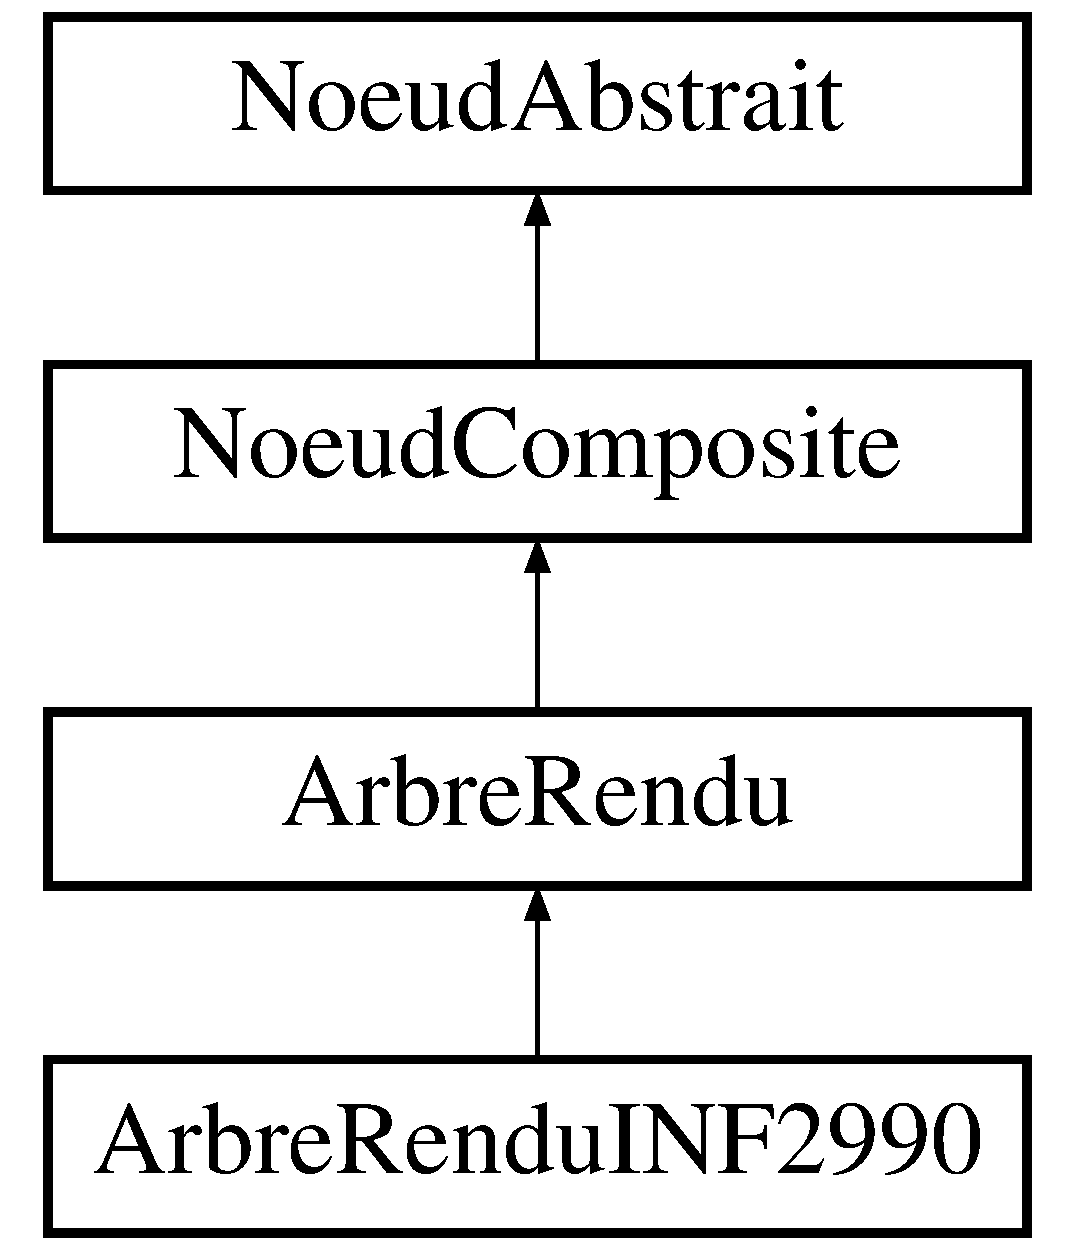
\includegraphics[height=4.000000cm]{class_arbre_rendu}
\end{center}
\end{figure}
\subsection*{Public Member Functions}
\begin{DoxyCompactItemize}
\item 
\hyperlink{group__inf2990_gaef1e98a66c4f1d3b468c786edee45ae6}{Arbre\+Rendu} ()
\begin{DoxyCompactList}\small\item\em Constructeur par d�faut. \end{DoxyCompactList}\item 
virtual \hyperlink{group__inf2990_gadb462923759da0ff632dad097b7bfdab}{$\sim$\+Arbre\+Rendu} ()
\begin{DoxyCompactList}\small\item\em Destructeur. \end{DoxyCompactList}\item 
void \hyperlink{group__inf2990_ga9d6dd6caf1139ae20e998b9bc12e4f88}{ajouter\+Usine} (const std\+::string \&type, std\+::unique\+\_\+ptr$<$ const \hyperlink{class_usine_abstraite}{Usine\+Abstraite} $>$ usine)
\begin{DoxyCompactList}\small\item\em Ajoute une usine associ�e � un type de noeud. \end{DoxyCompactList}\item 
std\+::shared\+\_\+ptr$<$ \hyperlink{class_noeud_abstrait}{Noeud\+Abstrait} $>$ \hyperlink{group__inf2990_ga554972eadae0ba78b0ca5507bb1bde79}{creer\+Noeud} (const std\+::string \&type\+Nouveau\+Noeud) const 
\begin{DoxyCompactList}\small\item\em Cr�e un nouveau noeud. \end{DoxyCompactList}\item 
std\+::shared\+\_\+ptr$<$ \hyperlink{class_noeud_abstrait}{Noeud\+Abstrait} $>$ \hyperlink{group__inf2990_gabc51bdf3355cfa019d7319a484d99c9f}{ajouter\+Nouveau\+Noeud} (const std\+::string \&nom\+Parent, const std\+::string \&type\+Nouveau\+Noeud)
\begin{DoxyCompactList}\small\item\em Cr�e et ajoute un nouveau noeud � l\textquotesingle{}arbre. \end{DoxyCompactList}\item 
void \hyperlink{group__inf2990_ga3a48da8aedbe9ea5f4c183a07e51cbdc}{accepter\+Visiteur} (\hyperlink{class_visiteur_abstrait}{Visiteur\+Abstrait} $\ast$visiteur)
\begin{DoxyCompactList}\small\item\em Accepter un visiteur. \end{DoxyCompactList}\item 
void \hyperlink{group__inf2990_ga35250fdfe013915a44bd17b5e5ed7c93}{assigner\+Chemin\+Fichier\+Zone} (std\+::string chemin)
\begin{DoxyCompactList}\small\item\em Assigne le chemin du fichier s�lectionn� par l\textquotesingle{}utilisateur. \end{DoxyCompactList}\item 
F\+I\+LE $\ast$ \hyperlink{group__inf2990_gadd7c49de3ccb9d5c93d98a524f5a0ca4}{obtenir\+Fichier\+Zone} (std\+::string mode)
\begin{DoxyCompactList}\small\item\em Retourne un pointeur vers le fichier s�lectionn� par l\textquotesingle{}utilisateur. \end{DoxyCompactList}\item 
std\+::string \hyperlink{group__inf2990_ga4aa0f8040fa05c5ecdfed670e1bf908b}{obtenir\+Chemin\+Fichier\+Zone\+Defaut} ()
\begin{DoxyCompactList}\small\item\em Retourne le chemin vers le fichier de zone de base. \end{DoxyCompactList}\end{DoxyCompactItemize}
\subsection*{Static Public Member Functions}
\begin{DoxyCompactItemize}
\item 
static unsigned int \hyperlink{group__inf2990_gacf0e53d52040b07cd6550fda79867bd5}{calculer\+Profondeur\+Maximale} ()
\begin{DoxyCompactList}\small\item\em Calcule la profondeur maximale possible pour l\textquotesingle{}arbre de rendu. \end{DoxyCompactList}\end{DoxyCompactItemize}
\subsection*{Protected Member Functions}
\begin{DoxyCompactItemize}
\item 
F\+I\+LE $\ast$ \hyperlink{group__inf2990_ga3a833324a1b1498d54018dd6b45fba8f}{obtenir\+Fichier\+Zone\+Defaut} (std\+::string mode)
\begin{DoxyCompactList}\small\item\em Retourne un pointeur vers le fichier de structure de base. \end{DoxyCompactList}\end{DoxyCompactItemize}
\subsection*{Protected Attributes}
\begin{DoxyCompactItemize}
\item 
const std\+::string \hyperlink{class_arbre_rendu_a2dc3fd097cae37d9a8cb9d5989b08898}{chemin\+Fichier\+Zone\+Defaut} = \char`\"{}./Zones/zone\+\_\+par\+\_\+defaut.\+json\char`\"{}\hypertarget{class_arbre_rendu_a2dc3fd097cae37d9a8cb9d5989b08898}{}\label{class_arbre_rendu_a2dc3fd097cae37d9a8cb9d5989b08898}

\begin{DoxyCompactList}\small\item\em Constante repr�sentant le fichier zone contenant la structure de base. \end{DoxyCompactList}\item 
std\+::string \hyperlink{class_arbre_rendu_ad8d94407279b476fba573f2c7840e5e0}{chemin\+Fichier\+Zone}\hypertarget{class_arbre_rendu_ad8d94407279b476fba573f2c7840e5e0}{}\label{class_arbre_rendu_ad8d94407279b476fba573f2c7840e5e0}

\begin{DoxyCompactList}\small\item\em Chemin vers le fichier de zone s�lectionn� par l\textquotesingle{}utilisateur. \end{DoxyCompactList}\end{DoxyCompactItemize}
\subsection*{Additional Inherited Members}


\subsection{Detailed Description}
Classe d\textquotesingle{}arbre de rendu qui contient la racine de l\textquotesingle{}arbre de rendu avec les usines qui permettent d\textquotesingle{}ajouter des noeuds � cet arbre. 

La profondeur de cet arbre est limit�e par la taille de la pile des matrices et la taille de la pile des noms pour la s�lection Open\+GL, �tant donn� que chaque niveau de l\textquotesingle{}arbre effectue un \char`\"{}push\char`\"{} sur chacune de ces piles lors du rendu. L\textquotesingle{}arbre ne v�rifie pas que la profondeur reste sous la limite, mais il offre des fonctions permettant de le v�rifier ais�ment.

\begin{DoxyAuthor}{Author}
Martin Bisson 
\end{DoxyAuthor}
\begin{DoxyDate}{Date}
2007-\/01-\/28 
\end{DoxyDate}


The documentation for this class was generated from the following files\+:\begin{DoxyCompactItemize}
\item 
Sources/\+D\+L\+L/\+Arbre/\hyperlink{_arbre_rendu_8h}{Arbre\+Rendu.\+h}\item 
Sources/\+D\+L\+L/\+Arbre/\hyperlink{_arbre_rendu_8cpp}{Arbre\+Rendu.\+cpp}\end{DoxyCompactItemize}

\hypertarget{class_arbre_rendu_i_n_f2990}{}\section{Arbre\+Rendu\+I\+N\+F2990 Class Reference}
\label{class_arbre_rendu_i_n_f2990}\index{Arbre\+Rendu\+I\+N\+F2990@{Arbre\+Rendu\+I\+N\+F2990}}


Classe qui repr�sente l\textquotesingle{}arbre de rendu sp�cifique au projet de I\+N\+F2990.  




{\ttfamily \#include $<$Arbre\+Rendu\+I\+N\+F2990.\+h$>$}

Inheritance diagram for Arbre\+Rendu\+I\+N\+F2990\+:\begin{figure}[H]
\begin{center}
\leavevmode
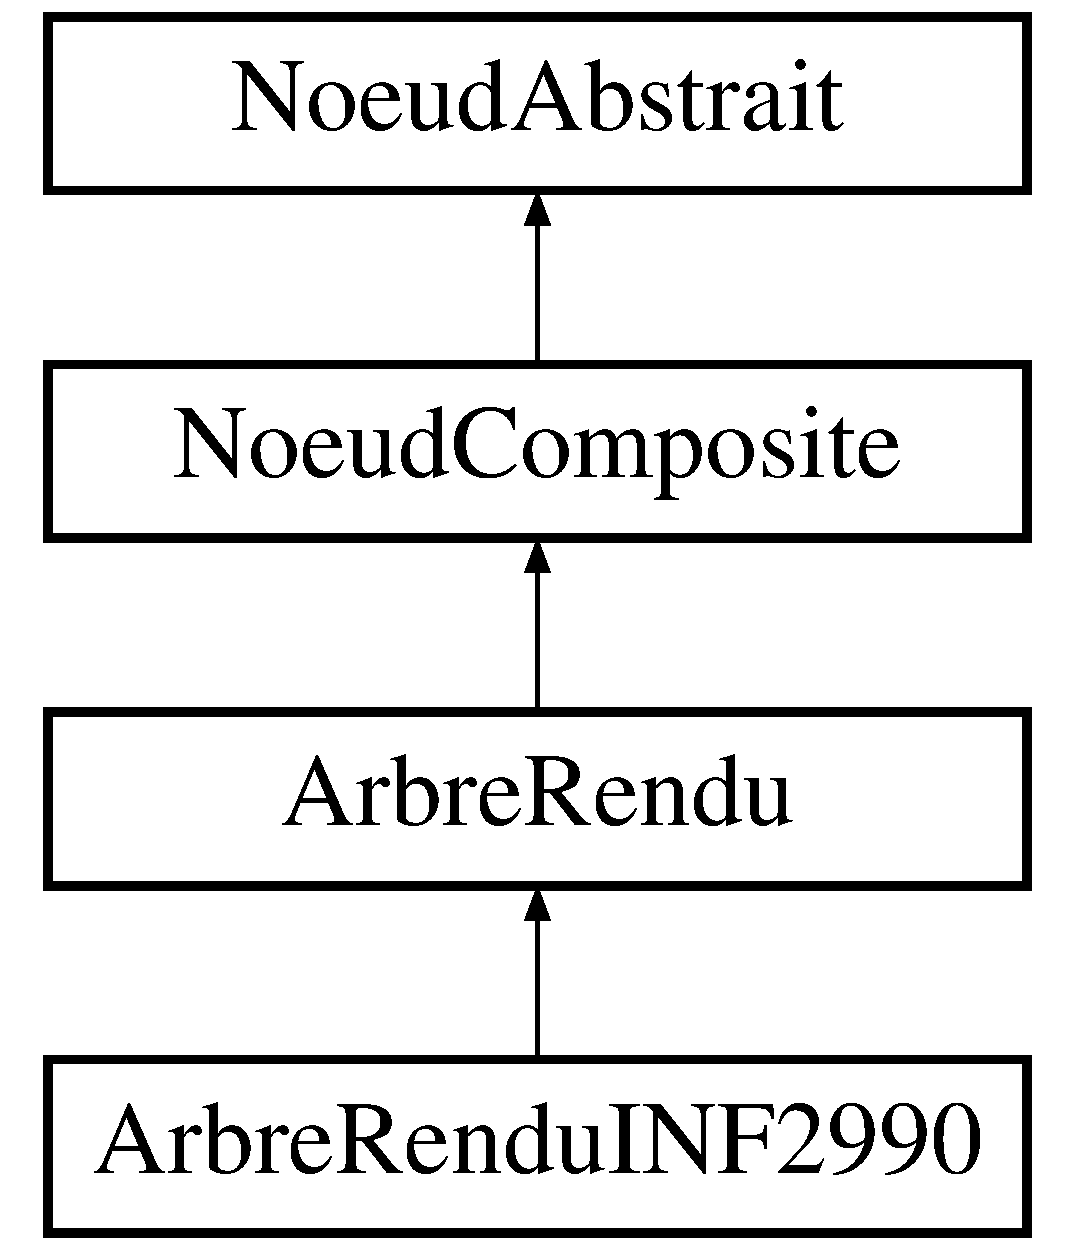
\includegraphics[height=4.000000cm]{class_arbre_rendu_i_n_f2990}
\end{center}
\end{figure}
\subsection*{Public Member Functions}
\begin{DoxyCompactItemize}
\item 
\hyperlink{group__inf2990_ga67528b7fa54e8ef8f96ef2e0bad06d2d}{Arbre\+Rendu\+I\+N\+F2990} ()
\begin{DoxyCompactList}\small\item\em Constructeur par d�faut. \end{DoxyCompactList}\item 
virtual \hyperlink{group__inf2990_gaa67526b2fd719f6bcef7a4547bd25c7b}{$\sim$\+Arbre\+Rendu\+I\+N\+F2990} ()
\begin{DoxyCompactList}\small\item\em Destructeur. \end{DoxyCompactList}\item 
void \hyperlink{group__inf2990_ga678d89e1f12ae16ee7dcf6de3db637a3}{initialiser} ()
\begin{DoxyCompactList}\small\item\em Initialise l\textquotesingle{}arbre de rendu � son �tat initial. \end{DoxyCompactList}\item 
void \hyperlink{group__inf2990_ga9024ef9d92907f74c5068d60734f0296}{charger\+Zone} ()
\begin{DoxyCompactList}\small\item\em Charge le fichier de sauvegarde pr�sentement assign� � l\textquotesingle{}arbre de rendu. \end{DoxyCompactList}\end{DoxyCompactItemize}
\subsection*{Static Public Attributes}
\begin{DoxyCompactItemize}
\item 
static const std\+::string \hyperlink{group__inf2990_ga9a6799aa8903b858929bf675e4468aac}{N\+O\+M\+\_\+\+R\+O\+B\+OT} \{ \char`\"{}robot\char`\"{} \}
\begin{DoxyCompactList}\small\item\em La cha�ne repr�sentant le type du robot. \end{DoxyCompactList}\item 
static const std\+::string \hyperlink{group__inf2990_ga89e651c1a28481ce70f473bd15555114}{N\+O\+M\+\_\+\+T\+A\+B\+LE} \{ \char`\"{}table\char`\"{} \}
\begin{DoxyCompactList}\small\item\em La cha�ne repr�sentant le type de la table. \end{DoxyCompactList}\item 
static const std\+::string \hyperlink{group__inf2990_ga96342d03aed79f57435be49458b49442}{N\+O\+M\+\_\+\+P\+O\+T\+E\+AU} \{ \char`\"{}poteau\char`\"{} \}
\begin{DoxyCompactList}\small\item\em La cha�ne repr�sentant le type des poteaux. \end{DoxyCompactList}\item 
static const std\+::string \hyperlink{group__inf2990_ga4d9c8c9bfa165dde522834dec2882039}{N\+O\+M\+\_\+\+M\+UR} \{ \char`\"{}mur\char`\"{} \}
\begin{DoxyCompactList}\small\item\em La cha�ne repr�sentant le type des murs. \end{DoxyCompactList}\item 
static const std\+::string \hyperlink{group__inf2990_ga7abec330d5b3d29b2ced7bc0c9b85945}{N\+O\+M\+\_\+\+L\+I\+G\+N\+E\+N\+O\+I\+RE} \{ \char`\"{}ligne\+Noire\char`\"{} \}
\begin{DoxyCompactList}\small\item\em La cha�ne repr�sentant le type des lignes. \end{DoxyCompactList}\item 
static const std\+::string \hyperlink{group__inf2990_gaffe953e9369343040aa5d1b72510d810}{N\+O\+M\+\_\+\+S\+E\+G\+M\+E\+NT} \{ \char`\"{}segment\char`\"{} \}
\begin{DoxyCompactList}\small\item\em La cha�ne repr�sentant le type des segments. \end{DoxyCompactList}\item 
static const std\+::string \hyperlink{group__inf2990_ga11612ee8437b54d7d63eb178bbac63dc}{N\+O\+M\+\_\+\+D\+U\+P\+L\+I\+C\+A\+T\+I\+ON} \{ \char`\"{}duplication\char`\"{} \}
\begin{DoxyCompactList}\small\item\em La cha�ne repr�sentant le type des duplications. \end{DoxyCompactList}\item 
static const std\+::string \hyperlink{group__inf2990_ga9905d5dc120cd553b2a1e231456986d6}{N\+O\+M\+\_\+\+J\+O\+N\+C\+T\+I\+ON} \{ \char`\"{}jonction\char`\"{} \}
\begin{DoxyCompactList}\small\item\em La cha�ne repr�sentant le type du point de d�part. \end{DoxyCompactList}\end{DoxyCompactItemize}
\subsection*{Additional Inherited Members}


\subsection{Detailed Description}
Classe qui repr�sente l\textquotesingle{}arbre de rendu sp�cifique au projet de I\+N\+F2990. 

Cette classe s\textquotesingle{}occupe de configurer les usines des noeuds qui seront utilis�s par le projet.

\begin{DoxyAuthor}{Author}
Martin Bisson 
\end{DoxyAuthor}
\begin{DoxyDate}{Date}
2007-\/03-\/23 
\end{DoxyDate}


The documentation for this class was generated from the following files\+:\begin{DoxyCompactItemize}
\item 
Sources/\+D\+L\+L/\+Arbre/\hyperlink{_arbre_rendu_i_n_f2990_8h}{Arbre\+Rendu\+I\+N\+F2990.\+h}\item 
Sources/\+D\+L\+L/\+Arbre/\hyperlink{_arbre_rendu_i_n_f2990_8cpp}{Arbre\+Rendu\+I\+N\+F2990.\+cpp}\end{DoxyCompactItemize}

\hypertarget{class_banc_tests}{}\section{Banc\+Tests Class Reference}
\label{class_banc_tests}\index{Banc\+Tests@{Banc\+Tests}}


Banc de tests qui permet d\textquotesingle{}ex�cuter tous les tests unitaires. C\textquotesingle{}est une classe singleton.  




{\ttfamily \#include $<$Banc\+Tests.\+h$>$}

Inheritance diagram for Banc\+Tests\+:\begin{figure}[H]
\begin{center}
\leavevmode
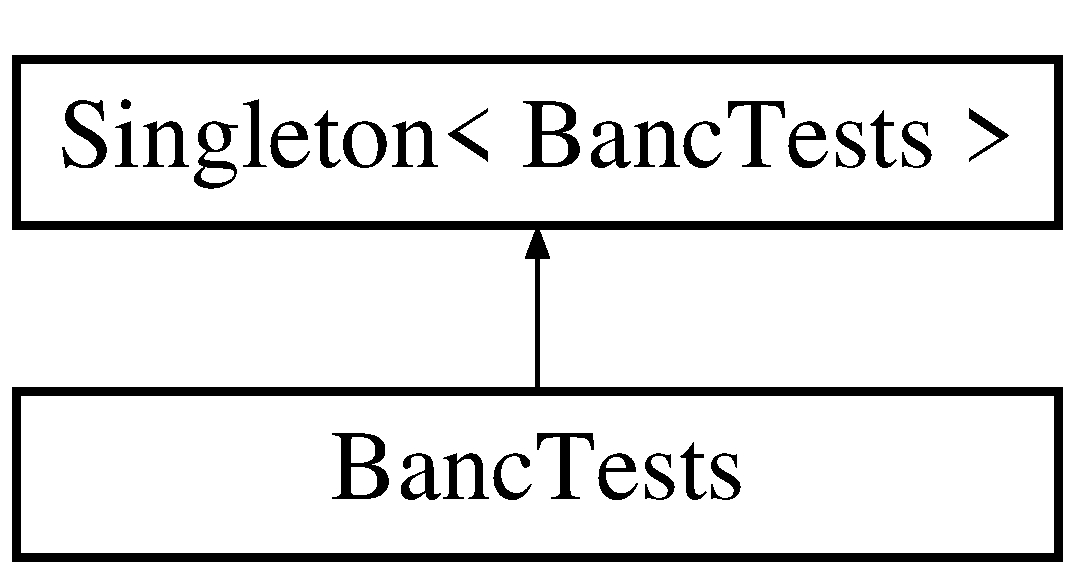
\includegraphics[height=2.000000cm]{class_banc_tests}
\end{center}
\end{figure}
\subsection*{Public Member Functions}
\begin{DoxyCompactItemize}
\item 
bool \hyperlink{group__inf2990_gab5d7fbfe7e3fbe00aa187caa10b1c506}{executer} ()
\begin{DoxyCompactList}\small\item\em Ex�cuter tous les tests unitaires. \end{DoxyCompactList}\end{DoxyCompactItemize}


\subsection{Detailed Description}
Banc de tests qui permet d\textquotesingle{}ex�cuter tous les tests unitaires. C\textquotesingle{}est une classe singleton. 

\begin{DoxyAuthor}{Author}
Julien Gascon-\/\+Samson 
\end{DoxyAuthor}
\begin{DoxyDate}{Date}
2011-\/07-\/16 
\end{DoxyDate}


The documentation for this class was generated from the following files\+:\begin{DoxyCompactItemize}
\item 
Sources/\+D\+L\+L/\+Tests/\hyperlink{_banc_tests_8h}{Banc\+Tests.\+h}\item 
Sources/\+D\+L\+L/\+Tests/\hyperlink{_banc_tests_8cpp}{Banc\+Tests.\+cpp}\end{DoxyCompactItemize}

\hypertarget{class_config_scene}{}\section{Config\+Scene Class Reference}
\label{class_config_scene}\index{Config\+Scene@{Config\+Scene}}


Les variables de configuration de la classe C\+Scene. C\textquotesingle{}est une classe singleton.  




{\ttfamily \#include $<$Config\+Scene.\+h$>$}

Inheritance diagram for Config\+Scene\+:\begin{figure}[H]
\begin{center}
\leavevmode
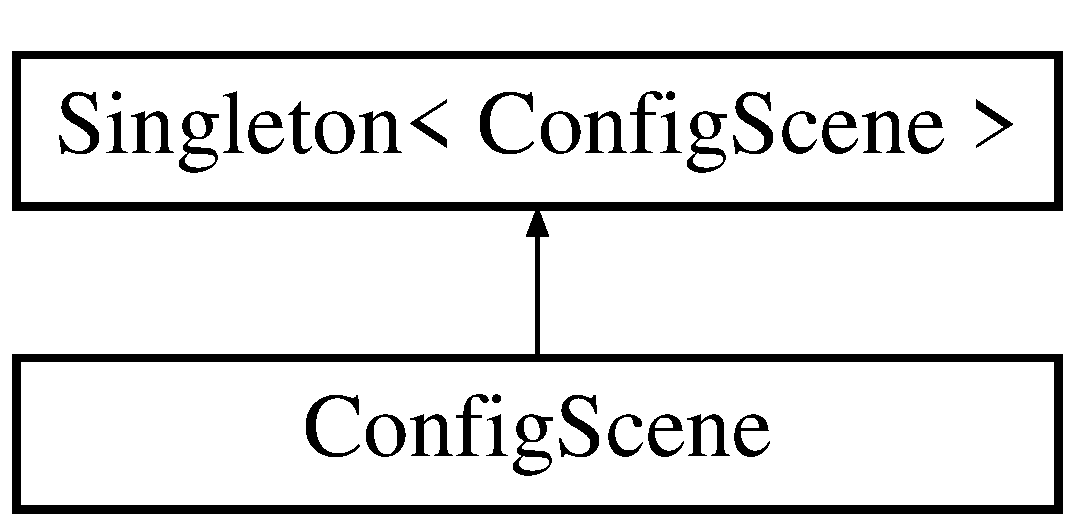
\includegraphics[height=2.000000cm]{class_config_scene}
\end{center}
\end{figure}
\subsection*{Public Member Functions}
\begin{DoxyCompactItemize}
\item 
void \hyperlink{group__inf2990_ga3d0152df0c8c134ecd1a1741302db839}{creer\+D\+OM} (tinyxml2\+::\+X\+M\+L\+Document \&document) const 
\begin{DoxyCompactList}\small\item\em Cr�er le D\+OM avec les valeurs. \end{DoxyCompactList}\item 
void \hyperlink{group__inf2990_gaeacd60be947ce76a1302f6bbb40c90b1}{lire\+D\+OM} (tinyxml2\+::\+X\+M\+L\+Document const \&document)
\begin{DoxyCompactList}\small\item\em Lire les valeurs du D\+OM. \end{DoxyCompactList}\end{DoxyCompactItemize}
\subsection*{Static Public Attributes}
\begin{DoxyCompactItemize}
\item 
static int \hyperlink{group__inf2990_gadb487b450a0314a5d1f75cf31ce502eb}{C\+A\+L\+C\+U\+L\+S\+\_\+\+P\+A\+R\+\_\+\+I\+M\+A\+GE} \{ 50 \}
\begin{DoxyCompactList}\small\item\em Nombre de calculs par image. \end{DoxyCompactList}\end{DoxyCompactItemize}


\subsection{Detailed Description}
Les variables de configuration de la classe C\+Scene. C\textquotesingle{}est une classe singleton. 

\begin{DoxyAuthor}{Author}
Jean-\/\+Fran�ois P�russe 
\end{DoxyAuthor}
\begin{DoxyDate}{Date}
2007-\/01-\/10 
\end{DoxyDate}


The documentation for this class was generated from the following files\+:\begin{DoxyCompactItemize}
\item 
Sources/\+D\+L\+L/\+Configuration/\hyperlink{_config_scene_8h}{Config\+Scene.\+h}\item 
Sources/\+D\+L\+L/\+Configuration/\hyperlink{_config_scene_8cpp}{Config\+Scene.\+cpp}\end{DoxyCompactItemize}

\hypertarget{class_config_scene_test}{}\section{Config\+Scene\+Test Class Reference}
\label{class_config_scene_test}\index{Config\+Scene\+Test@{Config\+Scene\+Test}}


Classe de test cppunit pour tester le bon fonctionnement des m�thodes de la classe \hyperlink{class_config_scene}{Config\+Scene}.  




{\ttfamily \#include $<$Config\+Scene\+Test.\+h$>$}

Inheritance diagram for Config\+Scene\+Test\+:\begin{figure}[H]
\begin{center}
\leavevmode
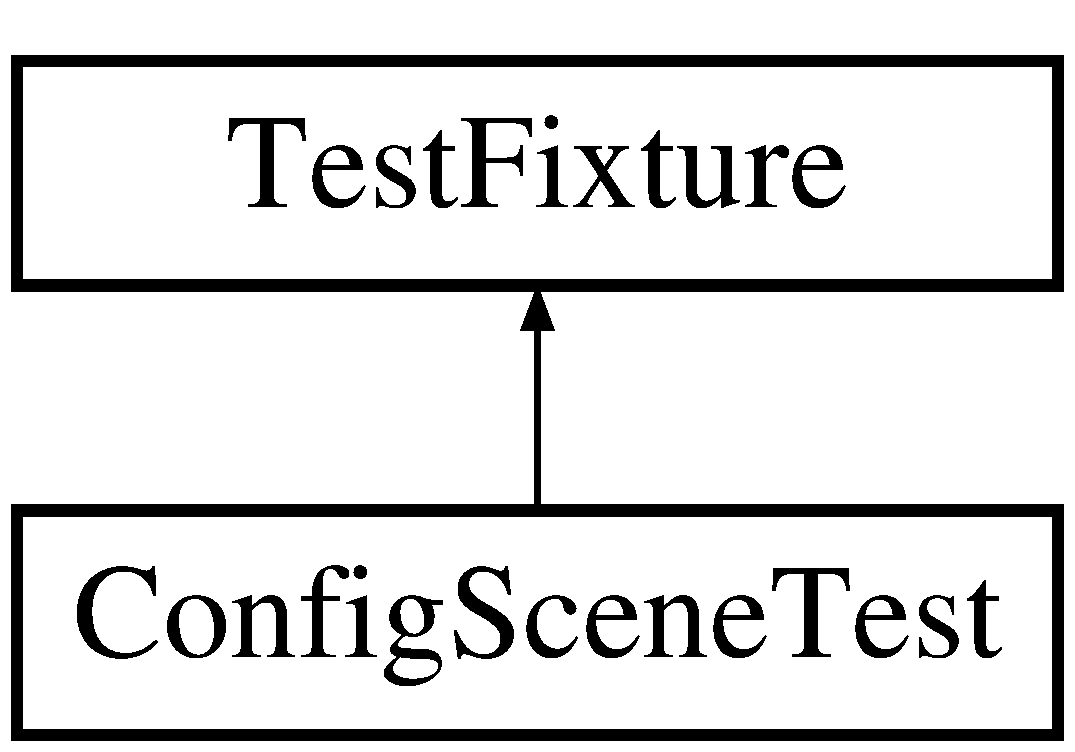
\includegraphics[height=2.000000cm]{class_config_scene_test}
\end{center}
\end{figure}
\subsection*{Public Member Functions}
\begin{DoxyCompactItemize}
\item 
void \hyperlink{group__inf2990_ga707d7400843047e67b736ab79bafb5a0}{set\+Up} ()
\begin{DoxyCompactList}\small\item\em Traitement � effectuer pour initialiser cette suite de tests. \end{DoxyCompactList}\item 
void \hyperlink{group__inf2990_ga889ed3891c3e55280cabb982953906d9}{tear\+Down} ()
\begin{DoxyCompactList}\small\item\em Traitement � effectuer pour \textquotesingle{}finaliser\textquotesingle{} cette suite de tests. \end{DoxyCompactList}\item 
void \hyperlink{group__inf2990_ga0f09d52bc30d87f18b0341e1052efb74}{test\+Sauvegarde\+Chargement} ()
\begin{DoxyCompactList}\small\item\em Cas de test\+: sauvegarde et chargement X\+ML de la configuration. \end{DoxyCompactList}\end{DoxyCompactItemize}


\subsection{Detailed Description}
Classe de test cppunit pour tester le bon fonctionnement des m�thodes de la classe \hyperlink{class_config_scene}{Config\+Scene}. 

\begin{DoxyAuthor}{Author}
Julien Gascon-\/\+Samson 
\end{DoxyAuthor}
\begin{DoxyDate}{Date}
2011-\/07-\/16 
\end{DoxyDate}


The documentation for this class was generated from the following files\+:\begin{DoxyCompactItemize}
\item 
Sources/\+D\+L\+L/\+Tests/\hyperlink{_config_scene_test_8h}{Config\+Scene\+Test.\+h}\item 
Sources/\+D\+L\+L/\+Tests/\hyperlink{_config_scene_test_8cpp}{Config\+Scene\+Test.\+cpp}\end{DoxyCompactItemize}

\hypertarget{class_etat_abstrait}{}\section{Etat\+Abstrait Class Reference}
\label{class_etat_abstrait}\index{Etat\+Abstrait@{Etat\+Abstrait}}


Classe de base pour chaque �tat.  




{\ttfamily \#include $<$Etat\+Abstrait.\+h$>$}

Inheritance diagram for Etat\+Abstrait\+:\begin{figure}[H]
\begin{center}
\leavevmode
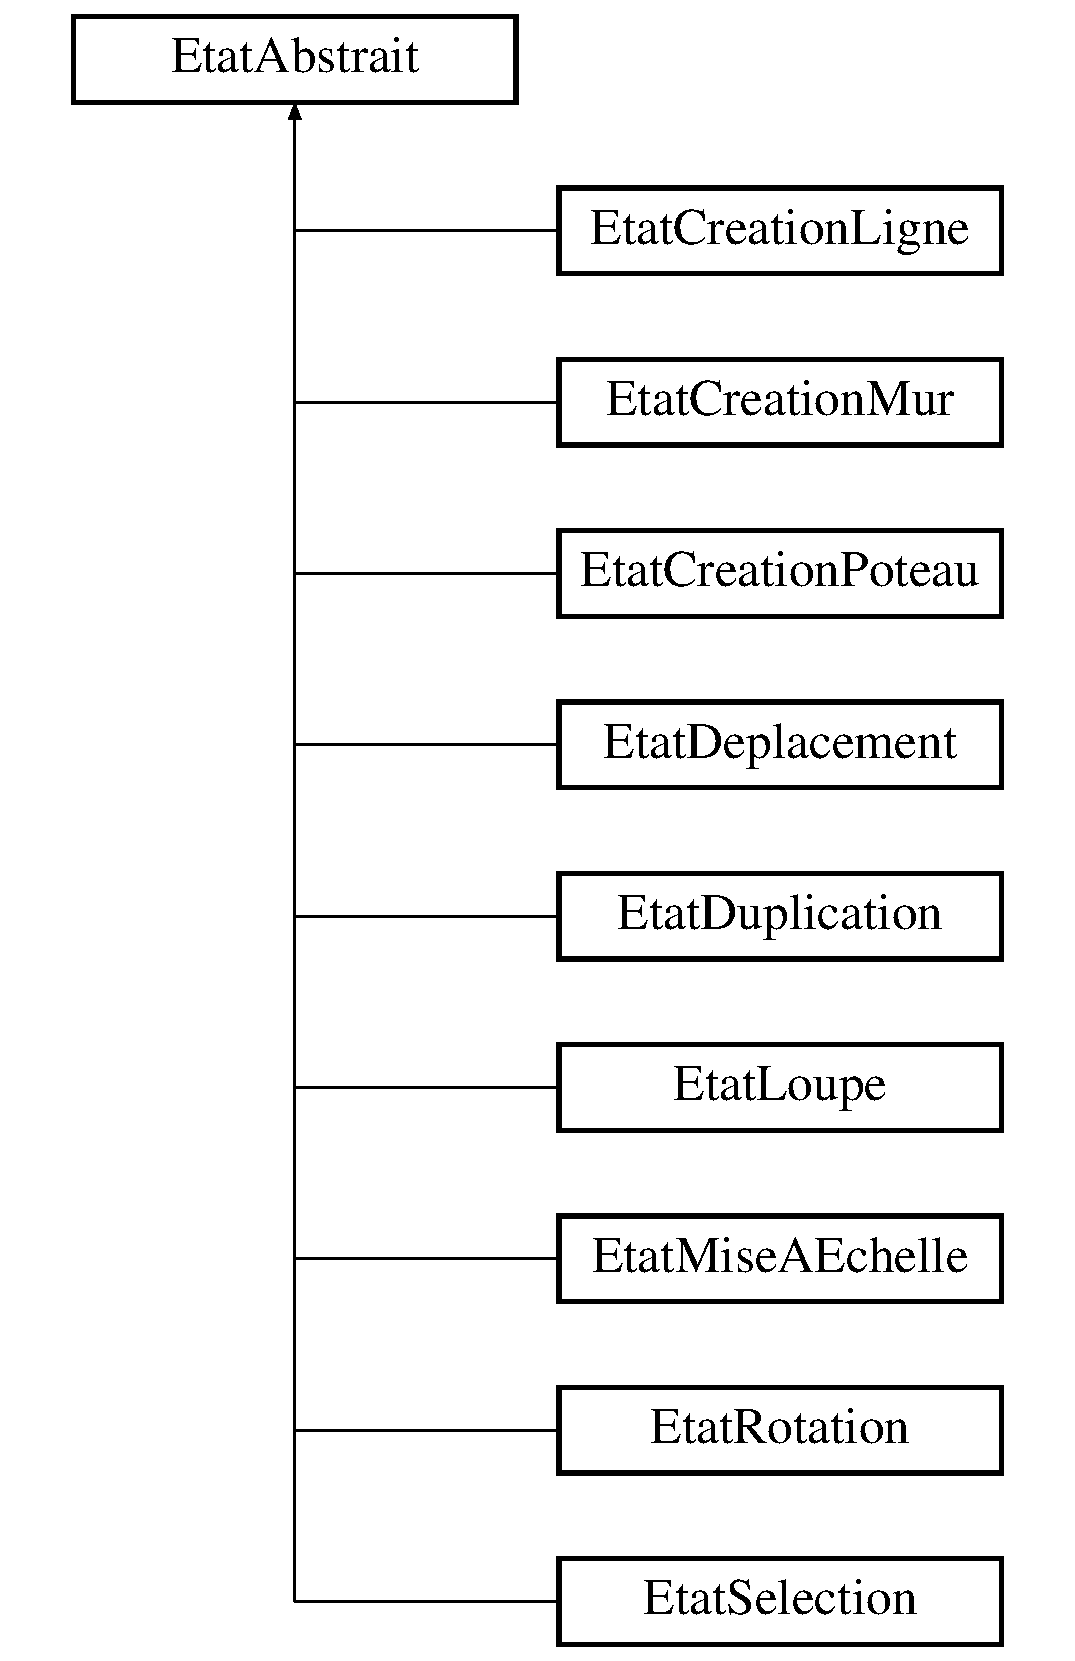
\includegraphics[height=10.000000cm]{class_etat_abstrait}
\end{center}
\end{figure}
\subsection*{Public Member Functions}
\begin{DoxyCompactItemize}
\item 
\hyperlink{group__inf2990_ga9b914f9ecb2481c29747a201fc1a301f}{Etat\+Abstrait} ()
\item 
virtual \hyperlink{group__inf2990_ga1a6172ddf1481cdf211fc00807573a80}{$\sim$\+Etat\+Abstrait} ()
\item 
virtual void \hyperlink{group__inf2990_gab3212ce5e85e1421840bd7815ad56559}{gerer\+Clic\+Droit\+Enfonce} (const int \&x, const int \&y)
\item 
virtual void \hyperlink{group__inf2990_ga82bc3942ed2150f7a6205b1c5f3b23d7}{gerer\+Clic\+Droit\+Relache} (const int \&x, const int \&y)
\item 
virtual void \hyperlink{group__inf2990_ga2fa7ef97df853038f1dbadb87ef5ecb4}{gerer\+Clic\+Gauche\+Enfonce} (const int \&x, const int \&y)
\item 
virtual void \hyperlink{group__inf2990_gaece56739690f25b0a8684c40314b925f}{gerer\+Clic\+Gauche\+Relache} (const int \&x, const int \&y)
\item 
virtual void \hyperlink{group__inf2990_ga07323010436eb82aaea4aa97dc78d22c}{gerer\+Mouvement\+Souris} (const int \&x, const int \&y)
\item 
virtual void \hyperlink{group__inf2990_ga3346dc7c47453f4967163b28ca567582}{gerer\+Molette\+Souris} (const int \&delta)
\item 
void \hyperlink{group__inf2990_gaed414187683d41354b1375e1b66aeab1}{gerer\+Position\+Curseur} (const glm\+::dvec3 \&position)
\item 
virtual void \hyperlink{group__inf2990_gafa83c3ee948b289db3aebb9e9f39b89e}{gerer\+Position\+Curseur\+Concret} (const bool \&pointeur\+Est\+Sur\+Table)
\item 
virtual void \hyperlink{group__inf2990_gae89d06bf5f515c84d614d04544f4251c}{assigner\+Symbole\+Curseur} ()
\item 
virtual void \hyperlink{group__inf2990_ga3dbbaf5f5bbfe9fd95fb04c8ed9a9f66}{gerer\+Touche\+Echappe} ()
\item 
virtual void \hyperlink{group__inf2990_ga931f88a2e4c5f47fb11c0bdff049650c}{gerer\+Touche\+Control\+Enfoncee} ()
\item 
virtual void \hyperlink{group__inf2990_gae316f64de34504e032ac9006c5332223}{gerer\+Touche\+Control\+Relachee} ()
\item 
virtual void \hyperlink{group__inf2990_gac724890a4e60b4ccc2b797f46f5630cf}{gerer\+Touche\+Plus} ()
\item 
virtual void \hyperlink{group__inf2990_ga19f4bf73de9b1d4d5367cf3c4a530344}{gerer\+Touche\+Moins} ()
\item 
virtual void \hyperlink{group__inf2990_ga92b224c1193d057ecf888fee27e5b134}{gerer\+Touche\+Alt\+Enfoncee} ()
\item 
virtual void \hyperlink{group__inf2990_gae24d38b60e87095107acd01656529ec6}{gerer\+Touche\+Alt\+Relachee} ()
\item 
Etat {\bfseries obtenir\+Type\+Etat} () const 
\end{DoxyCompactItemize}
\subsection*{Protected Member Functions}
\begin{DoxyCompactItemize}
\item 
virtual void {\bfseries reinitialiser} ()
\item 
bool \hyperlink{group__inf2990_gac6f990ae9a92441a55a6bc7aca012f10}{est\+Click\+Drag} ()
\end{DoxyCompactItemize}
\subsection*{Protected Attributes}
\begin{DoxyCompactItemize}
\item 
Etat {\bfseries type\+Etat\+\_\+} \{ S\+E\+L\+E\+C\+T\+I\+ON \}\hypertarget{class_etat_abstrait_af9f670d61cc41e2c1abda11520ca2822}{}\label{class_etat_abstrait_af9f670d61cc41e2c1abda11520ca2822}

\item 
\hyperlink{class_arbre_rendu}{Arbre\+Rendu} $\ast$ {\bfseries arbre\+\_\+} \{ nullptr \}\hypertarget{class_etat_abstrait_a85e902c77bc59e7811aaf93b5337a961}{}\label{class_etat_abstrait_a85e902c77bc59e7811aaf93b5337a961}

\item 
vue\+::\+Vue $\ast$ {\bfseries vue\+\_\+} \{ nullptr \}\hypertarget{class_etat_abstrait_ad5cbe2e405407f15195c6969f37c7529}{}\label{class_etat_abstrait_ad5cbe2e405407f15195c6969f37c7529}

\item 
bool {\bfseries curseur\+Est\+Sur\+Table\+\_\+} \{ true \}\hypertarget{class_etat_abstrait_a833619501285048df45f0bc10f27ce58}{}\label{class_etat_abstrait_a833619501285048df45f0bc10f27ce58}

\item 
bool {\bfseries en\+Creation\+\_\+} \{ false \}\hypertarget{class_etat_abstrait_a85caca169aab21d232058cf4fd7513b7}{}\label{class_etat_abstrait_a85caca169aab21d232058cf4fd7513b7}

\item 
bool {\bfseries touche\+Ctrl\+Enfonce\+\_\+} \{ false \}\hypertarget{class_etat_abstrait_a526dc0d0727d4604cfda5dec3ce3f50c}{}\label{class_etat_abstrait_a526dc0d0727d4604cfda5dec3ce3f50c}

\item 
bool {\bfseries touche\+Alt\+Enfonce\+\_\+} \{ false \}\hypertarget{class_etat_abstrait_a5620a3521f0e5b45387a5767882833b6}{}\label{class_etat_abstrait_a5620a3521f0e5b45387a5767882833b6}

\item 
bool {\bfseries clic\+Gauche\+Enfonce\+\_\+} \{false\}\hypertarget{class_etat_abstrait_ae0259dd0b6a86f116464b44fc87bd108}{}\label{class_etat_abstrait_ae0259dd0b6a86f116464b44fc87bd108}

\item 
bool {\bfseries clic\+Droit\+Enfonce\+\_\+} \{false\}\hypertarget{class_etat_abstrait_a53d5538a5e63d01b6453de5d67e84803}{}\label{class_etat_abstrait_a53d5538a5e63d01b6453de5d67e84803}

\item 
int {\bfseries ancien\+X\+\_\+} \{ 0 \}\hypertarget{class_etat_abstrait_a55e1049c0e3e4bbc42abf6b1b5db01ca}{}\label{class_etat_abstrait_a55e1049c0e3e4bbc42abf6b1b5db01ca}

\item 
int {\bfseries ancien\+Y\+\_\+} \{ 0 \}\hypertarget{class_etat_abstrait_a5dbe766e0063c68a96c4865c76353e1d}{}\label{class_etat_abstrait_a5dbe766e0063c68a96c4865c76353e1d}

\item 
glm\+::ivec2 {\bfseries anchor} \{glm\+::ivec2()\}\hypertarget{class_etat_abstrait_aee37db227e8541ef0fcd671a1d2bc05d}{}\label{class_etat_abstrait_aee37db227e8541ef0fcd671a1d2bc05d}

\end{DoxyCompactItemize}
\subsection*{Static Protected Attributes}
\begin{DoxyCompactItemize}
\item 
static glm\+::ivec2 {\bfseries current\+Position\+\_\+} = \{ 0.\+0, 0.\+0 \}
\end{DoxyCompactItemize}


\subsection{Detailed Description}
Classe de base pour chaque �tat. 

Cette classe abstraite comprend l\textquotesingle{}interface de base que doivent implanter tous les �tats pouvant �tre pr�sent dans le mod�le

\begin{DoxyAuthor}{Author}
Fr�d�ric Gr�goire 
\end{DoxyAuthor}
\begin{DoxyDate}{Date}
2016-\/02-\/15 
\end{DoxyDate}


The documentation for this class was generated from the following files\+:\begin{DoxyCompactItemize}
\item 
Sources/\+D\+L\+L/\+Machine\+A\+Etats/\hyperlink{_etat_abstrait_8h}{Etat\+Abstrait.\+h}\item 
Sources/\+D\+L\+L/\+Machine\+A\+Etats/\hyperlink{_etat_abstrait_8cpp}{Etat\+Abstrait.\+cpp}\item 
Sources/\+D\+L\+L/\+Machine\+A\+Etats/Etat\+Creation\+Ligne.\+cpp\item 
Sources/\+D\+L\+L/\+Machine\+A\+Etats/\hyperlink{_etat_creation_mur_8cpp}{Etat\+Creation\+Mur.\+cpp}\item 
Sources/\+D\+L\+L/\+Machine\+A\+Etats/\hyperlink{_etat_creation_poteau_8cpp}{Etat\+Creation\+Poteau.\+cpp}\item 
Sources/\+D\+L\+L/\+Machine\+A\+Etats/\hyperlink{_etat_duplication_8cpp}{Etat\+Duplication.\+cpp}\end{DoxyCompactItemize}

\hypertarget{class_etat_creation_ligne}{}\section{Etat\+Creation\+Ligne Class Reference}
\label{class_etat_creation_ligne}\index{Etat\+Creation\+Ligne@{Etat\+Creation\+Ligne}}


�tat repr�sentant la creation d\textquotesingle{}une ligne.  




{\ttfamily \#include $<$Etat\+Creation\+Ligne.\+h$>$}

Inheritance diagram for Etat\+Creation\+Ligne\+:\begin{figure}[H]
\begin{center}
\leavevmode
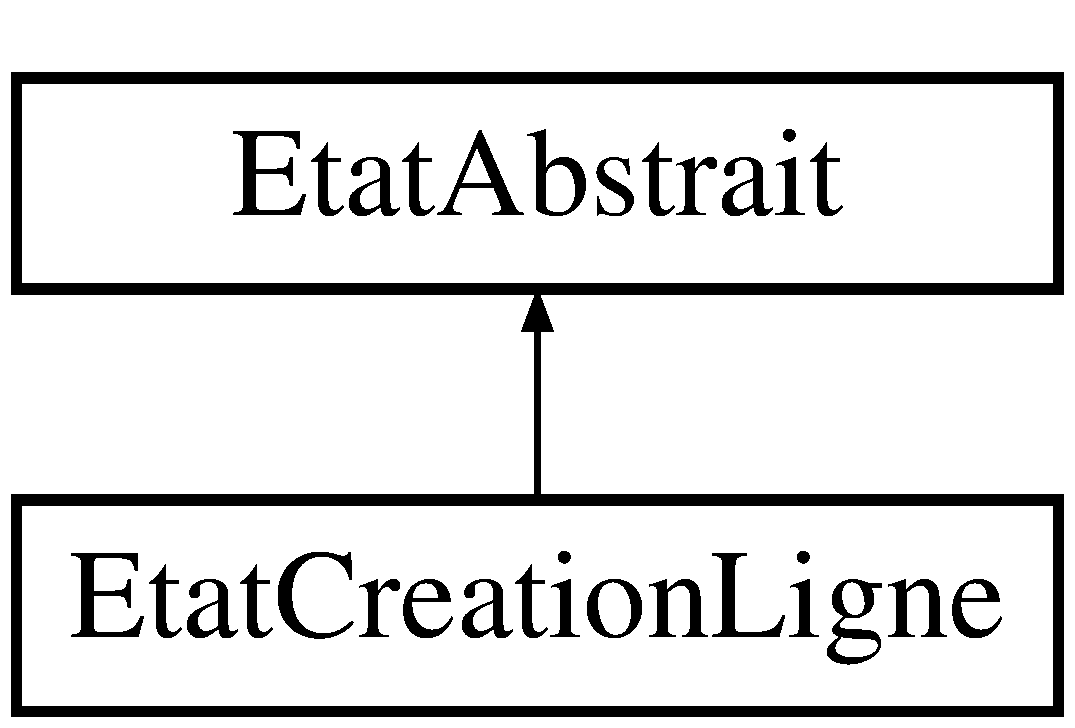
\includegraphics[height=2.000000cm]{class_etat_creation_ligne}
\end{center}
\end{figure}
\subsection*{Public Member Functions}
\begin{DoxyCompactItemize}
\item 
\hyperlink{group__inf2990_gab3c55db445d0ad305a035f37fcb1e238}{Etat\+Creation\+Ligne} ()
\item 
virtual \hyperlink{group__inf2990_ga2b979ae468ab0f6bbc3788fd8ec15bba}{$\sim$\+Etat\+Creation\+Ligne} ()
\item 
virtual void \hyperlink{group__inf2990_ga938704e5f01951d5812adffd54a07bcf}{gerer\+Clic\+Gauche\+Relache} (const int \&x, const int \&y)
\item 
virtual void \hyperlink{group__inf2990_ga3d54cbd509238bea295eee94c0715c37}{gerer\+Mouvement\+Souris} (const int \&x, const int \&y)
\item 
virtual void \hyperlink{group__inf2990_gad01249c2266b7fecb33e768b91626a48}{gerer\+Touche\+Echappe} ()
\item 
virtual void \hyperlink{group__inf2990_ga574018b4c6c81ed1c633c11b45a81411}{gerer\+Touche\+Control\+Enfoncee} ()
\item 
virtual void \hyperlink{group__inf2990_ga9d4a6b853d1f1923c9d506588fc327c1}{gerer\+Touche\+Control\+Relachee} ()
\item 
virtual void \hyperlink{group__inf2990_gaa19958bd12211a17ea700c7df295c9e7}{gerer\+Position\+Curseur\+Concret} (const bool \&position\+Est\+Sur\+Table)
\item 
virtual void \hyperlink{group__inf2990_gaaa63d053209eb19baaa1a4cbb9562839}{assigner\+Symbole\+Curseur} ()
\end{DoxyCompactItemize}
\subsection*{Additional Inherited Members}


\subsection{Detailed Description}
�tat repr�sentant la creation d\textquotesingle{}une ligne. 

\begin{DoxyAuthor}{Author}
Fr�d�ric Gr�goire 
\end{DoxyAuthor}
\begin{DoxyDate}{Date}
2016-\/02-\/15 
\end{DoxyDate}


The documentation for this class was generated from the following files\+:\begin{DoxyCompactItemize}
\item 
Sources/\+D\+L\+L/\+Machine\+A\+Etats/\hyperlink{_etat_creation_ligne_8h}{Etat\+Creation\+Ligne.\+h}\item 
Sources/\+D\+L\+L/\+Machine\+A\+Etats/Etat\+Creation\+Ligne.\+cpp\end{DoxyCompactItemize}

\hypertarget{class_etat_creation_mur}{}\section{Etat\+Creation\+Mur Class Reference}
\label{class_etat_creation_mur}\index{Etat\+Creation\+Mur@{Etat\+Creation\+Mur}}


�tat repr�sentant la creation d\textquotesingle{}un mur.  




{\ttfamily \#include $<$Etat\+Creation\+Mur.\+h$>$}

Inheritance diagram for Etat\+Creation\+Mur\+:\begin{figure}[H]
\begin{center}
\leavevmode
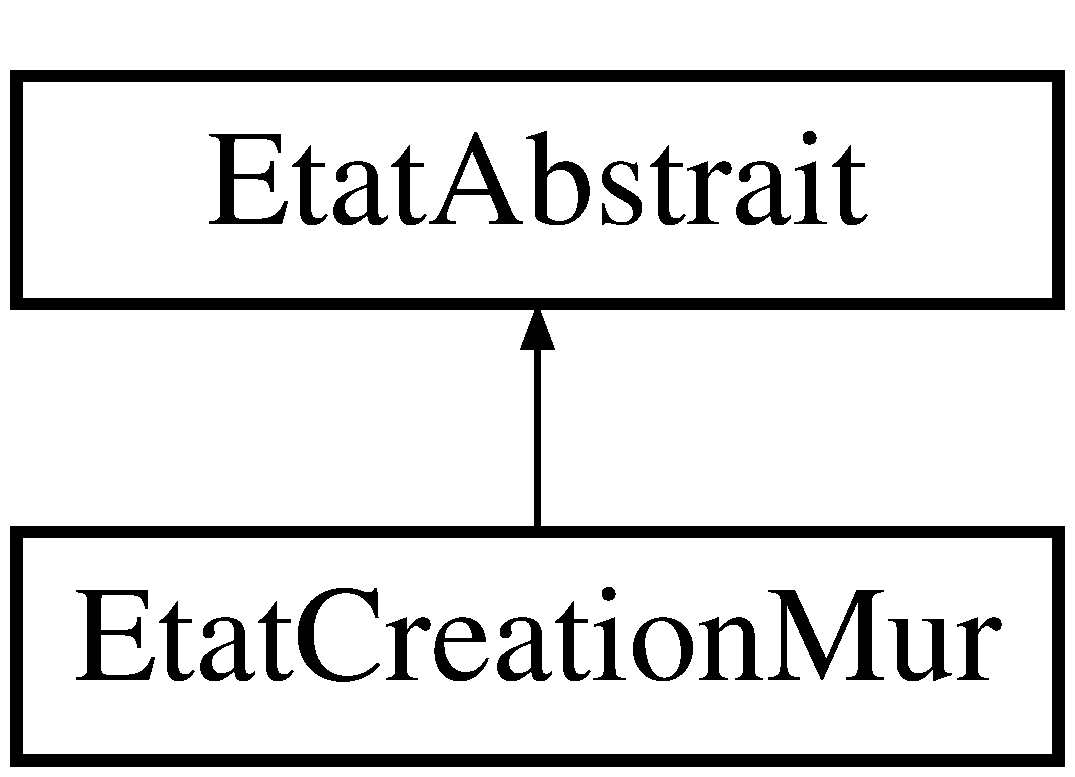
\includegraphics[height=2.000000cm]{class_etat_creation_mur}
\end{center}
\end{figure}
\subsection*{Public Member Functions}
\begin{DoxyCompactItemize}
\item 
\hyperlink{group__inf2990_gabd3123f45a2edd410a49a2daaabbc9d4}{Etat\+Creation\+Mur} ()
\item 
virtual \hyperlink{group__inf2990_ga6d014bfd2831a0847225238c8c331c8d}{$\sim$\+Etat\+Creation\+Mur} ()
\item 
virtual void \hyperlink{group__inf2990_gafb0ca3075883b0a8d39676637934589a}{gerer\+Clic\+Gauche\+Enfonce} (const int \&x, const int \&y)
\item 
virtual void \hyperlink{group__inf2990_gacd606793098ff701c4754f190069852f}{gerer\+Clic\+Gauche\+Relache} (const int \&x, const int \&y)
\item 
virtual void \hyperlink{group__inf2990_ga830e74297eddb366cf88a7594dfd3ee0}{gerer\+Mouvement\+Souris} (const int \&x, const int \&y)
\item 
virtual void \hyperlink{group__inf2990_gab7f11482b50c9dd389647205c3430740}{gerer\+Touche\+Echappe} ()
\item 
virtual void \hyperlink{group__inf2990_ga91825dfb9a438125b8fcc81ff9185162}{gerer\+Position\+Curseur\+Concret} (const bool \&position\+Est\+Sur\+Table)
\item 
virtual void \hyperlink{group__inf2990_ga3fbfd263a90dacab392e07b39f24228f}{assigner\+Symbole\+Curseur} ()
\end{DoxyCompactItemize}
\subsection*{Additional Inherited Members}


\subsection{Detailed Description}
�tat repr�sentant la creation d\textquotesingle{}un mur. 

\begin{DoxyAuthor}{Author}
Fr�d�ric Gr�goire 
\end{DoxyAuthor}
\begin{DoxyDate}{Date}
2016-\/02-\/15 
\end{DoxyDate}


The documentation for this class was generated from the following files\+:\begin{DoxyCompactItemize}
\item 
Sources/\+D\+L\+L/\+Machine\+A\+Etats/\hyperlink{_etat_creation_mur_8h}{Etat\+Creation\+Mur.\+h}\item 
Sources/\+D\+L\+L/\+Machine\+A\+Etats/Etat\+Creation\+Ligne.\+cpp\item 
Sources/\+D\+L\+L/\+Machine\+A\+Etats/\hyperlink{_etat_creation_mur_8cpp}{Etat\+Creation\+Mur.\+cpp}\item 
Sources/\+D\+L\+L/\+Machine\+A\+Etats/\hyperlink{_etat_duplication_8cpp}{Etat\+Duplication.\+cpp}\end{DoxyCompactItemize}

\hypertarget{class_etat_creation_poteau}{}\section{Etat\+Creation\+Poteau Class Reference}
\label{class_etat_creation_poteau}\index{Etat\+Creation\+Poteau@{Etat\+Creation\+Poteau}}


�tat repr�sentant la creation d\textquotesingle{}un poteau.  




{\ttfamily \#include $<$Etat\+Creation\+Poteau.\+h$>$}

Inheritance diagram for Etat\+Creation\+Poteau\+:\begin{figure}[H]
\begin{center}
\leavevmode
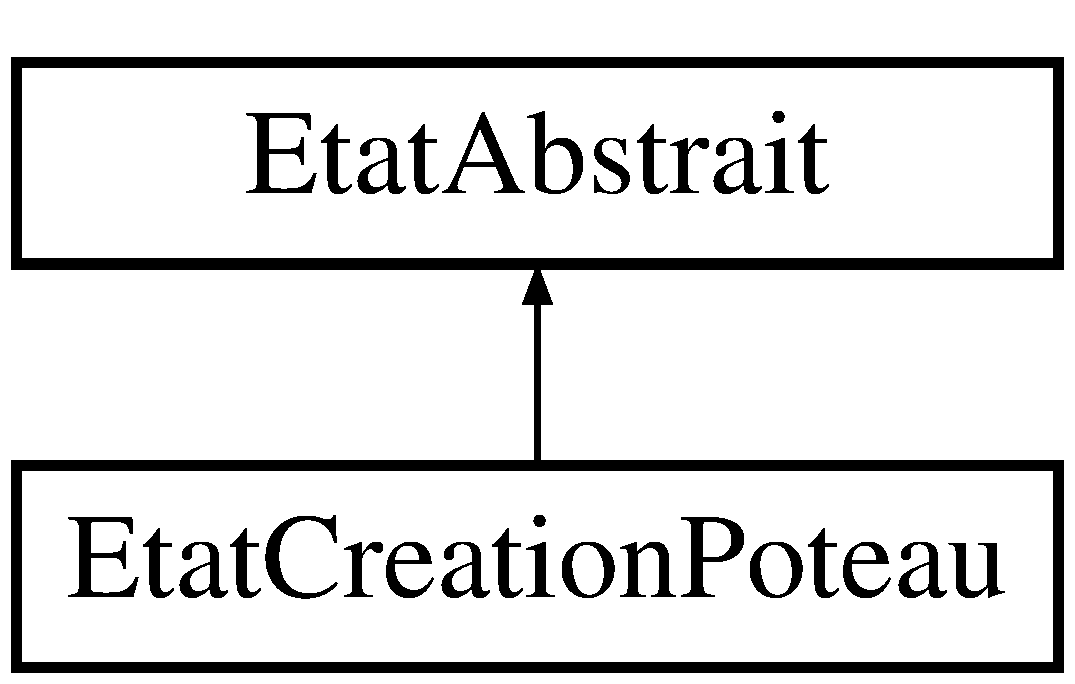
\includegraphics[height=2.000000cm]{class_etat_creation_poteau}
\end{center}
\end{figure}
\subsection*{Public Member Functions}
\begin{DoxyCompactItemize}
\item 
\hyperlink{group__inf2990_ga82c24f7345c525c9ddd96cf9b2e6c024}{Etat\+Creation\+Poteau} ()
\item 
virtual \hyperlink{group__inf2990_gab29874672c8fa38dd6a7a05362ef2ec6}{$\sim$\+Etat\+Creation\+Poteau} ()
\item 
virtual void \hyperlink{group__inf2990_ga6b14f236fddc09008ec4791d53042321}{gerer\+Clic\+Gauche\+Enfonce} (const int \&x, const int \&y)
\item 
virtual void \hyperlink{group__inf2990_ga1253c75e62f62c885aefa826ec98efd7}{gerer\+Clic\+Gauche\+Relache} (const int \&x, const int \&y)
\item 
virtual void \hyperlink{group__inf2990_ga13a7df6614cf35ea625670243d4102a5}{gerer\+Mouvement\+Souris} (const int \&x, const int \&y)
\item 
virtual void \hyperlink{group__inf2990_ga60cb490eeeb2398d75b78eed1c6f9e6a}{gerer\+Position\+Curseur\+Concret} (const bool \&position\+Est\+Sur\+Table)
\item 
virtual void \hyperlink{group__inf2990_ga95b5b867cb109b48afd62276a5f1ba6c}{assigner\+Symbole\+Curseur} ()
\end{DoxyCompactItemize}
\subsection*{Additional Inherited Members}


\subsection{Detailed Description}
�tat repr�sentant la creation d\textquotesingle{}un poteau. 

\begin{DoxyAuthor}{Author}
Fr�d�ric Gr�goire 
\end{DoxyAuthor}
\begin{DoxyDate}{Date}
2016-\/02-\/15 
\end{DoxyDate}


The documentation for this class was generated from the following files\+:\begin{DoxyCompactItemize}
\item 
Sources/\+D\+L\+L/\+Machine\+A\+Etats/\hyperlink{_etat_creation_poteau_8h}{Etat\+Creation\+Poteau.\+h}\item 
Sources/\+D\+L\+L/\+Machine\+A\+Etats/\hyperlink{_etat_creation_poteau_8cpp}{Etat\+Creation\+Poteau.\+cpp}\end{DoxyCompactItemize}

\hypertarget{class_etat_deplacement}{}\section{Etat\+Deplacement Class Reference}
\label{class_etat_deplacement}\index{Etat\+Deplacement@{Etat\+Deplacement}}


�tat repr�sentant le d�placement d\textquotesingle{}un objet.  




{\ttfamily \#include $<$Etat\+Deplacement.\+h$>$}

Inheritance diagram for Etat\+Deplacement\+:\begin{figure}[H]
\begin{center}
\leavevmode
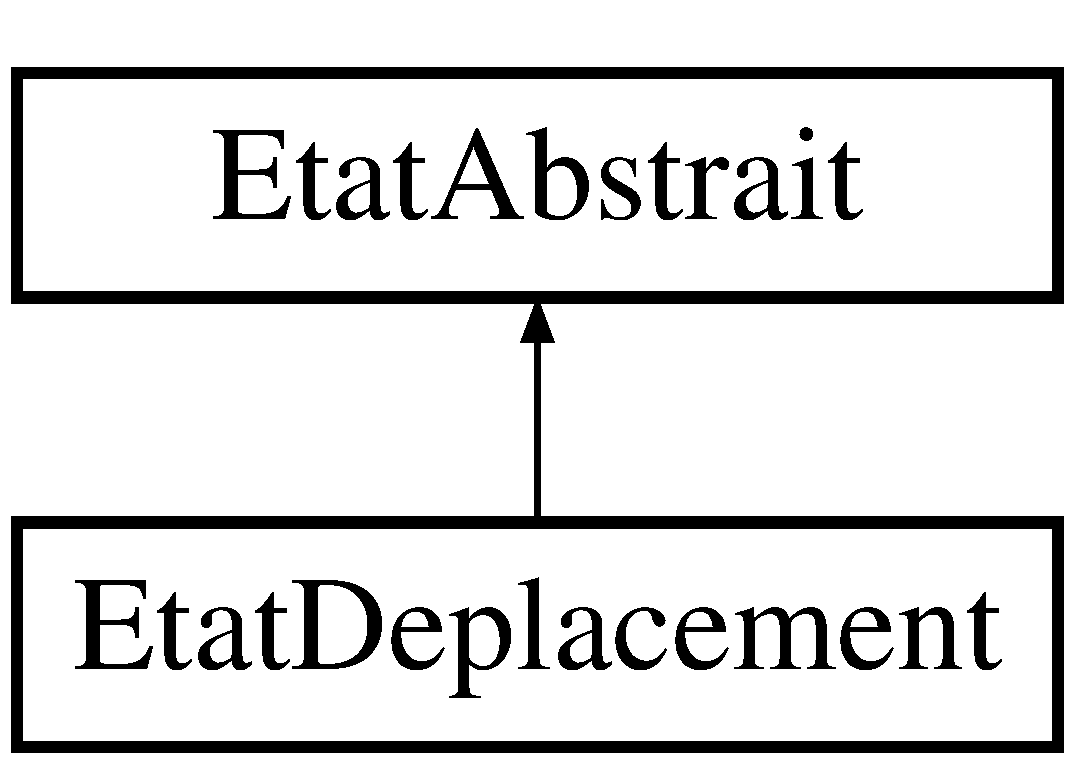
\includegraphics[height=2.000000cm]{class_etat_deplacement}
\end{center}
\end{figure}
\subsection*{Public Member Functions}
\begin{DoxyCompactItemize}
\item 
\hyperlink{group__inf2990_ga42137b0ce81632c647fb74ffe4abcf38}{Etat\+Deplacement} ()
\item 
virtual \hyperlink{group__inf2990_ga6f0bd3c6c3f3808eae0e3c91d6e996a2}{$\sim$\+Etat\+Deplacement} ()
\item 
virtual void \hyperlink{group__inf2990_ga51649f5f8b4792a6ca038c79299036ab}{gerer\+Clic\+Gauche\+Enfonce} (const int \&x, const int \&y)
\item 
virtual void \hyperlink{group__inf2990_gaac738629579c317a0cee4db91199f2a3}{gerer\+Clic\+Gauche\+Relache} (const int \&x, const int \&y)
\item 
virtual void \hyperlink{group__inf2990_ga84924f29c6b9b75902406401c6ad7f6e}{gerer\+Mouvement\+Souris} (const int \&x, const int \&y)
\end{DoxyCompactItemize}
\subsection*{Protected Member Functions}
\begin{DoxyCompactItemize}
\item 
virtual void \hyperlink{group__inf2990_ga86e5267d6d43b28f57ae2c300a0eaacc}{reinitialiser} ()
\end{DoxyCompactItemize}
\subsection*{Additional Inherited Members}


\subsection{Detailed Description}
�tat repr�sentant le d�placement d\textquotesingle{}un objet. 

\begin{DoxyAuthor}{Author}
Fr�d�ric Gr�goire 
\end{DoxyAuthor}
\begin{DoxyDate}{Date}
2016-\/02-\/15 
\end{DoxyDate}


The documentation for this class was generated from the following files\+:\begin{DoxyCompactItemize}
\item 
Sources/\+D\+L\+L/\+Machine\+A\+Etats/\hyperlink{_etat_deplacement_8h}{Etat\+Deplacement.\+h}\item 
Sources/\+D\+L\+L/\+Machine\+A\+Etats/\hyperlink{_etat_deplacement_8cpp}{Etat\+Deplacement.\+cpp}\end{DoxyCompactItemize}

\hypertarget{class_etat_duplication}{}\section{Etat\+Duplication Class Reference}
\label{class_etat_duplication}\index{Etat\+Duplication@{Etat\+Duplication}}


�tat repr�sentant la duplication d\textquotesingle{}un objet.  




{\ttfamily \#include $<$Etat\+Duplication.\+h$>$}

Inheritance diagram for Etat\+Duplication\+:\begin{figure}[H]
\begin{center}
\leavevmode
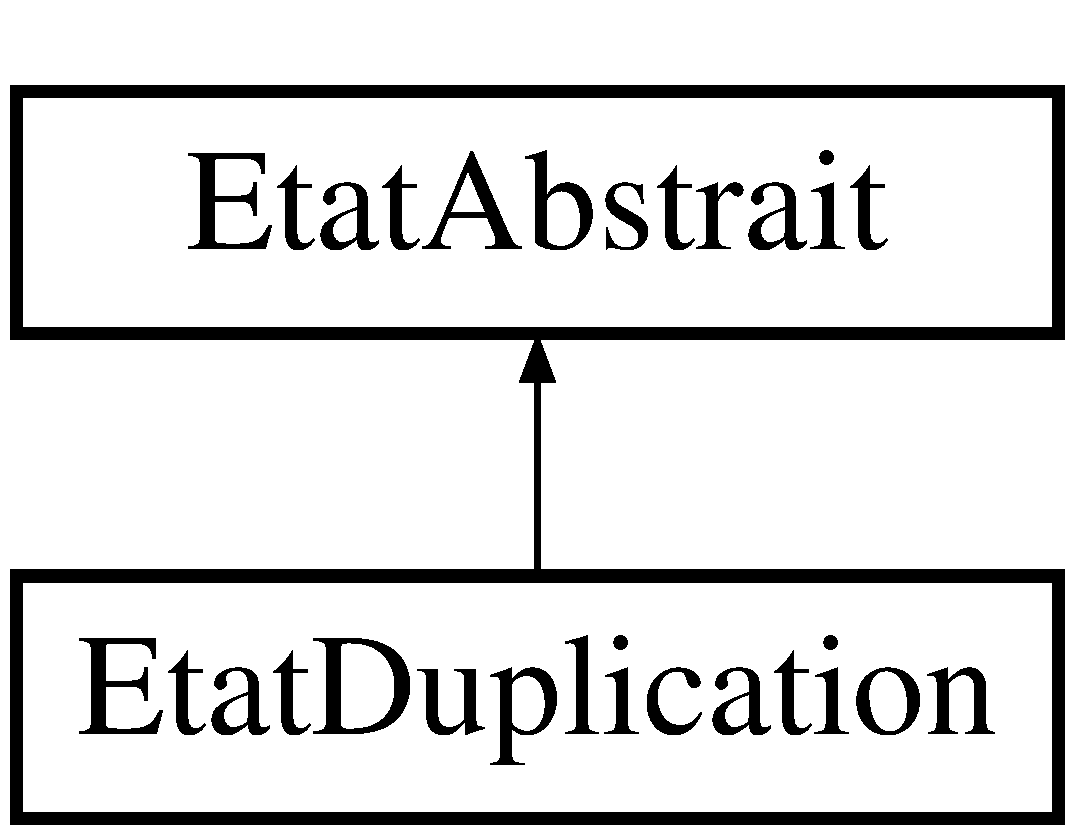
\includegraphics[height=2.000000cm]{class_etat_duplication}
\end{center}
\end{figure}
\subsection*{Public Member Functions}
\begin{DoxyCompactItemize}
\item 
\hyperlink{group__inf2990_ga13ff95bc4765de8d1b7844d8f766fd05}{Etat\+Duplication} ()
\item 
virtual \hyperlink{group__inf2990_ga9fc6f05cae995818d8381c29afaf4099}{$\sim$\+Etat\+Duplication} ()
\item 
virtual void \hyperlink{group__inf2990_gaa29ad7493895057a3059b03c554b0b0c}{gerer\+Clic\+Gauche\+Relache} (const int \&x, const int \&y)
\item 
virtual void \hyperlink{group__inf2990_ga80ba97694a8407056ed1fd4d542d2379}{gerer\+Mouvement\+Souris} (const int \&x, const int \&y)
\item 
virtual void \hyperlink{group__inf2990_ga20dd45a66c7be792451a25254d579606}{gerer\+Position\+Curseur\+Concret} (const bool \&position\+Est\+Sur\+Table)
\item 
virtual void \hyperlink{group__inf2990_gad1bc9bf34d56885243ff95c4f693e252}{assigner\+Symbole\+Curseur} ()
\end{DoxyCompactItemize}
\subsection*{Additional Inherited Members}


\subsection{Detailed Description}
�tat repr�sentant la duplication d\textquotesingle{}un objet. 

\begin{DoxyAuthor}{Author}
Fr�d�ric Gr�goire 
\end{DoxyAuthor}
\begin{DoxyDate}{Date}
2016-\/02-\/15 
\end{DoxyDate}


The documentation for this class was generated from the following files\+:\begin{DoxyCompactItemize}
\item 
Sources/\+D\+L\+L/\+Machine\+A\+Etats/\hyperlink{_etat_duplication_8h}{Etat\+Duplication.\+h}\item 
Sources/\+D\+L\+L/\+Machine\+A\+Etats/\hyperlink{_etat_duplication_8cpp}{Etat\+Duplication.\+cpp}\end{DoxyCompactItemize}

\hypertarget{class_etat_loupe}{}\section{Etat\+Loupe Class Reference}
\label{class_etat_loupe}\index{Etat\+Loupe@{Etat\+Loupe}}


�tat repr�sentant le zoom sur une partie de l\textquotesingle{}�cran.  




{\ttfamily \#include $<$Etat\+Loupe.\+h$>$}

Inheritance diagram for Etat\+Loupe\+:\begin{figure}[H]
\begin{center}
\leavevmode
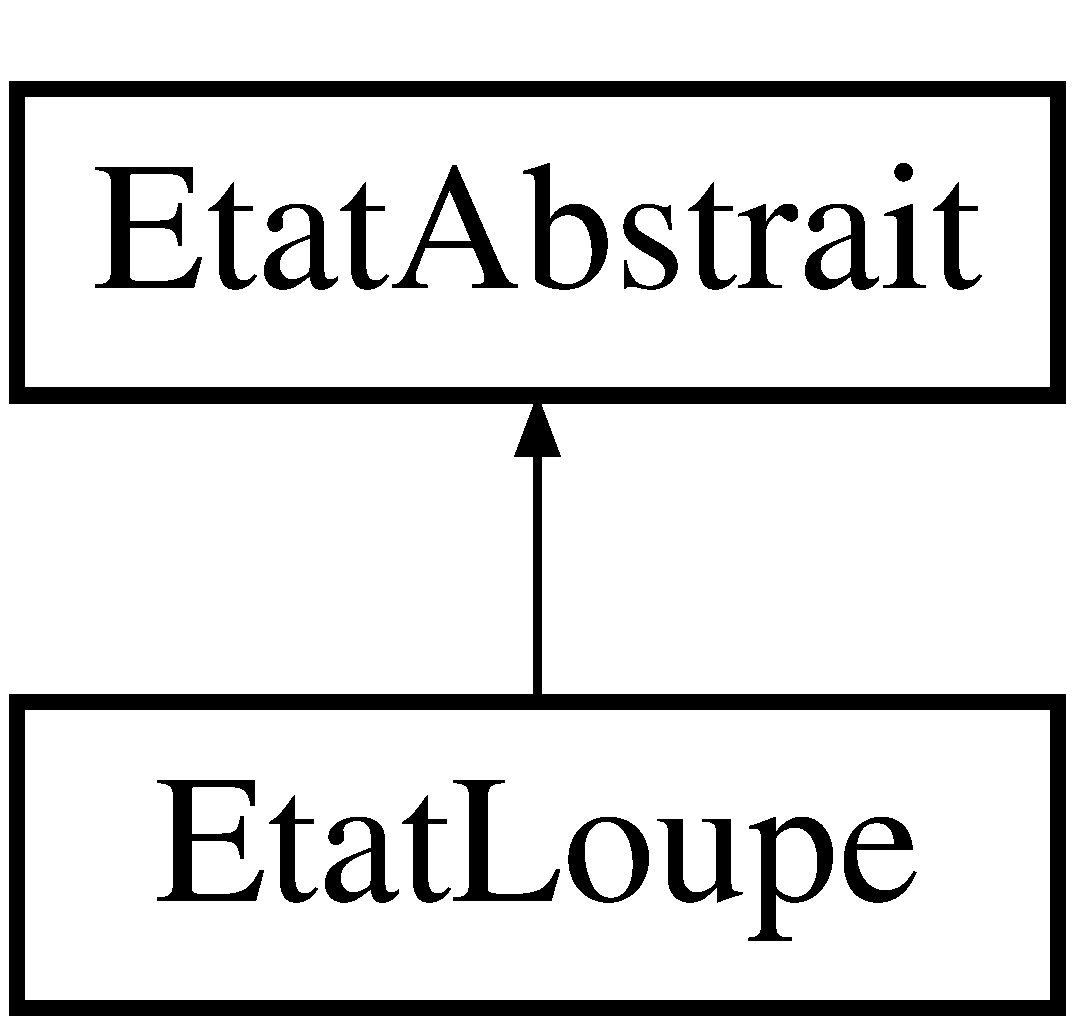
\includegraphics[height=2.000000cm]{class_etat_loupe}
\end{center}
\end{figure}
\subsection*{Public Member Functions}
\begin{DoxyCompactItemize}
\item 
virtual void \hyperlink{group__inf2990_ga171970f0f17de6a4ed3f3536d39da6a2}{gerer\+Clic\+Gauche\+Relache} (const int \&x, const int \&y)
\item 
virtual void \hyperlink{group__inf2990_ga28ab9727d76976b5b88d68ae333a95be}{gerer\+Mouvement\+Souris} (const int \&x, const int \&y)
\end{DoxyCompactItemize}
\subsection*{Additional Inherited Members}


\subsection{Detailed Description}
�tat repr�sentant le zoom sur une partie de l\textquotesingle{}�cran. 

\begin{DoxyAuthor}{Author}
Fr�d�ric Gr�goire 
\end{DoxyAuthor}
\begin{DoxyDate}{Date}
2016-\/02-\/15 
\end{DoxyDate}


The documentation for this class was generated from the following files\+:\begin{DoxyCompactItemize}
\item 
Sources/\+D\+L\+L/\+Machine\+A\+Etats/\hyperlink{_etat_loupe_8h}{Etat\+Loupe.\+h}\item 
Sources/\+D\+L\+L/\+Machine\+A\+Etats/\hyperlink{_etat_loupe_8cpp}{Etat\+Loupe.\+cpp}\end{DoxyCompactItemize}

\hypertarget{class_etat_mise_a_echelle}{}\section{Etat\+Mise\+A\+Echelle Class Reference}
\label{class_etat_mise_a_echelle}\index{Etat\+Mise\+A\+Echelle@{Etat\+Mise\+A\+Echelle}}


�tat repr�sentant la mise � �chelle d\textquotesingle{}un objet.  




{\ttfamily \#include $<$Etat\+Mise\+A\+Echelle.\+h$>$}

Inheritance diagram for Etat\+Mise\+A\+Echelle\+:\begin{figure}[H]
\begin{center}
\leavevmode
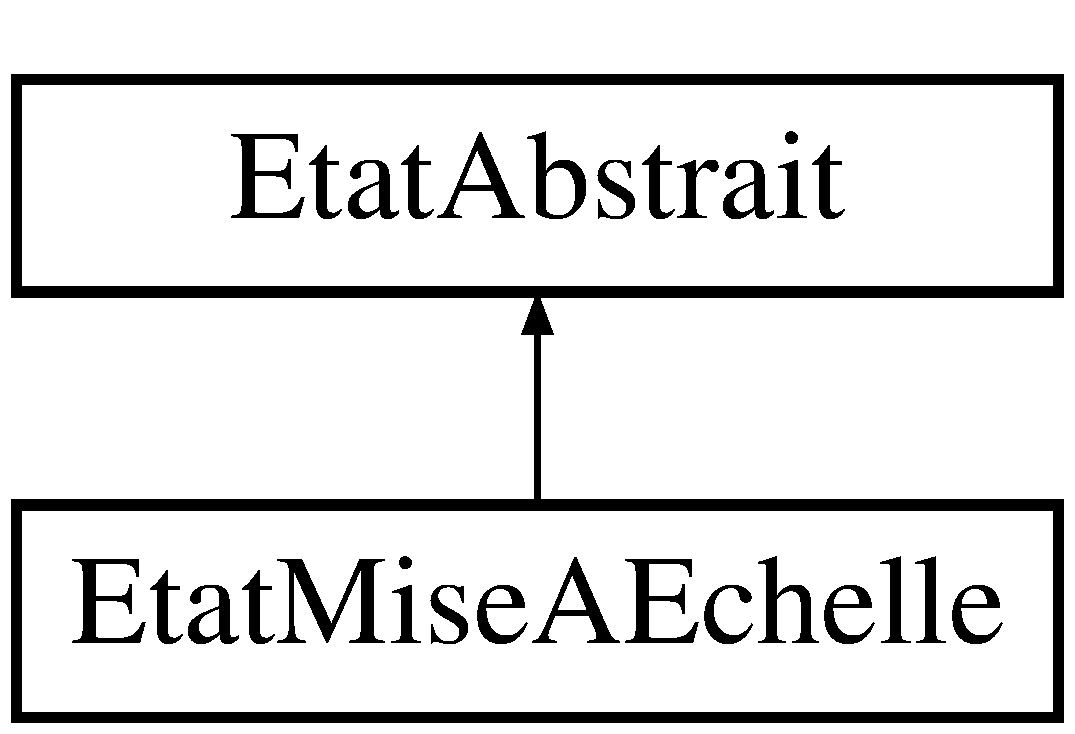
\includegraphics[height=2.000000cm]{class_etat_mise_a_echelle}
\end{center}
\end{figure}
\subsection*{Public Member Functions}
\begin{DoxyCompactItemize}
\item 
\hyperlink{group__inf2990_gabc84ca2d04b82d7278bbfb3c3d1eaafd}{Etat\+Mise\+A\+Echelle} ()
\item 
virtual \hyperlink{group__inf2990_ga29e4617a46653dd23f17e0a2cf64db81}{$\sim$\+Etat\+Mise\+A\+Echelle} ()
\item 
virtual void \hyperlink{group__inf2990_ga80fcd307ff76b42edd932be77bc95529}{gerer\+Clic\+Gauche\+Enfonce} (const int \&x, const int \&y)
\item 
virtual void \hyperlink{group__inf2990_gaa39d323946ed5aacbe90db80d627e3e3}{gerer\+Clic\+Gauche\+Relache} (const int \&x, const int \&y)
\item 
virtual void \hyperlink{group__inf2990_ga142bb4d0433a916980c73dbc710ea788}{gerer\+Mouvement\+Souris} (const int \&x, const int \&y)
\end{DoxyCompactItemize}
\subsection*{Protected Member Functions}
\begin{DoxyCompactItemize}
\item 
virtual void \hyperlink{group__inf2990_gaf188dfff04fd38ec6b17f0037e720298}{reinitialiser} ()
\end{DoxyCompactItemize}
\subsection*{Additional Inherited Members}


\subsection{Detailed Description}
�tat repr�sentant la mise � �chelle d\textquotesingle{}un objet. 

\begin{DoxyAuthor}{Author}
Fr�d�ric Gr�goire 
\end{DoxyAuthor}
\begin{DoxyDate}{Date}
2016-\/02-\/15 
\end{DoxyDate}


The documentation for this class was generated from the following files\+:\begin{DoxyCompactItemize}
\item 
Sources/\+D\+L\+L/\+Machine\+A\+Etats/\hyperlink{_etat_mise_a_echelle_8h}{Etat\+Mise\+A\+Echelle.\+h}\item 
Sources/\+D\+L\+L/\+Machine\+A\+Etats/\hyperlink{_etat_mise_a_echelle_8cpp}{Etat\+Mise\+A\+Echelle.\+cpp}\end{DoxyCompactItemize}

\hypertarget{class_etat_rotation}{}\section{Etat\+Rotation Class Reference}
\label{class_etat_rotation}\index{Etat\+Rotation@{Etat\+Rotation}}


�tat repr�sentant la rotation d\textquotesingle{}un objet.  




{\ttfamily \#include $<$Etat\+Rotation.\+h$>$}

Inheritance diagram for Etat\+Rotation\+:\begin{figure}[H]
\begin{center}
\leavevmode
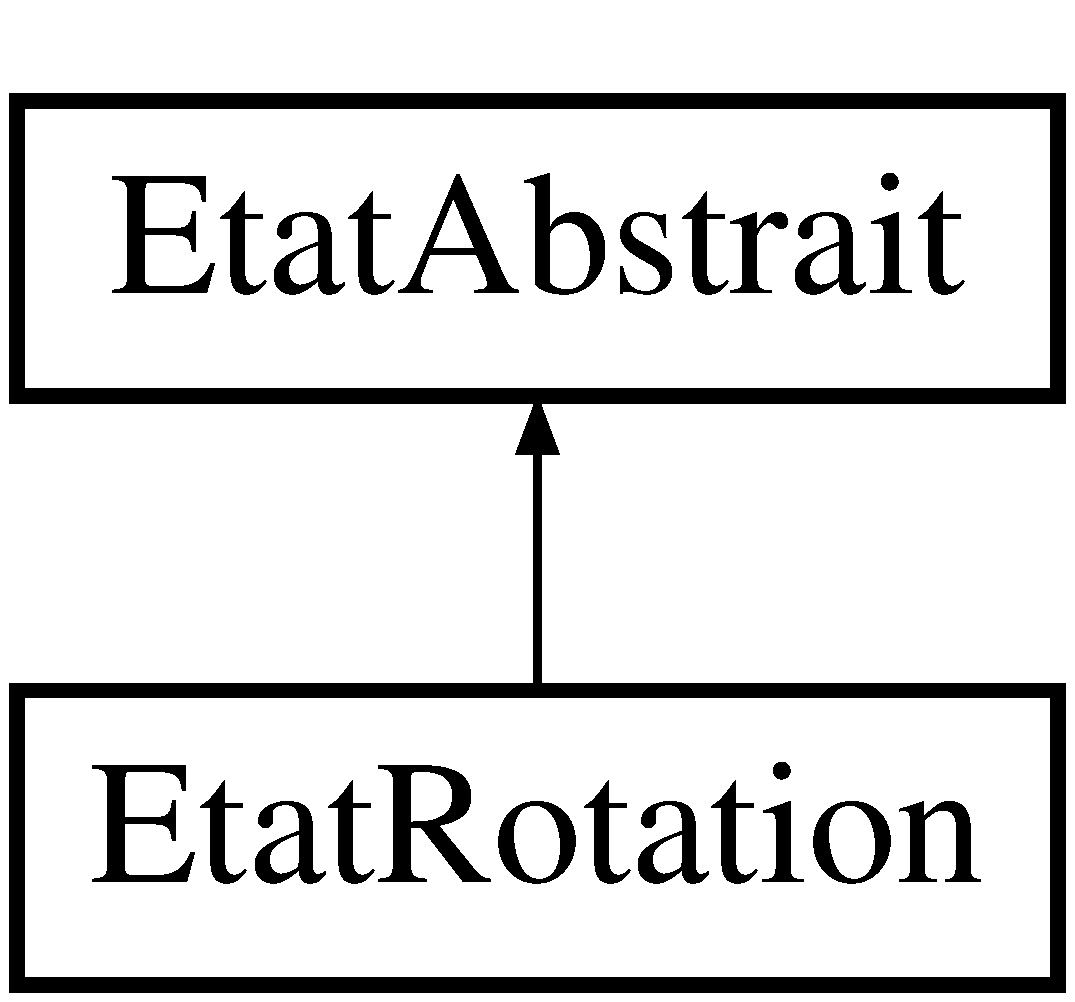
\includegraphics[height=2.000000cm]{class_etat_rotation}
\end{center}
\end{figure}
\subsection*{Public Member Functions}
\begin{DoxyCompactItemize}
\item 
\hyperlink{group__inf2990_gaff6832dd5b77550c48abb138a9dbfe6f}{Etat\+Rotation} ()
\item 
virtual \hyperlink{group__inf2990_ga9da28acc5db46206b400e0ba798b61cc}{$\sim$\+Etat\+Rotation} ()
\item 
virtual void \hyperlink{group__inf2990_ga2b04b7caf55c1424fc973a3cf3872ffe}{gerer\+Clic\+Gauche\+Enfonce} (const int \&x, const int \&y)
\item 
virtual void \hyperlink{group__inf2990_gabd2d95ace041559fc353dbded505e33e}{gerer\+Clic\+Gauche\+Relache} (const int \&x, const int \&y)
\item 
virtual void \hyperlink{group__inf2990_ga0a6e0be7f3ba4925fba6b2348acaf199}{gerer\+Mouvement\+Souris} (const int \&x, const int \&y)
\end{DoxyCompactItemize}
\subsection*{Protected Member Functions}
\begin{DoxyCompactItemize}
\item 
virtual void \hyperlink{group__inf2990_ga0aa3235b22a953fdaf95baa3f130fbe3}{reinitialiser} ()
\end{DoxyCompactItemize}
\subsection*{Additional Inherited Members}


\subsection{Detailed Description}
�tat repr�sentant la rotation d\textquotesingle{}un objet. 

\begin{DoxyAuthor}{Author}
Fr�d�ric Gr�goire 
\end{DoxyAuthor}
\begin{DoxyDate}{Date}
2016-\/02-\/15 
\end{DoxyDate}


The documentation for this class was generated from the following files\+:\begin{DoxyCompactItemize}
\item 
Sources/\+D\+L\+L/\+Machine\+A\+Etats/\hyperlink{_etat_rotation_8h}{Etat\+Rotation.\+h}\item 
Sources/\+D\+L\+L/\+Machine\+A\+Etats/\hyperlink{_etat_rotation_8cpp}{Etat\+Rotation.\+cpp}\end{DoxyCompactItemize}

\hypertarget{class_etat_selection}{}\section{Etat\+Selection Class Reference}
\label{class_etat_selection}\index{Etat\+Selection@{Etat\+Selection}}


�tat repr�sentant la s�lection d\textquotesingle{}un objet.  




{\ttfamily \#include $<$Etat\+Selection.\+h$>$}

Inheritance diagram for Etat\+Selection\+:\begin{figure}[H]
\begin{center}
\leavevmode
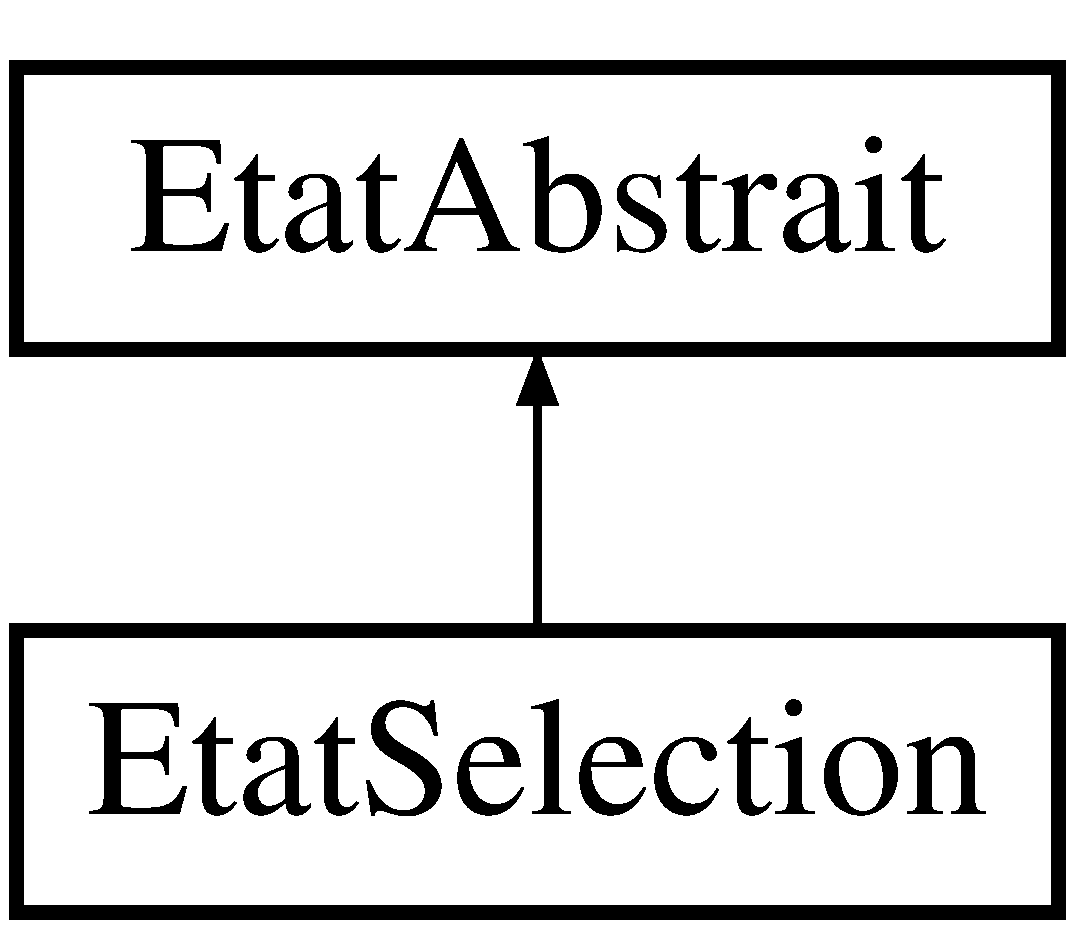
\includegraphics[height=2.000000cm]{class_etat_selection}
\end{center}
\end{figure}
\subsection*{Public Member Functions}
\begin{DoxyCompactItemize}
\item 
\hyperlink{group__inf2990_ga543a303b01da80e3ba9f1cb417612707}{Etat\+Selection} ()
\item 
virtual \hyperlink{group__inf2990_ga0dfa3ac52fdbd9188ee7e348252ad167}{$\sim$\+Etat\+Selection} ()
\item 
virtual void \hyperlink{group__inf2990_ga717efe7a2fa937660862e6313badc87e}{gerer\+Clic\+Gauche\+Relache} (const int \&x, const int \&y)
\item 
virtual void \hyperlink{group__inf2990_ga9ff44503ef87f27631bf5aeb65d17c97}{gerer\+Mouvement\+Souris} (const int \&x, const int \&y)
\item 
void \hyperlink{group__inf2990_ga614bed8e02139fd0fe1138290bb32797}{gerer\+Clic\+Gauche} (const int \&x, const int \&y)
\item 
void \hyperlink{group__inf2990_ga2a4d20fd1ee954878b6d6b0c8e108234}{gerer\+Drag\+Gauche} (const int \&x\+Avant, const int \&y\+Avant, const int \&x\+Apres, const int \&y\+Apres)
\item 
void \hyperlink{group__inf2990_ga99d11e4113dacc57355e8997c88510c8}{gerer\+Touche\+Control\+Enfoncee} ()
\item 
void \hyperlink{group__inf2990_ga9844b3554b04ccb94e4578a40da6c3e4}{gerer\+Touche\+Control\+Relachee} ()
\end{DoxyCompactItemize}
\subsection*{Additional Inherited Members}


\subsection{Detailed Description}
�tat repr�sentant la s�lection d\textquotesingle{}un objet. 

\begin{DoxyAuthor}{Author}
Fr�d�ric Gr�goire 
\end{DoxyAuthor}
\begin{DoxyDate}{Date}
2016-\/02-\/15 
\end{DoxyDate}


The documentation for this class was generated from the following files\+:\begin{DoxyCompactItemize}
\item 
Sources/\+D\+L\+L/\+Machine\+A\+Etats/\hyperlink{_etat_selection_8h}{Etat\+Selection.\+h}\item 
Sources/\+D\+L\+L/\+Machine\+A\+Etats/\hyperlink{_etat_selection_8cpp}{Etat\+Selection.\+cpp}\end{DoxyCompactItemize}

\hypertarget{class_interface_graphique_1_1_explorateur_ouverture}{}\section{Interface\+Graphique.\+Explorateur\+Ouverture Class Reference}
\label{class_interface_graphique_1_1_explorateur_ouverture}\index{Interface\+Graphique.\+Explorateur\+Ouverture@{Interface\+Graphique.\+Explorateur\+Ouverture}}
Inheritance diagram for Interface\+Graphique.\+Explorateur\+Ouverture\+:\begin{figure}[H]
\begin{center}
\leavevmode
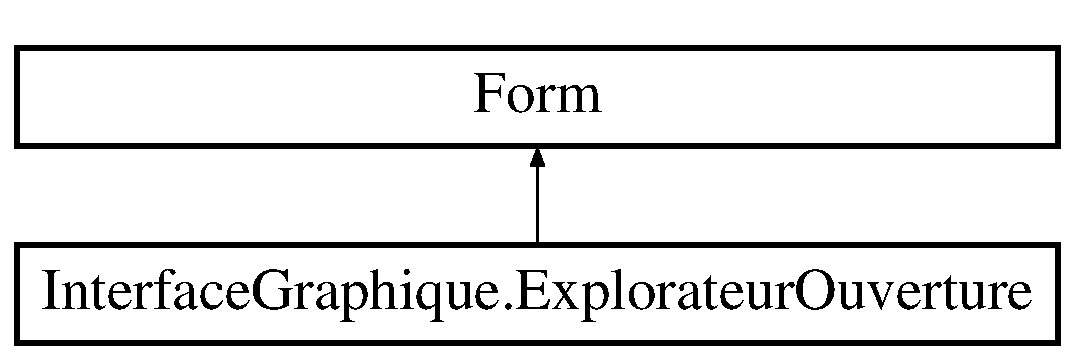
\includegraphics[height=2.000000cm]{class_interface_graphique_1_1_explorateur_ouverture}
\end{center}
\end{figure}
\subsection*{Public Member Functions}
\begin{DoxyCompactItemize}
\item 
\hyperlink{class_interface_graphique_1_1_explorateur_ouverture_a0fb3e86c056c4826c5e3628c88e55102}{Explorateur\+Ouverture} ()
\end{DoxyCompactItemize}
\subsection*{Public Attributes}
\begin{DoxyCompactItemize}
\item 
String \hyperlink{class_interface_graphique_1_1_explorateur_ouverture_a38a03f28bca88334c4b4fb271af7b84e}{chemin\+Fichier}
\begin{DoxyCompactList}\small\item\em Chemin vers le fichier que l\textquotesingle{}utilisateur a sélectionné \end{DoxyCompactList}\end{DoxyCompactItemize}
\subsection*{Protected Member Functions}
\begin{DoxyCompactItemize}
\item 
override void \hyperlink{class_interface_graphique_1_1_explorateur_ouverture_a30f9fd85a97d7db8c0bd0f906684a216}{Dispose} (bool disposing)
\begin{DoxyCompactList}\small\item\em Clean up any resources being used. \end{DoxyCompactList}\end{DoxyCompactItemize}


\subsection{Constructor \& Destructor Documentation}
\index{Interface\+Graphique\+::\+Explorateur\+Ouverture@{Interface\+Graphique\+::\+Explorateur\+Ouverture}!Explorateur\+Ouverture@{Explorateur\+Ouverture}}
\index{Explorateur\+Ouverture@{Explorateur\+Ouverture}!Interface\+Graphique\+::\+Explorateur\+Ouverture@{Interface\+Graphique\+::\+Explorateur\+Ouverture}}
\subsubsection[{\texorpdfstring{Explorateur\+Ouverture()}{ExplorateurOuverture()}}]{\setlength{\rightskip}{0pt plus 5cm}public Interface\+Graphique.\+Explorateur\+Ouverture.\+Explorateur\+Ouverture (
\begin{DoxyParamCaption}
{}
\end{DoxyParamCaption}
)\hspace{0.3cm}{\ttfamily [inline]}}\hypertarget{class_interface_graphique_1_1_explorateur_ouverture_a0fb3e86c056c4826c5e3628c88e55102}{}\label{class_interface_graphique_1_1_explorateur_ouverture_a0fb3e86c056c4826c5e3628c88e55102}
Constructeur par défaut Initialise les composantes du formulaires et popule l\textquotesingle{}arbre de dossiers.

\begin{DoxyReturn}{Returns}
Aucune 
\end{DoxyReturn}


\subsection{Member Function Documentation}
\index{Interface\+Graphique\+::\+Explorateur\+Ouverture@{Interface\+Graphique\+::\+Explorateur\+Ouverture}!Dispose@{Dispose}}
\index{Dispose@{Dispose}!Interface\+Graphique\+::\+Explorateur\+Ouverture@{Interface\+Graphique\+::\+Explorateur\+Ouverture}}
\subsubsection[{\texorpdfstring{Dispose(bool disposing)}{Dispose(bool disposing)}}]{\setlength{\rightskip}{0pt plus 5cm}override void Interface\+Graphique.\+Explorateur\+Ouverture.\+Dispose (
\begin{DoxyParamCaption}
\item[{bool}]{disposing}
\end{DoxyParamCaption}
)\hspace{0.3cm}{\ttfamily [inline]}, {\ttfamily [protected]}}\hypertarget{class_interface_graphique_1_1_explorateur_ouverture_a30f9fd85a97d7db8c0bd0f906684a216}{}\label{class_interface_graphique_1_1_explorateur_ouverture_a30f9fd85a97d7db8c0bd0f906684a216}


Clean up any resources being used. 


\begin{DoxyParams}{Parameters}
{\em disposing} & true if managed resources should be disposed; otherwise, false.\\
\hline
\end{DoxyParams}


\subsection{Member Data Documentation}
\index{Interface\+Graphique\+::\+Explorateur\+Ouverture@{Interface\+Graphique\+::\+Explorateur\+Ouverture}!chemin\+Fichier@{chemin\+Fichier}}
\index{chemin\+Fichier@{chemin\+Fichier}!Interface\+Graphique\+::\+Explorateur\+Ouverture@{Interface\+Graphique\+::\+Explorateur\+Ouverture}}
\subsubsection[{\texorpdfstring{chemin\+Fichier}{cheminFichier}}]{\setlength{\rightskip}{0pt plus 5cm}String Interface\+Graphique.\+Explorateur\+Ouverture.\+chemin\+Fichier}\hypertarget{class_interface_graphique_1_1_explorateur_ouverture_a38a03f28bca88334c4b4fb271af7b84e}{}\label{class_interface_graphique_1_1_explorateur_ouverture_a38a03f28bca88334c4b4fb271af7b84e}


Chemin vers le fichier que l\textquotesingle{}utilisateur a sélectionné 



The documentation for this class was generated from the following files\+:\begin{DoxyCompactItemize}
\item 
Sources/\+Interface\+Graphique/\+Formulaires\+Sys\+Fichiers/Explorateur\+Ouverture.\+cs\item 
Sources/\+Interface\+Graphique/\+Formulaires\+Sys\+Fichiers/Explorateur\+Ouverture.\+Designer.\+cs\end{DoxyCompactItemize}

\hypertarget{class_interface_graphique_1_1_explorateur_sauvegarde}{}\section{Interface\+Graphique.\+Explorateur\+Sauvegarde Class Reference}
\label{class_interface_graphique_1_1_explorateur_sauvegarde}\index{Interface\+Graphique.\+Explorateur\+Sauvegarde@{Interface\+Graphique.\+Explorateur\+Sauvegarde}}


Formulaire permettant à l\textquotesingle{}utilisateur de choisir ou créer dans quel fichier sauvegarder la zone qu\textquotesingle{}il a créée.  


Inheritance diagram for Interface\+Graphique.\+Explorateur\+Sauvegarde\+:\begin{figure}[H]
\begin{center}
\leavevmode
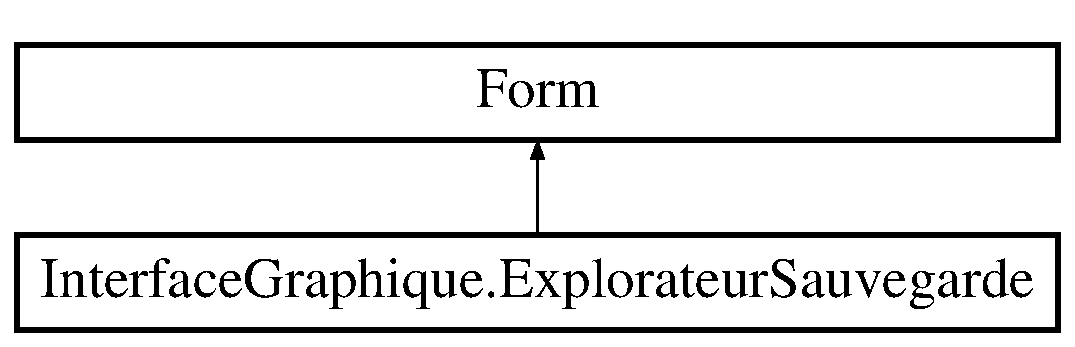
\includegraphics[height=2.000000cm]{class_interface_graphique_1_1_explorateur_sauvegarde}
\end{center}
\end{figure}
\subsection*{Public Member Functions}
\begin{DoxyCompactItemize}
\item 
\hyperlink{class_interface_graphique_1_1_explorateur_sauvegarde_aa99675f3c4c62c4f2d73dd919c38ceb6}{Explorateur\+Sauvegarde} ()
\end{DoxyCompactItemize}
\subsection*{Public Attributes}
\begin{DoxyCompactItemize}
\item 
String \hyperlink{class_interface_graphique_1_1_explorateur_sauvegarde_a26064d4364197660043ffa2016318273}{chemin\+Fichier}
\begin{DoxyCompactList}\small\item\em Chemin vers le fichier que l\textquotesingle{}utilisateur a sélectionné \end{DoxyCompactList}\end{DoxyCompactItemize}
\subsection*{Protected Member Functions}
\begin{DoxyCompactItemize}
\item 
override void \hyperlink{class_interface_graphique_1_1_explorateur_sauvegarde_a8bd0e83efca364be374e3ed7935ef46c}{Dispose} (bool disposing)
\begin{DoxyCompactList}\small\item\em Clean up any resources being used. \end{DoxyCompactList}\end{DoxyCompactItemize}


\subsection{Detailed Description}
Formulaire permettant à l\textquotesingle{}utilisateur de choisir ou créer dans quel fichier sauvegarder la zone qu\textquotesingle{}il a créée. 

\begin{DoxyAuthor}{Author}
Philippe Marcotte 
\end{DoxyAuthor}
\begin{DoxyDate}{Date}
2016-\/2-\/13 
\end{DoxyDate}


\subsection{Constructor \& Destructor Documentation}
\index{Interface\+Graphique\+::\+Explorateur\+Sauvegarde@{Interface\+Graphique\+::\+Explorateur\+Sauvegarde}!Explorateur\+Sauvegarde@{Explorateur\+Sauvegarde}}
\index{Explorateur\+Sauvegarde@{Explorateur\+Sauvegarde}!Interface\+Graphique\+::\+Explorateur\+Sauvegarde@{Interface\+Graphique\+::\+Explorateur\+Sauvegarde}}
\subsubsection[{\texorpdfstring{Explorateur\+Sauvegarde()}{ExplorateurSauvegarde()}}]{\setlength{\rightskip}{0pt plus 5cm}public Interface\+Graphique.\+Explorateur\+Sauvegarde.\+Explorateur\+Sauvegarde (
\begin{DoxyParamCaption}
{}
\end{DoxyParamCaption}
)\hspace{0.3cm}{\ttfamily [inline]}}\hypertarget{class_interface_graphique_1_1_explorateur_sauvegarde_aa99675f3c4c62c4f2d73dd919c38ceb6}{}\label{class_interface_graphique_1_1_explorateur_sauvegarde_aa99675f3c4c62c4f2d73dd919c38ceb6}
Constructeur par défaut Initialise les composantes du formulaires et popule l\textquotesingle{}arbre de dossiers.

\begin{DoxyReturn}{Returns}
Aucune 
\end{DoxyReturn}


\subsection{Member Function Documentation}
\index{Interface\+Graphique\+::\+Explorateur\+Sauvegarde@{Interface\+Graphique\+::\+Explorateur\+Sauvegarde}!Dispose@{Dispose}}
\index{Dispose@{Dispose}!Interface\+Graphique\+::\+Explorateur\+Sauvegarde@{Interface\+Graphique\+::\+Explorateur\+Sauvegarde}}
\subsubsection[{\texorpdfstring{Dispose(bool disposing)}{Dispose(bool disposing)}}]{\setlength{\rightskip}{0pt plus 5cm}override void Interface\+Graphique.\+Explorateur\+Sauvegarde.\+Dispose (
\begin{DoxyParamCaption}
\item[{bool}]{disposing}
\end{DoxyParamCaption}
)\hspace{0.3cm}{\ttfamily [inline]}, {\ttfamily [protected]}}\hypertarget{class_interface_graphique_1_1_explorateur_sauvegarde_a8bd0e83efca364be374e3ed7935ef46c}{}\label{class_interface_graphique_1_1_explorateur_sauvegarde_a8bd0e83efca364be374e3ed7935ef46c}


Clean up any resources being used. 


\begin{DoxyParams}{Parameters}
{\em disposing} & true if managed resources should be disposed; otherwise, false.\\
\hline
\end{DoxyParams}


\subsection{Member Data Documentation}
\index{Interface\+Graphique\+::\+Explorateur\+Sauvegarde@{Interface\+Graphique\+::\+Explorateur\+Sauvegarde}!chemin\+Fichier@{chemin\+Fichier}}
\index{chemin\+Fichier@{chemin\+Fichier}!Interface\+Graphique\+::\+Explorateur\+Sauvegarde@{Interface\+Graphique\+::\+Explorateur\+Sauvegarde}}
\subsubsection[{\texorpdfstring{chemin\+Fichier}{cheminFichier}}]{\setlength{\rightskip}{0pt plus 5cm}String Interface\+Graphique.\+Explorateur\+Sauvegarde.\+chemin\+Fichier}\hypertarget{class_interface_graphique_1_1_explorateur_sauvegarde_a26064d4364197660043ffa2016318273}{}\label{class_interface_graphique_1_1_explorateur_sauvegarde_a26064d4364197660043ffa2016318273}


Chemin vers le fichier que l\textquotesingle{}utilisateur a sélectionné 



The documentation for this class was generated from the following files\+:\begin{DoxyCompactItemize}
\item 
Sources/\+Interface\+Graphique/\+Formulaires\+Sys\+Fichiers/\hyperlink{_explorateur_sauvegarde_8cs}{Explorateur\+Sauvegarde.\+cs}\item 
Sources/\+Interface\+Graphique/\+Formulaires\+Sys\+Fichiers/Explorateur\+Sauvegarde.\+Designer.\+cs\end{DoxyCompactItemize}

\hypertarget{class_facade_modele}{}\section{Facade\+Modele Class Reference}
\label{class_facade_modele}\index{Facade\+Modele@{Facade\+Modele}}


Classe qui constitue une interface (une fa�ade) sur l\textquotesingle{}ensemble du mod�le et des classes qui le composent.  




{\ttfamily \#include $<$Facade\+Modele.\+h$>$}

\subsection*{Public Member Functions}
\begin{DoxyCompactItemize}
\item 
\hyperlink{group__inf2990_gad27e80f0e1f2bcbd11abe36cf50497cb}{$\sim$\+Facade\+Modele} ()
\begin{DoxyCompactList}\small\item\em Destructeur. \end{DoxyCompactList}\item 
void \hyperlink{group__inf2990_gabf12ccafbabf1049cb8327cf78699a1b}{initialiser\+Open\+GL} (H\+W\+ND h\+Wnd)
\begin{DoxyCompactList}\small\item\em Cr�e un contexte Open\+GL et initialise celui-\/ci. \end{DoxyCompactList}\item 
void \hyperlink{group__inf2990_ga4967547e0683bfdca700118df1c18bca}{charger\+Configuration} () const 
\begin{DoxyCompactList}\small\item\em Charge la configuration � partir d\textquotesingle{}un fichier X\+ML. \end{DoxyCompactList}\item 
void \hyperlink{group__inf2990_ga277d8d9cea21e20fb366a0d48525f2c9}{enregistrer\+Configuration} () const 
\begin{DoxyCompactList}\small\item\em Enregistre la configuration courante dans un fichier X\+ML. \end{DoxyCompactList}\item 
void \hyperlink{group__inf2990_gac7b831ce13626514e9637c4533d7c15d}{liberer\+Open\+GL} ()
\begin{DoxyCompactList}\small\item\em Lib�re le contexte Open\+GL. \end{DoxyCompactList}\item 
void \hyperlink{group__inf2990_gac884e818dab5fe049a37b3f6f1c5d8c6}{afficher} () const 
\begin{DoxyCompactList}\small\item\em Affiche le contenu du mod�le. \end{DoxyCompactList}\item 
void \hyperlink{group__inf2990_ga23bed5e3b226e446cfee30084150f7f7}{afficher\+Base} () const 
\begin{DoxyCompactList}\small\item\em Affiche la base du contenu du mod�le. \end{DoxyCompactList}\item 
void \hyperlink{group__inf2990_gac57fa53751a72f6e7bb6103ac6aef13e}{assigner\+Etat} (Etat etat)
\begin{DoxyCompactList}\small\item\em Modifie l\textquotesingle{}etat courant. \end{DoxyCompactList}\item 
\hyperlink{class_etat_abstrait}{Etat\+Abstrait} $\ast$ \hyperlink{group__inf2990_gaba4491fee6dc3a741e70ba5d38c4150a}{obtenir\+Etat} ()
\item 
void \hyperlink{group__inf2990_ga37b2fefcf895431ff7b6ce60763cd595}{assigner\+Mode} (Mode mode)
\begin{DoxyCompactList}\small\item\em Modifie l\textquotesingle{}etat courant. \end{DoxyCompactList}\item 
\hyperlink{class_mode_abstrait}{Mode\+Abstrait} $\ast$ \hyperlink{group__inf2990_gabd08d6e066c4e82d721976c5b8983801}{obtenir\+Mode} ()
\item 
int \hyperlink{group__inf2990_gac57319a76756a4c2bf7da299f20bf12f}{obtenir\+Nombre\+Selection} ()
\item 
bool {\bfseries obtenir\+Autorisation\+Input\+Souris} () const 
\item 
void {\bfseries assigner\+Autorisation\+Input\+Souris} (const bool \&autorisation)
\item 
bool {\bfseries obtenir\+Autorisation\+Input\+Clavier} () const 
\item 
void {\bfseries assigner\+Autorisation\+Input\+Clavier} (const bool \&autorisation)
\item 
double \hyperlink{group__inf2990_gad60c637fcf21d9278a78cb53afdf857b}{obtenir\+Angle\+Rotation} ()
\item 
double {\bfseries obtenir\+Facteur\+Mise\+A\+Echelle} ()
\item 
double \hyperlink{group__inf2990_ga7a89072370661808c54006961f45c072}{obtenir\+Position\+RelativeX} ()
\item 
double \hyperlink{group__inf2990_ga43e3b89e1a16eacd03570d4cb2fb9dd0}{obtenir\+Position\+RelativeY} ()
\item 
void \hyperlink{group__inf2990_ga3ee17405ead2f60ff80c440d9b2d36c7}{assigner\+Angle\+Rotation} (const double \&angle)
\item 
void {\bfseries assigner\+Facteur\+Mise\+A\+Echelle} (const double \&facteur\+Mise\+A\+Echelle)
\item 
void \hyperlink{group__inf2990_ga9142fed411fc847584017b419bc9576a}{assigner\+Position\+RelativeX} (const double \&position\+RelativeX)
\item 
void \hyperlink{group__inf2990_ga490588ee2934050306a526f81c09db50}{assigner\+Position\+RelativeY} (const double \&position\+RelativeY)
\item 
vue\+::\+Vue $\ast$ \hyperlink{group__inf2990_gaa56cf96b7e381e0f14e2c9a55be913bf}{obtenir\+Vue} ()
\begin{DoxyCompactList}\small\item\em Retourne la vue courante. \end{DoxyCompactList}\item 
\hyperlink{class_arbre_rendu_i_n_f2990}{Arbre\+Rendu\+I\+N\+F2990} $\ast$ \hyperlink{group__inf2990_gab3577b8dc7cbd9eb04af75a5a5620fab}{obtenir\+Arbre\+Rendu\+I\+N\+F2990} () const 
\begin{DoxyCompactList}\small\item\em Retourne l\textquotesingle{}arbre de rendu. \end{DoxyCompactList}\item 
\hyperlink{class_arbre_rendu_i_n_f2990}{Arbre\+Rendu\+I\+N\+F2990} $\ast$ \hyperlink{group__inf2990_ga12d5594db6a9507b24c7e1ffcd6751af}{obtenir\+Arbre\+Rendu\+I\+N\+F2990} ()
\begin{DoxyCompactList}\small\item\em Retourne l\textquotesingle{}arbre de rendu. \end{DoxyCompactList}\item 
void \hyperlink{group__inf2990_ga4c2a991fe2297e44eeee0de111fb08d2}{reinitialiser} ()
\begin{DoxyCompactList}\small\item\em R�initialise la sc�ne. \end{DoxyCompactList}\item 
void \hyperlink{group__inf2990_ga24dcb4e32cf104797158b398bafbfbb7}{animer} (float temps)
\begin{DoxyCompactList}\small\item\em Anime la sc�ne. \end{DoxyCompactList}\item 
void \hyperlink{group__inf2990_ga54d4ccc521ad8744009999b7b07f36db}{stop\+Affichage} ()
\item 
void \hyperlink{group__inf2990_gac82abe61c32c702d94b5efbaed4dc7f0}{continuer\+Affichage} ()
\end{DoxyCompactItemize}
\subsection*{Static Public Member Functions}
\begin{DoxyCompactItemize}
\item 
static \hyperlink{class_facade_modele}{Facade\+Modele} $\ast$ \hyperlink{group__inf2990_gaf52e6d65d1a911d3e1699fc30af97d38}{obtenir\+Instance} ()
\begin{DoxyCompactList}\small\item\em Obtient l\textquotesingle{}instance unique de la classe. \end{DoxyCompactList}\item 
static void \hyperlink{group__inf2990_gacbf0495fda26f5be37089470dc5f4372}{liberer\+Instance} ()
\begin{DoxyCompactList}\small\item\em Lib�re l\textquotesingle{}instance unique de la classe. \end{DoxyCompactList}\end{DoxyCompactItemize}


\subsection{Detailed Description}
Classe qui constitue une interface (une fa�ade) sur l\textquotesingle{}ensemble du mod�le et des classes qui le composent. 

\begin{DoxyAuthor}{Author}
Martin Bisson 
\end{DoxyAuthor}
\begin{DoxyDate}{Date}
2007-\/02-\/20 
\end{DoxyDate}


The documentation for this class was generated from the following files\+:\begin{DoxyCompactItemize}
\item 
Sources/\+D\+L\+L/\+Application/\hyperlink{_facade_modele_8h}{Facade\+Modele.\+h}\item 
Sources/\+D\+L\+L/\+Application/\hyperlink{_facade_modele_8cpp}{Facade\+Modele.\+cpp}\end{DoxyCompactItemize}

\hypertarget{class_interface_graphique_1_1_menu_edition_nouveau}{}\section{Interface\+Graphique.\+Menu\+Edition\+Nouveau Class Reference}
\label{class_interface_graphique_1_1_menu_edition_nouveau}\index{Interface\+Graphique.\+Menu\+Edition\+Nouveau@{Interface\+Graphique.\+Menu\+Edition\+Nouveau}}
\subsection*{Protected Member Functions}
\begin{DoxyCompactItemize}
\item 
override void \hyperlink{class_interface_graphique_1_1_menu_edition_nouveau_a75a6cca08bc1c4686e7dfb26cf8fb520}{Dispose} (bool disposing)
\begin{DoxyCompactList}\small\item\em Clean up any resources being used. \end{DoxyCompactList}\end{DoxyCompactItemize}


\subsection{Member Function Documentation}
\index{Interface\+Graphique\+::\+Menu\+Edition\+Nouveau@{Interface\+Graphique\+::\+Menu\+Edition\+Nouveau}!Dispose@{Dispose}}
\index{Dispose@{Dispose}!Interface\+Graphique\+::\+Menu\+Edition\+Nouveau@{Interface\+Graphique\+::\+Menu\+Edition\+Nouveau}}
\subsubsection[{\texorpdfstring{Dispose(bool disposing)}{Dispose(bool disposing)}}]{\setlength{\rightskip}{0pt plus 5cm}override void Interface\+Graphique.\+Menu\+Edition\+Nouveau.\+Dispose (
\begin{DoxyParamCaption}
\item[{bool}]{disposing}
\end{DoxyParamCaption}
)\hspace{0.3cm}{\ttfamily [inline]}, {\ttfamily [protected]}}\hypertarget{class_interface_graphique_1_1_menu_edition_nouveau_a75a6cca08bc1c4686e7dfb26cf8fb520}{}\label{class_interface_graphique_1_1_menu_edition_nouveau_a75a6cca08bc1c4686e7dfb26cf8fb520}


Clean up any resources being used. 


\begin{DoxyParams}{Parameters}
{\em disposing} & true if managed resources should be disposed; otherwise, false.\\
\hline
\end{DoxyParams}


The documentation for this class was generated from the following file\+:\begin{DoxyCompactItemize}
\item 
Sources/\+Interface\+Graphique/Menu\+Edition\+Nouveau.\+Designer.\+cs\end{DoxyCompactItemize}

\hypertarget{struct_interface_graphique_1_1_fonctions_natives_1_1_message}{}\section{Interface\+Graphique.\+Fonctions\+Natives.\+Message Struct Reference}
\label{struct_interface_graphique_1_1_fonctions_natives_1_1_message}\index{Interface\+Graphique.\+Fonctions\+Natives.\+Message@{Interface\+Graphique.\+Fonctions\+Natives.\+Message}}
\subsection*{Public Attributes}
\begin{DoxyCompactItemize}
\item 
Int\+Ptr {\bfseries h\+Wnd}\hypertarget{struct_interface_graphique_1_1_fonctions_natives_1_1_message_aa25d996ad709246eecada71a0f375b21}{}\label{struct_interface_graphique_1_1_fonctions_natives_1_1_message_aa25d996ad709246eecada71a0f375b21}

\item 
uint {\bfseries Msg}\hypertarget{struct_interface_graphique_1_1_fonctions_natives_1_1_message_a1b1dfd72e58f292bbd24d6dc7a0b0f61}{}\label{struct_interface_graphique_1_1_fonctions_natives_1_1_message_a1b1dfd72e58f292bbd24d6dc7a0b0f61}

\item 
Int\+Ptr {\bfseries w\+Param}\hypertarget{struct_interface_graphique_1_1_fonctions_natives_1_1_message_aa04705defc08a7fea09f90b1cd069e20}{}\label{struct_interface_graphique_1_1_fonctions_natives_1_1_message_aa04705defc08a7fea09f90b1cd069e20}

\item 
Int\+Ptr {\bfseries l\+Param}\hypertarget{struct_interface_graphique_1_1_fonctions_natives_1_1_message_afc019b6c13559ba2a12a64e24eba9baf}{}\label{struct_interface_graphique_1_1_fonctions_natives_1_1_message_afc019b6c13559ba2a12a64e24eba9baf}

\item 
uint {\bfseries Time}\hypertarget{struct_interface_graphique_1_1_fonctions_natives_1_1_message_ae0ab10151482b01c9c5fe1cb4e8a2306}{}\label{struct_interface_graphique_1_1_fonctions_natives_1_1_message_ae0ab10151482b01c9c5fe1cb4e8a2306}

\item 
System.\+Drawing.\+Point {\bfseries Point}\hypertarget{struct_interface_graphique_1_1_fonctions_natives_1_1_message_a9dc93f6c7f6db4f91386aef27b0a77ad}{}\label{struct_interface_graphique_1_1_fonctions_natives_1_1_message_a9dc93f6c7f6db4f91386aef27b0a77ad}

\end{DoxyCompactItemize}


The documentation for this struct was generated from the following file\+:\begin{DoxyCompactItemize}
\item 
Sources/\+Interface\+Graphique/Program.\+cs\end{DoxyCompactItemize}

\hypertarget{class_mode_abstrait}{}\section{Mode\+Abstrait Class Reference}
\label{class_mode_abstrait}\index{Mode\+Abstrait@{Mode\+Abstrait}}


Classe qui repr�sente le mode abstrait de notre machine � modes.  




{\ttfamily \#include $<$Mode\+Abstrait.\+h$>$}

Inheritance diagram for Mode\+Abstrait\+:\begin{figure}[H]
\begin{center}
\leavevmode
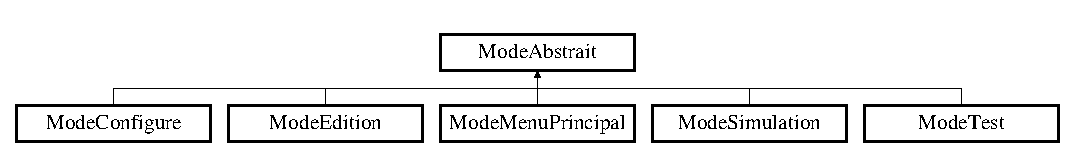
\includegraphics[height=1.671642cm]{class_mode_abstrait}
\end{center}
\end{figure}
\subsection*{Public Member Functions}
\begin{DoxyCompactItemize}
\item 
\hyperlink{group__inf2990_gabad253bb2da30a5c01334977350227bf}{Mode\+Abstrait} ()
\item 
virtual \hyperlink{group__inf2990_ga2756d0b2d692a1bd4c3022a54fc8ce7e}{$\sim$\+Mode\+Abstrait} ()
\item 
virtual void \hyperlink{group__inf2990_ga8e3435fa3ebceb99920d56c72553cd25}{sauvegarder} ()
\item 
virtual void \hyperlink{group__inf2990_ga4a3c7cb5f7c7b04ffd27bbec9c46598d}{charger} ()
\item 
virtual void \hyperlink{group__inf2990_gab8875030f948360faf5107bc14b9eaad}{gerer\+Touche\+Plus} ()
\item 
virtual void \hyperlink{group__inf2990_ga2e6da80aa0fff94c0e86882e34c0243c}{gerer\+Touche\+Moins} ()
\item 
virtual void \hyperlink{group__inf2990_ga117f1c540d2e4fc84cba6c5a8ae24282}{gerer\+Touche\+Echappe} ()
\item 
virtual void \hyperlink{group__inf2990_ga00ffd8fe79674db29904dc220980f9ac}{gerer\+ToucheB} ()
\item 
virtual void \hyperlink{group__inf2990_ga04335a9fa5643227372e5eba3f526d8c}{gerer\+ToucheC} ()
\item 
virtual void \hyperlink{group__inf2990_ga10b4fac21ab4f841821d56777a478605}{gerer\+ToucheD} ()
\item 
virtual void \hyperlink{group__inf2990_gaeb5e4436a3cf8e3b2183ad0fcea47ff0}{gerer\+ToucheE} ()
\item 
virtual void \hyperlink{group__inf2990_gad857df051fef2556d98511b1e187115b}{gerer\+ToucheJ} ()
\item 
virtual void \hyperlink{group__inf2990_gacd85c3fdde471e69c53f48e004eea5c9}{gerer\+ToucheK} ()
\item 
virtual void \hyperlink{group__inf2990_ga7ded1b826180aa17ba44b77e34b1378d}{gerer\+ToucheL} ()
\item 
virtual void \hyperlink{group__inf2990_gab3ffe986a6473abefcb6dd89ee97dad6}{gerer\+ToucheR} ()
\item 
virtual void \hyperlink{group__inf2990_gac2f9d2afbdd6a0884f29294448654109}{gerer\+ToucheS} ()
\item 
virtual void \hyperlink{group__inf2990_ga14779bbf49377203a1be23a6ab9a4e1c}{gerer\+ToucheT} ()
\item 
virtual void \hyperlink{group__inf2990_ga0487016a9f44515dedc5aca95a63521b}{gerer\+ToucheZ} ()
\item 
virtual void \hyperlink{group__inf2990_ga19af4f447726c43f7deffbeda449b37c}{gerer\+Touche\+C\+T\+R\+LavecS} ()
\item 
virtual void \hyperlink{group__inf2990_gaf8b8b6480e870db52c8d7f2eca1c46e3}{gerer\+Touche\+C\+T\+R\+LavecN} ()
\item 
virtual void \hyperlink{group__inf2990_ga8d744898a2fd768b38d54fb5d156b4ce}{gerer\+Touche\+C\+T\+R\+LavecO} ()
\item 
virtual void \hyperlink{group__inf2990_gab6ee3a82d4d72732eaee52bc94ae7788}{gerer\+Touche1} ()
\item 
virtual void \hyperlink{group__inf2990_gaaf53f50c4ee84710c90e6c23a846cb0d}{gerer\+Touche2} ()
\item 
virtual void \hyperlink{group__inf2990_ga051a12b7f5651bc563892fa0a9d8f43b}{gerer\+Touche3} ()
\item 
virtual void \hyperlink{group__inf2990_ga6105f049dc154822017bb351c5155d18}{gerer\+Fleche\+Gauche} ()
\item 
virtual void \hyperlink{group__inf2990_ga55aaba6ce98e1d06716343faf5c5d276}{gerer\+Fleche\+Bas} ()
\item 
virtual void \hyperlink{group__inf2990_ga584774d3533b185fe77cad0c03686ab7}{gerer\+Fleche\+Haut} ()
\item 
virtual void \hyperlink{group__inf2990_ga9a3b727787ee97e8b90ea76295954f2b}{gerer\+Fleche\+Droit} ()
\item 
virtual void \hyperlink{group__inf2990_gae1b7e992530f7b02fdca9a802045eb1c}{gerer\+Barre\+Despacement} ()
\item 
virtual void \hyperlink{group__inf2990_gaa53296cda85d7e3c2f71915a2bbbb5c5}{gerer\+Touche\+Arriere} ()
\item 
virtual void \hyperlink{group__inf2990_gad343a9e6224ea86ba3aed3f10e018b6f}{gerer\+Touche\+Control\+Enfoncee} ()
\item 
virtual void \hyperlink{group__inf2990_ga7c83c75556b4b87d0c1478b10095db4e}{gerer\+Touche\+Control\+Relachee} ()
\item 
virtual void \hyperlink{group__inf2990_ga043a247f2dd09340031b6c8d0f70022d}{gerer\+Touche\+Supprimer} ()
\item 
virtual void \hyperlink{group__inf2990_ga159f4492058ec4567c27aff250fb8bd2}{gerer\+Clic\+Droit\+Enfonce} (const int \&x, const int \&y)
\item 
virtual void \hyperlink{group__inf2990_ga35cccb4de15f88d993df9323b9e0f69b}{gerer\+Clic\+Droit\+Relache} (const int \&x, const int \&y)
\item 
virtual void \hyperlink{group__inf2990_ga9162c07771f10b41c826f24f205e1837}{gerer\+Clic\+Gauche\+Enfonce} (const int \&x, const int \&y)
\item 
virtual void \hyperlink{group__inf2990_ga8759a938db650d28bd01c95406857bf0}{gerer\+Clic\+Gauche\+Relache} (const int \&x, const int \&y)
\item 
virtual void \hyperlink{group__inf2990_gaa7d8f602067ce5521dbe81a495432d03}{gerer\+Mouvement\+Souris} (const int \&x, const int \&y)
\item 
virtual void \hyperlink{group__inf2990_ga641affa53d236daeaae109d472b32f92}{gerer\+Molette\+Souris} (const int \&delta)
\item 
int \hyperlink{group__inf2990_ga729cb1e21af5c283e252647a7a413a21}{obtenir\+Type\+Mode} ()
\end{DoxyCompactItemize}
\subsection*{Protected Attributes}
\begin{DoxyCompactItemize}
\item 
int {\bfseries type\+Mode\+\_\+}\hypertarget{class_mode_abstrait_a8abb87b9dbe104a45069c6e9e84f7db3}{}\label{class_mode_abstrait_a8abb87b9dbe104a45069c6e9e84f7db3}

\end{DoxyCompactItemize}


\subsection{Detailed Description}
Classe qui repr�sente le mode abstrait de notre machine � modes. 

Cette classe s\textquotesingle{}occupe de d�clarer les fonctions qui seront impl�ment�s dans les �tats d�riv�s. \begin{DoxyAuthor}{Author}
Simon-\/\+Pierre Desjardins 
\end{DoxyAuthor}
\begin{DoxyDate}{Date}
2016-\/02-\/14 
\end{DoxyDate}


The documentation for this class was generated from the following files\+:\begin{DoxyCompactItemize}
\item 
Sources/\+D\+L\+L/\+Machine\+A\+Modes/\hyperlink{_mode_abstrait_8h}{Mode\+Abstrait.\+h}\item 
Sources/\+D\+L\+L/\+Machine\+A\+Modes/\hyperlink{_mode_abstrait_8cpp}{Mode\+Abstrait.\+cpp}\end{DoxyCompactItemize}

\hypertarget{class_mode_configure}{}\section{Mode\+Configure Class Reference}
\label{class_mode_configure}\index{Mode\+Configure@{Mode\+Configure}}


Classe qui repr�sente le mode configure de notre machine � modes.  




{\ttfamily \#include $<$Mode\+Configure.\+h$>$}

Inheritance diagram for Mode\+Configure\+:\begin{figure}[H]
\begin{center}
\leavevmode
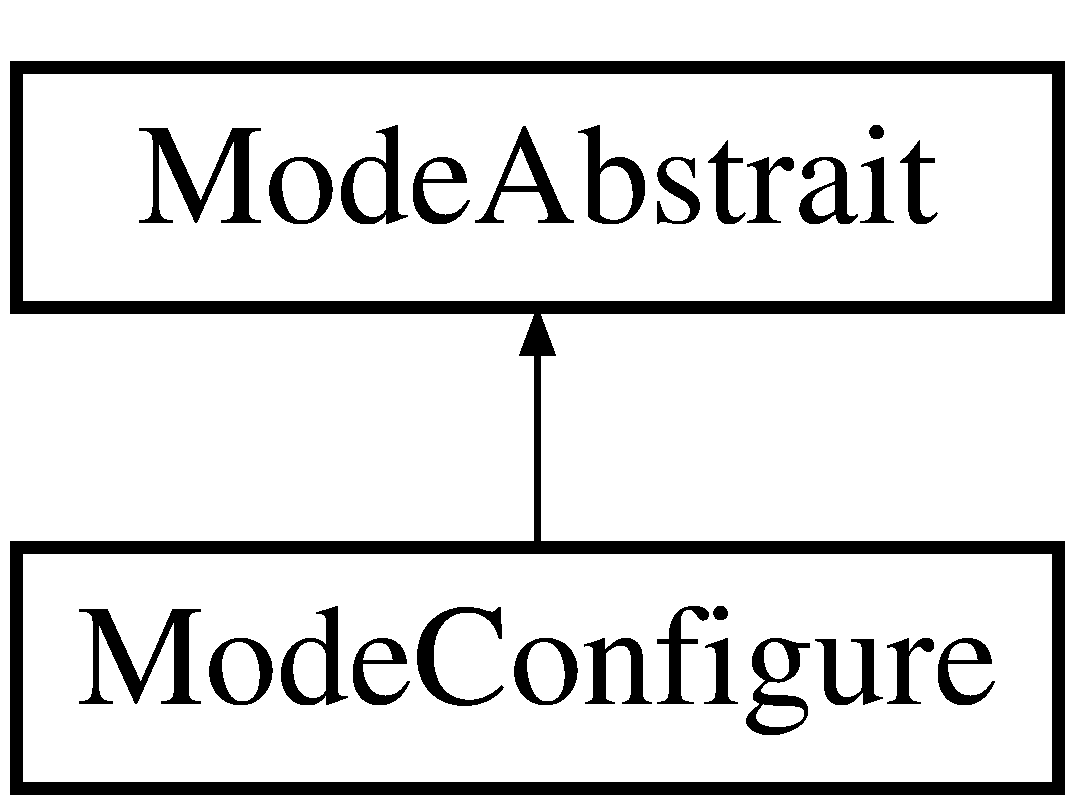
\includegraphics[height=2.000000cm]{class_mode_configure}
\end{center}
\end{figure}
\subsection*{Public Member Functions}
\begin{DoxyCompactItemize}
\item 
\hyperlink{group__inf2990_gabbf5cdcec1e0b0d4639f606684bb0a40}{Mode\+Configure} ()
\item 
virtual \hyperlink{group__inf2990_gab39845bb67a2c8c4ed42c996d826052a}{$\sim$\+Mode\+Configure} ()
\end{DoxyCompactItemize}
\subsection*{Additional Inherited Members}


\subsection{Detailed Description}
Classe qui repr�sente le mode configure de notre machine � modes. 

Cette classe s\textquotesingle{}occupe d\textquotesingle{}impl�menter les fonctions du mode configure

\begin{DoxyAuthor}{Author}
Simon-\/\+Pierre Desjardins 
\end{DoxyAuthor}
\begin{DoxyDate}{Date}
2016-\/02-\/14 
\end{DoxyDate}


The documentation for this class was generated from the following files\+:\begin{DoxyCompactItemize}
\item 
Sources/\+D\+L\+L/\+Machine\+A\+Modes/\hyperlink{_mode_configure_8h}{Mode\+Configure.\+h}\item 
Sources/\+D\+L\+L/\+Machine\+A\+Modes/\hyperlink{_mode_configure_8cpp}{Mode\+Configure.\+cpp}\end{DoxyCompactItemize}

\hypertarget{class_mode_edition}{}\section{Mode\+Edition Class Reference}
\label{class_mode_edition}\index{Mode\+Edition@{Mode\+Edition}}


Classe qui repr�sente le mode edition de notre machine � modes.  




{\ttfamily \#include $<$Mode\+Edition.\+h$>$}

Inheritance diagram for Mode\+Edition\+:\begin{figure}[H]
\begin{center}
\leavevmode
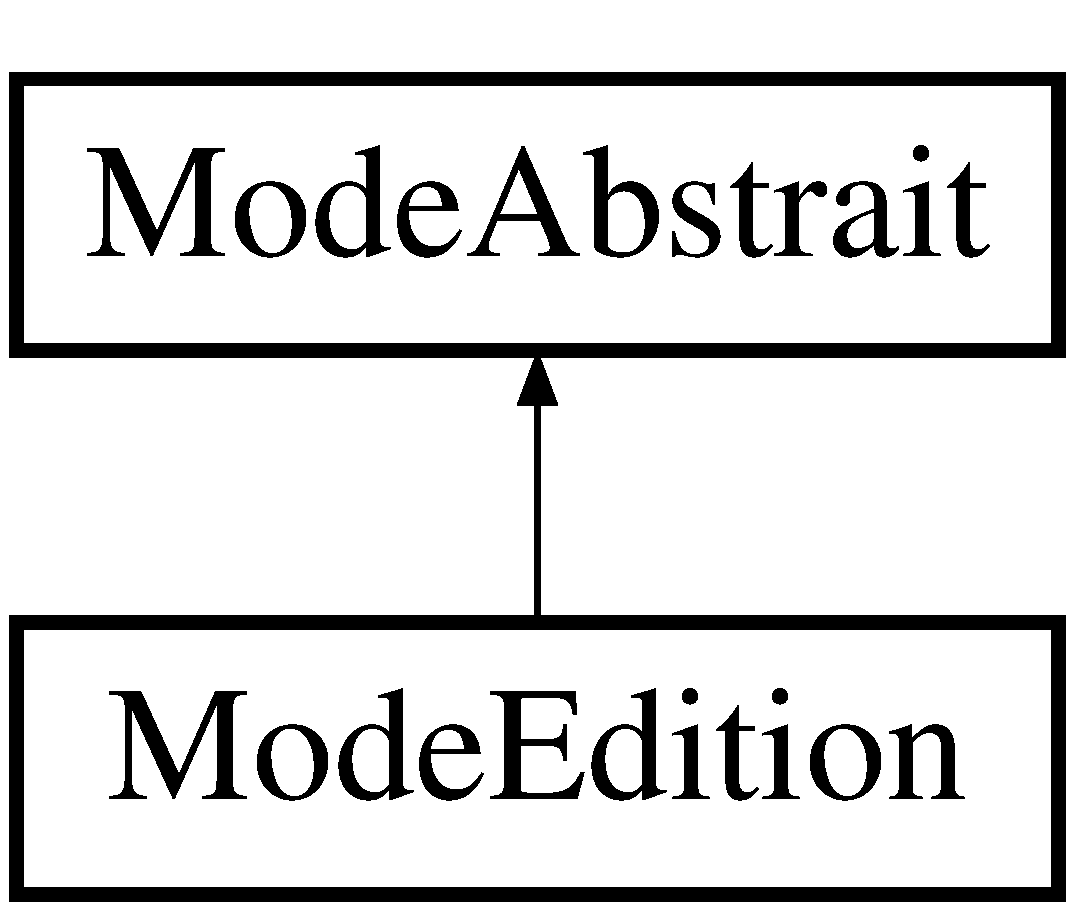
\includegraphics[height=2.000000cm]{class_mode_edition}
\end{center}
\end{figure}
\subsection*{Public Member Functions}
\begin{DoxyCompactItemize}
\item 
\hyperlink{group__inf2990_ga268c053a2916d15b9b786d32178de102}{Mode\+Edition} ()
\item 
virtual \hyperlink{group__inf2990_gae3468af0e1eea13d063a084401c34a05}{$\sim$\+Mode\+Edition} ()
\item 
virtual void \hyperlink{group__inf2990_ga94151a179e28165043604700379c4b84}{gerer\+Touche\+Plus} ()
\item 
virtual void \hyperlink{group__inf2990_gac0c1355eb798570bf72f623758e5e902}{gerer\+Touche\+Moins} ()
\item 
virtual void \hyperlink{group__inf2990_gac39246bc68c969257a222055ecb05d8f}{gerer\+Touche\+Echappe} ()
\item 
virtual void \hyperlink{group__inf2990_ga83f56849596c18ef90973f003167387b}{gerer\+ToucheC} ()
\item 
virtual void \hyperlink{group__inf2990_gab96daf92f058e3e17ca4e05d042255fd}{gerer\+ToucheD} ()
\item 
virtual void \hyperlink{group__inf2990_gaf7f67f0346f3b4b9232e32b2921b8858}{gerer\+ToucheE} ()
\item 
virtual void \hyperlink{group__inf2990_gadb0c721d1e46be5c937de5ac9f2d2dd0}{gerer\+ToucheR} ()
\item 
virtual void \hyperlink{group__inf2990_gab0551432df7752b9dbfdaf31b9f4c0e2}{gerer\+ToucheS} ()
\item 
virtual void \hyperlink{group__inf2990_ga7b37a9c3df9362d84d9e5d5a87261e1c}{gerer\+ToucheT} ()
\item 
virtual void \hyperlink{group__inf2990_ga5ddfbdf09b476985c9a7dec86402322d}{gerer\+ToucheZ} ()
\item 
virtual void \hyperlink{group__inf2990_gaa39347b336958ada753dcd8eacc0a4fd}{gerer\+Touche\+C\+T\+R\+LavecS} ()
\item 
virtual void \hyperlink{group__inf2990_ga3645c71a7ba328892020eccae334d8b8}{gerer\+Touche\+C\+T\+R\+LavecN} ()
\item 
virtual void \hyperlink{group__inf2990_gab78b5d728912c2f05b6bb438906a335b}{gerer\+Touche\+C\+T\+R\+LavecO} ()
\item 
virtual void \hyperlink{group__inf2990_ga49ed034a0dc18b1f5e003c3720a781e8}{gerer\+Touche1} ()
\item 
virtual void \hyperlink{group__inf2990_ga5c78880c6893dd2b08411dab0efce427}{gerer\+Touche2} ()
\item 
virtual void \hyperlink{group__inf2990_ga58287cda8cda127bc9dac8587101130a}{gerer\+Fleche\+Gauche} ()
\item 
virtual void \hyperlink{group__inf2990_ga7fb472a3830195719024b2be32078d38}{gerer\+Fleche\+Bas} ()
\item 
virtual void \hyperlink{group__inf2990_gaeaa66ffadc44aebc5133151d47e6c89c}{gerer\+Fleche\+Haut} ()
\item 
virtual void \hyperlink{group__inf2990_ga29fc411065f2455a5f5d957519658dd8}{gerer\+Fleche\+Droit} ()
\item 
virtual void \hyperlink{group__inf2990_ga5d20e0d87f8612bf221ef4e04a01d032}{gerer\+Touche\+Control\+Enfoncee} ()
\item 
virtual void \hyperlink{group__inf2990_gaa077418f30d52be402fa5a4343805cbf}{gerer\+Touche\+Control\+Relachee} ()
\item 
virtual void \hyperlink{group__inf2990_ga47fcfe249f809739b16a4b77d5d0a51b}{gerer\+Touche\+Alt\+Enfoncee} ()
\item 
virtual void \hyperlink{group__inf2990_ga3f72484a942b226c7a3abfe1bf1e47c7}{gerer\+Touche\+Alt\+Relachee} ()
\item 
virtual void \hyperlink{group__inf2990_gaa9c3d2d3afdb3918f855e9b826bac4e5}{gerer\+Clic\+Droit\+Enfonce} (const int \&x, const int \&y)
\item 
virtual void \hyperlink{group__inf2990_gaabdb85a8e87a58c4d8f5af92702c6b67}{gerer\+Clic\+Droit\+Relache} (const int \&x, const int \&y)
\item 
virtual void \hyperlink{group__inf2990_ga5cec4050215dc46982f6b85a763dd6aa}{gerer\+Clic\+Gauche\+Enfonce} (const int \&x, const int \&y)
\item 
virtual void \hyperlink{group__inf2990_gafd316b4efa2e5aa77d9f834797d1b168}{gerer\+Clic\+Gauche\+Relache} (const int \&x, const int \&y)
\item 
virtual void \hyperlink{group__inf2990_gaea2093aede7e9ff847ffbff7f239e676}{gerer\+Mouvement\+Souris} (const int \&x, const int \&y)
\item 
virtual void \hyperlink{group__inf2990_ga4564a7cafcfb91e2737e9be2d507cd37}{gerer\+Molette\+Souris} (const int \&delta)
\item 
virtual void \hyperlink{group__inf2990_ga1f2627982c6c534705c3f7a1b08a8517}{gerer\+Touche\+Supprimer} ()
\item 
virtual void \hyperlink{group__inf2990_ga2d41ac8efcf339dba4b5d1426d3400b7}{sauvegarder} ()
\item 
virtual void \hyperlink{group__inf2990_ga9af77303c3e86a19f1fe004e79fcfc32}{charger} ()
\end{DoxyCompactItemize}
\subsection*{Protected Attributes}
\begin{DoxyCompactItemize}
\item 
std\+::unique\+\_\+ptr$<$ \hyperlink{class_visiteur_suppression}{Visiteur\+Suppression} $>$ {\bfseries visiteur\+Suppression\+\_\+}\hypertarget{class_mode_edition_afb2edadce01658138d72c8f6d64cb43d}{}\label{class_mode_edition_afb2edadce01658138d72c8f6d64cb43d}

\item 
int {\bfseries ancien\+Souris\+X\+\_\+} \{ 0 \}\hypertarget{class_mode_edition_a374bbb7ad5b5e75b7d4bb66c8727de02}{}\label{class_mode_edition_a374bbb7ad5b5e75b7d4bb66c8727de02}

\item 
int {\bfseries ancien\+Souris\+Y\+\_\+} \{ 0 \}\hypertarget{class_mode_edition_af3ce579a746b7cf363f0a508377609e1}{}\label{class_mode_edition_af3ce579a746b7cf363f0a508377609e1}

\end{DoxyCompactItemize}


\subsection{Detailed Description}
Classe qui repr�sente le mode edition de notre machine � modes. 

\begin{DoxyAuthor}{Author}
Simon-\/\+Pierre Desjardins 
\end{DoxyAuthor}
\begin{DoxyDate}{Date}
2016-\/02-\/14
\end{DoxyDate}
Cette classe s\textquotesingle{}occupe d\textquotesingle{}impl�menter les fonctions du mode edition 

The documentation for this class was generated from the following files\+:\begin{DoxyCompactItemize}
\item 
Sources/\+D\+L\+L/\+Machine\+A\+Modes/\hyperlink{_mode_edition_8h}{Mode\+Edition.\+h}\item 
Sources/\+D\+L\+L/\+Machine\+A\+Modes/\hyperlink{_mode_edition_8cpp}{Mode\+Edition.\+cpp}\end{DoxyCompactItemize}

\hypertarget{class_mode_menu_principal}{}\section{Mode\+Menu\+Principal Class Reference}
\label{class_mode_menu_principal}\index{Mode\+Menu\+Principal@{Mode\+Menu\+Principal}}


Classe qui repr�sente le mode menu principal de notre machine � modes.  




{\ttfamily \#include $<$Mode\+Menu\+Principal.\+h$>$}

Inheritance diagram for Mode\+Menu\+Principal\+:\begin{figure}[H]
\begin{center}
\leavevmode
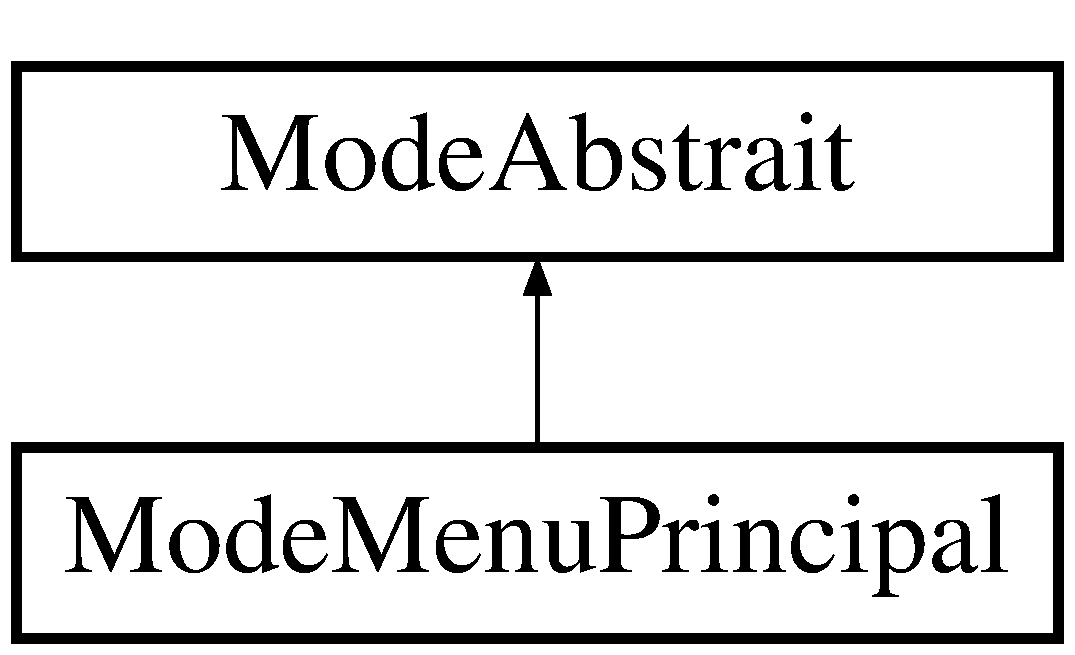
\includegraphics[height=2.000000cm]{class_mode_menu_principal}
\end{center}
\end{figure}
\subsection*{Public Member Functions}
\begin{DoxyCompactItemize}
\item 
\hyperlink{group__inf2990_gafe4d63e2701449fc1acfa16da10cab3e}{Mode\+Menu\+Principal} ()
\item 
virtual \hyperlink{group__inf2990_ga7ac40f3869bdbf8714200623af012fd9}{$\sim$\+Mode\+Menu\+Principal} ()
\end{DoxyCompactItemize}
\subsection*{Additional Inherited Members}


\subsection{Detailed Description}
Classe qui repr�sente le mode menu principal de notre machine � modes. 

Cette classe s\textquotesingle{}occupe d\textquotesingle{}impl�menter les fonctions du mode menu principal

\begin{DoxyAuthor}{Author}
Simon-\/\+Pierre Desjardins 
\end{DoxyAuthor}
\begin{DoxyDate}{Date}
2016-\/02-\/14 
\end{DoxyDate}


The documentation for this class was generated from the following files\+:\begin{DoxyCompactItemize}
\item 
Sources/\+D\+L\+L/\+Machine\+A\+Modes/\hyperlink{_mode_menu_principal_8h}{Mode\+Menu\+Principal.\+h}\item 
Sources/\+D\+L\+L/\+Machine\+A\+Modes/\hyperlink{_mode_menu_principal_8cpp}{Mode\+Menu\+Principal.\+cpp}\end{DoxyCompactItemize}

\hypertarget{class_mode_simulation}{}\section{Mode\+Simulation Class Reference}
\label{class_mode_simulation}\index{Mode\+Simulation@{Mode\+Simulation}}


Classe qui repr�sente le mode simulation de notre machine � modes.  




{\ttfamily \#include $<$Mode\+Simulation.\+h$>$}

Inheritance diagram for Mode\+Simulation\+:\begin{figure}[H]
\begin{center}
\leavevmode
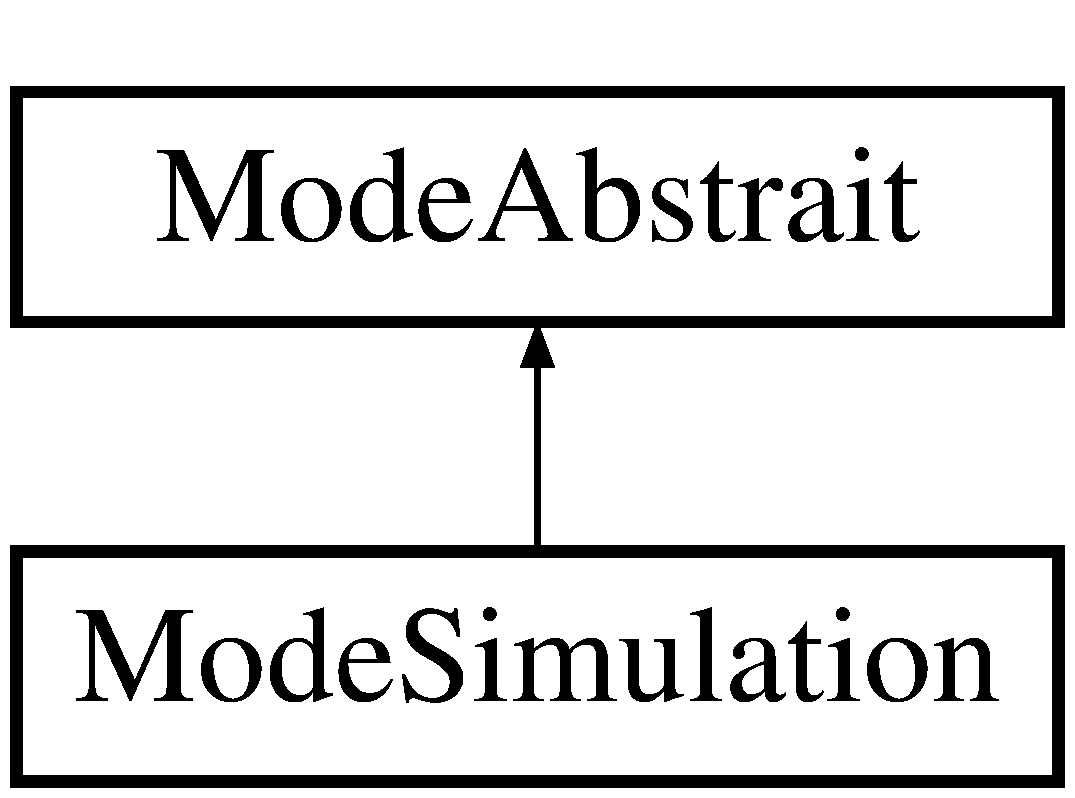
\includegraphics[height=2.000000cm]{class_mode_simulation}
\end{center}
\end{figure}
\subsection*{Public Member Functions}
\begin{DoxyCompactItemize}
\item 
\hyperlink{group__inf2990_ga9f9172ddaa09010a6f0c2a3abe94c96e}{Mode\+Simulation} ()
\item 
virtual \hyperlink{group__inf2990_ga92208c0b9cdb59bd0c95f78f91b5c515}{$\sim$\+Mode\+Simulation} ()
\end{DoxyCompactItemize}
\subsection*{Additional Inherited Members}


\subsection{Detailed Description}
Classe qui repr�sente le mode simulation de notre machine � modes. 

Cette classe s\textquotesingle{}occupe d\textquotesingle{}impl�menter les fonctions du mode simulation

\begin{DoxyAuthor}{Author}
Simon-\/\+Pierre Desjardins 
\end{DoxyAuthor}
\begin{DoxyDate}{Date}
2016-\/02-\/14 
\end{DoxyDate}


The documentation for this class was generated from the following files\+:\begin{DoxyCompactItemize}
\item 
Sources/\+D\+L\+L/\+Machine\+A\+Modes/\hyperlink{_mode_simulation_8h}{Mode\+Simulation.\+h}\item 
Sources/\+D\+L\+L/\+Machine\+A\+Modes/\hyperlink{_mode_simulation_8cpp}{Mode\+Simulation.\+cpp}\end{DoxyCompactItemize}

\hypertarget{class_mode_test}{}\section{Mode\+Test Class Reference}
\label{class_mode_test}\index{Mode\+Test@{Mode\+Test}}


Classe qui repr�sente le mode test de notre machine � modes.  




{\ttfamily \#include $<$Mode\+Test.\+h$>$}

Inheritance diagram for Mode\+Test\+:\begin{figure}[H]
\begin{center}
\leavevmode
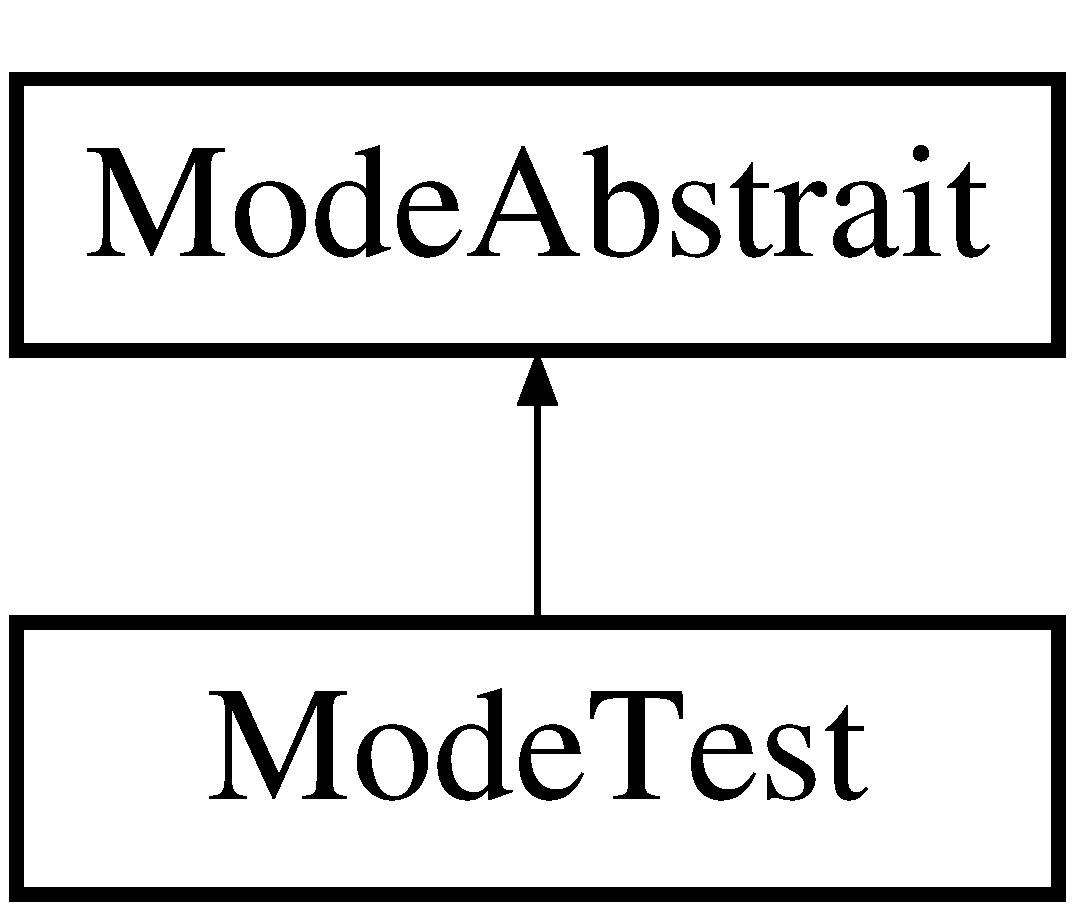
\includegraphics[height=2.000000cm]{class_mode_test}
\end{center}
\end{figure}
\subsection*{Public Member Functions}
\begin{DoxyCompactItemize}
\item 
\hyperlink{group__inf2990_ga8835d51c0957eb6d104e112309bf44f9}{Mode\+Test} ()
\item 
virtual \hyperlink{group__inf2990_ga11f99d8a7a9a8bb928506ed416f6f280}{$\sim$\+Mode\+Test} ()
\end{DoxyCompactItemize}
\subsection*{Additional Inherited Members}


\subsection{Detailed Description}
Classe qui repr�sente le mode test de notre machine � modes. 

Cette classe s\textquotesingle{}occupe d\textquotesingle{}impl�menter les fonctions du mode test

\begin{DoxyAuthor}{Author}
Simon-\/\+Pierre Desjardins 
\end{DoxyAuthor}
\begin{DoxyDate}{Date}
2016-\/02-\/14 
\end{DoxyDate}


The documentation for this class was generated from the following files\+:\begin{DoxyCompactItemize}
\item 
Sources/\+D\+L\+L/\+Machine\+A\+Modes/\hyperlink{_mode_test_8h}{Mode\+Test.\+h}\item 
Sources/\+D\+L\+L/\+Machine\+A\+Modes/\hyperlink{_mode_test_8cpp}{Mode\+Test.\+cpp}\end{DoxyCompactItemize}

\hypertarget{class_noeud_abstrait}{}\section{Noeud\+Abstrait Class Reference}
\label{class_noeud_abstrait}\index{Noeud\+Abstrait@{Noeud\+Abstrait}}


Classe de base du patron composite utilis�e pour cr�er l\textquotesingle{}arbre de rendu.  




{\ttfamily \#include $<$Noeud\+Abstrait.\+h$>$}

Inheritance diagram for Noeud\+Abstrait\+:\begin{figure}[H]
\begin{center}
\leavevmode
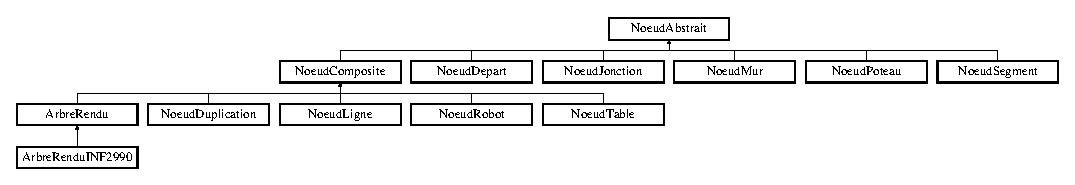
\includegraphics[height=2.043796cm]{class_noeud_abstrait}
\end{center}
\end{figure}
\subsection*{Public Member Functions}
\begin{DoxyCompactItemize}
\item 
\hyperlink{group__inf2990_ga1d1340ee36824e0c6013e65a1306d8f3}{Noeud\+Abstrait} (const std\+::string \&type=std\+::string\{\char`\"{}\char`\"{}\})
\begin{DoxyCompactList}\small\item\em Constructeur. \end{DoxyCompactList}\item 
virtual \hyperlink{group__inf2990_ga0ab3f7ab838e8349113da5074abcdc3a}{$\sim$\+Noeud\+Abstrait} ()
\begin{DoxyCompactList}\small\item\em Destructeur. \end{DoxyCompactList}\item 
\hyperlink{class_noeud_abstrait}{Noeud\+Abstrait} $\ast$ \hyperlink{group__inf2990_gaa2ac8c4cd02d88c312b92c65e07ed6d9}{obtenir\+Parent} ()
\begin{DoxyCompactList}\small\item\em Obtient le parent de ce noeud. \end{DoxyCompactList}\item 
const \hyperlink{class_noeud_abstrait}{Noeud\+Abstrait} $\ast$ \hyperlink{group__inf2990_gaf063d208bc4764b1fd2c4e76ec0469b9}{obtenir\+Parent} () const 
\begin{DoxyCompactList}\small\item\em Obtient le parent de ce noeud (version constante). \end{DoxyCompactList}\item 
void \hyperlink{group__inf2990_ga7787ab59ecc1e6119287459a7154f307}{assigner\+Parent} (\hyperlink{class_noeud_abstrait}{Noeud\+Abstrait} $\ast$parent)
\begin{DoxyCompactList}\small\item\em Assigne le parent de ce noeud. \end{DoxyCompactList}\item 
const glm\+::dvec3 \& \hyperlink{group__inf2990_ga62d73f67c3b33e2cb106630bd1736a58}{obtenir\+Position\+Relative} () const 
\begin{DoxyCompactList}\small\item\em Obtient la position relative du noeud. \end{DoxyCompactList}\item 
void \hyperlink{group__inf2990_ga11e12e42b05a5327c92cd7fd1b7e5a24}{assigner\+Position\+Relative} (const glm\+::dvec3 \&position\+Relative)
\begin{DoxyCompactList}\small\item\em Assigne la position relative du noeud. \end{DoxyCompactList}\item 
double \hyperlink{group__inf2990_gadde64226b78ccb9bd801ff7b04ee5545}{obtenir\+Angle\+Rotation} () const 
\begin{DoxyCompactList}\small\item\em Obtient l\textquotesingle{}angle de rotation du noeud. \end{DoxyCompactList}\item 
void \hyperlink{group__inf2990_ga356d70c0535b1a9aed118d1f5139d953}{assigner\+Angle\+Rotation} (const double \&angle\+Rotation)
\begin{DoxyCompactList}\small\item\em Assigne l\textquotesingle{}angle de rotation du noeud par rapport au plan xy. \end{DoxyCompactList}\item 
double \hyperlink{group__inf2990_gaa2ef40d71626411739cc9ab6343c9ce2}{obtenir\+Facteur\+Mise\+A\+Echelle} () const 
\begin{DoxyCompactList}\small\item\em Obtient le facteur de dimension du noeud. \end{DoxyCompactList}\item 
void \hyperlink{group__inf2990_ga47d44227a5e154a2548121477ad266b3}{assigner\+Facteur\+Mise\+A\+Echelle} (const double \&facteur\+Dimension)
\begin{DoxyCompactList}\small\item\em Assigne le facteur de dimension. \end{DoxyCompactList}\item 
utilitaire\+::\+Quad\+Englobant \hyperlink{group__inf2990_gaa40880839d94bd0032e31689aa368b61}{obtenir\+Quad\+Englobant\+Courant} () const 
\begin{DoxyCompactList}\small\item\em Obtient le quadrilat�re englobant du noeud. \end{DoxyCompactList}\item 
void \hyperlink{group__inf2990_ga11b542cc1a969669a2a30375add3f840}{assigner\+Quad\+Englobant\+Courant} (const utilitaire\+::\+Quad\+Englobant \&quad)
\begin{DoxyCompactList}\small\item\em Assigne le quadrilat�re englobant du noeud. \end{DoxyCompactList}\item 
utilitaire\+::\+Quad\+Englobant \hyperlink{group__inf2990_ga6d28c0d37a18b37c85a5096dea955fb2}{obtenir\+Quad\+Englobant\+Modele} () const 
\begin{DoxyCompactList}\small\item\em Obtenir la boite englobante du mod�le. \end{DoxyCompactList}\item 
const std\+::string \& \hyperlink{group__inf2990_ga2df7c53ab456cc88bce73f7eb913e3e6}{obtenir\+Type} () const 
\begin{DoxyCompactList}\small\item\em Obtient le type du noeud. \end{DoxyCompactList}\item 
void \hyperlink{group__inf2990_gad5205d1e1b63fb66175a8580261d5eea}{assigner\+Affiche} (bool affiche)
\begin{DoxyCompactList}\small\item\em �crit l\textquotesingle{}�tat de l\textquotesingle{}affichage du du noeud. \end{DoxyCompactList}\item 
bool \hyperlink{group__inf2990_ga07fc02e86d59ccd2680f9e5f5b8e373d}{est\+Affiche} () const 
\begin{DoxyCompactList}\small\item\em V�rifie si le noeud se fait afficher. \end{DoxyCompactList}\item 
void \hyperlink{group__inf2990_ga0f39647390d357d8662a870f0c76242c}{assigner\+Selection} (bool selectionne)
\begin{DoxyCompactList}\small\item\em �crit l\textquotesingle{}�tat de la s�lection du noeud. \end{DoxyCompactList}\item 
bool \hyperlink{group__inf2990_ga8fb7a3313ce4d361ef7ec8e45ba8add5}{est\+Selectionne} () const 
\begin{DoxyCompactList}\small\item\em V�rifie si le noeud est s�lectionn�. \end{DoxyCompactList}\item 
void \hyperlink{group__inf2990_ga397add0bac7ec3b842598a2085990b7d}{assigner\+Est\+Selectionnable} (bool selectionnable)
\begin{DoxyCompactList}\small\item\em �crit si le noeud peut �tre s�lectionn� ou non. \end{DoxyCompactList}\item 
bool \hyperlink{group__inf2990_gaa3f3a34571af62de0da5db2d8f54f690}{est\+Selectionnable} () const 
\begin{DoxyCompactList}\small\item\em V�rifie si le noeud est s�lectionnable. \end{DoxyCompactList}\item 
void \hyperlink{group__inf2990_gabb7f3756a4094dc588690126ec0703d3}{assigner\+Est\+Enregistrable} (bool enregistrable)
\begin{DoxyCompactList}\small\item\em �crit si le noeud peut �tre enregistr� ou non. \end{DoxyCompactList}\item 
bool \hyperlink{group__inf2990_ga6a6af3639f1b4e3e33a126703376dcec}{est\+Enregistrable} () const 
\begin{DoxyCompactList}\small\item\em V�rifie si le noeud est enregistrable. \end{DoxyCompactList}\item 
bool \hyperlink{group__inf2990_ga5b13edb47520befa3e17eb3097506791}{assigner\+Est\+Duplicable} (bool \hyperlink{group__inf2990_ga4122c4ce180a62e68edb8e55b54c30f1}{est\+Duplicable})
\begin{DoxyCompactList}\small\item\em �crit si le noeud peut �tre enregistr� ou non. \end{DoxyCompactList}\item 
bool \hyperlink{group__inf2990_ga4122c4ce180a62e68edb8e55b54c30f1}{est\+Duplicable} () const 
\begin{DoxyCompactList}\small\item\em V�rifie si l\textquotesingle{}objet peut �tre dupliqu�. \end{DoxyCompactList}\item 
void \hyperlink{group__inf2990_ga1f533acce98fbad7fa82758ccaea55ff}{assigner\+Objet\+Rendu} (modele\+::\+Modele3D const $\ast$modele, opengl\+::\+V\+BO const $\ast$liste)
\begin{DoxyCompactList}\small\item\em Assigne le mod�le3D et la liste d\textquotesingle{}affichage du noeud courant. \end{DoxyCompactList}\item 
virtual unsigned int \hyperlink{group__inf2990_gad854800087fd6c13f1a63589caefb41d}{calculer\+Profondeur} () const 
\begin{DoxyCompactList}\small\item\em Calcule la profondeur de l\textquotesingle{}arbre sous le noeud courant. \end{DoxyCompactList}\item 
virtual void \hyperlink{group__inf2990_ga55435ee83860c6a2101334ba67bbd9b6}{vider} ()
\begin{DoxyCompactList}\small\item\em Vide le noeud de ses enfants. \end{DoxyCompactList}\item 
virtual void \hyperlink{group__inf2990_ga2ab3dc520026d1ad77aa848981688bfd}{effacer} (const \hyperlink{class_noeud_abstrait}{Noeud\+Abstrait} $\ast$noeud)
\begin{DoxyCompactList}\small\item\em Efface le noeud pass� en param�tre. \end{DoxyCompactList}\item 
virtual const \hyperlink{class_noeud_abstrait}{Noeud\+Abstrait} $\ast$ \hyperlink{group__inf2990_gaeda0df98faf404765d985fcde60fb924}{chercher} (const std\+::string \&type\+Noeud) const 
\begin{DoxyCompactList}\small\item\em Cherche un noeud par le type (sur un noeud constant). \end{DoxyCompactList}\item 
virtual \hyperlink{class_noeud_abstrait}{Noeud\+Abstrait} $\ast$ \hyperlink{group__inf2990_ga0868ae108165b071f6c8a68a7265c770}{chercher} (const std\+::string \&type\+Noeud)
\begin{DoxyCompactList}\small\item\em Cherche un noeud par le type. \end{DoxyCompactList}\item 
virtual const \hyperlink{class_noeud_abstrait}{Noeud\+Abstrait} $\ast$ \hyperlink{group__inf2990_gac334b078c318e39a065b85572778bf13}{chercher} (unsigned int indice) const 
\begin{DoxyCompactList}\small\item\em Cherche un noeud enfant selon l\textquotesingle{}indice (sur un noeud constant). \end{DoxyCompactList}\item 
virtual \hyperlink{class_noeud_abstrait}{Noeud\+Abstrait} $\ast$ \hyperlink{group__inf2990_ga13f7e9a637f7439b1a0cec0c49f6fa88}{chercher} (unsigned int indice)
\begin{DoxyCompactList}\small\item\em Cherche un noeud enfant selon l\textquotesingle{}indice. \end{DoxyCompactList}\item 
virtual bool \hyperlink{group__inf2990_ga5a6f29be9794a5db96e112727b63d131}{ajouter} (std\+::shared\+\_\+ptr$<$ \hyperlink{class_noeud_abstrait}{Noeud\+Abstrait} $>$ enfant)
\begin{DoxyCompactList}\small\item\em Ajoute un noeud enfant. \end{DoxyCompactList}\item 
virtual unsigned int \hyperlink{group__inf2990_gad5a99959e905fc2d9f0fef16a02546a2}{obtenir\+Nombre\+Enfants} () const 
\begin{DoxyCompactList}\small\item\em Obtient le nombre d\textquotesingle{}enfants du noeud. \end{DoxyCompactList}\item 
virtual void \hyperlink{group__inf2990_ga2516eef94f98d4951baff6fd45020725}{inverser\+Selection} ()
\begin{DoxyCompactList}\small\item\em Changer la s�lection du noeud. \end{DoxyCompactList}\item 
virtual void \hyperlink{group__inf2990_gaf6440c1b4ab6861f0ace6ba410c1fc84}{effacer\+Selection} ()
\begin{DoxyCompactList}\small\item\em Efface les enfants s�lectionn�s. \end{DoxyCompactList}\item 
virtual void \hyperlink{group__inf2990_gaa9b1fa06dad2695ea6870411c62652b3}{selectionner\+Tout} ()
\begin{DoxyCompactList}\small\item\em S�lectionne tous les enfants de m�me que le noeud. \end{DoxyCompactList}\item 
virtual void \hyperlink{group__inf2990_ga4f942bd122fc3402537ecac737c5248a}{deselectionner\+Tout} ()
\begin{DoxyCompactList}\small\item\em D�s�lectionne tous les enfants de m�me que le noeud. \end{DoxyCompactList}\item 
virtual bool \hyperlink{group__inf2990_gae7c702b865babd20ddd30dd776adc82b}{selection\+Existe} () const 
\begin{DoxyCompactList}\small\item\em V�rifier si le noeud ou un de ses enfants est s�lectionn�. \end{DoxyCompactList}\item 
virtual void \hyperlink{group__inf2990_ga13a97383c2081b405fc2e0d97cff80df}{changer\+Mode\+Polygones} (bool est\+Force)
\begin{DoxyCompactList}\small\item\em Change le mode d\textquotesingle{}affichage des polygones. \end{DoxyCompactList}\item 
virtual void \hyperlink{group__inf2990_ga726d9d0a524939f405aeeac3fbd06666}{assigner\+Mode\+Polygones} (G\+Lenum mode\+Polygones)
\begin{DoxyCompactList}\small\item\em Assigne le mode d\textquotesingle{}affichage des polygones. \end{DoxyCompactList}\item 
virtual void \hyperlink{group__inf2990_gae789271ea41032d717b8e4300be05de0}{afficher} () const 
\begin{DoxyCompactList}\small\item\em Affiche le noeud. \end{DoxyCompactList}\item 
virtual void \hyperlink{group__inf2990_ga330df455c8b08440d3c8e64d0a480391}{afficher\+Concret} () const 
\begin{DoxyCompactList}\small\item\em Affiche le noeud de mani�re concr�te. \end{DoxyCompactList}\item 
virtual void \hyperlink{group__inf2990_gadc6ebe69894dbb682fdd0ecb1b6c11e9}{animer} (float dt)
\begin{DoxyCompactList}\small\item\em Anime le noeud. \end{DoxyCompactList}\item 
virtual void \hyperlink{class_noeud_abstrait_a06a1465d51e83f31847bb9b19ec14f66}{accepter\+Visiteur} (\hyperlink{class_visiteur_abstrait}{Visiteur\+Abstrait} $\ast$visiteur)=0\hypertarget{class_noeud_abstrait_a06a1465d51e83f31847bb9b19ec14f66}{}\label{class_noeud_abstrait_a06a1465d51e83f31847bb9b19ec14f66}

\begin{DoxyCompactList}\small\item\em Accepter un visiteur. \end{DoxyCompactList}\item 
virtual modele\+::\+Modele3D const $\ast$ \hyperlink{group__inf2990_ga076097137f68af7d3f86cb459c90b5aa}{get\+Modele} ()
\begin{DoxyCompactList}\small\item\em Retourne le mod�le. \end{DoxyCompactList}\item 
virtual bool {\bfseries obtenir\+En\+Creation} ()\hypertarget{class_noeud_abstrait_aa128f68e207a1a6532fc40eb99f5e24e}{}\label{class_noeud_abstrait_aa128f68e207a1a6532fc40eb99f5e24e}

\item 
virtual void {\bfseries assigner\+En\+Creation} (bool en\+Creation)\hypertarget{class_noeud_abstrait_a4cf779296662a654d8617863332c4f4d}{}\label{class_noeud_abstrait_a4cf779296662a654d8617863332c4f4d}

\item 
void \hyperlink{group__inf2990_gaff4f70778d8f22370ca7ea7cf7d9cd0c}{to\+Json} (rapidjson\+::\+Writer$<$ rapidjson\+::\+File\+Write\+Stream $>$ \&writer)
\begin{DoxyCompactList}\small\item\em convertit un noeud en J\+S\+ON \end{DoxyCompactList}\item 
void \hyperlink{group__inf2990_ga92953ceac94de8b9d33d5b5132d2c269}{from\+Json} (rapidjson\+::\+Value\+::\+Const\+Value\+Iterator noeud\+J\+S\+ON)
\begin{DoxyCompactList}\small\item\em assigne les attributs d\textquotesingle{}un noeud � partir d\textquotesingle{}un J\+S\+ON \end{DoxyCompactList}\end{DoxyCompactItemize}
\subsection*{Protected Attributes}
\begin{DoxyCompactItemize}
\item 
bool \hyperlink{class_noeud_abstrait_a994dc03cfc1a7eb167a5aeaf95ebb87f}{en\+Creation\+\_\+} \{ false \}\hypertarget{class_noeud_abstrait_a994dc03cfc1a7eb167a5aeaf95ebb87f}{}\label{class_noeud_abstrait_a994dc03cfc1a7eb167a5aeaf95ebb87f}

\begin{DoxyCompactList}\small\item\em Si l\textquotesingle{}objet est en train de se faire cr�er. \end{DoxyCompactList}\item 
std\+::string \hyperlink{class_noeud_abstrait_ad53da47a60f4b4fbbd400234cbdcb06b}{type\+\_\+}\hypertarget{class_noeud_abstrait_ad53da47a60f4b4fbbd400234cbdcb06b}{}\label{class_noeud_abstrait_ad53da47a60f4b4fbbd400234cbdcb06b}

\begin{DoxyCompactList}\small\item\em Type du noeud. \end{DoxyCompactList}\item 
G\+Lenum \hyperlink{class_noeud_abstrait_aa2b57eeb848bc8cb48562788daf81d3e}{mode\+Polygones\+\_\+} \{ G\+L\+\_\+\+F\+I\+LL \}\hypertarget{class_noeud_abstrait_aa2b57eeb848bc8cb48562788daf81d3e}{}\label{class_noeud_abstrait_aa2b57eeb848bc8cb48562788daf81d3e}

\begin{DoxyCompactList}\small\item\em Mode d\textquotesingle{}affichage des polygones. \end{DoxyCompactList}\item 
glm\+::dvec3 \hyperlink{class_noeud_abstrait_ae8a50095413ac131cd6d07a384a9ff5d}{position\+Relative\+\_\+} \{ 0, 0, 0 \}\hypertarget{class_noeud_abstrait_ae8a50095413ac131cd6d07a384a9ff5d}{}\label{class_noeud_abstrait_ae8a50095413ac131cd6d07a384a9ff5d}

\begin{DoxyCompactList}\small\item\em Position relative du noeud. \end{DoxyCompactList}\item 
double \hyperlink{class_noeud_abstrait_a5a6d20aed9aae8c016e7e428a10d252b}{angle\+Rotation\+\_\+} \{ 0 \}\hypertarget{class_noeud_abstrait_a5a6d20aed9aae8c016e7e428a10d252b}{}\label{class_noeud_abstrait_a5a6d20aed9aae8c016e7e428a10d252b}

\begin{DoxyCompactList}\small\item\em Angle de rotation sur le plan xy. \end{DoxyCompactList}\item 
double \hyperlink{class_noeud_abstrait_a1e48b6071618c8348e1081298dcfa0f6}{facteur\+Mise\+A\+Echelle\+\_\+} \{ 1 \}\hypertarget{class_noeud_abstrait_a1e48b6071618c8348e1081298dcfa0f6}{}\label{class_noeud_abstrait_a1e48b6071618c8348e1081298dcfa0f6}

\begin{DoxyCompactList}\small\item\em Facteur de dimension sur le plan xy. \end{DoxyCompactList}\item 
utilitaire\+::\+Quad\+Englobant \hyperlink{class_noeud_abstrait_aa772c32a33be3955f0bbad1830cf00ac}{quad\+Englobant\+Courant\+\_\+}\hypertarget{class_noeud_abstrait_aa772c32a33be3955f0bbad1830cf00ac}{}\label{class_noeud_abstrait_aa772c32a33be3955f0bbad1830cf00ac}

\begin{DoxyCompactList}\small\item\em Quadrilat�re englobant le noeud. \end{DoxyCompactList}\item 
utilitaire\+::\+Quad\+Englobant \hyperlink{class_noeud_abstrait_a1c83fc768f9c6c125210295fbfb13555}{quad\+Englobant\+Modele\+\_\+}\hypertarget{class_noeud_abstrait_a1c83fc768f9c6c125210295fbfb13555}{}\label{class_noeud_abstrait_a1c83fc768f9c6c125210295fbfb13555}

\begin{DoxyCompactList}\small\item\em Quadrilat�re englobant le mod�le. \end{DoxyCompactList}\item 
bool \hyperlink{class_noeud_abstrait_a20af11e8041b0af8a34b6f041bb24c7f}{affiche\+\_\+} \{ true \}\hypertarget{class_noeud_abstrait_a20af11e8041b0af8a34b6f041bb24c7f}{}\label{class_noeud_abstrait_a20af11e8041b0af8a34b6f041bb24c7f}

\begin{DoxyCompactList}\small\item\em Vrai si on doit afficher le noeud. \end{DoxyCompactList}\item 
bool \hyperlink{class_noeud_abstrait_a7b2d2410f947987765a9ef41fedcc703}{selectionne\+\_\+} \{ false \}\hypertarget{class_noeud_abstrait_a7b2d2410f947987765a9ef41fedcc703}{}\label{class_noeud_abstrait_a7b2d2410f947987765a9ef41fedcc703}

\begin{DoxyCompactList}\small\item\em S�lection du noeud. \end{DoxyCompactList}\item 
bool \hyperlink{class_noeud_abstrait_a2e5d12f2a106f410e149263fa72a530f}{selectionnable\+\_\+} \{ true \}\hypertarget{class_noeud_abstrait_a2e5d12f2a106f410e149263fa72a530f}{}\label{class_noeud_abstrait_a2e5d12f2a106f410e149263fa72a530f}

\begin{DoxyCompactList}\small\item\em Vrai si le noeud est s�lectionnable. \end{DoxyCompactList}\item 
bool \hyperlink{class_noeud_abstrait_aa4b43e83161e8650b8810c8e29f0c985}{enregistrable\+\_\+} \{ true \}\hypertarget{class_noeud_abstrait_aa4b43e83161e8650b8810c8e29f0c985}{}\label{class_noeud_abstrait_aa4b43e83161e8650b8810c8e29f0c985}

\begin{DoxyCompactList}\small\item\em D�termine si l\textquotesingle{}objet peut �tre sauvegard� en X\+ML. \end{DoxyCompactList}\item 
bool \hyperlink{class_noeud_abstrait_a23647cc4dbf22b276d2843038bbc967b}{est\+Duplicable\+\_\+} \{ true \}\hypertarget{class_noeud_abstrait_a23647cc4dbf22b276d2843038bbc967b}{}\label{class_noeud_abstrait_a23647cc4dbf22b276d2843038bbc967b}

\begin{DoxyCompactList}\small\item\em D�termine si l\textquotesingle{}objet peut �tre dupliqu� \end{DoxyCompactList}\item 
\hyperlink{class_noeud_abstrait}{Noeud\+Abstrait} $\ast$ \hyperlink{class_noeud_abstrait_a002558def0146fea8c413c7928b962a1}{parent\+\_\+} \{ nullptr \}\hypertarget{class_noeud_abstrait_a002558def0146fea8c413c7928b962a1}{}\label{class_noeud_abstrait_a002558def0146fea8c413c7928b962a1}

\begin{DoxyCompactList}\small\item\em Pointeur vers le parent. \end{DoxyCompactList}\item 
modele\+::\+Modele3D const $\ast$ \hyperlink{class_noeud_abstrait_abc3dc8e24578214b7c6081be3246645e}{modele\+\_\+} \{ nullptr \}\hypertarget{class_noeud_abstrait_abc3dc8e24578214b7c6081be3246645e}{}\label{class_noeud_abstrait_abc3dc8e24578214b7c6081be3246645e}

\begin{DoxyCompactList}\small\item\em Mod�le 3D correspondant � ce noeud. \end{DoxyCompactList}\item 
opengl\+::\+V\+BO const $\ast$ \hyperlink{class_noeud_abstrait_ae53668f6c4df669a0923a16b3cb84f83}{vbo\+\_\+} \{ nullptr \}\hypertarget{class_noeud_abstrait_ae53668f6c4df669a0923a16b3cb84f83}{}\label{class_noeud_abstrait_ae53668f6c4df669a0923a16b3cb84f83}

\begin{DoxyCompactList}\small\item\em Storage pour le dessin du mod�le. \end{DoxyCompactList}\end{DoxyCompactItemize}


\subsection{Detailed Description}
Classe de base du patron composite utilis�e pour cr�er l\textquotesingle{}arbre de rendu. 

Cette classe abstraite comprend l\textquotesingle{}interface de base que doivent implanter tous les noeuds pouvant �tre pr�sent dans l\textquotesingle{}arbre de rendu.

\begin{DoxyAuthor}{Author}
D\+G\+I-\/2990 
\end{DoxyAuthor}
\begin{DoxyDate}{Date}
2007-\/01-\/24 
\end{DoxyDate}


The documentation for this class was generated from the following files\+:\begin{DoxyCompactItemize}
\item 
Sources/\+D\+L\+L/\+Arbre/\+Noeuds/\hyperlink{_noeud_abstrait_8h}{Noeud\+Abstrait.\+h}\item 
Sources/\+D\+L\+L/\+Arbre/\+Noeuds/\hyperlink{_noeud_abstrait_8cpp}{Noeud\+Abstrait.\+cpp}\end{DoxyCompactItemize}

\hypertarget{class_noeud_abstrait_test}{}\section{Noeud\+Abstrait\+Test Class Reference}
\label{class_noeud_abstrait_test}\index{Noeud\+Abstrait\+Test@{Noeud\+Abstrait\+Test}}


Classe de test cppunit pour tester le bon fonctionnement des m�thodes de la classe \hyperlink{class_noeud_abstrait}{Noeud\+Abstrait}.  




{\ttfamily \#include $<$Noeud\+Abstrait\+Test.\+h$>$}

Inheritance diagram for Noeud\+Abstrait\+Test\+:\begin{figure}[H]
\begin{center}
\leavevmode
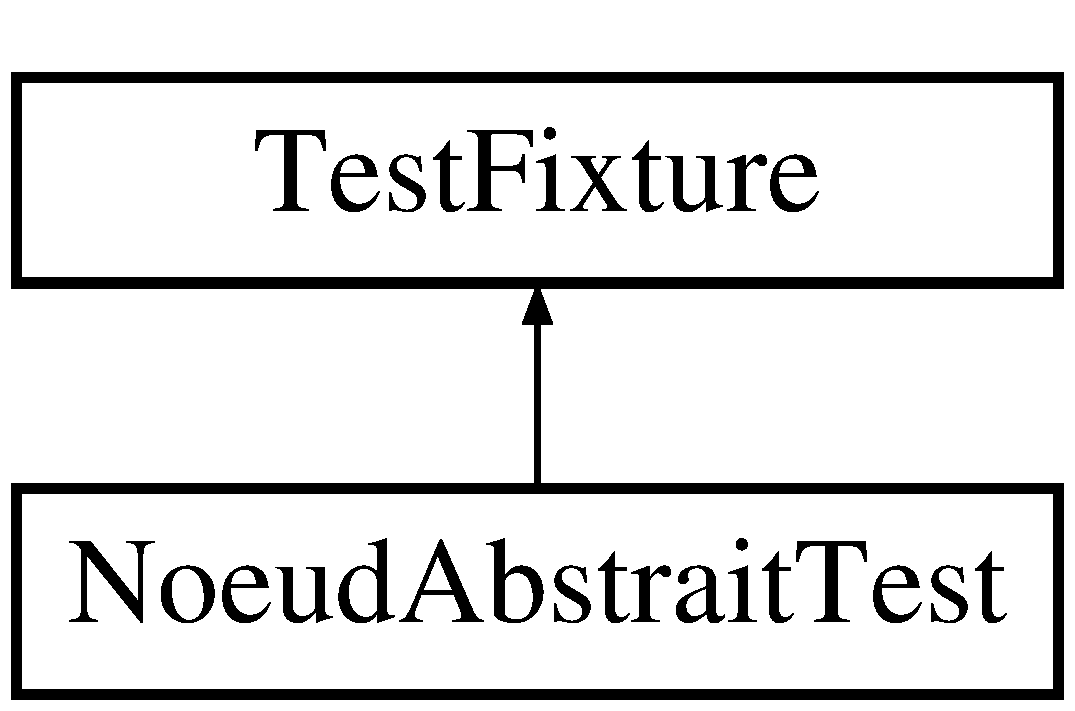
\includegraphics[height=2.000000cm]{class_noeud_abstrait_test}
\end{center}
\end{figure}
\subsection*{Public Member Functions}
\begin{DoxyCompactItemize}
\item 
void \hyperlink{group__inf2990_ga4d2fe388f550ba374823d09b5c8ebe77}{set\+Up} ()
\begin{DoxyCompactList}\small\item\em Traitement � effectuer pour initialiser cette suite de tests. \end{DoxyCompactList}\item 
void \hyperlink{group__inf2990_ga2c5c558ff7e40386c724a55b670af417}{tear\+Down} ()
\begin{DoxyCompactList}\small\item\em Traitement � effectuer pour \textquotesingle{}finaliser\textquotesingle{} cette suite de tests. \end{DoxyCompactList}\item 
void \hyperlink{group__inf2990_gaed7a5423d2a3a7518aef743f17d32ccd}{test\+Position\+Relative} ()
\begin{DoxyCompactList}\small\item\em Cas de test\+: �criture/lecture de la position relative. \end{DoxyCompactList}\item 
void \hyperlink{group__inf2990_gadf554a62266cc21c7c48f6a27ad7c752}{test\+Type} ()
\begin{DoxyCompactList}\small\item\em Cas de test\+: type de noeud. \end{DoxyCompactList}\item 
void \hyperlink{group__inf2990_gac044744b04574c86418a57b39e3238ff}{test\+Selection} ()
\begin{DoxyCompactList}\small\item\em Cas de test\+: d�finition/obtention des �tats de s�lection du noeud. \end{DoxyCompactList}\item 
void \hyperlink{group__inf2990_ga0e65b00620e79646a9efd8a93c4fc650}{test\+Enfants} ()
\begin{DoxyCompactList}\small\item\em Cas de test\+: s\textquotesingle{}assurer que le noeud abstrait n\textquotesingle{}a pas d\textquotesingle{}enfant. \end{DoxyCompactList}\end{DoxyCompactItemize}


\subsection{Detailed Description}
Classe de test cppunit pour tester le bon fonctionnement des m�thodes de la classe \hyperlink{class_noeud_abstrait}{Noeud\+Abstrait}. 

\begin{DoxyAuthor}{Author}
Julien Gascon-\/\+Samson 
\end{DoxyAuthor}
\begin{DoxyDate}{Date}
2011-\/07-\/16 
\end{DoxyDate}


The documentation for this class was generated from the following files\+:\begin{DoxyCompactItemize}
\item 
Sources/\+D\+L\+L/\+Tests/\hyperlink{_noeud_abstrait_test_8h}{Noeud\+Abstrait\+Test.\+h}\item 
Sources/\+D\+L\+L/\+Tests/\hyperlink{_noeud_abstrait_test_8cpp}{Noeud\+Abstrait\+Test.\+cpp}\end{DoxyCompactItemize}

\hypertarget{class_noeud_composite}{}\section{Noeud\+Composite Class Reference}
\label{class_noeud_composite}\index{Noeud\+Composite@{Noeud\+Composite}}


Implantation d\textquotesingle{}un noeud du patron composite qui peut poss�der des enfants.  




{\ttfamily \#include $<$Noeud\+Composite.\+h$>$}

Inheritance diagram for Noeud\+Composite\+:\begin{figure}[H]
\begin{center}
\leavevmode
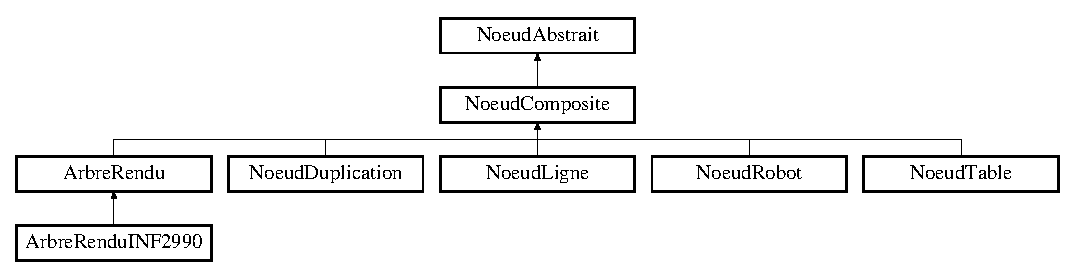
\includegraphics[height=3.270073cm]{class_noeud_composite}
\end{center}
\end{figure}
\subsection*{Public Member Functions}
\begin{DoxyCompactItemize}
\item 
\hyperlink{group__inf2990_ga49b3813ab1805b4b9e688ba0c4eaf56c}{Noeud\+Composite} (const std\+::string \&type=std\+::string\{\char`\"{}\char`\"{}\})
\begin{DoxyCompactList}\small\item\em Constructeur. \end{DoxyCompactList}\item 
virtual \hyperlink{group__inf2990_gaada4bd846bd950f2ac186b09f35aa9c6}{$\sim$\+Noeud\+Composite} ()
\begin{DoxyCompactList}\small\item\em Destructeur. \end{DoxyCompactList}\item 
virtual unsigned int \hyperlink{group__inf2990_gac2725a10b80438f67bb51076f13a78e1}{calculer\+Profondeur} () const 
\begin{DoxyCompactList}\small\item\em Calcule la profondeur de l\textquotesingle{}arbre sous le noeud courant. \end{DoxyCompactList}\item 
virtual void \hyperlink{group__inf2990_ga5e1564f2f07f5cd84cef7078ae88e3c6}{vider} ()
\begin{DoxyCompactList}\small\item\em Vide le noeud de ses enfants. \end{DoxyCompactList}\item 
virtual void \hyperlink{group__inf2990_gabdc10574cb2b5c4825bc10b610fa9b5d}{effacer} (const \hyperlink{class_noeud_abstrait}{Noeud\+Abstrait} $\ast$noeud)
\begin{DoxyCompactList}\small\item\em Efface le noeud pass� en param�tre. \end{DoxyCompactList}\item 
virtual const \hyperlink{class_noeud_abstrait}{Noeud\+Abstrait} $\ast$ \hyperlink{group__inf2990_ga3bc273d5a3b1aed9e697bd2fa540403d}{chercher} (const std\+::string \&type\+Noeud) const 
\begin{DoxyCompactList}\small\item\em Cherche un noeud par le type (sur un noeud constant). \end{DoxyCompactList}\item 
virtual \hyperlink{class_noeud_abstrait}{Noeud\+Abstrait} $\ast$ \hyperlink{group__inf2990_ga622dcce31cdfb05afeedb7602e007f25}{chercher} (const std\+::string \&type\+Noeud)
\begin{DoxyCompactList}\small\item\em Cherche un noeud par le type. \end{DoxyCompactList}\item 
virtual const \hyperlink{class_noeud_abstrait}{Noeud\+Abstrait} $\ast$ \hyperlink{group__inf2990_gacf157b0fc2a929cc8e711dba2e201660}{chercher} (unsigned int indice) const 
\begin{DoxyCompactList}\small\item\em Cherche un noeud enfant selon l\textquotesingle{}indice (sur un noeud constant). \end{DoxyCompactList}\item 
virtual \hyperlink{class_noeud_abstrait}{Noeud\+Abstrait} $\ast$ \hyperlink{group__inf2990_ga67f24432c3a667154adf005f2c6c4396}{chercher} (unsigned int indice)
\begin{DoxyCompactList}\small\item\em Cherche un noeud enfant selon l\textquotesingle{}indice. \end{DoxyCompactList}\item 
virtual bool \hyperlink{group__inf2990_gaa9223c6e75378880678c8f6f5bc614ef}{ajouter} (std\+::shared\+\_\+ptr$<$ \hyperlink{class_noeud_abstrait}{Noeud\+Abstrait} $>$ enfant)
\begin{DoxyCompactList}\small\item\em Ajoute un noeud enfant. \end{DoxyCompactList}\item 
virtual unsigned int \hyperlink{group__inf2990_ga87b0010b4dc77c69c6114a70f3de73bd}{obtenir\+Nombre\+Enfants} () const 
\begin{DoxyCompactList}\small\item\em Obtient le nombre d\textquotesingle{}enfants du noeud. \end{DoxyCompactList}\item 
virtual void \hyperlink{group__inf2990_ga64bcef79a467ea669275d885dbe31c8d}{effacer\+Selection} ()
\begin{DoxyCompactList}\small\item\em Efface les enfants s�lectionn�s. \end{DoxyCompactList}\item 
virtual void \hyperlink{group__inf2990_ga6c0620784aa50cb5c19664124e884cdd}{selectionner\+Tout} ()
\begin{DoxyCompactList}\small\item\em S�lectionne tous les enfants de m�me que le noeud. \end{DoxyCompactList}\item 
virtual void \hyperlink{group__inf2990_ga0a838e8f0a086e71856e3a116508bcf2}{deselectionner\+Tout} ()
\begin{DoxyCompactList}\small\item\em D�s�lectionne tous les enfants de m�me que le noeud. \end{DoxyCompactList}\item 
virtual bool \hyperlink{group__inf2990_ga38f910a0d19bb3d091daa285ad91cd8a}{selection\+Existe} () const 
\begin{DoxyCompactList}\small\item\em V�rifier si le noeud ou un de ses enfants est s�lectionn�. \end{DoxyCompactList}\item 
virtual void \hyperlink{group__inf2990_gafcbaa01f832fc2dad13b363253963d0b}{changer\+Mode\+Polygones} (bool est\+Force)
\begin{DoxyCompactList}\small\item\em Change le mode d\textquotesingle{}affichage des polygones. \end{DoxyCompactList}\item 
virtual void \hyperlink{group__inf2990_gaeeeca055ef6aef0435b9956eb467ff7f}{assigner\+Mode\+Polygones} (G\+Lenum mode\+Polygones)
\begin{DoxyCompactList}\small\item\em Assigne le mode d\textquotesingle{}affichage des polygones. \end{DoxyCompactList}\item 
virtual void \hyperlink{group__inf2990_gad440d00734a92e1bd99cdee2ac62bb68}{afficher\+Concret} () const 
\begin{DoxyCompactList}\small\item\em Affiche le noeud de mani�re concr�te. \end{DoxyCompactList}\item 
virtual void \hyperlink{group__inf2990_ga57f31e1a0fd79628d04651001014fd41}{animer} (float dt)
\begin{DoxyCompactList}\small\item\em Anime le noeud. \end{DoxyCompactList}\item 
std\+::shared\+\_\+ptr$<$ const \hyperlink{class_noeud_abstrait}{Noeud\+Abstrait} $>$ \hyperlink{group__inf2990_gab5bab976c7d2ff3ba8a9b6cb5aaab337}{get\+Enfant} (int indice) const 
\item 
std\+::vector$<$ std\+::shared\+\_\+ptr$<$ \hyperlink{class_noeud_abstrait}{Noeud\+Abstrait} $>$ $>$ \& \hyperlink{group__inf2990_gad43a84360f8bcb25e65dcd6ad7c617f6}{get\+Enfants} ()
\end{DoxyCompactItemize}
\subsection*{Protected Types}
\begin{DoxyCompactItemize}
\item 
using \hyperlink{class_noeud_composite_a431d7ef6aa37ab91688cd2792d9a9b78}{conteneur\+\_\+enfants} = std\+::vector$<$ std\+::shared\+\_\+ptr$<$ \hyperlink{class_noeud_abstrait}{Noeud\+Abstrait} $>$$>$\hypertarget{class_noeud_composite_a431d7ef6aa37ab91688cd2792d9a9b78}{}\label{class_noeud_composite_a431d7ef6aa37ab91688cd2792d9a9b78}

\begin{DoxyCompactList}\small\item\em Le choix du conteneur pour les enfants. \end{DoxyCompactList}\end{DoxyCompactItemize}
\subsection*{Protected Attributes}
\begin{DoxyCompactItemize}
\item 
\hyperlink{class_noeud_composite_a431d7ef6aa37ab91688cd2792d9a9b78}{conteneur\+\_\+enfants} \hyperlink{class_noeud_composite_a628227fd324020e497ada7577457ff3f}{enfants\+\_\+}\hypertarget{class_noeud_composite_a628227fd324020e497ada7577457ff3f}{}\label{class_noeud_composite_a628227fd324020e497ada7577457ff3f}

\begin{DoxyCompactList}\small\item\em La liste des enfants. \end{DoxyCompactList}\end{DoxyCompactItemize}


\subsection{Detailed Description}
Implantation d\textquotesingle{}un noeud du patron composite qui peut poss�der des enfants. 

Cette classe implante les diff�rentes fonctions relatives aux enfants, comme l\textquotesingle{}ajout, le retrait, la recherche, etc.

\begin{DoxyAuthor}{Author}
D\+G\+I-\/2990 
\end{DoxyAuthor}
\begin{DoxyDate}{Date}
2007-\/01-\/24 
\end{DoxyDate}


The documentation for this class was generated from the following files\+:\begin{DoxyCompactItemize}
\item 
Sources/\+D\+L\+L/\+Arbre/\+Noeuds/\hyperlink{_noeud_composite_8h}{Noeud\+Composite.\+h}\item 
Sources/\+D\+L\+L/\+Arbre/\+Noeuds/\hyperlink{_noeud_composite_8cpp}{Noeud\+Composite.\+cpp}\end{DoxyCompactItemize}

\hypertarget{class_noeud_depart}{}\section{Noeud\+Depart Class Reference}
\label{class_noeud_depart}\index{Noeud\+Depart@{Noeud\+Depart}}


Classe qui repr�sente le point d�part du robot lors de la simulation.  




{\ttfamily \#include $<$Noeud\+Depart.\+h$>$}

Inheritance diagram for Noeud\+Depart\+:\begin{figure}[H]
\begin{center}
\leavevmode
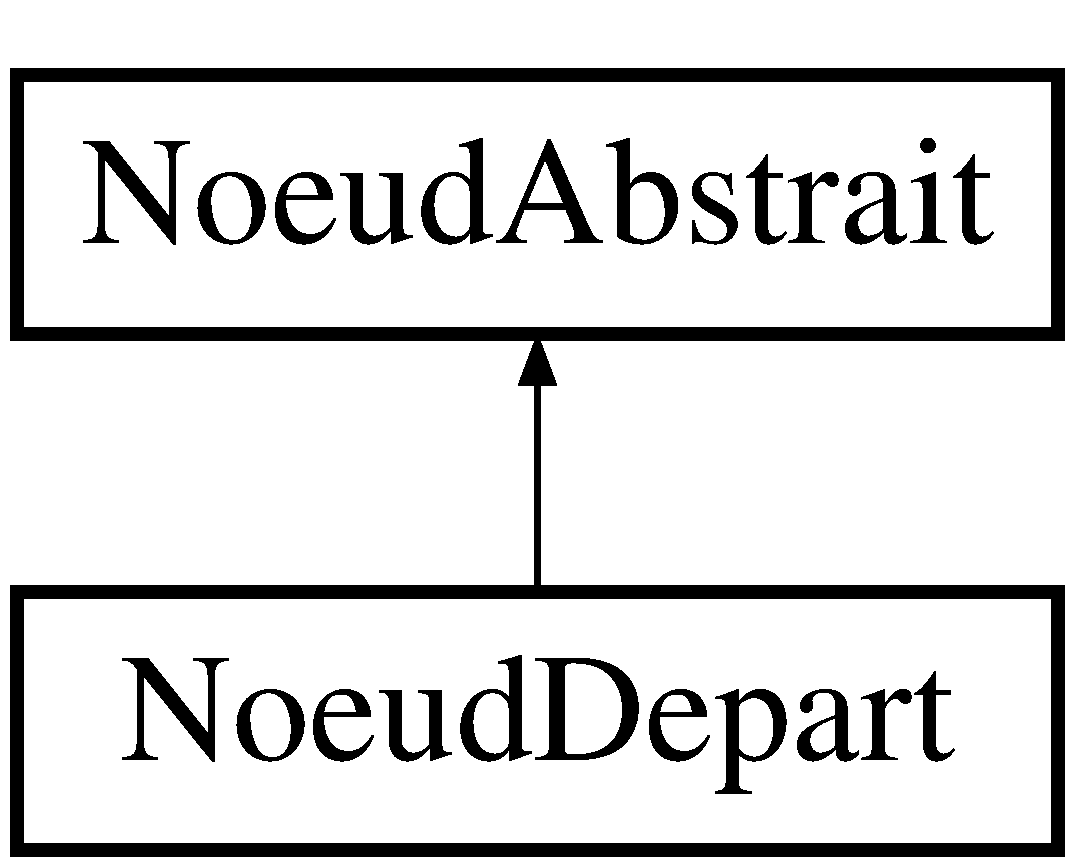
\includegraphics[height=2.000000cm]{class_noeud_depart}
\end{center}
\end{figure}
\subsection*{Public Member Functions}
\begin{DoxyCompactItemize}
\item 
\hyperlink{group__inf2990_ga003d2fbed3f4e142a9187a8152a4663d}{Noeud\+Depart} (const std\+::string \&type\+Noeud)
\begin{DoxyCompactList}\small\item\em Constructeur � partir du type du noeud. \end{DoxyCompactList}\item 
\hyperlink{group__inf2990_gab892d451fa06fb1de23da2884dcff8c4}{$\sim$\+Noeud\+Depart} ()
\begin{DoxyCompactList}\small\item\em Destructeur. \end{DoxyCompactList}\item 
virtual void \hyperlink{group__inf2990_ga2486360c54ec059d6a594d9dd9f691b4}{afficher\+Concret} () const 
\begin{DoxyCompactList}\small\item\em Affiche la table. \end{DoxyCompactList}\item 
virtual void \hyperlink{group__inf2990_gaa171386bd2c4687d59ea48a3321b5209}{accepter\+Visiteur} (\hyperlink{class_visiteur_abstrait}{Visiteur\+Abstrait} $\ast$visiteur)
\end{DoxyCompactItemize}
\subsection*{Additional Inherited Members}


\subsection{Detailed Description}
Classe qui repr�sente le point d�part du robot lors de la simulation. 

\begin{DoxyAuthor}{Author}
Fr�d�ric Gr�goire 
\end{DoxyAuthor}
\begin{DoxyDate}{Date}
2015-\/08-\/30 
\end{DoxyDate}


The documentation for this class was generated from the following files\+:\begin{DoxyCompactItemize}
\item 
Sources/\+D\+L\+L/\+Arbre/\+Noeuds/\hyperlink{_noeud_depart_8h}{Noeud\+Depart.\+h}\item 
Sources/\+D\+L\+L/\+Arbre/\+Noeuds/\hyperlink{_noeud_depart_8cpp}{Noeud\+Depart.\+cpp}\item 
Sources/\+D\+L\+L/\+Arbre/\+Noeuds/\hyperlink{_noeud_duplication_8cpp}{Noeud\+Duplication.\+cpp}\end{DoxyCompactItemize}

\hypertarget{class_noeud_duplication}{}\section{Noeud\+Duplication Class Reference}
\label{class_noeud_duplication}\index{Noeud\+Duplication@{Noeud\+Duplication}}


Noeud qui repr�sente une duplication lors de l\textquotesingle{}utilisation de l\textquotesingle{}outil duplication.  




{\ttfamily \#include $<$Noeud\+Duplication.\+h$>$}

Inheritance diagram for Noeud\+Duplication\+:\begin{figure}[H]
\begin{center}
\leavevmode
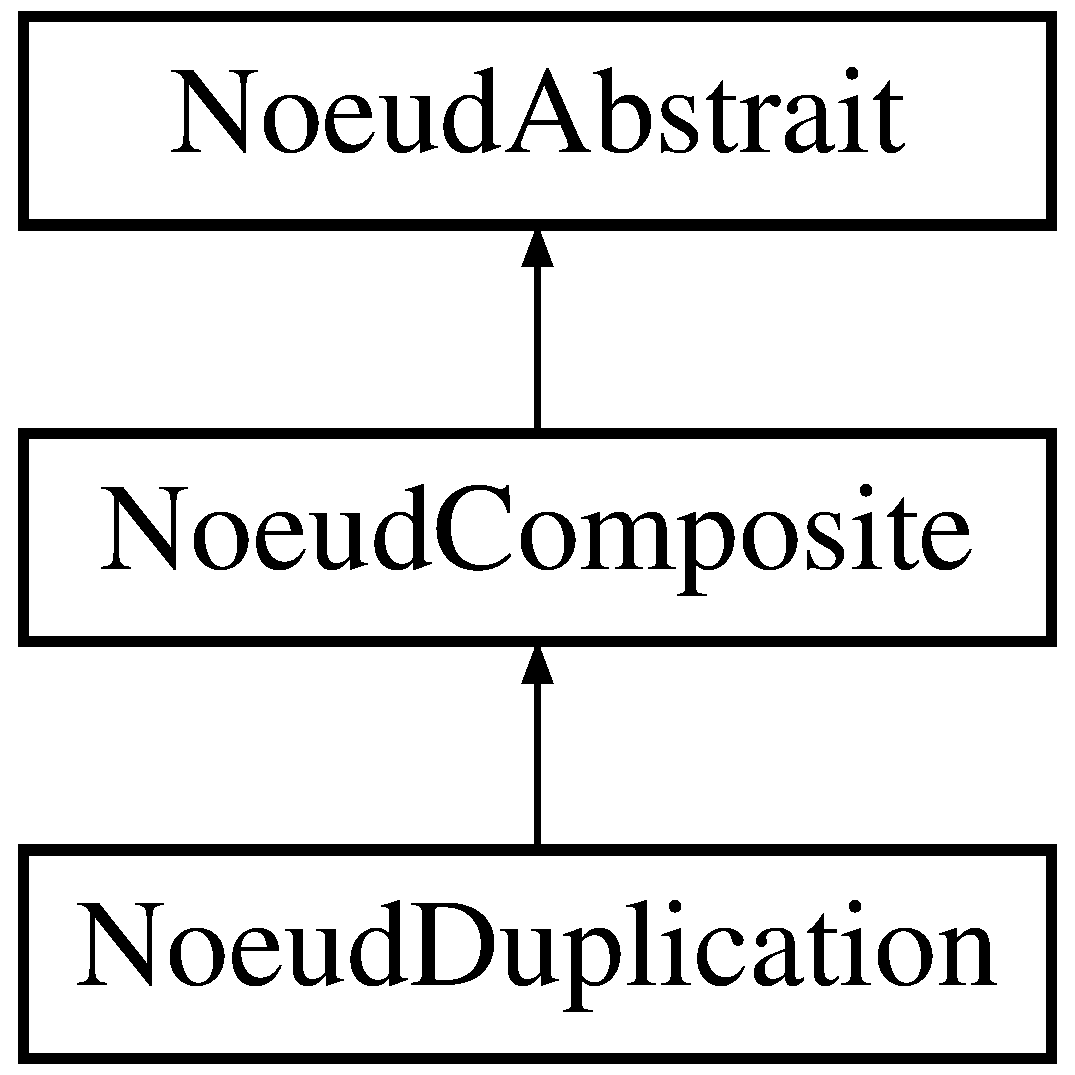
\includegraphics[height=3.000000cm]{class_noeud_duplication}
\end{center}
\end{figure}
\subsection*{Public Member Functions}
\begin{DoxyCompactItemize}
\item 
\hyperlink{group__inf2990_gafe5471984f6f9805abc4e39c64b494fe}{Noeud\+Duplication} (const std\+::string \&type\+Noeud)
\begin{DoxyCompactList}\small\item\em Constructeur. \end{DoxyCompactList}\item 
\hyperlink{group__inf2990_gab52b2f978fac8e9654fd4812f97aa76d}{$\sim$\+Noeud\+Duplication} ()
\begin{DoxyCompactList}\small\item\em Destructeur. \end{DoxyCompactList}\item 
virtual void \hyperlink{group__inf2990_gabfd08f04600651e5fd4a5bd9bda80564}{afficher\+Concret} () const 
\begin{DoxyCompactList}\small\item\em Affiche la table. \end{DoxyCompactList}\item 
std\+::shared\+\_\+ptr$<$ \hyperlink{class_noeud_abstrait}{Noeud\+Abstrait} $>$ \hyperlink{group__inf2990_ga031650073b688ab1baa3098c9a9356ef}{obtenir\+Duplication} (const int \&indice)
\begin{DoxyCompactList}\small\item\em Obtenir le pointeur intelligent d\textquotesingle{}un noeud dans le but de faire un transfert de possession. \end{DoxyCompactList}\item 
virtual void \hyperlink{group__inf2990_gaa3bf13e56a52b28b5c21aa5a0d028589}{accepter\+Visiteur} (\hyperlink{class_visiteur_abstrait}{Visiteur\+Abstrait} $\ast$visiteur)
\end{DoxyCompactItemize}
\subsection*{Additional Inherited Members}


\subsection{Detailed Description}
Noeud qui repr�sente une duplication lors de l\textquotesingle{}utilisation de l\textquotesingle{}outil duplication. 

\begin{DoxyAuthor}{Author}
Olivier St-\/\+Amour 
\end{DoxyAuthor}
\begin{DoxyDate}{Date}
2016-\/02-\/15 
\end{DoxyDate}


The documentation for this class was generated from the following files\+:\begin{DoxyCompactItemize}
\item 
Sources/\+D\+L\+L/\+Arbre/\+Noeuds/\hyperlink{_noeud_duplication_8h}{Noeud\+Duplication.\+h}\item 
Sources/\+D\+L\+L/\+Arbre/\+Noeuds/\hyperlink{_noeud_duplication_8cpp}{Noeud\+Duplication.\+cpp}\end{DoxyCompactItemize}

\hypertarget{class_noeud_jonction}{}\section{Noeud\+Jonction Class Reference}
\label{class_noeud_jonction}\index{Noeud\+Jonction@{Noeud\+Jonction}}


Noeud de l\textquotesingle{}objet rendu servant � la liaison de segments de la ligne noire.  




{\ttfamily \#include $<$Noeud\+Jonction.\+h$>$}

Inheritance diagram for Noeud\+Jonction\+:\begin{figure}[H]
\begin{center}
\leavevmode
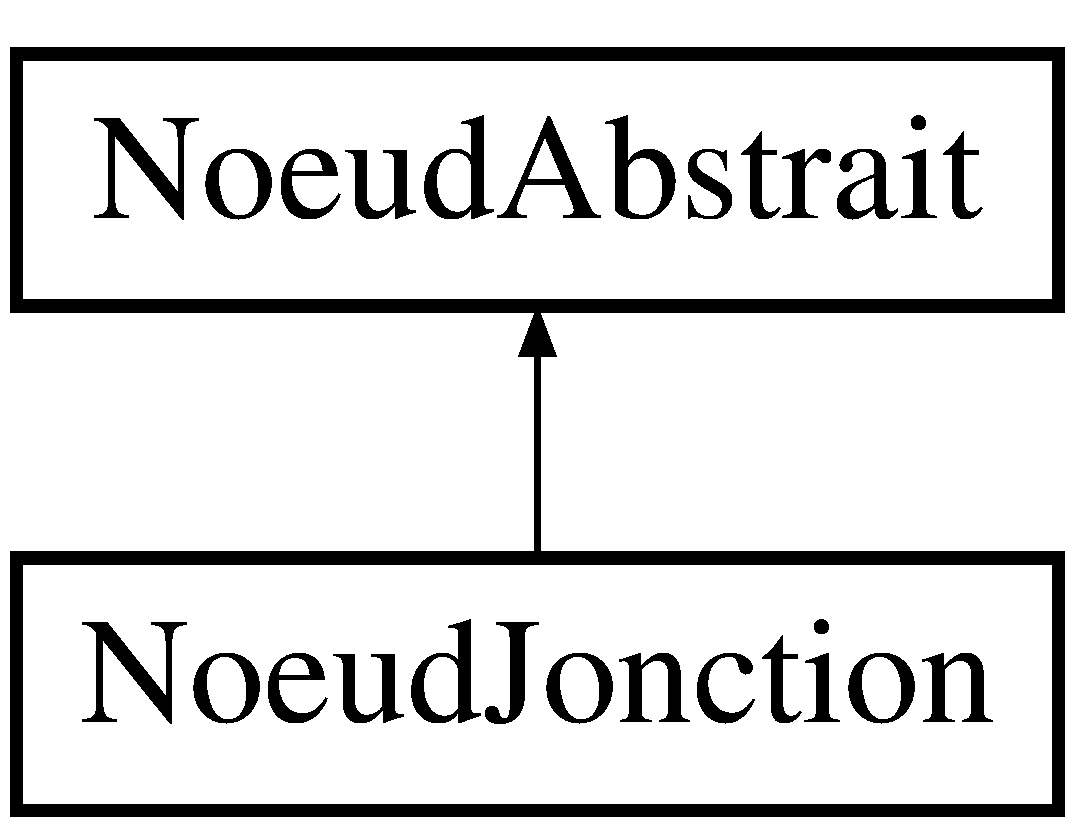
\includegraphics[height=2.000000cm]{class_noeud_jonction}
\end{center}
\end{figure}
\subsection*{Public Member Functions}
\begin{DoxyCompactItemize}
\item 
\hyperlink{group__inf2990_ga5b516af4920b0a32f19d39bd3784cf18}{Noeud\+Jonction} (const std\+::string \&type\+Noeud)
\begin{DoxyCompactList}\small\item\em Constructeur. \end{DoxyCompactList}\item 
\hyperlink{group__inf2990_ga6d18cdb62fd0daf6321715451bf7ca8e}{$\sim$\+Noeud\+Jonction} ()
\begin{DoxyCompactList}\small\item\em Destructeur. \end{DoxyCompactList}\item 
virtual void \hyperlink{group__inf2990_gac33360e21e68b6774cc9de0fd71506ed}{afficher\+Concret} () const 
\begin{DoxyCompactList}\small\item\em Affiche la table. \end{DoxyCompactList}\item 
virtual void \hyperlink{group__inf2990_ga46f3e689e30090973acbe592c34fb8d4}{accepter\+Visiteur} (\hyperlink{class_visiteur_abstrait}{Visiteur\+Abstrait} $\ast$visiteur)
\end{DoxyCompactItemize}
\subsection*{Additional Inherited Members}


\subsection{Detailed Description}
Noeud de l\textquotesingle{}objet rendu servant � la liaison de segments de la ligne noire. 

\begin{DoxyAuthor}{Author}
Camille Gendreau 
\end{DoxyAuthor}
\begin{DoxyDate}{Date}
2007-\/01-\/24 
\end{DoxyDate}


The documentation for this class was generated from the following files\+:\begin{DoxyCompactItemize}
\item 
Sources/\+D\+L\+L/\+Arbre/\+Noeuds/\hyperlink{_noeud_jonction_8h}{Noeud\+Jonction.\+h}\item 
Sources/\+D\+L\+L/\+Arbre/\+Noeuds/Noeud\+Jonction.\+cpp\end{DoxyCompactItemize}

\hypertarget{class_noeud_ligne}{}\section{Noeud\+Ligne Class Reference}
\label{class_noeud_ligne}\index{Noeud\+Ligne@{Noeud\+Ligne}}


Noeud de l\textquotesingle{}objet englobant tous les segments et jonctions d\textquotesingle{}une ligne noire.  




{\ttfamily \#include $<$Noeud\+Ligne.\+h$>$}

Inheritance diagram for Noeud\+Ligne\+:\begin{figure}[H]
\begin{center}
\leavevmode
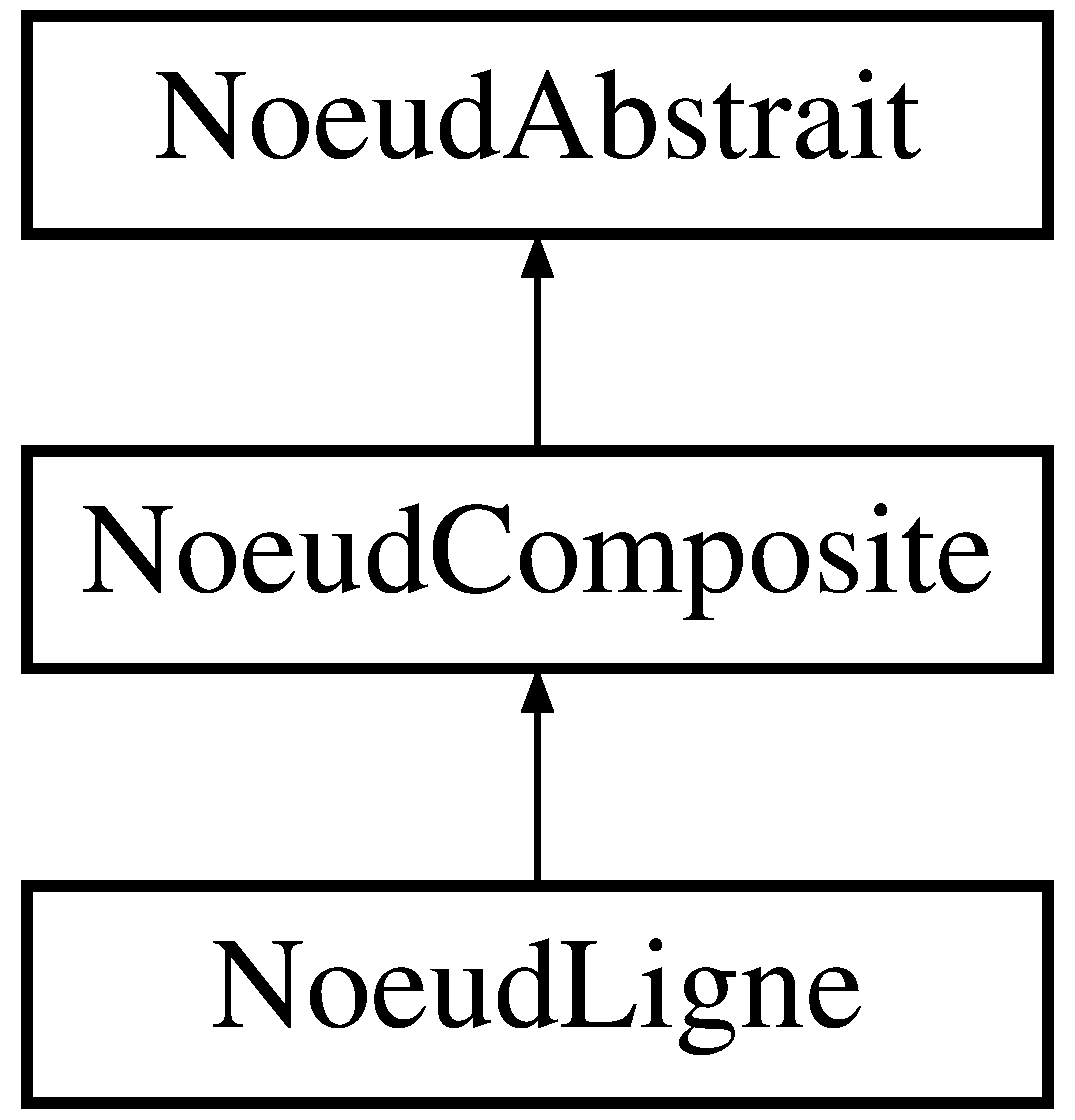
\includegraphics[height=3.000000cm]{class_noeud_ligne}
\end{center}
\end{figure}
\subsection*{Public Member Functions}
\begin{DoxyCompactItemize}
\item 
\hyperlink{group__inf2990_gae8bead463f4616abc90d29923226a92f}{Noeud\+Ligne} (const std\+::string \&type\+Noeud)
\begin{DoxyCompactList}\small\item\em Constructeur. \end{DoxyCompactList}\item 
\hyperlink{group__inf2990_ga5bbf8d24a63e0370aa8666f401f36599}{$\sim$\+Noeud\+Ligne} ()
\begin{DoxyCompactList}\small\item\em Destructeur. \end{DoxyCompactList}\item 
virtual void \hyperlink{group__inf2990_ga727a134065eeb6b101ad020a15a92a19}{afficher\+Concret} () const 
\begin{DoxyCompactList}\small\item\em Affiche la table. \end{DoxyCompactList}\item 
virtual void \hyperlink{group__inf2990_ga16d9aaa3cd21305ec6f91ad5442132f0}{accepter\+Visiteur} (\hyperlink{class_visiteur_abstrait}{Visiteur\+Abstrait} $\ast$visiteur)
\end{DoxyCompactItemize}
\subsection*{Additional Inherited Members}


\subsection{Detailed Description}
Noeud de l\textquotesingle{}objet englobant tous les segments et jonctions d\textquotesingle{}une ligne noire. 

Noeud des murs servant d\textquotesingle{}obstacles au robot.

\begin{DoxyAuthor}{Author}

\end{DoxyAuthor}
\begin{DoxyDate}{Date}
2016-\/01-\/20
\end{DoxyDate}
\begin{DoxyAuthor}{Author}
Fr�d�ric Gr�goire 
\end{DoxyAuthor}
\begin{DoxyDate}{Date}
2016-\/01-\/20 
\end{DoxyDate}


The documentation for this class was generated from the following files\+:\begin{DoxyCompactItemize}
\item 
Sources/\+D\+L\+L/\+Arbre/\+Noeuds/\hyperlink{_noeud_ligne_8h}{Noeud\+Ligne.\+h}\item 
Sources/\+D\+L\+L/\+Arbre/\+Noeuds/\hyperlink{_noeud_ligne_8cpp}{Noeud\+Ligne.\+cpp}\end{DoxyCompactItemize}

\hypertarget{class_noeud_mur}{}\section{Noeud\+Mur Class Reference}
\label{class_noeud_mur}\index{Noeud\+Mur@{Noeud\+Mur}}
Inheritance diagram for Noeud\+Mur\+:\begin{figure}[H]
\begin{center}
\leavevmode
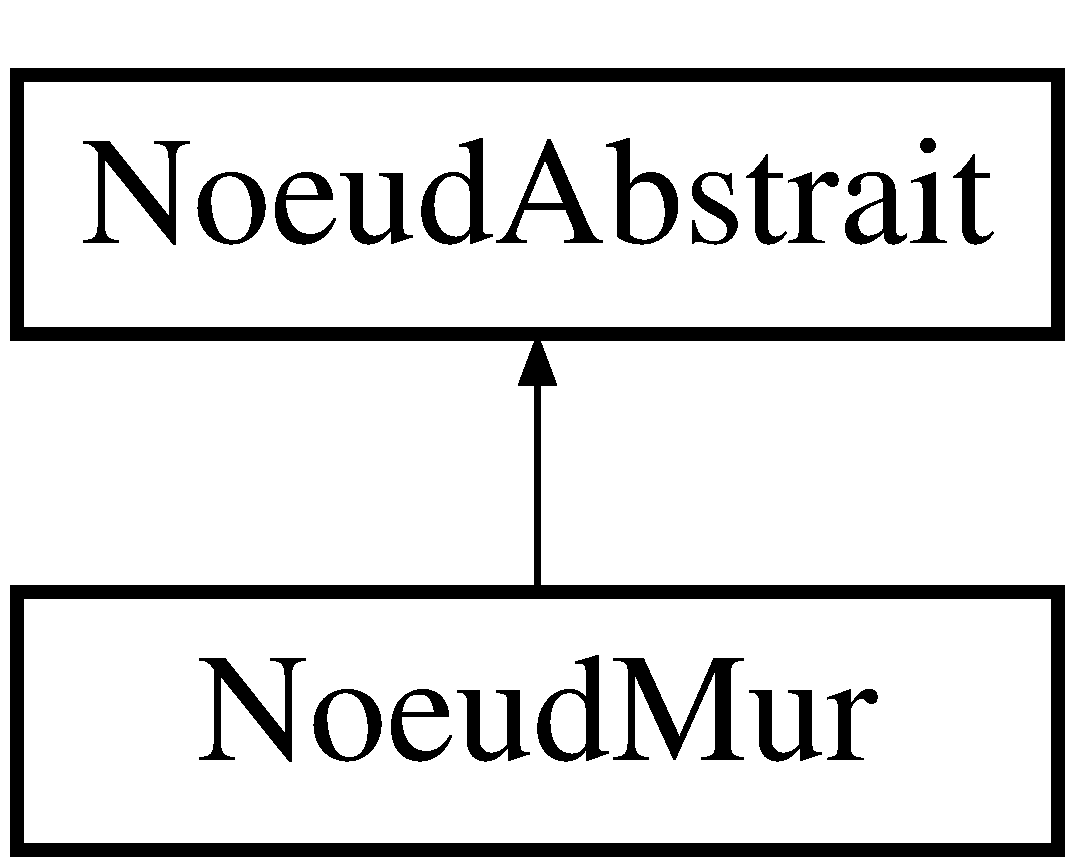
\includegraphics[height=2.000000cm]{class_noeud_mur}
\end{center}
\end{figure}
\subsection*{Public Member Functions}
\begin{DoxyCompactItemize}
\item 
\hyperlink{group__inf2990_gaeab2deec90548c0bdca5eb86beb629cf}{Noeud\+Mur} (const std\+::string \&type\+Noeud)
\begin{DoxyCompactList}\small\item\em Constructeur. \end{DoxyCompactList}\item 
\hyperlink{group__inf2990_ga169060e04a6423e7f025d475afd7d9ea}{$\sim$\+Noeud\+Mur} ()
\begin{DoxyCompactList}\small\item\em Destructeur. \end{DoxyCompactList}\item 
virtual void \hyperlink{group__inf2990_ga521a3062875ea6ed1645485412a70c7b}{afficher\+Concret} () const 
\begin{DoxyCompactList}\small\item\em Affiche la table. \end{DoxyCompactList}\item 
virtual void \hyperlink{group__inf2990_ga91ea1a5930052142e26a359fd5bf9828}{accepter\+Visiteur} (\hyperlink{class_visiteur_abstrait}{Visiteur\+Abstrait} $\ast$visiteur)
\end{DoxyCompactItemize}
\subsection*{Additional Inherited Members}


The documentation for this class was generated from the following files\+:\begin{DoxyCompactItemize}
\item 
Sources/\+D\+L\+L/\+Arbre/\+Noeuds/\hyperlink{_noeud_mur_8h}{Noeud\+Mur.\+h}\item 
Sources/\+D\+L\+L/\+Arbre/\+Noeuds/\hyperlink{_noeud_mur_8cpp}{Noeud\+Mur.\+cpp}\end{DoxyCompactItemize}

\hypertarget{class_noeud_poteau}{}\section{Noeud\+Poteau Class Reference}
\label{class_noeud_poteau}\index{Noeud\+Poteau@{Noeud\+Poteau}}


Noeud des obstacles au robot sous forme de poteaux.  




{\ttfamily \#include $<$Noeud\+Poteau.\+h$>$}

Inheritance diagram for Noeud\+Poteau\+:\begin{figure}[H]
\begin{center}
\leavevmode
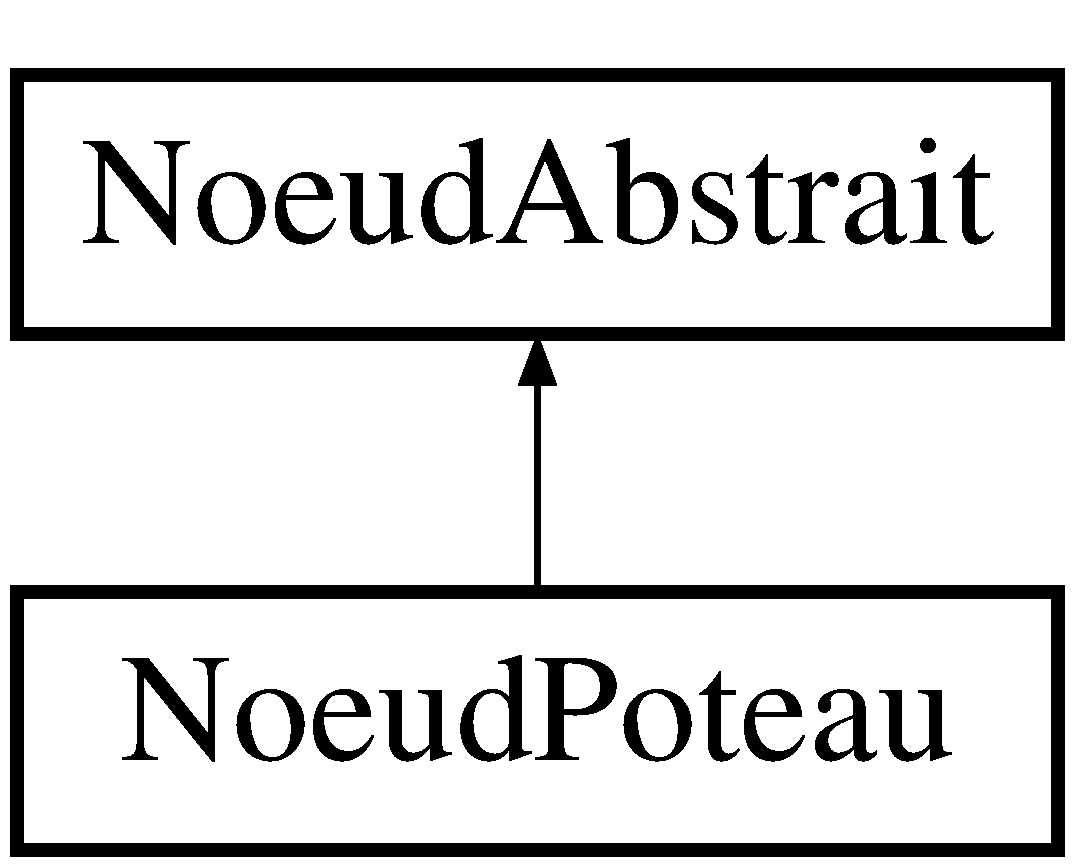
\includegraphics[height=2.000000cm]{class_noeud_poteau}
\end{center}
\end{figure}
\subsection*{Public Member Functions}
\begin{DoxyCompactItemize}
\item 
\hyperlink{group__inf2990_ga6c9d4922b38056bd9f6dfc4404c76932}{Noeud\+Poteau} (const std\+::string \&type\+Noeud)
\begin{DoxyCompactList}\small\item\em Constructeur. \end{DoxyCompactList}\item 
\hyperlink{group__inf2990_ga19737d5053bd375435d9f3c55482a695}{$\sim$\+Noeud\+Poteau} ()
\begin{DoxyCompactList}\small\item\em Destructeur. \end{DoxyCompactList}\item 
virtual void \hyperlink{group__inf2990_gaa637c540c30272bbe3404625d00bb4e8}{afficher\+Concret} () const 
\begin{DoxyCompactList}\small\item\em Affiche la table. \end{DoxyCompactList}\item 
virtual void \hyperlink{group__inf2990_ga7b28ff37ea5f58733652ab2f2ec55669}{accepter\+Visiteur} (\hyperlink{class_visiteur_abstrait}{Visiteur\+Abstrait} $\ast$visiteur)
\end{DoxyCompactItemize}
\subsection*{Additional Inherited Members}


\subsection{Detailed Description}
Noeud des obstacles au robot sous forme de poteaux. 

\begin{DoxyAuthor}{Author}
Fr�d�ric Gr�goire 
\end{DoxyAuthor}
\begin{DoxyDate}{Date}
2016-\/01-\/20 
\end{DoxyDate}


The documentation for this class was generated from the following files\+:\begin{DoxyCompactItemize}
\item 
Sources/\+D\+L\+L/\+Arbre/\+Noeuds/\hyperlink{_noeud_poteau_8h}{Noeud\+Poteau.\+h}\item 
Sources/\+D\+L\+L/\+Arbre/\+Noeuds/Noeud\+Jonction.\+cpp\item 
Sources/\+D\+L\+L/\+Arbre/\+Noeuds/\hyperlink{_noeud_poteau_8cpp}{Noeud\+Poteau.\+cpp}\end{DoxyCompactItemize}

\hypertarget{class_noeud_robot}{}\section{Noeud\+Robot Class Reference}
\label{class_noeud_robot}\index{Noeud\+Robot@{Noeud\+Robot}}


Classe qui repr�sente le robot du premier projet int�grateur.  




{\ttfamily \#include $<$Noeud\+Robot.\+h$>$}

Inheritance diagram for Noeud\+Robot\+:\begin{figure}[H]
\begin{center}
\leavevmode
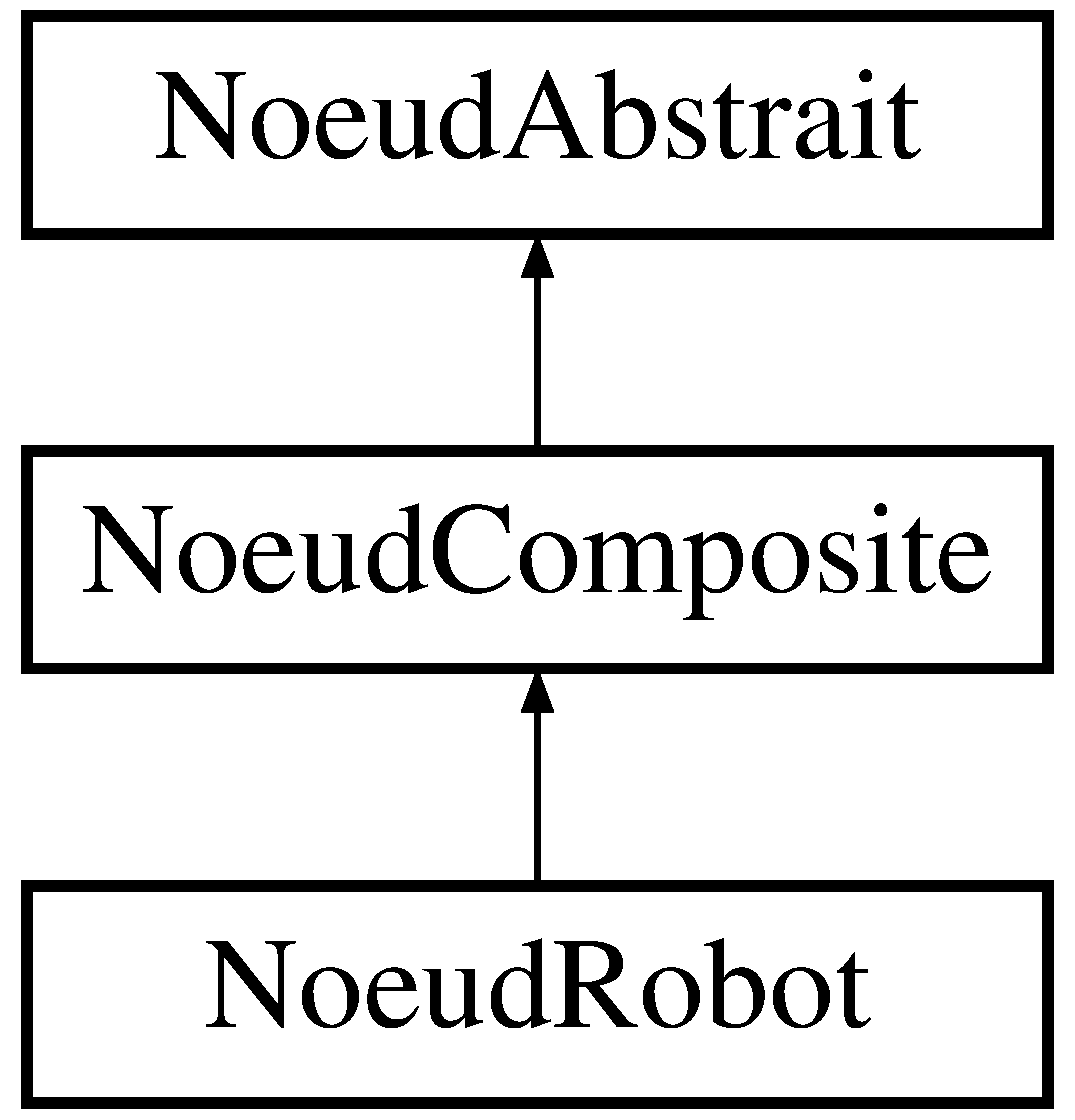
\includegraphics[height=3.000000cm]{class_noeud_robot}
\end{center}
\end{figure}
\subsection*{Public Member Functions}
\begin{DoxyCompactItemize}
\item 
\hyperlink{group__inf2990_ga147453ac7f72970d7d9bfe336998ad94}{Noeud\+Robot} (const std\+::string \&type\+Noeud)
\begin{DoxyCompactList}\small\item\em Constructeur � partir du type du noeud. \end{DoxyCompactList}\item 
\hyperlink{group__inf2990_ga5649710d151f0548d8a7a279aad4c655}{$\sim$\+Noeud\+Robot} ()
\begin{DoxyCompactList}\small\item\em Destructeur. \end{DoxyCompactList}\item 
virtual void \hyperlink{group__inf2990_gad63a8e09cc5ca8cc349f35e0901474e2}{afficher\+Concret} () const 
\begin{DoxyCompactList}\small\item\em Affiche le robot. \end{DoxyCompactList}\item 
virtual void \hyperlink{group__inf2990_ga6205113fc8bea6f9f43d39a1586e0dad}{accepter\+Visiteur} (\hyperlink{class_visiteur_abstrait}{Visiteur\+Abstrait} $\ast$visiteur)
\end{DoxyCompactItemize}
\subsection*{Additional Inherited Members}


\subsection{Detailed Description}
Classe qui repr�sente le robot du premier projet int�grateur. 

\begin{DoxyAuthor}{Author}
Martin Paradis 
\end{DoxyAuthor}
\begin{DoxyDate}{Date}
2015-\/08-\/30 
\end{DoxyDate}


The documentation for this class was generated from the following files\+:\begin{DoxyCompactItemize}
\item 
Sources/\+D\+L\+L/\+Arbre/\+Noeuds/\hyperlink{_noeud_robot_8h}{Noeud\+Robot.\+h}\item 
Sources/\+D\+L\+L/\+Arbre/\+Noeuds/\hyperlink{_noeud_robot_8cpp}{Noeud\+Robot.\+cpp}\end{DoxyCompactItemize}

\hypertarget{class_noeud_segment}{}\section{Noeud\+Segment Class Reference}
\label{class_noeud_segment}\index{Noeud\+Segment@{Noeud\+Segment}}


Chaque noeud de ce type repr�sente un des segments qui composent une ligne noire. Celles-\/ci se situent habituellement sous un objet de type \hyperlink{class_noeud_ligne}{Noeud\+Ligne}.  




{\ttfamily \#include $<$Noeud\+Segment.\+h$>$}

Inheritance diagram for Noeud\+Segment\+:\begin{figure}[H]
\begin{center}
\leavevmode
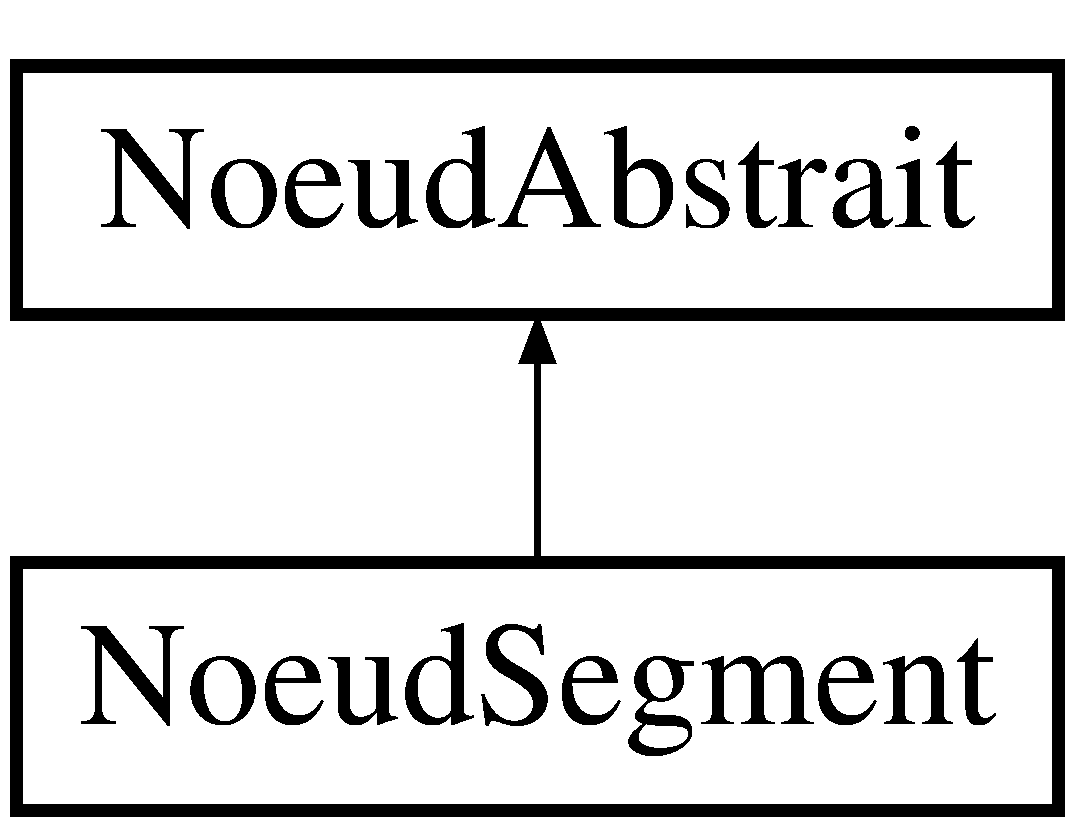
\includegraphics[height=2.000000cm]{class_noeud_segment}
\end{center}
\end{figure}
\subsection*{Public Member Functions}
\begin{DoxyCompactItemize}
\item 
\hyperlink{group__inf2990_ga10b40095ce1eec28d4ab46e01b2967f3}{Noeud\+Segment} (const std\+::string \&type\+Noeud)
\begin{DoxyCompactList}\small\item\em Constructeur. \end{DoxyCompactList}\item 
\hyperlink{group__inf2990_gad077426a22b964bb175e52a4090a13ac}{$\sim$\+Noeud\+Segment} ()
\begin{DoxyCompactList}\small\item\em Destructeur. \end{DoxyCompactList}\item 
virtual void \hyperlink{group__inf2990_ga0ba0aafc1352a0681bc9a90859795a20}{afficher\+Concret} () const 
\begin{DoxyCompactList}\small\item\em Affiche le segment. \end{DoxyCompactList}\item 
virtual void \hyperlink{group__inf2990_gadd01859fabe7b402a37563f5593c27b6}{accepter\+Visiteur} (\hyperlink{class_visiteur_abstrait}{Visiteur\+Abstrait} $\ast$visiteur)
\end{DoxyCompactItemize}
\subsection*{Additional Inherited Members}


\subsection{Detailed Description}
Chaque noeud de ce type repr�sente un des segments qui composent une ligne noire. Celles-\/ci se situent habituellement sous un objet de type \hyperlink{class_noeud_ligne}{Noeud\+Ligne}. 

\begin{DoxyAuthor}{Author}
Fr�d�ric Gr�goire 
\end{DoxyAuthor}
\begin{DoxyDate}{Date}
2016-\/01-\/20 
\end{DoxyDate}


The documentation for this class was generated from the following files\+:\begin{DoxyCompactItemize}
\item 
Sources/\+D\+L\+L/\+Arbre/\+Noeuds/Noeud\+Segment.\+h\item 
Sources/\+D\+L\+L/\+Arbre/\+Noeuds/\hyperlink{_noeud_segment_8cpp}{Noeud\+Segment.\+cpp}\end{DoxyCompactItemize}

\hypertarget{class_noeud_table}{}\section{Noeud\+Table Class Reference}
\label{class_noeud_table}\index{Noeud\+Table@{Noeud\+Table}}


Noeud repr�sentant la table, c\textquotesingle{}est � dire la zone de simulation.  




{\ttfamily \#include $<$Noeud\+Table.\+h$>$}

Inheritance diagram for Noeud\+Table\+:\begin{figure}[H]
\begin{center}
\leavevmode
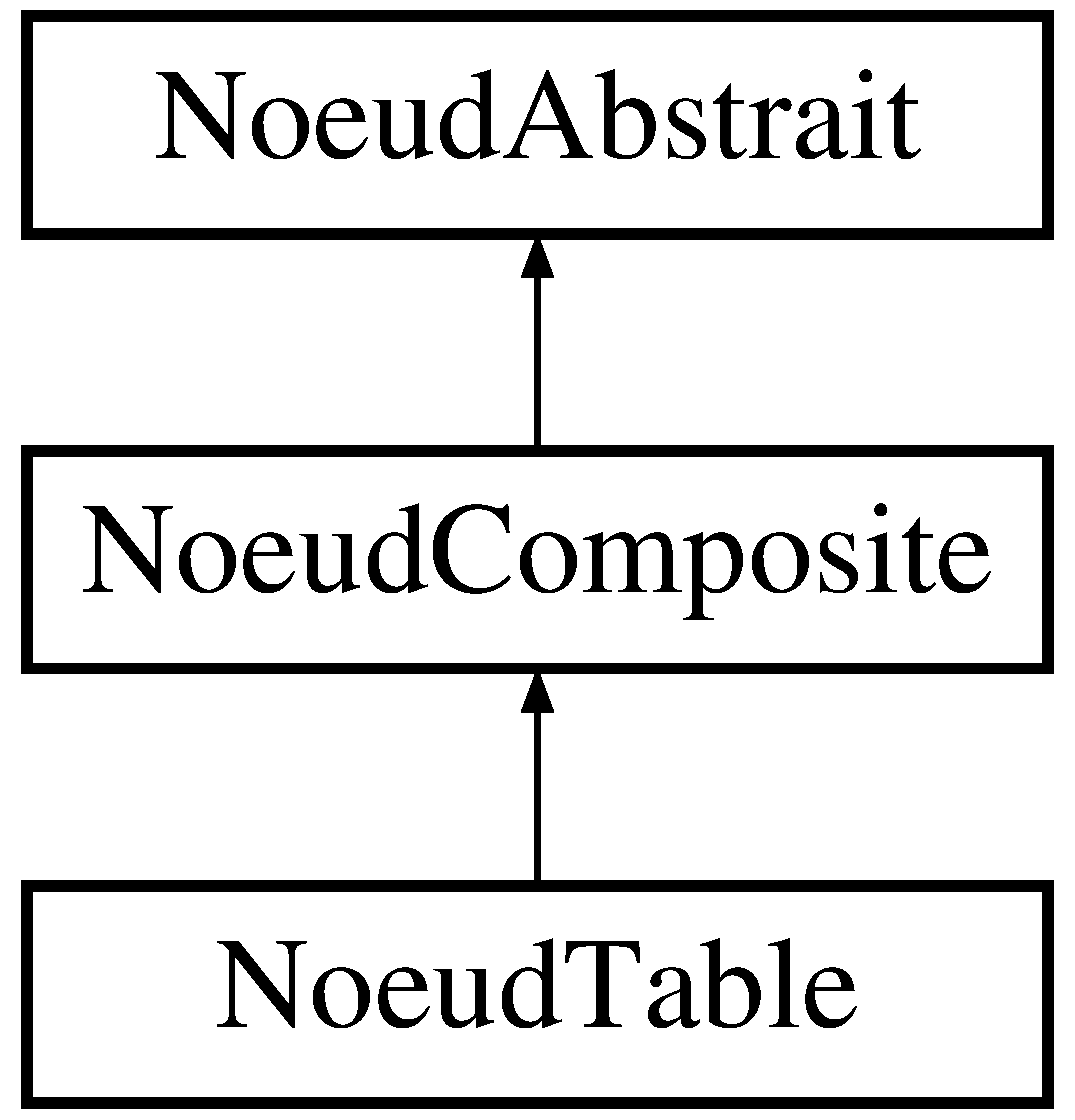
\includegraphics[height=3.000000cm]{class_noeud_table}
\end{center}
\end{figure}
\subsection*{Public Member Functions}
\begin{DoxyCompactItemize}
\item 
\hyperlink{group__inf2990_ga40983870720b331d17daeeb306e12ef5}{Noeud\+Table} (const std\+::string \&type\+Noeud)
\begin{DoxyCompactList}\small\item\em Constructeur. \end{DoxyCompactList}\item 
\hyperlink{group__inf2990_ga6171c2df59de6f454f0d8c7915403ce7}{$\sim$\+Noeud\+Table} ()
\begin{DoxyCompactList}\small\item\em Destructeur. \end{DoxyCompactList}\item 
virtual void \hyperlink{group__inf2990_gaa2876d070dd6fe57b0b90077fcd5036d}{afficher\+Concret} () const 
\begin{DoxyCompactList}\small\item\em Affiche la table. \end{DoxyCompactList}\item 
virtual void \hyperlink{group__inf2990_ga8fb25743b67de6b2186a687b5f2b4ffc}{accepter\+Visiteur} (\hyperlink{class_visiteur_abstrait}{Visiteur\+Abstrait} $\ast$visiteur)
\begin{DoxyCompactList}\small\item\em Accepter un visiteur. \end{DoxyCompactList}\end{DoxyCompactItemize}
\subsection*{Additional Inherited Members}


\subsection{Detailed Description}
Noeud repr�sentant la table, c\textquotesingle{}est � dire la zone de simulation. 

\begin{DoxyAuthor}{Author}
Camille Gendreau 
\end{DoxyAuthor}
\begin{DoxyDate}{Date}
2016-\/01-\/20 
\end{DoxyDate}


The documentation for this class was generated from the following files\+:\begin{DoxyCompactItemize}
\item 
Sources/\+D\+L\+L/\+Arbre/\+Noeuds/\hyperlink{_noeud_table_8h}{Noeud\+Table.\+h}\item 
Sources/\+D\+L\+L/\+Arbre/\+Noeuds/\hyperlink{_noeud_table_8cpp}{Noeud\+Table.\+cpp}\end{DoxyCompactItemize}

\hypertarget{class_interface_graphique_1_1_nouveau_fichier}{}\section{Interface\+Graphique.\+Nouveau\+Fichier Class Reference}
\label{class_interface_graphique_1_1_nouveau_fichier}\index{Interface\+Graphique.\+Nouveau\+Fichier@{Interface\+Graphique.\+Nouveau\+Fichier}}
Inheritance diagram for Interface\+Graphique.\+Nouveau\+Fichier\+:\begin{figure}[H]
\begin{center}
\leavevmode
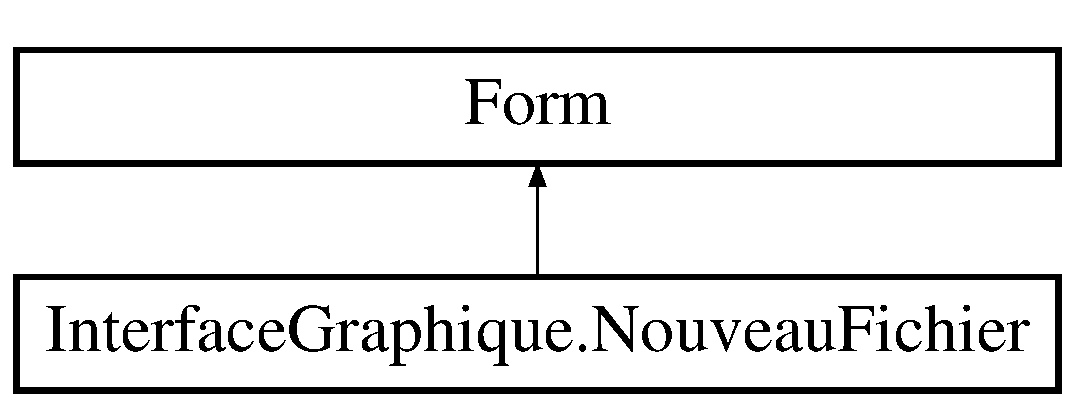
\includegraphics[height=2.000000cm]{class_interface_graphique_1_1_nouveau_fichier}
\end{center}
\end{figure}
\subsection*{Public Member Functions}
\begin{DoxyCompactItemize}
\item 
\hyperlink{class_interface_graphique_1_1_nouveau_fichier_a27efcb30d7aa214fb6d1466fae5806bd}{Nouveau\+Fichier} ()
\end{DoxyCompactItemize}
\subsection*{Public Attributes}
\begin{DoxyCompactItemize}
\item 
string \hyperlink{class_interface_graphique_1_1_nouveau_fichier_a67f78efe104bcc9d7ad7f2a8e105379a}{nom\+Fichier}
\begin{DoxyCompactList}\small\item\em Nom du fichier à créer \end{DoxyCompactList}\end{DoxyCompactItemize}
\subsection*{Protected Member Functions}
\begin{DoxyCompactItemize}
\item 
override void \hyperlink{class_interface_graphique_1_1_nouveau_fichier_a36b20498dae5da1694f04f00ac42dea3}{Dispose} (bool disposing)
\begin{DoxyCompactList}\small\item\em Clean up any resources being used. \end{DoxyCompactList}\end{DoxyCompactItemize}


\subsection{Constructor \& Destructor Documentation}
\index{Interface\+Graphique\+::\+Nouveau\+Fichier@{Interface\+Graphique\+::\+Nouveau\+Fichier}!Nouveau\+Fichier@{Nouveau\+Fichier}}
\index{Nouveau\+Fichier@{Nouveau\+Fichier}!Interface\+Graphique\+::\+Nouveau\+Fichier@{Interface\+Graphique\+::\+Nouveau\+Fichier}}
\subsubsection[{\texorpdfstring{Nouveau\+Fichier()}{NouveauFichier()}}]{\setlength{\rightskip}{0pt plus 5cm}public Interface\+Graphique.\+Nouveau\+Fichier.\+Nouveau\+Fichier (
\begin{DoxyParamCaption}
{}
\end{DoxyParamCaption}
)\hspace{0.3cm}{\ttfamily [inline]}}\hypertarget{class_interface_graphique_1_1_nouveau_fichier_a27efcb30d7aa214fb6d1466fae5806bd}{}\label{class_interface_graphique_1_1_nouveau_fichier_a27efcb30d7aa214fb6d1466fae5806bd}
Constructeur par défaut Initialise les composantes du formulaires.

\begin{DoxyReturn}{Returns}
Aucune 
\end{DoxyReturn}


\subsection{Member Function Documentation}
\index{Interface\+Graphique\+::\+Nouveau\+Fichier@{Interface\+Graphique\+::\+Nouveau\+Fichier}!Dispose@{Dispose}}
\index{Dispose@{Dispose}!Interface\+Graphique\+::\+Nouveau\+Fichier@{Interface\+Graphique\+::\+Nouveau\+Fichier}}
\subsubsection[{\texorpdfstring{Dispose(bool disposing)}{Dispose(bool disposing)}}]{\setlength{\rightskip}{0pt plus 5cm}override void Interface\+Graphique.\+Nouveau\+Fichier.\+Dispose (
\begin{DoxyParamCaption}
\item[{bool}]{disposing}
\end{DoxyParamCaption}
)\hspace{0.3cm}{\ttfamily [inline]}, {\ttfamily [protected]}}\hypertarget{class_interface_graphique_1_1_nouveau_fichier_a36b20498dae5da1694f04f00ac42dea3}{}\label{class_interface_graphique_1_1_nouveau_fichier_a36b20498dae5da1694f04f00ac42dea3}


Clean up any resources being used. 


\begin{DoxyParams}{Parameters}
{\em disposing} & true if managed resources should be disposed; otherwise, false.\\
\hline
\end{DoxyParams}


\subsection{Member Data Documentation}
\index{Interface\+Graphique\+::\+Nouveau\+Fichier@{Interface\+Graphique\+::\+Nouveau\+Fichier}!nom\+Fichier@{nom\+Fichier}}
\index{nom\+Fichier@{nom\+Fichier}!Interface\+Graphique\+::\+Nouveau\+Fichier@{Interface\+Graphique\+::\+Nouveau\+Fichier}}
\subsubsection[{\texorpdfstring{nom\+Fichier}{nomFichier}}]{\setlength{\rightskip}{0pt plus 5cm}string Interface\+Graphique.\+Nouveau\+Fichier.\+nom\+Fichier}\hypertarget{class_interface_graphique_1_1_nouveau_fichier_a67f78efe104bcc9d7ad7f2a8e105379a}{}\label{class_interface_graphique_1_1_nouveau_fichier_a67f78efe104bcc9d7ad7f2a8e105379a}


Nom du fichier à créer 



The documentation for this class was generated from the following files\+:\begin{DoxyCompactItemize}
\item 
Sources/\+Interface\+Graphique/\+Formulaires\+Sys\+Fichiers/\hyperlink{_nouveau_fichier_8cs}{Nouveau\+Fichier.\+cs}\item 
Sources/\+Interface\+Graphique/\+Formulaires\+Sys\+Fichiers/Nouveau\+Fichier.\+Designer.\+cs\end{DoxyCompactItemize}

\hypertarget{class_interface_graphique_1_1_pop_out_interface}{}\section{Interface\+Graphique.\+Pop\+Out\+Interface Class Reference}
\label{class_interface_graphique_1_1_pop_out_interface}\index{Interface\+Graphique.\+Pop\+Out\+Interface@{Interface\+Graphique.\+Pop\+Out\+Interface}}
Inheritance diagram for Interface\+Graphique.\+Pop\+Out\+Interface\+:\begin{figure}[H]
\begin{center}
\leavevmode
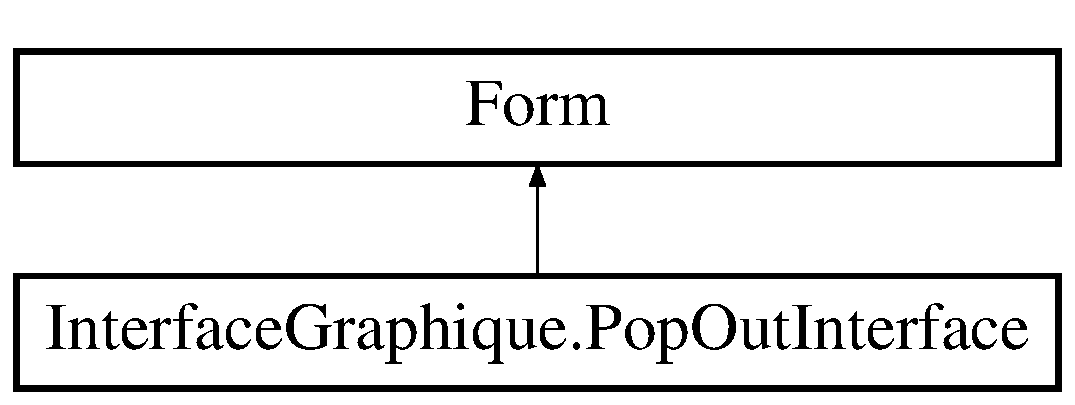
\includegraphics[height=2.000000cm]{class_interface_graphique_1_1_pop_out_interface}
\end{center}
\end{figure}
\subsection*{Public Member Functions}
\begin{DoxyCompactItemize}
\item 
\hyperlink{group__inf2990_gaef377ac8e5964cc5d2dfcdde8a130c99}{Pop\+Out\+Interface} ()
\end{DoxyCompactItemize}
\subsection*{Protected Member Functions}
\begin{DoxyCompactItemize}
\item 
override void \hyperlink{class_interface_graphique_1_1_pop_out_interface_a78c74282aa06c22d461e1d779e8fec89}{Dispose} (bool disposing)
\begin{DoxyCompactList}\small\item\em Clean up any resources being used. \end{DoxyCompactList}\end{DoxyCompactItemize}


\subsection{Member Function Documentation}
\index{Interface\+Graphique\+::\+Pop\+Out\+Interface@{Interface\+Graphique\+::\+Pop\+Out\+Interface}!Dispose@{Dispose}}
\index{Dispose@{Dispose}!Interface\+Graphique\+::\+Pop\+Out\+Interface@{Interface\+Graphique\+::\+Pop\+Out\+Interface}}
\subsubsection[{\texorpdfstring{Dispose(bool disposing)}{Dispose(bool disposing)}}]{\setlength{\rightskip}{0pt plus 5cm}override void Interface\+Graphique.\+Pop\+Out\+Interface.\+Dispose (
\begin{DoxyParamCaption}
\item[{bool}]{disposing}
\end{DoxyParamCaption}
)\hspace{0.3cm}{\ttfamily [inline]}, {\ttfamily [protected]}}\hypertarget{class_interface_graphique_1_1_pop_out_interface_a78c74282aa06c22d461e1d779e8fec89}{}\label{class_interface_graphique_1_1_pop_out_interface_a78c74282aa06c22d461e1d779e8fec89}


Clean up any resources being used. 


\begin{DoxyParams}{Parameters}
{\em disposing} & true if managed resources should be disposed; otherwise, false.\\
\hline
\end{DoxyParams}


The documentation for this class was generated from the following files\+:\begin{DoxyCompactItemize}
\item 
Sources/\+Interface\+Graphique/\hyperlink{_pop_out_interface_8cs}{Pop\+Out\+Interface.\+cs}\item 
Sources/\+Interface\+Graphique/Pop\+Out\+Interface.\+Designer.\+cs\end{DoxyCompactItemize}

\hypertarget{class_usine_abstraite}{}\section{Usine\+Abstraite Class Reference}
\label{class_usine_abstraite}\index{Usine\+Abstraite@{Usine\+Abstraite}}


Classe de base abstraite des usines qui seront utilis�es pour cr�er les diff�rents noeuds de l\textquotesingle{}arbre de rendu.  




{\ttfamily \#include $<$Usine\+Noeud.\+h$>$}

Inheritance diagram for Usine\+Abstraite\+:\begin{figure}[H]
\begin{center}
\leavevmode
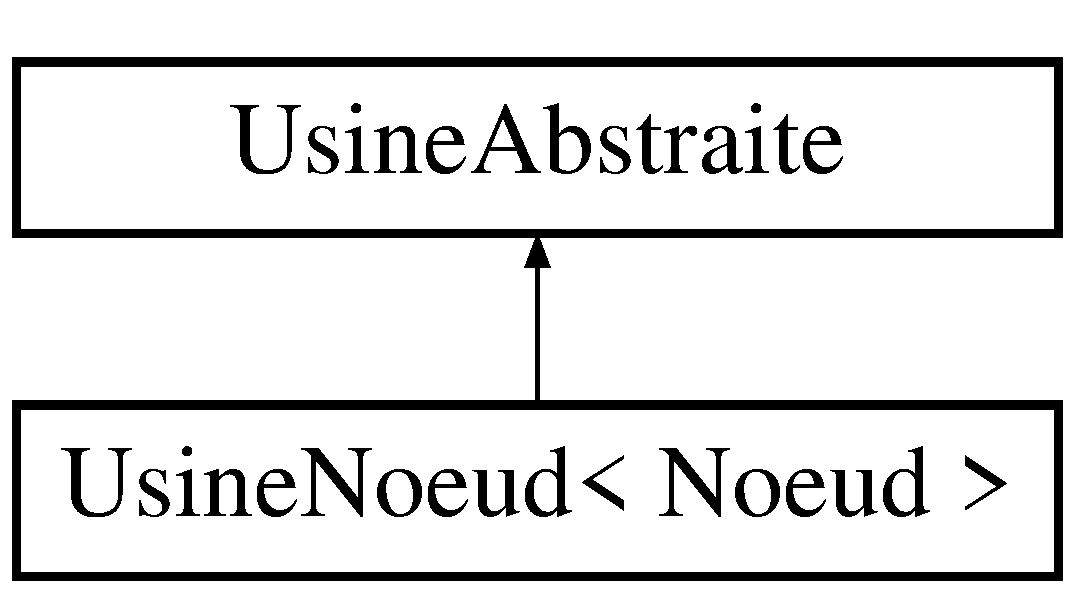
\includegraphics[height=2.000000cm]{class_usine_abstraite}
\end{center}
\end{figure}
\subsection*{Public Member Functions}
\begin{DoxyCompactItemize}
\item 
virtual std\+::shared\+\_\+ptr$<$ \hyperlink{class_noeud_abstrait}{Noeud\+Abstrait} $>$ {\bfseries creer\+Noeud} () const  =0\hypertarget{class_usine_abstraite_aa4eb915fd5c8cc339342181541d85e1f}{}\label{class_usine_abstraite_aa4eb915fd5c8cc339342181541d85e1f}

\end{DoxyCompactItemize}
\subsection*{Protected Member Functions}
\begin{DoxyCompactItemize}
\item 
{\bfseries Usine\+Abstraite} (std\+::string nom)\hypertarget{class_usine_abstraite_a6a5dc32968aa9a7ddd052c2b8f694447}{}\label{class_usine_abstraite_a6a5dc32968aa9a7ddd052c2b8f694447}

\item 
const std\+::string \& \hyperlink{group__inf2990_gad39877ea31a37efc3e58708193155c3c}{obtenir\+Nom} () const 
\begin{DoxyCompactList}\small\item\em Retourne le nom associ� � l\textquotesingle{}usine. \end{DoxyCompactList}\end{DoxyCompactItemize}


\subsection{Detailed Description}
Classe de base abstraite des usines qui seront utilis�es pour cr�er les diff�rents noeuds de l\textquotesingle{}arbre de rendu. 

\begin{DoxyAuthor}{Author}
Martin Bisson 
\end{DoxyAuthor}
\begin{DoxyDate}{Date}
2001-\/01-\/28 
\end{DoxyDate}


The documentation for this class was generated from the following file\+:\begin{DoxyCompactItemize}
\item 
Sources/\+D\+L\+L/\+Arbre/\+Usines/\hyperlink{_usine_noeud_8h}{Usine\+Noeud.\+h}\end{DoxyCompactItemize}

\hypertarget{class_usine_noeud}{}\section{Usine\+Noeud$<$ Noeud $>$ Class Template Reference}
\label{class_usine_noeud}\index{Usine\+Noeud$<$ Noeud $>$@{Usine\+Noeud$<$ Noeud $>$}}


Class template permettant de cr�er un type de noeud concret pour l\textquotesingle{}arbre de rendu.  




{\ttfamily \#include $<$Usine\+Noeud.\+h$>$}

Inheritance diagram for Usine\+Noeud$<$ Noeud $>$\+:\begin{figure}[H]
\begin{center}
\leavevmode
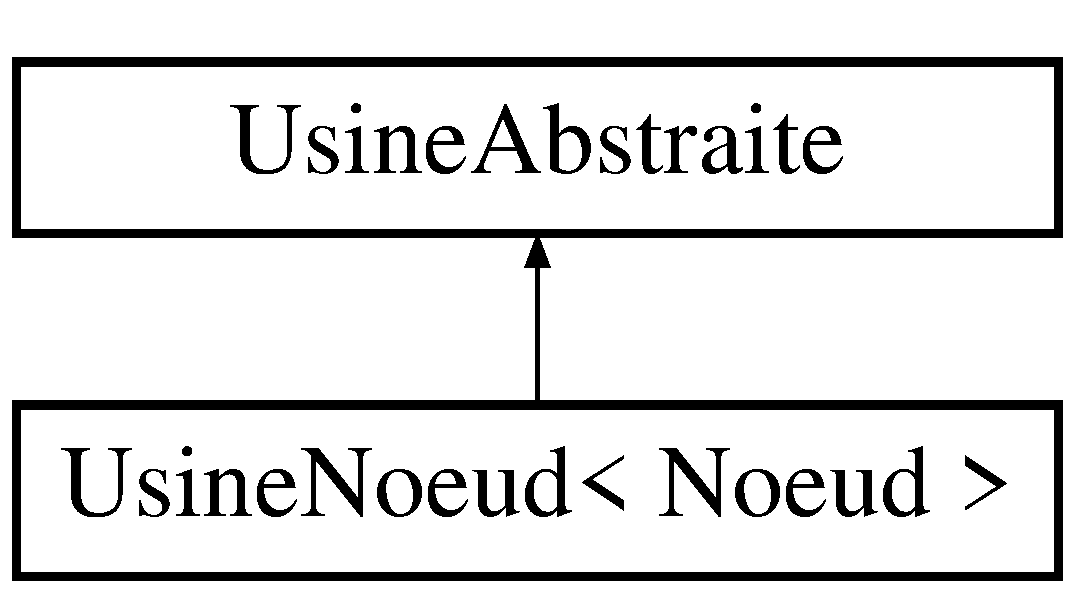
\includegraphics[height=2.000000cm]{class_usine_noeud}
\end{center}
\end{figure}
\subsection*{Public Member Functions}
\begin{DoxyCompactItemize}
\item 
\hyperlink{class_usine_noeud_ad09d79d36fb0135b51224484ca0f47f0}{$\sim$\+Usine\+Noeud} ()\hypertarget{class_usine_noeud_ad09d79d36fb0135b51224484ca0f47f0}{}\label{class_usine_noeud_ad09d79d36fb0135b51224484ca0f47f0}

\begin{DoxyCompactList}\small\item\em Destructeur vide d�clar� virtuel pour les classes d�riv�es. \end{DoxyCompactList}\item 
virtual std\+::shared\+\_\+ptr$<$ \hyperlink{class_noeud_abstrait}{Noeud\+Abstrait} $>$ \hyperlink{group__inf2990_ga4f07b0dc2254e418808b783f4555e693}{creer\+Noeud} () const  override
\begin{DoxyCompactList}\small\item\em Fonction � surcharger pour la cr�ation d\textquotesingle{}un noeud. \end{DoxyCompactList}\item 
\hyperlink{class_usine_noeud_a14ce73da1a318f53746607658837c56a}{Usine\+Noeud} (const std\+::string \&nom\+Usine, const std\+::string \&nom\+Modele)\hypertarget{class_usine_noeud_a14ce73da1a318f53746607658837c56a}{}\label{class_usine_noeud_a14ce73da1a318f53746607658837c56a}

\begin{DoxyCompactList}\small\item\em Constructeur qui prend le nom associ� � l\textquotesingle{}usine. \end{DoxyCompactList}\end{DoxyCompactItemize}
\subsection*{Protected Attributes}
\begin{DoxyCompactItemize}
\item 
modele\+::\+Modele3D \hyperlink{class_usine_noeud_a41150bf720451994fc944328e5966de7}{modele\+\_\+}\hypertarget{class_usine_noeud_a41150bf720451994fc944328e5966de7}{}\label{class_usine_noeud_a41150bf720451994fc944328e5966de7}

\begin{DoxyCompactList}\small\item\em Mod�le 3D correspondant � ce noeud. \end{DoxyCompactList}\item 
opengl\+::\+V\+BO \hyperlink{class_usine_noeud_a255ba23be7c197be82afdd3e7de6a651}{vbo\+\_\+}\hypertarget{class_usine_noeud_a255ba23be7c197be82afdd3e7de6a651}{}\label{class_usine_noeud_a255ba23be7c197be82afdd3e7de6a651}

\begin{DoxyCompactList}\small\item\em Storage pour le dessin du mod�le. \end{DoxyCompactList}\end{DoxyCompactItemize}
\subsection*{Additional Inherited Members}


\subsection{Detailed Description}
\subsubsection*{template$<$typename Noeud$>$\\*
class Usine\+Noeud$<$ Noeud $>$}

Class template permettant de cr�er un type de noeud concret pour l\textquotesingle{}arbre de rendu. 

\begin{DoxyAuthor}{Author}
Martin Paradis 
\end{DoxyAuthor}
\begin{DoxyDate}{Date}
2015-\/06-\/24 
\end{DoxyDate}


The documentation for this class was generated from the following file\+:\begin{DoxyCompactItemize}
\item 
Sources/\+D\+L\+L/\+Arbre/\+Usines/\hyperlink{_usine_noeud_8h}{Usine\+Noeud.\+h}\end{DoxyCompactItemize}

\hypertarget{class_visiteur_abstrait}{}\section{Visiteur\+Abstrait Class Reference}
\label{class_visiteur_abstrait}\index{Visiteur\+Abstrait@{Visiteur\+Abstrait}}


Classe de base du patron visiteur utilis�e pour effectuer des manipulations sur l\textquotesingle{}arbre de rendu.  




{\ttfamily \#include $<$Visiteur\+Abstrait.\+h$>$}

Inheritance diagram for Visiteur\+Abstrait\+:\begin{figure}[H]
\begin{center}
\leavevmode
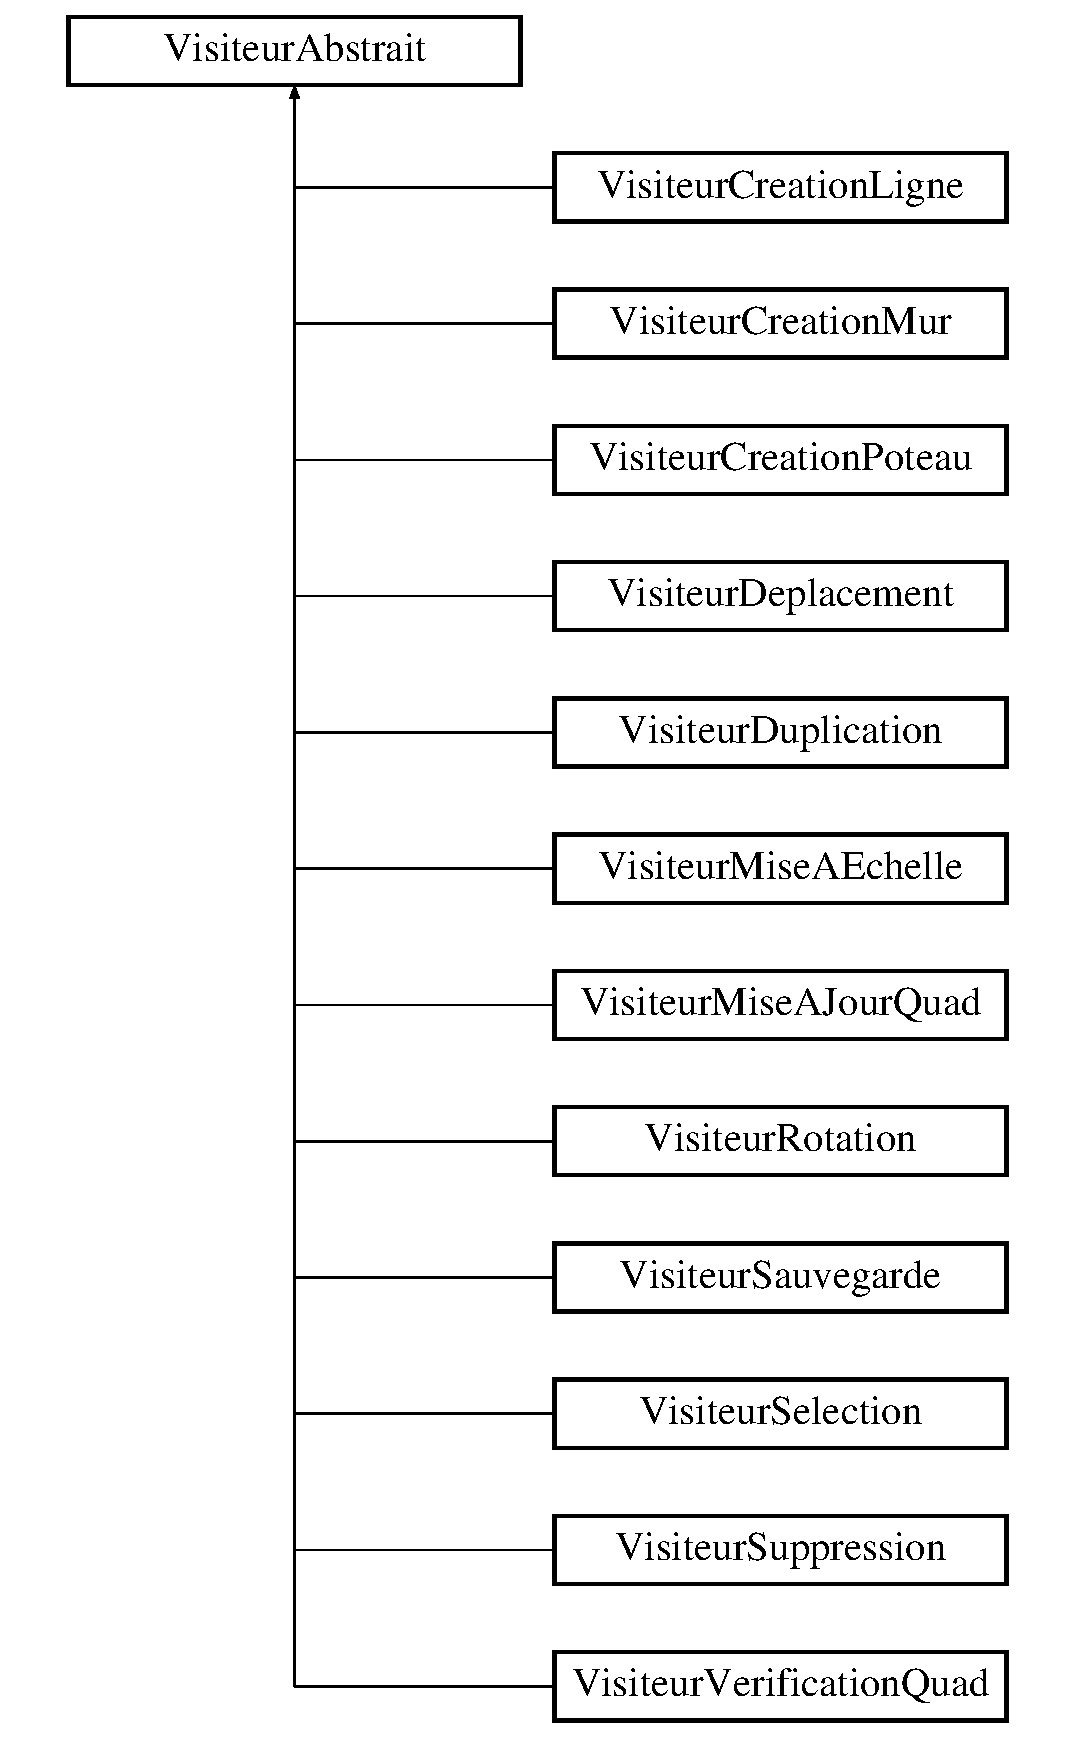
\includegraphics[height=12.000000cm]{class_visiteur_abstrait}
\end{center}
\end{figure}
\subsection*{Public Member Functions}
\begin{DoxyCompactItemize}
\item 
\hyperlink{group__inf2990_gab30d8c699bab1b4538f79e5750468d2d}{Visiteur\+Abstrait} ()
\begin{DoxyCompactList}\small\item\em Constructeur par d�faut. \end{DoxyCompactList}\item 
virtual \hyperlink{group__inf2990_ga49b82dbd9c247719aece829132013f45}{$\sim$\+Visiteur\+Abstrait} ()
\begin{DoxyCompactList}\small\item\em Destructeur. \end{DoxyCompactList}\item 
void \hyperlink{group__inf2990_ga865f6a23e40671d242c4b1be08e5b64a}{assigner\+Position\+Relative} (glm\+::dvec3 position\+Relative)
\item 
void \hyperlink{group__inf2990_ga502ec76a196806a076cfb94922880361}{assigner\+Position\+Relative\+Avant} (glm\+::dvec3 position\+Relative\+Avant)
\item 
void \hyperlink{group__inf2990_ga584c5fd6e43fa50348f915645aa7106f}{assigner\+Position\+Relative\+Apres} (glm\+::dvec3 position\+Relative\+Apres)
\item 
void \hyperlink{group__inf2990_ga3036c649ed93909baf0060a3055e3d83}{assigner\+Angle\+Rotation} (double angle\+Rotation)
\item 
void \hyperlink{group__inf2990_gaeb5a06db4d8895f86b8d6563974461c4}{assigner\+Facteur\+Mise\+A\+Echelle} (double facteur\+Dimension)
\item 
void \hyperlink{group__inf2990_gac9697e56d1de349151d72e6030db45b9}{assigner\+Est\+Affiche} (const bool \&est\+Affiche)
\item 
void \hyperlink{group__inf2990_ga5a9d4c82f2fe5ae47f13754cd2587c4d}{assigner\+Est\+Drag} (const bool \&est\+Drag)
\item 
\hyperlink{class_noeud_abstrait}{Noeud\+Abstrait} $\ast$ \hyperlink{group__inf2990_gaeb7b5cd0cad75b1ab4caa2f8a65d5fba}{obtenir\+Reference\+Noeud} ()
\item 
bool \hyperlink{group__inf2990_gad841f0b531514e5ffa98b591dc19004a}{obtenir\+Est\+Drag} ()
\item 
virtual void \hyperlink{group__inf2990_gace1e0b18f5e6a01d16c7ed2d55fffbe3}{visiter} (\hyperlink{class_arbre_rendu}{Arbre\+Rendu} $\ast$noeud)
\item 
virtual void \hyperlink{group__inf2990_ga06d7edfabeb6e0bcc7451128bed6edba}{visiter} (\hyperlink{class_noeud_table}{Noeud\+Table} $\ast$noeud)
\item 
virtual void \hyperlink{group__inf2990_ga46caa33e562f0f200c247562606ca63a}{visiter} (\hyperlink{class_noeud_poteau}{Noeud\+Poteau} $\ast$noeud)
\item 
virtual void \hyperlink{group__inf2990_gaca7d5269422bb4564b03f6a73a381b8e}{visiter} (\hyperlink{class_noeud_mur}{Noeud\+Mur} $\ast$noeud)
\item 
virtual void \hyperlink{group__inf2990_ga3bc8e290c245c5c2e6df6b0669d9e72d}{visiter} (\hyperlink{class_noeud_ligne}{Noeud\+Ligne} $\ast$noeud)
\item 
virtual void \hyperlink{group__inf2990_ga73238504ddd7c749f407899c1660ea1d}{visiter} (\hyperlink{class_noeud_segment}{Noeud\+Segment} $\ast$noeud)
\item 
virtual void \hyperlink{group__inf2990_gafcb35663383811eaca17cf5155c0b03d}{visiter} (\hyperlink{class_noeud_duplication}{Noeud\+Duplication} $\ast$noeud)
\item 
virtual void \hyperlink{group__inf2990_ga17b03f5673cb67859cb6ba724fef9190}{visiter} (\hyperlink{class_noeud_depart}{Noeud\+Depart} $\ast$noeud)
\item 
virtual void \hyperlink{group__inf2990_gadada2d404915273990ff60d03e5857b0}{visiter} (\hyperlink{class_noeud_jonction}{Noeud\+Jonction} $\ast$noeud)
\item 
virtual void {\bfseries visiter} (\hyperlink{class_noeud_robot}{Noeud\+Robot} $\ast$noeud)
\end{DoxyCompactItemize}
\subsection*{Protected Attributes}
\begin{DoxyCompactItemize}
\item 
glm\+::dvec3 {\bfseries position\+Relative\+\_\+} \{ glm\+::dvec3() \}\hypertarget{class_visiteur_abstrait_a56f8d1abe8a3cc316cdcfdb3730e9d5f}{}\label{class_visiteur_abstrait_a56f8d1abe8a3cc316cdcfdb3730e9d5f}

\item 
glm\+::dvec3 {\bfseries position\+Relative\+Avant\+\_\+} \{ glm\+::dvec3() \}\hypertarget{class_visiteur_abstrait_acfad330cb989c5baef39aa59a6013a81}{}\label{class_visiteur_abstrait_acfad330cb989c5baef39aa59a6013a81}

\item 
glm\+::dvec3 {\bfseries position\+Relative\+Apres\+\_\+} \{ glm\+::dvec3() \}\hypertarget{class_visiteur_abstrait_a55cec3f2baeee84bed64948c9ed94b75}{}\label{class_visiteur_abstrait_a55cec3f2baeee84bed64948c9ed94b75}

\item 
bool {\bfseries est\+Drag\+\_\+} \{ false \}\hypertarget{class_visiteur_abstrait_abaa36bdb41ac9f9932c7a4d1ccbe9774}{}\label{class_visiteur_abstrait_abaa36bdb41ac9f9932c7a4d1ccbe9774}

\item 
double {\bfseries angle\+Rotation\+\_\+} \{ 0.\+0 \}\hypertarget{class_visiteur_abstrait_a534b6a86b0f91dd604b47c4d00a47ac9}{}\label{class_visiteur_abstrait_a534b6a86b0f91dd604b47c4d00a47ac9}

\item 
double {\bfseries facteur\+Mise\+A\+Echelle\+\_\+} \{ 0.\+0 \}\hypertarget{class_visiteur_abstrait_a8eade6c59a550a5cbb9b68b2cc8ec0b0}{}\label{class_visiteur_abstrait_a8eade6c59a550a5cbb9b68b2cc8ec0b0}

\item 
bool {\bfseries est\+Affiche\+\_\+} \{ false \}\hypertarget{class_visiteur_abstrait_a1c0c63b97e92c80396086386200b2081}{}\label{class_visiteur_abstrait_a1c0c63b97e92c80396086386200b2081}

\item 
\hyperlink{class_noeud_abstrait}{Noeud\+Abstrait} $\ast$ {\bfseries reference\+Noeud\+\_\+} \{ nullptr \}\hypertarget{class_visiteur_abstrait_a3c79044bbcffb9db9ec8412d3142c2b7}{}\label{class_visiteur_abstrait_a3c79044bbcffb9db9ec8412d3142c2b7}

\end{DoxyCompactItemize}


\subsection{Detailed Description}
Classe de base du patron visiteur utilis�e pour effectuer des manipulations sur l\textquotesingle{}arbre de rendu. 

Cette classe abstraite comprend l\textquotesingle{}interface de base que doivent implanter tous les visiteurs concrets.

\begin{DoxyAuthor}{Author}
Olivier St-\/\+Amour 
\end{DoxyAuthor}
\begin{DoxyDate}{Date}
2016-\/01-\/13 
\end{DoxyDate}


The documentation for this class was generated from the following files\+:\begin{DoxyCompactItemize}
\item 
Sources/\+D\+L\+L/\+Visiteur/\hyperlink{_visiteur_abstrait_8h}{Visiteur\+Abstrait.\+h}\item 
Sources/\+D\+L\+L/\+Visiteur/Visteur\+Abstrait.\+cpp\end{DoxyCompactItemize}

\hypertarget{class_visiteur_creation_ligne}{}\section{Visiteur\+Creation\+Ligne Class Reference}
\label{class_visiteur_creation_ligne}\index{Visiteur\+Creation\+Ligne@{Visiteur\+Creation\+Ligne}}


Visiteur permettant d\textquotesingle{}initialiser la cr�ation d\textquotesingle{}une ligne.  




{\ttfamily \#include $<$Visiteur\+Creation\+Ligne.\+h$>$}

Inheritance diagram for Visiteur\+Creation\+Ligne\+:\begin{figure}[H]
\begin{center}
\leavevmode
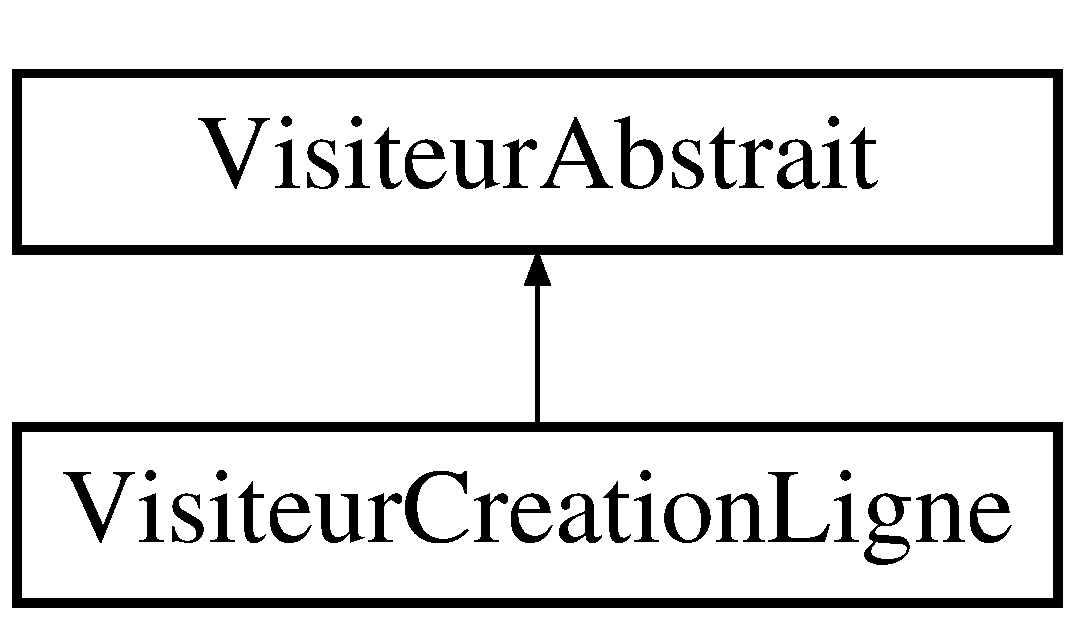
\includegraphics[height=2.000000cm]{class_visiteur_creation_ligne}
\end{center}
\end{figure}
\subsection*{Public Member Functions}
\begin{DoxyCompactItemize}
\item 
\hyperlink{group__inf2990_ga0ba68a03489b929c1505fab9144024de}{Visiteur\+Creation\+Ligne} ()
\begin{DoxyCompactList}\small\item\em Constructeur par d�faut. \end{DoxyCompactList}\item 
virtual \hyperlink{group__inf2990_ga3c519a1b589bace4bbf43128111415f0}{$\sim$\+Visiteur\+Creation\+Ligne} ()
\begin{DoxyCompactList}\small\item\em Destructeur. \end{DoxyCompactList}\item 
virtual void \hyperlink{group__inf2990_gaf291427ae3c4bf5cf03eac2a3be1a4f4}{visiter} (\hyperlink{class_arbre_rendu}{Arbre\+Rendu} $\ast$noeud)
\begin{DoxyCompactList}\small\item\em Creation de poteau sur l\textquotesingle{}arbre de rendu. \end{DoxyCompactList}\item 
virtual void \hyperlink{group__inf2990_ga6e9da333f12cc44e62acabc896754b39}{visiter} (\hyperlink{class_noeud_table}{Noeud\+Table} $\ast$noeud)
\begin{DoxyCompactList}\small\item\em Creation de poteau sur la table. \end{DoxyCompactList}\end{DoxyCompactItemize}
\subsection*{Additional Inherited Members}


\subsection{Detailed Description}
Visiteur permettant d\textquotesingle{}initialiser la cr�ation d\textquotesingle{}une ligne. 

\begin{DoxyAuthor}{Author}
Olivier St-\/\+Amour 
\end{DoxyAuthor}
\begin{DoxyDate}{Date}
2016-\/02-\/15 
\end{DoxyDate}


The documentation for this class was generated from the following files\+:\begin{DoxyCompactItemize}
\item 
Sources/\+D\+L\+L/\+Visiteur/\hyperlink{_visiteur_creation_ligne_8h}{Visiteur\+Creation\+Ligne.\+h}\item 
Sources/\+D\+L\+L/\+Visiteur/\hyperlink{_visiteur_creation_ligne_8cpp}{Visiteur\+Creation\+Ligne.\+cpp}\item 
Sources/\+D\+L\+L/\+Visiteur/\hyperlink{_visiteur_creation_mur_8cpp}{Visiteur\+Creation\+Mur.\+cpp}\end{DoxyCompactItemize}

\hypertarget{class_visiteur_creation_mur}{}\section{Visiteur\+Creation\+Mur Class Reference}
\label{class_visiteur_creation_mur}\index{Visiteur\+Creation\+Mur@{Visiteur\+Creation\+Mur}}


Visiteur permettant d\textquotesingle{}initialiser la cr�ation d\textquotesingle{}un mur.  




{\ttfamily \#include $<$Visiteur\+Creation\+Mur.\+h$>$}

Inheritance diagram for Visiteur\+Creation\+Mur\+:\begin{figure}[H]
\begin{center}
\leavevmode
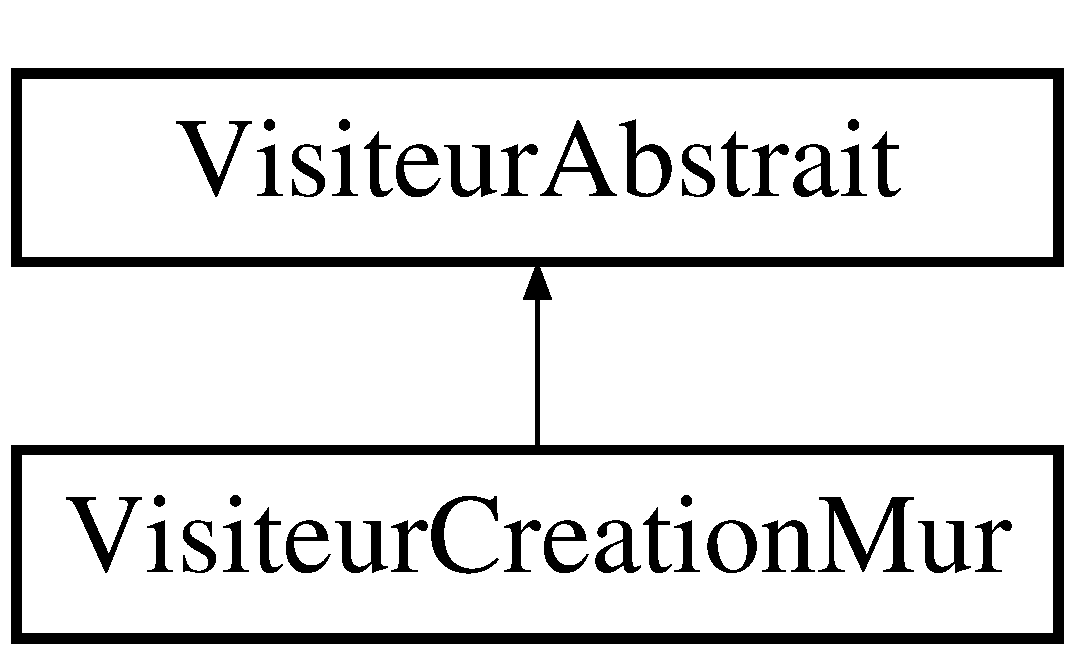
\includegraphics[height=2.000000cm]{class_visiteur_creation_mur}
\end{center}
\end{figure}
\subsection*{Public Member Functions}
\begin{DoxyCompactItemize}
\item 
\hyperlink{group__inf2990_ga35478ac71c635e34f309a8a3cf3e0d4d}{Visiteur\+Creation\+Mur} ()
\begin{DoxyCompactList}\small\item\em Constructeur par d�faut. \end{DoxyCompactList}\item 
virtual \hyperlink{group__inf2990_ga1bf64b5cd1a6ecdefa83699cde287969}{$\sim$\+Visiteur\+Creation\+Mur} ()
\begin{DoxyCompactList}\small\item\em Destructeur. \end{DoxyCompactList}\item 
virtual void \hyperlink{group__inf2990_ga37d32718c10ffe24225627001ea6ad6f}{visiter} (\hyperlink{class_arbre_rendu}{Arbre\+Rendu} $\ast$noeud)
\begin{DoxyCompactList}\small\item\em Creation de poteau sur l\textquotesingle{}arbre de rendu. \end{DoxyCompactList}\item 
virtual void \hyperlink{group__inf2990_ga833ec993cf27bff664cb6ac938c73bec}{visiter} (\hyperlink{class_noeud_table}{Noeud\+Table} $\ast$noeud)
\begin{DoxyCompactList}\small\item\em Creation de poteau sur la table. \end{DoxyCompactList}\end{DoxyCompactItemize}
\subsection*{Additional Inherited Members}


\subsection{Detailed Description}
Visiteur permettant d\textquotesingle{}initialiser la cr�ation d\textquotesingle{}un mur. 

\begin{DoxyAuthor}{Author}
Olivier St-\/\+Amour 
\end{DoxyAuthor}
\begin{DoxyDate}{Date}
2016-\/02-\/15 
\end{DoxyDate}


The documentation for this class was generated from the following files\+:\begin{DoxyCompactItemize}
\item 
Sources/\+D\+L\+L/\+Visiteur/\hyperlink{_visiteur_creation_mur_8h}{Visiteur\+Creation\+Mur.\+h}\item 
Sources/\+D\+L\+L/\+Visiteur/\hyperlink{_visiteur_creation_mur_8cpp}{Visiteur\+Creation\+Mur.\+cpp}\end{DoxyCompactItemize}

\hypertarget{class_visiteur_creation_poteau}{}\section{Visiteur\+Creation\+Poteau Class Reference}
\label{class_visiteur_creation_poteau}\index{Visiteur\+Creation\+Poteau@{Visiteur\+Creation\+Poteau}}


Visiteur permettant d\textquotesingle{}initialiser la cr�ation d\textquotesingle{}un poteau.  




{\ttfamily \#include $<$Visiteur\+Creation\+Poteau.\+h$>$}

Inheritance diagram for Visiteur\+Creation\+Poteau\+:\begin{figure}[H]
\begin{center}
\leavevmode
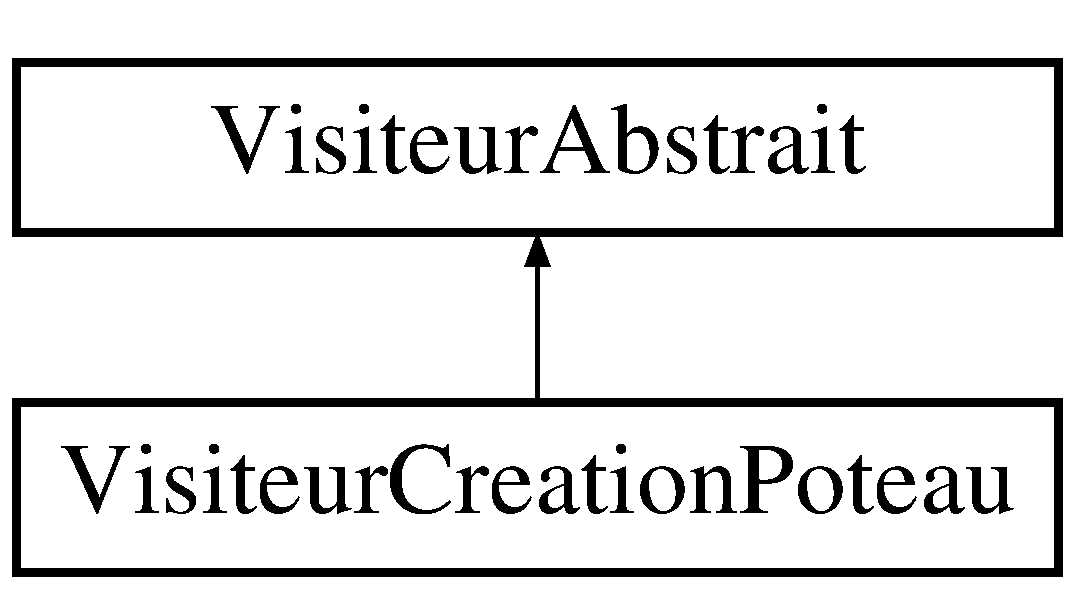
\includegraphics[height=2.000000cm]{class_visiteur_creation_poteau}
\end{center}
\end{figure}
\subsection*{Public Member Functions}
\begin{DoxyCompactItemize}
\item 
\hyperlink{group__inf2990_gaa1ee1f935b8aa91df1ac2a140056f61a}{Visiteur\+Creation\+Poteau} ()
\begin{DoxyCompactList}\small\item\em Constructeur par d�faut. \end{DoxyCompactList}\item 
virtual \hyperlink{group__inf2990_ga7384d51cae9e14fffc2a89d893373b42}{$\sim$\+Visiteur\+Creation\+Poteau} ()
\begin{DoxyCompactList}\small\item\em Destructeur. \end{DoxyCompactList}\item 
virtual void \hyperlink{group__inf2990_gaf0279741c32ebef02a30d3c293f83301}{visiter} (\hyperlink{class_arbre_rendu}{Arbre\+Rendu} $\ast$noeud)
\begin{DoxyCompactList}\small\item\em Creation de poteau sur l\textquotesingle{}arbre de rendu. \end{DoxyCompactList}\item 
virtual void \hyperlink{group__inf2990_gaac0e9943fddd99dce301f16fc54696aa}{visiter} (\hyperlink{class_noeud_table}{Noeud\+Table} $\ast$noeud)
\begin{DoxyCompactList}\small\item\em Creation de poteau sur la table. \end{DoxyCompactList}\end{DoxyCompactItemize}
\subsection*{Additional Inherited Members}


\subsection{Detailed Description}
Visiteur permettant d\textquotesingle{}initialiser la cr�ation d\textquotesingle{}un poteau. 

\begin{DoxyAuthor}{Author}
Fr�d�ric Gr�goire 
\end{DoxyAuthor}
\begin{DoxyDate}{Date}
2016-\/02-\/15 
\end{DoxyDate}


The documentation for this class was generated from the following files\+:\begin{DoxyCompactItemize}
\item 
Sources/\+D\+L\+L/\+Visiteur/\hyperlink{_visiteur_creation_poteau_8h}{Visiteur\+Creation\+Poteau.\+h}\item 
Sources/\+D\+L\+L/\+Visiteur/\hyperlink{_visiteur_creation_poteau_8cpp}{Visiteur\+Creation\+Poteau.\+cpp}\end{DoxyCompactItemize}

\hypertarget{class_visiteur_deplacement}{}\section{Visiteur\+Deplacement Class Reference}
\label{class_visiteur_deplacement}\index{Visiteur\+Deplacement@{Visiteur\+Deplacement}}


Visiteur permettant d\textquotesingle{}effectuer le d�placement d\textquotesingle{}un objet.  




{\ttfamily \#include $<$Visiteur\+Deplacement.\+h$>$}

Inheritance diagram for Visiteur\+Deplacement\+:\begin{figure}[H]
\begin{center}
\leavevmode
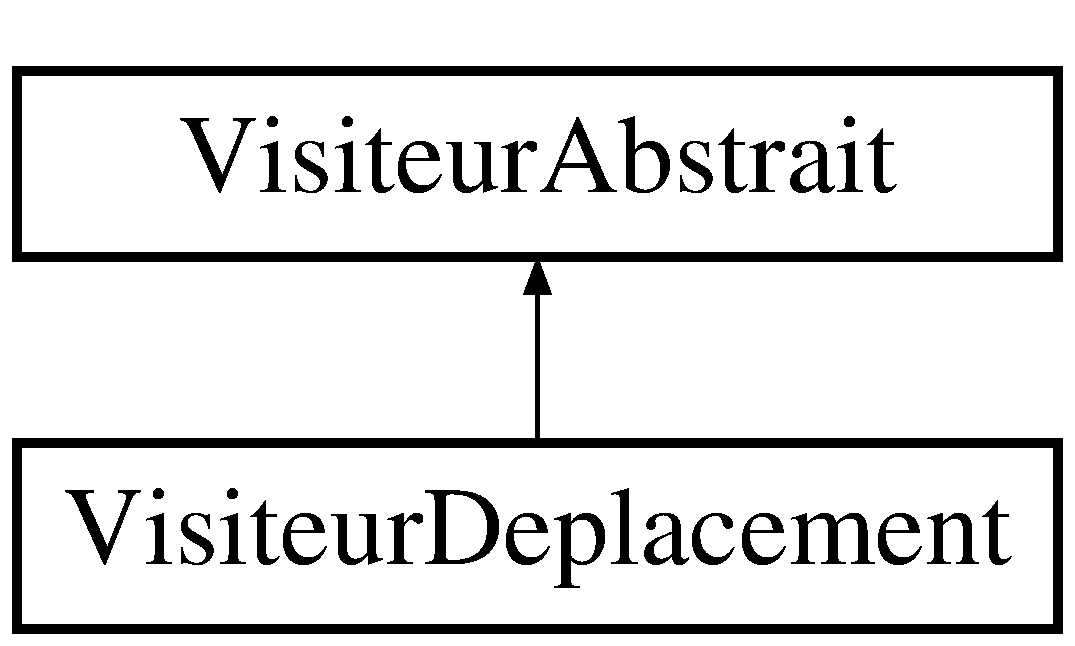
\includegraphics[height=2.000000cm]{class_visiteur_deplacement}
\end{center}
\end{figure}
\subsection*{Public Member Functions}
\begin{DoxyCompactItemize}
\item 
\hyperlink{group__inf2990_ga96164e1d4e72549c09424358e8f01e78}{Visiteur\+Deplacement} ()
\begin{DoxyCompactList}\small\item\em Constructeur par d�faut. \end{DoxyCompactList}\item 
virtual \hyperlink{group__inf2990_ga0f03274d6afe77a7a57f3b7f20417ec8}{$\sim$\+Visiteur\+Deplacement} ()
\begin{DoxyCompactList}\small\item\em Destructeur. \end{DoxyCompactList}\item 
virtual void \hyperlink{group__inf2990_gaf2e0cafbcb1bb7f2adca184c8ace5f51}{visiter} (\hyperlink{class_arbre_rendu}{Arbre\+Rendu} $\ast$noeud)
\item 
virtual void \hyperlink{group__inf2990_ga9599fc0f1de752c95febe9315eefc808}{visiter} (\hyperlink{class_noeud_table}{Noeud\+Table} $\ast$noeud)
\end{DoxyCompactItemize}
\subsection*{Additional Inherited Members}


\subsection{Detailed Description}
Visiteur permettant d\textquotesingle{}effectuer le d�placement d\textquotesingle{}un objet. 

\begin{DoxyAuthor}{Author}
Fr�d�ric Gr�goire 
\end{DoxyAuthor}
\begin{DoxyDate}{Date}
2016-\/02-\/15 
\end{DoxyDate}


The documentation for this class was generated from the following files\+:\begin{DoxyCompactItemize}
\item 
Sources/\+D\+L\+L/\+Visiteur/\hyperlink{_visiteur_deplacement_8h}{Visiteur\+Deplacement.\+h}\item 
Sources/\+D\+L\+L/\+Visiteur/\hyperlink{_visiteur_deplacement_8cpp}{Visiteur\+Deplacement.\+cpp}\end{DoxyCompactItemize}

\hypertarget{class_visiteur_duplication}{}\section{Visiteur\+Duplication Class Reference}
\label{class_visiteur_duplication}\index{Visiteur\+Duplication@{Visiteur\+Duplication}}


Visiteur permettant d\textquotesingle{}effectuer une duplication d\textquotesingle{}un objet.  




{\ttfamily \#include $<$Visiteur\+Duplication.\+h$>$}

Inheritance diagram for Visiteur\+Duplication\+:\begin{figure}[H]
\begin{center}
\leavevmode
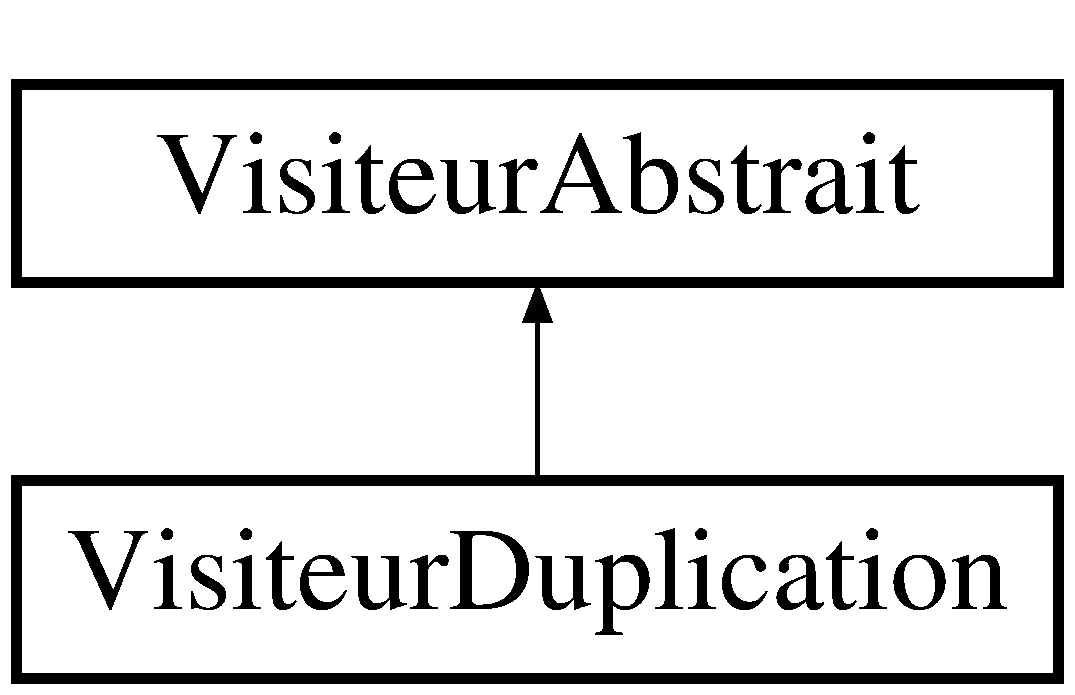
\includegraphics[height=2.000000cm]{class_visiteur_duplication}
\end{center}
\end{figure}
\subsection*{Public Member Functions}
\begin{DoxyCompactItemize}
\item 
\hyperlink{group__inf2990_gacc8fff54253eb394c7ade415f59d57e0}{Visiteur\+Duplication} ()
\begin{DoxyCompactList}\small\item\em Constructeur par d�faut. \end{DoxyCompactList}\item 
virtual \hyperlink{group__inf2990_gab48c0bd69fe4738d85ec48bfe1ae51ea}{$\sim$\+Visiteur\+Duplication} ()
\begin{DoxyCompactList}\small\item\em Destructeur. \end{DoxyCompactList}\item 
void \hyperlink{group__inf2990_gaf2bb1548264e776bc02db31de45c2600}{assigner\+En\+Duplication} (bool en\+Duplication)
\item 
\hyperlink{class_noeud_abstrait}{Noeud\+Abstrait} $\ast$ \hyperlink{group__inf2990_ga4ed636aaf669cf58fb79388882d8aeb4}{obtenir\+Duplication} ()
\item 
virtual void \hyperlink{group__inf2990_gae460a39753df69d448068ead63b3ea44}{visiter} (\hyperlink{class_arbre_rendu}{Arbre\+Rendu} $\ast$noeud)
\item 
virtual void \hyperlink{group__inf2990_ga95037fcce77b99689656f00ad2b7c20d}{visiter} (\hyperlink{class_noeud_table}{Noeud\+Table} $\ast$noeud)
\item 
virtual void \hyperlink{group__inf2990_gaab2dc8ae6ddb353e051ce495f367c6ec}{visiter} (\hyperlink{class_noeud_poteau}{Noeud\+Poteau} $\ast$noeud)
\item 
virtual void \hyperlink{group__inf2990_ga6d17b582e1986d8531c63dc32abeffb0}{visiter} (\hyperlink{class_noeud_mur}{Noeud\+Mur} $\ast$noeud)
\item 
virtual void \hyperlink{group__inf2990_ga239887cb08496e941b67840092d1b98f}{visiter} (\hyperlink{class_noeud_ligne}{Noeud\+Ligne} $\ast$noeud)
\item 
virtual void \hyperlink{group__inf2990_ga41ef8cc862220019224bd00acb63445f}{visiter} (\hyperlink{class_noeud_segment}{Noeud\+Segment} $\ast$noeud)
\item 
virtual void \hyperlink{group__inf2990_ga15bf782d0d5ee9387259d89527fa0049}{visiter} (\hyperlink{class_noeud_jonction}{Noeud\+Jonction} $\ast$noeud)
\item 
virtual void \hyperlink{group__inf2990_gaf586c532b6ce0762b5bd93bb525f01e1}{visiter} (\hyperlink{class_noeud_duplication}{Noeud\+Duplication} $\ast$noeud)
\end{DoxyCompactItemize}
\subsection*{Additional Inherited Members}


\subsection{Detailed Description}
Visiteur permettant d\textquotesingle{}effectuer une duplication d\textquotesingle{}un objet. 

\begin{DoxyAuthor}{Author}
Fr�d�ric Gr�goire 
\end{DoxyAuthor}
\begin{DoxyDate}{Date}
2016-\/02-\/15 
\end{DoxyDate}


The documentation for this class was generated from the following files\+:\begin{DoxyCompactItemize}
\item 
Sources/\+D\+L\+L/\+Visiteur/\hyperlink{_visiteur_duplication_8h}{Visiteur\+Duplication.\+h}\item 
Sources/\+D\+L\+L/\+Visiteur/\hyperlink{_visiteur_duplication_8cpp}{Visiteur\+Duplication.\+cpp}\end{DoxyCompactItemize}

\hypertarget{class_visiteur_mise_a_echelle}{}\section{Visiteur\+Mise\+A\+Echelle Class Reference}
\label{class_visiteur_mise_a_echelle}\index{Visiteur\+Mise\+A\+Echelle@{Visiteur\+Mise\+A\+Echelle}}


Visiteur permettant d\textquotesingle{}effectuer une mise � �chelle d\textquotesingle{}un objet.  




{\ttfamily \#include $<$Visiteur\+Mise\+A\+Echelle.\+h$>$}

Inheritance diagram for Visiteur\+Mise\+A\+Echelle\+:\begin{figure}[H]
\begin{center}
\leavevmode
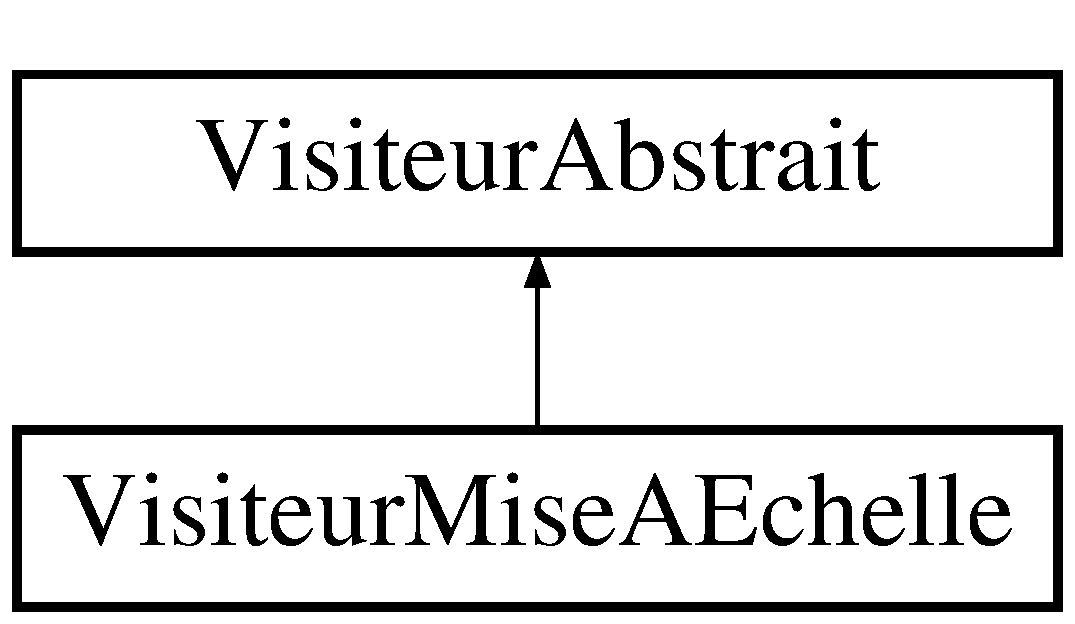
\includegraphics[height=2.000000cm]{class_visiteur_mise_a_echelle}
\end{center}
\end{figure}
\subsection*{Public Member Functions}
\begin{DoxyCompactItemize}
\item 
\hyperlink{group__inf2990_ga252454ee6cfebb8eccc7d03368dc3975}{Visiteur\+Mise\+A\+Echelle} ()
\begin{DoxyCompactList}\small\item\em Constructeur par d�faut. \end{DoxyCompactList}\item 
virtual \hyperlink{group__inf2990_gae0e9751c85dffadd24a92525a72ca8cf}{$\sim$\+Visiteur\+Mise\+A\+Echelle} ()
\begin{DoxyCompactList}\small\item\em Destructeur. \end{DoxyCompactList}\item 
void \hyperlink{group__inf2990_ga10bd3598073b82cb9cac5b1ec275f555}{initialiser} (\hyperlink{class_arbre_rendu}{Arbre\+Rendu} $\ast$arbre)
\item 
void \hyperlink{group__inf2990_ga29fa62f8ff04624a6b6d5626a683511c}{reinitialiser} (\hyperlink{class_arbre_rendu}{Arbre\+Rendu} $\ast$arbre)
\item 
virtual void \hyperlink{group__inf2990_ga983f4e5850c07931015fd022946896ea}{visiter} (\hyperlink{class_arbre_rendu}{Arbre\+Rendu} $\ast$noeud)
\item 
virtual void \hyperlink{group__inf2990_ga81064ba6106c20ab9a554b017525b264}{visiter} (\hyperlink{class_noeud_table}{Noeud\+Table} $\ast$noeud)
\item 
virtual void \hyperlink{group__inf2990_gae56df11d127d8cd13e2a4d805d419c45}{visiter} (\hyperlink{class_noeud_poteau}{Noeud\+Poteau} $\ast$noeud)
\item 
virtual void \hyperlink{group__inf2990_ga2a7721dd07512c79d156534beddead02}{visiter} (\hyperlink{class_noeud_mur}{Noeud\+Mur} $\ast$noeud)
\end{DoxyCompactItemize}
\subsection*{Additional Inherited Members}


\subsection{Detailed Description}
Visiteur permettant d\textquotesingle{}effectuer une mise � �chelle d\textquotesingle{}un objet. 

\begin{DoxyAuthor}{Author}
Fr�d�ric Gr�goire 
\end{DoxyAuthor}
\begin{DoxyDate}{Date}
2016-\/02-\/15 
\end{DoxyDate}


The documentation for this class was generated from the following files\+:\begin{DoxyCompactItemize}
\item 
Sources/\+D\+L\+L/\+Visiteur/\hyperlink{_visiteur_mise_a_echelle_8h}{Visiteur\+Mise\+A\+Echelle.\+h}\item 
Sources/\+D\+L\+L/\+Visiteur/\hyperlink{_visiteur_mise_a_echelle_8cpp}{Visiteur\+Mise\+A\+Echelle.\+cpp}\end{DoxyCompactItemize}

\hypertarget{class_visiteur_mise_a_jour_quad}{}\section{Visiteur\+Mise\+A\+Jour\+Quad Class Reference}
\label{class_visiteur_mise_a_jour_quad}\index{Visiteur\+Mise\+A\+Jour\+Quad@{Visiteur\+Mise\+A\+Jour\+Quad}}


Visiteur permettant de mettre � jour la boite englobante d\textquotesingle{}un objet.  




{\ttfamily \#include $<$Visiteur\+Mise\+A\+Jour\+Quad.\+h$>$}

Inheritance diagram for Visiteur\+Mise\+A\+Jour\+Quad\+:\begin{figure}[H]
\begin{center}
\leavevmode
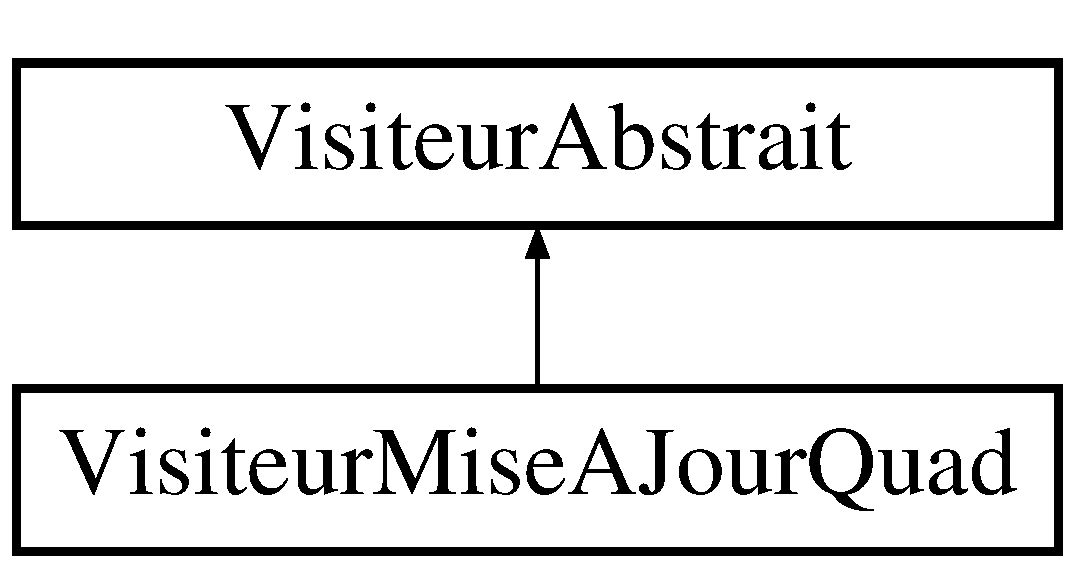
\includegraphics[height=2.000000cm]{class_visiteur_mise_a_jour_quad}
\end{center}
\end{figure}
\subsection*{Public Member Functions}
\begin{DoxyCompactItemize}
\item 
\hyperlink{group__inf2990_ga4e6fbccc3cca89891a4192a780266c60}{Visiteur\+Mise\+A\+Jour\+Quad} ()
\begin{DoxyCompactList}\small\item\em Constructeur par d�faut. \end{DoxyCompactList}\item 
virtual \hyperlink{group__inf2990_ga2f3e46969aba554699ff8e474761184f}{$\sim$\+Visiteur\+Mise\+A\+Jour\+Quad} ()
\begin{DoxyCompactList}\small\item\em Destructeur. \end{DoxyCompactList}\item 
virtual void \hyperlink{group__inf2990_gaa33f291b5fb2dee78f68a222633c2220}{visiter} (\hyperlink{class_arbre_rendu}{Arbre\+Rendu} $\ast$noeud)
\item 
virtual void \hyperlink{group__inf2990_gaa71304c2e874eee868130420c1fcaa6f}{visiter} (\hyperlink{class_noeud_table}{Noeud\+Table} $\ast$noeud)
\item 
virtual void \hyperlink{group__inf2990_ga3cc76514874afd553dbb6ed626038caf}{visiter} (\hyperlink{class_noeud_duplication}{Noeud\+Duplication} $\ast$noeud)
\item 
virtual void \hyperlink{group__inf2990_ga663ab356b2b226fb93a7900adcb46c60}{visiter} (\hyperlink{class_noeud_poteau}{Noeud\+Poteau} $\ast$noeud)
\item 
virtual void \hyperlink{group__inf2990_ga9a57770ec6f44c74b7b954eaeecd08ae}{visiter} (\hyperlink{class_noeud_mur}{Noeud\+Mur} $\ast$noeud)
\item 
virtual void \hyperlink{group__inf2990_ga3680f862903b47ab2f439e3349dc572c}{visiter} (\hyperlink{class_noeud_ligne}{Noeud\+Ligne} $\ast$noeud)
\item 
virtual void \hyperlink{group__inf2990_ga5f314c75992acc786066db96437c24ef}{visiter} (\hyperlink{class_noeud_segment}{Noeud\+Segment} $\ast$noeud)
\item 
virtual void \hyperlink{group__inf2990_gaa43c9f7c5081cf4074efc461ab551758}{visiter} (\hyperlink{class_noeud_jonction}{Noeud\+Jonction} $\ast$noeud)
\item 
virtual void \hyperlink{group__inf2990_ga363a896d920695850d6b85cef919117f}{visiter} (\hyperlink{class_noeud_depart}{Noeud\+Depart} $\ast$noeud)
\end{DoxyCompactItemize}
\subsection*{Additional Inherited Members}


\subsection{Detailed Description}
Visiteur permettant de mettre � jour la boite englobante d\textquotesingle{}un objet. 

\begin{DoxyAuthor}{Author}
Fr�d�ric Gr�goire 
\end{DoxyAuthor}
\begin{DoxyDate}{Date}
2016-\/02-\/15 
\end{DoxyDate}


The documentation for this class was generated from the following files\+:\begin{DoxyCompactItemize}
\item 
Sources/\+D\+L\+L/\+Visiteur/\hyperlink{_visiteur_mise_a_jour_quad_8h}{Visiteur\+Mise\+A\+Jour\+Quad.\+h}\item 
Sources/\+D\+L\+L/\+Visiteur/\hyperlink{_visiteur_mise_a_jour_quad_8cpp}{Visiteur\+Mise\+A\+Jour\+Quad.\+cpp}\end{DoxyCompactItemize}

\hypertarget{class_visiteur_rotation}{}\section{Visiteur\+Rotation Class Reference}
\label{class_visiteur_rotation}\index{Visiteur\+Rotation@{Visiteur\+Rotation}}


Visiteur permettant d\textquotesingle{}effectuer la rotation d\textquotesingle{}un objet.  




{\ttfamily \#include $<$Visiteur\+Rotation.\+h$>$}

Inheritance diagram for Visiteur\+Rotation\+:\begin{figure}[H]
\begin{center}
\leavevmode
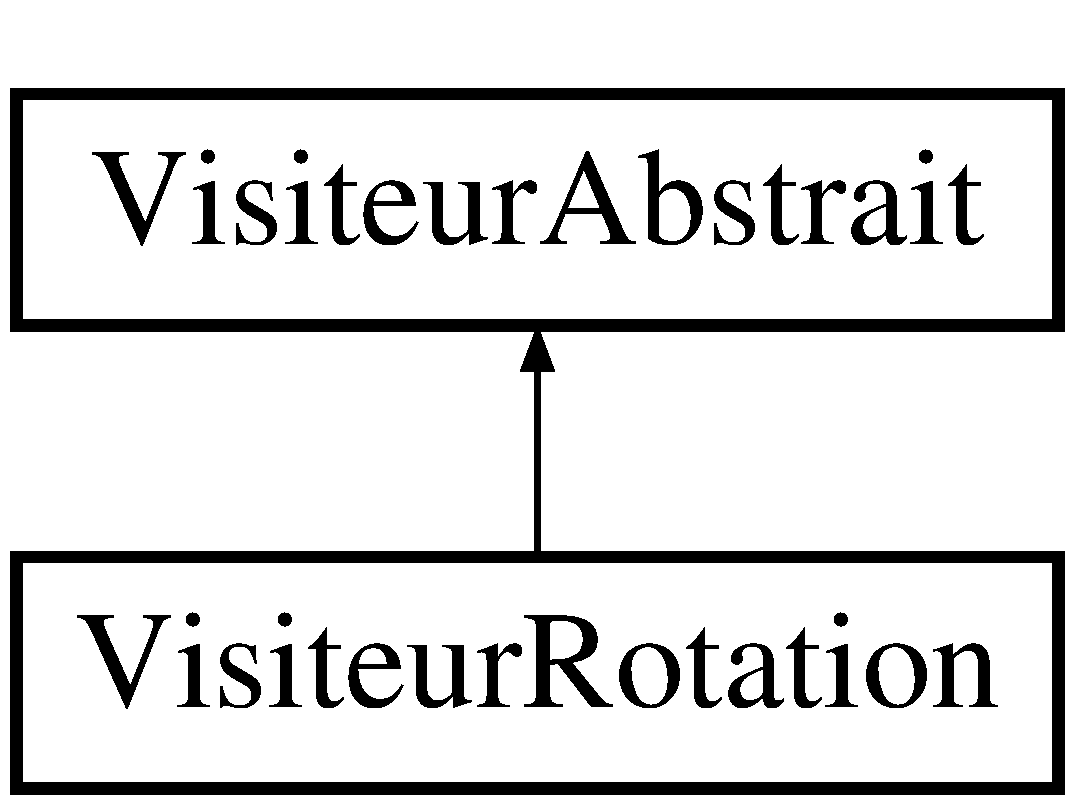
\includegraphics[height=2.000000cm]{class_visiteur_rotation}
\end{center}
\end{figure}
\subsection*{Public Member Functions}
\begin{DoxyCompactItemize}
\item 
\hyperlink{group__inf2990_ga3914046b79fcaa48a135c3026ad12f79}{Visiteur\+Rotation} ()
\begin{DoxyCompactList}\small\item\em Constructeur par d�faut. \end{DoxyCompactList}\item 
virtual \hyperlink{group__inf2990_ga6a17793fa0206b9edaa7c1e7c9bd092c}{$\sim$\+Visiteur\+Rotation} ()
\begin{DoxyCompactList}\small\item\em Destructeur. \end{DoxyCompactList}\item 
virtual void \hyperlink{group__inf2990_ga90cbfb630e4d15d5a2a5dc868e1c1433}{visiter} (\hyperlink{class_arbre_rendu}{Arbre\+Rendu} $\ast$noeud)
\item 
virtual void \hyperlink{group__inf2990_gae1865615073c00327902b12b1be14332}{visiter} (\hyperlink{class_noeud_table}{Noeud\+Table} $\ast$noeud)
\item 
virtual void \hyperlink{group__inf2990_gabdde6ab23c3353265aaec1ab31767133}{visiter} (\hyperlink{class_noeud_poteau}{Noeud\+Poteau} $\ast$noeud)
\item 
virtual void \hyperlink{group__inf2990_ga2c203c78a7dc3b9af33f348561767807}{visiter} (\hyperlink{class_noeud_mur}{Noeud\+Mur} $\ast$noeud)
\item 
virtual void \hyperlink{group__inf2990_ga33b2abf6fe078042706be105a5d01ef1}{visiter} (\hyperlink{class_noeud_ligne}{Noeud\+Ligne} $\ast$noeud)
\item 
virtual void \hyperlink{group__inf2990_gaa7b15594f39047e7e42bfa682b331225}{visiter} (\hyperlink{class_noeud_depart}{Noeud\+Depart} $\ast$noeud)
\end{DoxyCompactItemize}
\subsection*{Additional Inherited Members}


\subsection{Detailed Description}
Visiteur permettant d\textquotesingle{}effectuer la rotation d\textquotesingle{}un objet. 

\begin{DoxyAuthor}{Author}
Fr�d�ric Gr�goire 
\end{DoxyAuthor}
\begin{DoxyDate}{Date}
2016-\/02-\/15 
\end{DoxyDate}


The documentation for this class was generated from the following files\+:\begin{DoxyCompactItemize}
\item 
Sources/\+D\+L\+L/\+Visiteur/\hyperlink{_visiteur_rotation_8h}{Visiteur\+Rotation.\+h}\item 
Sources/\+D\+L\+L/\+Visiteur/\hyperlink{_visiteur_rotation_8cpp}{Visiteur\+Rotation.\+cpp}\end{DoxyCompactItemize}

\hypertarget{class_visiteur_sauvegarde}{}\section{Visiteur\+Sauvegarde Class Reference}
\label{class_visiteur_sauvegarde}\index{Visiteur\+Sauvegarde@{Visiteur\+Sauvegarde}}


Cette classe s\textquotesingle{}occupe de visiter chaque noeuds de l\textquotesingle{}arbre de rendu pour �crire leurs attributs dans un fichier Json et ainsi, permettre de les charger plus tard.  




{\ttfamily \#include $<$Visiteur\+Sauvegarde.\+h$>$}

Inheritance diagram for Visiteur\+Sauvegarde\+:\begin{figure}[H]
\begin{center}
\leavevmode
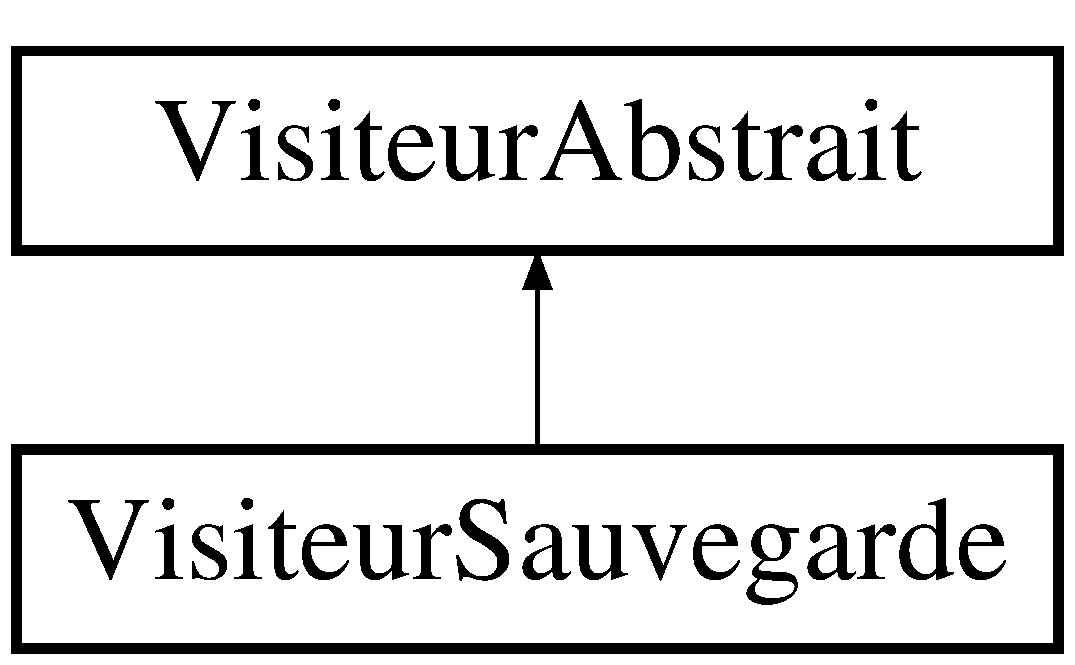
\includegraphics[height=2.000000cm]{class_visiteur_sauvegarde}
\end{center}
\end{figure}
\subsection*{Public Member Functions}
\begin{DoxyCompactItemize}
\item 
\hyperlink{group__inf2990_gab768849b68a2f0e884980110e2c082b5}{Visiteur\+Sauvegarde} ()
\begin{DoxyCompactList}\small\item\em Constructeur par d�faut. \end{DoxyCompactList}\item 
virtual \hyperlink{group__inf2990_ga8409dcc47c120f1b8511f400057e60fb}{$\sim$\+Visiteur\+Sauvegarde} ()
\begin{DoxyCompactList}\small\item\em Destructeur. \end{DoxyCompactList}\item 
virtual void \hyperlink{group__inf2990_ga0f66a9aee0e4281850944e05271f33f5}{visiter} (\hyperlink{class_arbre_rendu}{Arbre\+Rendu} $\ast$noeud)
\begin{DoxyCompactList}\small\item\em Sauvegarde en J\+S\+ON de l\textquotesingle{}arbre de rendu. \end{DoxyCompactList}\item 
virtual void \hyperlink{group__inf2990_ga12cad0534fe54c55688c66444e35a9f0}{visiter} (\hyperlink{class_noeud_table}{Noeud\+Table} $\ast$noeud)
\begin{DoxyCompactList}\small\item\em Sauvegarde en J\+S\+ON d\textquotesingle{}un \hyperlink{class_noeud_table}{Noeud\+Table}. \end{DoxyCompactList}\item 
virtual void \hyperlink{group__inf2990_gac9603c7347bdf47b429a3daed7a4194d}{visiter} (\hyperlink{class_noeud_poteau}{Noeud\+Poteau} $\ast$noeud)
\begin{DoxyCompactList}\small\item\em Sauvegarde en J\+S\+ON d\textquotesingle{}un \hyperlink{class_noeud_poteau}{Noeud\+Poteau}. \end{DoxyCompactList}\item 
virtual void \hyperlink{group__inf2990_gadda6793b1da142f5bbe9263430ea3f43}{visiter} (\hyperlink{class_noeud_mur}{Noeud\+Mur} $\ast$noeud)
\begin{DoxyCompactList}\small\item\em Sauvegarde en J\+S\+ON d\textquotesingle{}un \hyperlink{class_noeud_mur}{Noeud\+Mur}. \end{DoxyCompactList}\item 
virtual void \hyperlink{group__inf2990_gad95f454ed5389c28a91e4f387ca25bfe}{visiter} (\hyperlink{class_noeud_ligne}{Noeud\+Ligne} $\ast$noeud)
\begin{DoxyCompactList}\small\item\em Sauvegarde en J\+S\+ON d\textquotesingle{}un \hyperlink{class_noeud_ligne}{Noeud\+Ligne}. \end{DoxyCompactList}\item 
virtual void \hyperlink{group__inf2990_gafb15ac94acb1b0297ac8fdb9af8530f1}{visiter} (\hyperlink{class_noeud_segment}{Noeud\+Segment} $\ast$noeud)
\begin{DoxyCompactList}\small\item\em Sauvegarde en J\+S\+ON d\textquotesingle{}un \hyperlink{class_noeud_segment}{Noeud\+Segment}. \end{DoxyCompactList}\item 
virtual void \hyperlink{group__inf2990_ga969ffe67b3d96d9367a5b98211f80666}{visiter} (\hyperlink{class_noeud_depart}{Noeud\+Depart} $\ast$noeud)
\begin{DoxyCompactList}\small\item\em Sauvegarde en J\+S\+ON d\textquotesingle{}un \hyperlink{class_noeud_duplication}{Noeud\+Duplication}. \end{DoxyCompactList}\item 
virtual void \hyperlink{group__inf2990_ga20678afc2d407ecbe56fe54b8af6062c}{visiter} (\hyperlink{class_noeud_jonction}{Noeud\+Jonction} $\ast$noeud)
\begin{DoxyCompactList}\small\item\em Sauvegarde en J\+S\+ON d\textquotesingle{}un \hyperlink{class_noeud_duplication}{Noeud\+Duplication}. \end{DoxyCompactList}\end{DoxyCompactItemize}
\subsection*{Additional Inherited Members}


\subsection{Detailed Description}
Cette classe s\textquotesingle{}occupe de visiter chaque noeuds de l\textquotesingle{}arbre de rendu pour �crire leurs attributs dans un fichier Json et ainsi, permettre de les charger plus tard. 

\begin{DoxyAuthor}{Author}
Philippe Marcotte 
\end{DoxyAuthor}
\begin{DoxyDate}{Date}
2016-\/02-\/09 
\end{DoxyDate}


The documentation for this class was generated from the following files\+:\begin{DoxyCompactItemize}
\item 
Sources/\+D\+L\+L/\+Visiteur/\hyperlink{_visiteur_sauvegarde_8h}{Visiteur\+Sauvegarde.\+h}\item 
Sources/\+D\+L\+L/\+Visiteur/\hyperlink{_visiteur_sauvegarde_8cpp}{Visiteur\+Sauvegarde.\+cpp}\end{DoxyCompactItemize}

\hypertarget{class_visiteur_selection}{}\section{Visiteur\+Selection Class Reference}
\label{class_visiteur_selection}\index{Visiteur\+Selection@{Visiteur\+Selection}}


Visiteur permettant d\textquotesingle{}effectuer la s�lection d\textquotesingle{}un objet.  




{\ttfamily \#include $<$Visiteur\+Selection.\+h$>$}

Inheritance diagram for Visiteur\+Selection\+:\begin{figure}[H]
\begin{center}
\leavevmode
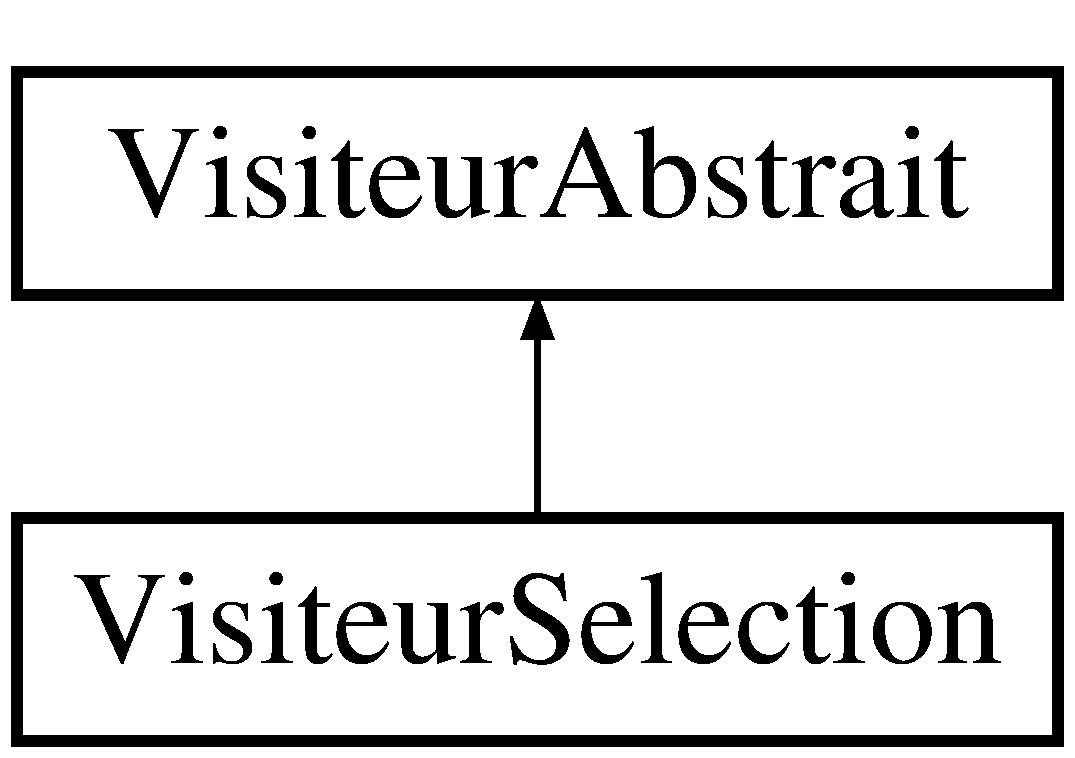
\includegraphics[height=2.000000cm]{class_visiteur_selection}
\end{center}
\end{figure}
\subsection*{Public Member Functions}
\begin{DoxyCompactItemize}
\item 
\hyperlink{group__inf2990_ga6ff39909ddbd73aa075741e617f5aa4b}{Visiteur\+Selection} ()
\begin{DoxyCompactList}\small\item\em Constructeur par d�faut. \end{DoxyCompactList}\item 
virtual \hyperlink{group__inf2990_gaf74044cdf22e6bdc2a4cd8c5afafdc60}{$\sim$\+Visiteur\+Selection} ()
\begin{DoxyCompactList}\small\item\em Destructeur. \end{DoxyCompactList}\item 
virtual void \hyperlink{group__inf2990_gabe06709bdd2c2b3c0d5536cb5622ad34}{visiter} (\hyperlink{class_arbre_rendu}{Arbre\+Rendu} $\ast$noeud)
\begin{DoxyCompactList}\small\item\em Parcours du noeud\+Table. \end{DoxyCompactList}\item 
virtual void \hyperlink{group__inf2990_ga12c860fc1d534fe9ceb5b259a9db8e7c}{visiter} (\hyperlink{class_noeud_table}{Noeud\+Table} $\ast$noeud)
\item 
virtual void \hyperlink{group__inf2990_gacfa8636c164f0e4c6dcf04b527243de0}{visiter} (\hyperlink{class_noeud_poteau}{Noeud\+Poteau} $\ast$noeud)
\item 
virtual void \hyperlink{group__inf2990_gaa5876b720f74393bf5828cee9c91b832}{visiter} (\hyperlink{class_noeud_mur}{Noeud\+Mur} $\ast$noeud)
\item 
virtual void \hyperlink{group__inf2990_gafb6006277c5a24cc3481eefb85a98391}{visiter} (\hyperlink{class_noeud_ligne}{Noeud\+Ligne} $\ast$noeud)
\item 
virtual void \hyperlink{group__inf2990_gafbc33dde6502a220782020f275896b51}{visiter} (\hyperlink{class_noeud_depart}{Noeud\+Depart} $\ast$noeud)
\item 
virtual void \hyperlink{group__inf2990_gaa0de6fd60803e1db2987d7dc67023839}{visiter} (\hyperlink{class_noeud_segment}{Noeud\+Segment} $\ast$noeud)
\item 
virtual void \hyperlink{group__inf2990_ga138fe6791d0659568518b71b4365fdd7}{visiter} (\hyperlink{class_noeud_jonction}{Noeud\+Jonction} $\ast$noeud)
\item 
void {\bfseries assigner\+Control} (bool ctrl\+Appuye)
\item 
void \hyperlink{group__inf2990_ga6f788cbce7f82a1fa7c65ae7f76b3b42}{assigner\+Position\+Rect\+Elast} (const glm\+::dvec3 \&position\+Premier\+Clic, const glm\+::dvec3 \&position\+Deuxieme\+Clic)
\item 
bool \hyperlink{group__inf2990_ga9653fe2c6211dc14b71b8523a198c599}{quad\+Est\+Dans\+Rectangle\+Elastique} (const utilitaire\+::\+Quad\+Englobant \&quad)
\end{DoxyCompactItemize}
\subsection*{Additional Inherited Members}


\subsection{Detailed Description}
Visiteur permettant d\textquotesingle{}effectuer la s�lection d\textquotesingle{}un objet. 

Visiteur permettant d\textquotesingle{}effectuer la v�rification de la boite englobante d\textquotesingle{}un objet pour qu\textquotesingle{}il soit sur la table.

\begin{DoxyAuthor}{Author}
Fr�d�ric Gr�goire 
\end{DoxyAuthor}
\begin{DoxyDate}{Date}
2016-\/02-\/15 
\end{DoxyDate}


The documentation for this class was generated from the following files\+:\begin{DoxyCompactItemize}
\item 
Sources/\+D\+L\+L/\+Visiteur/\hyperlink{_visiteur_selection_8h}{Visiteur\+Selection.\+h}\item 
Sources/\+D\+L\+L/\+Visiteur/\hyperlink{_visiteur_selection_8cpp}{Visiteur\+Selection.\+cpp}\end{DoxyCompactItemize}

\hypertarget{class_visiteur_suppression}{}\section{Visiteur\+Suppression Class Reference}
\label{class_visiteur_suppression}\index{Visiteur\+Suppression@{Visiteur\+Suppression}}


Visiteur permettant d\textquotesingle{}effectuer la supression d\textquotesingle{}un objet.  




{\ttfamily \#include $<$Visiteur\+Suppression.\+h$>$}

Inheritance diagram for Visiteur\+Suppression\+:\begin{figure}[H]
\begin{center}
\leavevmode
\includegraphics[height=2.000000cm]{class_visiteur_suppression}
\end{center}
\end{figure}
\subsection*{Public Member Functions}
\begin{DoxyCompactItemize}
\item 
\hyperlink{group__inf2990_ga77790339ddd453ed30dffccef8934373}{Visiteur\+Suppression} ()
\begin{DoxyCompactList}\small\item\em Constructeur par d�faut. \end{DoxyCompactList}\item 
virtual \hyperlink{group__inf2990_ga609bdf7e42165bdfa8d4c4d816c2b71d}{$\sim$\+Visiteur\+Suppression} ()
\begin{DoxyCompactList}\small\item\em Destructeur. \end{DoxyCompactList}\item 
virtual void \hyperlink{group__inf2990_ga438d6fdc9938649f8721cc14aa87a493}{visiter} (\hyperlink{class_noeud_table}{Noeud\+Table} $\ast$noeud)
\begin{DoxyCompactList}\small\item\em Parcours du noeud\+Table. \end{DoxyCompactList}\end{DoxyCompactItemize}
\subsection*{Additional Inherited Members}


\subsection{Detailed Description}
Visiteur permettant d\textquotesingle{}effectuer la supression d\textquotesingle{}un objet. 

\begin{DoxyAuthor}{Author}
Fr�d�ric Gr�goire 
\end{DoxyAuthor}
\begin{DoxyDate}{Date}
2016-\/02-\/15 
\end{DoxyDate}


The documentation for this class was generated from the following files\+:\begin{DoxyCompactItemize}
\item 
Sources/\+D\+L\+L/\+Visiteur/\hyperlink{_visiteur_suppression_8h}{Visiteur\+Suppression.\+h}\item 
Sources/\+D\+L\+L/\+Visiteur/\hyperlink{_visiteur_suppression_8cpp}{Visiteur\+Suppression.\+cpp}\end{DoxyCompactItemize}

\hypertarget{class_visiteur_verification_quad}{}\section{Visiteur\+Verification\+Quad Class Reference}
\label{class_visiteur_verification_quad}\index{Visiteur\+Verification\+Quad@{Visiteur\+Verification\+Quad}}
Inheritance diagram for Visiteur\+Verification\+Quad\+:\begin{figure}[H]
\begin{center}
\leavevmode
\includegraphics[height=2.000000cm]{class_visiteur_verification_quad}
\end{center}
\end{figure}
\subsection*{Public Member Functions}
\begin{DoxyCompactItemize}
\item 
\hyperlink{group__inf2990_gae4e975989da86add7de2ab4f5a19d33e}{Visiteur\+Verification\+Quad} ()
\begin{DoxyCompactList}\small\item\em Constructeur par d�faut. \end{DoxyCompactList}\item 
virtual \hyperlink{group__inf2990_gaddb978d8bbcc58899663d38616b69725}{$\sim$\+Visiteur\+Verification\+Quad} ()
\begin{DoxyCompactList}\small\item\em Destructeur. \end{DoxyCompactList}\item 
bool \hyperlink{group__inf2990_ga84aa941d923dcea87a9b7d16c2f97fea}{objets\+Dans\+Zone\+Simulation} ()
\begin{DoxyCompactList}\small\item\em Obtenir si tous les objets sont dans la zone de simulation. \end{DoxyCompactList}\item 
virtual void \hyperlink{group__inf2990_gabfdcd912f4c5672e438693f4d20434b9}{visiter} (\hyperlink{class_arbre_rendu}{Arbre\+Rendu} $\ast$noeud)
\item 
virtual void \hyperlink{group__inf2990_gae637fbd5e45449a4ce6d4876bbfdb74f}{visiter} (\hyperlink{class_noeud_table}{Noeud\+Table} $\ast$noeud)
\item 
virtual void \hyperlink{group__inf2990_ga17938068787349d67e96fe4d00d71628}{visiter} (\hyperlink{class_noeud_duplication}{Noeud\+Duplication} $\ast$noeud)
\item 
virtual void \hyperlink{group__inf2990_ga5e845f06929aa64326b3bc329aa6f7c3}{visiter} (\hyperlink{class_noeud_poteau}{Noeud\+Poteau} $\ast$noeud)
\item 
virtual void \hyperlink{group__inf2990_ga886106fc8f410bac3b634f8ad39d8ec4}{visiter} (\hyperlink{class_noeud_mur}{Noeud\+Mur} $\ast$noeud)
\item 
virtual void \hyperlink{group__inf2990_gac7da1544a08feb3f5e00bacf35006e01}{visiter} (\hyperlink{class_noeud_ligne}{Noeud\+Ligne} $\ast$noeud)
\item 
virtual void \hyperlink{group__inf2990_ga098e9c8c89a86d24a609a89abac5ee11}{visiter} (\hyperlink{class_noeud_segment}{Noeud\+Segment} $\ast$noeud)
\item 
virtual void \hyperlink{group__inf2990_ga90979a23d5385ade3e69ee362c7978db}{visiter} (\hyperlink{class_noeud_depart}{Noeud\+Depart} $\ast$noeud)
\end{DoxyCompactItemize}
\subsection*{Additional Inherited Members}


The documentation for this class was generated from the following files\+:\begin{DoxyCompactItemize}
\item 
Sources/\+D\+L\+L/\+Visiteur/\hyperlink{_visiteur_verification_quad_8h}{Visiteur\+Verification\+Quad.\+h}\item 
Sources/\+D\+L\+L/\+Visiteur/\hyperlink{_visiteur_verification_quad_8cpp}{Visiteur\+Verification\+Quad.\+cpp}\end{DoxyCompactItemize}

\hypertarget{class_interface_graphique_1_1_window}{}\section{Interface\+Graphique.\+Window Class Reference}
\label{class_interface_graphique_1_1_window}\index{Interface\+Graphique.\+Window@{Interface\+Graphique.\+Window}}
Inheritance diagram for Interface\+Graphique.\+Window\+:\begin{figure}[H]
\begin{center}
\leavevmode
\includegraphics[height=2.000000cm]{class_interface_graphique_1_1_window}
\end{center}
\end{figure}
\subsection*{Public Member Functions}
\begin{DoxyCompactItemize}
\item 
void {\bfseries arreter\+Tout\+Message} ()
\item 
bool {\bfseries Pre\+Filter\+Message} (ref Message m)
\item 
\hyperlink{group__inf2990_ga7e30ec49435f3c0fba10654f5d4c80f0}{Window} ()
\item 
void \hyperlink{group__inf2990_ga3a7a6e48395a43de034017fd06ab0b15}{Initialiser\+Animation} ()
\item 
void \hyperlink{group__inf2990_ga59ab317065d928c64d22120800595079}{Mettre\+A\+Jour} (double temps\+Inter\+Affichage)
\end{DoxyCompactItemize}
\subsection*{Protected Member Functions}
\begin{DoxyCompactItemize}
\item 
override void \hyperlink{class_interface_graphique_1_1_window_aebd9107b7e73f8a1b90129bc51bfabd9}{Dispose} (bool disposing)
\begin{DoxyCompactList}\small\item\em Nettoyage des ressources utilisées. \end{DoxyCompactList}\end{DoxyCompactItemize}


\subsection{Member Function Documentation}
\index{Interface\+Graphique\+::\+Window@{Interface\+Graphique\+::\+Window}!Dispose@{Dispose}}
\index{Dispose@{Dispose}!Interface\+Graphique\+::\+Window@{Interface\+Graphique\+::\+Window}}
\subsubsection[{\texorpdfstring{Dispose(bool disposing)}{Dispose(bool disposing)}}]{\setlength{\rightskip}{0pt plus 5cm}override void Interface\+Graphique.\+Window.\+Dispose (
\begin{DoxyParamCaption}
\item[{bool}]{disposing}
\end{DoxyParamCaption}
)\hspace{0.3cm}{\ttfamily [inline]}, {\ttfamily [protected]}}\hypertarget{class_interface_graphique_1_1_window_aebd9107b7e73f8a1b90129bc51bfabd9}{}\label{class_interface_graphique_1_1_window_aebd9107b7e73f8a1b90129bc51bfabd9}


Nettoyage des ressources utilisées. 


\begin{DoxyParams}{Parameters}
{\em disposing} & true si les ressources managées doivent être supprimées ; sinon, false.\\
\hline
\end{DoxyParams}


The documentation for this class was generated from the following files\+:\begin{DoxyCompactItemize}
\item 
Sources/\+Interface\+Graphique/\hyperlink{_window_8cs}{Window.\+cs}\item 
Sources/\+Interface\+Graphique/Window.\+Designer.\+cs\end{DoxyCompactItemize}

\chapter{File Documentation}
\hypertarget{_facade_modele_8cpp}{}\section{Sources/\+D\+L\+L/\+Application/\+Facade\+Modele.cpp File Reference}
\label{_facade_modele_8cpp}\index{Sources/\+D\+L\+L/\+Application/\+Facade\+Modele.\+cpp@{Sources/\+D\+L\+L/\+Application/\+Facade\+Modele.\+cpp}}
{\ttfamily \#include $<$windows.\+h$>$}\\*
{\ttfamily \#include $<$cassert$>$}\\*
{\ttfamily \#include \char`\"{}G\+L/glew.\+h\char`\"{}}\\*
{\ttfamily \#include \char`\"{}Free\+Image.\+h\char`\"{}}\\*
{\ttfamily \#include \char`\"{}Facade\+Modele.\+h\char`\"{}}\\*
{\ttfamily \#include \char`\"{}Vue\+Ortho.\+h\char`\"{}}\\*
{\ttfamily \#include \char`\"{}Camera.\+h\char`\"{}}\\*
{\ttfamily \#include \char`\"{}Projection.\+h\char`\"{}}\\*
{\ttfamily \#include \char`\"{}Utilitaire.\+h\char`\"{}}\\*
{\ttfamily \#include \char`\"{}Aide\+G\+L.\+h\char`\"{}}\\*
{\ttfamily \#include \char`\"{}Arbre\+Rendu\+I\+N\+F2990.\+h\char`\"{}}\\*
{\ttfamily \#include \char`\"{}Config\+Scene.\+h\char`\"{}}\\*
{\ttfamily \#include \char`\"{}Compteur\+Affichage.\+h\char`\"{}}\\*
{\ttfamily \#include \char`\"{}tinyxml2.\+h\char`\"{}}\\*
{\ttfamily \#include \char`\"{}glm/glm.\+hpp\char`\"{}}\\*
{\ttfamily \#include \char`\"{}glm/gtc/type\+\_\+ptr.\+hpp\char`\"{}}\\*
{\ttfamily \#include \char`\"{}Etat\+Types.\+h\char`\"{}}\\*
{\ttfamily \#include \char`\"{}Mode\+Types.\+h\char`\"{}}\\*


\subsection{Detailed Description}
\begin{DoxyAuthor}{Author}
Martin Bisson 
\end{DoxyAuthor}
\begin{DoxyDate}{Date}
2007-\/05-\/22 
\end{DoxyDate}
\begin{DoxyVersion}{Version}
1.\+0 
\end{DoxyVersion}

\hypertarget{_facade_modele_8h}{}\section{Sources/\+D\+L\+L/\+Application/\+Facade\+Modele.h File Reference}
\label{_facade_modele_8h}\index{Sources/\+D\+L\+L/\+Application/\+Facade\+Modele.\+h@{Sources/\+D\+L\+L/\+Application/\+Facade\+Modele.\+h}}
{\ttfamily \#include $<$windows.\+h$>$}\\*
{\ttfamily \#include $<$string$>$}\\*
{\ttfamily \#include $<$memory$>$}\\*
{\ttfamily \#include \char`\"{}Vue.\+h\char`\"{}}\\*
{\ttfamily \#include \char`\"{}Arbre\+Rendu\+I\+N\+F2990.\+h\char`\"{}}\\*
{\ttfamily \#include \char`\"{}Etat\+Abstrait.\+h\char`\"{}}\\*
{\ttfamily \#include \char`\"{}Mode\+Abstrait.\+h\char`\"{}}\\*
\subsection*{Classes}
\begin{DoxyCompactItemize}
\item 
class \hyperlink{class_facade_modele}{Facade\+Modele}
\begin{DoxyCompactList}\small\item\em Classe qui constitue une interface (une fa�ade) sur l\textquotesingle{}ensemble du mod�le et des classes qui le composent. \end{DoxyCompactList}\end{DoxyCompactItemize}


\subsection{Detailed Description}
\begin{DoxyAuthor}{Author}
D\+GI 
\end{DoxyAuthor}
\begin{DoxyDate}{Date}
2005-\/06-\/15 
\end{DoxyDate}
\begin{DoxyVersion}{Version}
1.\+0 
\end{DoxyVersion}

\hypertarget{_arbre_rendu_8cpp}{}\section{Sources/\+D\+L\+L/\+Arbre/\+Arbre\+Rendu.cpp File Reference}
\label{_arbre_rendu_8cpp}\index{Sources/\+D\+L\+L/\+Arbre/\+Arbre\+Rendu.\+cpp@{Sources/\+D\+L\+L/\+Arbre/\+Arbre\+Rendu.\+cpp}}
{\ttfamily \#include \char`\"{}Arbre\+Rendu.\+h\char`\"{}}\\*
{\ttfamily \#include \char`\"{}Usine\+Noeud.\+h\char`\"{}}\\*
{\ttfamily \#include \char`\"{}Noeud\+Abstrait.\+h\char`\"{}}\\*
{\ttfamily \#include \char`\"{}Visiteur\+Abstrait.\+h\char`\"{}}\\*
{\ttfamily \#include \char`\"{}G\+L/glew.\+h\char`\"{}}\\*


\subsection{Detailed Description}
\begin{DoxyAuthor}{Author}
Martin Bisson 
\end{DoxyAuthor}
\begin{DoxyDate}{Date}
2007-\/01-\/28 
\end{DoxyDate}

\hypertarget{_arbre_rendu_8h}{}\section{Sources/\+D\+L\+L/\+Arbre/\+Arbre\+Rendu.h File Reference}
\label{_arbre_rendu_8h}\index{Sources/\+D\+L\+L/\+Arbre/\+Arbre\+Rendu.\+h@{Sources/\+D\+L\+L/\+Arbre/\+Arbre\+Rendu.\+h}}
{\ttfamily \#include \char`\"{}Noeud\+Composite.\+h\char`\"{}}\\*
{\ttfamily \#include $<$map$>$}\\*
{\ttfamily \#include $<$memory$>$}\\*
{\ttfamily \#include \char`\"{}Usine\+Noeud.\+h\char`\"{}}\\*
\subsection*{Classes}
\begin{DoxyCompactItemize}
\item 
class \hyperlink{class_arbre_rendu}{Arbre\+Rendu}
\begin{DoxyCompactList}\small\item\em Classe d\textquotesingle{}arbre de rendu qui contient la racine de l\textquotesingle{}arbre de rendu avec les usines qui permettent d\textquotesingle{}ajouter des noeuds � cet arbre. \end{DoxyCompactList}\end{DoxyCompactItemize}


\subsection{Detailed Description}
\begin{DoxyAuthor}{Author}
Martin Bisson 
\end{DoxyAuthor}
\begin{DoxyDate}{Date}
2007-\/01-\/28 
\end{DoxyDate}
\begin{DoxyVersion}{Version}
1.\+0 
\end{DoxyVersion}

\hypertarget{_arbre_rendu_i_n_f2990_8cpp}{}\section{Sources/\+D\+L\+L/\+Arbre/\+Arbre\+Rendu\+I\+N\+F2990.cpp File Reference}
\label{_arbre_rendu_i_n_f2990_8cpp}\index{Sources/\+D\+L\+L/\+Arbre/\+Arbre\+Rendu\+I\+N\+F2990.\+cpp@{Sources/\+D\+L\+L/\+Arbre/\+Arbre\+Rendu\+I\+N\+F2990.\+cpp}}
{\ttfamily \#include \char`\"{}Arbre\+Rendu\+I\+N\+F2990.\+h\char`\"{}}\\*
{\ttfamily \#include \char`\"{}Usines/\+Usine\+Noeud.\+h\char`\"{}}\\*
{\ttfamily \#include \char`\"{}Etat\+Open\+G\+L.\+h\char`\"{}}\\*
{\ttfamily \#include \char`\"{}Noeud\+Types.\+h\char`\"{}}\\*
{\ttfamily \#include \char`\"{}Visiteur\+Types.\+h\char`\"{}}\\*
{\ttfamily \#include $<$stdio.\+h$>$}\\*
{\ttfamily \#include \char`\"{}rapidjson\textbackslash{}filereadstream.\+h\char`\"{}}\\*
{\ttfamily \#include $<$sys/stat.\+h$>$}\\*
{\ttfamily \#include $<$windows.\+h$>$}\\*
{\ttfamily \#include $<$locale$>$}\\*
{\ttfamily \#include $<$codecvt$>$}\\*
{\ttfamily \#include $<$string$>$}\\*


\subsection{Detailed Description}
\begin{DoxyAuthor}{Author}
Martin Bisson 
\end{DoxyAuthor}
\begin{DoxyDate}{Date}
2007-\/03-\/23 
\end{DoxyDate}
\begin{DoxyVersion}{Version}
1.\+0 
\end{DoxyVersion}

\hypertarget{_arbre_rendu_i_n_f2990_8h}{}\section{Sources/\+D\+L\+L/\+Arbre/\+Arbre\+Rendu\+I\+N\+F2990.h File Reference}
\label{_arbre_rendu_i_n_f2990_8h}\index{Sources/\+D\+L\+L/\+Arbre/\+Arbre\+Rendu\+I\+N\+F2990.\+h@{Sources/\+D\+L\+L/\+Arbre/\+Arbre\+Rendu\+I\+N\+F2990.\+h}}
{\ttfamily \#include \char`\"{}Arbre\+Rendu.\+h\char`\"{}}\\*
{\ttfamily \#include $<$map$>$}\\*
{\ttfamily \#include $<$string$>$}\\*
{\ttfamily \#include \char`\"{}rapidjson\textbackslash{}document.\+h\char`\"{}}\\*
\subsection*{Classes}
\begin{DoxyCompactItemize}
\item 
class \hyperlink{class_arbre_rendu_i_n_f2990}{Arbre\+Rendu\+I\+N\+F2990}
\begin{DoxyCompactList}\small\item\em Classe qui repr�sente l\textquotesingle{}arbre de rendu sp�cifique au projet de I\+N\+F2990. \end{DoxyCompactList}\end{DoxyCompactItemize}


\subsection{Detailed Description}
\begin{DoxyAuthor}{Author}
Martin Bisson 
\end{DoxyAuthor}
\begin{DoxyDate}{Date}
2007-\/03-\/23 
\end{DoxyDate}
\begin{DoxyVersion}{Version}
1.\+0 
\end{DoxyVersion}

\hypertarget{_noeud_abstrait_8cpp}{}\section{Sources/\+D\+L\+L/\+Arbre/\+Noeuds/\+Noeud\+Abstrait.cpp File Reference}
\label{_noeud_abstrait_8cpp}\index{Sources/\+D\+L\+L/\+Arbre/\+Noeuds/\+Noeud\+Abstrait.\+cpp@{Sources/\+D\+L\+L/\+Arbre/\+Noeuds/\+Noeud\+Abstrait.\+cpp}}
{\ttfamily \#include \char`\"{}Noeud\+Abstrait.\+h\char`\"{}}\\*
{\ttfamily \#include \char`\"{}Utilitaire.\+h\char`\"{}}\\*
{\ttfamily \#include $<$iterator$>$}\\*
{\ttfamily \#include \char`\"{}rapidjson\textbackslash{}filewritestream.\+h\char`\"{}}\\*
{\ttfamily \#include $<$iostream$>$}\\*


\subsection{Detailed Description}
\begin{DoxyAuthor}{Author}
D\+G\+I-\/2990 
\end{DoxyAuthor}
\begin{DoxyDate}{Date}
2007-\/01-\/24 
\end{DoxyDate}

\hypertarget{_noeud_abstrait_8h}{}\section{Sources/\+D\+L\+L/\+Arbre/\+Noeuds/\+Noeud\+Abstrait.h File Reference}
\label{_noeud_abstrait_8h}\index{Sources/\+D\+L\+L/\+Arbre/\+Noeuds/\+Noeud\+Abstrait.\+h@{Sources/\+D\+L\+L/\+Arbre/\+Noeuds/\+Noeud\+Abstrait.\+h}}
{\ttfamily \#include \char`\"{}G\+L/glew.\+h\char`\"{}}\\*
{\ttfamily \#include $<$string$>$}\\*
{\ttfamily \#include $<$memory$>$}\\*
{\ttfamily \#include $<$iterator$>$}\\*
{\ttfamily \#include \char`\"{}Utilitaire.\+h\char`\"{}}\\*
{\ttfamily \#include \char`\"{}glm\textbackslash{}glm.\+hpp\char`\"{}}\\*
{\ttfamily \#include \char`\"{}rapidjson\textbackslash{}writer.\+h\char`\"{}}\\*
{\ttfamily \#include \char`\"{}rapidjson\textbackslash{}document.\+h\char`\"{}}\\*
\subsection*{Classes}
\begin{DoxyCompactItemize}
\item 
class \hyperlink{class_noeud_abstrait}{Noeud\+Abstrait}
\begin{DoxyCompactList}\small\item\em Classe de base du patron composite utilis�e pour cr�er l\textquotesingle{}arbre de rendu. \end{DoxyCompactList}\end{DoxyCompactItemize}
\subsection*{Namespaces}
\begin{DoxyCompactItemize}
\item 
 \hyperlink{namespacemodele}{modele}
\begin{DoxyCompactList}\small\item\em D�clarations avanc�es pour contenir un pointeur vers un mod�le3D et son storage. \end{DoxyCompactList}\end{DoxyCompactItemize}


\subsection{Detailed Description}
\begin{DoxyAuthor}{Author}
D\+G\+I-\/\+I\+N\+F2990 
\end{DoxyAuthor}
\begin{DoxyDate}{Date}
2007-\/01-\/24 
\end{DoxyDate}
\begin{DoxyVersion}{Version}
1.\+0 
\end{DoxyVersion}

\hypertarget{_noeud_composite_8cpp}{}\section{Sources/\+D\+L\+L/\+Arbre/\+Noeuds/\+Noeud\+Composite.cpp File Reference}
\label{_noeud_composite_8cpp}\index{Sources/\+D\+L\+L/\+Arbre/\+Noeuds/\+Noeud\+Composite.\+cpp@{Sources/\+D\+L\+L/\+Arbre/\+Noeuds/\+Noeud\+Composite.\+cpp}}
{\ttfamily \#include \char`\"{}Noeud\+Composite.\+h\char`\"{}}\\*
{\ttfamily \#include $<$cassert$>$}\\*


\subsection{Detailed Description}
\begin{DoxyAuthor}{Author}
D\+G\+I-\/2990 
\end{DoxyAuthor}
\begin{DoxyDate}{Date}
2007-\/01-\/25 
\end{DoxyDate}

\hypertarget{_noeud_composite_8h}{}\section{Sources/\+D\+L\+L/\+Arbre/\+Noeuds/\+Noeud\+Composite.h File Reference}
\label{_noeud_composite_8h}\index{Sources/\+D\+L\+L/\+Arbre/\+Noeuds/\+Noeud\+Composite.\+h@{Sources/\+D\+L\+L/\+Arbre/\+Noeuds/\+Noeud\+Composite.\+h}}
{\ttfamily \#include \char`\"{}Noeud\+Abstrait.\+h\char`\"{}}\\*
{\ttfamily \#include $<$vector$>$}\\*
\subsection*{Classes}
\begin{DoxyCompactItemize}
\item 
class \hyperlink{class_noeud_composite}{Noeud\+Composite}
\begin{DoxyCompactList}\small\item\em Implantation d\textquotesingle{}un noeud du patron composite qui peut poss�der des enfants. \end{DoxyCompactList}\end{DoxyCompactItemize}


\subsection{Detailed Description}
\begin{DoxyAuthor}{Author}
D\+G\+I-\/\+I\+N\+F2990 
\end{DoxyAuthor}
\begin{DoxyDate}{Date}
2007-\/01-\/25 
\end{DoxyDate}
\begin{DoxyVersion}{Version}
1.\+0 
\end{DoxyVersion}

\hypertarget{_noeud_depart_8cpp}{}\section{Sources/\+D\+L\+L/\+Arbre/\+Noeuds/\+Noeud\+Depart.cpp File Reference}
\label{_noeud_depart_8cpp}\index{Sources/\+D\+L\+L/\+Arbre/\+Noeuds/\+Noeud\+Depart.\+cpp@{Sources/\+D\+L\+L/\+Arbre/\+Noeuds/\+Noeud\+Depart.\+cpp}}
{\ttfamily \#include \char`\"{}Noeud\+Depart.\+h\char`\"{}}\\*
{\ttfamily \#include \char`\"{}Utilitaire.\+h\char`\"{}}\\*
{\ttfamily \#include \char`\"{}G\+L/glew.\+h\char`\"{}}\\*
{\ttfamily \#include $<$cmath$>$}\\*
{\ttfamily \#include \char`\"{}Modele3\+D.\+h\char`\"{}}\\*
{\ttfamily \#include \char`\"{}Open\+G\+L\+\_\+\+V\+B\+O.\+h\char`\"{}}\\*
{\ttfamily \#include \char`\"{}Visiteur\+Abstrait.\+h\char`\"{}}\\*


\subsection{Detailed Description}
\begin{DoxyAuthor}{Author}
Fr�d�ric Gr�goire 
\end{DoxyAuthor}
\begin{DoxyDate}{Date}
2011-\/05-\/19 
\end{DoxyDate}
\begin{DoxyVersion}{Version}
1.\+0 
\end{DoxyVersion}

\hypertarget{_noeud_depart_8h}{}\section{Sources/\+D\+L\+L/\+Arbre/\+Noeuds/\+Noeud\+Depart.h File Reference}
\label{_noeud_depart_8h}\index{Sources/\+D\+L\+L/\+Arbre/\+Noeuds/\+Noeud\+Depart.\+h@{Sources/\+D\+L\+L/\+Arbre/\+Noeuds/\+Noeud\+Depart.\+h}}
{\ttfamily \#include \char`\"{}Noeud\+Composite.\+h\char`\"{}}\\*
{\ttfamily \#include \char`\"{}G\+L/glew.\+h\char`\"{}}\\*
\subsection*{Classes}
\begin{DoxyCompactItemize}
\item 
class \hyperlink{class_noeud_depart}{Noeud\+Depart}
\begin{DoxyCompactList}\small\item\em Classe qui repr�sente le point d�part du robot lors de la simulation. \end{DoxyCompactList}\end{DoxyCompactItemize}


\subsection{Detailed Description}
\begin{DoxyAuthor}{Author}
Fr�d�ric Gr�goire 
\end{DoxyAuthor}
\begin{DoxyDate}{Date}
2016-\/02-\/10 
\end{DoxyDate}
\begin{DoxyVersion}{Version}
1.\+0 
\end{DoxyVersion}

\hypertarget{_noeud_duplication_8cpp}{}\section{Sources/\+D\+L\+L/\+Arbre/\+Noeuds/\+Noeud\+Duplication.cpp File Reference}
\label{_noeud_duplication_8cpp}\index{Sources/\+D\+L\+L/\+Arbre/\+Noeuds/\+Noeud\+Duplication.\+cpp@{Sources/\+D\+L\+L/\+Arbre/\+Noeuds/\+Noeud\+Duplication.\+cpp}}
{\ttfamily \#include \char`\"{}Noeud\+Duplication.\+h\char`\"{}}\\*
{\ttfamily \#include \char`\"{}Visiteur\+Abstrait.\+h\char`\"{}}\\*


\subsection{Detailed Description}
\begin{DoxyAuthor}{Author}
Olivier St-\/\+Amour 
\end{DoxyAuthor}
\begin{DoxyDate}{Date}
2016-\/02-\/10 
\end{DoxyDate}
\begin{DoxyVersion}{Version}
1.\+0 
\end{DoxyVersion}

\hypertarget{_noeud_duplication_8h}{}\section{Sources/\+D\+L\+L/\+Arbre/\+Noeuds/\+Noeud\+Duplication.h File Reference}
\label{_noeud_duplication_8h}\index{Sources/\+D\+L\+L/\+Arbre/\+Noeuds/\+Noeud\+Duplication.\+h@{Sources/\+D\+L\+L/\+Arbre/\+Noeuds/\+Noeud\+Duplication.\+h}}
{\ttfamily \#include \char`\"{}Noeud\+Composite.\+h\char`\"{}}\\*
{\ttfamily \#include \char`\"{}G\+L/glew.\+h\char`\"{}}\\*
\subsection*{Classes}
\begin{DoxyCompactItemize}
\item 
class \hyperlink{class_noeud_duplication}{Noeud\+Duplication}
\begin{DoxyCompactList}\small\item\em Noeud qui repr�sente une duplication lors de l\textquotesingle{}utilisation de l\textquotesingle{}outil duplication. \end{DoxyCompactList}\end{DoxyCompactItemize}


\subsection{Detailed Description}
\begin{DoxyAuthor}{Author}
Olivier St-\/\+Amour 
\end{DoxyAuthor}
\begin{DoxyDate}{Date}
2016-\/02-\/02 
\end{DoxyDate}
\begin{DoxyVersion}{Version}
1.\+0 
\end{DoxyVersion}

\hypertarget{_noeud_jonction_8h}{}\section{Sources/\+D\+L\+L/\+Arbre/\+Noeuds/\+Noeud\+Jonction.h File Reference}
\label{_noeud_jonction_8h}\index{Sources/\+D\+L\+L/\+Arbre/\+Noeuds/\+Noeud\+Jonction.\+h@{Sources/\+D\+L\+L/\+Arbre/\+Noeuds/\+Noeud\+Jonction.\+h}}
{\ttfamily \#include \char`\"{}Noeud\+Composite.\+h\char`\"{}}\\*
{\ttfamily \#include \char`\"{}G\+L/glew.\+h\char`\"{}}\\*
\subsection*{Classes}
\begin{DoxyCompactItemize}
\item 
class \hyperlink{class_noeud_jonction}{Noeud\+Jonction}
\begin{DoxyCompactList}\small\item\em Noeud de l\textquotesingle{}objet rendu servant � la liaison de segments de la ligne noire. \end{DoxyCompactList}\end{DoxyCompactItemize}


\subsection{Detailed Description}
\begin{DoxyAuthor}{Author}
Camille Gendreau 
\end{DoxyAuthor}
\begin{DoxyDate}{Date}
2016-\/02-\/11 
\end{DoxyDate}
\begin{DoxyVersion}{Version}
1.\+0 
\end{DoxyVersion}

\hypertarget{_noeud_ligne_8cpp}{}\section{Sources/\+D\+L\+L/\+Arbre/\+Noeuds/\+Noeud\+Ligne.cpp File Reference}
\label{_noeud_ligne_8cpp}\index{Sources/\+D\+L\+L/\+Arbre/\+Noeuds/\+Noeud\+Ligne.\+cpp@{Sources/\+D\+L\+L/\+Arbre/\+Noeuds/\+Noeud\+Ligne.\+cpp}}
{\ttfamily \#include \char`\"{}Noeud\+Ligne.\+h\char`\"{}}\\*
{\ttfamily \#include \char`\"{}Utilitaire.\+h\char`\"{}}\\*
{\ttfamily \#include \char`\"{}G\+L/glew.\+h\char`\"{}}\\*
{\ttfamily \#include $<$cmath$>$}\\*
{\ttfamily \#include \char`\"{}Modele3\+D.\+h\char`\"{}}\\*
{\ttfamily \#include \char`\"{}Open\+G\+L\+\_\+\+V\+B\+O.\+h\char`\"{}}\\*
{\ttfamily \#include \char`\"{}Visiteur\+Abstrait.\+h\char`\"{}}\\*


\subsection{Detailed Description}
\begin{DoxyAuthor}{Author}
Frederic Gregoire 
\end{DoxyAuthor}
\begin{DoxyDate}{Date}
2011-\/05-\/19 
\end{DoxyDate}
\begin{DoxyVersion}{Version}
1.\+0 
\end{DoxyVersion}

\hypertarget{_noeud_ligne_8h}{}\section{Sources/\+D\+L\+L/\+Arbre/\+Noeuds/\+Noeud\+Ligne.h File Reference}
\label{_noeud_ligne_8h}\index{Sources/\+D\+L\+L/\+Arbre/\+Noeuds/\+Noeud\+Ligne.\+h@{Sources/\+D\+L\+L/\+Arbre/\+Noeuds/\+Noeud\+Ligne.\+h}}
{\ttfamily \#include \char`\"{}Noeud\+Composite.\+h\char`\"{}}\\*
{\ttfamily \#include \char`\"{}G\+L/glew.\+h\char`\"{}}\\*
\subsection*{Classes}
\begin{DoxyCompactItemize}
\item 
class \hyperlink{class_noeud_ligne}{Noeud\+Ligne}
\begin{DoxyCompactList}\small\item\em Noeud de l\textquotesingle{}objet englobant tous les segments et jonctions d\textquotesingle{}une ligne noire. \end{DoxyCompactList}\end{DoxyCompactItemize}


\subsection{Detailed Description}
\begin{DoxyAuthor}{Author}
Frederic Gregoire 
\end{DoxyAuthor}
\begin{DoxyDate}{Date}
2016-\/01-\/20 
\end{DoxyDate}
\begin{DoxyVersion}{Version}
1.\+0 
\end{DoxyVersion}

\hypertarget{_noeud_mur_8cpp}{}\section{Sources/\+D\+L\+L/\+Arbre/\+Noeuds/\+Noeud\+Mur.cpp File Reference}
\label{_noeud_mur_8cpp}\index{Sources/\+D\+L\+L/\+Arbre/\+Noeuds/\+Noeud\+Mur.\+cpp@{Sources/\+D\+L\+L/\+Arbre/\+Noeuds/\+Noeud\+Mur.\+cpp}}
{\ttfamily \#include \char`\"{}Noeud\+Mur.\+h\char`\"{}}\\*
{\ttfamily \#include \char`\"{}Utilitaire.\+h\char`\"{}}\\*
{\ttfamily \#include \char`\"{}G\+L/glew.\+h\char`\"{}}\\*
{\ttfamily \#include $<$cmath$>$}\\*
{\ttfamily \#include \char`\"{}Modele3\+D.\+h\char`\"{}}\\*
{\ttfamily \#include \char`\"{}Open\+G\+L\+\_\+\+V\+B\+O.\+h\char`\"{}}\\*
{\ttfamily \#include \char`\"{}Visiteur\+Abstrait.\+h\char`\"{}}\\*


\subsection{Detailed Description}
\begin{DoxyAuthor}{Author}
Philippe Marcotte et Camille Gendreau 
\end{DoxyAuthor}
\begin{DoxyDate}{Date}
2016-\/05-\/19 
\end{DoxyDate}
\begin{DoxyVersion}{Version}
1.\+0 
\end{DoxyVersion}

\hypertarget{_noeud_mur_8h}{}\section{Sources/\+D\+L\+L/\+Arbre/\+Noeuds/\+Noeud\+Mur.h File Reference}
\label{_noeud_mur_8h}\index{Sources/\+D\+L\+L/\+Arbre/\+Noeuds/\+Noeud\+Mur.\+h@{Sources/\+D\+L\+L/\+Arbre/\+Noeuds/\+Noeud\+Mur.\+h}}
{\ttfamily \#include \char`\"{}Noeud\+Composite.\+h\char`\"{}}\\*
{\ttfamily \#include \char`\"{}G\+L/glew.\+h\char`\"{}}\\*
\subsection*{Classes}
\begin{DoxyCompactItemize}
\item 
class \hyperlink{class_noeud_mur}{Noeud\+Mur}
\end{DoxyCompactItemize}


\subsection{Detailed Description}
\begin{DoxyAuthor}{Author}
Frederic Gregoire 
\end{DoxyAuthor}
\begin{DoxyDate}{Date}
2016-\/01-\/20 
\end{DoxyDate}
\begin{DoxyVersion}{Version}
1.\+0 
\end{DoxyVersion}

\hypertarget{_noeud_poteau_8cpp}{}\section{Sources/\+D\+L\+L/\+Arbre/\+Noeuds/\+Noeud\+Poteau.cpp File Reference}
\label{_noeud_poteau_8cpp}\index{Sources/\+D\+L\+L/\+Arbre/\+Noeuds/\+Noeud\+Poteau.\+cpp@{Sources/\+D\+L\+L/\+Arbre/\+Noeuds/\+Noeud\+Poteau.\+cpp}}
{\ttfamily \#include \char`\"{}Noeud\+Poteau.\+h\char`\"{}}\\*
{\ttfamily \#include \char`\"{}Utilitaire.\+h\char`\"{}}\\*
{\ttfamily \#include \char`\"{}G\+L/glew.\+h\char`\"{}}\\*
{\ttfamily \#include $<$cmath$>$}\\*
{\ttfamily \#include $<$iostream$>$}\\*
{\ttfamily \#include \char`\"{}Modele3\+D.\+h\char`\"{}}\\*
{\ttfamily \#include \char`\"{}Open\+G\+L\+\_\+\+V\+B\+O.\+h\char`\"{}}\\*
{\ttfamily \#include \char`\"{}Visiteur\+Abstrait.\+h\char`\"{}}\\*


\subsection{Detailed Description}
\begin{DoxyAuthor}{Author}
Camille Gendreau 
\end{DoxyAuthor}
\begin{DoxyDate}{Date}
2016-\/02-\/11 
\end{DoxyDate}
\begin{DoxyVersion}{Version}
1.\+0
\end{DoxyVersion}
\begin{DoxyAuthor}{Author}
Philippe Marcotte et Camille Gendreau 
\end{DoxyAuthor}
\begin{DoxyDate}{Date}
2011-\/05-\/19 
\end{DoxyDate}
\begin{DoxyVersion}{Version}
1.\+0 
\end{DoxyVersion}

\hypertarget{_noeud_poteau_8h}{}\section{Sources/\+D\+L\+L/\+Arbre/\+Noeuds/\+Noeud\+Poteau.h File Reference}
\label{_noeud_poteau_8h}\index{Sources/\+D\+L\+L/\+Arbre/\+Noeuds/\+Noeud\+Poteau.\+h@{Sources/\+D\+L\+L/\+Arbre/\+Noeuds/\+Noeud\+Poteau.\+h}}
{\ttfamily \#include \char`\"{}Noeud\+Composite.\+h\char`\"{}}\\*
{\ttfamily \#include \char`\"{}G\+L/glew.\+h\char`\"{}}\\*
\subsection*{Classes}
\begin{DoxyCompactItemize}
\item 
class \hyperlink{class_noeud_poteau}{Noeud\+Poteau}
\begin{DoxyCompactList}\small\item\em Noeud des obstacles au robot sous forme de poteaux. \end{DoxyCompactList}\end{DoxyCompactItemize}


\subsection{Detailed Description}
\begin{DoxyAuthor}{Author}
Frederic Gregoire 
\end{DoxyAuthor}
\begin{DoxyDate}{Date}
2016-\/01-\/20 
\end{DoxyDate}
\begin{DoxyVersion}{Version}
1.\+0 
\end{DoxyVersion}

\hypertarget{_noeud_robot_8cpp}{}\section{Sources/\+D\+L\+L/\+Arbre/\+Noeuds/\+Noeud\+Robot.cpp File Reference}
\label{_noeud_robot_8cpp}\index{Sources/\+D\+L\+L/\+Arbre/\+Noeuds/\+Noeud\+Robot.\+cpp@{Sources/\+D\+L\+L/\+Arbre/\+Noeuds/\+Noeud\+Robot.\+cpp}}
{\ttfamily \#include \char`\"{}Noeud\+Robot.\+h\char`\"{}}\\*
{\ttfamily \#include \char`\"{}Utilitaire.\+h\char`\"{}}\\*
{\ttfamily \#include \char`\"{}Visiteur\+Abstrait.\+h\char`\"{}}\\*
{\ttfamily \#include \char`\"{}G\+L/glew.\+h\char`\"{}}\\*
{\ttfamily \#include $<$cmath$>$}\\*
{\ttfamily \#include \char`\"{}Modele3\+D.\+h\char`\"{}}\\*
{\ttfamily \#include \char`\"{}Open\+G\+L\+\_\+\+V\+B\+O.\+h\char`\"{}}\\*


\subsection{Detailed Description}
\begin{DoxyAuthor}{Author}
Martin Paradis 
\end{DoxyAuthor}
\begin{DoxyDate}{Date}
2015-\/08-\/30 
\end{DoxyDate}
\begin{DoxyVersion}{Version}
1.\+0 
\end{DoxyVersion}

\hypertarget{_noeud_robot_8h}{}\section{Sources/\+D\+L\+L/\+Arbre/\+Noeuds/\+Noeud\+Robot.h File Reference}
\label{_noeud_robot_8h}\index{Sources/\+D\+L\+L/\+Arbre/\+Noeuds/\+Noeud\+Robot.\+h@{Sources/\+D\+L\+L/\+Arbre/\+Noeuds/\+Noeud\+Robot.\+h}}
{\ttfamily \#include \char`\"{}Noeud\+Composite.\+h\char`\"{}}\\*
{\ttfamily \#include \char`\"{}G\+L/glew.\+h\char`\"{}}\\*
\subsection*{Classes}
\begin{DoxyCompactItemize}
\item 
class \hyperlink{class_noeud_robot}{Noeud\+Robot}
\begin{DoxyCompactList}\small\item\em Classe qui repr�sente le robot du premier projet int�grateur. \end{DoxyCompactList}\end{DoxyCompactItemize}


\subsection{Detailed Description}
\begin{DoxyAuthor}{Author}
Martin Paradis 
\end{DoxyAuthor}
\begin{DoxyDate}{Date}
2015-\/08-\/30 
\end{DoxyDate}
\begin{DoxyVersion}{Version}
1.\+0 
\end{DoxyVersion}

\hypertarget{_noeud_segment_8cpp}{}\section{Sources/\+D\+L\+L/\+Arbre/\+Noeuds/\+Noeud\+Segment.cpp File Reference}
\label{_noeud_segment_8cpp}\index{Sources/\+D\+L\+L/\+Arbre/\+Noeuds/\+Noeud\+Segment.\+cpp@{Sources/\+D\+L\+L/\+Arbre/\+Noeuds/\+Noeud\+Segment.\+cpp}}
{\ttfamily \#include \char`\"{}Noeud\+Segment.\+h\char`\"{}}\\*
{\ttfamily \#include \char`\"{}Utilitaire.\+h\char`\"{}}\\*
{\ttfamily \#include \char`\"{}Visiteur\+Abstrait.\+h\char`\"{}}\\*
{\ttfamily \#include \char`\"{}G\+L/glew.\+h\char`\"{}}\\*
{\ttfamily \#include $<$cmath$>$}\\*
{\ttfamily \#include \char`\"{}Modele3\+D.\+h\char`\"{}}\\*
{\ttfamily \#include \char`\"{}Open\+G\+L\+\_\+\+V\+B\+O.\+h\char`\"{}}\\*
{\ttfamily \#include $<$iostream$>$}\\*


\subsection{Detailed Description}
\begin{DoxyAuthor}{Author}
Olivier St-\/\+Amour 
\end{DoxyAuthor}
\begin{DoxyDate}{Date}
2016-\/02-\/19 
\end{DoxyDate}
\begin{DoxyVersion}{Version}
1.\+0 
\end{DoxyVersion}

\hypertarget{_noeud_table_8cpp}{}\section{Sources/\+D\+L\+L/\+Arbre/\+Noeuds/\+Noeud\+Table.cpp File Reference}
\label{_noeud_table_8cpp}\index{Sources/\+D\+L\+L/\+Arbre/\+Noeuds/\+Noeud\+Table.\+cpp@{Sources/\+D\+L\+L/\+Arbre/\+Noeuds/\+Noeud\+Table.\+cpp}}
{\ttfamily \#include \char`\"{}Noeud\+Table.\+h\char`\"{}}\\*
{\ttfamily \#include \char`\"{}Visiteur\+Abstrait.\+h\char`\"{}}\\*
{\ttfamily \#include \char`\"{}Utilitaire.\+h\char`\"{}}\\*
{\ttfamily \#include \char`\"{}G\+L/glew.\+h\char`\"{}}\\*
{\ttfamily \#include $<$cmath$>$}\\*
{\ttfamily \#include \char`\"{}Modele3\+D.\+h\char`\"{}}\\*
{\ttfamily \#include \char`\"{}Open\+G\+L\+\_\+\+V\+B\+O.\+h\char`\"{}}\\*


\subsection{Detailed Description}
\begin{DoxyAuthor}{Author}
Philippe Marcotte et Camille Gendreau 
\end{DoxyAuthor}
\begin{DoxyDate}{Date}
2011-\/05-\/19 
\end{DoxyDate}
\begin{DoxyVersion}{Version}
1.\+0 
\end{DoxyVersion}

\hypertarget{_noeud_table_8h}{}\section{Sources/\+D\+L\+L/\+Arbre/\+Noeuds/\+Noeud\+Table.h File Reference}
\label{_noeud_table_8h}\index{Sources/\+D\+L\+L/\+Arbre/\+Noeuds/\+Noeud\+Table.\+h@{Sources/\+D\+L\+L/\+Arbre/\+Noeuds/\+Noeud\+Table.\+h}}
{\ttfamily \#include \char`\"{}Noeud\+Composite.\+h\char`\"{}}\\*
{\ttfamily \#include \char`\"{}Visiteur\+Abstrait.\+h\char`\"{}}\\*
{\ttfamily \#include \char`\"{}G\+L/glew.\+h\char`\"{}}\\*
\subsection*{Classes}
\begin{DoxyCompactItemize}
\item 
class \hyperlink{class_noeud_table}{Noeud\+Table}
\begin{DoxyCompactList}\small\item\em Noeud repr�sentant la table, c\textquotesingle{}est � dire la zone de simulation. \end{DoxyCompactList}\end{DoxyCompactItemize}


\subsection{Detailed Description}
\begin{DoxyAuthor}{Author}
Camille Gendreau 
\end{DoxyAuthor}
\begin{DoxyDate}{Date}
2016-\/01-\/14 
\end{DoxyDate}
\begin{DoxyVersion}{Version}
1.\+0 
\end{DoxyVersion}

\hypertarget{_noeud_types_8h}{}\section{Sources/\+D\+L\+L/\+Arbre/\+Noeuds/\+Noeud\+Types.h File Reference}
\label{_noeud_types_8h}\index{Sources/\+D\+L\+L/\+Arbre/\+Noeuds/\+Noeud\+Types.\+h@{Sources/\+D\+L\+L/\+Arbre/\+Noeuds/\+Noeud\+Types.\+h}}
{\ttfamily \#include \char`\"{}Noeud\+Robot.\+h\char`\"{}}\\*
{\ttfamily \#include \char`\"{}Noeud\+Table.\+h\char`\"{}}\\*
{\ttfamily \#include \char`\"{}Noeud\+Poteau.\+h\char`\"{}}\\*
{\ttfamily \#include \char`\"{}Noeud\+Mur.\+h\char`\"{}}\\*
{\ttfamily \#include \char`\"{}Noeud\+Ligne.\+h\char`\"{}}\\*
{\ttfamily \#include \char`\"{}Noeud\+Segment.\+h\char`\"{}}\\*
{\ttfamily \#include \char`\"{}Noeud\+Duplication.\+h\char`\"{}}\\*
{\ttfamily \#include \char`\"{}Noeud\+Depart.\+h\char`\"{}}\\*
{\ttfamily \#include \char`\"{}Noeud\+Jonction.\+h\char`\"{}}\\*


\subsection{Detailed Description}
\begin{DoxyAuthor}{Author}
Camille Gendreau 
\end{DoxyAuthor}
\begin{DoxyDate}{Date}
2016-\/01-\/14 
\end{DoxyDate}
\begin{DoxyVersion}{Version}
1.\+0 
\end{DoxyVersion}

\hypertarget{_usine_noeud_8h}{}\section{Sources/\+D\+L\+L/\+Arbre/\+Usines/\+Usine\+Noeud.h File Reference}
\label{_usine_noeud_8h}\index{Sources/\+D\+L\+L/\+Arbre/\+Usines/\+Usine\+Noeud.\+h@{Sources/\+D\+L\+L/\+Arbre/\+Usines/\+Usine\+Noeud.\+h}}
{\ttfamily \#include $<$type\+\_\+traits$>$}\\*
{\ttfamily \#include $<$string$>$}\\*
{\ttfamily \#include $<$memory$>$}\\*
{\ttfamily \#include \char`\"{}Modele3\+D.\+h\char`\"{}}\\*
{\ttfamily \#include \char`\"{}Open\+G\+L\+\_\+\+V\+B\+O.\+h\char`\"{}}\\*
\subsection*{Classes}
\begin{DoxyCompactItemize}
\item 
class \hyperlink{class_usine_abstraite}{Usine\+Abstraite}
\begin{DoxyCompactList}\small\item\em Classe de base abstraite des usines qui seront utilis�es pour cr�er les diff�rents noeuds de l\textquotesingle{}arbre de rendu. \end{DoxyCompactList}\item 
class \hyperlink{class_usine_noeud}{Usine\+Noeud$<$ Noeud $>$}
\begin{DoxyCompactList}\small\item\em Class template permettant de cr�er un type de noeud concret pour l\textquotesingle{}arbre de rendu. \end{DoxyCompactList}\end{DoxyCompactItemize}


\subsection{Detailed Description}
\begin{DoxyAuthor}{Author}
Martin Bisson 
\end{DoxyAuthor}
\begin{DoxyDate}{Date}
2007-\/01-\/28 
\end{DoxyDate}
\begin{DoxyVersion}{Version}
1.\+0 
\end{DoxyVersion}

\hypertarget{_config_scene_8cpp}{}\section{Sources/\+D\+L\+L/\+Configuration/\+Config\+Scene.cpp File Reference}
\label{_config_scene_8cpp}\index{Sources/\+D\+L\+L/\+Configuration/\+Config\+Scene.\+cpp@{Sources/\+D\+L\+L/\+Configuration/\+Config\+Scene.\+cpp}}
{\ttfamily \#include \char`\"{}Config\+Scene.\+h\char`\"{}}\\*
{\ttfamily \#include $<$iostream$>$}\\*
\subsection*{Functions}
\begin{DoxyCompactItemize}
\item 
{\bfseries S\+I\+N\+G\+L\+E\+T\+O\+N\+\_\+\+D\+E\+C\+L\+A\+R\+A\+T\+I\+O\+N\+\_\+\+C\+PP} (\hyperlink{class_config_scene}{Config\+Scene})
\end{DoxyCompactItemize}


\subsection{Detailed Description}
\begin{DoxyAuthor}{Author}
Jean-\/\+Fran�ois P�russe 
\end{DoxyAuthor}
\begin{DoxyDate}{Date}
2007-\/01-\/10 
\end{DoxyDate}
\begin{DoxyVersion}{Version}
1.\+0 
\end{DoxyVersion}

\hypertarget{_config_scene_8h}{}\section{Sources/\+D\+L\+L/\+Configuration/\+Config\+Scene.h File Reference}
\label{_config_scene_8h}\index{Sources/\+D\+L\+L/\+Configuration/\+Config\+Scene.\+h@{Sources/\+D\+L\+L/\+Configuration/\+Config\+Scene.\+h}}
{\ttfamily \#include \char`\"{}Singleton.\+h\char`\"{}}\\*
{\ttfamily \#include \char`\"{}tinyxml2.\+h\char`\"{}}\\*
\subsection*{Classes}
\begin{DoxyCompactItemize}
\item 
class \hyperlink{class_config_scene}{Config\+Scene}
\begin{DoxyCompactList}\small\item\em Les variables de configuration de la classe C\+Scene. C\textquotesingle{}est une classe singleton. \end{DoxyCompactList}\end{DoxyCompactItemize}


\subsection{Detailed Description}
\begin{DoxyAuthor}{Author}
Jean-\/\+Fran�ois P�russe 
\end{DoxyAuthor}
\begin{DoxyDate}{Date}
2007-\/01-\/10 
\end{DoxyDate}
\begin{DoxyVersion}{Version}
1.\+0 
\end{DoxyVersion}

\hypertarget{_facade_interface_native_8cpp}{}\section{Sources/\+D\+L\+L/\+Interface/\+Facade\+Interface\+Native.cpp File Reference}
\label{_facade_interface_native_8cpp}\index{Sources/\+D\+L\+L/\+Interface/\+Facade\+Interface\+Native.\+cpp@{Sources/\+D\+L\+L/\+Interface/\+Facade\+Interface\+Native.\+cpp}}
{\ttfamily \#include $<$string$>$}\\*
{\ttfamily \#include \char`\"{}glm\textbackslash{}glm.\+hpp\char`\"{}}\\*
{\ttfamily \#include \char`\"{}Facade\+Interface\+Native.\+h\char`\"{}}\\*
{\ttfamily \#include \char`\"{}Facade\+Modele.\+h\char`\"{}}\\*
{\ttfamily \#include \char`\"{}Aide\+G\+L.\+h\char`\"{}}\\*
{\ttfamily \#include \char`\"{}Vue.\+h\char`\"{}}\\*
{\ttfamily \#include \char`\"{}Camera.\+h\char`\"{}}\\*
{\ttfamily \#include \char`\"{}Arbre\+Rendu\+I\+N\+F2990.\+h\char`\"{}}\\*
{\ttfamily \#include \char`\"{}Compteur\+Affichage.\+h\char`\"{}}\\*
{\ttfamily \#include \char`\"{}Etat\+Types.\+h\char`\"{}}\\*
{\ttfamily \#include \char`\"{}Banc\+Tests.\+h\char`\"{}}\\*
\subsection*{Functions}
\begin{DoxyCompactItemize}
\item 
\hyperlink{group__inf2990_gab7f5f39b522334aa53af43ba21a16719}{\+\_\+\+\_\+declspec} (dllexport) void \+\_\+\+\_\+cdecl initialiser\+Open\+GL(int $\ast$handle)
\item 
{\bfseries if} (autoriser\+Input)
\item 
{\bfseries if} (\hyperlink{group__inf2990_gaf52e6d65d1a911d3e1699fc30af97d38}{Facade\+Modele\+::obtenir\+Instance}() -\/$>$obtenir\+Autorisation\+Input\+Souris())
\end{DoxyCompactItemize}
\subsection*{Variables}
\begin{DoxyCompactItemize}
\item 
const int {\bfseries V\+K\+\_\+\+K\+E\+Y\+\_\+D} = 0x44
\item 
const int {\bfseries V\+K\+\_\+\+K\+E\+Y\+\_\+S} = 0x53
\item 
const int {\bfseries V\+K\+\_\+\+K\+E\+Y\+\_\+R} = 0x52
\item 
const int {\bfseries V\+K\+\_\+\+K\+E\+Y\+\_\+E} = 0x45
\item 
const int {\bfseries V\+K\+\_\+\+K\+E\+Y\+\_\+C} = 0x43
\item 
const int {\bfseries V\+K\+\_\+\+K\+E\+Y\+\_\+Z} = 0x5A
\item 
const int {\bfseries V\+K\+\_\+\+K\+E\+Y\+\_\+T} = 0x54
\item 
int {\bfseries hauteur}
\item 
int {\bfseries longueur}
\item 
W\+P\+A\+R\+AM {\bfseries w\+Param}
\item 
W\+P\+A\+R\+AM L\+P\+A\+R\+AM {\bfseries l\+Param}
\item 
bool {\bfseries autoriser\+Input} = \hyperlink{group__inf2990_gaf52e6d65d1a911d3e1699fc30af97d38}{Facade\+Modele\+::obtenir\+Instance}()-\/$>$obtenir\+Autorisation\+Input\+Clavier()
\end{DoxyCompactItemize}


\subsection{Detailed Description}
\begin{DoxyAuthor}{Author}
I\+N\+F2990 
\end{DoxyAuthor}
\begin{DoxyDate}{Date}
2014-\/08-\/16 
\end{DoxyDate}

\hypertarget{_facade_interface_native_8h}{}\section{Sources/\+D\+L\+L/\+Interface/\+Facade\+Interface\+Native.h File Reference}
\label{_facade_interface_native_8h}\index{Sources/\+D\+L\+L/\+Interface/\+Facade\+Interface\+Native.\+h@{Sources/\+D\+L\+L/\+Interface/\+Facade\+Interface\+Native.\+h}}
{\ttfamily \#include $<$Windows.\+h$>$}\\*
{\ttfamily \#include $<$Windowsx.\+h$>$}\\*
\subsection*{Functions}
\begin{DoxyCompactItemize}
\item 
\hyperlink{group__inf2990_gab7f5f39b522334aa53af43ba21a16719}{\+\_\+\+\_\+declspec} (dllexport) void \+\_\+\+\_\+cdecl initialiser\+Open\+GL(int $\ast$handle)
\end{DoxyCompactItemize}
\subsection*{Variables}
\begin{DoxyCompactItemize}
\item 
int {\bfseries hauteur}
\item 
int {\bfseries longueur}
\item 
W\+P\+A\+R\+AM {\bfseries w\+Param}
\item 
W\+P\+A\+R\+AM L\+P\+A\+R\+AM {\bfseries l\+Param}
\end{DoxyCompactItemize}


\subsection{Detailed Description}
\begin{DoxyAuthor}{Author}
I\+N\+F2990 
\end{DoxyAuthor}
\begin{DoxyDate}{Date}
2014-\/08-\/16 
\end{DoxyDate}

\hypertarget{_etat_abstrait_8cpp}{}\section{Sources/\+D\+L\+L/\+Machine\+A\+Etats/\+Etat\+Abstrait.cpp File Reference}
\label{_etat_abstrait_8cpp}\index{Sources/\+D\+L\+L/\+Machine\+A\+Etats/\+Etat\+Abstrait.\+cpp@{Sources/\+D\+L\+L/\+Machine\+A\+Etats/\+Etat\+Abstrait.\+cpp}}
{\ttfamily \#include \char`\"{}Etat\+Abstrait.\+h\char`\"{}}\\*
{\ttfamily \#include $<$math.\+h$>$}\\*
{\ttfamily \#include \char`\"{}Utilitaire.\+h\char`\"{}}\\*
{\ttfamily \#include $<$iostream$>$}\\*
{\ttfamily \#include \char`\"{}Facade\+Modele.\+h\char`\"{}}\\*
{\ttfamily \#include \char`\"{}Vue.\+h\char`\"{}}\\*
{\ttfamily \#include \char`\"{}Projection.\+h\char`\"{}}\\*


\subsection{Detailed Description}
\begin{DoxyAuthor}{Author}

\end{DoxyAuthor}
\begin{DoxyDate}{Date}
2016-\/01-\/22 
\end{DoxyDate}
\begin{DoxyVersion}{Version}
1.\+0 
\end{DoxyVersion}

\hypertarget{_etat_abstrait_8h}{}\section{Sources/\+D\+L\+L/\+Machine\+A\+Etats/\+Etat\+Abstrait.h File Reference}
\label{_etat_abstrait_8h}\index{Sources/\+D\+L\+L/\+Machine\+A\+Etats/\+Etat\+Abstrait.\+h@{Sources/\+D\+L\+L/\+Machine\+A\+Etats/\+Etat\+Abstrait.\+h}}
{\ttfamily \#include $<$memory$>$}\\*
{\ttfamily \#include \char`\"{}Visiteur\+Abstrait.\+h\char`\"{}}\\*
{\ttfamily \#include \char`\"{}glm\textbackslash{}glm.\+hpp\char`\"{}}\\*
\subsection*{Classes}
\begin{DoxyCompactItemize}
\item 
class \hyperlink{class_etat_abstrait}{Etat\+Abstrait}
\begin{DoxyCompactList}\small\item\em Classe de base pour chaque �tat. \end{DoxyCompactList}\end{DoxyCompactItemize}
\subsection*{Enumerations}
\begin{DoxyCompactItemize}
\item 
enum {\bfseries Etat} \{ \\*
{\bfseries S\+E\+L\+E\+C\+T\+I\+ON}, 
{\bfseries D\+E\+P\+L\+A\+C\+E\+M\+E\+NT}, 
{\bfseries R\+O\+T\+A\+T\+I\+ON}, 
{\bfseries M\+I\+S\+E\+\_\+\+A\+\_\+\+E\+C\+H\+E\+L\+LE}, 
\\*
{\bfseries D\+U\+P\+L\+I\+C\+A\+T\+I\+ON}, 
{\bfseries C\+R\+E\+A\+T\+I\+O\+N\+\_\+\+P\+O\+T\+E\+AU}, 
{\bfseries C\+R\+E\+A\+T\+I\+O\+N\+\_\+\+M\+UR}, 
{\bfseries C\+R\+E\+A\+T\+I\+O\+N\+\_\+\+L\+I\+G\+N\+E\+\_\+\+N\+O\+I\+RE}, 
\\*
{\bfseries Z\+O\+OM}
 \}\hypertarget{group__inf2990_ga767b7a63d7677f92d697621b4166af1b}{}\label{group__inf2990_ga767b7a63d7677f92d697621b4166af1b}

\end{DoxyCompactItemize}


\subsection{Detailed Description}
\begin{DoxyAuthor}{Author}

\end{DoxyAuthor}
\begin{DoxyDate}{Date}
2016-\/01-\/22 
\end{DoxyDate}
\begin{DoxyVersion}{Version}
1.\+0 
\end{DoxyVersion}

\hypertarget{_etat_creation_ligne_8h}{}\section{Sources/\+D\+L\+L/\+Machine\+A\+Etats/\+Etat\+Creation\+Ligne.h File Reference}
\label{_etat_creation_ligne_8h}\index{Sources/\+D\+L\+L/\+Machine\+A\+Etats/\+Etat\+Creation\+Ligne.\+h@{Sources/\+D\+L\+L/\+Machine\+A\+Etats/\+Etat\+Creation\+Ligne.\+h}}
{\ttfamily \#include \char`\"{}Etat\+Abstrait.\+h\char`\"{}}\\*
{\ttfamily \#include \char`\"{}Visiteur\+Types.\+h\char`\"{}}\\*
{\ttfamily \#include $<$iostream$>$}\\*
{\ttfamily \#include $<$vector$>$}\\*
\subsection*{Classes}
\begin{DoxyCompactItemize}
\item 
class \hyperlink{class_etat_creation_ligne}{Etat\+Creation\+Ligne}
\begin{DoxyCompactList}\small\item\em �tat repr�sentant la creation d\textquotesingle{}une ligne. \end{DoxyCompactList}\end{DoxyCompactItemize}


\subsection{Detailed Description}
\begin{DoxyAuthor}{Author}

\end{DoxyAuthor}
\begin{DoxyDate}{Date}
2016-\/01-\/22 
\end{DoxyDate}
\begin{DoxyVersion}{Version}
1.\+0 
\end{DoxyVersion}

\hypertarget{_etat_creation_mur_8cpp}{}\section{Sources/\+D\+L\+L/\+Machine\+A\+Etats/\+Etat\+Creation\+Mur.cpp File Reference}
\label{_etat_creation_mur_8cpp}\index{Sources/\+D\+L\+L/\+Machine\+A\+Etats/\+Etat\+Creation\+Mur.\+cpp@{Sources/\+D\+L\+L/\+Machine\+A\+Etats/\+Etat\+Creation\+Mur.\+cpp}}
{\ttfamily \#include \char`\"{}Etat\+Creation\+Mur.\+h\char`\"{}}\\*
{\ttfamily \#include \char`\"{}Facade\+Modele.\+h\char`\"{}}\\*
{\ttfamily \#include \char`\"{}Vue.\+h\char`\"{}}\\*
{\ttfamily \#include \char`\"{}Arbre\+Rendu\+I\+N\+F2990.\+h\char`\"{}}\\*
{\ttfamily \#include \char`\"{}Utilitaire.\+h\char`\"{}}\\*


\subsection{Detailed Description}
\begin{DoxyAuthor}{Author}

\end{DoxyAuthor}
\begin{DoxyDate}{Date}
2016-\/01-\/22 
\end{DoxyDate}
\begin{DoxyVersion}{Version}
1.\+0 
\end{DoxyVersion}

\hypertarget{_etat_creation_mur_8h}{}\section{Sources/\+D\+L\+L/\+Machine\+A\+Etats/\+Etat\+Creation\+Mur.h File Reference}
\label{_etat_creation_mur_8h}\index{Sources/\+D\+L\+L/\+Machine\+A\+Etats/\+Etat\+Creation\+Mur.\+h@{Sources/\+D\+L\+L/\+Machine\+A\+Etats/\+Etat\+Creation\+Mur.\+h}}
{\ttfamily \#include \char`\"{}Etat\+Abstrait.\+h\char`\"{}}\\*
{\ttfamily \#include \char`\"{}Visiteur\+Types.\+h\char`\"{}}\\*
{\ttfamily \#include $<$iostream$>$}\\*
\subsection*{Classes}
\begin{DoxyCompactItemize}
\item 
class \hyperlink{class_etat_creation_mur}{Etat\+Creation\+Mur}
\begin{DoxyCompactList}\small\item\em �tat repr�sentant la creation d\textquotesingle{}un mur. \end{DoxyCompactList}\end{DoxyCompactItemize}


\subsection{Detailed Description}
\begin{DoxyAuthor}{Author}

\end{DoxyAuthor}
\begin{DoxyDate}{Date}
2016-\/01-\/22 
\end{DoxyDate}
\begin{DoxyVersion}{Version}
1.\+0 
\end{DoxyVersion}

\hypertarget{_etat_creation_poteau_8cpp}{}\section{Sources/\+D\+L\+L/\+Machine\+A\+Etats/\+Etat\+Creation\+Poteau.cpp File Reference}
\label{_etat_creation_poteau_8cpp}\index{Sources/\+D\+L\+L/\+Machine\+A\+Etats/\+Etat\+Creation\+Poteau.\+cpp@{Sources/\+D\+L\+L/\+Machine\+A\+Etats/\+Etat\+Creation\+Poteau.\+cpp}}
{\ttfamily \#include \char`\"{}Etat\+Creation\+Poteau.\+h\char`\"{}}\\*
{\ttfamily \#include \char`\"{}Facade\+Modele.\+h\char`\"{}}\\*
{\ttfamily \#include \char`\"{}Vue.\+h\char`\"{}}\\*
{\ttfamily \#include \char`\"{}Arbre\+Rendu\+I\+N\+F2990.\+h\char`\"{}}\\*
{\ttfamily \#include \char`\"{}glm\textbackslash{}glm.\+hpp\char`\"{}}\\*


\subsection{Detailed Description}
\begin{DoxyAuthor}{Author}

\end{DoxyAuthor}
\begin{DoxyDate}{Date}
2016-\/01-\/22 
\end{DoxyDate}
\begin{DoxyVersion}{Version}
1.\+0 
\end{DoxyVersion}

\hypertarget{_etat_creation_poteau_8h}{}\section{Sources/\+D\+L\+L/\+Machine\+A\+Etats/\+Etat\+Creation\+Poteau.h File Reference}
\label{_etat_creation_poteau_8h}\index{Sources/\+D\+L\+L/\+Machine\+A\+Etats/\+Etat\+Creation\+Poteau.\+h@{Sources/\+D\+L\+L/\+Machine\+A\+Etats/\+Etat\+Creation\+Poteau.\+h}}
{\ttfamily \#include \char`\"{}Etat\+Abstrait.\+h\char`\"{}}\\*
{\ttfamily \#include \char`\"{}Visiteur\+Types.\+h\char`\"{}}\\*
{\ttfamily \#include $<$iostream$>$}\\*
\subsection*{Classes}
\begin{DoxyCompactItemize}
\item 
class \hyperlink{class_etat_creation_poteau}{Etat\+Creation\+Poteau}
\begin{DoxyCompactList}\small\item\em �tat repr�sentant la creation d\textquotesingle{}un poteau. \end{DoxyCompactList}\end{DoxyCompactItemize}


\subsection{Detailed Description}
\begin{DoxyAuthor}{Author}

\end{DoxyAuthor}
\begin{DoxyDate}{Date}
2016-\/01-\/22 
\end{DoxyDate}
\begin{DoxyVersion}{Version}
1.\+0 
\end{DoxyVersion}

\hypertarget{_etat_deplacement_8cpp}{}\section{Sources/\+D\+L\+L/\+Machine\+A\+Etats/\+Etat\+Deplacement.cpp File Reference}
\label{_etat_deplacement_8cpp}\index{Sources/\+D\+L\+L/\+Machine\+A\+Etats/\+Etat\+Deplacement.\+cpp@{Sources/\+D\+L\+L/\+Machine\+A\+Etats/\+Etat\+Deplacement.\+cpp}}
{\ttfamily \#include \char`\"{}Etat\+Deplacement.\+h\char`\"{}}\\*
{\ttfamily \#include \char`\"{}Visiteur\+Deplacement.\+h\char`\"{}}\\*
{\ttfamily \#include \char`\"{}Visiteur\+Verification\+Quad.\+h\char`\"{}}\\*
{\ttfamily \#include \char`\"{}Facade\+Modele.\+h\char`\"{}}\\*


\subsection{Detailed Description}
\begin{DoxyAuthor}{Author}

\end{DoxyAuthor}
\begin{DoxyDate}{Date}
2016-\/01-\/22 
\end{DoxyDate}
\begin{DoxyVersion}{Version}
1.\+0 
\end{DoxyVersion}

\hypertarget{_etat_deplacement_8h}{}\section{Sources/\+D\+L\+L/\+Machine\+A\+Etats/\+Etat\+Deplacement.h File Reference}
\label{_etat_deplacement_8h}\index{Sources/\+D\+L\+L/\+Machine\+A\+Etats/\+Etat\+Deplacement.\+h@{Sources/\+D\+L\+L/\+Machine\+A\+Etats/\+Etat\+Deplacement.\+h}}
{\ttfamily \#include \char`\"{}Etat\+Abstrait.\+h\char`\"{}}\\*
{\ttfamily \#include \char`\"{}Visiteur\+Types.\+h\char`\"{}}\\*
\subsection*{Classes}
\begin{DoxyCompactItemize}
\item 
class \hyperlink{class_etat_deplacement}{Etat\+Deplacement}
\begin{DoxyCompactList}\small\item\em �tat repr�sentant le d�placement d\textquotesingle{}un objet. \end{DoxyCompactList}\end{DoxyCompactItemize}


\subsection{Detailed Description}
\begin{DoxyAuthor}{Author}

\end{DoxyAuthor}
\begin{DoxyDate}{Date}
2016-\/01-\/22 
\end{DoxyDate}
\begin{DoxyVersion}{Version}
1.\+0 
\end{DoxyVersion}

\hypertarget{_etat_duplication_8cpp}{}\section{Sources/\+D\+L\+L/\+Machine\+A\+Etats/\+Etat\+Duplication.cpp File Reference}
\label{_etat_duplication_8cpp}\index{Sources/\+D\+L\+L/\+Machine\+A\+Etats/\+Etat\+Duplication.\+cpp@{Sources/\+D\+L\+L/\+Machine\+A\+Etats/\+Etat\+Duplication.\+cpp}}
{\ttfamily \#include \char`\"{}Etat\+Duplication.\+h\char`\"{}}\\*
{\ttfamily \#include \char`\"{}Visiteur\+Types.\+h\char`\"{}}\\*
{\ttfamily \#include \char`\"{}Facade\+Modele.\+h\char`\"{}}\\*
{\ttfamily \#include \char`\"{}Arbre\+Rendu\+I\+N\+F2990.\+h\char`\"{}}\\*
{\ttfamily \#include \char`\"{}Noeud\+Types.\+h\char`\"{}}\\*


\subsection{Detailed Description}
\begin{DoxyAuthor}{Author}

\end{DoxyAuthor}
\begin{DoxyDate}{Date}
2016-\/01-\/22 
\end{DoxyDate}
\begin{DoxyVersion}{Version}
1.\+0 
\end{DoxyVersion}

\hypertarget{_etat_duplication_8h}{}\section{Sources/\+D\+L\+L/\+Machine\+A\+Etats/\+Etat\+Duplication.h File Reference}
\label{_etat_duplication_8h}\index{Sources/\+D\+L\+L/\+Machine\+A\+Etats/\+Etat\+Duplication.\+h@{Sources/\+D\+L\+L/\+Machine\+A\+Etats/\+Etat\+Duplication.\+h}}
{\ttfamily \#include \char`\"{}Etat\+Abstrait.\+h\char`\"{}}\\*
{\ttfamily \#include \char`\"{}Visiteur\+Duplication.\+h\char`\"{}}\\*
{\ttfamily \#include \char`\"{}Visiteur\+Verification\+Quad.\+h\char`\"{}}\\*
\subsection*{Classes}
\begin{DoxyCompactItemize}
\item 
class \hyperlink{class_etat_duplication}{Etat\+Duplication}
\begin{DoxyCompactList}\small\item\em �tat repr�sentant la duplication d\textquotesingle{}un objet. \end{DoxyCompactList}\end{DoxyCompactItemize}


\subsection{Detailed Description}
\begin{DoxyAuthor}{Author}

\end{DoxyAuthor}
\begin{DoxyDate}{Date}
2016-\/01-\/22 
\end{DoxyDate}
\begin{DoxyVersion}{Version}
1.\+0 
\end{DoxyVersion}

\hypertarget{_etat_loupe_8cpp}{}\section{Sources/\+D\+L\+L/\+Machine\+A\+Etats/\+Etat\+Loupe.cpp File Reference}
\label{_etat_loupe_8cpp}\index{Sources/\+D\+L\+L/\+Machine\+A\+Etats/\+Etat\+Loupe.\+cpp@{Sources/\+D\+L\+L/\+Machine\+A\+Etats/\+Etat\+Loupe.\+cpp}}
{\ttfamily \#include \char`\"{}Facade\+Modele.\+h\char`\"{}}\\*
{\ttfamily \#include \char`\"{}Vue.\+h\char`\"{}}\\*
{\ttfamily \#include \char`\"{}Etat\+Loupe.\+h\char`\"{}}\\*
{\ttfamily \#include \char`\"{}Aide\+Gl.\+h\char`\"{}}\\*
{\ttfamily \#include \char`\"{}Open\+G\+L\+\_\+\+Programme.\+h\char`\"{}}\\*


\subsection{Detailed Description}
\begin{DoxyAuthor}{Author}
Philippe Marcotte et Camille Gendreau 
\end{DoxyAuthor}
\begin{DoxyDate}{Date}
2016-\/05-\/19 
\end{DoxyDate}
\begin{DoxyVersion}{Version}
1.\+0 
\end{DoxyVersion}

\hypertarget{_etat_loupe_8h}{}\section{Sources/\+D\+L\+L/\+Machine\+A\+Etats/\+Etat\+Loupe.h File Reference}
\label{_etat_loupe_8h}\index{Sources/\+D\+L\+L/\+Machine\+A\+Etats/\+Etat\+Loupe.\+h@{Sources/\+D\+L\+L/\+Machine\+A\+Etats/\+Etat\+Loupe.\+h}}
{\ttfamily \#include \char`\"{}Etat\+Abstrait.\+h\char`\"{}}\\*
{\ttfamily \#include \char`\"{}Visiteur\+Types.\+h\char`\"{}}\\*
\subsection*{Classes}
\begin{DoxyCompactItemize}
\item 
class \hyperlink{class_etat_loupe}{Etat\+Loupe}
\begin{DoxyCompactList}\small\item\em �tat repr�sentant le zoom sur une partie de l\textquotesingle{}�cran. \end{DoxyCompactList}\end{DoxyCompactItemize}


\subsection{Detailed Description}
\begin{DoxyAuthor}{Author}

\end{DoxyAuthor}
\begin{DoxyDate}{Date}
2016-\/01-\/22 
\end{DoxyDate}
\begin{DoxyVersion}{Version}
1.\+0 
\end{DoxyVersion}

\hypertarget{_etat_mise_a_echelle_8cpp}{}\section{Sources/\+D\+L\+L/\+Machine\+A\+Etats/\+Etat\+Mise\+A\+Echelle.cpp File Reference}
\label{_etat_mise_a_echelle_8cpp}\index{Sources/\+D\+L\+L/\+Machine\+A\+Etats/\+Etat\+Mise\+A\+Echelle.\+cpp@{Sources/\+D\+L\+L/\+Machine\+A\+Etats/\+Etat\+Mise\+A\+Echelle.\+cpp}}
{\ttfamily \#include \char`\"{}Etat\+Mise\+A\+Echelle.\+h\char`\"{}}\\*
{\ttfamily \#include \char`\"{}Visiteur\+Types.\+h\char`\"{}}\\*
{\ttfamily \#include \char`\"{}Facade\+Modele.\+h\char`\"{}}\\*
{\ttfamily \#include $<$cmath$>$}\\*


\subsection{Detailed Description}
\begin{DoxyAuthor}{Author}
Olivier St-\/\+Amour 
\end{DoxyAuthor}
\begin{DoxyDate}{Date}
2016-\/01-\/22 
\end{DoxyDate}
\begin{DoxyVersion}{Version}
1.\+0 
\end{DoxyVersion}

\hypertarget{_etat_mise_a_echelle_8h}{}\section{Sources/\+D\+L\+L/\+Machine\+A\+Etats/\+Etat\+Mise\+A\+Echelle.h File Reference}
\label{_etat_mise_a_echelle_8h}\index{Sources/\+D\+L\+L/\+Machine\+A\+Etats/\+Etat\+Mise\+A\+Echelle.\+h@{Sources/\+D\+L\+L/\+Machine\+A\+Etats/\+Etat\+Mise\+A\+Echelle.\+h}}
{\ttfamily \#include \char`\"{}Etat\+Abstrait.\+h\char`\"{}}\\*
{\ttfamily \#include \char`\"{}V\+Isiteur\+Mise\+Ajour\+Quad.\+h\char`\"{}}\\*
{\ttfamily \#include \char`\"{}Visiteur\+Verification\+Quad.\+h\char`\"{}}\\*
{\ttfamily \#include \char`\"{}Visiteur\+Mise\+A\+Echelle.\+h\char`\"{}}\\*
\subsection*{Classes}
\begin{DoxyCompactItemize}
\item 
class \hyperlink{class_etat_mise_a_echelle}{Etat\+Mise\+A\+Echelle}
\begin{DoxyCompactList}\small\item\em �tat repr�sentant la mise � �chelle d\textquotesingle{}un objet. \end{DoxyCompactList}\end{DoxyCompactItemize}


\subsection{Detailed Description}
\begin{DoxyAuthor}{Author}

\end{DoxyAuthor}
\begin{DoxyDate}{Date}
2016-\/01-\/22 
\end{DoxyDate}
\begin{DoxyVersion}{Version}
1.\+0 
\end{DoxyVersion}

\hypertarget{_etat_rotation_8cpp}{}\section{Sources/\+D\+L\+L/\+Machine\+A\+Etats/\+Etat\+Rotation.cpp File Reference}
\label{_etat_rotation_8cpp}\index{Sources/\+D\+L\+L/\+Machine\+A\+Etats/\+Etat\+Rotation.\+cpp@{Sources/\+D\+L\+L/\+Machine\+A\+Etats/\+Etat\+Rotation.\+cpp}}
{\ttfamily \#include \char`\"{}Facade\+Modele.\+h\char`\"{}}\\*
{\ttfamily \#include \char`\"{}Etat\+Rotation.\+h\char`\"{}}\\*
{\ttfamily \#include \char`\"{}Visiteur\+Rotation.\+h\char`\"{}}\\*
{\ttfamily \#include \char`\"{}Arbre\+Rendu\+I\+N\+F2990.\+h\char`\"{}}\\*


\subsection{Detailed Description}
\begin{DoxyAuthor}{Author}

\end{DoxyAuthor}
\begin{DoxyDate}{Date}
2016-\/01-\/22 
\end{DoxyDate}
\begin{DoxyVersion}{Version}
1.\+0 
\end{DoxyVersion}

\hypertarget{_etat_rotation_8h}{}\section{Sources/\+D\+L\+L/\+Machine\+A\+Etats/\+Etat\+Rotation.h File Reference}
\label{_etat_rotation_8h}\index{Sources/\+D\+L\+L/\+Machine\+A\+Etats/\+Etat\+Rotation.\+h@{Sources/\+D\+L\+L/\+Machine\+A\+Etats/\+Etat\+Rotation.\+h}}
{\ttfamily \#include \char`\"{}Etat\+Abstrait.\+h\char`\"{}}\\*
{\ttfamily \#include \char`\"{}Visiteur\+Types.\+h\char`\"{}}\\*
\subsection*{Classes}
\begin{DoxyCompactItemize}
\item 
class \hyperlink{class_etat_rotation}{Etat\+Rotation}
\begin{DoxyCompactList}\small\item\em �tat repr�sentant la rotation d\textquotesingle{}un objet. \end{DoxyCompactList}\end{DoxyCompactItemize}


\subsection{Detailed Description}
\begin{DoxyAuthor}{Author}

\end{DoxyAuthor}
\begin{DoxyDate}{Date}
2016-\/01-\/22 
\end{DoxyDate}
\begin{DoxyVersion}{Version}
1.\+0 
\end{DoxyVersion}

\hypertarget{_etat_selection_8cpp}{}\section{Sources/\+D\+L\+L/\+Machine\+A\+Etats/\+Etat\+Selection.cpp File Reference}
\label{_etat_selection_8cpp}\index{Sources/\+D\+L\+L/\+Machine\+A\+Etats/\+Etat\+Selection.\+cpp@{Sources/\+D\+L\+L/\+Machine\+A\+Etats/\+Etat\+Selection.\+cpp}}
{\ttfamily \#include \char`\"{}Etat\+Selection.\+h\char`\"{}}\\*
{\ttfamily \#include \char`\"{}Facade\+Modele.\+h\char`\"{}}\\*
{\ttfamily \#include \char`\"{}Vue.\+h\char`\"{}}\\*
{\ttfamily \#include \char`\"{}Arbre\+Rendu\+I\+N\+F2990.\+h\char`\"{}}\\*
{\ttfamily \#include \char`\"{}Aide\+Gl.\+h\char`\"{}}\\*
{\ttfamily \#include \char`\"{}glm\textbackslash{}glm.\+hpp\char`\"{}}\\*


\subsection{Detailed Description}
\begin{DoxyAuthor}{Author}

\end{DoxyAuthor}
\begin{DoxyDate}{Date}
2016-\/01-\/22 
\end{DoxyDate}
\begin{DoxyVersion}{Version}
1.\+0 
\end{DoxyVersion}

\hypertarget{_etat_selection_8h}{}\section{Sources/\+D\+L\+L/\+Machine\+A\+Etats/\+Etat\+Selection.h File Reference}
\label{_etat_selection_8h}\index{Sources/\+D\+L\+L/\+Machine\+A\+Etats/\+Etat\+Selection.\+h@{Sources/\+D\+L\+L/\+Machine\+A\+Etats/\+Etat\+Selection.\+h}}
{\ttfamily \#include \char`\"{}Etat\+Abstrait.\+h\char`\"{}}\\*
{\ttfamily \#include \char`\"{}Visiteur\+Types.\+h\char`\"{}}\\*
\subsection*{Classes}
\begin{DoxyCompactItemize}
\item 
class \hyperlink{class_etat_selection}{Etat\+Selection}
\begin{DoxyCompactList}\small\item\em �tat repr�sentant la s�lection d\textquotesingle{}un objet. \end{DoxyCompactList}\end{DoxyCompactItemize}


\subsection{Detailed Description}
\begin{DoxyAuthor}{Author}

\end{DoxyAuthor}
\begin{DoxyDate}{Date}
2016-\/01-\/22 
\end{DoxyDate}
\begin{DoxyVersion}{Version}
1.\+0 
\end{DoxyVersion}

\hypertarget{_etat_types_8h}{}\section{Sources/\+D\+L\+L/\+Machine\+A\+Etats/\+Etat\+Types.h File Reference}
\label{_etat_types_8h}\index{Sources/\+D\+L\+L/\+Machine\+A\+Etats/\+Etat\+Types.\+h@{Sources/\+D\+L\+L/\+Machine\+A\+Etats/\+Etat\+Types.\+h}}
{\ttfamily \#include \char`\"{}Etat\+Creation\+Ligne.\+h\char`\"{}}\\*
{\ttfamily \#include \char`\"{}Etat\+Creation\+Mur.\+h\char`\"{}}\\*
{\ttfamily \#include \char`\"{}Etat\+Creation\+Poteau.\+h\char`\"{}}\\*
{\ttfamily \#include \char`\"{}Etat\+Deplacement.\+h\char`\"{}}\\*
{\ttfamily \#include \char`\"{}Etat\+Duplication.\+h\char`\"{}}\\*
{\ttfamily \#include \char`\"{}Etat\+Mise\+A\+Echelle.\+h\char`\"{}}\\*
{\ttfamily \#include \char`\"{}Etat\+Rotation.\+h\char`\"{}}\\*
{\ttfamily \#include \char`\"{}Etat\+Selection.\+h\char`\"{}}\\*
{\ttfamily \#include \char`\"{}Etat\+Loupe.\+h\char`\"{}}\\*


\subsection{Detailed Description}
\begin{DoxyAuthor}{Authors}
Ulric Villeneuve et Simon-\/\+Pierre Desjardins 
\end{DoxyAuthor}
\begin{DoxyDate}{Date}
2016-\/01-\/22 
\end{DoxyDate}
\begin{DoxyVersion}{Version}
1.\+0 
\end{DoxyVersion}

\hypertarget{_mode_abstrait_8cpp}{}\section{Sources/\+D\+L\+L/\+Machine\+A\+Modes/\+Mode\+Abstrait.cpp File Reference}
\label{_mode_abstrait_8cpp}\index{Sources/\+D\+L\+L/\+Machine\+A\+Modes/\+Mode\+Abstrait.\+cpp@{Sources/\+D\+L\+L/\+Machine\+A\+Modes/\+Mode\+Abstrait.\+cpp}}
{\ttfamily \#include \char`\"{}Mode\+Abstrait.\+h\char`\"{}}\\*
{\ttfamily \#include $<$math.\+h$>$}\\*
{\ttfamily \#include \char`\"{}Utilitaire.\+h\char`\"{}}\\*
{\ttfamily \#include $<$iostream$>$}\\*
{\ttfamily \#include \char`\"{}Facade\+Modele.\+h\char`\"{}}\\*
{\ttfamily \#include \char`\"{}Vue.\+h\char`\"{}}\\*
{\ttfamily \#include \char`\"{}Projection.\+h\char`\"{}}\\*


\subsection{Detailed Description}
\begin{DoxyAuthor}{Author}
Fr�d�ric Gr�goire 
\end{DoxyAuthor}
\begin{DoxyDate}{Date}
2016-\/02-\/02 
\end{DoxyDate}
\begin{DoxyVersion}{Version}
1.\+0 
\end{DoxyVersion}

\hypertarget{_mode_abstrait_8h}{}\section{Sources/\+D\+L\+L/\+Machine\+A\+Modes/\+Mode\+Abstrait.h File Reference}
\label{_mode_abstrait_8h}\index{Sources/\+D\+L\+L/\+Machine\+A\+Modes/\+Mode\+Abstrait.\+h@{Sources/\+D\+L\+L/\+Machine\+A\+Modes/\+Mode\+Abstrait.\+h}}
{\ttfamily \#include $<$memory$>$}\\*
{\ttfamily \#include \char`\"{}glm\textbackslash{}glm.\+hpp\char`\"{}}\\*
\subsection*{Classes}
\begin{DoxyCompactItemize}
\item 
class \hyperlink{class_mode_abstrait}{Mode\+Abstrait}
\begin{DoxyCompactList}\small\item\em Classe qui repr�sente le mode abstrait de notre machine � modes. \end{DoxyCompactList}\end{DoxyCompactItemize}
\subsection*{Enumerations}
\begin{DoxyCompactItemize}
\item 
enum {\bfseries Mode} \{ \\*
{\bfseries M\+E\+N\+U\+\_\+\+P\+R\+I\+N\+C\+I\+P\+AL}, 
{\bfseries S\+I\+M\+U\+L\+A\+T\+I\+ON}, 
{\bfseries E\+D\+I\+T\+I\+ON}, 
{\bfseries C\+O\+N\+F\+I\+G\+U\+RE}, 
\\*
{\bfseries T\+E\+ST}
 \}\hypertarget{group__inf2990_ga46c8a310cf4c094f8c80e1cb8dc1f911}{}\label{group__inf2990_ga46c8a310cf4c094f8c80e1cb8dc1f911}

\end{DoxyCompactItemize}


\subsection{Detailed Description}
\begin{DoxyAuthor}{Author}
Fr�d�ric Gr�goire 
\end{DoxyAuthor}
\begin{DoxyDate}{Date}
2016-\/02-\/02 
\end{DoxyDate}
\begin{DoxyVersion}{Version}
1.\+0 
\end{DoxyVersion}

\hypertarget{_mode_configure_8cpp}{}\section{Sources/\+D\+L\+L/\+Machine\+A\+Modes/\+Mode\+Configure.cpp File Reference}
\label{_mode_configure_8cpp}\index{Sources/\+D\+L\+L/\+Machine\+A\+Modes/\+Mode\+Configure.\+cpp@{Sources/\+D\+L\+L/\+Machine\+A\+Modes/\+Mode\+Configure.\+cpp}}
{\ttfamily \#include \char`\"{}Mode\+Configure.\+h\char`\"{}}\\*
{\ttfamily \#include $<$math.\+h$>$}\\*
{\ttfamily \#include \char`\"{}Utilitaire.\+h\char`\"{}}\\*
{\ttfamily \#include $<$iostream$>$}\\*
{\ttfamily \#include \char`\"{}Facade\+Modele.\+h\char`\"{}}\\*
{\ttfamily \#include \char`\"{}Vue.\+h\char`\"{}}\\*
{\ttfamily \#include \char`\"{}Projection.\+h\char`\"{}}\\*


\subsection{Detailed Description}
\begin{DoxyAuthor}{Author}
Fr�d�ric Gr�goire 
\end{DoxyAuthor}
\begin{DoxyDate}{Date}
2016-\/02-\/02 
\end{DoxyDate}
\begin{DoxyVersion}{Version}
1.\+0 
\end{DoxyVersion}

\hypertarget{_mode_configure_8h}{}\section{Sources/\+D\+L\+L/\+Machine\+A\+Modes/\+Mode\+Configure.h File Reference}
\label{_mode_configure_8h}\index{Sources/\+D\+L\+L/\+Machine\+A\+Modes/\+Mode\+Configure.\+h@{Sources/\+D\+L\+L/\+Machine\+A\+Modes/\+Mode\+Configure.\+h}}
{\ttfamily \#include \char`\"{}Mode\+Abstrait.\+h\char`\"{}}\\*
{\ttfamily \#include $<$memory$>$}\\*
{\ttfamily \#include \char`\"{}glm\textbackslash{}glm.\+hpp\char`\"{}}\\*
\subsection*{Classes}
\begin{DoxyCompactItemize}
\item 
class \hyperlink{class_mode_configure}{Mode\+Configure}
\begin{DoxyCompactList}\small\item\em Classe qui repr�sente le mode configure de notre machine � modes. \end{DoxyCompactList}\end{DoxyCompactItemize}


\subsection{Detailed Description}
\begin{DoxyAuthor}{Author}
Fr�d�ric Gr�goire 
\end{DoxyAuthor}
\begin{DoxyDate}{Date}
2016-\/02-\/02 
\end{DoxyDate}
\begin{DoxyVersion}{Version}
1.\+0 
\end{DoxyVersion}

\hypertarget{_mode_edition_8cpp}{}\section{Sources/\+D\+L\+L/\+Machine\+A\+Modes/\+Mode\+Edition.cpp File Reference}
\label{_mode_edition_8cpp}\index{Sources/\+D\+L\+L/\+Machine\+A\+Modes/\+Mode\+Edition.\+cpp@{Sources/\+D\+L\+L/\+Machine\+A\+Modes/\+Mode\+Edition.\+cpp}}
{\ttfamily \#include \char`\"{}Mode\+Edition.\+h\char`\"{}}\\*
{\ttfamily \#include $<$math.\+h$>$}\\*
{\ttfamily \#include \char`\"{}Utilitaire.\+h\char`\"{}}\\*
{\ttfamily \#include $<$iostream$>$}\\*
{\ttfamily \#include \char`\"{}Facade\+Modele.\+h\char`\"{}}\\*
{\ttfamily \#include \char`\"{}Vue.\+h\char`\"{}}\\*
{\ttfamily \#include \char`\"{}Projection.\+h\char`\"{}}\\*
{\ttfamily \#include \char`\"{}Visiteur\+Sauvegarde.\+h\char`\"{}}\\*


\subsection{Detailed Description}
\begin{DoxyAuthor}{Author}
Fr�d�ric Gr�goire 
\end{DoxyAuthor}
\begin{DoxyDate}{Date}
2016-\/02-\/02 
\end{DoxyDate}
\begin{DoxyVersion}{Version}
1.\+0 
\end{DoxyVersion}

\hypertarget{_mode_edition_8h}{}\section{Sources/\+D\+L\+L/\+Machine\+A\+Modes/\+Mode\+Edition.h File Reference}
\label{_mode_edition_8h}\index{Sources/\+D\+L\+L/\+Machine\+A\+Modes/\+Mode\+Edition.\+h@{Sources/\+D\+L\+L/\+Machine\+A\+Modes/\+Mode\+Edition.\+h}}
{\ttfamily \#include \char`\"{}Mode\+Abstrait.\+h\char`\"{}}\\*
{\ttfamily \#include \char`\"{}Visiteur\+Abstrait.\+h\char`\"{}}\\*
{\ttfamily \#include \char`\"{}Visiteur\+Suppression.\+h\char`\"{}}\\*
{\ttfamily \#include $<$memory$>$}\\*
{\ttfamily \#include \char`\"{}glm\textbackslash{}glm.\+hpp\char`\"{}}\\*
\subsection*{Classes}
\begin{DoxyCompactItemize}
\item 
class \hyperlink{class_mode_edition}{Mode\+Edition}
\begin{DoxyCompactList}\small\item\em Classe qui repr�sente le mode edition de notre machine � modes. \end{DoxyCompactList}\end{DoxyCompactItemize}


\subsection{Detailed Description}
\begin{DoxyAuthor}{Author}
Fr�d�ric Gr�goire 
\end{DoxyAuthor}
\begin{DoxyDate}{Date}
2016-\/02-\/02 
\end{DoxyDate}
\begin{DoxyVersion}{Version}
1.\+0 
\end{DoxyVersion}

\hypertarget{_mode_menu_principal_8cpp}{}\section{Sources/\+D\+L\+L/\+Machine\+A\+Modes/\+Mode\+Menu\+Principal.cpp File Reference}
\label{_mode_menu_principal_8cpp}\index{Sources/\+D\+L\+L/\+Machine\+A\+Modes/\+Mode\+Menu\+Principal.\+cpp@{Sources/\+D\+L\+L/\+Machine\+A\+Modes/\+Mode\+Menu\+Principal.\+cpp}}
{\ttfamily \#include \char`\"{}Mode\+Menu\+Principal.\+h\char`\"{}}\\*
{\ttfamily \#include $<$math.\+h$>$}\\*
{\ttfamily \#include \char`\"{}Utilitaire.\+h\char`\"{}}\\*
{\ttfamily \#include $<$iostream$>$}\\*
{\ttfamily \#include \char`\"{}Facade\+Modele.\+h\char`\"{}}\\*
{\ttfamily \#include \char`\"{}Vue.\+h\char`\"{}}\\*
{\ttfamily \#include \char`\"{}Projection.\+h\char`\"{}}\\*


\subsection{Detailed Description}
\begin{DoxyAuthor}{Author}
Fr�d�ric Gr�goire 
\end{DoxyAuthor}
\begin{DoxyDate}{Date}
2016-\/02-\/02 
\end{DoxyDate}
\begin{DoxyVersion}{Version}
1.\+0 
\end{DoxyVersion}

\hypertarget{_mode_menu_principal_8h}{}\section{Sources/\+D\+L\+L/\+Machine\+A\+Modes/\+Mode\+Menu\+Principal.h File Reference}
\label{_mode_menu_principal_8h}\index{Sources/\+D\+L\+L/\+Machine\+A\+Modes/\+Mode\+Menu\+Principal.\+h@{Sources/\+D\+L\+L/\+Machine\+A\+Modes/\+Mode\+Menu\+Principal.\+h}}
{\ttfamily \#include \char`\"{}Mode\+Abstrait.\+h\char`\"{}}\\*
{\ttfamily \#include $<$memory$>$}\\*
{\ttfamily \#include \char`\"{}glm\textbackslash{}glm.\+hpp\char`\"{}}\\*
\subsection*{Classes}
\begin{DoxyCompactItemize}
\item 
class \hyperlink{class_mode_menu_principal}{Mode\+Menu\+Principal}
\begin{DoxyCompactList}\small\item\em Classe qui repr�sente le mode menu principal de notre machine � modes. \end{DoxyCompactList}\end{DoxyCompactItemize}


\subsection{Detailed Description}
\begin{DoxyAuthor}{Author}
Fr�d�ric Gr�goire 
\end{DoxyAuthor}
\begin{DoxyDate}{Date}
2016-\/02-\/02 
\end{DoxyDate}
\begin{DoxyVersion}{Version}
1.\+0 
\end{DoxyVersion}

\hypertarget{_mode_simulation_8cpp}{}\section{Sources/\+D\+L\+L/\+Machine\+A\+Modes/\+Mode\+Simulation.cpp File Reference}
\label{_mode_simulation_8cpp}\index{Sources/\+D\+L\+L/\+Machine\+A\+Modes/\+Mode\+Simulation.\+cpp@{Sources/\+D\+L\+L/\+Machine\+A\+Modes/\+Mode\+Simulation.\+cpp}}
{\ttfamily \#include \char`\"{}Mode\+Simulation.\+h\char`\"{}}\\*
{\ttfamily \#include $<$math.\+h$>$}\\*
{\ttfamily \#include \char`\"{}Utilitaire.\+h\char`\"{}}\\*
{\ttfamily \#include $<$iostream$>$}\\*
{\ttfamily \#include \char`\"{}Facade\+Modele.\+h\char`\"{}}\\*
{\ttfamily \#include \char`\"{}Vue.\+h\char`\"{}}\\*
{\ttfamily \#include \char`\"{}Projection.\+h\char`\"{}}\\*


\subsection{Detailed Description}
\begin{DoxyAuthor}{Author}
Fr�d�ric Gr�goire 
\end{DoxyAuthor}
\begin{DoxyDate}{Date}
2016-\/02-\/02 
\end{DoxyDate}
\begin{DoxyVersion}{Version}
1.\+0 
\end{DoxyVersion}

\hypertarget{_mode_simulation_8h}{}\section{Sources/\+D\+L\+L/\+Machine\+A\+Modes/\+Mode\+Simulation.h File Reference}
\label{_mode_simulation_8h}\index{Sources/\+D\+L\+L/\+Machine\+A\+Modes/\+Mode\+Simulation.\+h@{Sources/\+D\+L\+L/\+Machine\+A\+Modes/\+Mode\+Simulation.\+h}}
{\ttfamily \#include \char`\"{}Mode\+Abstrait.\+h\char`\"{}}\\*
{\ttfamily \#include $<$memory$>$}\\*
{\ttfamily \#include \char`\"{}glm\textbackslash{}glm.\+hpp\char`\"{}}\\*
\subsection*{Classes}
\begin{DoxyCompactItemize}
\item 
class \hyperlink{class_mode_simulation}{Mode\+Simulation}
\begin{DoxyCompactList}\small\item\em Classe qui repr�sente le mode simulation de notre machine � modes. \end{DoxyCompactList}\end{DoxyCompactItemize}


\subsection{Detailed Description}
\begin{DoxyAuthor}{Author}
Fr�d�ric Gr�goire 
\end{DoxyAuthor}
\begin{DoxyDate}{Date}
2016-\/02-\/02 
\end{DoxyDate}
\begin{DoxyVersion}{Version}
1.\+0 
\end{DoxyVersion}

\hypertarget{_mode_test_8cpp}{}\section{Sources/\+D\+L\+L/\+Machine\+A\+Modes/\+Mode\+Test.cpp File Reference}
\label{_mode_test_8cpp}\index{Sources/\+D\+L\+L/\+Machine\+A\+Modes/\+Mode\+Test.\+cpp@{Sources/\+D\+L\+L/\+Machine\+A\+Modes/\+Mode\+Test.\+cpp}}
{\ttfamily \#include \char`\"{}Mode\+Test.\+h\char`\"{}}\\*
{\ttfamily \#include $<$math.\+h$>$}\\*
{\ttfamily \#include \char`\"{}Utilitaire.\+h\char`\"{}}\\*
{\ttfamily \#include $<$iostream$>$}\\*
{\ttfamily \#include \char`\"{}Facade\+Modele.\+h\char`\"{}}\\*
{\ttfamily \#include \char`\"{}Vue.\+h\char`\"{}}\\*
{\ttfamily \#include \char`\"{}Projection.\+h\char`\"{}}\\*


\subsection{Detailed Description}
\begin{DoxyAuthor}{Author}
Fr�d�ric Gr�goire 
\end{DoxyAuthor}
\begin{DoxyDate}{Date}
2016-\/02-\/02 
\end{DoxyDate}
\begin{DoxyVersion}{Version}
1.\+0 
\end{DoxyVersion}

\hypertarget{_mode_test_8h}{}\section{Sources/\+D\+L\+L/\+Machine\+A\+Modes/\+Mode\+Test.h File Reference}
\label{_mode_test_8h}\index{Sources/\+D\+L\+L/\+Machine\+A\+Modes/\+Mode\+Test.\+h@{Sources/\+D\+L\+L/\+Machine\+A\+Modes/\+Mode\+Test.\+h}}
{\ttfamily \#include \char`\"{}Mode\+Abstrait.\+h\char`\"{}}\\*
{\ttfamily \#include $<$memory$>$}\\*
{\ttfamily \#include \char`\"{}glm\textbackslash{}glm.\+hpp\char`\"{}}\\*
\subsection*{Classes}
\begin{DoxyCompactItemize}
\item 
class \hyperlink{class_mode_test}{Mode\+Test}
\begin{DoxyCompactList}\small\item\em Classe qui repr�sente le mode test de notre machine � modes. \end{DoxyCompactList}\end{DoxyCompactItemize}


\subsection{Detailed Description}
\begin{DoxyAuthor}{Author}
Fr�d�ric Gr�goire 
\end{DoxyAuthor}
\begin{DoxyDate}{Date}
2016-\/02-\/02 
\end{DoxyDate}
\begin{DoxyVersion}{Version}
1.\+0 
\end{DoxyVersion}

\hypertarget{_mode_types_8h}{}\section{Sources/\+D\+L\+L/\+Machine\+A\+Modes/\+Mode\+Types.h File Reference}
\label{_mode_types_8h}\index{Sources/\+D\+L\+L/\+Machine\+A\+Modes/\+Mode\+Types.\+h@{Sources/\+D\+L\+L/\+Machine\+A\+Modes/\+Mode\+Types.\+h}}
{\ttfamily \#include \char`\"{}Mode\+Configure.\+h\char`\"{}}\\*
{\ttfamily \#include \char`\"{}Mode\+Edition.\+h\char`\"{}}\\*
{\ttfamily \#include \char`\"{}Mode\+Menu\+Principal.\+h\char`\"{}}\\*
{\ttfamily \#include \char`\"{}Mode\+Simulation.\+h\char`\"{}}\\*
{\ttfamily \#include \char`\"{}Mode\+Test.\+h\char`\"{}}\\*


\subsection{Detailed Description}
\begin{DoxyAuthor}{Authors}
Fr�d�ric Gr�goire 
\end{DoxyAuthor}
\begin{DoxyDate}{Date}
2016-\/02-\/02 
\end{DoxyDate}
\begin{DoxyVersion}{Version}
1.\+0 
\end{DoxyVersion}

\hypertarget{_banc_tests_8cpp}{}\section{Sources/\+D\+L\+L/\+Tests/\+Banc\+Tests.cpp File Reference}
\label{_banc_tests_8cpp}\index{Sources/\+D\+L\+L/\+Tests/\+Banc\+Tests.\+cpp@{Sources/\+D\+L\+L/\+Tests/\+Banc\+Tests.\+cpp}}
{\ttfamily \#include \char`\"{}Banc\+Tests.\+h\char`\"{}}\\*
{\ttfamily \#include $<$cppunit/\+Compiler\+Outputter.\+h$>$}\\*
{\ttfamily \#include $<$cppunit/extensions/\+Test\+Factory\+Registry.\+h$>$}\\*
{\ttfamily \#include $<$cppunit/ui/text/\+Test\+Runner.\+h$>$}\\*
\subsection*{Functions}
\begin{DoxyCompactItemize}
\item 
{\bfseries S\+I\+N\+G\+L\+E\+T\+O\+N\+\_\+\+D\+E\+C\+L\+A\+R\+A\+T\+I\+O\+N\+\_\+\+C\+PP} (\hyperlink{class_banc_tests}{Banc\+Tests})
\end{DoxyCompactItemize}


\subsection{Detailed Description}
\begin{DoxyAuthor}{Author}
Julien Gascon-\/\+Samson 
\end{DoxyAuthor}
\begin{DoxyDate}{Date}
2011-\/07-\/16 
\end{DoxyDate}
\begin{DoxyVersion}{Version}
1.\+0 
\end{DoxyVersion}

\hypertarget{_banc_tests_8h}{}\section{Sources/\+D\+L\+L/\+Tests/\+Banc\+Tests.h File Reference}
\label{_banc_tests_8h}\index{Sources/\+D\+L\+L/\+Tests/\+Banc\+Tests.\+h@{Sources/\+D\+L\+L/\+Tests/\+Banc\+Tests.\+h}}
{\ttfamily \#include \char`\"{}Singleton.\+h\char`\"{}}\\*
\subsection*{Classes}
\begin{DoxyCompactItemize}
\item 
class \hyperlink{class_banc_tests}{Banc\+Tests}
\begin{DoxyCompactList}\small\item\em Banc de tests qui permet d\textquotesingle{}ex�cuter tous les tests unitaires. C\textquotesingle{}est une classe singleton. \end{DoxyCompactList}\end{DoxyCompactItemize}


\subsection{Detailed Description}
\begin{DoxyAuthor}{Author}
Julien Gascon-\/\+Samson 
\end{DoxyAuthor}
\begin{DoxyDate}{Date}
2011-\/07-\/16 
\end{DoxyDate}
\begin{DoxyVersion}{Version}
1.\+0 
\end{DoxyVersion}

\hypertarget{_config_scene_test_8cpp}{}\section{Sources/\+D\+L\+L/\+Tests/\+Config\+Scene\+Test.cpp File Reference}
\label{_config_scene_test_8cpp}\index{Sources/\+D\+L\+L/\+Tests/\+Config\+Scene\+Test.\+cpp@{Sources/\+D\+L\+L/\+Tests/\+Config\+Scene\+Test.\+cpp}}
{\ttfamily \#include \char`\"{}Config\+Scene\+Test.\+h\char`\"{}}\\*
{\ttfamily \#include \char`\"{}Config\+Scene.\+h\char`\"{}}\\*
{\ttfamily \#include \char`\"{}Facade\+Modele.\+h\char`\"{}}\\*
\subsection*{Functions}
\begin{DoxyCompactItemize}
\item 
{\bfseries C\+P\+P\+U\+N\+I\+T\+\_\+\+T\+E\+S\+T\+\_\+\+S\+U\+I\+T\+E\+\_\+\+R\+E\+G\+I\+S\+T\+R\+A\+T\+I\+ON} (\hyperlink{class_config_scene_test}{Config\+Scene\+Test})
\end{DoxyCompactItemize}


\subsection{Detailed Description}
\begin{DoxyAuthor}{Author}
Julien Gascon-\/\+Samson 
\end{DoxyAuthor}
\begin{DoxyDate}{Date}
2011-\/07-\/16 
\end{DoxyDate}
\begin{DoxyVersion}{Version}
1.\+0 
\end{DoxyVersion}

\hypertarget{_config_scene_test_8h}{}\section{Sources/\+D\+L\+L/\+Tests/\+Config\+Scene\+Test.h File Reference}
\label{_config_scene_test_8h}\index{Sources/\+D\+L\+L/\+Tests/\+Config\+Scene\+Test.\+h@{Sources/\+D\+L\+L/\+Tests/\+Config\+Scene\+Test.\+h}}
{\ttfamily \#include $<$cppunit/extensions/\+Helper\+Macros.\+h$>$}\\*
\subsection*{Classes}
\begin{DoxyCompactItemize}
\item 
class \hyperlink{class_config_scene_test}{Config\+Scene\+Test}
\begin{DoxyCompactList}\small\item\em Classe de test cppunit pour tester le bon fonctionnement des m�thodes de la classe \hyperlink{class_config_scene}{Config\+Scene}. \end{DoxyCompactList}\end{DoxyCompactItemize}


\subsection{Detailed Description}
\begin{DoxyAuthor}{Author}
Julien Gascon-\/\+Samson 
\end{DoxyAuthor}
\begin{DoxyDate}{Date}
2011-\/07-\/16 
\end{DoxyDate}
\begin{DoxyVersion}{Version}
1.\+0 
\end{DoxyVersion}

\hypertarget{_noeud_abstrait_test_8cpp}{}\section{Sources/\+D\+L\+L/\+Tests/\+Noeud\+Abstrait\+Test.cpp File Reference}
\label{_noeud_abstrait_test_8cpp}\index{Sources/\+D\+L\+L/\+Tests/\+Noeud\+Abstrait\+Test.\+cpp@{Sources/\+D\+L\+L/\+Tests/\+Noeud\+Abstrait\+Test.\+cpp}}
{\ttfamily \#include \char`\"{}Noeud\+Abstrait\+Test.\+h\char`\"{}}\\*
{\ttfamily \#include \char`\"{}Noeud\+Poteau.\+h\char`\"{}}\\*
{\ttfamily \#include \char`\"{}Arbre\+Rendu\+I\+N\+F2990.\+h\char`\"{}}\\*
{\ttfamily \#include \char`\"{}Utilitaire.\+h\char`\"{}}\\*
\subsection*{Functions}
\begin{DoxyCompactItemize}
\item 
{\bfseries C\+P\+P\+U\+N\+I\+T\+\_\+\+T\+E\+S\+T\+\_\+\+S\+U\+I\+T\+E\+\_\+\+R\+E\+G\+I\+S\+T\+R\+A\+T\+I\+ON} (\hyperlink{class_noeud_abstrait_test}{Noeud\+Abstrait\+Test})
\end{DoxyCompactItemize}


\subsection{Detailed Description}
\begin{DoxyAuthor}{Author}
Julien Gascon-\/\+Samson 
\end{DoxyAuthor}
\begin{DoxyDate}{Date}
2011-\/07-\/16 
\end{DoxyDate}
\begin{DoxyVersion}{Version}
1.\+0 
\end{DoxyVersion}

\hypertarget{_noeud_abstrait_test_8h}{}\section{Sources/\+D\+L\+L/\+Tests/\+Noeud\+Abstrait\+Test.h File Reference}
\label{_noeud_abstrait_test_8h}\index{Sources/\+D\+L\+L/\+Tests/\+Noeud\+Abstrait\+Test.\+h@{Sources/\+D\+L\+L/\+Tests/\+Noeud\+Abstrait\+Test.\+h}}
{\ttfamily \#include $<$cppunit/extensions/\+Helper\+Macros.\+h$>$}\\*
{\ttfamily \#include $<$memory$>$}\\*
\subsection*{Classes}
\begin{DoxyCompactItemize}
\item 
class \hyperlink{class_noeud_abstrait_test}{Noeud\+Abstrait\+Test}
\begin{DoxyCompactList}\small\item\em Classe de test cppunit pour tester le bon fonctionnement des m�thodes de la classe \hyperlink{class_noeud_abstrait}{Noeud\+Abstrait}. \end{DoxyCompactList}\end{DoxyCompactItemize}


\subsection{Detailed Description}
\begin{DoxyAuthor}{Author}
Julien Gascon-\/\+Samson 
\end{DoxyAuthor}
\begin{DoxyDate}{Date}
2011-\/07-\/16 
\end{DoxyDate}
\begin{DoxyVersion}{Version}
1.\+0 
\end{DoxyVersion}

\hypertarget{_visiteur_abstrait_8h}{}\section{Sources/\+D\+L\+L/\+Visiteur/\+Visiteur\+Abstrait.h File Reference}
\label{_visiteur_abstrait_8h}\index{Sources/\+D\+L\+L/\+Visiteur/\+Visiteur\+Abstrait.\+h@{Sources/\+D\+L\+L/\+Visiteur/\+Visiteur\+Abstrait.\+h}}
{\ttfamily \#include \char`\"{}glm\textbackslash{}glm.\+hpp\char`\"{}}\\*
\subsection*{Classes}
\begin{DoxyCompactItemize}
\item 
class \hyperlink{class_visiteur_abstrait}{Visiteur\+Abstrait}
\begin{DoxyCompactList}\small\item\em Classe de base du patron visiteur utilis�e pour effectuer des manipulations sur l\textquotesingle{}arbre de rendu. \end{DoxyCompactList}\end{DoxyCompactItemize}
\subsection*{Namespaces}
\begin{DoxyCompactItemize}
\item 
 \hyperlink{namespacemodele}{modele}
\begin{DoxyCompactList}\small\item\em D�clarations avanc�es pour contenir un pointeur vers un mod�le3D et son storage. \end{DoxyCompactList}\end{DoxyCompactItemize}


\subsection{Detailed Description}
\begin{DoxyAuthor}{Author}
Olivier St-\/\+Amour 
\end{DoxyAuthor}
\begin{DoxyDate}{Date}
2016-\/01-\/13 
\end{DoxyDate}

\hypertarget{_visiteur_creation_ligne_8cpp}{}\section{Sources/\+D\+L\+L/\+Visiteur/\+Visiteur\+Creation\+Ligne.cpp File Reference}
\label{_visiteur_creation_ligne_8cpp}\index{Sources/\+D\+L\+L/\+Visiteur/\+Visiteur\+Creation\+Ligne.\+cpp@{Sources/\+D\+L\+L/\+Visiteur/\+Visiteur\+Creation\+Ligne.\+cpp}}
{\ttfamily \#include \char`\"{}Facade\+Modele.\+h\char`\"{}}\\*
{\ttfamily \#include \char`\"{}Vue.\+h\char`\"{}}\\*
{\ttfamily \#include \char`\"{}Visiteur\+Creation\+Ligne.\+h\char`\"{}}\\*
{\ttfamily \#include \char`\"{}Arbre\+Rendu\+I\+N\+F2990.\+h\char`\"{}}\\*
{\ttfamily \#include \char`\"{}Noeud\+Types.\+h\char`\"{}}\\*


\subsection{Detailed Description}
\begin{DoxyAuthor}{Author}
Frederic Gregoire 
\end{DoxyAuthor}
\begin{DoxyDate}{Date}
2016-\/01-\/22 
\end{DoxyDate}
\begin{DoxyVersion}{Version}
1.\+0 
\end{DoxyVersion}

\hypertarget{_visiteur_creation_ligne_8h}{}\section{Sources/\+D\+L\+L/\+Visiteur/\+Visiteur\+Creation\+Ligne.h File Reference}
\label{_visiteur_creation_ligne_8h}\index{Sources/\+D\+L\+L/\+Visiteur/\+Visiteur\+Creation\+Ligne.\+h@{Sources/\+D\+L\+L/\+Visiteur/\+Visiteur\+Creation\+Ligne.\+h}}
{\ttfamily \#include \char`\"{}Visiteur\+Abstrait.\+h\char`\"{}}\\*
\subsection*{Classes}
\begin{DoxyCompactItemize}
\item 
class \hyperlink{class_visiteur_creation_ligne}{Visiteur\+Creation\+Ligne}
\begin{DoxyCompactList}\small\item\em Visiteur permettant d\textquotesingle{}initialiser la cr�ation d\textquotesingle{}une ligne. \end{DoxyCompactList}\end{DoxyCompactItemize}


\subsection{Detailed Description}
\begin{DoxyAuthor}{Author}
Frederic Gregoire 
\end{DoxyAuthor}
\begin{DoxyDate}{Date}
2016-\/01-\/22 
\end{DoxyDate}
\begin{DoxyVersion}{Version}
1.\+0 
\end{DoxyVersion}

\hypertarget{_visiteur_creation_mur_8cpp}{}\section{Sources/\+D\+L\+L/\+Visiteur/\+Visiteur\+Creation\+Mur.cpp File Reference}
\label{_visiteur_creation_mur_8cpp}\index{Sources/\+D\+L\+L/\+Visiteur/\+Visiteur\+Creation\+Mur.\+cpp@{Sources/\+D\+L\+L/\+Visiteur/\+Visiteur\+Creation\+Mur.\+cpp}}
{\ttfamily \#include \char`\"{}Facade\+Modele.\+h\char`\"{}}\\*
{\ttfamily \#include \char`\"{}Vue.\+h\char`\"{}}\\*
{\ttfamily \#include \char`\"{}Visiteur\+Creation\+Mur.\+h\char`\"{}}\\*
{\ttfamily \#include \char`\"{}Arbre\+Rendu\+I\+N\+F2990.\+h\char`\"{}}\\*
{\ttfamily \#include \char`\"{}Noeud\+Types.\+h\char`\"{}}\\*


\subsection{Detailed Description}
\begin{DoxyAuthor}{Author}
Frederic Gregoire 
\end{DoxyAuthor}
\begin{DoxyDate}{Date}
2016-\/01-\/22 
\end{DoxyDate}
\begin{DoxyVersion}{Version}
1.\+0 
\end{DoxyVersion}

\hypertarget{_visiteur_creation_mur_8h}{}\section{Sources/\+D\+L\+L/\+Visiteur/\+Visiteur\+Creation\+Mur.h File Reference}
\label{_visiteur_creation_mur_8h}\index{Sources/\+D\+L\+L/\+Visiteur/\+Visiteur\+Creation\+Mur.\+h@{Sources/\+D\+L\+L/\+Visiteur/\+Visiteur\+Creation\+Mur.\+h}}
{\ttfamily \#include \char`\"{}Visiteur\+Abstrait.\+h\char`\"{}}\\*
\subsection*{Classes}
\begin{DoxyCompactItemize}
\item 
class \hyperlink{class_visiteur_creation_mur}{Visiteur\+Creation\+Mur}
\begin{DoxyCompactList}\small\item\em Visiteur permettant d\textquotesingle{}initialiser la cr�ation d\textquotesingle{}un mur. \end{DoxyCompactList}\end{DoxyCompactItemize}


\subsection{Detailed Description}
\begin{DoxyAuthor}{Author}
Frederic Gregoire 
\end{DoxyAuthor}
\begin{DoxyDate}{Date}
2016-\/01-\/22 
\end{DoxyDate}
\begin{DoxyVersion}{Version}
1.\+0 
\end{DoxyVersion}

\hypertarget{_visiteur_creation_poteau_8cpp}{}\section{Sources/\+D\+L\+L/\+Visiteur/\+Visiteur\+Creation\+Poteau.cpp File Reference}
\label{_visiteur_creation_poteau_8cpp}\index{Sources/\+D\+L\+L/\+Visiteur/\+Visiteur\+Creation\+Poteau.\+cpp@{Sources/\+D\+L\+L/\+Visiteur/\+Visiteur\+Creation\+Poteau.\+cpp}}
{\ttfamily \#include \char`\"{}Facade\+Modele.\+h\char`\"{}}\\*
{\ttfamily \#include \char`\"{}Vue.\+h\char`\"{}}\\*
{\ttfamily \#include \char`\"{}Visiteur\+Creation\+Poteau.\+h\char`\"{}}\\*
{\ttfamily \#include \char`\"{}Arbre\+Rendu\+I\+N\+F2990.\+h\char`\"{}}\\*
{\ttfamily \#include \char`\"{}Noeud\+Types.\+h\char`\"{}}\\*


\subsection{Detailed Description}
\begin{DoxyAuthor}{Author}
Olivier St-\/\+Amour 
\end{DoxyAuthor}
\begin{DoxyDate}{Date}
2016-\/01-\/22 
\end{DoxyDate}
\begin{DoxyVersion}{Version}
1.\+0 
\end{DoxyVersion}

\hypertarget{_visiteur_creation_poteau_8h}{}\section{Sources/\+D\+L\+L/\+Visiteur/\+Visiteur\+Creation\+Poteau.h File Reference}
\label{_visiteur_creation_poteau_8h}\index{Sources/\+D\+L\+L/\+Visiteur/\+Visiteur\+Creation\+Poteau.\+h@{Sources/\+D\+L\+L/\+Visiteur/\+Visiteur\+Creation\+Poteau.\+h}}
{\ttfamily \#include \char`\"{}Visiteur\+Abstrait.\+h\char`\"{}}\\*
\subsection*{Classes}
\begin{DoxyCompactItemize}
\item 
class \hyperlink{class_visiteur_creation_poteau}{Visiteur\+Creation\+Poteau}
\begin{DoxyCompactList}\small\item\em Visiteur permettant d\textquotesingle{}initialiser la cr�ation d\textquotesingle{}un poteau. \end{DoxyCompactList}\end{DoxyCompactItemize}


\subsection{Detailed Description}
\begin{DoxyAuthor}{Author}
Olivier St-\/\+Amour 
\end{DoxyAuthor}
\begin{DoxyDate}{Date}
2016-\/01-\/22 
\end{DoxyDate}
\begin{DoxyVersion}{Version}
1.\+0 
\end{DoxyVersion}

\hypertarget{_visiteur_deplacement_8cpp}{}\section{Sources/\+D\+L\+L/\+Visiteur/\+Visiteur\+Deplacement.cpp File Reference}
\label{_visiteur_deplacement_8cpp}\index{Sources/\+D\+L\+L/\+Visiteur/\+Visiteur\+Deplacement.\+cpp@{Sources/\+D\+L\+L/\+Visiteur/\+Visiteur\+Deplacement.\+cpp}}
{\ttfamily \#include \char`\"{}Visiteur\+Deplacement.\+h\char`\"{}}\\*
{\ttfamily \#include \char`\"{}Arbre\+Rendu.\+h\char`\"{}}\\*
{\ttfamily \#include \char`\"{}Noeud\+Types.\+h\char`\"{}}\\*


\subsection{Detailed Description}
\begin{DoxyAuthor}{Author}
Olivier St-\/\+Amour 
\end{DoxyAuthor}
\begin{DoxyDate}{Date}
2016-\/02-\/13 
\end{DoxyDate}
\begin{DoxyVersion}{Version}
1.\+0 
\end{DoxyVersion}

\hypertarget{_visiteur_deplacement_8h}{}\section{Sources/\+D\+L\+L/\+Visiteur/\+Visiteur\+Deplacement.h File Reference}
\label{_visiteur_deplacement_8h}\index{Sources/\+D\+L\+L/\+Visiteur/\+Visiteur\+Deplacement.\+h@{Sources/\+D\+L\+L/\+Visiteur/\+Visiteur\+Deplacement.\+h}}
{\ttfamily \#include \char`\"{}Visiteur\+Abstrait.\+h\char`\"{}}\\*
\subsection*{Classes}
\begin{DoxyCompactItemize}
\item 
class \hyperlink{class_visiteur_deplacement}{Visiteur\+Deplacement}
\begin{DoxyCompactList}\small\item\em Visiteur permettant d\textquotesingle{}effectuer le d�placement d\textquotesingle{}un objet. \end{DoxyCompactList}\end{DoxyCompactItemize}


\subsection{Detailed Description}
\begin{DoxyAuthor}{Author}
Olivier St-\/\+Amour 
\end{DoxyAuthor}
\begin{DoxyDate}{Date}
2016-\/02-\/03 
\end{DoxyDate}
\begin{DoxyVersion}{Version}
1.\+0 
\end{DoxyVersion}

\hypertarget{_visiteur_duplication_8cpp}{}\section{Sources/\+D\+L\+L/\+Visiteur/\+Visiteur\+Duplication.cpp File Reference}
\label{_visiteur_duplication_8cpp}\index{Sources/\+D\+L\+L/\+Visiteur/\+Visiteur\+Duplication.\+cpp@{Sources/\+D\+L\+L/\+Visiteur/\+Visiteur\+Duplication.\+cpp}}
{\ttfamily \#include \char`\"{}Visiteur\+Duplication.\+h\char`\"{}}\\*
{\ttfamily \#include \char`\"{}Facade\+Modele.\+h\char`\"{}}\\*
{\ttfamily \#include \char`\"{}Noeud\+Types.\+h\char`\"{}}\\*
{\ttfamily \#include \char`\"{}Arbre\+Rendu.\+h\char`\"{}}\\*
{\ttfamily \#include $<$memory$>$}\\*


\subsection{Detailed Description}
\begin{DoxyAuthor}{Author}
Olivier St-\/\+Amour 
\end{DoxyAuthor}
\begin{DoxyDate}{Date}
2016-\/02-\/13 
\end{DoxyDate}
\begin{DoxyVersion}{Version}
1.\+0 
\end{DoxyVersion}

\hypertarget{_visiteur_duplication_8h}{}\section{Sources/\+D\+L\+L/\+Visiteur/\+Visiteur\+Duplication.h File Reference}
\label{_visiteur_duplication_8h}\index{Sources/\+D\+L\+L/\+Visiteur/\+Visiteur\+Duplication.\+h@{Sources/\+D\+L\+L/\+Visiteur/\+Visiteur\+Duplication.\+h}}
{\ttfamily \#include \char`\"{}Visiteur\+Abstrait.\+h\char`\"{}}\\*
\subsection*{Classes}
\begin{DoxyCompactItemize}
\item 
class \hyperlink{class_visiteur_duplication}{Visiteur\+Duplication}
\begin{DoxyCompactList}\small\item\em Visiteur permettant d\textquotesingle{}effectuer une duplication d\textquotesingle{}un objet. \end{DoxyCompactList}\end{DoxyCompactItemize}


\subsection{Detailed Description}
\begin{DoxyAuthor}{Author}
Olivier St-\/\+Amour 
\end{DoxyAuthor}
\begin{DoxyDate}{Date}
2016-\/02-\/02 
\end{DoxyDate}
\begin{DoxyVersion}{Version}
1.\+0 
\end{DoxyVersion}

\hypertarget{_visiteur_mise_a_echelle_8cpp}{}\section{Sources/\+D\+L\+L/\+Visiteur/\+Visiteur\+Mise\+A\+Echelle.cpp File Reference}
\label{_visiteur_mise_a_echelle_8cpp}\index{Sources/\+D\+L\+L/\+Visiteur/\+Visiteur\+Mise\+A\+Echelle.\+cpp@{Sources/\+D\+L\+L/\+Visiteur/\+Visiteur\+Mise\+A\+Echelle.\+cpp}}
{\ttfamily \#include \char`\"{}Visiteur\+Mise\+A\+Echelle.\+h\char`\"{}}\\*
{\ttfamily \#include \char`\"{}Arbre\+Rendu.\+h\char`\"{}}\\*
{\ttfamily \#include \char`\"{}Noeud\+Types.\+h\char`\"{}}\\*


\subsection{Detailed Description}
\begin{DoxyAuthor}{Author}
Olivier St-\/\+Amour 
\end{DoxyAuthor}
\begin{DoxyDate}{Date}
2016-\/02-\/13 
\end{DoxyDate}
\begin{DoxyVersion}{Version}
1.\+0 
\end{DoxyVersion}

\hypertarget{_visiteur_mise_a_echelle_8h}{}\section{Sources/\+D\+L\+L/\+Visiteur/\+Visiteur\+Mise\+A\+Echelle.h File Reference}
\label{_visiteur_mise_a_echelle_8h}\index{Sources/\+D\+L\+L/\+Visiteur/\+Visiteur\+Mise\+A\+Echelle.\+h@{Sources/\+D\+L\+L/\+Visiteur/\+Visiteur\+Mise\+A\+Echelle.\+h}}
{\ttfamily \#include \char`\"{}Visiteur\+Abstrait.\+h\char`\"{}}\\*
{\ttfamily \#include $<$vector$>$}\\*
\subsection*{Classes}
\begin{DoxyCompactItemize}
\item 
class \hyperlink{class_visiteur_mise_a_echelle}{Visiteur\+Mise\+A\+Echelle}
\begin{DoxyCompactList}\small\item\em Visiteur permettant d\textquotesingle{}effectuer une mise � �chelle d\textquotesingle{}un objet. \end{DoxyCompactList}\end{DoxyCompactItemize}


\subsection{Detailed Description}
\begin{DoxyAuthor}{Author}
Olivier St-\/\+Amour 
\end{DoxyAuthor}
\begin{DoxyDate}{Date}
2016-\/02-\/03 
\end{DoxyDate}
\begin{DoxyVersion}{Version}
1.\+0 
\end{DoxyVersion}

\hypertarget{_visiteur_mise_a_jour_quad_8cpp}{}\section{Sources/\+D\+L\+L/\+Visiteur/\+Visiteur\+Mise\+A\+Jour\+Quad.cpp File Reference}
\label{_visiteur_mise_a_jour_quad_8cpp}\index{Sources/\+D\+L\+L/\+Visiteur/\+Visiteur\+Mise\+A\+Jour\+Quad.\+cpp@{Sources/\+D\+L\+L/\+Visiteur/\+Visiteur\+Mise\+A\+Jour\+Quad.\+cpp}}
{\ttfamily \#include \char`\"{}Visiteur\+Mise\+A\+Jour\+Quad.\+h\char`\"{}}\\*
{\ttfamily \#include \char`\"{}Noeud\+Types.\+h\char`\"{}}\\*
{\ttfamily \#include \char`\"{}Arbre\+Rendu.\+h\char`\"{}}\\*


\subsection{Detailed Description}
\begin{DoxyAuthor}{Author}
Olivier St-\/\+Amour 
\end{DoxyAuthor}
\begin{DoxyDate}{Date}
2016-\/02-\/13 
\end{DoxyDate}
\begin{DoxyVersion}{Version}
1.\+0 
\end{DoxyVersion}

\hypertarget{_visiteur_mise_a_jour_quad_8h}{}\section{Sources/\+D\+L\+L/\+Visiteur/\+Visiteur\+Mise\+A\+Jour\+Quad.h File Reference}
\label{_visiteur_mise_a_jour_quad_8h}\index{Sources/\+D\+L\+L/\+Visiteur/\+Visiteur\+Mise\+A\+Jour\+Quad.\+h@{Sources/\+D\+L\+L/\+Visiteur/\+Visiteur\+Mise\+A\+Jour\+Quad.\+h}}
{\ttfamily \#include \char`\"{}Visiteur\+Abstrait.\+h\char`\"{}}\\*
\subsection*{Classes}
\begin{DoxyCompactItemize}
\item 
class \hyperlink{class_visiteur_mise_a_jour_quad}{Visiteur\+Mise\+A\+Jour\+Quad}
\begin{DoxyCompactList}\small\item\em Visiteur permettant de mettre � jour la boite englobante d\textquotesingle{}un objet. \end{DoxyCompactList}\end{DoxyCompactItemize}


\subsection{Detailed Description}
\begin{DoxyAuthor}{Author}
Olivier St-\/\+Amour 
\end{DoxyAuthor}
\begin{DoxyDate}{Date}
2016-\/02-\/13 
\end{DoxyDate}
\begin{DoxyVersion}{Version}
1.\+0 
\end{DoxyVersion}

\hypertarget{_visiteur_rotation_8cpp}{}\section{Sources/\+D\+L\+L/\+Visiteur/\+Visiteur\+Rotation.cpp File Reference}
\label{_visiteur_rotation_8cpp}\index{Sources/\+D\+L\+L/\+Visiteur/\+Visiteur\+Rotation.\+cpp@{Sources/\+D\+L\+L/\+Visiteur/\+Visiteur\+Rotation.\+cpp}}
{\ttfamily \#include \char`\"{}Visiteur\+Rotation.\+h\char`\"{}}\\*
{\ttfamily \#include \char`\"{}Facade\+Modele.\+h\char`\"{}}\\*
{\ttfamily \#include \char`\"{}Arbre\+Rendu\+I\+N\+F2990.\+h\char`\"{}}\\*
{\ttfamily \#include \char`\"{}Noeud\+Types.\+h\char`\"{}}\\*
{\ttfamily \#include \char`\"{}Utilitaire.\+h\char`\"{}}\\*


\subsection{Detailed Description}
\begin{DoxyAuthor}{Author}
Olivier St-\/\+Amour 
\end{DoxyAuthor}
\begin{DoxyDate}{Date}
2016-\/02-\/13 
\end{DoxyDate}
\begin{DoxyVersion}{Version}
1.\+0 
\end{DoxyVersion}

\hypertarget{_visiteur_rotation_8h}{}\section{Sources/\+D\+L\+L/\+Visiteur/\+Visiteur\+Rotation.h File Reference}
\label{_visiteur_rotation_8h}\index{Sources/\+D\+L\+L/\+Visiteur/\+Visiteur\+Rotation.\+h@{Sources/\+D\+L\+L/\+Visiteur/\+Visiteur\+Rotation.\+h}}
{\ttfamily \#include \char`\"{}Visiteur\+Abstrait.\+h\char`\"{}}\\*
\subsection*{Classes}
\begin{DoxyCompactItemize}
\item 
class \hyperlink{class_visiteur_rotation}{Visiteur\+Rotation}
\begin{DoxyCompactList}\small\item\em Visiteur permettant d\textquotesingle{}effectuer la rotation d\textquotesingle{}un objet. \end{DoxyCompactList}\end{DoxyCompactItemize}


\subsection{Detailed Description}
\begin{DoxyAuthor}{Author}
Olivier St-\/\+Amour 
\end{DoxyAuthor}
\begin{DoxyDate}{Date}
2016-\/01-\/29 
\end{DoxyDate}
\begin{DoxyVersion}{Version}
1.\+0 
\end{DoxyVersion}

\hypertarget{_visiteur_sauvegarde_8cpp}{}\section{Sources/\+D\+L\+L/\+Visiteur/\+Visiteur\+Sauvegarde.cpp File Reference}
\label{_visiteur_sauvegarde_8cpp}\index{Sources/\+D\+L\+L/\+Visiteur/\+Visiteur\+Sauvegarde.\+cpp@{Sources/\+D\+L\+L/\+Visiteur/\+Visiteur\+Sauvegarde.\+cpp}}
{\ttfamily \#include \char`\"{}Visiteur\+Sauvegarde.\+h\char`\"{}}\\*
{\ttfamily \#include \char`\"{}Noeud\+Types.\+h\char`\"{}}\\*
{\ttfamily \#include \char`\"{}Arbre\+Rendu.\+h\char`\"{}}\\*
{\ttfamily \#include \char`\"{}rapidjson\textbackslash{}filewritestream.\+h\char`\"{}}\\*
{\ttfamily \#include \char`\"{}Noeud\+Composite.\+h\char`\"{}}\\*
{\ttfamily \#include \char`\"{}Arbre\+Rendu\+I\+N\+F2990.\+h\char`\"{}}\\*


\subsection{Detailed Description}
\begin{DoxyAuthor}{Author}

\end{DoxyAuthor}
\begin{DoxyDate}{Date}
2016-\/01-\/22 
\end{DoxyDate}
\begin{DoxyVersion}{Version}
1.\+0 
\end{DoxyVersion}

\hypertarget{_visiteur_sauvegarde_8h}{}\section{Sources/\+D\+L\+L/\+Visiteur/\+Visiteur\+Sauvegarde.h File Reference}
\label{_visiteur_sauvegarde_8h}\index{Sources/\+D\+L\+L/\+Visiteur/\+Visiteur\+Sauvegarde.\+h@{Sources/\+D\+L\+L/\+Visiteur/\+Visiteur\+Sauvegarde.\+h}}
{\ttfamily \#include \char`\"{}Visiteur\+Abstrait.\+h\char`\"{}}\\*
{\ttfamily \#include \char`\"{}rapidjson\textbackslash{}writer.\+h\char`\"{}}\\*
\subsection*{Classes}
\begin{DoxyCompactItemize}
\item 
class \hyperlink{class_visiteur_sauvegarde}{Visiteur\+Sauvegarde}
\begin{DoxyCompactList}\small\item\em Cette classe s\textquotesingle{}occupe de visiter chaque noeuds de l\textquotesingle{}arbre de rendu pour �crire leurs attributs dans un fichier Json et ainsi, permettre de les charger plus tard. \end{DoxyCompactList}\end{DoxyCompactItemize}


\subsection{Detailed Description}
\begin{DoxyAuthor}{Author}
Philippe Marcotte 
\end{DoxyAuthor}
\begin{DoxyDate}{Date}
2016-\/02-\/09 
\end{DoxyDate}
\begin{DoxyVersion}{Version}
1.\+0 
\end{DoxyVersion}

\hypertarget{_visiteur_selection_8cpp}{}\section{Sources/\+D\+L\+L/\+Visiteur/\+Visiteur\+Selection.cpp File Reference}
\label{_visiteur_selection_8cpp}\index{Sources/\+D\+L\+L/\+Visiteur/\+Visiteur\+Selection.\+cpp@{Sources/\+D\+L\+L/\+Visiteur/\+Visiteur\+Selection.\+cpp}}
{\ttfamily \#include \char`\"{}Facade\+Modele.\+h\char`\"{}}\\*
{\ttfamily \#include \char`\"{}Vue.\+h\char`\"{}}\\*
{\ttfamily \#include \char`\"{}Visiteur\+Selection.\+h\char`\"{}}\\*
{\ttfamily \#include \char`\"{}Visiteur\+Mise\+A\+Jour\+Quad.\+h\char`\"{}}\\*
{\ttfamily \#include \char`\"{}Arbre\+Rendu\+I\+N\+F2990.\+h\char`\"{}}\\*
{\ttfamily \#include \char`\"{}Noeud\+Types.\+h\char`\"{}}\\*
{\ttfamily \#include \char`\"{}Utilitaire.\+h\char`\"{}}\\*
{\ttfamily \#include \char`\"{}Modele3\+D.\+h\char`\"{}}\\*


\subsection{Detailed Description}
\begin{DoxyAuthor}{Authors}
Ulric Villeneuve et Simon-\/\+Pierre Desjardins 
\end{DoxyAuthor}
\begin{DoxyDate}{Date}
2016-\/01-\/26 
\end{DoxyDate}
\begin{DoxyVersion}{Version}
1.\+0 
\end{DoxyVersion}

\hypertarget{_visiteur_selection_8h}{}\section{Sources/\+D\+L\+L/\+Visiteur/\+Visiteur\+Selection.h File Reference}
\label{_visiteur_selection_8h}\index{Sources/\+D\+L\+L/\+Visiteur/\+Visiteur\+Selection.\+h@{Sources/\+D\+L\+L/\+Visiteur/\+Visiteur\+Selection.\+h}}
{\ttfamily \#include \char`\"{}Visiteur\+Abstrait.\+h\char`\"{}}\\*
{\ttfamily \#include \char`\"{}Utilitaire.\+h\char`\"{}}\\*
{\ttfamily \#include $<$memory$>$}\\*
\subsection*{Classes}
\begin{DoxyCompactItemize}
\item 
class \hyperlink{class_visiteur_selection}{Visiteur\+Selection}
\begin{DoxyCompactList}\small\item\em Visiteur permettant d\textquotesingle{}effectuer la s�lection d\textquotesingle{}un objet. \end{DoxyCompactList}\end{DoxyCompactItemize}


\subsection{Detailed Description}
\begin{DoxyAuthor}{Authors}
Ulric Villeneuve et Simon-\/\+Pierre Desjardins 
\end{DoxyAuthor}
\begin{DoxyDate}{Date}
2016-\/01-\/26 
\end{DoxyDate}
\begin{DoxyVersion}{Version}
1.\+0 
\end{DoxyVersion}

\hypertarget{_visiteur_suppression_8cpp}{}\section{Sources/\+D\+L\+L/\+Visiteur/\+Visiteur\+Suppression.cpp File Reference}
\label{_visiteur_suppression_8cpp}\index{Sources/\+D\+L\+L/\+Visiteur/\+Visiteur\+Suppression.\+cpp@{Sources/\+D\+L\+L/\+Visiteur/\+Visiteur\+Suppression.\+cpp}}
{\ttfamily \#include \char`\"{}Facade\+Modele.\+h\char`\"{}}\\*
{\ttfamily \#include \char`\"{}Vue.\+h\char`\"{}}\\*
{\ttfamily \#include \char`\"{}Visiteur\+Suppression.\+h\char`\"{}}\\*
{\ttfamily \#include \char`\"{}Arbre\+Rendu\+I\+N\+F2990.\+h\char`\"{}}\\*
{\ttfamily \#include \char`\"{}Noeud\+Types.\+h\char`\"{}}\\*
{\ttfamily \#include \char`\"{}Utilitaire.\+h\char`\"{}}\\*
{\ttfamily \#include \char`\"{}Modele3\+D.\+h\char`\"{}}\\*
{\ttfamily \#include $<$iostream$>$}\\*


\subsection{Detailed Description}
\begin{DoxyAuthor}{Authors}
Ulric Villeneuve et Simon-\/\+Pierre Desjardins 
\end{DoxyAuthor}
\begin{DoxyDate}{Date}
2016-\/02-\/09 
\end{DoxyDate}
\begin{DoxyVersion}{Version}
1.\+0 
\end{DoxyVersion}

\hypertarget{_visiteur_suppression_8h}{}\section{Sources/\+D\+L\+L/\+Visiteur/\+Visiteur\+Suppression.h File Reference}
\label{_visiteur_suppression_8h}\index{Sources/\+D\+L\+L/\+Visiteur/\+Visiteur\+Suppression.\+h@{Sources/\+D\+L\+L/\+Visiteur/\+Visiteur\+Suppression.\+h}}
{\ttfamily \#include \char`\"{}Visiteur\+Abstrait.\+h\char`\"{}}\\*
\subsection*{Classes}
\begin{DoxyCompactItemize}
\item 
class \hyperlink{class_visiteur_suppression}{Visiteur\+Suppression}
\begin{DoxyCompactList}\small\item\em Visiteur permettant d\textquotesingle{}effectuer la supression d\textquotesingle{}un objet. \end{DoxyCompactList}\end{DoxyCompactItemize}


\subsection{Detailed Description}
\begin{DoxyAuthor}{Authors}
Ulric Villeneuve et Simon-\/\+Pierre Desjardins 
\end{DoxyAuthor}
\begin{DoxyDate}{Date}
2016-\/02-\/09 
\end{DoxyDate}
\begin{DoxyVersion}{Version}
1.\+0 
\end{DoxyVersion}

\hypertarget{_visiteur_types_8h}{}\section{Sources/\+D\+L\+L/\+Visiteur/\+Visiteur\+Types.h File Reference}
\label{_visiteur_types_8h}\index{Sources/\+D\+L\+L/\+Visiteur/\+Visiteur\+Types.\+h@{Sources/\+D\+L\+L/\+Visiteur/\+Visiteur\+Types.\+h}}
{\ttfamily \#include \char`\"{}Visiteur\+Abstrait.\+h\char`\"{}}\\*
{\ttfamily \#include \char`\"{}Visiteur\+Creation\+Poteau.\+h\char`\"{}}\\*
{\ttfamily \#include \char`\"{}Visiteur\+Creation\+Mur.\+h\char`\"{}}\\*
{\ttfamily \#include \char`\"{}Visiteur\+Creation\+Ligne.\+h\char`\"{}}\\*
{\ttfamily \#include \char`\"{}Visiteur\+Selection.\+h\char`\"{}}\\*
{\ttfamily \#include \char`\"{}Visiteur\+Sauvegarde.\+h\char`\"{}}\\*
{\ttfamily \#include \char`\"{}Visiteur\+Suppression.\+h\char`\"{}}\\*
{\ttfamily \#include \char`\"{}Visiteur\+Duplication.\+h\char`\"{}}\\*
{\ttfamily \#include \char`\"{}Visiteur\+Deplacement.\+h\char`\"{}}\\*
{\ttfamily \#include \char`\"{}Visiteur\+Mise\+A\+Echelle.\+h\char`\"{}}\\*
{\ttfamily \#include \char`\"{}Visiteur\+Rotation.\+h\char`\"{}}\\*
{\ttfamily \#include \char`\"{}Visiteur\+Verification\+Quad.\+h\char`\"{}}\\*


\subsection{Detailed Description}
\begin{DoxyAuthor}{Author}
Olivier St-\/\+Amour 
\end{DoxyAuthor}
\begin{DoxyDate}{Date}
2016-\/01-\/22 
\end{DoxyDate}
\begin{DoxyVersion}{Version}
1.\+0 
\end{DoxyVersion}

\hypertarget{_visiteur_verification_quad_8cpp}{}\section{Sources/\+D\+L\+L/\+Visiteur/\+Visiteur\+Verification\+Quad.cpp File Reference}
\label{_visiteur_verification_quad_8cpp}\index{Sources/\+D\+L\+L/\+Visiteur/\+Visiteur\+Verification\+Quad.\+cpp@{Sources/\+D\+L\+L/\+Visiteur/\+Visiteur\+Verification\+Quad.\+cpp}}
{\ttfamily \#include \char`\"{}Visiteur\+Verification\+Quad.\+h\char`\"{}}\\*
{\ttfamily \#include \char`\"{}Visiteur\+Mise\+A\+Jour\+Quad.\+h\char`\"{}}\\*
{\ttfamily \#include \char`\"{}Arbre\+Rendu.\+h\char`\"{}}\\*
{\ttfamily \#include \char`\"{}Noeud\+Types.\+h\char`\"{}}\\*


\subsection{Detailed Description}
\begin{DoxyAuthor}{Author}
Olivier St-\/\+Amour 
\end{DoxyAuthor}
\begin{DoxyDate}{Date}
2016-\/02-\/13 
\end{DoxyDate}
\begin{DoxyVersion}{Version}
1.\+0 
\end{DoxyVersion}

\hypertarget{_visiteur_verification_quad_8h}{}\section{Sources/\+D\+L\+L/\+Visiteur/\+Visiteur\+Verification\+Quad.h File Reference}
\label{_visiteur_verification_quad_8h}\index{Sources/\+D\+L\+L/\+Visiteur/\+Visiteur\+Verification\+Quad.\+h@{Sources/\+D\+L\+L/\+Visiteur/\+Visiteur\+Verification\+Quad.\+h}}
{\ttfamily \#include \char`\"{}Visiteur\+Abstrait.\+h\char`\"{}}\\*
{\ttfamily \#include \char`\"{}Visiteur\+Mise\+A\+Jour\+Quad.\+h\char`\"{}}\\*
{\ttfamily \#include $<$memory$>$}\\*
\subsection*{Classes}
\begin{DoxyCompactItemize}
\item 
class \hyperlink{class_visiteur_verification_quad}{Visiteur\+Verification\+Quad}
\end{DoxyCompactItemize}


\subsection{Detailed Description}
\begin{DoxyAuthor}{Author}
Olivier St-\/\+Amour 
\end{DoxyAuthor}
\begin{DoxyDate}{Date}
2016-\/02-\/09 
\end{DoxyDate}
\begin{DoxyVersion}{Version}
1.\+0 
\end{DoxyVersion}

\hypertarget{_explorateur_sauvegarde_8cs}{}\section{Sources/\+Interface\+Graphique/\+Formulaires\+Sys\+Fichiers/\+Explorateur\+Sauvegarde.cs File Reference}
\label{_explorateur_sauvegarde_8cs}\index{Sources/\+Interface\+Graphique/\+Formulaires\+Sys\+Fichiers/\+Explorateur\+Sauvegarde.\+cs@{Sources/\+Interface\+Graphique/\+Formulaires\+Sys\+Fichiers/\+Explorateur\+Sauvegarde.\+cs}}
\subsection*{Classes}
\begin{DoxyCompactItemize}
\item 
class \hyperlink{class_interface_graphique_1_1_explorateur_sauvegarde}{Interface\+Graphique.\+Explorateur\+Sauvegarde}
\begin{DoxyCompactList}\small\item\em Formulaire permettant à l\textquotesingle{}utilisateur de choisir ou créer dans quel fichier sauvegarder la zone qu\textquotesingle{}il a créée. \end{DoxyCompactList}\end{DoxyCompactItemize}
\subsection*{Namespaces}
\begin{DoxyCompactItemize}
\end{DoxyCompactItemize}


\subsection{Detailed Description}
\begin{DoxyAuthor}{Author}
Philippe Marcotte 
\end{DoxyAuthor}
\begin{DoxyDate}{Date}
2016-\/02-\/13 
\end{DoxyDate}
\begin{DoxyVersion}{Version}
1.\+0 
\end{DoxyVersion}

\hypertarget{_nouveau_fichier_8cs}{}\section{Sources/\+Interface\+Graphique/\+Formulaires\+Sys\+Fichiers/\+Nouveau\+Fichier.cs File Reference}
\label{_nouveau_fichier_8cs}\index{Sources/\+Interface\+Graphique/\+Formulaires\+Sys\+Fichiers/\+Nouveau\+Fichier.\+cs@{Sources/\+Interface\+Graphique/\+Formulaires\+Sys\+Fichiers/\+Nouveau\+Fichier.\+cs}}
\subsection*{Classes}
\begin{DoxyCompactItemize}
\item 
class \hyperlink{class_interface_graphique_1_1_nouveau_fichier}{Interface\+Graphique.\+Nouveau\+Fichier}
\end{DoxyCompactItemize}
\subsection*{Namespaces}
\begin{DoxyCompactItemize}
\end{DoxyCompactItemize}


\subsection{Detailed Description}
\begin{DoxyAuthor}{Author}
Philippe Marcotte 
\end{DoxyAuthor}
\begin{DoxyDate}{Date}
2016-\/02-\/13 
\end{DoxyDate}
\begin{DoxyVersion}{Version}
1.\+0 
\end{DoxyVersion}

\hypertarget{_pop_out_interface_8cs}{}\section{Sources/\+Interface\+Graphique/\+Pop\+Out\+Interface.cs File Reference}
\label{_pop_out_interface_8cs}\index{Sources/\+Interface\+Graphique/\+Pop\+Out\+Interface.\+cs@{Sources/\+Interface\+Graphique/\+Pop\+Out\+Interface.\+cs}}
\subsection*{Classes}
\begin{DoxyCompactItemize}
\item 
class \hyperlink{class_interface_graphique_1_1_pop_out_interface}{Interface\+Graphique.\+Pop\+Out\+Interface}
\end{DoxyCompactItemize}
\subsection*{Namespaces}
\begin{DoxyCompactItemize}
\end{DoxyCompactItemize}


\subsection{Detailed Description}
\begin{DoxyAuthor}{Author}
Frédéric Grégoire 
\end{DoxyAuthor}
\begin{DoxyDate}{Date}
2016-\/02-\/13 
\end{DoxyDate}

\hypertarget{_window_8cs}{}\section{Sources/\+Interface\+Graphique/\+Window.cs File Reference}
\label{_window_8cs}\index{Sources/\+Interface\+Graphique/\+Window.\+cs@{Sources/\+Interface\+Graphique/\+Window.\+cs}}
\subsection*{Classes}
\begin{DoxyCompactItemize}
\item 
class \hyperlink{class_interface_graphique_1_1_window}{Interface\+Graphique.\+Window}
\item 
class {\bfseries Interface\+Graphique.\+Fonctions\+Natives}
\end{DoxyCompactItemize}
\subsection*{Namespaces}
\begin{DoxyCompactItemize}
\end{DoxyCompactItemize}
\subsection*{Enumerations}
\begin{DoxyCompactItemize}
\item 
enum {\bfseries Etat} \{ \\*
{\bfseries S\+E\+L\+E\+C\+T\+I\+ON}, 
{\bfseries D\+E\+P\+L\+A\+C\+E\+M\+E\+NT}, 
{\bfseries R\+O\+T\+A\+T\+I\+ON}, 
{\bfseries M\+I\+S\+E\+\_\+\+A\+\_\+\+E\+C\+H\+E\+L\+LE}, 
\\*
{\bfseries D\+U\+P\+L\+I\+C\+A\+T\+I\+ON}, 
{\bfseries C\+R\+E\+A\+T\+I\+O\+N\+\_\+\+P\+O\+T\+E\+AU}, 
{\bfseries C\+R\+E\+A\+T\+I\+O\+N\+\_\+\+M\+UR}, 
{\bfseries C\+R\+E\+A\+T\+I\+O\+N\+\_\+\+L\+I\+G\+N\+E\+\_\+\+N\+O\+I\+RE}, 
\\*
{\bfseries Z\+O\+OM}
 \}\hypertarget{group__inf2990_gaab0c109433ab7bd78ff6d8f6503bd0f5}{}\label{group__inf2990_gaab0c109433ab7bd78ff6d8f6503bd0f5}

\item 
enum {\bfseries Mode} \{ \\*
{\bfseries M\+E\+N\+U\+\_\+\+P\+R\+I\+N\+C\+I\+P\+AL}, 
{\bfseries S\+I\+M\+U\+L\+A\+T\+I\+ON}, 
{\bfseries E\+D\+I\+T\+I\+ON}, 
{\bfseries C\+O\+N\+F\+I\+G\+U\+RE}, 
\\*
{\bfseries T\+E\+ST}
 \}\hypertarget{group__inf2990_ga8c2570a65bc0f1d1b51cc7e233eb5f3e}{}\label{group__inf2990_ga8c2570a65bc0f1d1b51cc7e233eb5f3e}

\end{DoxyCompactItemize}


\subsection{Detailed Description}
\begin{DoxyAuthor}{Author}
I\+N\+F2990 
\end{DoxyAuthor}
\begin{DoxyDate}{Date}
2016-\/02-\/13 
\end{DoxyDate}

%--- End generated contents ---

% Index
\backmatter
\newpage
\phantomsection
\clearemptydoublepage
\addcontentsline{toc}{chapter}{Index}
\printindex

\end{document}
